%%%%%%%%%%%%%%%%%%%%%%%%%%%%%%%%%%%%%%%%%
% DGC Thesis template
% can be compiled with PDFLaTex
% options in structure.tex
%%%%%%%%%%%%%%%%%%%%%%%%%%%%%%%%%%%%%%%%%

%----------------------------------------------------------------------------------------
%	PACKAGES AND OTHER DOCUMENT CONFIGURATIONS
%----------------------------------------------------------------------------------------

%\documentclass[12pt,letterpaper,twoside,fleqn]{memoir}
\documentclass[10pt,a4paper,twoside,fleqn,showtrims]{memoir}
% Change font size here (allowable values are 9pt-12pt), change the paper size, specify one or two sided printing and specify whether to show trimming lines

%\documentclass[10pt,a4paper,twoside]{memoir} % Change font size here (allowable values are 9pt-12pt), change the paper size, specify one or two sided printing and specify whether to show trimming lines

%%----------------------------------------------------------------------------------------
%	VARIOUS REQUIRED PACKAGES AND CONFIGURATIONS
%----------------------------------------------------------------------------------------

%\XeTeXinputencoding latin1
\usepackage[utf8]{inputenc} % Support for more character glyphs
\DeclareUnicodeCharacter{2010}{-}% support older LaTeX versions
\usepackage[round]{natbib}\citeindextrue % Round brackets around citations, change to square for square brackets
\usepackage{graphicx} % Required to include images
\usepackage{color} % Required for custom colors
\usepackage{amsmath,amssymb,theorem} % Math packages
\usepackage{mathtools}
\usepackage{listings} % Required for including snippets of code
\usepackage{booktabs} % Required for better horizontal rules in tables
\usepackage{xspace} % Provides the ability to use an intelligent space which is used in \institution and \department
\usepackage[printonlyused,withpage]{acronym} % Include a list of acronyms
\usepackage{rotating} % Allows tables and figures to be rotated
\usepackage[hypertexnames=false]{hyperref} % Required for links and changing link options
%\usepackage{fontspec} % Required for specifying custom fonts in XeTeX
\usepackage{microtype} % Slightly tweak font spacing for aesthetics
\usepackage{tabularx} % more control over tables
\usepackage{kpfonts} % kepler fonts
\usepackage{mdframed} % boxed text
\usepackage{pdflscape} % landscape tables etc
\usepackage{afterpage} % page breaks
\usepackage{longtable} % long tables
\usepackage{multirow} % table aesthetics
\usepackage{fancyvrb}
\usepackage{capt-of} % test, for putting figures at the margin
\usepackage{grffile}
\usepackage{soul} % text highlighting
\usepackage[capitalise]{cleveref}% cross-references across different files
\usepackage[section]{placeins}
\usepackage{tikz}
% define custom colors (this one is for figure captions)
\definecolor{Gray}{gray}{.25}
% caption font sizes
\captionnamefont{\footnotesize}
\captiontitlefont{\footnotesize}
\newfixedcaption{\figcaption}{figure}

\hypersetup{colorlinks, breaklinks, linkcolor=black,citecolor=black,filecolor=black,urlcolor=black} % Set up hyperlinks including colors for references, urls and citations

%\definecolor{c64}{rgb}{.063,0,.612} % Example color definition, the color can be used with the \color{name} command

\makeatletter
\renewcommand{\fnum@figure}{\textsc{\figurename~\thefigure}} % Make the "Figure 1.1" text in small caps
\makeatother

% for the indentation of figure and table captions in the list of figures/tables
\setlength{\cftfigurenumwidth}{4em}
\setlength{\cfttablenumwidth}{4em}

%\makeatletter
%     \renewcommand*\l@figure{\@dottedtocline{1}{3em}{3.2em}}
%\makeatother

%----------------------------------------------------------------------------------------
% OPTIONS FOR SHOWING R CODE FROM MARKDOWN DOCUMENTS

\newcommand{\VerbBar}{|}
\newcommand{\VERB}{\Verb[commandchars=\\\{\}]}
\DefineVerbatimEnvironment{Highlighting}{Verbatim}{commandchars=\\\{\}}
\definecolor{shadecolor}{RGB}{248,248,248}
\newenvironment{Shaded}{\begin{snugshade}}{\end{snugshade}}
\newcommand{\KeywordTok}[1]{\textcolor[rgb]{0.13,0.29,0.53}{\textbf{{#1}}}}
\newcommand{\DataTypeTok}[1]{\textcolor[rgb]{0.13,0.29,0.53}{{#1}}}
\newcommand{\DecValTok}[1]{\textcolor[rgb]{0.00,0.00,0.81}{{#1}}}
\newcommand{\BaseNTok}[1]{\textcolor[rgb]{0.00,0.00,0.81}{{#1}}}
\newcommand{\FloatTok}[1]{\textcolor[rgb]{0.00,0.00,0.81}{{#1}}}
\newcommand{\ConstantTok}[1]{\textcolor[rgb]{0.00,0.00,0.00}{{#1}}}
\newcommand{\CharTok}[1]{\textcolor[rgb]{0.31,0.60,0.02}{{#1}}}
\newcommand{\SpecialCharTok}[1]{\textcolor[rgb]{0.00,0.00,0.00}{{#1}}}
\newcommand{\StringTok}[1]{\textcolor[rgb]{0.31,0.60,0.02}{{#1}}}
\newcommand{\VerbatimStringTok}[1]{\textcolor[rgb]{0.31,0.60,0.02}{{#1}}}
\newcommand{\SpecialStringTok}[1]{\textcolor[rgb]{0.31,0.60,0.02}{{#1}}}
\newcommand{\ImportTok}[1]{{#1}}
\newcommand{\CommentTok}[1]{\textcolor[rgb]{0.56,0.35,0.01}{\textit{{#1}}}}
\newcommand{\DocumentationTok}[1]{\textcolor[rgb]{0.56,0.35,0.01}{\textbf{\textit{{#1}}}}}
\newcommand{\AnnotationTok}[1]{\textcolor[rgb]{0.56,0.35,0.01}{\textbf{\textit{{#1}}}}}
\newcommand{\CommentVarTok}[1]{\textcolor[rgb]{0.56,0.35,0.01}{\textbf{\textit{{#1}}}}}
\newcommand{\OtherTok}[1]{\textcolor[rgb]{0.56,0.35,0.01}{{#1}}}
\newcommand{\FunctionTok}[1]{\textcolor[rgb]{0.00,0.00,0.00}{{#1}}}
\newcommand{\VariableTok}[1]{\textcolor[rgb]{0.00,0.00,0.00}{{#1}}}
\newcommand{\ControlFlowTok}[1]{\textcolor[rgb]{0.13,0.29,0.53}{\textbf{{#1}}}}
\newcommand{\OperatorTok}[1]{\textcolor[rgb]{0.81,0.36,0.00}{\textbf{{#1}}}}
\newcommand{\BuiltInTok}[1]{{#1}}
\newcommand{\ExtensionTok}[1]{{#1}}
\newcommand{\PreprocessorTok}[1]{\textcolor[rgb]{0.56,0.35,0.01}{\textit{{#1}}}}
\newcommand{\AttributeTok}[1]{\textcolor[rgb]{0.77,0.63,0.00}{{#1}}}
\newcommand{\RegionMarkerTok}[1]{{#1}}
\newcommand{\InformationTok}[1]{\textcolor[rgb]{0.56,0.35,0.01}{\textbf{\textit{{#1}}}}}
\newcommand{\WarningTok}[1]{\textcolor[rgb]{0.56,0.35,0.01}{\textbf{\textit{{#1}}}}}
\newcommand{\AlertTok}[1]{\textcolor[rgb]{0.94,0.16,0.16}{{#1}}}
\newcommand{\ErrorTok}[1]{\textcolor[rgb]{0.64,0.00,0.00}{\textbf{{#1}}}}
\newcommand{\NormalTok}[1]{{#1}}

%----------------------------------------------------------------------------------------

%----------------------------------------------------------------------------------------
%	PAGE LAYOUT
%----------------------------------------------------------------------------------------

% The memoir class used in this template contains the ability to set the stock paper size and the trimmed size independently. It also has the ability to show trim lines showing where stock paper should be trimmed to get the final book size. This can all be a bit confusing so please see the memoir class documentation for more information.

% By default, the paper size is a4paper which is 29.7cm × 21cm. To change this, simply change "a4paper" in the \documentclass[a4paper,...]{memoir} command in thesis.tex to another size such as "letterpaper".
% By default, the trimmed size is 24cm x 17cm and trim lines are shown. To remove trim lines, simply remove "showtrims" from the \documentclass[showtrims,...]{memoir} command in thesis.tex. The size of the trimmed content is set with the \settrimmedsize{}{} command below.
% If you wish to remove trims and set the content to fit the paper size (i.e. no trimming at all), all you have to do is remove "showtrims" as above and comment out the \settrimmedsize{}{} command below.

%\setstocksize{24cm}{17cm} % Uncomment to manually set the stock size and override the setting in \documentclass
%\settrimmedsize{24cm}{17cm}{*} % Change the trimmed area size or comment out this line entirely to fit the content to the paper size without trimming
\setlrmarginsandblock{35mm}{25mm}{*} % The first bracket specifies the spine margin, the second the edge margin and the third the ratio of the spine to the edge. Only one or two values are required and the remaining one(s) can be a star (*) to specify it is not needed. By default the edge margin is 10% smaller and
\setulmarginsandblock{3cm}{3cm}{*} % The first bracket specifies the upper margin, the second the lower margin and the third the ratio of the upper to the lower. Only one or two values are required and the remaining one(s) can be a star (*) to specify it is not needed.
\setmarginnotes{17pt}{51pt}{\onelineskip} % The size of marginal notes, the three values in curly brackets are \marginparsep, \marginparwidth and \marginparpush
\setheadfoot{\onelineskip}{2\onelineskip} % Sets the space available for the header and footer
\setheaderspaces{*}{2\onelineskip}{*} % Sets the spacing above and below the header
\setlength{\trimtop}{0pt} % Sets the spacing above the trimmed area, i.e. moved the trimmed area down the page if positive

% Comment the two lines below to reverse the position of the trimmed content on the stock paper, i.e. odd pages will have content on the right side instead of the left and even pages will have content on the left side instead of the right
\setlength{\trimedge}{\stockwidth}
\addtolength{\trimedge}{-\paperwidth}

\checkandfixthelayout % Makes sure your specifications are correct and implements them in the document

%----------------------------------------------------------------------------------------
%	TOC STYLE
%----------------------------------------------------------------------------------------

% Define a font-switching command
\newcommand{\tocfont}{\normalsize}

% Apply the font command to the section titles
\renewcommand{\cftchapterfont}{\tocfont}
\renewcommand{\cftsectionfont}{\tocfont}
\renewcommand{\cftfigurefont}{\tocfont}
\renewcommand{\cfttablefont}{\tocfont}

% Apply it to the page numbers
\renewcommand{\cftchapterpagefont}{\tocfont}
\renewcommand{\cftsectionpagefont}{\tocfont}
\renewcommand{\cftfigurepagefont}{\tocfont}
\renewcommand{\cfttablepagefont}{\tocfont}

%----------------------------------------------------------------------------------------
%	CHAPTER HEADING STYLE
%----------------------------------------------------------------------------------------

\makeatletter
\makechapterstyle{thesis}{
\renewcommand{\chapternamenum}{}
\setlength{\beforechapskip}{0pt}
\setlength{\midchapskip}{0pt}
\setlength{\afterchapskip}{0pt}
\renewcommand{\chapnamefont}{\LARGE}
\renewcommand{\chapnumfont}{\chapnamefont}
\renewcommand{\chaptitlefont}{\chapnamefont}
\renewcommand{\printchapternum}{}
\renewcommand{\afterchapternum}{}
\renewcommand{\printchaptername}{}
\renewcommand{\afterchaptertitle}{\chapnumfont\hfill\thechapter\\\vspace*{-.3cm}\hrulefill\vspace*{2cm}\\}%6cm
}
\makeatother

%----------------------------------------------------------------------------------------
%	TABLE OF CONTENTS DEPTH
%----------------------------------------------------------------------------------------

\maxsecnumdepth{subsubsection}
\maxtocdepth{subsection}

%----------------------------------------------------------------------------------------
%	MATH THEOREM DEFINITIONS
%----------------------------------------------------------------------------------------

\theoremstyle{plain}
\newtheorem{thm}{Theorem}[section] % Defines the theorem environment
\newtheorem{prop}[thm]{Proposition} % Defines the proposition environment
\newtheorem{proof}{Proof}[section] % Defines the proof environment
\newtheorem{definition}{Definition}[section] % Defines the definition environment
\newtheorem{example}{Example}[section] % Defines the example environment
\newtheorem{rem}{Remark} % Defines the remark environment
\newtheorem{note}{Note}[section] % Defines the note environment

%----------------------------------------------------------------------------------------
%	CODE SNIPPET CONFIGURATION
%----------------------------------------------------------------------------------------

\lstset{
  basicstyle=\ttfamily\small,
  basewidth=0.55em,
  showstringspaces=false,
  numbers=left,
  numberstyle=\tiny,
  numbersep=2.5pt,
  keywordstyle=\bfseries\ttfamily,
  breaklines=true
}
% Examples of list environments for different programming languages, you will likely need to specify your own
\lstnewenvironment{pseudoc}{\lstset{frame=lines,language=C,mathescape=true}}{}
\lstnewenvironment{logs}{\lstset{frame=lines,basicstyle=\footnotesize\ttfamily,numbers=none}}{}
\lstnewenvironment{cc}{\lstset{frame=lines,language=C}}{}
\lstnewenvironment{c64}{\lstset{backgroundcolor=\color{c64},basewidth=0.65em,basicstyle=\commodoreface\color{c64light},numbers=none,framerule=10pt,rulecolor=\color{c64light},frame=tb,framexbottommargin=30pt}}{}
\lstnewenvironment{html}{\lstset{frame=lines,language=html,numbers=none}}{}
\lstnewenvironment{pseudo}{\lstset{frame=lines,mathescape=true,morekeywords={learn_string_domain, save_model}}}{}
\lstnewenvironment{pseudoctiny}{\lstset{language=C,mathescape=true,basicstyle=\tiny\sffamily}}{}
\lstnewenvironment{cctiny}{\lstset{language=C,basicstyle=\tiny\sffamily}}{}
\lstnewenvironment{pseudotiny}{\lstset{mathescape=true,basicstyle=\tiny\sffamily}}{}
 % Include the file containing the code defining the structure and style of the document
%----------------------------------------------------------------------------------------
%	VARIOUS REQUIRED PACKAGES AND CONFIGURATIONS
%----------------------------------------------------------------------------------------

%\XeTeXinputencoding latin1
\usepackage[utf8]{inputenc} % Support for more character glyphs
\DeclareUnicodeCharacter{2010}{-}% support older LaTeX versions
\usepackage[round]{natbib}\citeindextrue % Round brackets around citations, change to square for square brackets
\usepackage{graphicx} % Required to include images
\usepackage{color} % Required for custom colors
\usepackage{amsmath,amssymb,theorem} % Math packages
\usepackage{mathtools}
\usepackage{listings} % Required for including snippets of code
\usepackage{booktabs} % Required for better horizontal rules in tables
\usepackage{xspace} % Provides the ability to use an intelligent space which is used in \institution and \department
\usepackage[printonlyused,withpage]{acronym} % Include a list of acronyms
\usepackage{rotating} % Allows tables and figures to be rotated
\usepackage[hypertexnames=false]{hyperref} % Required for links and changing link options
%\usepackage{fontspec} % Required for specifying custom fonts in XeTeX
\usepackage{microtype} % Slightly tweak font spacing for aesthetics
\usepackage{tabularx} % more control over tables
\usepackage{kpfonts} % kepler fonts
\usepackage{mdframed} % boxed text
\usepackage{pdflscape} % landscape tables etc
\usepackage{afterpage} % page breaks
\usepackage{longtable} % long tables
\usepackage{multirow} % table aesthetics
\usepackage{fancyvrb}
\usepackage{capt-of} % test, for putting figures at the margin
\usepackage{grffile}
\usepackage{soul} % text highlighting
\usepackage[capitalise]{cleveref}% cross-references across different files
\usepackage[section]{placeins}
\usepackage{tikz}
% define custom colors (this one is for figure captions)
\definecolor{Gray}{gray}{.25}
% caption font sizes
\captionnamefont{\footnotesize}
\captiontitlefont{\footnotesize}
\newfixedcaption{\figcaption}{figure}

\hypersetup{colorlinks, breaklinks, linkcolor=black,citecolor=black,filecolor=black,urlcolor=black} % Set up hyperlinks including colors for references, urls and citations

%\definecolor{c64}{rgb}{.063,0,.612} % Example color definition, the color can be used with the \color{name} command

\makeatletter
\renewcommand{\fnum@figure}{\textsc{\figurename~\thefigure}} % Make the "Figure 1.1" text in small caps
\makeatother

% for the indentation of figure and table captions in the list of figures/tables
\setlength{\cftfigurenumwidth}{4em}
\setlength{\cfttablenumwidth}{4em}

% prevent inter-paragraph spacing
\setlength{\parskip}{0pt}

%\makeatletter
%     \renewcommand*\l@figure{\@dottedtocline{1}{3em}{3.2em}}
%\makeatother

%----------------------------------------------------------------------------------------
% OPTIONS FOR SHOWING R CODE FROM MARKDOWN DOCUMENTS

\newcommand{\VerbBar}{|}
\newcommand{\VERB}{\Verb[commandchars=\\\{\}]}
\DefineVerbatimEnvironment{Highlighting}{Verbatim}{commandchars=\\\{\}}
\definecolor{shadecolor}{RGB}{248,248,248}
\newenvironment{Shaded}{\begin{snugshade}}{\end{snugshade}}
\newcommand{\KeywordTok}[1]{\textcolor[rgb]{0.13,0.29,0.53}{\textbf{{#1}}}}
\newcommand{\DataTypeTok}[1]{\textcolor[rgb]{0.13,0.29,0.53}{{#1}}}
\newcommand{\DecValTok}[1]{\textcolor[rgb]{0.00,0.00,0.81}{{#1}}}
\newcommand{\BaseNTok}[1]{\textcolor[rgb]{0.00,0.00,0.81}{{#1}}}
\newcommand{\FloatTok}[1]{\textcolor[rgb]{0.00,0.00,0.81}{{#1}}}
\newcommand{\ConstantTok}[1]{\textcolor[rgb]{0.00,0.00,0.00}{{#1}}}
\newcommand{\CharTok}[1]{\textcolor[rgb]{0.31,0.60,0.02}{{#1}}}
\newcommand{\SpecialCharTok}[1]{\textcolor[rgb]{0.00,0.00,0.00}{{#1}}}
\newcommand{\StringTok}[1]{\textcolor[rgb]{0.31,0.60,0.02}{{#1}}}
\newcommand{\VerbatimStringTok}[1]{\textcolor[rgb]{0.31,0.60,0.02}{{#1}}}
\newcommand{\SpecialStringTok}[1]{\textcolor[rgb]{0.31,0.60,0.02}{{#1}}}
\newcommand{\ImportTok}[1]{{#1}}
\newcommand{\CommentTok}[1]{\textcolor[rgb]{0.56,0.35,0.01}{\textit{{#1}}}}
\newcommand{\DocumentationTok}[1]{\textcolor[rgb]{0.56,0.35,0.01}{\textbf{\textit{{#1}}}}}
\newcommand{\AnnotationTok}[1]{\textcolor[rgb]{0.56,0.35,0.01}{\textbf{\textit{{#1}}}}}
\newcommand{\CommentVarTok}[1]{\textcolor[rgb]{0.56,0.35,0.01}{\textbf{\textit{{#1}}}}}
\newcommand{\OtherTok}[1]{\textcolor[rgb]{0.56,0.35,0.01}{{#1}}}
\newcommand{\FunctionTok}[1]{\textcolor[rgb]{0.00,0.00,0.00}{{#1}}}
\newcommand{\VariableTok}[1]{\textcolor[rgb]{0.00,0.00,0.00}{{#1}}}
\newcommand{\ControlFlowTok}[1]{\textcolor[rgb]{0.13,0.29,0.53}{\textbf{{#1}}}}
\newcommand{\OperatorTok}[1]{\textcolor[rgb]{0.81,0.36,0.00}{\textbf{{#1}}}}
\newcommand{\BuiltInTok}[1]{{#1}}
\newcommand{\ExtensionTok}[1]{{#1}}
\newcommand{\PreprocessorTok}[1]{\textcolor[rgb]{0.56,0.35,0.01}{\textit{{#1}}}}
\newcommand{\AttributeTok}[1]{\textcolor[rgb]{0.77,0.63,0.00}{{#1}}}
\newcommand{\RegionMarkerTok}[1]{{#1}}
\newcommand{\InformationTok}[1]{\textcolor[rgb]{0.56,0.35,0.01}{\textbf{\textit{{#1}}}}}
\newcommand{\WarningTok}[1]{\textcolor[rgb]{0.56,0.35,0.01}{\textbf{\textit{{#1}}}}}
\newcommand{\AlertTok}[1]{\textcolor[rgb]{0.94,0.16,0.16}{{#1}}}
\newcommand{\ErrorTok}[1]{\textcolor[rgb]{0.64,0.00,0.00}{\textbf{{#1}}}}
\newcommand{\NormalTok}[1]{{#1}}

%----------------------------------------------------------------------------------------

%----------------------------------------------------------------------------------------
%	PAGE LAYOUT
%----------------------------------------------------------------------------------------

% The memoir class used in this template contains the ability to set the stock paper size and the trimmed size independently. It also has the ability to show trim lines showing where stock paper should be trimmed to get the final book size. This can all be a bit confusing so please see the memoir class documentation for more information.

% By default, the paper size is a4paper which is 29.7cm × 21cm. To change this, simply change "a4paper" in the \documentclass[a4paper,...]{memoir} command in thesis.tex to another size such as "letterpaper".
% By default, the trimmed size is 24cm x 17cm and trim lines are shown. To remove trim lines, simply remove "showtrims" from the \documentclass[showtrims,...]{memoir} command in thesis.tex. The size of the trimmed content is set with the \settrimmedsize{}{} command below.
% If you wish to remove trims and set the content to fit the paper size (i.e. no trimming at all), all you have to do is remove "showtrims" as above and comment out the \settrimmedsize{}{} command below.

%\setstocksize{24cm}{17cm} % Uncomment to manually set the stock size and override the setting in \documentclass
\settrimmedsize{237mm}{168mm}{*} % Change the trimmed area size or comment out this line entirely to fit the content to the paper size without trimming
\setlrmarginsandblock{35mm}{25mm}{*} % The first bracket specifies the spine margin, the second the edge margin and the third the ratio of the spine to the edge. Only one or two values are required and the remaining one(s) can be a star (*) to specify it is not needed. By default the edge margin is 10% smaller and
\setulmarginsandblock{3cm}{3cm}{*} % The first bracket specifies the upper margin, the second the lower margin and the third the ratio of the upper to the lower. Only one or two values are required and the remaining one(s) can be a star (*) to specify it is not needed.
\setmarginnotes{17pt}{51pt}{\onelineskip} % The size of marginal notes, the three values in curly brackets are \marginparsep, \marginparwidth and \marginparpush
\setheadfoot{\onelineskip}{2\onelineskip} % Sets the space available for the header and footer
\setheaderspaces{*}{2\onelineskip}{*} % Sets the spacing above and below the header

%\setlength{\trimtop}{0pt} % Sets the spacing above the trimmed area, i.e. moved the trimmed area down the page if positive
\setlength{\trimtop}{3cm}

% Comment the two lines below to reverse the position of the trimmed content on the stock paper, i.e. odd pages will have content on the right side instead of the left and even pages will have content on the left side instead of the right
\setlength{\trimedge}{\stockwidth}
\addtolength{\trimedge}{-\paperwidth}
\addtolength{\trimedge}{-2cm}

\checkandfixthelayout % Makes sure your specifications are correct and implements them in the document

%----------------------------------------------------------------------------------------
%	TOC STYLE
%----------------------------------------------------------------------------------------

% Define a font-switching command
\newcommand{\tocfont}{\normalsize}

% Apply the font command to the section titles
\renewcommand{\cftchapterfont}{\tocfont}
\renewcommand{\cftsectionfont}{\tocfont}
\renewcommand{\cftfigurefont}{\tocfont}
\renewcommand{\cfttablefont}{\tocfont}

% Apply it to the page numbers
\renewcommand{\cftchapterpagefont}{\tocfont}
\renewcommand{\cftsectionpagefont}{\tocfont}
\renewcommand{\cftfigurepagefont}{\tocfont}
\renewcommand{\cfttablepagefont}{\tocfont}

%----------------------------------------------------------------------------------------
%	CHAPTER HEADING STYLE
%----------------------------------------------------------------------------------------

\makeatletter
\makechapterstyle{thesis}{
\renewcommand{\chapternamenum}{}
\setlength{\beforechapskip}{0pt}
\setlength{\midchapskip}{0pt}
\setlength{\afterchapskip}{0pt}
\renewcommand{\chapnamefont}{\LARGE}
\renewcommand{\chapnumfont}{\chapnamefont}
\renewcommand{\chaptitlefont}{\chapnamefont}
\renewcommand{\printchapternum}{}
\renewcommand{\afterchapternum}{}
\renewcommand{\printchaptername}{}
\renewcommand{\afterchaptertitle}{\chapnumfont\hfill\thechapter\\\vspace*{-.3cm}\hrulefill\vspace*{2cm}\\}%6cm
}
\makeatother

%----------------------------------------------------------------------------------------
%	TABLE OF CONTENTS DEPTH
%----------------------------------------------------------------------------------------

\maxsecnumdepth{subsubsection}
\maxtocdepth{subsection}

%----------------------------------------------------------------------------------------
%	MATH THEOREM DEFINITIONS
%----------------------------------------------------------------------------------------

\theoremstyle{plain}
\newtheorem{thm}{Theorem}[section] % Defines the theorem environment
\newtheorem{prop}[thm]{Proposition} % Defines the proposition environment
\newtheorem{proof}{Proof}[section] % Defines the proof environment
\newtheorem{definition}{Definition}[section] % Defines the definition environment
\newtheorem{example}{Example}[section] % Defines the example environment
\newtheorem{rem}{Remark} % Defines the remark environment
\newtheorem{note}{Note}[section] % Defines the note environment

%----------------------------------------------------------------------------------------
%	CODE SNIPPET CONFIGURATION
%----------------------------------------------------------------------------------------

\lstset{
  basicstyle=\ttfamily\small,
  basewidth=0.55em,
  showstringspaces=false,
  numbers=left,
  numberstyle=\tiny,
  numbersep=2.5pt,
  keywordstyle=\bfseries\ttfamily,
  breaklines=true
}
% Examples of list environments for different programming languages, you will likely need to specify your own
\lstnewenvironment{pseudoc}{\lstset{frame=lines,language=C,mathescape=true}}{}
\lstnewenvironment{logs}{\lstset{frame=lines,basicstyle=\footnotesize\ttfamily,numbers=none}}{}
\lstnewenvironment{cc}{\lstset{frame=lines,language=C}}{}
\lstnewenvironment{c64}{\lstset{backgroundcolor=\color{c64},basewidth=0.65em,basicstyle=\commodoreface\color{c64light},numbers=none,framerule=10pt,rulecolor=\color{c64light},frame=tb,framexbottommargin=30pt}}{}
\lstnewenvironment{html}{\lstset{frame=lines,language=html,numbers=none}}{}
\lstnewenvironment{pseudo}{\lstset{frame=lines,mathescape=true,morekeywords={learn_string_domain, save_model}}}{}
\lstnewenvironment{pseudoctiny}{\lstset{language=C,mathescape=true,basicstyle=\tiny\sffamily}}{}
\lstnewenvironment{cctiny}{\lstset{language=C,basicstyle=\tiny\sffamily}}{}
\lstnewenvironment{pseudotiny}{\lstset{mathescape=true,basicstyle=\tiny\sffamily}}{}
 % Include the file containing the code defining the structure and style of the document

%------------------------------------------------
% Thesis Information

\title{Structure and Dynamics of Ecological Networks with Multiple Interaction Types} % Thesis title

\author{David García Callejas} % Author name

\date{September 2018} % The date

\newcommand{\institution}{Universitat Autònoma de Barcelona\xspace} % University/institution name

\newcommand{\department}{Centre de Recerca Ecològica i Aplicacions Forestals\xspace} % Department name

%------------------------------------------------
% Fonts

\renewcommand*{\acffont}[1]{{\normalsize\itshape #1}} % Font style for the acronym text (e.g. Do It Yourself)
\renewcommand*{\acfsfont}[1]{{\normalsize\upshape #1}} % Font style for the acronym in bracket (e.g. (DIY))

%------------------------------------------------
% Hyphenations

\hyphenation{} % Specify custom hyphenation points in words with dashes where you would like hyphenation to occur, or alternatively, don't put any dashes in a word to stop hyphenation altogether

%----------------------------------------------------------------------------------------
%	TITLE PAGE
%----------------------------------------------------------------------------------------

\renewcommand{\maketitlehooka}{
\centering
% institution logo(s)
%
\includegraphics[width=7cm]{Figures/intro/UAB_logo_color}\\[.8cm]

\includegraphics[width=.75\textwidth]{Figures/intro/CREAF-UAB.png}\\[.8cm]
\institution\\ % Print institution name
\emph{\department}\\[.2cm] % Print department name
DOCTORADO EN ECOLOGIA TERRESTRE % Degree or other information
\par
\hrulefill
\vfill}
\renewcommand{\maketitlehookb}{\vfill}
\renewcommand{\maketitlehookc}{
\vfill
\begin{flushleft}
Advisors:\\
\textbf{Dr. Miguel Bastos Araújo}\\ % Advisor's/supervisor's name
\textbf{Dr. Roberto Molowny Horas}\\[.3cm] % Advisor's/supervisor's name
Tutor:\\
\textbf{Dr. Javier Retana Alumbreros}\\[.3cm] % Tutor's name
%Supervisor of the Doctoral Program:\\
%\textbf{Prof. Patrizio Colaneri} % Doctoral program supervisor's name
\end{flushleft}
\vfill}
\preauthor{\begin{flushright}Doctoral Dissertation of:\\\bfseries} % Text prior to the author name - right aligned and bold
\postauthor{\end{flushright}} % After the author name, stop right alignment

%----------------------------------------------------------------------------------------

\makeindex % Write an index file

\begin{document}

\begin{titlingpage}
\maketitle % Print the title page
\end{titlingpage}

\frontmatter % Use roman page numbering style (i, ii, iii, iv...) for the pre-content pages

%----------------------------------------------------------------------------------------
%	PREFACE
%----------------------------------------------------------------------------------------

\section*{Acknowledgements}

All human endeavours are collaborative, we all grow when surrounded by the ones we love and admire. This thesis carries, directly or indirectly, the imprint of many people that have shared with me parts of this journey. Academically, I am extremely grateful to Roberto and Miguel, for their help and advice throughout these years. At CREAF-UAB, I would like to thank the whole team for such a great atmosphere, and in particular Pep Piñol, Raúl García-Valdés, Jordi Martínez-Vilalta, Miquel Ninyerola, Llorenç Sáez and Mariona Ferrandiz for offering me the opportunity to participate in teaching activities, and Yolanda Melero and Alberto Navarro for collaborating in these duties.

Dominique Gravel has been immensely helpful in the last part of the thesis, and I am honored to have been able to collaborate with him. Huge thanks also to the whole team at Sherbrooke, in particular to Guillaume Blanchet, who made everything easier during my stay.

Several other people have helped in different ways during the development of this thesis, and here I want to specially thank Manuel Mendoza, José Manuel Herrera, and Pipo Roces.

Aside from the colleagues who have helped me along the way, I think it's necessary to acknowledge the work of many people from which I have benefited. Publicly available ecological datasets such as the ones used in chapter 4 are the result of the effort of countless technicians and volunteers, alongside researchers. Likewise, the R community and, in general, the open software movement, have shown me that it is completely possible to develop robust, reproducible science without resorting to proprietary software at all. I am, all ecologists are, in debt with the communities that provide these basic tools and data for our work.

I am purposely keeping these acknowledgements in the academic side of things. At a personal level, the imprint is even more important, and I could not have carried out this thesis without the love and support of those close to me. Thanks to all of you.

\begin{flushright}
%\textsc{\theauthor}\\
Barcelona\\
September 2018
\end{flushright}

\cleartoverso % Force a break to an even page

%----------------------------------------------------------------------------------------
%	ABSTRACT
%----------------------------------------------------------------------------------------

\begin{abstract}

Organisms survive, thrive and reproduce by interacting with individuals of their own and of other species. Biotic interactions are extremely diverse in type, magnitude, or spatiotemporal scale, and give rise to ecological networks with complex topologies and dynamics. Such networks of ecological interactions have been shown to possess non-random structural properties that enhance their resilience and robustness to perturbations, and thus are key elements for understanding the response of species to external forcing such as environmental change or habitat loss.

Despite the importance of interaction networks in studies of ecological communities, and due in part to their sheer variability, ecological interactions are notoriously difficult to document and quantify in a comprehensive fashion. Therefore, historically, studies of ecological networks have focused on the most easily observable types of interactions, those between predators and their prey, or more generally speaking, between consumers and resources. In the last decades, studies of mutualistic networks have also risen to prominence and have demonstrated, for example, that food webs and mutualistic networks have markedly different topologies and this has both ecological and evolutionary consequences for the species involved. One of the main challenges of contemporary community ecology is to expand our understanding of networks of a single interaction type to a more realistic view of ecological communities, by considering how different interactions mutually influence community structure and functioning. In order to tackle this challenge, a first step is to lay down overarching theoretical hypotheses about such complex networks.

In this thesis I approach this general objective and analyse a series of fundamental questions about ecological networks. After a general introduction, first I synthesise current methodologies for developing theoretical network models. I find that three main conceptual approaches have been used, and discuss their relative strengths, weaknesses, and potential uses. Second, I study whether species persistence in model communities is influenced by the frequency and distribution of the different interaction types. The prevalence of positive interactions within a community is shown to be key for species-poor communities, whereas in more speciose communities, different combinations of interactions can occur without affecting species persistence in a significant way. Furthermore, networks with randomly distributed interactions show less species persistence than structured networks. If community structure is important for species persistence, it follows that other community-level patterns should also be affected by it. In the fourth chapter, I focus on Species Abundance Distributions (SADs), one of the most studied patterns in community ecology, and ask whether their shape varies in a consistent way for the different trophic guilds of a community. I compare theoretical expectations with SADs from empirical datasets, and find that SADs of plant communities are significantly less even and more skewed than SADs from mammal ones. Among mammal trophic guilds, there are no significant differences in the evenness or skewness of their SADs. These first chapters deal with the structure and dynamics of closed communities, aiming to establish baseline hypotheses. In the fifth chapter, I incorporate another degree of complexity, namely the spatial perspective. Specifically, I analyse how interaction effects are propagated in space, such that interactions occurring in a local community may influence other communities connected to it by means of dispersing or foraging individuals. Given the novelty of this analysis and the long tradition of food web models, in this chapter I focus on trophic communities as a simplified model system. I find that the distribution of net effects of a species over another across the metacommunity is significantly different if the local communities are connected by dispersal, foraging, or a mixture of both. In the sixth chapter, I tackle the long-standing question of the variability of species interactions across environmental gradients. For approaching this question, I recover the distinction, originally proposed by G.E. Hutchinson, about scenopoetic and bionomic environmental factors, i.e. non-resource and resource factors. By recognizing that these two types of environmental factors have different effects on species fitness and on the importance of species’ pairwise interactions, I analyse the prevalence of positive and negative interactions in model communities across a two-dimensional environmental gradient with one resource and one non-resource factor. I find that, according to the expectations, positive interactions respond to the non-resource factor, whereas negative interactions vary across the two axis of the gradient, with consequences for average persistence time and species diversity across the combined gradient.

\end{abstract}

\clearpage
%\cleartoverso % Force a break to an even page

%----------------------------------------------------------------------------------------
%	chapter status
%----------------------------------------------------------------------------------------

\section*{Article references}

\begin{itemize}
  \item \textbf{Chapter 2:} \\
  García‐Callejas, D., Molowny‐Horas, R., \& Araújo, M. B. (2018). Multiple interactions networks: towards more realistic descriptions of the web of life. \textit{Oikos}, 127, 5-22. doi: 10.1111/oik.04428
  \item \textbf{Chapter 3:} \\
  García‐Callejas, D., Molowny‐Horas, R., \& Araújo, M. B. The effect of multiple biotic interaction types on species persistence. \textit{Ecology} (in press). doi: 10.1002/ecy.2465
  \item \textbf{Chapter 4:} \\
  García‐Callejas, D. On the variability of Species Abundance Distributions with trophic guild and community structure. Under review in \textit{Global Ecology and Biogeography}
  \item \textbf{Chapter 5:} \\
  García‐Callejas, D., Gravel, D., Molowny‐Horas, R., \& Araújo, M. B. Manuscript in preparation.
  \item \textbf{Chapter 6:} \\
  García‐Callejas, D., Molowny‐Horas, R., \& Araújo, M. B. Manuscript in preparation.
\end{itemize}

\section*{Supplementary materials}

In the printed version, the appendices of all chapters have been omitted due to their length. These can be consulted in the online version of the dissertation (see below). In the main text, supplementary figures and tables are referred to as \textit{Appendix A.X: material A.X.Y}.

\section*{Data and code availability}

The code used to generate the results of the different chapters is on the process of being cleaned up, and will be uploaded in its entirety to a public repository, at https://github.com/DavidGarciaCallejas/. As of 20/09/2018, most of the functions related to the model of chapter 3, and the full R code for replicating the results of chapters 4, 5, and 6, are already available. Likewise, a repository with the latex files for generating this document is also available. Furthermore, the complete dissertation is also available at the official dissertation repository of the Consortium of Catalan University Services, at www.tdx.cat. The illustrations for the heading pages of the chapters are all in the public domain, and the authors/name of the works are:

\begin{itemize}
\item Introduction: Haboku Sansui, by Sesshū Tōyō
\item Chapter 2: El Perro, by Francisco de Goya
\item Chapter 3: Street art by El Niño de las Pinturas
\item Chapter 4: Street art by El Niño de las Pinturas
\item Chapter 5: Crow and the Moon, by Kawanabe Kyōsai
\item Chapter 6: Photograph of Cerro Huenes, Granada, taken by the author
\item General Discussion: Photograph of a road in Nicaragua, taken by the author
\end{itemize}

\clearpage

%----------------------------------------------------------------------------------------
%	TABLE OF CONTENTS
%----------------------------------------------------------------------------------------

\tableofcontents* % Print the table of contents

%\cleartoverso % Force a break to an even page
\clearpage
%----------------------------------------------------------------------------------------
%	LIST OF FIGURES
%----------------------------------------------------------------------------------------

\listoffigures % Print the list of figures

%\cleartoverso % Force a break to an even page

%----------------------------------------------------------------------------------------
%	LIST OF TABLES
%----------------------------------------------------------------------------------------

\listoftables % Print the list of tables

%\cleartoverso % Force a break to an even page

%----------------------------------------------------------------------------------------
%	ACRONYMS
%----------------------------------------------------------------------------------------

%\chapter{List of Acronyms}
\begin{acronym}\addtolength{\itemsep}{-\baselineskip}
  \acro{AIC}{Akaike Information Criterion}
  \acro{ARMA}{Auto Regressive Moving Average}
  \acro{ARMAX}{Auto Regressive Moving Average eXogenous}
  \acro{ARX}{Auto Regressive eXogenous}
  \acro{AR}{Auto Regressive}
  \acro{ARR}{Alert Reduction Rate}
  \acro{ANSI}{American National Standard Institute}
  \acro{ASCII}{American Standard for Information Interxchange}
  \acro{BIC}{Bayesian Information Criterion}
  \acro{BMU}{Best Matching Unit}
  \acro{BSM}{Basic Security Module}
  \acro{CDF}{Cumulative Density Function}
  \acro{CDX}{Cyber Defense eXercise}
  \acro{CIA}{Confidentially Integrity Availability}
  \acro{CIDS}{Collaborative IDS}
  \acro{CPU}{Central Processing Unit}
  \acro{CSV}{Comma Separated Values}
  \acro{CTF}{Capture The Flag}
  \acro{DAG}{Direct Acyclic Graph}
  \acro{DARPA}{Defense Advanced Research Projects Agency}
  \acro{DB}{DataBase}
  \acro{DBMS}{DataBase Management System}
  \acro{DIDS}{Distributed IDS}
  \acro{DNS}{Domain Name System}
  \acro{DOM}{Document Object Model}
  \acro{DoS}{Denial of Service}
  \acro{DR}{Detection Rate}
  \acro{DTD}{Document Type Definition}
  \acro{ED}{Elementary Detector}
  \acro{ELF}{Executable Linux Format}
  \acro{FN}{False Negative}
  \acro{FNR}{False Negative Rate}
  \acro{FPR}{False Positive Rate}
  \acro{FP}{False Positive}
  \acro{FSA}{Finite State Automaton}
  \acro{FTP}{File Transfer Protocol}
  \acro{GCI}{Granger Causality Index}
  \acro{GCT}{Granger Causality Test}
  \acro{HIDS}{Host-based Intrusion Detection System}
  \acro{HMM}{Hidden Markov Model}
  \acro{HTML}{HyperText Markup Language}
  \acro{HTTP}{HyperText Transfer Protocol}
  \acro{ICD}{Idealized Character Distribution}
  \acro{IDEVAL}{Intrusion Detection eVALuation}
  \acro{IDMEF}{Intrusion Detection Message Exchange Format}
  \acro{IDS}{Intrusion Detection System}
  \acro{IDWG}{Intrusion Detection Working Group}
  \acro{ID}{Intrusion Detection}
  \acro{IETF}{Internet Engineering Task Force}
  \acro{IODEF}{Incident Object Description and Interchange Format}
  \acro{IPS}{Intrusion Protection System}
  \acro{ISP}{Internet Service Provider}
  \acro{IP}{Internet Protocol}
  \acro{IR}{Information Retrieval}
  \acro{IRC}{Internet Relay Chat}
  \acro{ISS}{Internet Security Systems}
  \acro{JSON}{JavaScript Object Notation}
  \acro{KBS}{Knowledge Base System}
  \acro{KS}{Kolmogorov-Smirnoff}
  \acro{LARIAT}{Lincoln Adaptable Real-time Information Assurance Testbed}
  \acro{LERAD}{Learning Rules for Anomaly Detection}
  \acro{LL}{Lincoln Laboratory}
  \acro{MDL}{Minimum Description Length}
  \acro{MIT}{Massachusetts Institute of Technology}
  \acro{ML}{Maximum Likelihood}
  \acro{MTU}{Maximum Transfer Unit}
  \acro{NIDES}{Next-generation Intrusion Detection Expert System}
  \acro{NIDS}{Network-based Intrusion Detection System}
  \acro{NNID}{Neural Network Intrusion Detection}
  \acro{NSTISSC}{National Security Telecomm. and Information Systems Sec. Committee}
  \acro{NTP}{Network Time Protocol}
  \acro{PC}{Program Counter}
  \acro{PDF}{Probability Density Function}
  \acro{PHAD}{Packet Header Anomaly Detection}
  \acro{PHP}{PHP Hypertext Preprocessor}
  \acro{PID}{Process IDentifier}
  \acro{ROC}{Receiving Operating Characteristic}
  \acro{SADE}{Syscall Sequence Arguments Anomaly Detection Engine}
  \acro{SDEE}{Security Device Event Exchange}
  \acro{SMTP}{Simple Message Transfer Protocol}
  \acro{SOM}{Self Organizing Map}
  \acro{SQL}{Structured Query Language}  
  \acro{SRI}{Stanford Research Institute}
  \acro{SSH}{Secure SHell}
  \acro{STATL}{State Transition Analysis Technique Language}
  \acro{SVN}{SubVersioN}
  \acro{SYN}{SYNchronize}
  \acro{TCP}{Trasmission Control Protocol}
  \acro{TF}{Truth File}
  \acro{TN}{True Negative}
  \acro{TNR}{True Negative Rate}
  \acro{TOS}{Type Of Service}
  \acro{TP}{True Positive}
  \acro{TTL}{Time To Live}
  \acro{UCSB}{University of California Santa Barbara}
  \acro{ULISSE}{Unsupervised Learning IDS with 2-Stages Engine}
  \acro{UDP}{User Datagram Protocol}
  \acro{UML}{Unified Modeling Language}
  \acro{URL}{Uniform Resource Locator}
  \acro{VPN}{Virtual Private Network}
  \acro{XML}{eXtensible Markup Language}
  \acro{XSD}{XML Schema Definition}
  \acro{XSS}{Cross-Site Scripting}
\end{acronym} % Include a List of Acronyms section using acronyms.tex where they are defined

%\cleartoverso % Force a break to an even page

%----------------------------------------------------------------------------------------
%	COLOPHON
%----------------------------------------------------------------------------------------

%\thispagestyle{empty} % Remove all headers and footers from this page
%
%\vspace*{2em}
%\renewcommand{\abstractname}{Colophon}
%\begin{abstract}
% some text
%\end{abstract}
%\vfill

%----------------------------------------------------------------------------------------
%	CONTENT CHAPTERS
%----------------------------------------------------------------------------------------

\mainmatter % Begin numeric (1,2,3...) page numbering

\chapterstyle{thesis} % Change the style of the Chapter header to that defined in structure.tex

\pagestyle{Ruled} % Include the chapter/section in the header along with a horizontal rule underneath

%%************************************************
\chapter{Introduction}\label{ch:intro}
%************************************************

\tikz[remember picture,overlay] \node[opacity=0.3,inner sep=0pt] at (current page.center){\includegraphics[width=\paperwidth,height=\paperheight]{./Figures/cover/sesshu_11.jpg}};
\clearpage

\section{Community Ecology}

Humans have always marveled at the diversity of life forms on Earth. This fascination is reflected in the multitude of ways in which nature is represented and studied in the different branches of human knowledge. Some enjoy looking at the finest detail of the life histories of species and populations. To some of us, life forms are inherently self-organized into larger-scale structures that display their own rules and meaning; thus we look at a forest and see, indeed, a tight entanglement of individuals that cannot possibly thrive without the surrounding web of other species. Individual details, while extremely important, are embebbed into entities that posses their own ecological, aesthetical and etical relevance: ecological communities. While the Clementsian extreme view of communities as full-fledged, delimited entities capable of evolution and reproduction has long been abandoned, it is obvious that associations of individuals do generate predictable sets of processes and patterns, and the main concern of community ecology is with the discovery and understanding of these general processes and patterns. Community ecology is the discipline most directly concerned with the temporal and spatial scales at which individuals interact with each other. Processes intrinsic to this scale are generated by individual-level behaviours, that shape interaction patterns. Whatever the mechanisms by which such community-level patterns are driven, they feedback and influence individual life histories and, in turn, also biogeographic and macroecologic processes, such that the study of community ecology has an important relevance on its own and also plays a key role in understanding the emergence of global patterns from lower-scale processes.

Intuitively, an ecological community can be defined simply as a set of individuals that interact with each other. This broad picture needs to be refined when addressing the systematic study of these entities. For example, how do we define the \textit{set} of species that constitutes a community? What are the \textit{spatial} and \textit{temporal} limits of a given community? In the first chapter of this thesis, for example, we will encounter a community located on a small islet, in which a top predator is a bird of prey that can easily travel dozens of kilometers in a single journey and is thus not constrained by the territory of the islet, whereas other species are sessile or limited to ranges of a few hundreds of meters. Why would I include this top predator as part of the island community, when it clearly has a broader range than the rest of the species? And, looking at this question from another point of view, why would I \textit{not} consider as part of this community other species outside the islet that are also preyed upon by this predator?

The answer, as almost always in ecology, is that no fixed rules are applicable to all cases. Communities, despite their inherent structure and identity, are not organisms with closed physical boundaries to the outside world, and therefore, their spatiotemporal borders are extremely variable and are usually chosen ad-hoc by the investigators studying them. A great deal of studies in community ecology deal with so-called \textit{horizontal} communities. These are simply communities composed of organisms of similar characteristics, usually in terms of taxonomical relatedness. Thus, it is very easy to find studies about the \textit{grassland} communities of a steppe, or about the \textit{arthropod} communities present on the canopy of tropical trees. Such focus on certain groups of related species is necessary in order to understand in detail certain ecological processes and patterns, such as niche differentiation and coexistence among similar species. It is also very convenient in terms of experimental design, as it allows investigators to concentrate efforts on a small part of the enormous diversity present in every habitat. Studies on horizontal communities are at the core of classic community ecology, and we have learnt much about how species coexist with each other when resources are limited, about how species are positioned along environmental gradients, and about many other ecologically relevant questions.

Notwithstanding the importance and validity of the abstraction of horizontal communities, it is clear that they are somehow incomplete communities, if we recall the broad definition of community sketched above. No one can doubt that, in natural settings, the group of e.g. grassland species is interacting in many ways with other guilds: they are consumed by arthropod or mammal herbivores differentially, they may be pollinated by other sets of species, they may be affected by stamping of big animals or be fertilized by their dung. All in all, communities are more than disjointed taxonomic guilds, and their dynamics are influenced by the whole set of interactions occurring among their constituent species. The role of interspecific interactions is, then, key for understanding and predicting important ecological processes at this scale. It is this vision that has given rise to another long-standing branch of community ecology that has at its core the study of the interactions between different guilds or species within a community: the study of ecological networks. This thesis deals with complex communities represented as networks of interacting species, so I will give a brief overview of network theory in general and applied to ecological communities, and later introduce the specific questions addressed in this thesis.

\section{Communities as ecological networks}
\subsection{Network theory}

Network theory is a branch of applied mathematics that studies the relations between discrete entities, and the emergent properties and structures from these relations. Network theory is generally considered a subset of graph theory, with the main difference between them being that graph theory is more focused on the abstract behaviour of graph classes, whereas network theory is mainly applied to empirical systems and, thus, puts a strong emphasis on the dynamics of the system and its relationship with its structure. The first study that laid the foundation of graph theory is the famous problem of the Seven Bridges of Königsberg formulated and solved negatively by Euler in 1736, and graph theory developed steadily from that initial study. The application of graph theory to complex networks and their dynamics has grown enormously in, specially, the last decades of the 20th century, up to the point that nowadays the study of complex networks is an integral part of a multitude of scientific fields, from social and economic sciences, applied physics or robotics, to virtually every branch of biological sciences. Here I will provide very brief definitions of concepts that will be useful for understanding ecological networks in general and the investigations of this thesis in particular. It is not my intention to provide a comprehensive introduction to network theory (the reader is referred to \cite{Newman2010} and \cite{Barabasi2016} for overviews on that general topic), but rather to review the basics from which ecological networks can be understood and analyzed.

%\begin{scriptsize}
%\marginpar{
%{\color{Gray}
%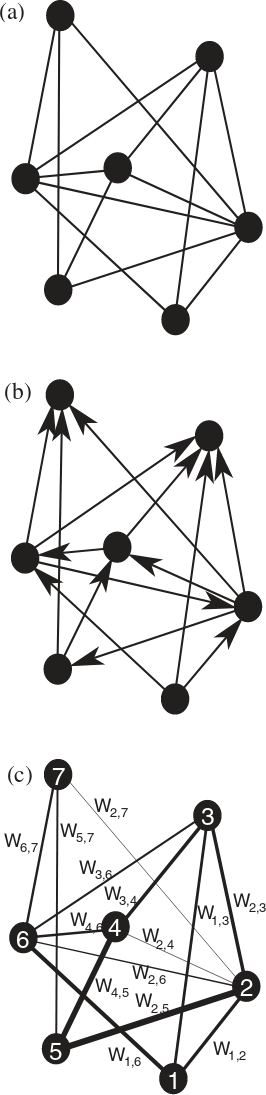
\includegraphics[width=\marginparwidth]{./Figures/intro/network_theory/graph_properties_Boccaletti2006.png}
%\captionof{figure}[Three types of graphs]{An undirected (a), a directed (b), and a weighted undirected (c) graph. From \cite{Boccaletti2006}}
%}
%}
%\end{scriptsize}

Starting with the building blocks of networks, we may define a \textbf{graph} as a pair of sets $G = (V,E)$, where $V = \{v_1,v_2,...,v_n\}$ is the set of \textbf{nodes} of the graph, and $E$ is the set of \textbf{edges}, or links, of the graph connecting pairs of nodes. The set $E$ can be any subset of all ordered pairs of $V$, such that $E \in V \otimes V$. Graphs can be either \textbf{directed} or \textbf{undirected} depeding on whether their constituent links are directional, i.e. whether $[v_i,v_j] \in E$ implies $[v_j,v_i] \in E$ (Fig. 1.1). Further, simple graphs are antirreflexive, meaning that a node cannot be linked to itself, i.e. $[v_i,v_j] \in E$ implies $i \neq j$.

Such a simple configuration can be easily extended by considering weighted or quantitative links. By incorporating weights, a \textbf{weighted graph} is a quadruple $G = (V,E,W,f)$, where $V$ and $E$ are the sets of nodes and edges defined above, $W = \{w_1,w_2,...,w_n\}$ is a set of weights such that $w_i \in \mathbb{R}$, and $f: E \rightarrow W$ is a mapping assigning weights to edges.

Intuitively, we say that two nodes $v_i$ and $v_j$ are \textbf{adjacent} to each other, or connected, if they are joined by an edge $e = \{v_i,v_j\}$. Similarly, two edges are adjacent if they are incident to at least one node.

The most basic structural property of a node is its \textbf{degree}. It is defined simply as the number of links incident to it. In directed graphs, one may distinguish in-degree, the number of links incident to a node, from out-degree, the number of links incident from it.

\begin{figure}[ht]
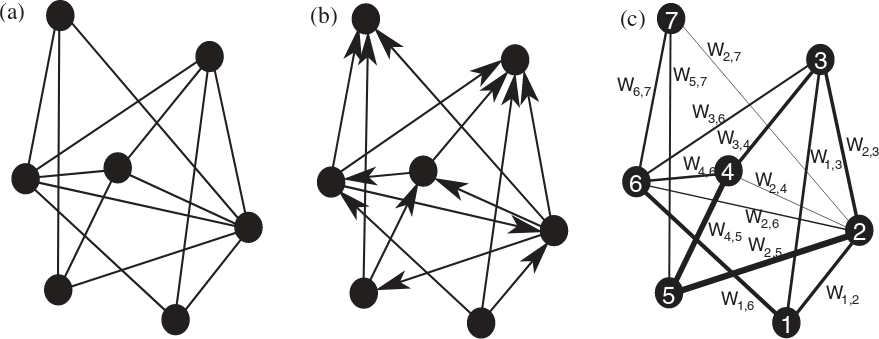
\includegraphics[width=\textwidth]{./Figures/intro/network_theory/graph_properties_Boccaletti2006_horizontal.png}
\caption[Three types of graphs]{An undirected (a), a directed (b), and a weighted undirected (c) graph. From \cite{Boccaletti2006}}
\label{fig:network_types}
\end{figure}

The \textbf{shortest path} connecting two nodes $v_i$ and $v_j$ is defined as the path with the shortest number of edges that connects them. This quantity, $L_{min}$, is also called the \textbf{distance} between two nodes. For weighted graphs, this definition may be refined to consider edge weight, such that the shortest path is the one that minimizes the summed weight of the edges connecting the two nodes.

A graph, in the context of network theory, is termed a \textbf{network}, and we will use this term hereafter. A network is said to be \textbf{complex} when it possesses topological features that are neither random nor completely regular. These features refer to properties of the network as a whole, and three of the most widely studied features of network are their degree distribution, their average path length and their clustering coefficient.

The \textbf{degree distribution} of a network is the probability distribution of the degrees of the network nodes. It is an important property of complex networks, as the degree distributions of random networks differs systematically from that of empirical networks of different types \citep{Barabasi1999}. While randomly assembled networks display Poisson degree distributions, many real networks are best represented as having power-law degree distributions. This means that in real networks, most nodes are typically connected to only a few other nodes (i.e. have a low degree), whereas a small number of nodes are highly connected. Networks with power-law degree distributions are alternatively called \textbf{scale-free networks} (Fig. \ref{fig:scale_free}).

\begin{figure}[ht]
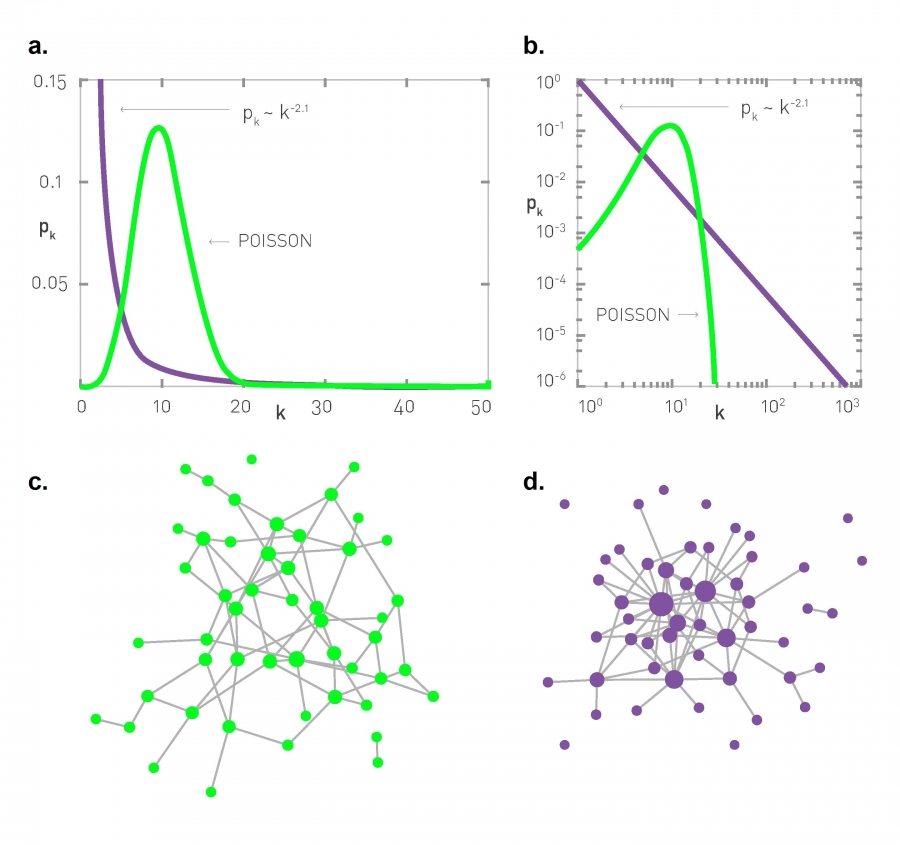
\includegraphics[width=\textwidth]{./Figures/intro/network_theory/degree_distrib_Barabasi2016.jpg}
\caption[Random and scale-free degree distributions]{\color{Gray} Degree distributions from random (green) and scale-free networks (purple) in natural (a) and logarithmic (b) axes. The hubs present in scale-free networks are evident in the network depiction (d). From \cite{Barabasi2016}}
\label{fig:scale_free}
\end{figure}

The \textbf{average path length} of a network is the average of the shortest paths between each pair of network nodes. It is given by

\begin{equation}
L = \frac{1}{S(S-1)} \sum_{i,j=1,S;i \neq j} L_{min}(i,j)
\end{equation}

and gives a measure of connectedness between any pair of nodes. Both random and scale-free networks display characteristically short average path lengths \citep{Montoya2002}.

Another important topological property is the \textbf{clustering coefficient}. It measures the degree to which the neighbours of a given node are linked together. Given a node $i$ with degree $d_i$, its local clustering coefficient is defined as

\begin{equation}
C_v(i) = \frac{2E_i}{k_i(k_i - 1)}
\end{equation}

where $E_i$ is the number of links between the $k_i$ neighbors of node $i$. The clustering coefficient of the network is the average over all $S$ nodes:

\begin{equation}
C_v = \frac{1}{S} \sum_{i=1}^{S} c_v(i)
\end{equation}

When considering network topology, networks without any differentiation between nodes, where each node can in principle interact with any other node, are called \textbf{unipartite}. Another common type of ecological networks is that which represents two disjoint groups that interact with each other but not with members of the same group (for example, a network with a group of plant species and a separate group of pollinators, Fig. \ref{fig:bipartite_nested}). Such networks are called \textbf{bipartite}.

\begin{figure}[ht]
\centering
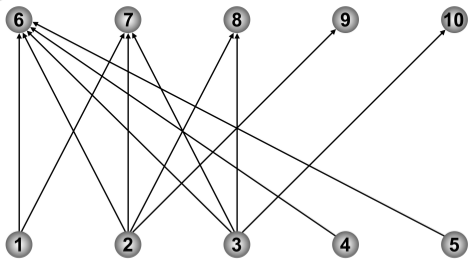
\includegraphics[width=0.5\textwidth]{./Figures/intro/network_theory/bipartite_nested_network_Ings2009.png}
\caption[Nested bipartite network]{\color{Gray} A bipartite network, in which nodes 1-5 and nodes 6-10 form sets that do not have within-group links. The network is also nested: the diet of consumer 8 is a subset of that of consumer 7, which in turn is a subset of that of consumer 6. From \cite{Ings2009}}
\label{fig:bipartite_nested}
\end{figure}

Several other network properties are widely used in the context of ecological networks. Here I will mention three of them. First, the \textbf{connectance} of a network is the proportion of realized links with respect to the potential number of links in the network. It is defined in different ways depending on the assumptions about the feasible links of the network. Four variations are possible regarding the directedness of the network and the feasibility of self-loops. The most general case is a directed network where self-loops are allowed. In that case, the set of potential links is simply $L_p = S^2$ for a network of $S$ nodes. If self-loops are not allowed, the set of potential links is $L_p = S^2 - S$, whereas if the network is undirected, the number of potential links halves, i.e. $L_p = S^2/2$. Therefore, an undirected network with no self-loops has $L_p = (S^2 - S)/2$ potential links. The general definition of connectance is

\begin{equation}
C = \frac{L}{L_p}
\end{equation}

where $L$ is the number of realized links.

The above definitions of the set of potential links imply that, aside from the consideration of self-loops, all links between any pair of species are potentially feasible.

Another topological property widely studied, \textbf{modularity} is the tendency of the network to display modules highly connected within but largely disconnected from each other. The detection of modules, or clusters, in networks is an active area of research, and a closed definition of modularity depends on the expected number of modules and their link distribution. As an example, \cite{Fortuna2010} defined modularity as

\begin{equation}
M = \sum_{s = 1}^{N_M} \left[\frac{l_s}{L} - \left(\frac{d_s}{2L}\right)^2\right]
\end{equation}

Lastly, \textbf{nestedness} is a property of bipartite networks by which nodes with low degree are connected to a subset of the nodes linked by nodes with high degree (Fig. \ref{fig:bipartite_nested}).

Aside from these general definitions, it is important to mention the matrix representation of networks. Intuitively, by defining a matrix $A$ of dimensions $S * S$, its entries $a_{i,j}$ may represent the existence (or weight) of a link between nodes $i$ and $j$. Such matrix is called the \textbf{adjacency matrix}. If the network is undirected, its adjacency matrix is symmetric, i.e. $a_{i,j} = a_{j,i}$

\[
A_{undirected} = \begin{pmatrix}
0& 1& 0 \\
1& 0& 1 \\
0& 1& 0
\end{pmatrix}
\]

where $a_{i,j} = 1$ if a link exists between nodes $i$ and $j$, and $a_{i,j} = 0$ otherwise. If the network is directed, the possibility exists that $a_{i,j} \neq a_{j,i}$, so that an example matrix can be

\[
A_{directed} = \begin{pmatrix}
0& 1& 0 \\
0& 0& 0 \\
1& 1& 0
\end{pmatrix}
\]

The convention for directed networks is that adjacency matrices represent the interaction originating in column $j$ and affecting row $i$, so that in the previous example, there is a link from node 2 to node 1, but not the other way around. %The matrix formulation of networks has particular importance in evaluating the stability properties of the associated system, and thus has been extensively used in studies of ecological dynamics. In the next section, I briefly review early developments on ecological networks and further develop some of the properties defined above.

\subsection{Ecological networks: brief history, recent developments and open questions}

The general definitions outlined above can be applied to ecological systems seamlessly by defining individuals, species or guilds as nodes, and the biotic interactions among them as the edges or links connecting them. Indeed, natural historians and early ecologists had recognized the network nature of ecological communities long before the recent developments on complex networks. The brief historical review that follows draws primarily from the works by \cite{Bersier2007} and \cite{Ings2018}, and the reader is referred to these studies for consulting primary references.

The first documented observations about the interactions of species can be traced back to Ancient Greece, where mutualistic relationships were observed by Herodotus, Theophrastus and Aristotle. In turn, the arab scholar Al-Jahiz is believed to have introduced the concept of food chain in his \textit{Book of the Animals}, in the 9th-century. In the early Enlightenment the documented study of the natural world began to gain back attention, although admittedly on a secondary position with respect to mathematics, physics, chemistry or astronomy, disciplines that constituted the main focus of the Scientific Revolution. Observations about empirical food chains are documented by van Leeuwenhoek and Linnaeus, but it would be Alexander von Humboldt in the 19th-century, throughout all his works, the first and most influential proponent of a view of nature that emphasized the complex web of relationships between species, looking at nature as a ``living whole''. The first representation of a full network of trophic interactions dates from 1880, and was made by the italian scientist Lorenzo Camerano.

After these and other seminal contributions, the 20th-century saw the confirmation of network-oriented approaches to ecological issues. The ecologist Charles Elton developed many important concepts, such as the ``pyramid of numbers'' by which abundances decreased along the food chain, and established the terms \textit{food chain} and \textit{food cycle}. After his seminal works, the network representation of trophic relationships became a common framework for studying ecological communities. By this point, trophic relationships were already the most studied interactions in ecological communities. Trophic interactions are ubiquitous in nature, they are usually the easiest to document and, unlike other interactions, can be used to outline the fluxes of biomass and energy in a given community. It is, therefore, not surprising that they took, and still maintain, such a predominant role in studies of ecological networks. The figure of Raymond Lindeman also stands out in the first half of the 20th century, with his work ``The trophic dynamic aspect of ecology'', in which he studied for the first time the quantitative fluxes and feedbacks between the biotic and abiotic components of an entire ecosystem, the Cedar Bog Lake in Minnesota \citep{Lindeman1942}. As \cite{Ings2018} note, limnology had a prominent position on these early developments, and many temperate lakes were the first ecosystems to be thoroughly sampled and studied.

In parallel to these insights from natural systems, the mathematical foundations for studying the dynamics of ecological interactions were being developed. The mathematician Alfred J. Lotka proposed in 1920 a set of equations for the population dynamics of a pair of predator and prey species, that explained the apparent oscillations observed in plant-herbivore systems \citep{Lotka1920}. In an independent contribution another mathematician, Vito Volterra, derived similar equations following observations of fish catches in the Adriatic Sea \citep{Volterra1928}. The general form of these equations is

\begin{equation}
\begin{array}{c}
\frac{dx}{dt} = \alpha x - \beta xy \\
\frac{dy}{dt} = \delta xy - \gamma y
\end{array}\label{eq:LV}
\end{equation}

where $x$ is the number of prey, $y$ is the number of predators, $\alpha$ is the growth rate of the prey, $\beta$ the predation rate coefficient, $\delta$ the predator's growth rate, and $\gamma$ its mortality rate. In this model, both species modulate their abundances in response to the other (Fig. \ref{fig:LV_example}), and the non-trivial solution to the system, formulated as with eq. \ref{eq:LV} is stable and periodic. The Lotka-Volterra set of equations implies a series of assumptions about the underlying biological system. First, they are an example of a mean-field system, thus assuming an homogeneous habitat in which individuals are interacting without constraints or variations. Prey populations in the absence of the predator display exponential growth (i.e., if $ y = 0$, the variation in prey density is given by $\alpha x$), and the predator depends entirely on the prey population. Furthermore, predators do not satiate, in that they respond instantaneously to increases in prey population. Importantly, all $\alpha , \beta , \delta , \gamma$ coefficients are constant, thus assuming no other sources of variation.

\begin{figure}[ht]
\centering
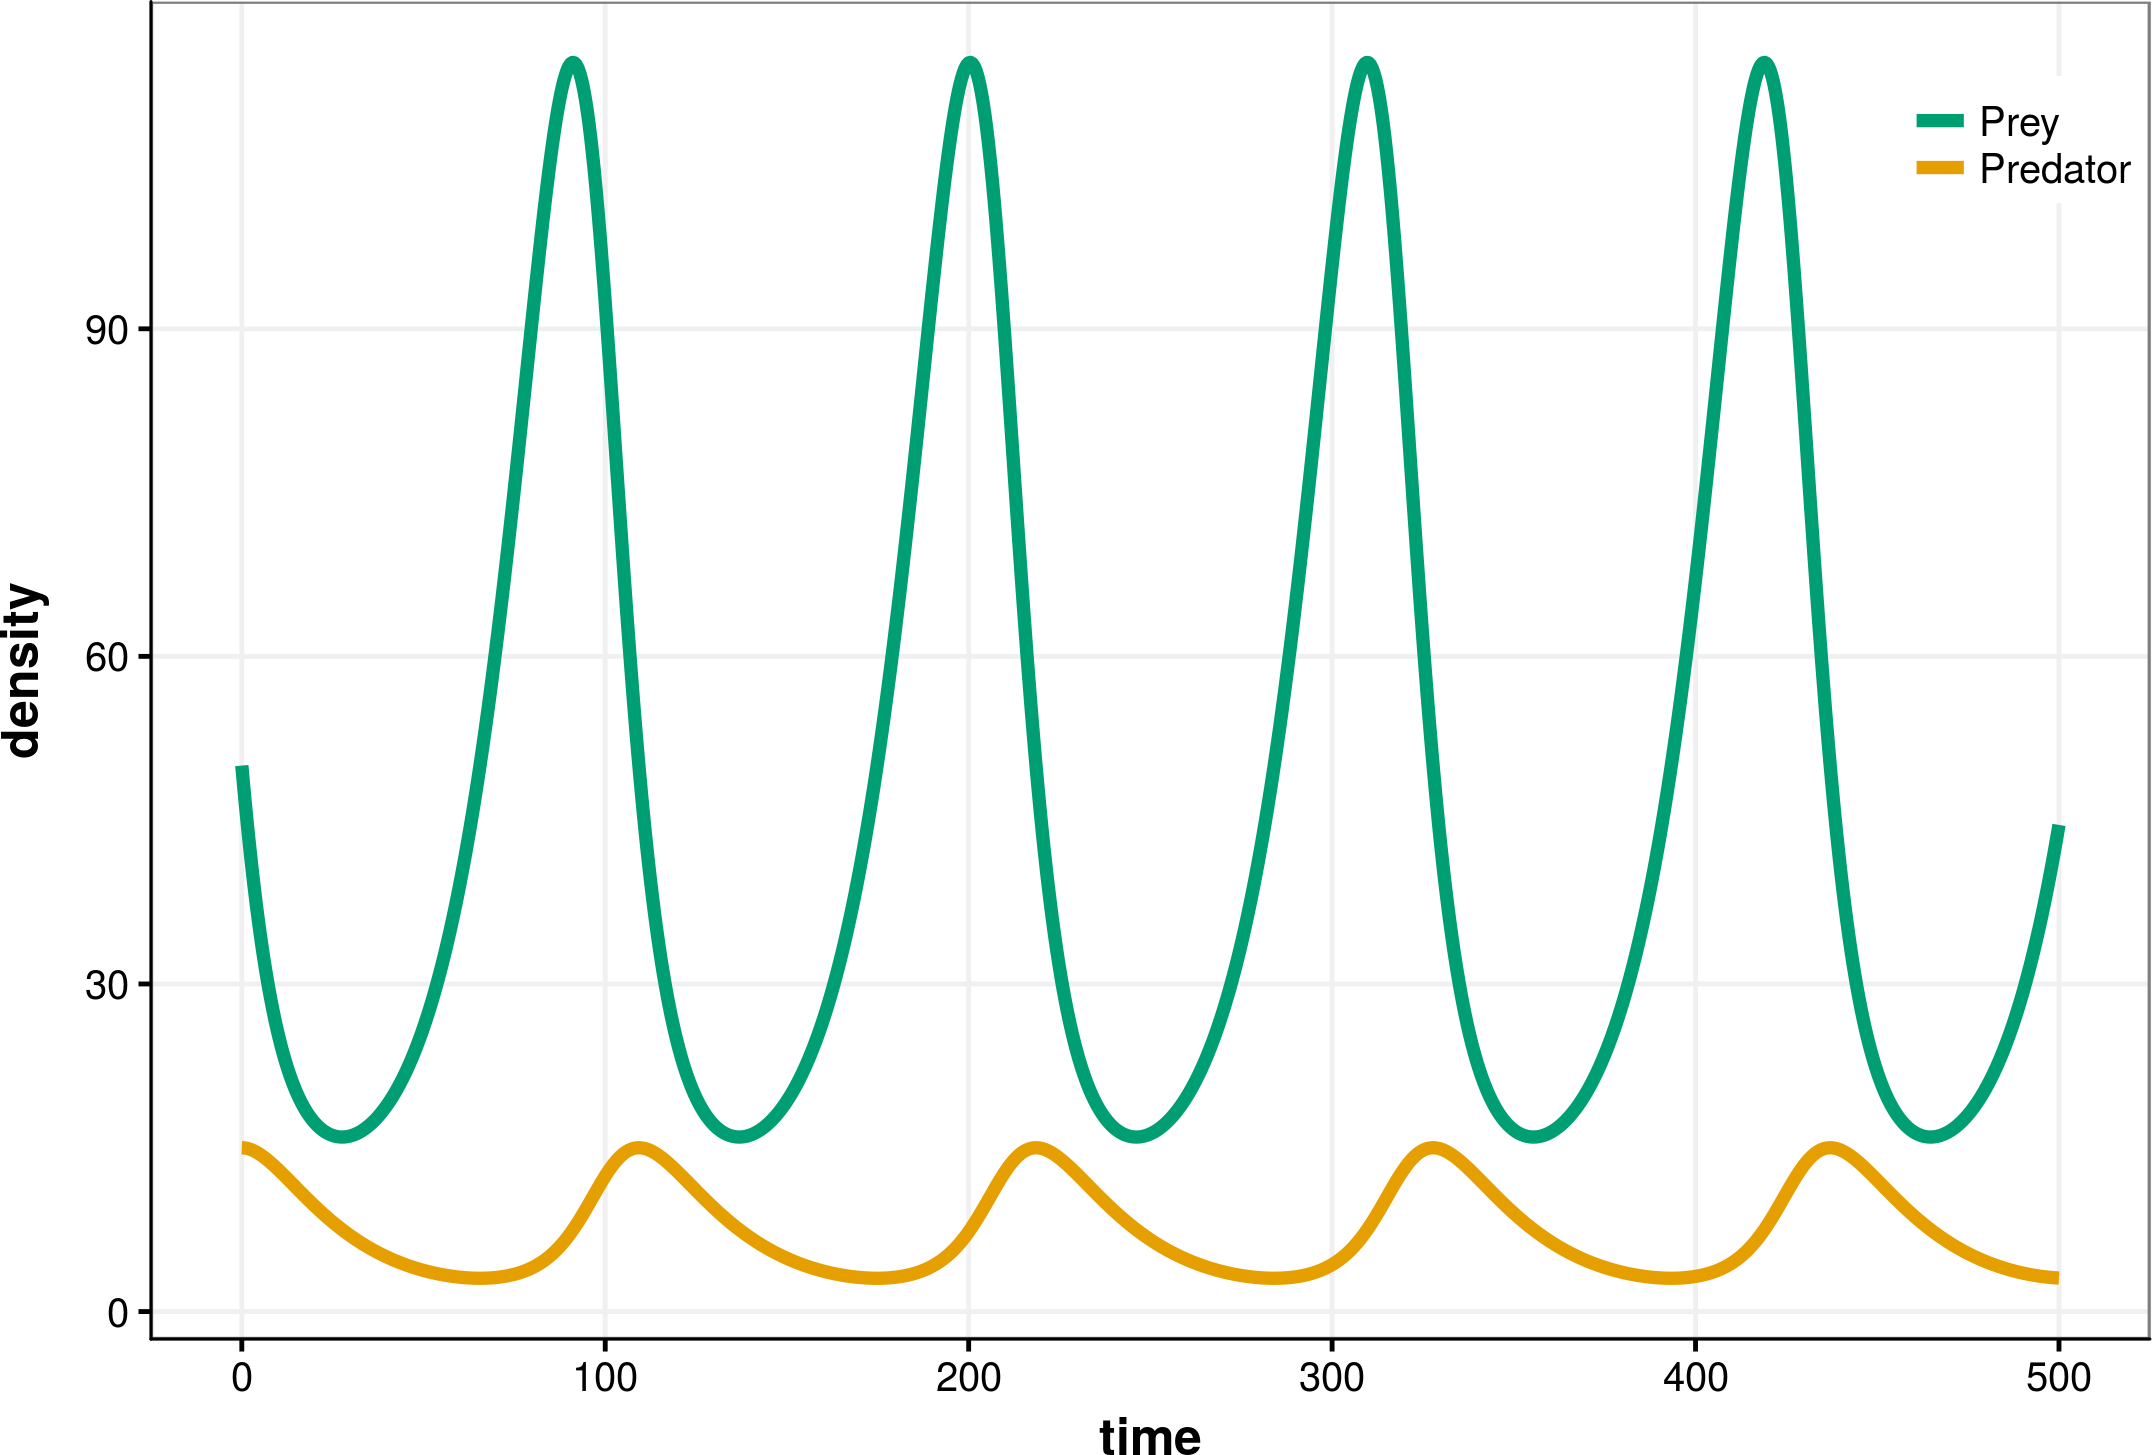
\includegraphics[width=.75\textwidth]{./Figures/intro/ecological_networks/LV_example.png}
\caption[2-species Lotka-Volterra system]{\color{Gray} Lotka-Volterra equations generate stable population dynamics in which densities of the prey and the predator species are both dependent on each other.}
\label{fig:LV_example}
\end{figure}

In the context of dynamical systems, the stability of the system can be approached by analysing how the system responds to very small perturbations off a steady state. This is done by calculating the \textit{eigenvalues} of the system, values that encapsulate the response of the system to such a small perturbation around the equilibrium. The mathematics behind the calculation and interpretation of eigenvalues have been thoroughly developed, and the interested reader may find innumerable derivations of it. In the context of ecological networks, the book \textit{Food Webs} by Kevin \cite{McCann2011} gives a well-balanced introduction to the study of dynamical systems. The important message is that the eigenvalues of a dynamical system (in particular, the maximum eigenvalue) are informative about the stability of the system. Positive eigenvalues will imply that the system is locally unstable, whereas negative eigenvalues mean that the system is locally stable around that particular equilibrium.

Despite the initial insights from 2-species model systems, many ecologists were, as we have seen, much more interested on the notion of stability of whole communities or ecosystems. The first conceptual treatments of community stability can be traced back to Eugene Odum, who suggested that in a community, the number of alternative paths a quantum of energy has for going from primary producers to top predators is a measure of the stability of the community. This notion that the more links an ecological network had, the more stable it was (or, in other words, that ``complexity begets stability''), was the prevalent opinion up until the early 70s. Robert MacArthur, in another highly influential study, analyzed the stability of complete food webs in a semi-quantitative way. He arrived to the hypothesis that community stability increases by either increasing the number of species in a community, or the connectance of the associated food web \citep{MacArthur1955}.

The complexity-stability dichotomy of ecological communities entered a new dimension after the seminal work of Robert May \citep{May1972}, who used for the first time mathematical models of idealized communities to assess the local stability of systems with an indeterminate number of species modelled with Lotka-Volterra dynamics. He found that, in randomly assembled networks with normally distributed interaction strengths, the dynamical systems remain locally stable if

\begin{equation}
\alpha \sqrt{SC} < 1\label{eq:May}
\end{equation}

where $\alpha$ is the average interaction strength, $S$ is the number of species, and $C$ is the connectance of the network in the form $L/S^2$. The interpretation is that an increase in either mean interaction strength of the system, species richness, or number of links, would rapidly tend to destabilize the system. Crucially, May was of course aware of the limitations of his approach: the assembled networks possessed no structure whatsoever, pairwise interaction strength was assumed to be a constant, stochastic parameter, and the definition of stability involved infinitesimally small perturbations from an equilibrium state, as given by the eigenvalues of the system. Nevertheless, regardless such obvious limitations, May's work was the first quantitative derivation about the expected stability of arbitrarily large ecological communities, and not only so, but it also was a frontal attack on the common wisdom championed by MacArthur (who passed away way too early, in 1972) and many others by that time. The debates and number of studies triggered by May's results are countless, both in the camps of the theoreticians and the empiricists. From that moment onwards, the study of ecological networks started to gain even more attention and took many different parallel paths. An important line of research, that did not start with May's results but definitely gained attention after them, follows the estimation of interaction strengths both in theoretical studies of functional responses \citep{Holling1965} and empirical estimations \citep{Bender1984}.

Robert Paine showed in 1966 that the effects of removing a top predator could propagate throughout the whole ecological network, eventually altering the richness of the community \citep{Paine1966}. This striking result led to the denomination of \textit{keystone species} to those species with a disproportionate influence in the overall structure and dynamics of the community. He continued to be interested in measuring the impacts of one species over another and on the overall community, a theme that came together with the theoretical importance of interaction strength proposed by May. Theoretical metrics of interaction strength represent changes in different per capita or population-level parameters \citep{Laska1998} but such metrics are, importantly, not generally equivalent to what is measured in experimental studies (e.g. \citealt{Bender1984}). Paine observed that descriptions of food webs that failed to account for estimates of interaction strengths were not enough in order to link the structure of food webs with their dynamical behaviour \citep{Paine1992}.

However, obtaining empirical estimates of all interaction strengths in a given network is so far unfeasible even for moderately rich communities, given the complexity of the combinations and feedbacks of effects between the different species involved. This divide between theoretical models and empirical estimates of interaction strengths is still one of the main unresolved problems in network ecology. Theoretically, it has been shown that, within the framework of local stability analyses and for networks considering only trophic interactions, stability is enhanced when a majority of interactions are comparatively weak and only a few are comparatively strong \citep{McCann1998,Berlow1999}. Incidentally, a recent article showed this pattern to hold in a set of empirical food webs \citep{Jacquet2016}.

Aside from the studies on theoretical and empirical interaction strength, and its importance on community stability, another strong source of discussion arising from May's results is the role that non-random structural patterns played in conferring stability to empirical networks. The first empirical food webs to be collected and analysed for structural regularities approach in the late 70s, in particular in a seminal book by Joel \cite{Cohen1978}. An early focus of studies on food web structure was the role of \textit{connectance}, given its relationship to theoretical stability (eqn. \ref{eq:May}). Early efforts tested, for example, the potential invariance of the relationship between number of links and number of species $L/S$, as a means of corroborating May's criterion (see \citealt{Pascual2006} for details).

The early compilations of empirical food webs, however, were not even close to be complete descriptions of their systems, and had important flaws such as differential level of node taxonomic aggregation. Newly collected data in the early 1990s \citep{Polis1991, Martinez1991} showed that network metrics and relationships outlined with earlier food webs were in many cases artifacts of the poorly collected data \citep{Pascual2006}, and this realisation triggered a reorientation of efforts and development of new hypotheses and ideas concerning food web structure. Among them, an important theoretical model of food web structure, the niche model \citep{Williams2000}, proved able to generate food webs with realistic structural patterns out of a single niche axis in which all consumer species are sorted. More recently, species-level traits and their distribution have proven to be important in characterizing food web structure, as shown for example by \cite{Laigle2018}.

In parallel to these more recent developments on food webs, studies on other types of interactions started to emerge in the late 20th century. The first attempt at characterizing a network of positive interactions was made by Pedro \citet{Jordano1987}, who studied patterns of connectance and interaction strength in plant-pollinator and plant-seed disperser networks. From his seminal study, a whole field of research opened up, and the study of bipartite mutualistic networks has produced many insights regarding the structure and dynamics of these communities \citep{Vazquez2009a, Bascompte2013}. In particular, bipartite mutualistic networks have been shown to be generally nested, and this nestedness is an important feature for their stability, as opposed to food webs, which are thought to be comparatively less nested and more modular \citep{Thebault2010}.

It is now sufficiently clear that, in any case, mutualistic interactions are structured in a non-random fashion in empirical bipartite networks, and this structure has important consequences for their dynamics. Regarding the study of interaction strengths in mutualistic networks, the functional responses of mutualism are much less studied than those of predator-prey interactions \citep{Holland2002}, and a novel line of research focused on estimating the net impact of a species over another by using as a surrogate their interaction frequency \citep{Vazquez2005}. This approximation is likely dependent on the specific type of mutualism considered. For example, in a study analysing plant-hummingbird networks, \cite{Vizentin-Bugoni2014} showed that trait-matching was more important for structuring these ecological networks than abundances alone. In further studies, interaction frequency itself has been found to be well approximated by the abundances of the interacting species \citep{Vazquez2007}. This methodology for estimating population-level short-term impacts is thus promising for mutualistic networks in which no other quantitative effects are available. Importantly, the approximation hinges on interactions being stochastic, with no trait-mediated selection of interaction partner or frequency. In that sense, it may also serve as a baseline against which to compare the effect of traits in specifying interactions \citep{Poisot2015}.

All in all, the knowledge about the structure and dynamics of single-interaction ecological networks has increased enormously in the last few decades. A fundamental question that we may ask is the extent to which these varied insights are applicable to empirical, complex communities. Despite the convenient distinction between interaction types commonly made for studying ecological networks, communities are composed of individuals interacting in many different ways, with varying intensities and at different spatial and temporal scales.

We know now that, at the very least, both predator-prey and mutualistic interactions are highly structured in empirical communities. We lack, however, a general framework for ecological networks in which different interaction types are integrated, and where the combined structure of the network can be analysed. This integration, of course, will have important implications for community dynamics: for example, including non-trophic interactions onto food webs has already been shown to importantly alter their stability patterns \citep{Kefi2012, Kefi2016a}, or their robustness to secondary extinctions \citep{Pocock2012}. This change of scope about ecological communities may also trigger novel questions about their structure and dynamics. It may seem surprising on a first look, but we currently do not know how the different interaction types are distributed in empirical communities generally. Actually, given the difficulty of compiling different interaction types in a systematic way for any relatively rich community, it becomes clear that approaching such a fundamental question requires important observational and experimental efforts. In that sense, a general theoretical framework for multiple interactions networks may help develop targeted hypothesis about empirical communities, from which to build observational or experimental studies. Related important questions concern the role of spatial patterns or environmental gradients in shaping the combined structure of ecological networks. For example, does the spatial structure of the different interaction types vary? How does this influence the spatial propagation of effects? Does the relative importance of the different interaction types vary across environmental gradients?

In single-interaction networks, the role of space in shaping their structure and stability has been recognised as a key factor, e.g. by analysing how different communities are connected by dispersal and the implications for the overall metacommunity \citep{Leibold2004}, or how network structure varies with spatial scale \citep{Galiana2018}.

In order to integrate recent advances on multiple interactions networks with the spatially explicit framework of metacommunity ecology, some issues need to be resolved before a proper multiple interaction metacommunity framework is developed. For example, what is the nature of the connections between spatially separated communities? Mobile species are capable of displacements in order to look for food sources (antagonism, mutualism), or in order to establish themselves in another territory (dispersal). It is important to know if there is a relationship between the movement capacity of a given species and its tendency to engage in different interaction types. It is also important to develop theory on the spatial propagation of interaction effects: how do the different types of interaction propagate in space? Are some interaction types more likely to have a greater impact on the overall community than others? Or is the effect only related to the relative magnitude of the interaction, and the centrality of the species involved?

Some of these questions have been barely explored even in metacommunities of single interaction types. Most metacommunity studies follow the long-standing history of horizontal communities and consider how competitive guilds are connected in space, and only recently is metacommunity theory being expanded to account for mulitrophic networks \citep{McCann2005, Fahimipour2014, Gravel2016a}. It is therefore necessary to strenghten the foundations of metacommunity theory before integrating it with the paradigm of multiple interactions networks.

From a more general point of view, one can also ask whether the structure and dynamics of ecological networks vary across different types of gradients, and if so, what are the factors and processes driving this variability. The variability of ecological interactions across environmental gradients has been studied under different subfields of community ecology, from the point of view of horizontal communities (mainly plants: the Stress Gradient Theory, see e.g. \citealt{Maestre2009}) and theoretical food webs with competitive interactions (Environmental Stress Models, see \citealt{Menge1987}). Stress Gradient Theory focuses on evaluating the response of communities to variations in environmental stress, and does so by studying plant communities which, as stated by theory and empirical observations, may exhibit variations in the relative importance of competitive versus facilitative interactions as stress increases \citep{Callaway1997}. This theory, however, is currently not applicable to multitrophic communities, despite recent attempts to test its validity for higher trophic levels \citep{Barrio2013}. Environmental Stress Models, in turn, were developed to predict the differential role of top-down and bottom-up processes in food webs across gradients of environmental stress. While theoretically comprehensive, their difficulty of testing has prevented further developments except for localised, targeted systems (e.g. \citealt{Cheng2016a, Daleo2015}). In any case, none of these theories incorporates the whole array of interactions potentially occurring in nature, and a further issue is that the different types of environmental gradient that mediate ecological processes are usually taken together, without differentiating the different environmental components that may affect interactions and demographic processes. Therefore, we are still far from a general theory on ecological networks and their variability across environmental gradients.

\section{Objectives}

In my thesis I addressed fundamental unresolved questions about ecological networks in general. Chapters 2 and 3 deal explicitly with networks of multiple interaction types, and the rest of the thesis explores fundamental questions for which more simple model systems are used, in order to focus on the specific questions at hand before adding the complexity of multiple interactions. The following general objectives constitute the main chapters of the thesis:

\begin{itemize}
\item \textbf{To review and synthethise current methodologies for modelling multiple interactions in ecology}\\ \\
First, I aimed to synthesize and organize the growing literature on this type of networks, while at the same time laying down some methodological foundations for future theoretical studies on the subject.

\item \textbf{To understand how the frequency and distribution of the different interactions drive species persistence}\\ \\
Second, I developed a general theoretical model in which I tackle several key issues about network structure and dynamics. I aimed at deriving general hypotheses about the persistence of species in complex networks with realistic structural patterns.

\item \textbf{To know how Species Abundance Distributions are influenced by the structure of multitrophic communities}\\ \\
Third, I looked at a classic pattern from horizontal community ecology, the Species Abundance Distribution, from a network perspective. In order to understand how the frequency and/or distribution of interaction types influences the distribution of abundances in a given community, first it is necessary to develop theoretical expectations about its distribution on more simple networks, for example food webs. I drew from the extensive literature on food webs and trophic relationships in general to derive basic hypothesis about the variation of Species Abundance Distributions across trophic guilds.

\item \textbf{To advance in the understanding of interaction effects in space}\\ \\
Fourth, I studied the role of space in propagating interaction effects. As with the previous chapters, no general hypotheses exist about the spatial propagation of interaction impacts, so in order to provide baseline expectations and for our study to be comparable to previous efforts, I focused on the effect of trophic interactions and how they propagate when species disperse or forage in a set of spatially connected communities.

\item \textbf{To explore whether environmental factors drive the frequency of different types of interactions}\\ \\
Fifth, I studied how interactions are likely to vary across environmental gradients. This issue has been explored independently in different subfields of community ecology, but the conclusions obtained have been largely overlooked in other fields. I recovered the classic differentiation in environmental factors first proposed by Hutchinson and delve in how gradients in different types of environmental factors may drive variations in the prevalence of different interaction types and other community properties. Given the paucity of studies and theory in this question, I took the same approximation as in chapters four and five, and resorted to basic horizontal communities, in order to provide general foundations from which ideas about more complex communities can be developed.

\end{itemize}

%%************************************************
\chapter[Multiple Interactions Networks]{Multiple interactions networks: towards more realistic
descriptions of the web of life}\label{ch:review}
%************************************************

\tikz[remember picture,overlay] \node[opacity=0.3,inner sep=0pt] at (current page.center){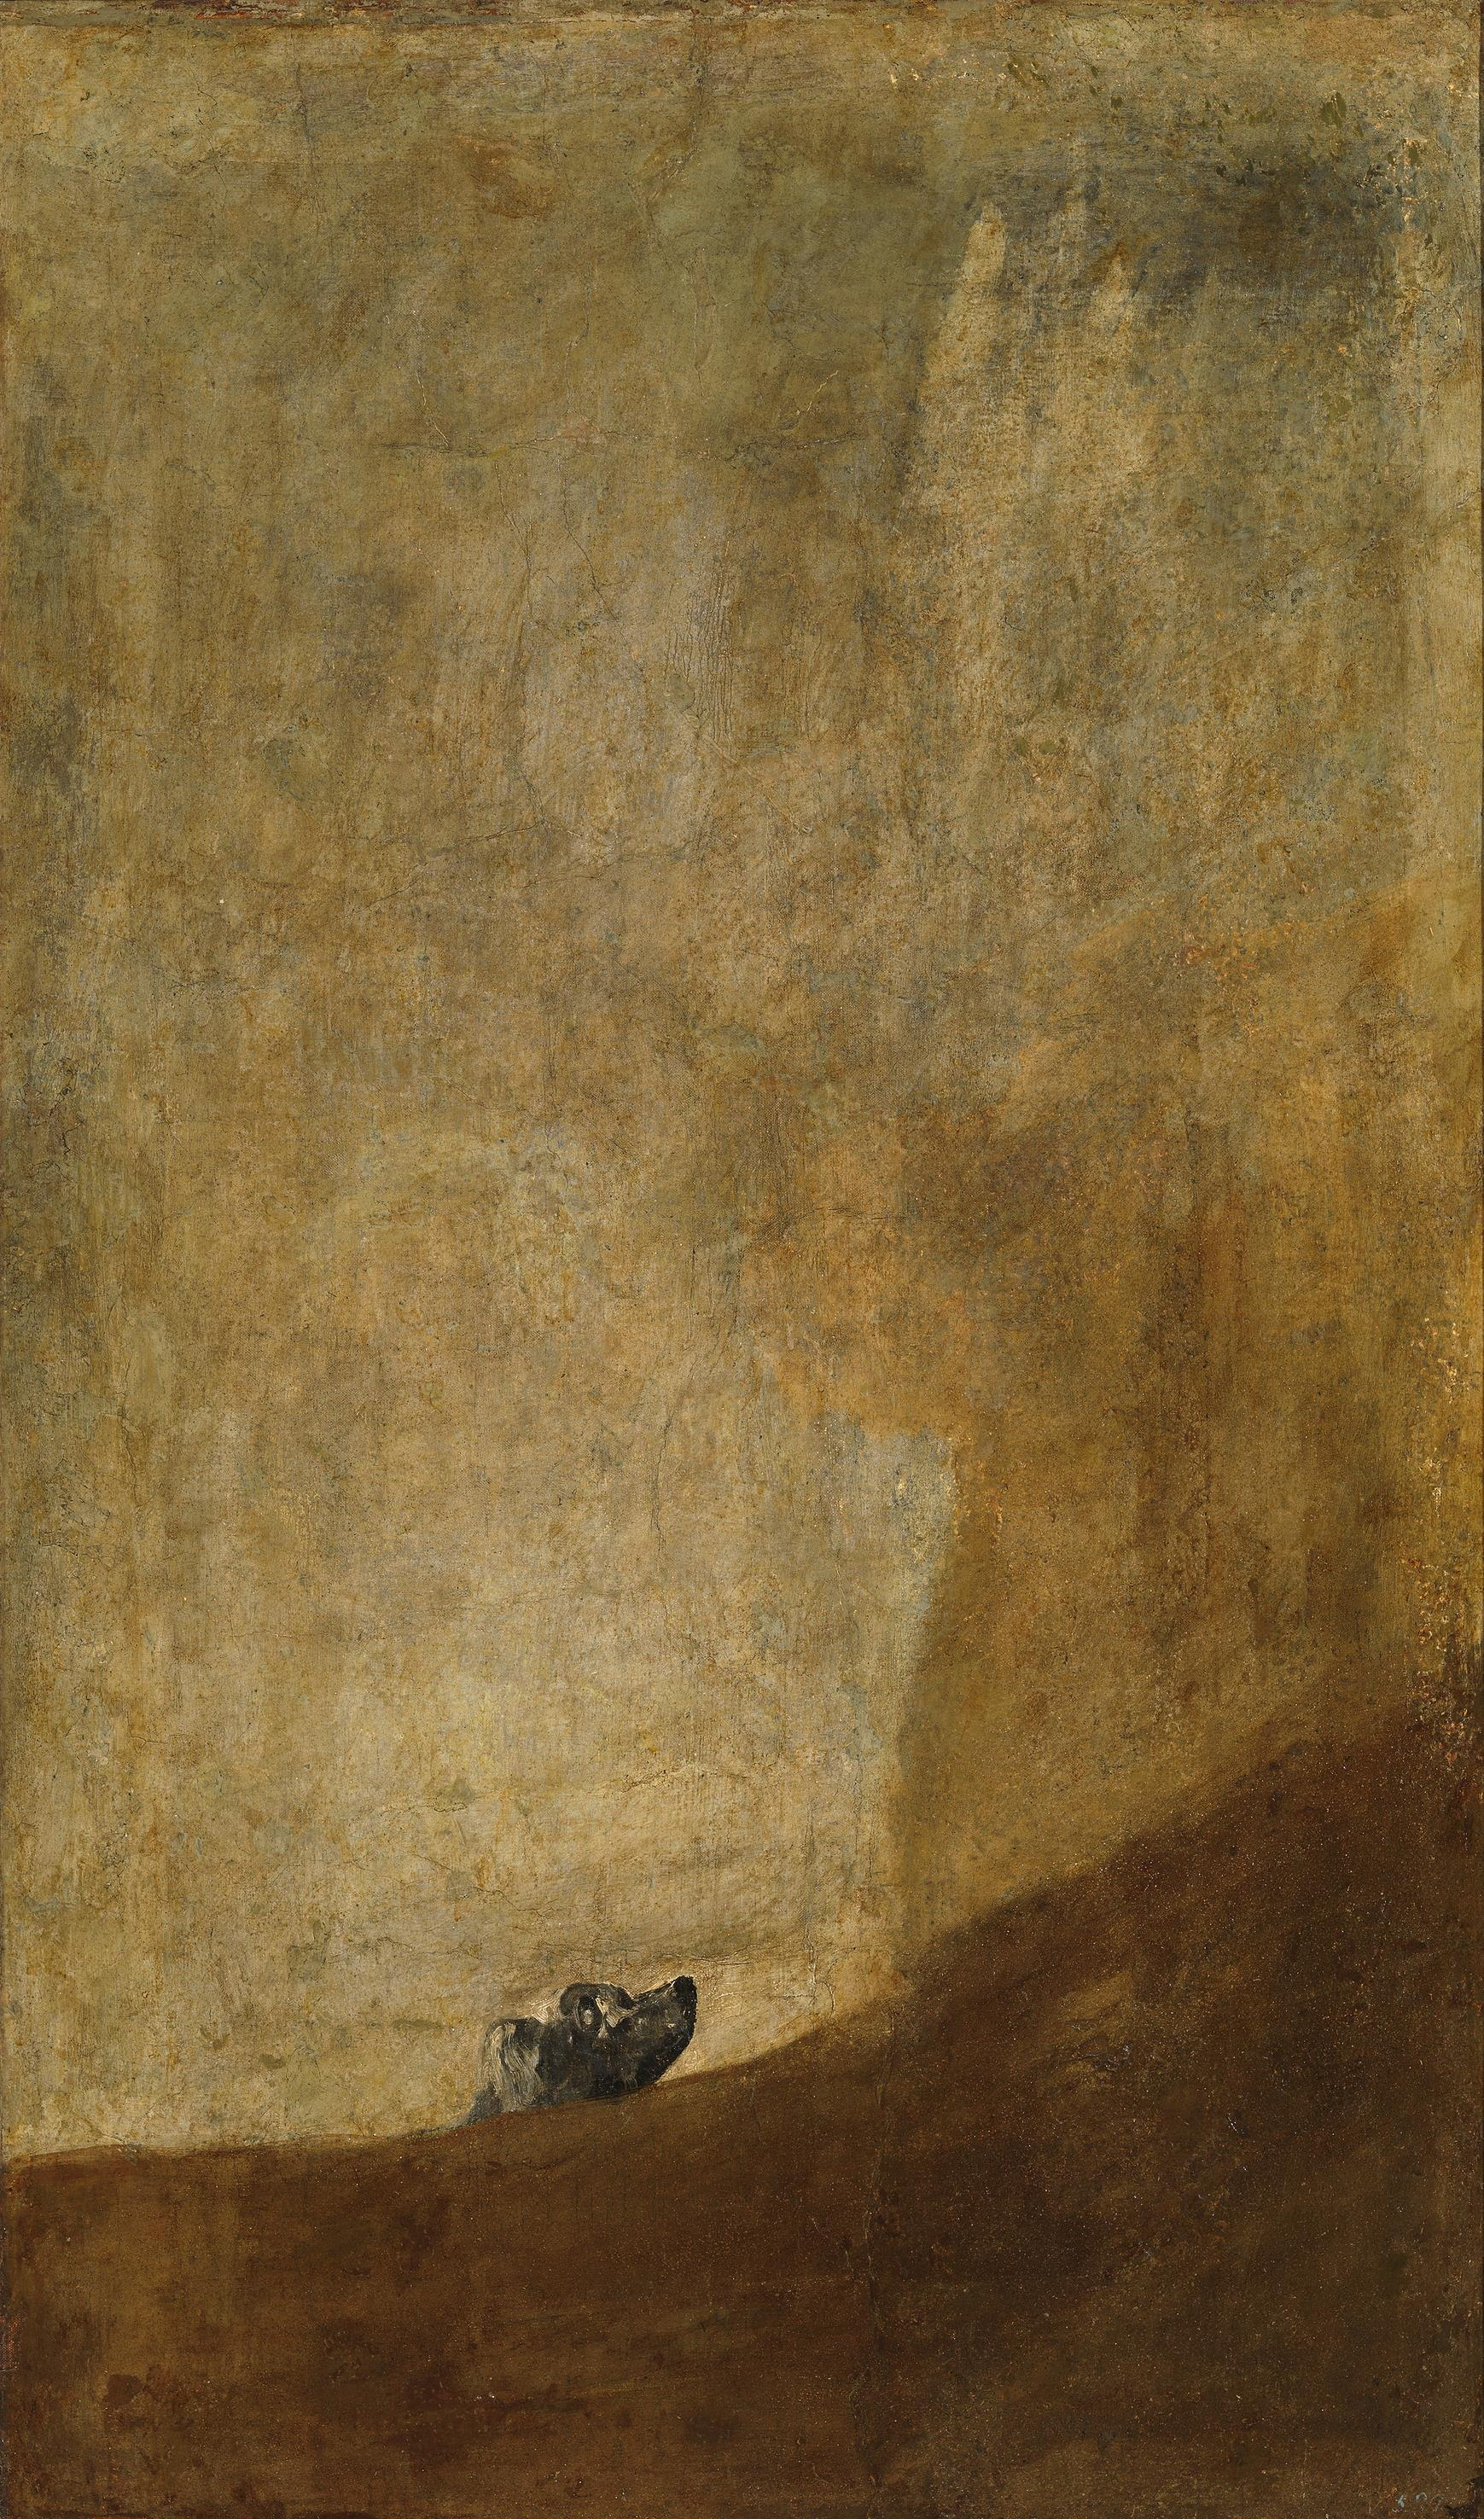
\includegraphics[width=\paperwidth,height=\paperheight]{./Figures/cover/Goya_Dog.jpg}};
\clearpage

\section*{Abstract}
Ecological communities are defined by species interacting dynamically in a given location at a given time, and can be conveniently represented as networks of interactions. Pairwise interactions can be ascribed to one of five main types, depending on their outcome for the species involved: amensalism, antagonism (including predation, parasitism and
disease), commensalism, competition or mutualism. While most studies have dealt so far with networks involving one single type of interaction at a time, often focusing on a specific clade and/or guild, recent studies are being developed that consider networks with more than one interaction type and across several levels of biological organisation. We review these developments and suggest that three main frameworks are in use to investigate the properties of multiple interactions networks: ‘expanded food-webs’, ‘multilayer networks’ and ‘equal footing networks’. They differ on how interactions are classified and implemented in mathematical models, and on whether the effect of different interaction types is expressed in the same units. We analyse the mathematical and ecological assumptions of these three approaches, and identify some of the questions that can be addressed with each one of them. Since the overwhelming majority of studies on multiple interactions are theoretical and use artificially generated data, we also provide recommendations for the incorporation of field data in such studies.

\section{Community ecology and network theory}
Ecological communities should be defined not only by lists of co-occurring species, but also by the myriad of interactions taking place among them. A convenient way to include information about both species composition and their interactions is to represent communities as networks in which species are nodes connected by links representing biotic interactions. Network analyses can provide insights into community local stability \citep{Allesina2012} and robustness to extinctions \citep{Riede2011a}, the degree of specialization of individual species or guilds \citep{Dorado2011}, the impact of invasive species or climate change on established communities \citep{Lopezaraiza-Mikel2007} and, more generally, on any question in which pairwise interactions relate to community patterns and processes.

Networks can accommodate different types of data, depending on the nature of the links between species (e.g., qualitative, quantitative, static, dynamic), the temporal and spatial resolution of the community, the level of aggregation of the nodes (e.g., individuals, species, trophic guilds), or the specific objectives of the study. A common simplification is to study networks of a single interaction type, e.g., trophic \citep{McCann2011} or mutualistic \citep{Bascompte2013}, assuming (often implicitly) that the effect of other interactions on community dynamics is negligible compared to the ones analysed. Such an assumption is usually unavoidable given the lack of comparable data on different interaction types, but it is becoming increasingly clear that the effects of interactions not accounted for in analyses of single-interaction networks (including indirect ones; but see \citealt{Cazelles2016}) might be significant for species persistence \citep{Soliveres2015a, Kefi2016a} and community structure \citep{Sander2015, Golubski2016}. Furthermore, analyses of interaction networks of a single type often yield differential results regarding the factors that drive their stability. For example, among the factors reported to stabilize food webs are high modularity and low connectance \citep{Thebault2010}, correlation in pairwise interaction strengths \citep{Tang2014}, trophic coherence \citep{Johnson2014}, a preponderance of weak \citep{McCann1998} and asymmetrical interactions \citep{Bascompte2006}, degree distributions broader than those of random graphs \citep{Allesina2015}, or the appearance of generalist consumers coupling resources with different interaction strengths \citep{Rip2010}. On the other hand, mutualistic networks are thought to be more stable when highly nested and connected \citep{Thebault2010, Lever2014}, when there are demographic responses to interactions \citep{Lee2015}, or when mutualistic interactions are relatively strong \citep{Rohr2014}. The persistence and resilience of communities defined with multiple interaction types, however, will additionally likely be influenced at least by (1) the proportion of the different interaction types, (2) the relative strength of pairwise interactions both within and among interaction types, and (3) the structural properties of each sub-network and the overall aggregated network.

The study of single-interaction networks in ecology has progressed enormously in the last decades, both theoretically and empirically. In parallel, the analysis of multiple interactions networks has also advanced in other fields of study \citep{Boccaletti2014}. This novel paradigm has only recently started to be applied to ecological studies, with several examples of new conceptual developments being forged together with applications of old concepts to new problems (Table \ref{tab:table1.1}). Despite the relatively small number of studies using multiple interactions networks in ecology, the research objectives and methodologies that have been addressed are extremely diverse, and a synthesis of recent developments is timely. Here, we identify three main approaches for the design and analysis of ecological multiple interactions networks. These approaches have been used in theoretical and empirical studies without an explicit recognition of their conceptual underpinnings. We define them explicitly, examine their underlying ecological assumptions, the type of questions best addressed with each approach, and provide recommendations for the integration of empirical data.

\section{Multiple interactions networks in ecology}
Probably, the first study of ecological networks explicitly considering different interaction types was the classic study by \cite{May1972}, in which he assembled interaction matrices with random coefficients from a Gaussian distribution  $N{\sim}\left(0,\sigma \right)$  , thereby allowing for negative and positive pairwise interactions to be considered. May's results showed that in theoretical communities assembled randomly, complexity (measured as connectance and species richness) was inversely related to the local stability of the system. But natural communities are highly complex, diverse and, nonetheless, seem to persist. After that seminal study, there has been a flurry of studies trying to uncover the processes and structural patterns that confer stability to empirical communities (e.g. \citealt{Saint-Beat2015}). However, comparable data on different interaction types is extremely difficult to acquire, and the focus for most of the second half of the 20th century has been on how competitive and antagonistic interactions drive population and community patterns (e.g. \citealt{Connell1961, Paine1966}). As predator-prey interactions are easiest to observe and document in the field, the analysis of empirical networks relied almost entirely on food webs for a few decades. Pioneering works by \cite{Jordano1987}, or \cite{Fonseca1996}, amongst others, paved the way for the study of mutualistic networks, but the first studies considering more than one interaction type in the same network only appeared in the last decade (Table \ref{tab:table1.1}).

Developing a theoretical framework for multiple interactions networks involves the integration of a variety of interaction types and effects, direct and indirect, taking place at different temporal and spatial scales. In this review, we propose two main criteria for classifying such frameworks. The first is the classification system applied to interactions \citep{Abrams1987}. Interactions can be defined based on the effect they produce on each member or, alternatively, on the mechanism by which the interaction is produced. Regarding effects, each interactor can be affected positively, negatively, or not affected at all by a pairwise interaction, regardless of the actual mechanisms by which the effect occurs. For example, a (-,-) interaction, defined as competition, could actually be realized through mechanisms as different as territorial, chemical or consumptive competition \citep{Schoener1983}. By defining all interactions with respect to the effect on each member (0,-,+), every effect-based classification is complete, in the sense that no interaction, however idiosyncratic, is left unclassified. Regarding mechanisms, interactions are defined according to the mechanism by which they take place, regardless of the effect on the interacting species. Thus, consumptive competition would be defined as an interaction in which each member is affected by consumption of a common limited set of resources, territorial competition would represent limitations on the available space for each interactor, and so on. A virtually unlimited number of interaction categories can be theoretically defined under this scheme, depending on the questions addressed.

The second criterion distinguishes network analyses based on whether the strengths of different interaction types have common units (i.e., their effects are comparable, acting upon the same population property) or not. This criterion only applies to classification schemes based on effects as, by definition, strengths of interactions acting explicitly through different mechanisms have different units, and are thus not amenable to being homogenized. For example, chemical competition between two plant species may be reflected on the mortality rates of the interacting populations, while a mutualistic interaction between a plant species and a seed disperser bird may affect the dispersal rate of the plant and the population growth rate of the bird. In an effect-based classification with the same units for every interaction, on the contrary, these and every other interaction could be taken to affect a single property (e.g. long-term population size), and hence would be comparable. Based on the two criteria proposed here, we distinguish three conceptual frameworks, already found in the literature, to construct and analyse multiple interactions networks: expanded food webs, multilayer networks, and equal footing networks (Fig. \ref{fig:fig2.1}).

\afterpage{
\clearpage% Flush earlier floats (otherwise order might not be correct)
%\thispagestyle{empty}% empty page style (?)
\begin{landscape}% Landscape page
\begin{footnotesize}
%\begin{longtable}{p{1.5cm}p{1.5cm}p{2cm}p{2cm}p{1.5cm}p{2cm}p{4cm}}
\begin{longtable}{p{1.5cm}p{1.5cm}p{2cm}p{2cm}p{2cm}p{2cm}p{4cm}}
\caption[Studies of multiple interactions networks]{\color{Gray}Studies considering networks of more than one interaction type. Analyses of small network modules ({\textless}5 species) are not included\label{tab:table1.1}}\\\hline
Study & Framework &  Type of classification & Interaction types studied & Interaction strength  &  Type of data & Main findings\\\hline
\endfirsthead
\hline
Study & Framework &  Type of classification & Interaction types studied & Interaction strength  &  Type of data & Main findings\\\hline
\endhead

\citealt{Arditi2005} & %Arditi et al. 2005  &
Expanded food web &
Mechanism-based &
+ and -- modifications to trophic interactions &
Model coefficient &
Synthetic &
Communities with positive non-trophic interactions tend to incorporate almost all available nutrients\\%\hline
\citealt{Lafferty2006} &%Lafferty et al. 2006 &
Expanded food web &
Mechanism-based &
Predator-prey and several parasitic interactions &
Binary &
Empirical data from four food webs containing parasites &
Links involving parasites are a majority in food webs, and their inclusion modifies structural metrics\\%\hline
\citealt{Goudard2008} & %Goudard and loreau 2008 &
Expanded food web &
Mechanism-based &
+ and -- modifications to trophic interactions &
Model coefficient &
Synthetic &
Interaction webs that include trophic and non-trophic interactions are expected to have a lower local richness, biomass, and production than food webs that include only trophic interactions\\%\hline
\citealt{Lafferty2008} & %Lafferty et al. 2008 &
Expanded food web &
Mechanism-based &
Predator-prey and several parasitic interactions &
N.A. &
N.A. &
Lines of research to integrate parasitic interactions into food webs\\%\hline
\citealt{Kefi2012} & %K\'efi et al. 2012 &
Expanded food web &
Mechanism-based &
N.A. &
N.A. &
N.A. &
Conceptual framework for including non-trophic interactions in food web studies.\\%\hline
\citealt{Donadi2013} & %Donadi et al. 2013 &
Expanded food web &
Mechanism-based &
Effects of allogenic ecosystem engineers &
Measurements of clorophyll content in sediment &
Empirical experiment &
Facilitation of ecosystem-engineering cockles in benthic primary producers on intertidal flats\\%\hline
\citealt{Majdi2014} & %Majdi et al. 2014 &
Expanded food web &
Mechanism-based &
Effects of predators (flatworms) on litter decomposition and community assembly &
Carbon content in leafs, biomass of different guilds, sediment content  &
Empirical experiment &
Flatworms have significant effects on the variables measured, overriding direct trophic effects\\%\hline
\citealt{Sanders2014} & %Sanders et al. 2014 &
Expanded food web &
Mechanism-based &
Different effects of ecosystem engineers &
N.A. &
N.A. &
Integration of ecosystem engineering effects into food web analyses\\%\hline
\citealt{Bachelot2015} & %Bachelot et al. 2015 &
Expanded food web &
Mechanism-based &
Antagonistic, competitive, mutualistic &
Model coefficient &
Synthetic &
Under certain conditions, a balance of different interaction types increases persistence of plant species interacting with mycorrhizal fungi and predators\\%\hline
\citealt{Kefi2016a} & %K\'efi et al. 2016 &
Multilayer network analysed as an expanded food web model &
Mechanism-based &
Trophic and several non-trophic types &
Frequency of interaction between species of the modelled guilds &
Field surveys for species identification and expert knowledge for interaction assignment &
Species are organized in clusters of interaction patterns, and this patterning enhances community persistence and robustness\\%\hline
\citealt{Fontaine2011} & %Fontaine et al. 2011 &
Multilayer network &
N.A. &
N.A. &
N.A. &
N.A. &
Conceptual study on the consequences and challenges of merging two sub-networks\\%\hline
\citealt{Pocock2012} & %Pocock et al. 2012 &
Multilayer network &
Mechanism-based &
Trophic, mutualistic of several types and parasitic &
Interaction frequency &
Field surveys and published studies for assigning interactions &
Different sub-networks varied in their robustness to random extinctions of plants\\%\hline
\citealt{Evans2013a} & %Evans et al. 2013 &
Multilayer network &
Mechanism-based &
Trophic, mutualistic of several types and parasitic &
Interaction frequency &
Field surveys and published studies for assigning interactions &
Habitats of an agro-ecosystem contribute differentially to species and interaction diversity\\%\hline
\citealt{Kefi2015} & %K\'efi et al. 2015 &
Multilayer network &
Mechanism-based &
Trophic, positive non-trophic and negative non-trophic &
Binary &
Field surveys for species identification and expert knowledge for interaction assignment &
Non-trophic interactions are more than twice as abundant than trophic ones, and show non-random structure\\%\hline
\citealt{Sander2015} & %Sander et al. 2015 &
Multilayer network &
Effect-based (tatoosh island and doñana networks), Mechanism-based (norwood network, which differentiates herbivory and parasitism) &
Three networks with different types &
Binary &
Different for each dataset &
Accounting for different interaction types can improve groupings of species in interaction networks\\%\hline
\citealt{Dattilo2016} & %D\'attilo et al. 2016 &
Multilayer network &
Mechanism-based &
Different types of mutualistic interactions &
Binary &
Field surveys for qualitative interactions &
Multiple types of mutualism do not increase community robustness, but a few species contribute disproportionally to network structure.\\%\hline
\citealt{Gracia-Lazaro2018} & %Gracia-l\'azaro et al. 2017 &
Multilayer network &
Effect-based &
Competition (intra-layer) and mutualism (inter-layer) &
Model coefficients &
Adjacency matrices from several plant-pollinator empirical networks &
The intensity of mutualism and competition jointly influences species persistence\\%\hline
\citealt{Pilosof2017} & %Pilosof et al. 2017 &
Multilayer network &
N.A. &
N.A. &
N.A. &
N.A. &
Framework and examples for applying multilayer networks to ecological questions\\%\hline
\citealt{Bastolla2009} & %Bastolla et al. 2009 &
Equal footing network &
Effect-based &
Competition and mutualism &
Model coefficient &
Synthetic &
Nested structure of mutualist networks increases community size\\%\hline
\citealt{Melian2009} & %M\'elian et al. 2009 &
Multilayer network flattened to an equal footing model &
Effect-based &
Antagonistic and mutualistic sub-networks &
Binary and relative interaction frequency (dependence) &
Aggregated network from several studies &
Empirical distributions of interaction type and strength generate more diversity than that of random networks\\%\hline
\citealt{Almaraz2011} & %Almaraz and oro 2011 &
Equal footing network &
Effect-based &
Negative interactions &
Model coefficient &
Abundance time-series &
Body size effectively predicts the amount of population variance explained by interspecific interactions\\%\hline
\citealt{Allesina2012} & %Allesina and tang 2012 &
Equal footing network &
Effect-based &
Single interaction networks and a mixture of competition and mutualism &
Model coefficient &
Synthetic &
Predator-prey networks are the only ones that can be arbitrarily large and stable; other types increase their stability by decreasing average interaction strength\\%\hline
\citealt{Mougi2012} & %Mougi and kondoh 2012 &
Equal footing network &
Effect-based &
Antagonistic and mutualistic &
Model coefficient &
Synthetic &
Mixing antagonistic and mutualistic interactions and increasing complexity stabilizes model communities\\%\hline
\citealt{Mougi2014} & %Mougi and kondoh 2014 &
Equal footing network &
Effect-based &
Antagonistic, competitive and mutualistic &
Model coefficient &
Synthetic &
Moderate mixing of the three interaction types, and food web structure in hybrid communities, promote stability\\%\hline
\citealt{Sauve2014} & %Sauve et al. 2014 &
Equal footing network &
Effect-based &
Antagonistic and mutualistic &
Model coefficient &
Synthetic &
Connectance and diversity of mutualistic sub-network enhance overall stability; the reverse for antagonistic sub-network\\%\hline
\citealt{Suweis2014} & %Suweis et al. 2014 &
Equal footing network &
Effect-based &
Antagonistic and mutualistic &
Model coefficient &
Synthetic &
Interaction mixing per se does not stabilize model communities; rather, the apparent stability comes from the {}'constant interaction effort{}' hypothesis\\%\hline
\citealt{Kondoh2015} & %Kondoh and mougi 2015  &
Equal footing network &
Effect-based &
Antagonistic and mutualistic &
Model coefficient &
Synthetic &
Stability is enhanced by mixing interaction types for communities with different proportions of constant and mixed interaction effort\\%\hline
\citealt{Lurgi2016} & %Lurgi et al. 2016 &
Equal footing network &
Effect-based &
Antagonistic, mutualistic &
Model coefficient &
Synthetic &
Increasing levels of plant-animal mutualistic interactions generally result in comparatively more stable communities\\%\hline
\citealt{Mougi2016a} & %Mougi 2016a &
Equal footing network &
Effect-based &
Antagonistic, mutualistic, competitive, amensalistic, commensalistic &
Model coefficient &
Synthetic &
A mix of unilateral interactions (i.e. commensalistic and amensalistic) increases local stability\\%\hline
\citealt{Mougi2016b} & %Mougi 2016b &
Equal footing network &
Effect-based &
Antagonistic and mutualistic &
Model coefficient &
Synthetic &
Adaptive shifting of interaction partners in hybrid antagonistic-mutualistic communities increases local stability\\%\hline
\citealt{Sauve2016} & %Sauve et al. 2016 &
Multilayer network flattened to an equal footing model &
Effect-based &
Pollination and herbivory &
Binary and species' preference  &
Field surveys and published studies for assigning interactions &
Empirical patterns of interactions promote local stability, but results differ when considering binary or quantitative networks\\%\hline
\citealt{Sellman2016} & %Sellman et al. 2016 &
Equal footing network &
Effect-based &
Antagonistic and mutualistic &
Model coefficient &
Synthetic &
The frequency of functional extinctions is higher in mixed than single-type interaction networks\\\hline
\end{longtable}
\end{footnotesize}
\end{landscape}
\clearpage% Flush page
}


\section{Expanded Food Webs}
Food webs (networks of trophic interactions) represent the net flow of biomass or energy among individuals \citep{Lindeman1942, Paine1966, Pimm1982, Moore2012} and, more often than not, their constituent interactions are among the easiest to observe empirically. The study by \cite{Arditi2005} was probably the first in addressing the influence of other types of interactions in a large-scale food web framework. They assumed that non-trophic interactions affected the net interaction strength of consumer-resource relationships, modifying the net biomass flow from resources to consumers. The same idea was also addressed by \cite{Goudard2008} and, recently, \cite{Kefi2012} expanded it to allow non-trophic interactions to influence any parameter of a food web dynamic model. These studies share the assumption that over the food web structure, there are other relationships that modify and constrain the resulting network by acting upon specific non-trophic ecological mechanisms.

As a minimal example, consider a general population dynamics model in which each species within a set $S$ is parameterized only by an intrinsic growth rate term and a coefficient for its effect over each of the remaining species:

\begin{equation} \label{eq:2.1}
\frac{\mathit{dN}_x}{\mathit{dt}}=\left(r_x+\sum _{y{\in}S}a_{\mathit{xy}}N_y\right)N_x
\end{equation}


where  $N_x$  is the abundance of species  $x$,  $r_x$  its intrinsic growth rate, and  $a_{\mathit{xy}}$  the interaction coefficient of species  $y$  \ over  $x$  . With the framework proposed by \cite{Kefi2012}, each growth rate can be potentially influenced by a non-trophic interaction and, more generally, trait-mediated indirect interactions \citep{Peacor1997} can be incorporated by modifying interaction strength parameters. Hence:

\begin{equation} \label{eq:2.2}
r_x\, {\propto}\, r_x^0+\sum _{y{\in}S,y{\neq}x}q_{\mathit{xy}}N_y
\end{equation}

\begin{equation} \label{eq:2.3}
a_{\mathit{xy}}\, {\propto}\, a_{\mathit{xy}}^0+\sum _{z{\in}S,z{\neq}x,z{\neq}y}p_{\mathit{xyz}}N_z
\end{equation}

where  $q_{\mathit{xy}}$ represents the per capita influence of species  $y$ on the growth rate of species  $x$, independent of their trophic interaction coefficients, and  $p_{\mathit{xyz}}$ represents the per capita influence of species  $z$ on the interaction coefficient between species  $x$ and  $y$.

Focusing on the biomass flow of the network, expanded food webs have the advantage that models complying with the principles of mass and energy conservation can be easily developed. As non-trophic interactions can influence any parameter of the dynamic model, the framework can accommodate detailed mechanisms of interactions taken from empirical observations or ecological hypotheses; for example, the differential role of mutualistic interactions over different vital rates \citep{Stachowicz2001}. But not only vital rates can be modified: trait-mediated indirect interactions have been shown to have important effects on different ecological processes \cite{Golubski2016}. As shown in Eq. 3, they can be seamlessly incorporated in this approach, since interaction strengths are usually constant parameters, just like demographic rates. The potential level of detail achievable with this framework, on the other hand, entails an unavoidable trade-off: for models involving just a few species, a vast number of parameters would have to be accounted for in order to have a complete model \cite{Golubski2011}. For a food web of  $S$ species modelled after Eqs. 1-3, a full accounting of trophic interactions would yield  $S^2$ interaction parameters plus  $S$ intrinsic growth parameters. \ Considering non-trophic influences over these basic parameters would add up to  $S{\ast}\left(S-1\right)q_{\mathit{xy}}$ terms and either  $S^2{\ast}\left(S-2\right)$ or  $2\left(S^2{\ast}\left(S-2\right)\right)p_{\mathit{xyz}}$  terms depending on the symmetry of interactions, i.e. whether  $x\rightarrow y=y\rightarrow x$  or not. In the simplest scenario of symmetric interactions, a total of  $S^3$  parameters need to be accounted for. Further parameters would be needed if more sophisticated functional forms were to be considered (see, e.g., the Aire Island case study).

Note that similar approaches could be developed to take any other interaction type as the base of community structure. For example, for well-resolved mutualistic networks in which a certain plant species is consumed by another species, the effect of predation could be added to the mutualistic network by making the plant's mortality rate a function of the predator's abundance.

\begin{figure}[ht]
\centering
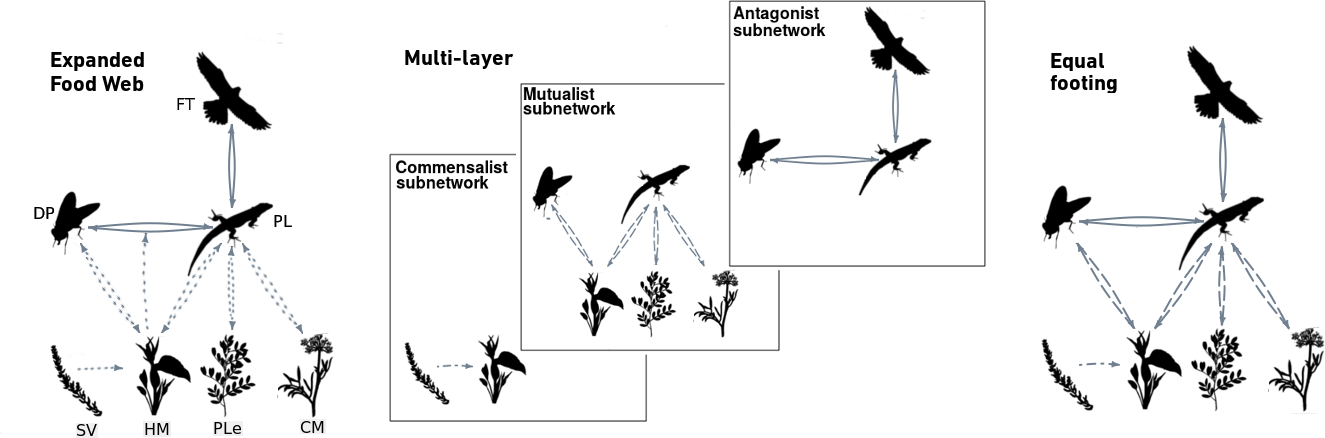
\includegraphics[width=\textwidth]{./Figures/chapter02/Fig_1.png}
\caption[Three approaches for multiple interactions networks]{\color{Gray} Three approaches for constructing and analyzing networks with multiple interaction types. In the first panel, solid lines represent trophic interactions, dotted lines non-trophic ones. Note that frugivory and pollination have both trophic and non-trophic components. In the second and third panels, solid lines represent antagonistic interactions, dashed lines mutualistic ones and dotted-dashed lines commensalistic ones. Data for building the network taken from the Aire Island community (see the Aire Island case study).}
\label{fig:fig2.1}
\end{figure}

\section*{Multilayer Networks}
The concept of networks formed by different types of interactions (edges, more generally, connecting two individual nodes of the network) was first developed in the first decades of the 20th century in the field of social sciences, for characterizing social interaction networks with different types of relationships between individuals. Nevertheless, it is only in the last few years that the idea has been properly defined mathematically, given a consistent terminology, and applied to a wide variety of research objectives in, for example, engineering, economical or social networks (see the reviews by \citealt{Boccaletti2014} and \citealt{Kivela2014} to learn more about the history, methodology and applications of the paradigm).

The basic principle is that nodes within a network can be linked in different ways or in different contexts, so that the overall network contains two or more layers that represent different link types or other aspects of variation. Nodes can be connected to nodes of the same layer (intra-layer links) or to nodes of different layers (inter-layer links). Such multidimensional object is called - in it most general definition - a multilayer network. An ecological community in which different species interact in a discrete number of ways is a very intuitive example of such a network \cite{Pilosof2017} each interaction type would constitute a different layer within the {}'interaction type{}' aspect, and other potential layering aspects could be time (i.e. the realization of the network in different sampling campaigns) or site (different sampling plots).

Mathematically, a multilayer network consists on a quadruplet  $M=\left(V_M,E_M,V,L\right)$  . Its elements are, first, a sequence of sets of elementary layers  $\left\{L_a\right\}_{a=1}^d$  , where  $d$  is the number of layering aspects. The full set of nodes of the network,  $V$  , does not include the information about which node belongs to which layer, so a further set of node-layer tuples encodes this information:  $V_m{\subseteq}V\times L_1\times {\cdots}\times L_d$  . These node-layer tuples, i.e. the instances of a node in a given layer, are called {}'state nodes{}'. Lastly,  $E_m{\subseteq}V_M\times V_M$  is the set of intra-layer and inter-layer links. This minimal definition is expanded in the reviews by \cite{Kivela2014} and \cite{Pilosof2017}. When designing multiple interactions networks,  $d{\geq}1$  , as at least the layering relative to interaction type will be present; also, links may be constrained to {}'diagonal coupling{}', i.e. the situation in which a node will only be connected to itself in different layers. Representations where layers are not interaction types but some other grouping of the community are also possible (Appendix 2.2). For modelling the dynamics of multilayer networks, any dynamical model representing species interactions may be used in which sub-networks are represented by sets of equations and, depending on the design, auxiliary equations may be used to connect the different state nodes of a given entity, or state nodes of different entities in different layers. The inter-layer links of a multilayer network make this framework particularly versatile, as these may represent any kind of relationship between layers (see \cref{fig:figApp2.2.3} for a definition of the different types of links in multilayer networks, and their matrix representation). For example, a link coupling the same plant species in pollination and herbivory sub-networks may represent the effect that consumption of reproductive organs by herbivores has in the interactions between the plant and its pollinators. Inter-layer links may also represent a coupling between layers with different temporal or spatial scales, thereby explicitly accounting for the temporal or spatial dimension of the networks. Note that this framework may accommodate networks with markedly different structures. For example, networks where virtually all links are intra-layer and the opposite, networks in which virtually all links are inter-layer, are both multilayer networks; also, networks whose nodes are present in every layer or in just one of them can fall under this framework.

Multilayer networks have been explored in a few studies of multiple interactions networks (Table \ref{tab:table1.1}), but their applicability in ecology goes far beyond these studies. For example, they have been successfully applied to reconstruct super (phylogenetic) trees \cite{vonHaeseler2012}, to study temporal and spatial variability in network structure, or to the analysis of ecological processes at different scales \cite{Pilosof2017} . Despite the potential of the multilayer framework for modelling ecological dynamics within and across layers, most studies listed in Table \ref{tab:table1.1} have only analysed static structural patterns, with the only exceptions being the studies by \cite{Stella2016}, who studied the dynamics of parasite spreading in multilayer ecological networks of varying structures, and by \cite{Gracia-Lazaro2018}, on the influence of inter-layer mutualistic interactions over layers of competitive interactions. In general, ecological studies on multilayer networks are starting to show that interactions other than predator-prey ones are also highly structured \citep{Melian2009,Kefi2015} and this topological structure has important consequences for different community properties \citep{Pocock2012, Evans2013a, Kefi2016a}.

As this approach has been developed mostly in theoretical physics and most reserachers in ecology may not be familiar with its terminology, a brief note is needed here. Following the definitions from \cite{Kivela2014}, a multilayer network is the most general object representing networks with multiple layering aspects and connections among layers. Although we focus on networks where the only layering aspect is interaction type and are diagonally-coupled, (termed `multiplex' networks or `edge-coloured multigraphs' in \citealt{Kivela2014}), we acknowledge that multiple interactions networks can also include other layering aspects and more complex patterns of inter-layer links. Therefore we adopt the more general term of multilayer networks in our review (Box 2). We will also use indistinctly the `layer' and `sub-network' terms to refer to a layer of specific interaction types in this framework.

\section*{Equal Footing Networks}

Regardless of the specific characteristics or vital rates of an organism potentially modified by a pairwise interaction, its effects can be summed up as influencing either (1) individual fitness, (2) population size, or (3) population growth rate \citep{Abrams1987}. This view of interactions as aggregating effects over general individual or population-level parameters is the conceptual basis behind {}'equal footing networks{}', with the main consequence that pairwise interactions of any type can be measured and compared {}'on equal footing'.

A minimal population dynamics model can be represented as in Eq. 1. The main difference with the expanded food webs is that here, trophic and non-trophic interactions influence the intrinsic growth rate through the interaction terms of the adjacency matrix  $\left[a_{\mathit{xy}}\right]$  , instead of being modelled through auxiliary equations 2-3. Therefore, the adjacency matrix may include all pairwise combinations \{(0,0),(0,+),(0,-),(+,-),(+,+),(-,-)\} (\cref{fig:figApp2.2.4} ).

Being a more general approach than expanded food webs, numerical models of equal footing networks are more scalable. Following Eq. 1, each species can be modelled by a single equation, and  $S^2+S$ parameters are required for a complete model of  $S$ species. This generality through the integration of fundamentally different interaction mechanisms in the adjacency matrix hinders the level of biological realism that can be achieved, in contrast with expanded food webs. By manipulating the signs of the adjacency matrix, different proportions of interaction types can be generated, but the effect of varying these proportions on community stability is an open question. \cite{Mougi2012} showed that, under certain conditions, local stability is enhanced for theoretical communities mixing antagonism and mutualism, as opposed to communities with a single interaction type. Their a priori conditions were that 1) mutualisms and antagonisms have, in total, the same effect over population growth rates and 2) for any species, the net effect of a given interaction decreases with increasing numbers of links of the same type. Two subsequent studies debated their conclusions: \citep{Suweis2014} stated that these conditions, and not the mixing of interaction types, were the factors that stabilized their models, whereas \citep{Kondoh2015} partially relaxed their initial assumptions and still found increasing stability with interaction mixing. Recently, the methodology developed in \citep{Mougi2012} has been expanded to assess the role of commensalism and amensalism \cite{Mougi2016a} and the potential switching of interactions \cite{Mougi2016b}, finding that separately accounting for these factors (unidirectional interactions and interaction switching) also increases local stability. The evaluation of equal footing networks through local stability analyses (for review see Table \ref{tab:table1.1}) is methodologically equivalent to the analysis of single-interaction networks. Hence, it is a natural approach for comparing networks of single and multiple interaction types without resorting to specific interaction mechanisms. In the studies already published (Table \ref{tab:table1.1}), different studies have considered different sets of interaction types and modelling assumptions, so that no integrative conclusions can be obtained at this point. Nevertheless, an emerging trend seems to be that networks with more than one interaction type and where different interactions are structured non-randomly are more locally stable than their single-interaction, non-structured counterparts.

The equal footing framework can be thought of as a particular type of multilayer network, in which the interaction layers are {}'flattened{}' in a single network, so that inter-layer links disappear, and each node is simultaneously affected by all interactions. \ This flattening is possible when three conditions are met: state nodes of the same node in the different layers of a multilayer network represent the same physical entity (as opposed to transportation networks, for example, where state nodes might represent bus or train stations of the same city), layers are diagonally-coupled, and all interactions in the different layers are expressed in the same units. This last condition is probably the most general, and in fact it represents our second criterion for distinguishing among frameworks. It allows the possibility of flattening multilayer networks in which there is link overlap among layers, as the overall effect will be a function of all layer-specific effects. We believe that these restrictive conditions, and the prevalence of equal footing networks in the theoretical studies listed in Table \ref{tab:table1.1}, merit the consideration of this framework as separated from the more general multilayer networks. The study by \cite{Melian2009} provides an example of a multilayer dataset flattened to an equal footing dynamic model.

\clearpage

\begin{small}
\begin{mdframed}
\subsection*{Box 1: Choosing a multiple interaction network methodology}
%\end{mdframed}
What constitutes a {}'realistic{}' representation of an ecological community? The answer is likely contingent on many factors, including the type of community being studied, the availability of empirical data and/or the ease to obtain it through observational or experimental studies. Although these factors, as well as research objectives and ecological assumptions, vary widely among studies, we propose a series of general guidelines for helping decide which multiple interactions framework is more appropriate for analyzing different types of data and questions (Fig. \ref{fig:fig2.1}).

The first dichotomy is whether the study involves structural and/or dynamical analyses (in this context, dynamical analyses refer to model-based projections of, at least, species abundances or biomass). In the first case, countless studies have analysed network structure based on lists of species and presence/absence of interactions between them. An excellent example of a structural analysis of a multiple interaction network is the comprehensive study of the Chilean rocky shore intertidal community by \cite{Kefi2015}. We suggest, for such analyses, arranging data according to the multilayer framework, which provides a versatile representation of the network and for which there is a well established, wide set of diagnostic metrics \citep{Pilosof2017}.

When values of biomass/abundance and interaction strengths are sampled or estimated (for example, based on allometric relationships, as in e.g. \cite{Kefi2016a}, community dynamics can be modelled. In these cases, the influence of the parameterization on the results obtained should be appropriately gauged against null models, but this topic is out of the scope of our study.

If interactions are classified in terms of their effect over a certain population parameter, either equal footing or multilayer networks are the appropriate modelling frameworks for analyzing dynamical systems. In this situation, choosing one approach over the other depends crucially on our second general criterion, i.e. the units in which interaction strengths are represented. Other factors may also play a role, for example the presence of multilink overlap (see case study), the complexity of inter-layer links, or whether the dynamics of single-interaction sub-networks may be of interest when considered as separate entities. Generalizing, if it is of any interest to consider interaction types separately (for example, if different interaction types are modelled through different functional forms and with different units) or there are complex inter-layer connections, multilayer networks should be used. If, on the other hand, the interest lies in the overall dynamics of the whole system, equal footing networks might be preferable.

The other branch of the flow chart in Fig. \ref{fig:box1.fig1} represents the situation where estimates of interaction strength are classified according to the mechanism they act upon. In this case, if the community consists of relatively few species or functional groups, each interaction can be modelled in detail, and the number of parameters might still be manageable: expanded food webs provide the most appropriate framework for such situations. Modelling the dynamics of a higher number of species, on the other hand, usually implies less mechanistic knowledge of the interactions within the community, and therefore interactions can be grouped in layers of a multilayer network that represent specific families of mechanisms. Notwithstanding these guidelines, as before, other factors may play a role (e.g. the inclusion of interaction modifiers, as in the case study). In all cases, selecting an appropriate framework will ultimately depend on the data at hand, the objectives of the study and the judgement and familiarity of the researchers with the different methodologies.

% within mdframed environments,another float environment does not work well
% so use custom captions of the memoir class
%\begin{figure}[h]
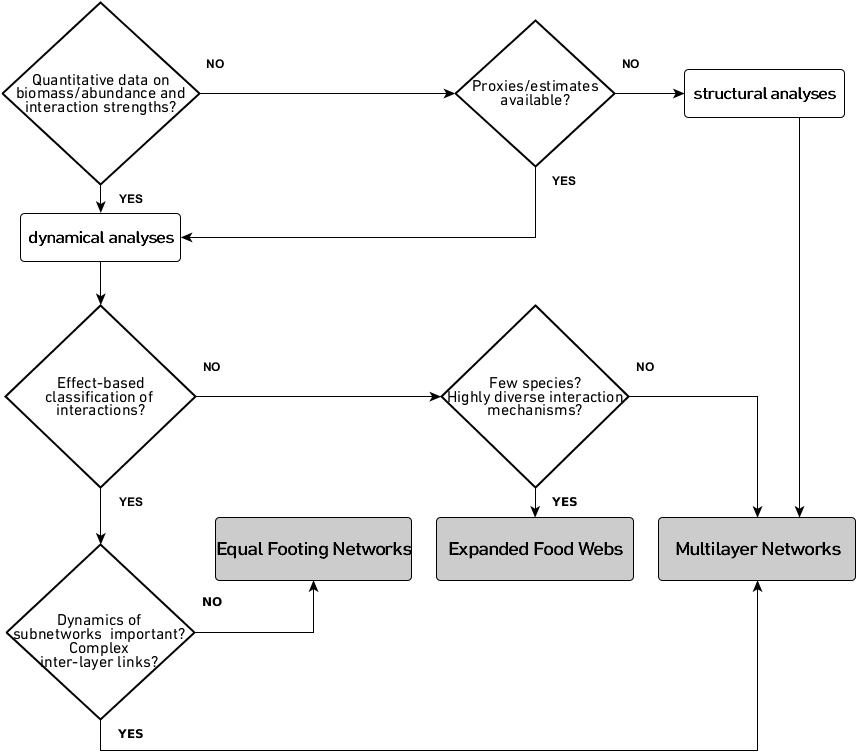
\includegraphics[width=.95\textwidth]{./Figures/chapter02/Box_1_Fig_1.png}
\figcaption[Choosing a multiple interaction network methodology]{\color{Gray} Diagram for choosing a multiple interaction network methodology, to be read starting from the upper left diamond box.}
%\caption}
\label{fig:box1.fig1}
%\end{figure}

\end{mdframed}
\end{small}

\section*{Acquisition and aggregation of empirical data}

Collecting data on the presence and strength of pairwise interactions in nature is notoriously difficult, even for the most easily observed interactions (Jordano 2016). It follows that interaction networks tend to be markedly under{}-sampled \citep{Chacoff2012}, and the proportion of type II errors, i.e. existing interactions that are not observed, is rarely known \citep{Olesen2011a, Morales-Castilla2015, Gravel2016}. In turn, quantifying the strength of observed interactions is also a long-standing challenge even for single interaction networks \citep{Berlow2004}. Several interaction strength indices have been developed by theoretical ecologists, but these are usually disconnected from the set of metrics obtained in field or manipulative studies \citep{Wootton2005}. Furthermore, very few pairwise interaction types have been extensively studied and their functional forms analysed (e.g. \citealt{Holland2002, Novak2008}), while the existence and/or dynamics of the vast majority of interactions in nature remain unknown. Thus, designing and implementing programs for collecting reliable data on multiple interaction types is presently one of the biggest challenges for community ecologists, up to the point that we are aware of just a handful of prominent examples in the literature. For example, \cite{Melian2009} aggregated data from several studies on pollination, seed dispersal and herbivory carried out between 1981-1984 in the Do\~nana Biological Reserve, in southern Spain. With that data, they constructed a network of 390 species and 798 interactions. Parasitic species and links, in addition to predator-prey interactions, were sampled by \cite{Hechinger2011} in food webs of three estuaries in the North American Pacific coast, in a dataset that included 314 species and 11270 interactions. In the study by \cite{Pocock2012}, several interaction types were concurrently sampled in different habitats of an agro{}-ecosystem in the UK, obtaining a network of 560 species and 1501 interactions. Finally, two networks of intertidal communities have been collected recently: \cite{Sander2015} obtained 1898 interactions between 110 taxa from the intertidal middle zone of Tatoosh Island based on observations and natural history of the species, and \cite{Kefi2015} took advantage of decades of work conducted on the marine rocky intertidal communities of the central Chilean coast to reconstruct its qualitative community network based on field observations and expert knowledge. Their network includes 104 species and 4754 interactions.

From these examples, one can distinguish two main strategies for constructing empirical multiple interactions networks: aggregating data from different sources of a given community in order to reconstruct the community network a posteriori (as in \citealt{Melian2009, Hechinger2011, Kefi2015} and \citealt{Sander2015}), or designing an integrated sampling program for a given set of previously defined interaction types, thus obtaining a realization of the network where all interactions are mostly co-occurring in space and time (as in \citealt{Pocock2012}). In the first approach, one may assemble information from studies conducted with different objectives and sampling methodologies and over different time periods, so that the aggregated network can potentially include a large fraction of the realized interactions, but these may or may not co-occur in time and/or space. Differential sampling efforts across studies will be unavoidable, and a posteriori analyses should be considered to minimize over or under-representation of certain clades and interactions. In the second approach, as fieldwork is likely to be conducted in tight time periods and in parallel for the different interaction types, sampling will potentially be more limited. On the other hand, this concurrent sampling is a more realistic snapshot of the co-occurring interactions in the sampling period, and importantly, fieldwork can be designed a priori to assign a near-homogeneous effort to different interaction types (but a posteriori corrections such as sample-based rarefaction are also advised; see \citealt{Pocock2012} and references therein). A non-exhaustive list of factors to account for the design of field campaigns is provided in Table \ref{tab:table1.2}, but a more comprehensive analysis of sampling strategies for multiple interactions networks is needed.

\begin{table} \footnotesize
\caption[Sampling of multiple interaction types]{\color{Gray}List of factors to consider in the design of sampling campaigns for multiple interaction types. These factors are general and independent from the framework chosen to represent the obtained network.}\label{tab:table1.2}
\begin{tabularx}{\textwidth}{p{2cm} X}
\hline
Factor & Examples of relevant questions\\
\hline
Temporal scale &
Single sampling campaign or periodic samples? What is the time scale of the interactions to be sampled? Are all/certain interaction types expected to vary along the sampling period?\\

Spatial scale &
What is the spatial scale of the interactions to be sampled? Are all/certain interaction types expected to vary spatially?\\

Habitat type(s) &
How many habitat types will be sampled? How does sampling effort vary across habitats? Which interaction types are expected to be prevalent in each habitat type?\\

Interaction types &
Which interaction types are expected to be sampled? Which sampling methodologies are applied to capture them? How does the proportion of forbidden links vary among interaction types?\\

Field and experimental observations &
Are experimental observations needed for observing specific interaction types (e.g. for estimating the prevalence of parasitism, or the number of flowers visited by a given pollinator)? How is effort distributed among field and experimental observations?\\

Natural history of species &
Do species in the community have varying activity periods or phenologies? Are there significant differences in mobility, behaviour, and other traits relevant to the probability of observing an interaction?\\

Movement capacity &
Will network include permanent species or also transient ones? How is a permanent species defined?\\
\hline

\end{tabularx}

\end{table}

Regarding the key issue of estimating empirical interaction strengths, it is often necessary to conduct manipulative experiments for obtaining reliable functional forms and interaction strength coefficients. Such experiments, however, are very context and clade-specific, and usually pose increased costs and logistical difficulties over field observations. For these reasons, a growing line of research is being developed for, given minimal information, inferring the presence \citep{Morales-Castilla2015, Deyle2016} and strength \citep{Novak2008, Berlow2009, Vazquez2012} of biotic interactions. Specifically, an interaction strength proxy that may be applicable to different types of interactions is the frequency of occurrence of an interaction. \cite{Poisot2015} proposed a general framework for integrating dynamic interaction strengths in dynamical models, taking into account the long-held idea that the net impact of a species over another can be described as a function of two components: the frequency of interaction and the per interaction effect \citep{Vazquez2005}. Thereby, the relative role of density-mediated and trait-mediated effects on direct interactions can be explicitly analysed. So far, it has been hypothesized that the net impact of mutualistic plant-pollinator interactions can be approximated by their frequency for both sides of the interaction \citep{Vazquez2005,Vazquez2012} and, in addition, that the asymmetry among interaction strengths is well explained in some cases solely by species' relative abundances (for quantitative bipartite networks, as in \citealt{Vazquez2007}). These ideas converge towards a unified neutral view of ecological interactions: interactions can be approximated as being the result of random encounters among individuals, whose probability is mediated by the relative abundances of the populations involved \citep{Araujo2014, Canard2012, Canard2014, Cazelles2016}. The frequency of interactions will naturally equal the net impact of a population over another, since per capita interaction strength will not vary with other factors (traits, environmental conditions). Further research is needed to test the robustness of (1) species abundance as a proxy for interaction frequency, and (2) interaction frequency as a proxy for interaction strength.

\begin{mdframed}
\begin{small}

\subsection*{Box 2: Definitions of key terms}

The approach used for classifying interactions does not only have methodological consequences: it is above all constrained by the very definition of interaction. Hence, it is important to be clear and explicit about the definitions used.

The ones we use in this study for direct and indirect interactions are taken directly from \cite{Abrams1987}. These definitions can be applied both to effect-based and mechanism-based classifications, and though we define indirect interactions for completeness, we mainly focus on direct interactions.

For effect-based classifications, existing definitions are complete, as they cover the full spectrum of possible combinations of interactions in what can be described as the biotic interaction space \citep{Araujo2014}. New terms have been introduced with time, e.g. expanding the definition of (+,-) interactions originally described as being mainly characterized by predation to, first, contramensalism \citep{Arthur1989} and later, antagonism \citep{Sousa1993}.

Within mechanism-based classifications the situation is somewhat more convoluted. In such studies, it is commonplace to study trophic and non-trophic interactions separately. Although defining these terms is apparently trivial, we have encountered very different implicit meanings of what constitutes a non-trophic interaction in the literature. For example, in the studies by \cite{Arditi2005} and \cite{Goudard2008}, non-trophic interactions are defined as modifiers of trophic interactions. \cite{Prasad2010} consider non-trophic interactions to be `driven by one species changing the behaviour but not the density of another species'. Finally, \cite{Kefi2012} interprets non-trophic interactions as being all other interactions than feeding ones, including the non-trophic components of pairwise interactions such as pollination or frugivory. We adopt the latter definition, as it more clearly fits within a simple generalizable framework, although it requires certain interactions to be split in their trophic and non-trophic components. Lastly, effect-based and mechanism-based classifications need not be mutually exclusive \citep{Abrams1987}: it is common for effect-based interaction classes to be divided according to specific ecological mechanisms, e.g. mutualisms can be divided by considering whether there is a trophic component in them or not, etc.

\begin{description}
\item[Interaction] A change in some characteristic of a population mediated by properties or actions by individuals of other population.

\item[Direct interaction] Interaction in which the effect occurs either through direct physical contact or through a third set of entities produced by one of the two interactors.

\item[Indirect interaction] Interaction in which the effect occurs as a result of other effects produced by one interactor on some population property of a third set of entities; and the third set of entities is not produced by any of the interactors.

\item[Trophic interaction] In the context of mechanism-based classifications, an interaction (or component of one) that involves direct exchange of energy (biomass) between the two individuals.

\item[Non-trophic interaction] In the context of mechanism-based classifications, an interaction (or component of one) that does not involve exchange of energy (biomass) between the two interacting individuals.

\item[Single-interaction network] Ecological network in which one interaction type is considered. Classic examples are food webs or plant-pollinator networks.

\item[Multiple interaction network] Ecological network with more than one interaction type. This umbrella term includes any topology and/or classification of interactions.

\item[Expanded food web] Multiple interaction network in which consumer-resource interactions form the basic structure of the network. Other interactions are termed ``non-trophic'' interactions and may affect any parameter of the dynamic model.

\item[Multilayer network] Network with different types of connections between nodes. In an ecological context, different network layers commonly represent different interaction types. If there is only one layering aspect and nodes are diagonally-coupled, that type of multilayer network is termed multiplex.

\item[Equal footing network] Multiple interaction network in which all interaction types are expressed in the same units, i.e. influence the same parameter of the dynamic model.

\end{description}
\end{small}
\end{mdframed}

\section*{The Aire Island case study}

The expanded food web, multilayer and equal footing frameworks for building multiple interactions networks offer complementary insights for the study of ecological communities, and each one is best suited to different types of studies and objectives (Box 1). Here, to demonstrate the diversity of ecological questions that can be addressed with multiple interactions networks, we analyse an empirical community under the lenses of each one of the approaches described. Specifically, we ask:

\begin{enumerate}
\item what is the influence of non-trophic interactions on the local abundances of all species? (expanded food web approach);
\item which species serve as ``hubs'' for linking species through interaction sub-networks and in the overall network? (multilayer network approach);
\item does the strength of different interaction types influences local community stability?(equal footing approach).
\end{enumerate}

The community examined is located on the Aire Island, a small islet located SE off the coast of Menorca (Balearic Islands, Spain) with an area of around 342500 m{\texttwosuperior}. Almost the entire surface of this relatively flat islet is exposed to the effect of the sea. Therefore, most vegetation is halophilous (i.e. thrives in saline environments) except in areas sheltered from wind and sea, where typical Mediterranean species appear, such as Pistacia lentiscus \citep{Perez-Mellado2006}. Our examples are based on a subset of the ecological community of this islet.

A remarkable set of interactions has been unveiled in the Aire Island between the dead horse arum (\textit{Helicodiceros muscivorus}), its associated insect pollinators (Diptera, genus \textit{Calliphora} and \textit{Lucilia}), and the Balearic lizard, \textit{Podarcis lilfordi}. The Balearic lizard is an omnivorous lacertid of medium size, endemic to the Balearic Islands. It has been shown to bask on the spathe of \textit{Helicodiceros muscivorus} {}' flowers, and to feed on the pollinating flies attracted by the intense odour produced by the plant. In addition to this negative effect of \textit{Podarcis lilfordi} on \textit{Helicodiceros muscivorus} through consumption of potential pollinators, it is itself an effective seed disperser of the plant: \textit{Podarcis lilfordi} consumes ripe fruits of \textit{Helicodiceros muscivorus} routinely, and seeds dispersed by the lizard show a significantly higher probability of germination than non-consumed seeds \citep{Perez-Mellado2006}. \textit{Podarcis lilfordi} is also an effective pollinator of other species at Aire Island. Particularly, high loads of pollen from \textit{Pistacia lentiscus} and \textit{Crithmum maritimum} have been found in lizard's bodies in previous studies on the same community \citep{Perez-Mellado2000}. Due to the scarcity of natural predators, \textit{Podarcis lilfordi} reaches high densities in the islet \citep{Perez-Mellado2008}. Its main predator is probably the Eurasian Kestrel (\textit{Falco tinnunculus}), that does not nest on the islet but visits it frequently. Lastly, the appearance of \textit{Helicodiceros muscivorus} is related to the percentage of soil covered by \textit{Suaeda Vera}, an hallophylous shrub of the Chenopodiaceae family, suggesting facilitation by the shrub on the development of \textit{Helicodiceros muscivorus} \citep{Perez-Mellado2006}. The interaction network formed by these 7 species (or guild, in the case of the Diptera) spans 3 trophic levels, and includes antagonistic, mutualistic and commensalistic interactions. In the following equations and figures, $S$ refers to the whole set of species, and species are denoted by their initials or silhouettes. When available, we use empirical data for parameter estimates. Whenever empirically derived estimates are unavailable, as these examples are only to illustrate the approaches, we assign values based on our judgements of plausibility.

\subsection*{Expanded food webs: Influence of non-trophic interactions in equilibrium abundances}

The main strength of the expanded food webs is the inclusion of detailed, mechanistic, non-trophic interactions in the general food web structure. We investigated their influence in the resulting abundance patterns of the community, compared to a standard food web model.

The continuous-time model for the expanded food web considers only three ecological processes: growth, mortality, and pairwise interactions, which can be trophic or non-trophic. Trophic interactions can, themselves, be modified by the presence of a third species. The main equations are of the form:

\begin{equation} \label{eq:2.4}
\frac{\mathit{dN}_x}{\mathit{dt}}=r_xN_x-m_xN_x^2+\sum _{y{\in}S,y{\neq}x}a_{\mathit{xy}}N_xN_y
\end{equation}

where  $r_x$  is the short-term per capita growth rate,  $m_x$ is the per capita mortality rate (that, multiplied by  $N_x^2$  , acts as a self-limitation term) and  $a_{\mathit{xy}}$  are the pairwise trophic interaction coefficients (the partial derivative of the per capita growth rate of species  $x$  with respect to the density of species  $y$  ).

Several non-trophic interactions are included on top of this general structure, affecting either  $r_x$ ,  $m_x$ or  $a_{\mathit{xy}}$ . As an example, the modification of the mortality rate is modelled with a saturating function \citep{Kefi2012}

\begin{equation} \label{eq:2.5}
m_x\left(N_y\right)=\frac{m_x^{\mathit{NTI}}N_y+m_x^0N_y^0}{N_y+N_y^0}
\end{equation}

The function varies between a basal value $m_x^0$ when $N_y=0$ , i.e. in the absence of non-trophic interactions, and  $m_x^{\mathit{NTI}}$ when the non-trophic interaction is highest. The same equation was used to model non-trophic interactions influencing the other parameters of Eq. 6 (growth rates  $r_x$ and interaction coefficients  $a_{\mathit{xy}}$ ). For modelling the Aire Island community, we assumed that (1) all mutualistic interactions positively affect short-term growth rates, i.e. $r_x^{\mathit{NTI}}>r_x^0$ for \textit{Helicodiceros muscivorus}, \textit{Podarcis lilfordi}, Diptera, \textit{Pistacia lentiscus} and \textit{Crithmum maritimum}; (2) the presence of \textit{Suaeda vera} increases the survival probability of \textit{Helicodiceros muscivorus} seedlings by providing a favorable microhabitat, thus decreasing the mortality rate of the facilitated plant, i.e. $m_{\mathit{HM}}^{\mathit{NTI}}<m_{\mathit{HM}}^0$ ; and (3) increases in abundance of \textit{Helicodiceros muscivorus} increased the magnitude of the predator-prey interaction between \textit{Podarcis lilfordi} and the Diptera species, i.e. $a_{\mathit{PL},\mathit{DP}}^{\mathit{NTI}}>a_{\mathit{PL},\mathit{DP}}^0$ and $a_{\mathit{DP},\mathit{PL}}^{\mathit{NTI}}<a_{\mathit{DP},\mathit{PL}}^0$.

The complete parameterizations of the expanded food web model and the equal footing model are included in Appendix 2.1. We found significant differences in abundances at equilibrium for all species except \textit{Suaeda vera}, depending on the set of interactions considered (Fig. \ref{fig:fig2.2}). We define equilibrium as the steady state reached after a sufficient number of time steps (2500 in our case). Non-trophic interactions in the Aire Island community are all positive, and accordingly, all populations increase in equilibrium abundance when engaging in non-trophic interactions. The only organism that conceivably could be negatively affected by the inclusion of non-trophic interactions are the Diptera, given that the magnitude of the \textit{Podarcis lilfordi} - Diptera antagonism is enhanced by higher abundance of \textit{Helicodiceros muscivorus}. With the parameterization chosen, however, the positive influence of the Diptera -- \textit{Helicodiceros muscivorus} mutualism outweighs this increase (Fig. \ref{fig:fig2.2}, note the increase in Diptera abundance when non-trophic interactions are considered). Note that this is the only approach in which we explicitly model the influence of \textit{Helicodiceros muscivorus} populations in the predator-prey interaction between the Diptera species and \textit{Podarcis lilfordi}.

\begin{figure}[ht]
\centering
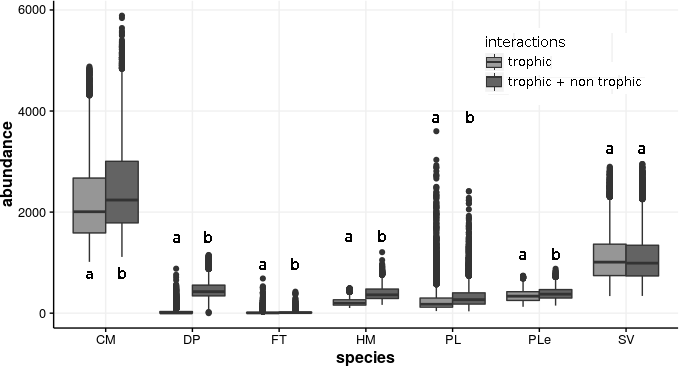
\includegraphics[width=\textwidth]{./Figures/chapter02/Fig_2.png}
\caption[Expanded Food Web analysis]{\color{Gray} Equilibrium abundances of the Aire Island community when considering trophic interactions, or trophic and non-trophic ones. Boxplots with different letters are significantly different according to Wilcoxon rank-sum tests (CM: W = 38176000, p {\textless} 0.05; DP: W = 63730000, p {\textless} 0.05; FT: W = 38512000, p {\textless} 0.05; HM: W = 57170000, p {\textless} 0.05; PL: W = 42005000, p {\textless} 0.05; PLe: W = 38454000, p {\textless} 0.05; SV: W = 31595000, p = 0.059).}
\label{fig:fig2.2}
\end{figure}

\subsection*{Multilayer networks: Importance of each species in structuring the network}

The role of the different species in structuring a given community has been extensively assessed for single-interaction networks \citep{Coux2016} and for multilayer networks in other fields \citep{Sole-ribalta2014,DeDomenico2015a}. For the multilayer framework, several metrics have been adapted directly from single-interaction networks and others have been defined taking into account the multidimensional nature of the multilayer approach \citep{DeDomenico2015a}. Among these novel metrics, the concept of multidegree is a multidimensional extension of the degree of a single-interaction network, that may help uncover important, well-connected species in each sub-network and in the overall structure. Here we calculate multidegrees as defined in \cite{Boccaletti2014}, where formal definitions are provided.

For understanding the concept of multidegrees, we first need to define the multilinks of the network. Multilinks (or multiedges) are links connecting two nodes in a combination of layers. For example, the Aire Island network has three interaction types. A multilink of the form (1,0,0) exists between two species if these species are connected in the first layer and not in the second or third one. One can see thus that the number of potential multilinks between any two species in a general network with  $M$  layers is  $2^M$  . The multidegrees  $m_x^i$ of species  $i$ are its number of multilinks of type  $x$, and its aggregation,  $m^i$  , is the overall multidegree as considered e.g. in \cite{Stella2016}.

Given three layers representing interaction types \{antagonism, commensalism, mutualism\}, the multilinks for the Aire Island network are:

\begin{equation*}
\begin{matrix}m_0=\{0,0,0\}\\m_1=\{0,0,1\}\\m_2=\{0,1,0\}\\m_3=\{0,1,1\}\\m_4=\{1,0,0\}\\m_5=\{1,0,1\}\\m_6=\{1,1,0\}\\m_7=\{1,1,1\}\end{matrix}
\end{equation*}

where  $m_0$ is the null multilink, representing the situation in which two species are not connected in any layer, and subsequently,  $m_7$ represents a multilink whereby two species are connected in the three layers. The number of shared multilinks between any two species can be represented by multi-adjacency matrices. The multi-adjacency matrices of the Aire Island community are:

\begin{equation*}
A^{m_0}=\begin{matrix}\text{ }\\\left.\phantom{\begin{matrix}\mathit{FT}\\\mathit{PL}\\\mathit{DP}\\\mathit{HM}\\\mathit{SV}\\\mathit{PLe}\\\mathit{CM}\end{matrix}}\right(\end{matrix}\begin{matrix}\mathit{FT}&\mathit{PL}&\mathit{DP}&\mathit{HM}&\mathit{SV}&\mathit{PLe}&\mathit{CM}\\0&0&1&1&1&1&1\\0&0&0&0&1&0&0\\1&0&0&0&1&1&1\\1&0&0&0&0&1&1\\1&1&1&0&0&1&1\\1&0&1&1&1&0&1\\1&0&1&1&1&1&0\end{matrix}\begin{matrix}\text{ }\\\left)\phantom{\begin{matrix}\mathit{FT}\\\mathit{PL}\\\mathit{DP}\\\mathit{HM}\\\mathit{SV}\\\mathit{PLe}\\\mathit{CM}\end{matrix}}\right.\end{matrix}\begin{matrix}\text{ }\\\mathit{FT}\\\mathit{PL}\\\mathit{DP}\\\mathit{HM}\\\mathit{SV}\\\mathit{PLe}\\\mathit{CM}\end{matrix}
\end{equation*}

\bigskip

\begin{equation*}
A^{m_1}=\begin{matrix}\text{ }\\\left.\phantom{\begin{matrix}\mathit{FT}\\\mathit{PL}\\\mathit{DP}\\\mathit{HM}\\\mathit{SV}\\\mathit{PLe}\\\mathit{CM}\end{matrix}}\right(\end{matrix}\begin{matrix}\mathit{FT}&\mathit{PL}&\mathit{DP}&\mathit{HM}&\mathit{SV}&\mathit{PLe}&\mathit{CM}\\0&0&0&0&0&0&0\\0&0&0&1&0&1&1\\0&0&0&1&0&0&0\\0&1&1&0&0&0&0\\0&0&0&0&0&0&0\\0&1&0&0&0&0&0\\0&1&0&0&0&0&0\end{matrix}\begin{matrix}\text{ }\\\left)\phantom{\begin{matrix}\mathit{FT}\\\mathit{PL}\\\mathit{DP}\\\mathit{HM}\\\mathit{SV}\\\mathit{PLe}\\\mathit{CM}\end{matrix}}\right.\end{matrix}\begin{matrix}\text{ }\\\mathit{FT}\\\mathit{PL}\\\mathit{DP}\\\mathit{HM}\\\mathit{SV}\\\mathit{PLe}\\\mathit{CM}\end{matrix}
\end{equation*}

\bigskip

\begin{equation*}
A^{m_2}=\begin{matrix}\text{ }\\\left.\phantom{\begin{matrix}\mathit{FT}\\\mathit{PL}\\\mathit{DP}\\\mathit{HM}\\\mathit{SV}\\\mathit{PLe}\\\mathit{CM}\end{matrix}}\right(\end{matrix}\begin{matrix}\mathit{FT}&\mathit{PL}&\mathit{DP}&\mathit{HM}&\mathit{SV}&\mathit{PLe}&\mathit{CM}\\0&0&0&0&0&0&0\\0&0&0&0&0&0&0\\0&0&0&0&0&0&0\\0&0&0&0&1&0&0\\0&0&0&1&0&0&0\\0&0&0&0&0&0&0\\0&0&0&0&0&0&0\end{matrix}\begin{matrix}\text{ }\\\left)\phantom{\begin{matrix}\mathit{FT}\\\mathit{PL}\\\mathit{DP}\\\mathit{HM}\\\mathit{SV}\\\mathit{PLe}\\\mathit{CM}\end{matrix}}\right.\end{matrix}\begin{matrix}\text{ }\\\mathit{FT}\\\mathit{PL}\\\mathit{DP}\\\mathit{HM}\\\mathit{SV}\\\mathit{PLe}\\\mathit{CM}\end{matrix}
\end{equation*}

\bigskip

\begin{equation*}
A^{m_4}=\begin{matrix}\text{ }\\\left.\phantom{\begin{matrix}\mathit{FT}\\\mathit{PL}\\\mathit{DP}\\\mathit{HM}\\\mathit{SV}\\\mathit{PLe}\\\mathit{CM}\end{matrix}}\right(\end{matrix}\begin{matrix}\mathit{FT}&\mathit{PL}&\mathit{DP}&\mathit{HM}&\mathit{SV}&\mathit{PLe}&\mathit{CM}\\0&1&0&0&0&0&0\\1&0&1&0&0&0&0\\0&1&0&0&0&0&0\\0&0&0&0&0&0&0\\0&0&0&0&0&0&0\\0&0&0&0&0&0&0\\0&0&0&0&0&0&0\end{matrix}\begin{matrix}\text{ }\\\left)\phantom{\begin{matrix}\mathit{FT}\\\mathit{PL}\\\mathit{DP}\\\mathit{HM}\\\mathit{SV}\\\mathit{PLe}\\\mathit{CM}\end{matrix}}\right.\end{matrix}\begin{matrix}\text{ }\\\mathit{FT}\\\mathit{PL}\\\mathit{DP}\\\mathit{HM}\\\mathit{SV}\\\mathit{PLe}\\\mathit{CM}\end{matrix}
\end{equation*}

\bigskip

\begin{equation*}
A^{m_3}=A^{m_5}=A^{m_6}=A^{m_7}=0
\end{equation*}

The multidegrees of the seven species of the community are the number of multilinks incident to them (Table \ref{tab:table1.3}). These metrics show that \textit{Podarcis lilfordi} is the most connected species, overall and both in the mutualist and antagonist sub-networks. \textit{Helicodiceros muscivorus} and Diptera are the following species in multidegree, and their links also span two layers. All other species are represented only in one layer, and are only connected to \textit{Podarcis lilfordi}, inviting the interpretation that the Balearic lizard has a disproportionate importance in structuring the community. In our small community, these results are visually evident, but the multidegree concept can be very useful in highly populated networks, where the importance of different species across layers is not obvious from visual inspection of the data. Note that by decomposing the overall multidegree into the contributions of each multilink we are able to evaluate the potential link overlap of any pair of species in any combination of layers. In our simple example, however, there is no overlap, a reasonable assumption when considering an effect-based classification of interactions over a single population parameter, since the potential partial positive and negative effects of a species over another are aggregated in order to calculate the net effect and the associated interaction type. For example, looking again at the \textit{Podarcis} -- \textit{Helicodiceros} interaction, the net direct effect of the lizard over the plant could be decomposed in, at least, 1) a negative effect due to the consumption of fruits (i.e. the trophic part of the pairwise interaction), 2) another negative effect due to the predation of potential Diptera pollinators, 3) the positive effect on seed dispersal, and 4) a further positive effect on survival of seeds that have been dispersed by \textit{Podarcis lilfordi} as opposed to seeds that germinate naturally. In the absence of more detailed experiments, and as suggested by \cite{Perez-Mellado2006}, we considered the overall effect of \textit{Podarcis lilfordi} over \textit{Helicodiceros muscivorus} to be positive. Link overlap in interactions can be expected when two species interact in different ways, for example due to varying ecologies of life stages, and more generally when the temporal dimension is included in the analyses.

\begin{table} \small
\caption[Multidegrees of the Aire Island multilayer network]{\color{Gray}Multidegrees of the seven species of the Aire Island multilayer network. Note that the trivial $m_0$ multilink represents no connections, so it is not considered for calculating the overall multidegree $m$.}\label{tab:table1.3}
\begin{tabularx}{\textwidth}{p{4cm}XXXXXXXXX}
\hline
& $m_0$ & $m_1$ & $m_2$ & $m_3$ & $m_4$ & $m_5$ & $m_6$ & $m_7$ & $m$\\ \hline
Falco tinnunculus & 5 & 0 & 0 & 0 & 1 & 0 & 0 & 0 & 1\\
Podarcis lilfordi & 1 & 3 & 0 & 0 & 2 & 0 & 0 & 0 & 5\\
Diptera & 4 & 1 & 0 & 0 & 1 & 0 & 0 & 0 & 2\\
Helicodiceros \ muscivorus & 3 & 2 & 1 & 0 & 0 & 0 & 0 & 0 & 3\\
Suaeda vera & 5 & 0 & 1 & 0 & 0 & 0 & 0 & 0 & 1\\
Pistacia lentiscus & 5 & 1 & 0 & 0 & 0 & 0 & 0 & 0 & 1\\
Crithmum maritimum & 5 & 1 & 0 & 0 & 0 & 0 & 0 & 0 & 1\\ \hline
\end{tabularx}

\end{table}


\subsection*{Equal footing networks: Influence of the magnitude of mutualistic and antagonistic interactions on community stability}

For assessing the effect of the strength of different interaction types on the overall stability of the network, we modelled the community using the equal footing framework. We used the continuous-time logistic equations proposed by \cite{Garcia-Algarra2014}, in which all extrinsic effects -- environmental, biotic interactions -- fall on the intrinsic growth rate  $r_x$ :

\begin{equation} \label{eq:6}
\frac{\mathit{dN}_x}{\mathit{dt}}=r_xN_x
\end{equation}

where

\begin{equation} \label{eq:7}
r_x=r_x^0+\sum _{y{\in}S,y{\neq}x}a_{\mathit{xy}}N_y-\left(\beta _x+c_x\sum _{y{\in}S,y{\neq}x}a_{\mathit{xy}}N_y\right)N_x
\end{equation}

The rightmost term of Eq.9 represents the self-limitation term. In the absence of pairwise interactions, the parameter $\beta _x$ controls self-limitation, and $c_x$ is a proportionality constant. Pairwise interaction coefficients  $a_{\mathit{xy}}$ were assumed constant. For assessing the relative influence of different interaction types on community stability, we varied the relative magnitude of facilitative (commensalistic and mutualistic interactions) and antagonistic coefficients and analysed the resulting local stability patterns of the system by examining the sign of the leading eigenvalue of the associated Jacobian matrix (Fig. \ref{fig:fig2.3} and \cref{fig:figApp2.3.2} ).

Parameterizations with weak antagonistic interactions were virtually all stable (19991 out of 20000 replicates), regardless of the magnitude of facilitative interaction strength (Fig. \ref{fig:fig2.3}, groups a and b). Communities parameterized with strong antagonistic interactions (group c in Fig. \ref{fig:fig2.3}), on the other hand, were mostly unstable, with only 20 out of 10000 replicates having a leading eigenvalue {\textless} 0. All unstable communities were also unfeasible in that either key species went extinct or some species grew unbounded despite the self-limitation term of Eq. 9. Interaction strength magnitudes were chosen arbitrarily, in the absence of empirical data, but patterns were robust to variations of +- 2 orders of magnitude. Our results therefore suggest that increasing antagonist interaction strengths for this particular community would lead to instability. Bear in mind, though, that local stability analyses are only an approximation of ecological stability, as they only apply to closed systems in equilibrium. If accepting this assumption, local instability in the Aire Island community could be interpreted as being triggered by increased per capita antagonistic interaction strengths. These could appear, for example, if sexual dimorphism in \textit{Podarcis lilfordi} led to higher predation of females by birds, thus exerting a higher influence on population growth rate. This, however, does not seem to be case, since the only dimorphism reported in Aire Island is the slightly larger body size of males \citep{Perez-Mellado2000}; hence, no differential predation is expected.


\begin{figure}[!ht]
\centering
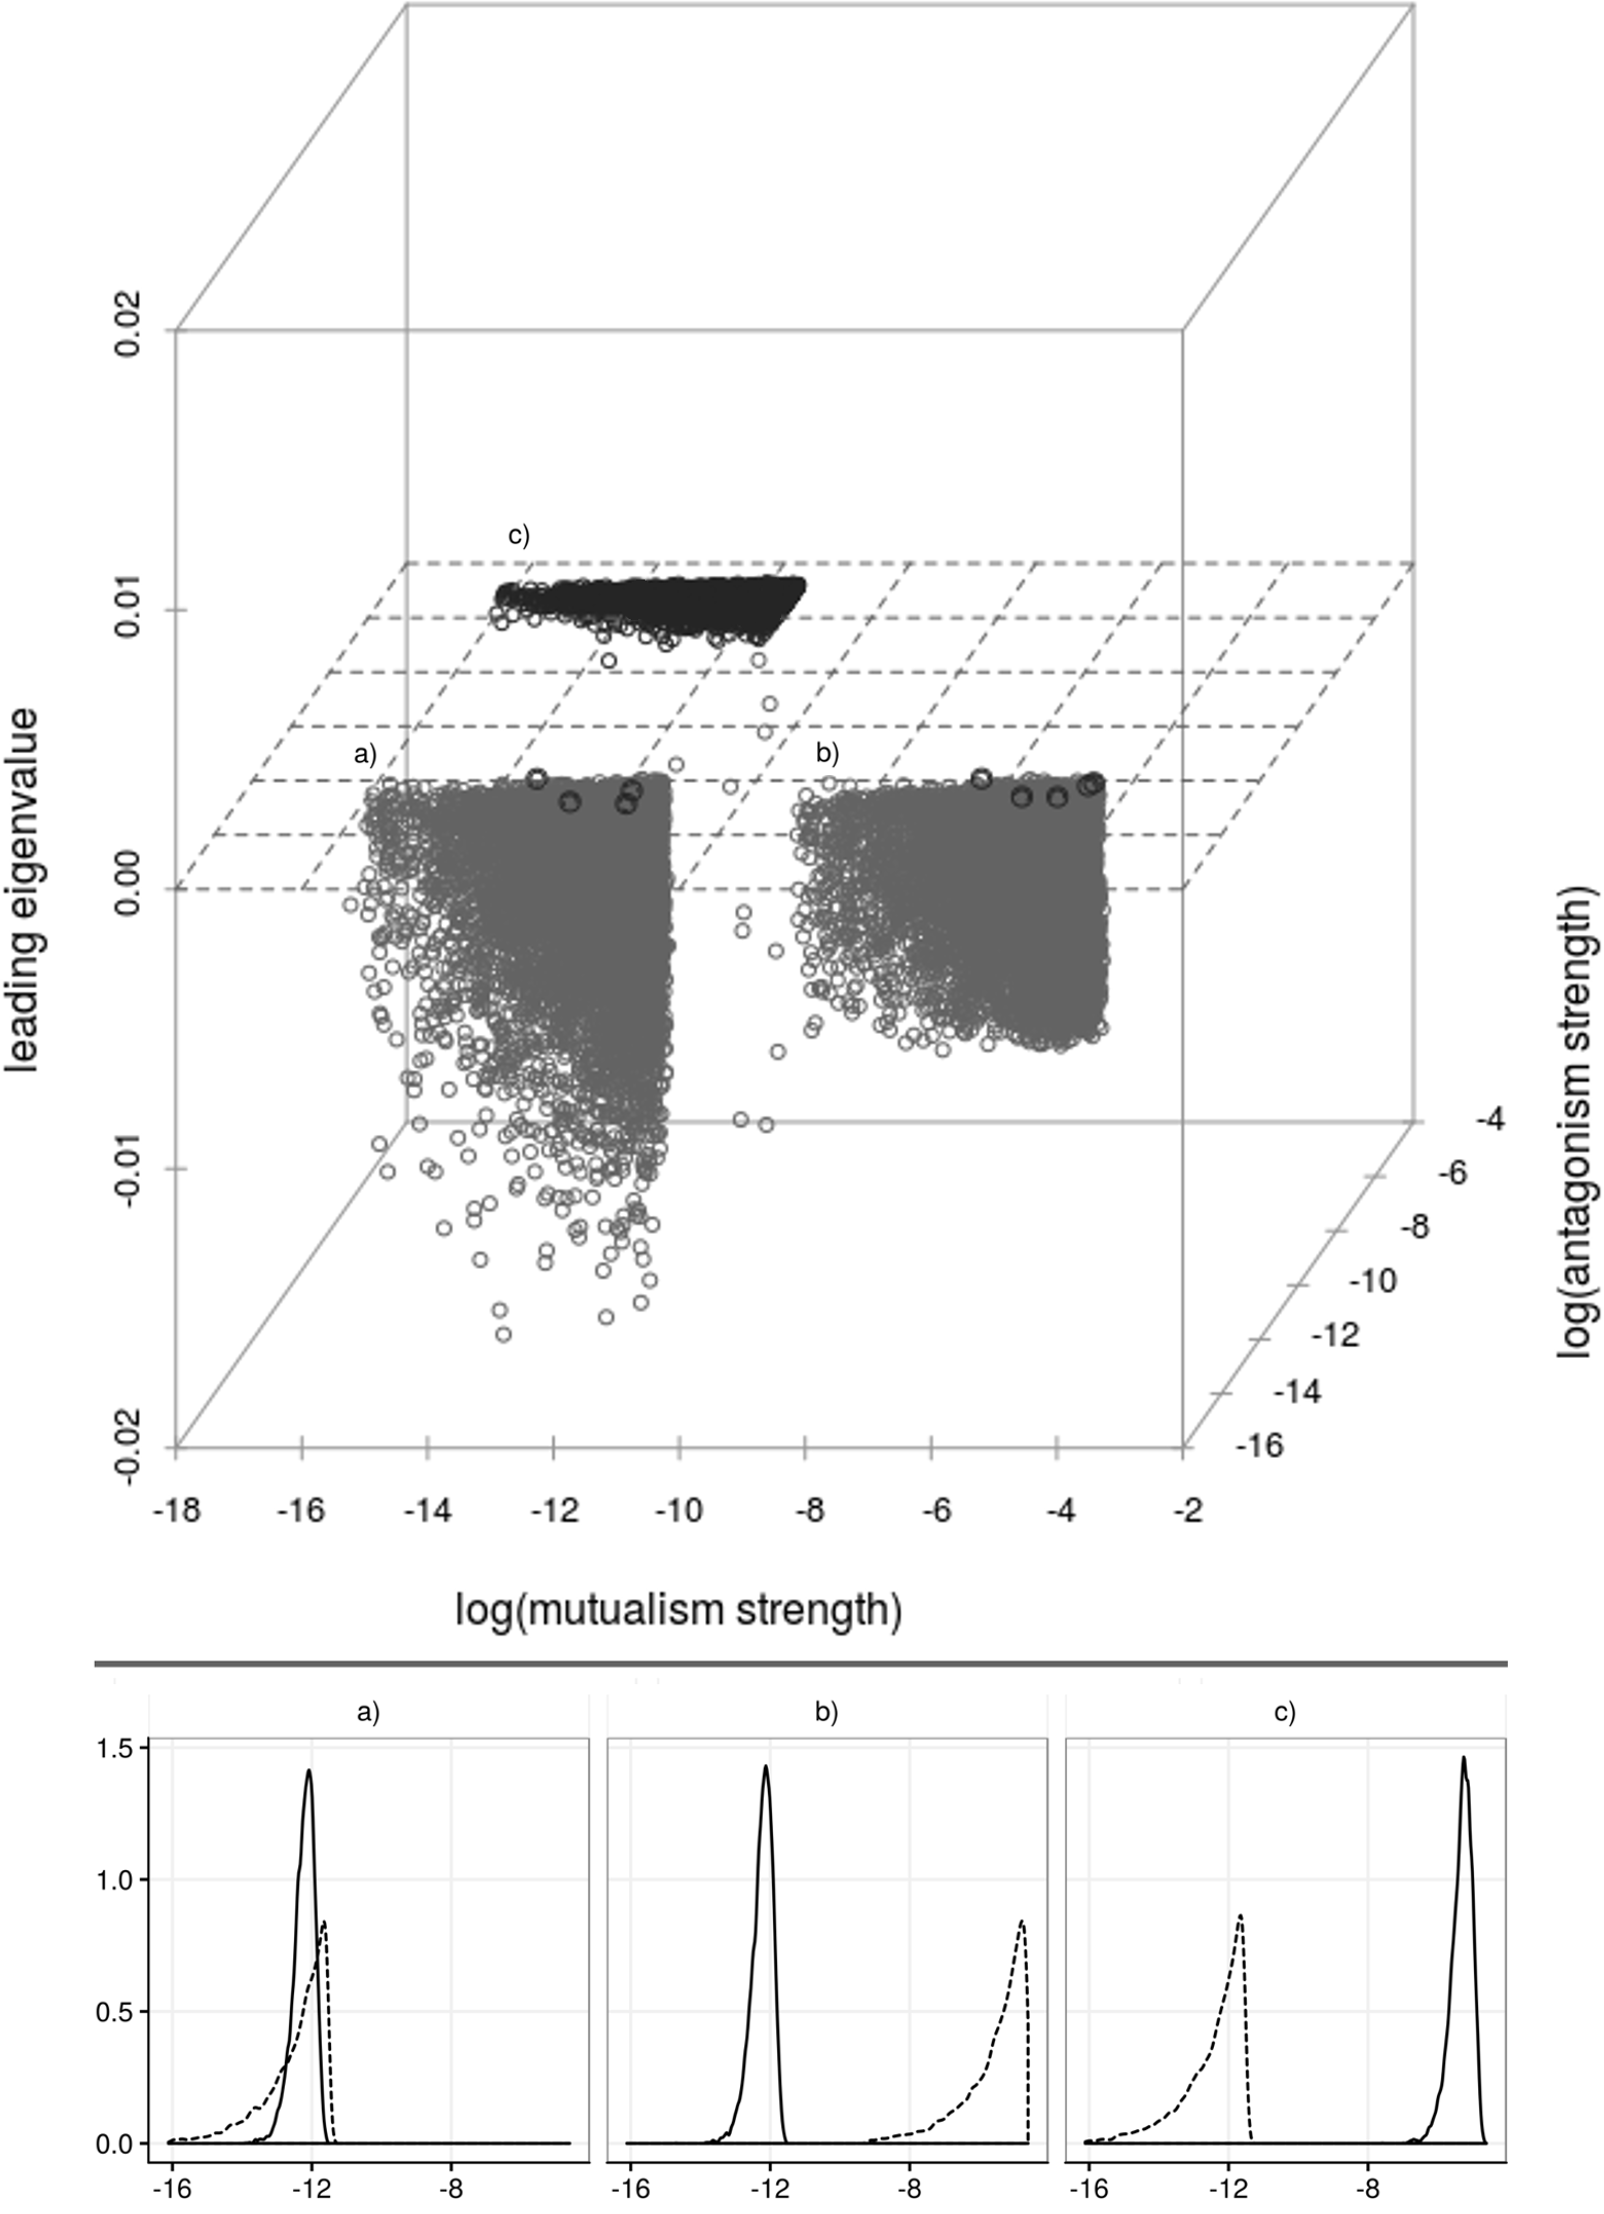
\includegraphics[width=.75\textwidth]{./Figures/chapter02/Fig_3.png}
\caption[Equal footing network analysis]{\color{Gray} Distribution of antagonistic and mutualistic interaction strengths and the leading eigenvalue of the resulting system. In the scatterplot, grey circles are systems with leading eigenvalue < 0, and black circles are systems with leading eigenvalue > 0. Group a) is the group of simulations with weak antagonistic and facilitative interactions; group b) are simulations with weak antagonistic and strong facilitative interactions; group c) are simulations with strong antagonistic and weak facilitative interactions. Within group c) only eigenvalue magnitudes close to 0 are shown, due to the extreme variability of the raw data (with values up to $10^99$ ). The rest of the data is shown in \cref{fig:figApp2.3.2} . For reference, a grid is drawn representing the z = 0 plane. Lower panels show the density distribution, for each group, of the logarithm of antagonist interaction strengths (solid lines) and the logarithm of facilitative interaction strengths (dashed lines).}
\label{fig:fig2.3}
\end{figure}


\section{Lessons from the case study}

In the Aire Island, the ecological community studied is structured around \textit{Podarcis lilfordi}, due to its high density and its key role as omnivorous feeder as well as seed disperser and pollinator of several plant species. This species and \textit{Helicodiceros muscivorus} are the ones most connected in the network, as shown by the multidegree analysis. Non-trophic interactions are key for correctly projecting population abundances, supporting empirical observations of the importance of facilitation between plant species \citep{Perez-Mellado2006} and effective seed dispersal by \textit{Podarcis lilfordi} \citep{Perez-Mellado2000}. We posit that the role of non-trophic interactions, as modelled in the expanded food web approach, will vary among communities and studies, but it is essential to integrate them in food web analyses, particularly for fine-scale and well-studied systems. Lastly, with the equal footing approach, we have shown that if we assume all interactions to influence intrinsic growth rates, the strength of antagonistic interactions controls the local stability of the network by potentially driving \textit{Podarcis lilfordi} or the Diptera pollinators to extinction. Specifically, even if no local extinctions occur, the variability on the \textit{Podarcis} abundances driven by an increase in antagonistic interaction strengths can destabilize the community, due to its central position on the network (as shown by the multidegree analysis). Positive interactions, in turn, can vary in magnitude without significant effects on local stability.

The results shown here, however, are merely to exemplify the application of the three methodologies on different ecological questions. Different methodologies evaluating the same problem may yield varying results; for example, equilibrium abundances of stable simulations obtained with the equal footing approach (\cref{fig:figApp2.3.1} ) vary significantly from those obtained with the expanded food webs (Fig. \ref{fig:fig2.2}). Choosing an appropriate formulation is not an exact science, as it involves a balance between available spatiotemporal data on species and interactions, natural history knowledge of the system, parsimony of the mathematical model, and objectives of the study (Box 1). In this particular community, in which the number of species is limited and the main interactions and mechanisms are relatively well-known, we advocate for more in-depth analyses based on expanded food webs, that may be parameterized with the results of manipulative studies of, e.g. localised removal of certain species or seed dispersal experiments for obtaining estimates of interaction strength.

\section{Network ecology moving forward}

Communities are comprised of individuals of different species interacting dynamically, and the wide variety of interactions any species engages in is key to its survival and thriving. Incorporating the effects of multiple interaction types in network analyses provides a more complete picture of community dynamics than relying on networks of a single interaction type. We have shown that frameworks for the study of multiple interactions networks are sufficiently mature and can accommodate a wide variety of research objectives and types of empirical data. We hope that the improved understanding of these frameworks, and the explicit recognition of their relative limitations and advantages, will lead to designing field studies that adequately capture the variety of interactions in communities, thus going beyond traditional approaches focusing on single interactions and often single clades. Questions in community ecology that remain unanswered can be addressed with a multiple interactions networks approach to the analysis of ecological communities. For example, we have little knowledge regarding the proportion among different types of interactions in real communities, whether this proportion is constant, whether it varies with any intrinsic or extrinsic factor, or whether it is related to community stability. Furthermore, it is unclear whether the trophic position of a species is related to the type of interactions it is more likely to be engaged in. Likewise, we have little knowledge of whether a species deemed important in a given sub-network will generally have such a role in sub-networks of other interaction types. Because observation of interaction strength in natural systems is extremely difficult to document, integration of empirical data and modelling frameworks requires that consistent interaction strength proxies be designed and tested. The neutral interactions hypothesis is a promising starting point for providing a metric applicable to all interaction types, but it needs to be tested for different communities and interaction types. On the other hand, the application of expanded food webs models to specific communities can trigger the design of manipulative studies to assess the functional forms and dynamics of non-trophic interactions, most of which remain unknown despite their importance.

These and other related questions are fundamental in order to understand the response of ecological communities to perturbations such as climate change or habitat loss. In summary, the development of theoretical models, such as the ones presented here, needs to be contrasted with multipe field or experimental studies for different community types.

%%************************************************
\chapter[Persistence and biotic interactions]{The effect of multiple biotic interaction types on species persistence}\label{ch:model}
%************************************************

\tikz[remember picture,overlay] \node[opacity=0.3,inner sep=0pt] at (current page.center){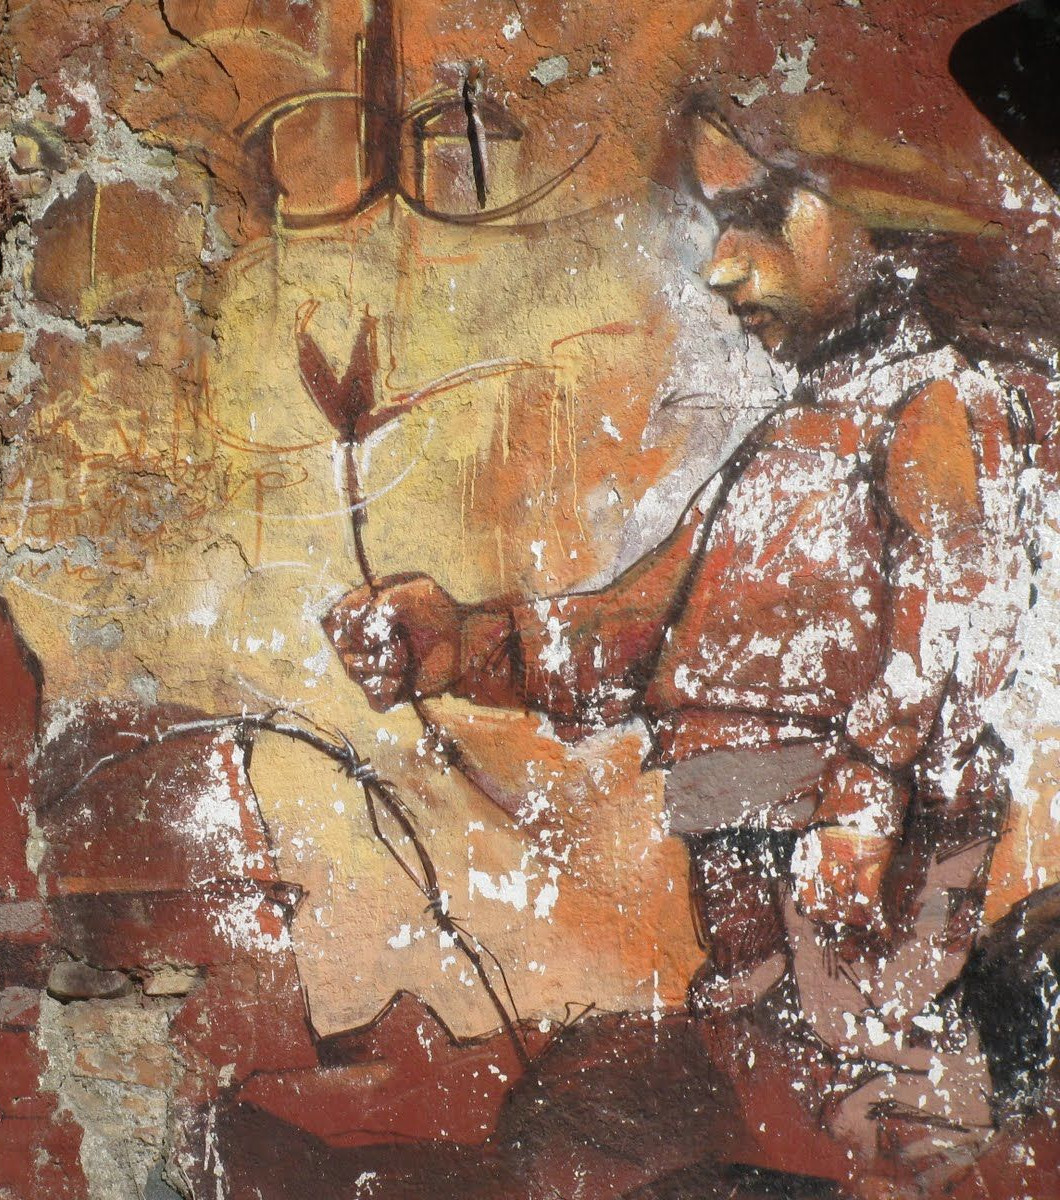
\includegraphics[width=\paperwidth,height=\paperheight]{./Figures/cover/n_pared_2.jpg}};
\clearpage

\section*{Abstract}
No species can persist in isolation from other species, but how biotic interactions affect species persistence is still a matter of inquiry. Is persistence more likely in communities with higher proportion of competing species, or in communities with more positive interactions? How do different components of community structure mediate this relationship? We address these questions using a novel simulation framework that generates realistic communities with varying numbers of species and different proportions of biotic interaction types within and across trophic levels. We show that when communities have fewer species, persistence is more likely if positive interactions—such as mutualism and commensalism—are prevalent. In species-rich communities, the disproportionate effect of positive interactions on persistence is diluted and different combinations of biotic interaction types can coexist without affecting persistence significantly. We present the first theoretical examination of how multiple-interaction networks with varying architectures relate to local species persistence, and provide insight about the underlying causes of stability in communities.

\section{Introduction}

Persistence of multicellular organisms depends on interactions with other organisms, whether they be in the form of energy intake, use of habitats created by other species, assistance in reproduction by directed dispersal of genetic material, or countless other examples \citep{Bascompte2007}. Ecological communities can be represented as networks, whereby species or guilds are nodes connected by links representing interactions \citep{Proulx2005}. Pairwise direct interactions can have positive, negative or neutral effects on the species involved, and this classification gives rise to five general types of interactions: amensalism (-,0), antagonism (+,-), commensalism (+,0), competition (-,-) and mutualism (+,+). Despite the wealth of empirical observations of biological interactions in nature, there still exists limited understanding of the frequency with which different types of biotic interactions occur in communities, and the consequences for community structure and functioning. For example, is the frequency of interaction types in communities related to overall persistence of species locally? Does the structure of the different interaction types play a role in increasing the odds of species persistence? Answering these and other questions has been hampered by difficulties in simultaneously sampling different interaction types in natural systems. Consequently, most studies have been based on observations of single interaction types within networks, which obviously has limited the ability to generalize beyond particular cases.

This fundamental gap in the understanding of ecological networks has been largely acknowledged \citep{Strauss2004, Agrawal2007, Ings2009, Fontaine2011}, and there is increasing evidence that accounting for different interaction types generates novel insights on the structure and dynamics of ecological communities \citep{Pilosof2017, Garcia-Callejas2018}.  Analyses of networks with multiple interaction types have already been applied, for example, to investigate the distribution of the different interaction types and its relationship with species traits \citep{Kefi2015,Kefi2016a} or the robustness of communities to local extinctions and habitat loss \citep{Pocock2012,Evans2013a}. Recent studies have also focused on investigating the relationship between the diversity of interaction types and several facets of community stability, often reaching different conclusions over this relationship. For example, it has been proposed that 1) mixing of interaction types generally increases local stability of model communities \citep{Mougi2012,Mougi2014,Kondoh2015}, 2) mixing of interaction types generally decreases local stability of model communities or increases the number of functional extinctions \citep{Suweis2014,Sellman2016}, or 3) structural factors of the different sub-networks enhance or decrease their stability \citep{Melian2009,Sauve2014,Sauve2016}. The conflicting results over this fundamental question can be explained by the sheer diversity of modeling assumptions, structural constraints, and varying sets of interaction types included in the studies. For example, several studies \citep{Melian2009,Sauve2014,Sauve2016} analyzed communities consisting of only antagonistic and mutualistic interactions in which a central group of species (usually plants) is the guild connecting the mutualistic (e.g. plant-pollinator) and antagonistic (e.g. plant-herbivore) networks. Other studies considered model communities with only basic rules about food web structure \citep{Mougi2012,Suweis2014}. A common feature of most studies is that, with the exception of \cite{Mougi2016a}, their models did not consider the five general interaction types concurrently. However, \cite{Mougi2016a} only analyzed random interaction matrices in his model, making his conclusions difficult to contrast with those of other studies that assumed stronger structural constraints. The role of species richness in mediating community stability also has been extensively studied in single-interaction networks, and analytical derivations have been produced for idealized conditions in mutualism-competitition networks \citep{Allesina2012}. In most cases, theory shows that increasing richness decreases local stability of random networks, but it is unclear how species richness mediates different facets of stability in networks with more complex structures and varying proportions of interaction types.

All in all, while approaches assessing the local stability of random interaction networks have important heuristic value \citep{Allesina2012,Allesina2015}, such randomly assembled networks lack key structural patterns found in real communities \citep{Jacquet2016}. Furthermore, local stability analyses have little concordance with non-equilibrium dynamics of real systems \citep{Pimm1982,Chen2001}, which limits their predictive ability. The equilibrium assumption is further ingrained in most interaction models by assuming that interactions occur with a constant strength coefficient. This assumption is widely used for convenience despite repeated claims against its realism \citep{Abrams1980,Abrams2001,Hernandez1998,Holland2009}. Here we address all the above-mentioned shortcomings and investigate whether the frequencies of the five biotic interaction types affect persistence of species in communities with varying species richness. We generate model networks informed by empirical observations on distributions of species abundances across trophic levels, link topology, and develop a measure of the impact that a species has over another based not on static interaction coefficients, but on species abundances and their associated frequency of interaction. With this model design, and by performing a comprehensive set of simulations, we ask the following questions: 1) Is species persistence affected by the frequency of the different interaction types in model communities? If so, does community richness mediate this relationship? 2) Which types of biotic interactions are more likely to be lost, as species go locally extinct? Lastly, given the unfeasibility of validating our predictions with empirical data, we indirectly test the validity of our model by asking: 3) does our model generates community-level patterns consistent with those of empirical networks?

\section{Methods}

We designed a dynamic network model accounting for the five possible types of pairwise interactions (antagonism, amensalism, commensalism, competition, and mutualism), whereby the impact of a species over another is characterized by the abundances of the species involved. Accounting for different interaction types meant that a trophic level distribution of species had to be specified a priori, as we expected different interaction types to be distributed unevenly across trophic levels. Furthermore, the modeling of pairwise interactions in our model is closely linked to the abundances of the interacting species, so we imposed non-random initial abundance values. In particular, we assembled our model communities with three assumptions:

1) The initial Species Abundance Distribution of the overall community follows a hollow curve.


2) The initial abundances of the different trophic levels vary with a power-law scaling.


3) The distribution of interaction types within and across trophic levels is non-random.


In the following sections, we describe these assumptions and the methodology for incorporating them in the community assembly process. Then, we specify the implementation of the dynamic interactions model and the simulations performed. The main response variable obtained from our simulations is the ratio of persistent species in our model networks. Thus, in the context of the present study, we define community persistence as the ratio between initial (denominator) and final (numerator) number of species in a simulated community. Persistence values can therefore range from 0 (all initial species have died out by the end of the simulation) to 1 (all species show positive abundances at the end of the simulation).

\subsection*{1) Abundance distribution of the overall community}

Each species within a model community was assigned an initial abundance by drawing random samples from a gambin distribution. The gambin is a distribution with a single free parameter that provides a similar or better fit to empirical SADs than classic choices such as the lognormal or the logseries \citep{Matthews2014a}. A value of $\alpha = 2$ was given to generate the initial SADs.

\subsection*{2) Abundance scaling across trophic levels}

Species were distributed among four trophic levels (a basal one consisting on primary producers and three consumer levels), which is a number commonly found in empirical communities \citep{Ulanowicz2014a}. Assignment of species into each trophic level was made following the findings of \cite{Hatton2015}, who showed that for herbivore-predator trophic guilds, biomass distribution follows a power law with exponent ~ 0.75. These authors generalized the scaling rule to the abundance of species at each trophic level since, for most predator-prey couplings, weak relationships between body mass and community biomass were found. As a starting working hypothesis for the simulations, we extended Hatton’s et al (2015) scaling rule to the four trophic levels considered.

\subsection*{3) Distribution of interaction types within communities }

The different types of biotic interactions are unlikely to be uniformly distributed in nature. Yet little is known regarding the varying proportion of interaction types within communities or trophic levels \citep{Dodds1997}, let alone about changes in such proportions across communities, or the effects of varying proportions of interaction types on mechanisms of community assembly.

A first step towards examining the frequency distribution of the different interaction types in a community with several discrete trophic levels is to consider the sign matrix of the community, $S$, assuming that interaction signs are kept constant within the spatial and temporal limits of the study, and with varying abundances. We hypothesize that the relative frequency of each interaction type in S will be influenced by the number of species in the different trophic levels, as different interaction types will have different probabilities of occurring among species belonging to the same or different trophic levels. In order to check this working hypothesis, we undertook an extensive survey of literature on biotic interactions and compiled the extent to which the five general interaction types (amensalism, antagonism, commensalism, competition, mutualism) are documented to occur between species of the same, adjacent, or non-adjacent trophic levels. Specifically, we performed a search in the Web of Science for studies published from 1991 to 2015, including the terms “ecology” AND “interaction” AND “interaction type” (see also \citealt{Morales-Castilla2015}). We reviewed studies documenting direct pairwise interactions and annotated the trophic level of the species involved. For competition, antagonism (predation OR herbivory), and mutualism, we included \textit{ca}. 100 papers. For commensalism and amensalism the list of suitable studies was more reduced (67 studies on commensalism and only 12 on amensalism). We constrained the results by discarding interactions involving microorganisms, fungi, parasites or parasitoids, owing to the overall difficulty of classifying these groups into clear cut trophic levels. The list of selected studies is available as online supplementary material in the published article, see section \textit{Chapter references} for the full reference. The resulting relative frequencies (Fig. \ref{fig:fig3.1}) were incorporated as a last constraint in the model in the form of probabilities of pairwise interactions taking place within a single trophic level, adjacent, or other trophic levels.

For estimating the number of links of each species, we followed the constant connectance hypothesis \citep{Martinez1992}. Thus, we assumed no variation in connectance levels with initial community size, imposing C = 0.5 for every simulation, where connectance is defined as the ratio between realized and potential interactions in the network. This value was chosen so that specific connectances of the different interaction types (see Appendix 3.4) ranged between 0.07 and 0.2, values consistent with empirical estimates of mutualistic and antagonistic connectance \citep{Thebault2010}.

With the probabilities of interaction occurrence across trophic levels (Fig. \ref{fig:fig3.1}) and connectance values of the network, we constructed the sign matrices of our model communities stochastically: for each link, first its interaction type is selected; second, the trophic levels affected by that interaction are chosen according to the probabilities of interaction occurrence; and third, the specific species are randomly chosen. This process ensures that, on average, sign matrices will reflect the probabilities of Fig. \ref{fig:fig3.1}, while allowing for an intrinsic component of variability in each particular matrix. The full community assembly process is explained in detail in Appendix 3.1.

\begin{figure}[!ht]
\centering
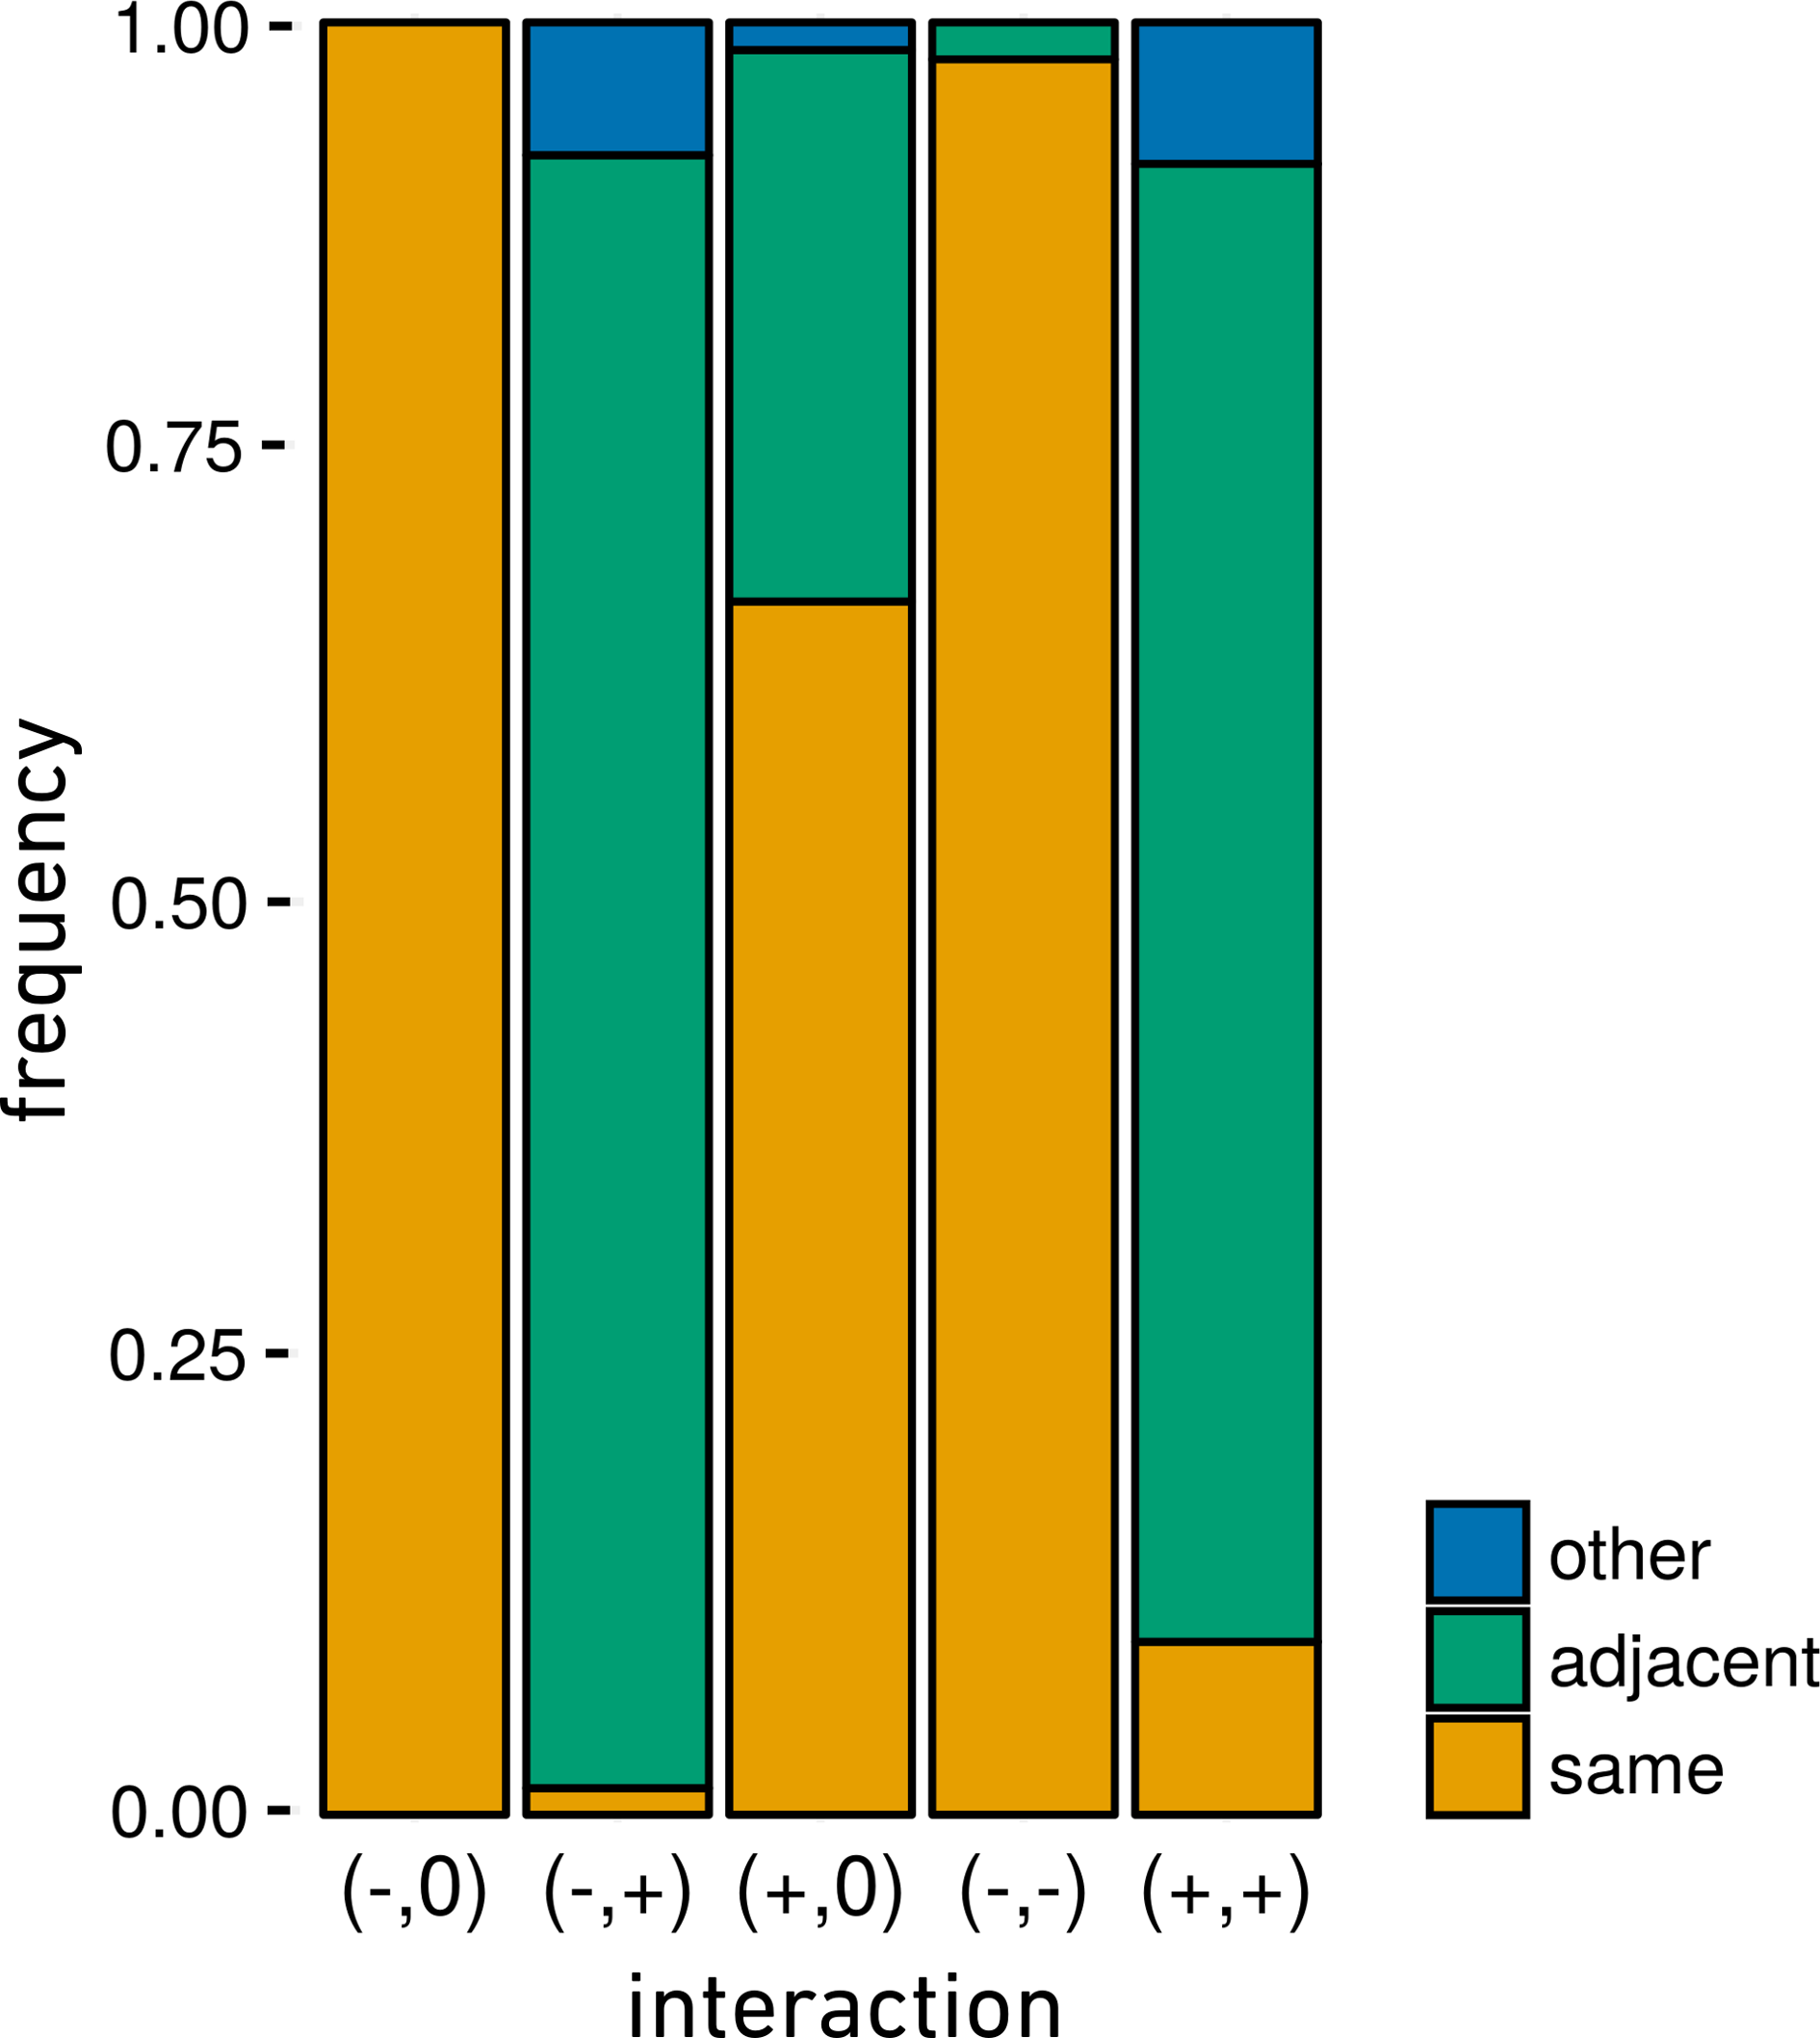
\includegraphics[width=.5\textwidth]{./Figures/chapter03/Fig_1.png}
\caption[Interaction occurrences across trophic levels]{\color{Gray} relative frequency of trophic levels involved in pairwise interactions for each interaction type. When the trophic level of the interacting species was not explicitly alluded to, we assumed that 1) species of the same taxonomic group belong to the same trophic level (e.g. isopods), 2) omnivory represents feeding on both “adjacent” and “other” trophic levels, 3) pollinators and seed dispersers are “adjacent” to plants. $N_{amensalism} = 12$, $N_{antagonism} = 135$ (123 of adjacent trophic levels, 10 of other, 2 of same), $N_{commensalism} = 65$ (44 of same trophic level, 20 of adjacent, 1 of other), $N_{competition} = 97$ (95 of same trophic level, 2 of adjacent), $N_{mutualism} = 113$ (94 of adjacent trophic levels, 11 of same, 9 of other).}
\label{fig:fig3.1}
\end{figure}

\subsection*{A framework for modeling dynamic interactions}

The realization and outcome of direct pairwise interactions is dependent on three classes of mechanisms \citep{Poisot2015}: First, the frequency of stochastic encounters of individuals mediated by their relative abundances. Second, the matching of traits between individuals that establish contact. Third, other factors such as environmental constraints or the influence of higher order interactions with other species. Hence, empirical measurements of interactions show a high degree of variability explained, partly, by density-dependent mechanisms \citep{Aizen2014}, by trait matching \citep{Santamaria2007} or by environmental factors \citep{Mazia2016,Poisot2017}. This inherent variability on both the sign and the strength of interactions has hardly been explored in community dynamic models, even if the assumption of static interaction sign and strength is known to be unrealistic \citep{Abrams1980,Abrams2001,Hernandez1998,Holland2009}. The importance of each mechanism in explaining observed patterns of interaction strengths is currently under debate. In plant-pollinator networks, for example, the net impact of a species over another is significantly related to the frequency of interaction \citep{Vazquez2005,Vazquez2012}, and to the abundances of the interacting species \citep{Vazquez2007}, but not in all cases. A neutral model of interactions can also reproduce structural patterns observed in empirical food webs \citep{Canard2012}. On the other hand, trait-matching has been shown to accurately reproduce network structure in different types of networks \citep{Eklof2013}, and also outperforms neutral interaction frequency for predicting network structure in some empirical networks \citep{Vizentin-Bugoni2014,Sazatornil2016}. However, another recent study showed that while abundances and traits can predict network structural patterns, they were not generally able to predict the realization of specific interactions in a plant-pollinator network \citep{Olito2014}. Finally, higher-order influences on interaction occurrence and strength, in particular environmental forcing, are a main focus of Stress Gradient Theory \citep{Maestre2009} and Environmental Stress Models \citep{Menge1987}, but an integration of these frameworks with the recent advances on multi-trophic, multiple interactions networks is still lacking.

We modeled the impact of a species over another by considering the first of these three mechanisms, i.e. the stochastic encounters between individuals of two populations driven by their abundances. This process is the only one that can be generalized to any interaction and community type without considering further, specific assumptions about trait distributions or the role of environmental covariates. Thus, in our modeling framework, the impact of a species over another is only dependent on the frequency of interaction between the two species, which in turn depends on their net abundances. As our approach is fundamentally different to that of models with static interaction strength coefficients, we refer to the interaction strength in our model as species impact (a population-level effect, \citealt{Vazquez2012}).

In formulating species impact, we followed \cite{Poisot2015} and considered it a product of interaction frequency by an interaction strength term:

\begin{equation} \label{eq:eq3.1}
I_{i,j} = IF_{i,j} * IS_{i,j}
\end{equation}

The $IF$ function derives the net frequency of interactions between two populations in a given time interval from their local abundances. We assume that (1) the maximum potential interaction frequency will equal the population density of the least abundant species, and (2) interaction frequency saturates asymptotically, as one or both abundances increase. It takes the form:

\begin{equation} \label{eq:eq3.2}
IF_{i,j} = min(N_i,N_j) \frac{1}{1 + e^{-a(max(N_{i},N_{j}) - x_0)}}
\end{equation}

The $a$ parameter adjusts the saturating behavior of the function (i.e. its steepness), so that a higher value of a implies that the $IF$ function saturates at lower abundances of both populations, i.e. interactions are comparatively more common. Parameter $x0$ indicates the abscissa of the midpoint for the logistic part of the function, and was kept for reference.

The $IS$ function (for interaction strength) models the sign and strength of per capita interactions of species $j$ over species $i$. This function was defined just as the sign of the pairwise interaction times a scaling factor for differentiating interaction types. For example, a scaling of 1 indicates that the maximum effect of species $j$ over species $i$ is of the same order of magnitude as the population growth rate. Therefore, we defined the $IS$ function simply as:

\begin{equation} \label{eq:eq3.3}
IS_{i,j} = s_{i,j} * k_t
\end{equation}

where $s_{i,j}$ is the sign of the effect of species $j$ over species $i$, and $k_t$ is the scaling factor for an interaction of type $t$.

We incorporated Eq. \ref{eq:eq3.1} to a population dynamics model based on the recent extensions to the logistic growth equation by \cite{Garcia-Algarra2014}. Their formulation averts a known divergent behavior of the r-k classic form of the logistic equation and is sufficiently simple while being able to reproduce the complexity of more elaborate models in terms of fixed points and stabillity of the dynamics. Consider a community of $n$ species. The model has the form:

\begin{equation} \label{eq:eq3.4}
\frac{dN_i}{dt} = r_i N_i
\end{equation}

whereby all extrinsic effects – environmental, biotic interactions – fall on the intrinsic growth rate $r_i$. This allows the comparison between the strength of different interactions, i.e. it is an example of an equal footing network \citep{Garcia-Callejas2018}. The effective growth rate is modeled as:

\begin{equation} \label{eq:eq3.5}
r_i=r_i^0+\sum_{j=1,j{\neq}i}^n I_{i,j} - (\alpha_i + c_i \sum_{j=1,j{\neq}i}^{n} I_{i,j})N_i
\end{equation}

where $r_{i}^{0}$ is the intrinsic growth rate, $\alpha_i$ is the friction term that regulates the asymptotic behavior of the function, $c_i$ is a proportionality constant, and $I_{i,j}$ is the impact function from Eq. \ref{eq:eq3.1}.

\subsection*{Simulations}

We generated theoretical communities with 20,40, and 60 initial numbers of species that corresponded to overall abundances of around 2395, 4640 and 6850 individuals, respectively. For each richness level, we defined six types of communities according to the frequency with which the different interaction types occurred: equal ratio type with relative frequency of 0.2 for every interaction type; and five types in which each of the interaction types was the most prevalent (with frequencies of 0.4 for the prevalent type and 0.15 for the others). We projected the dynamics of 1000 replicates for each of these combination of factors, ending up with $3*6*1000 = 18000$ simulated communities. For each replicate, aside from the inherent stochasticity of the assembly process, we drew the intrinsic growth rates and saturation terms of each species ($r_{i}^{0}$ and $\alpha_i$ from eq. \ref{eq:eq3.5}) randomly from an interval of potential values (\cref{tab:tableApp3.1.4}), ensuring that primary producers have intrinsic growth rates $r_{i}^{0} > 0$ and consumers $r_{i}^{0} < 0$. Introducing these stochastic components on the assembly process and parameterization enabled us to test the robustness of the model to small variations in its initial conditions. The full parameterization of the model, alongside with further details about its implementation and numerical solving, is given in Appendix 3.1. Preliminary tests showed that most simulated communities reached a stable abundance distribution after 2500 or less time steps but, conservatively, we ran our dynamic model for 5000 time steps. In order to be more confident on the time steps chosen, we also tested whether there were significant differences between the resulting persistence patterns after 5000 and 10000 time steps. As no significant differences were found, we considered 5000 time steps to be an appropriate time frame for our simulations.

We also performed additional simulations in order to test the influence of the imposed structural constraints in our results. In these simulations we relaxed, one by one, the three constraints of the community assembly process (see Appendix 3.3 for more details).

\section{Results}

\subsection*{Is species persistence influenced by the frequency of the different interaction types? If so, does community richness mediate this relationship? }

Model communities with a higher proportion of positive interactions (mutualism and, to a lesser extent, commensalism) tended to have higher species persistence than any other community type (Fig. \ref{fig:fig3.2}, results of statistical tests in \cref{tab:tableApp3.2.1} and \cref{tab:tableApp3.2.2}). The effect of positive interactions on persistence was strongest for species-poor communities, and decreased consistently as the numbers of species in the communities increased. Although average species persistence converged to around 88\% as richness increased, there was significant variation between the persistence of species belonging to the different trophic levels (\cref{fig:figApp3.2.1}): in communities with low initial richness, the second and third trophic levels saw more extinctions than the first, while species on the fourth trophic level did not show a uniform behavior, and were more dependent on variations in the relative frequency of interaction types. This general pattern was reversed in more speciose communities, in which species of all higher trophic levels showed more persistence than the basal ones, for all community types.

Supplementary simulations (Appendix 3.3) showed that persistence values are further influenced by the community structural patterns imposed. The removal of both the abundance scaling across trophic levels and the distribution of interaction types across trophic levels had a significant negative effect on persistence. Sampling species abundances from a uniform SAD instead of a skewed one, on the other hand, increased overall persistence.

\begin{figure}[!ht]
\centering
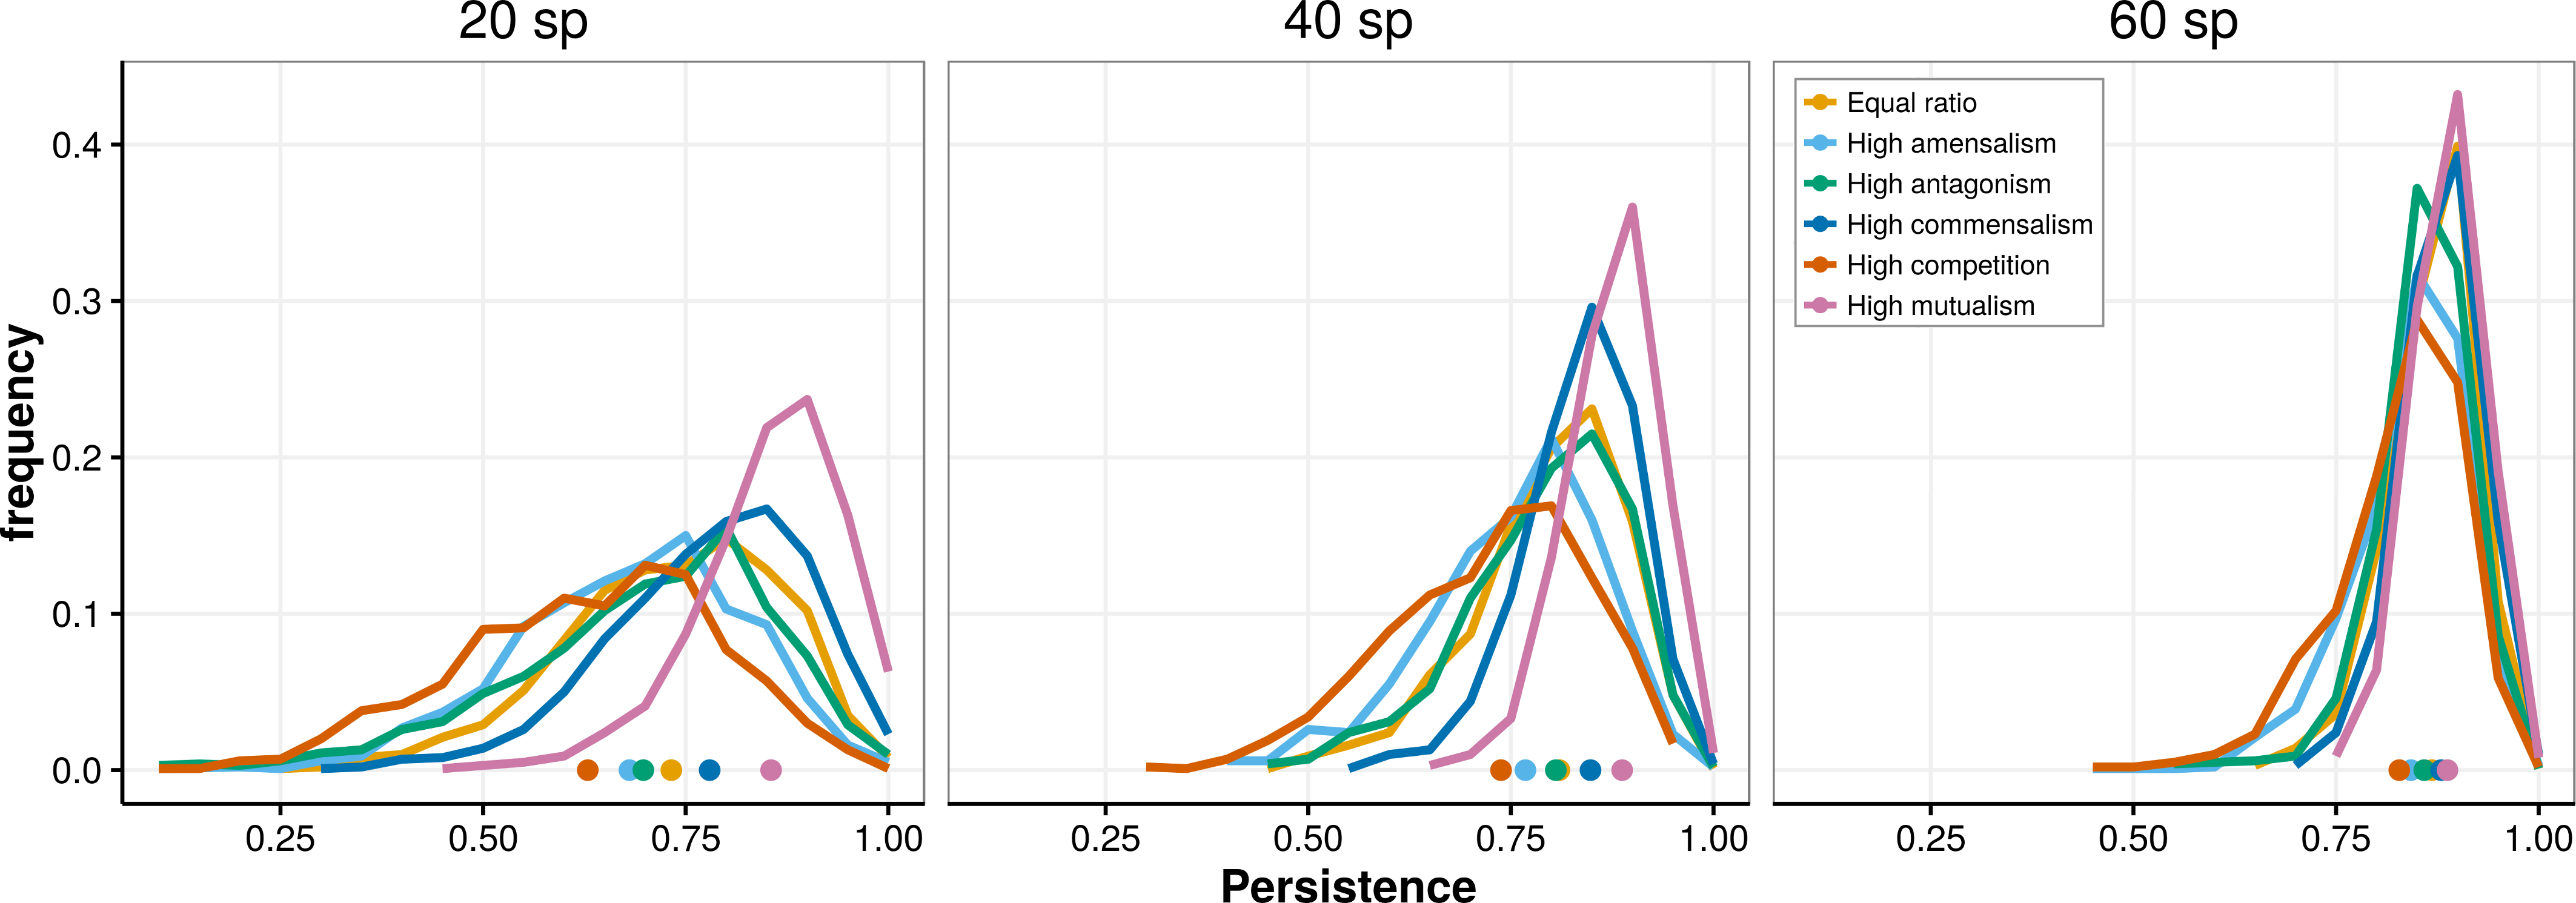
\includegraphics[width=\textwidth]{./Figures/chapter03/Fig_2.png}
\caption[Persistence of model communities]{\color{Gray} Persistence values of the simulated communities at the end of the simulations. Vertical axis represents the relative frequency of a given persistence value in the pool of replicates (1000 replicates for every combination of initial richness and initial frequency of interaction types). All resulting pairs of persistence distributions but one are significantly different according to Kruskal-Wallis rank tests (\cref{tab:tableApp3.2.1}) and post-hoc Dunn’s tests (\cref{tab:tableApp3.2.2}).}
\label{fig:fig3.2}
\end{figure}

\FloatBarrier

\subsection*{Which types of biotic interactions are more likely to be lost, as species go extinct?}

In our model, local extinctions have structural consequences for the remaining network: when a species goes extinct, its interactions disappear as well and are not replaced. The initial and final frequencies of the different interaction types were significantly different in most cases (Fig. \ref{fig:fig3.3}, results of statistical tests in \cref{tab:tableApp3.2.3}). Amensalism and competition tended to decrease in relative frequency with respect to initial levels, while mutualism tended to increase. Antagonism and commensalism responded differently for varying levels of community richness. Antagonistic interactions decreased in frequency only in communities with 20 initial species, while in communities with 60 species, they increased; the opposite was observed for commensalism, which increased in species-poor communities but decreased with high species richness.

\begin{figure}[!ht]
\centering
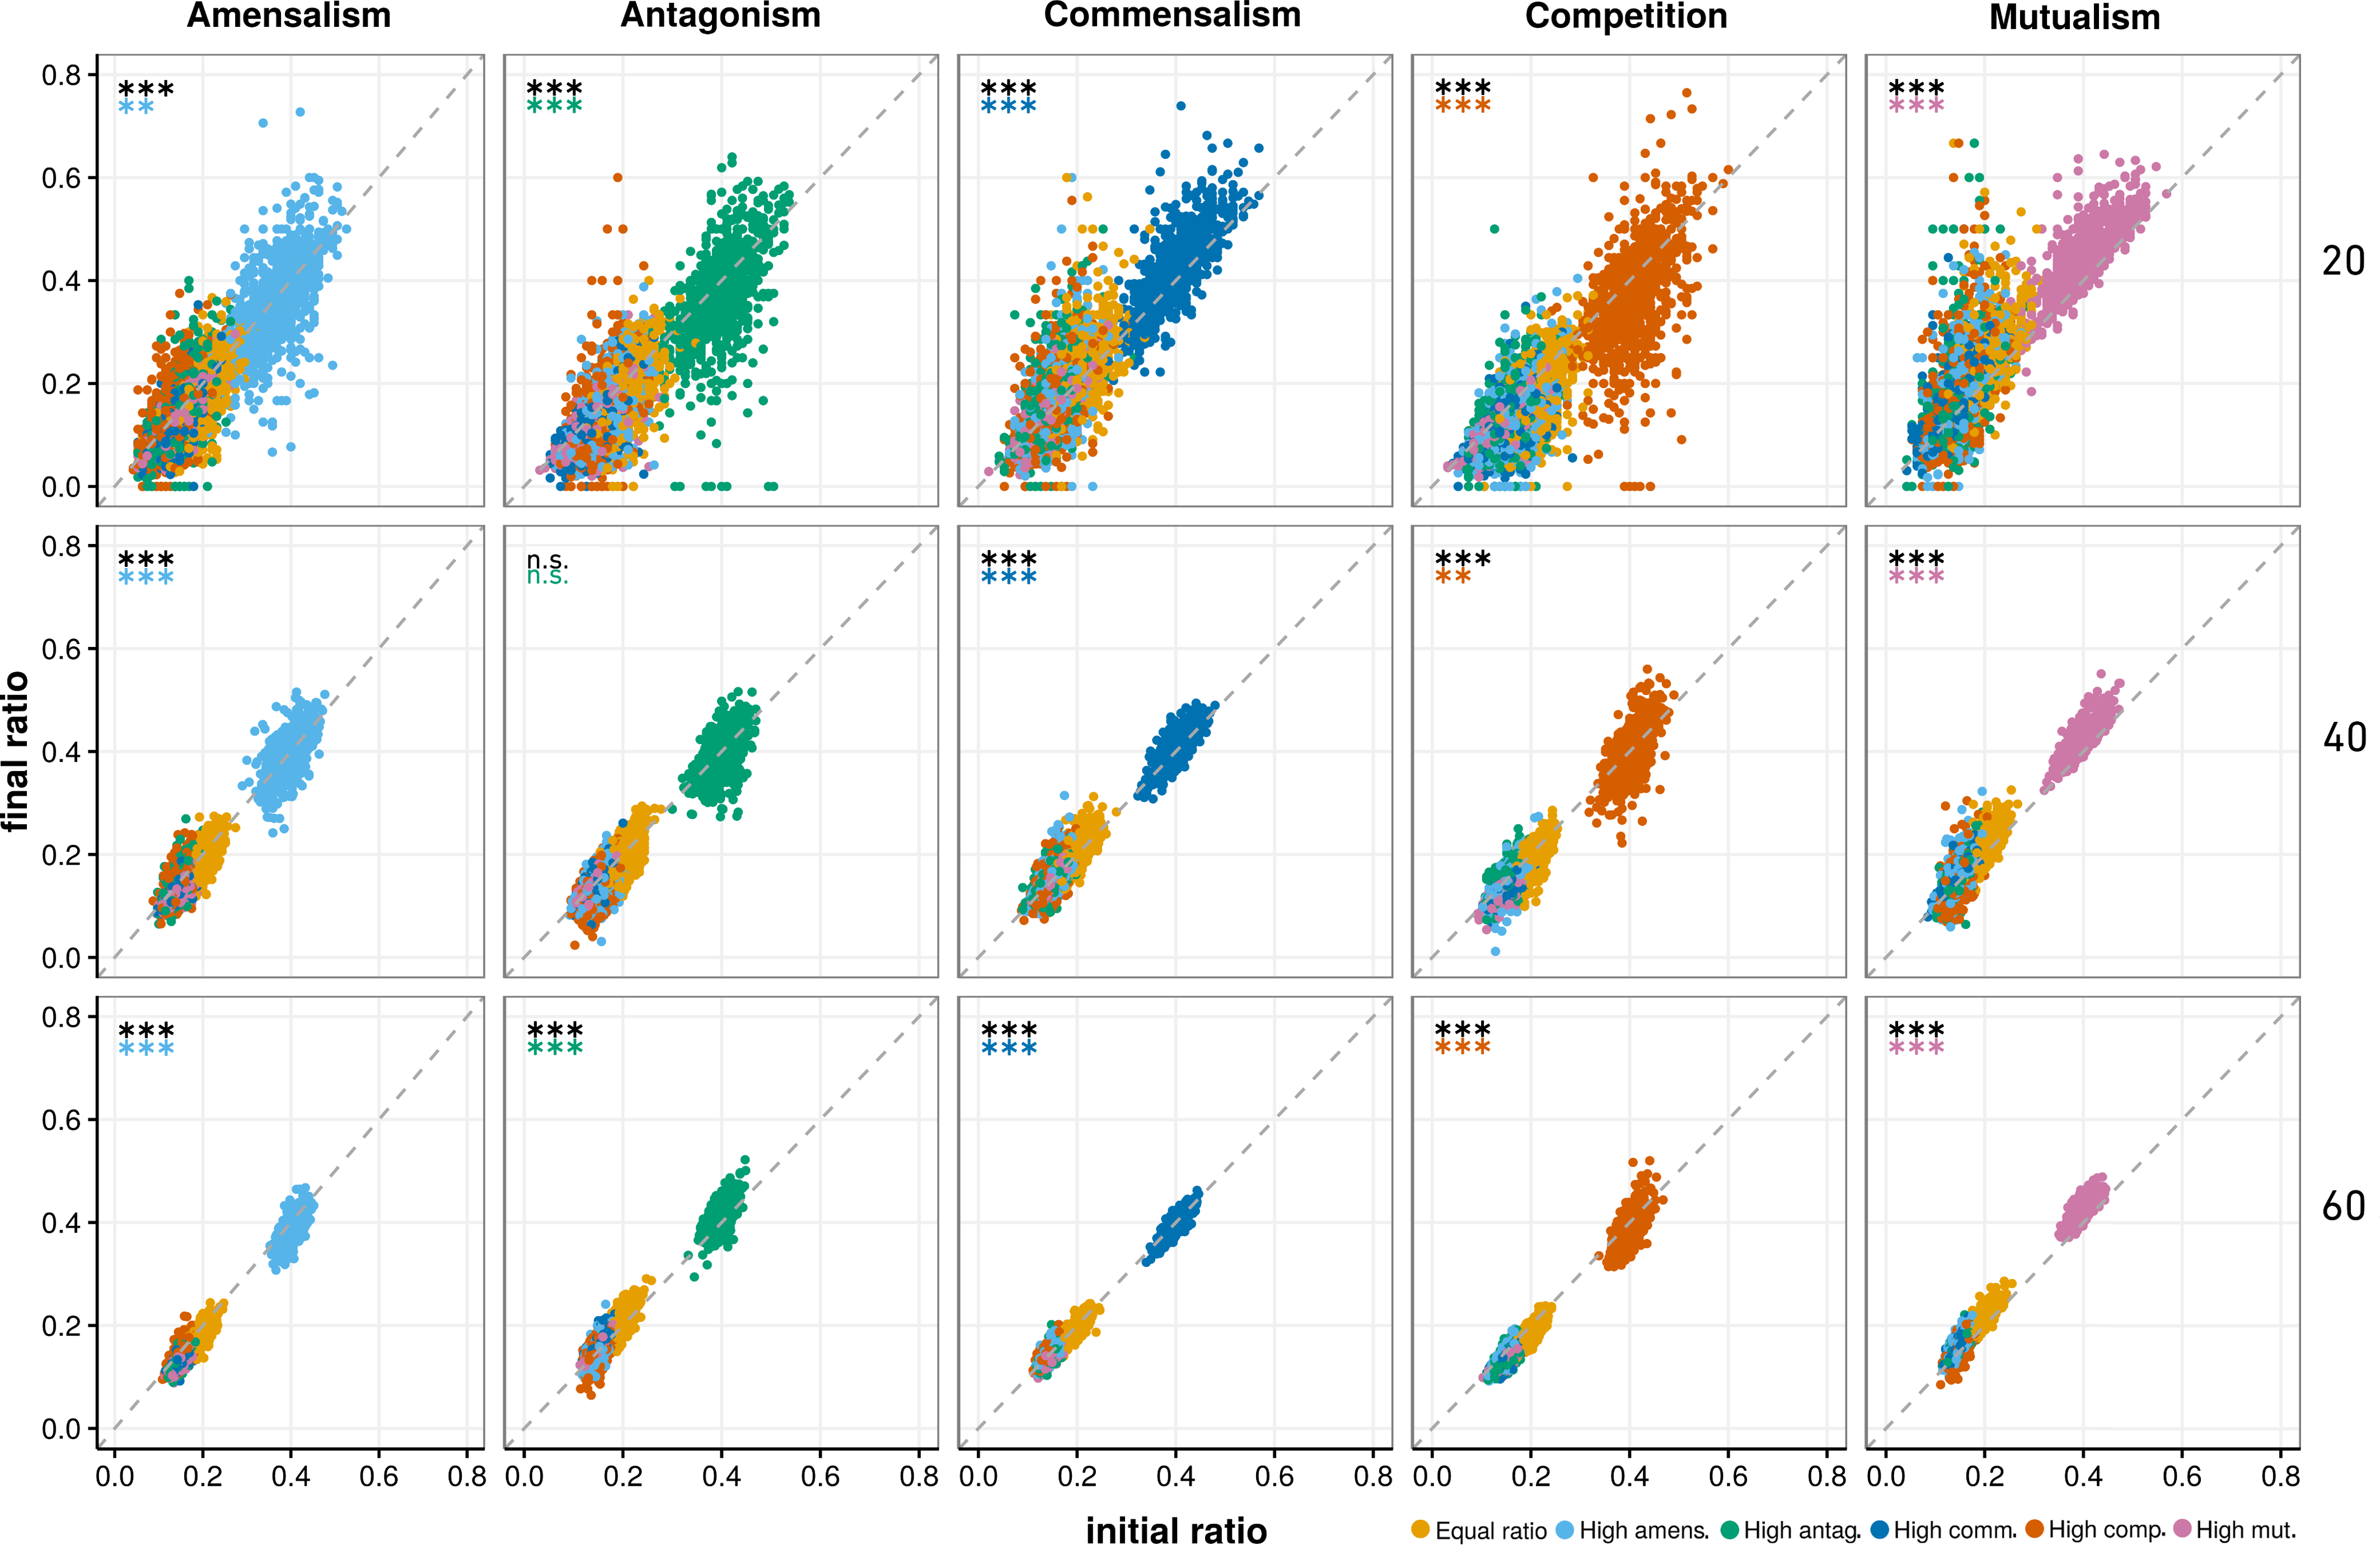
\includegraphics[width=\textwidth]{./Figures/chapter03/Fig_3.png}
\caption[Initial and final interaction ratios]{\color{Gray} Initial and final frequency of each interaction type in each community parameterization (rows: richness levels, columns: interaction frequencies levels). Each dot represents a single simulation, color code is the same as Fig. \ref{fig:fig3.2}. Upper left symbols in each panel represent the significance of the difference in initial and final ratios according to Wilcoxon signed rank paired tests, in black for the whole set of simulations, and colored for the simulations with high ratio of the respective type (n.s.: p-value > 0.05, *: p-value $<$ 0.05, **: p-value $<$ 0.01, ***: p-value $<$ 0.001. See \cref{tab:tableApp3.2.3} for details.}
\label{fig:fig3.3}
\end{figure}

\FloatBarrier

\subsection*{Does our model reflect structural patterns observed in empirical networks?}

Focusing on the structural features listed by Jacquet et al. (2016), we checked three features observed in empirical networks: the distribution of interaction strengths (species impacts in our scheme), their variation in magnitude with trophic level, and the correlation of antagonistic pairwise interaction impacts. The distribution of species impacts in our model communities ($I_{i,j}$ in Eq. \ref{eq:eq3.1}) was positively skewed in all cases, with communities with high proportion of negative interactions being the most skewed (Fig. \ref{fig:fig3.4}, \cref{tab:tableApp3.2.4}). The magnitude of species impact decreased consistently with increasing trophic level (Fig. \ref{fig:fig3.4}, \cref{tab:tableApp3.2.5} and \cref{tab:tableApp3.2.6}). Lastly, there was a significant negative correlation in the values of pairwise species impact for antagonistic interactions (Fig. \ref{fig:fig3.4}, Wilcoxon signed-rank tests, $V = 0$, $p < 0.001$ in all cases).

\begin{figure}[!ht]
\centering
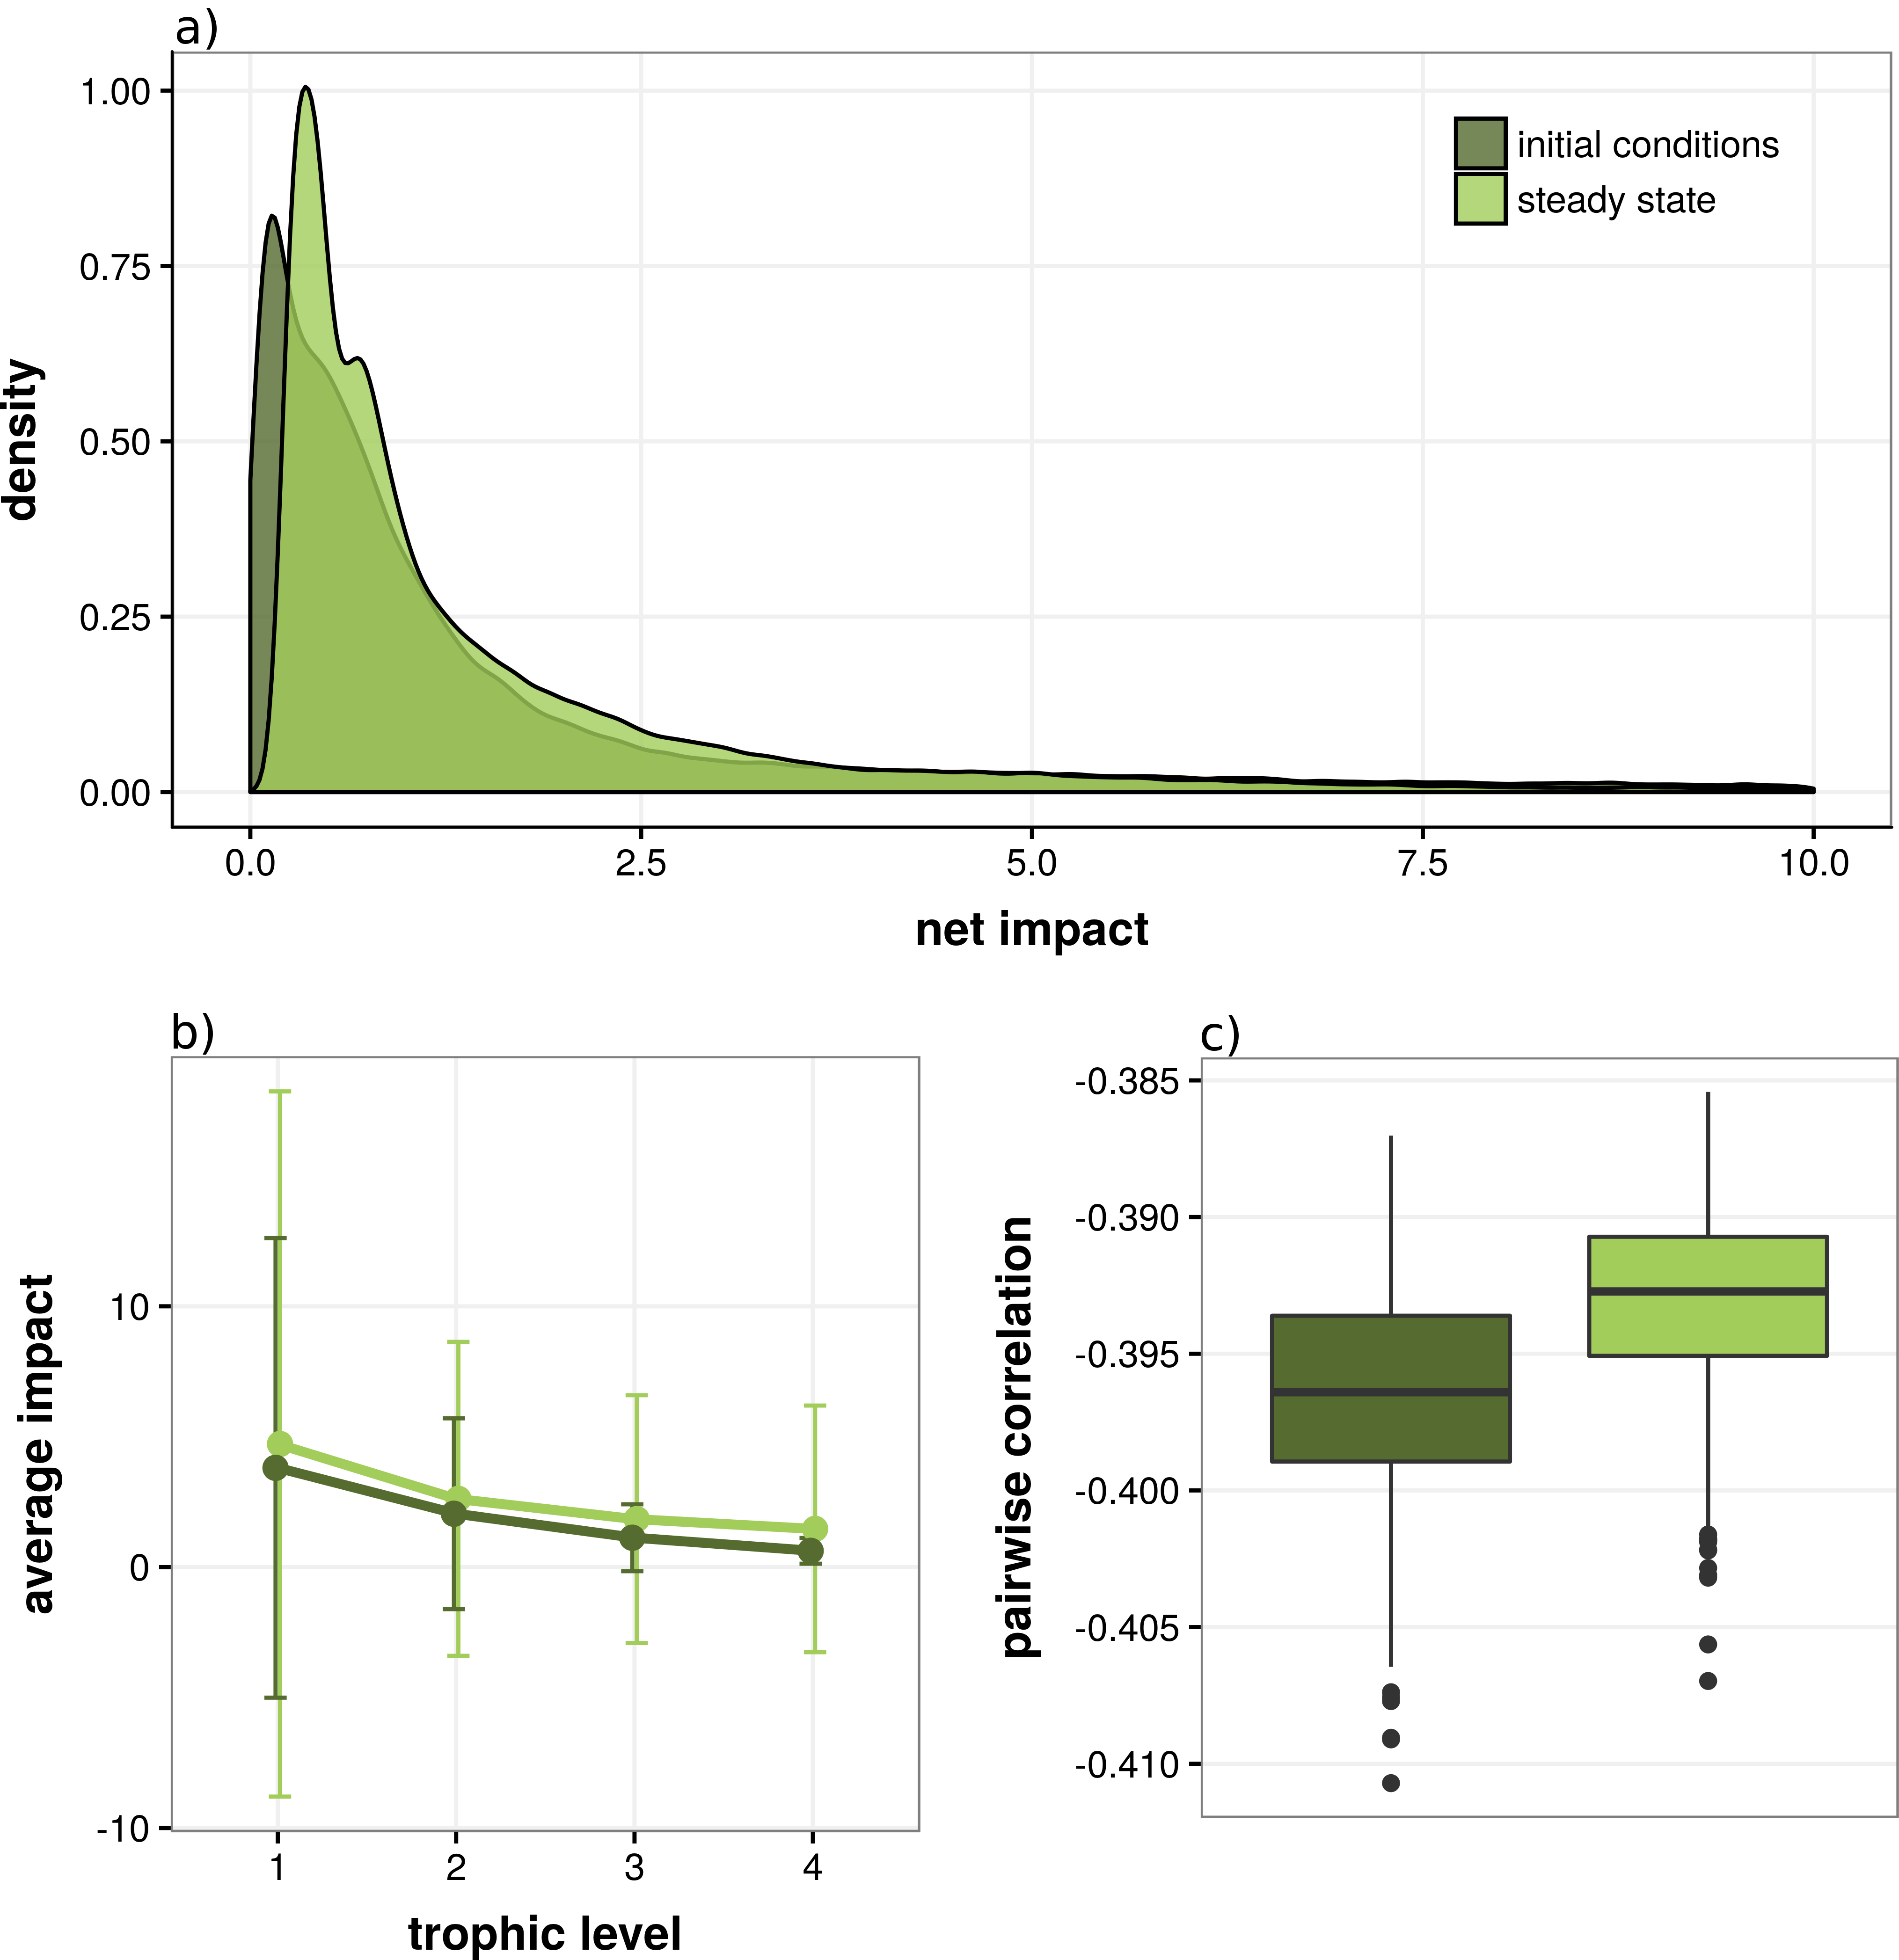
\includegraphics[width=.7\textwidth]{./Figures/chapter03/Fig_4.png}
\caption[Community structural patterns]{\color{Gray} Structural patterns observed in our model, at the initial and final steps of the simulations. Data shown corresponds to simulations with an initial richness of 60 species and equal probability of occurrence for every interaction type. a) Skewed distribution of species impacts. b) Decrease in average impact per trophic level (error bars represent an interval of one standard deviation centered in the mean). c) Correlation of species impact among pairs of species. In this panel, the only interactions accounted for are antagonistic ones.}
\label{fig:fig3.4}
\end{figure}

\section{Discussion}

Our simulations indicate, primarily, that positive interactions are key for maintaining species persistence, particularly in species-poor communities. For understanding the outcomes of our model and in order to place them in a general context, we first evaluate the role and implications of modeling interaction impacts based on species abundances and interaction frequencies. Secondly we analyze the combined influence of other community-level factors.

\subsection*{Species persistence and pairwise direct interactions}

All other things being equal, the number of interactions every species has with other species (i.e., their degree) is expected to increase with increasing number of species in the community. This is exactly what we recorded in our model communities: by keeping network connectance constant, we obtained average degrees of 9.5 for communities of 20 species, and degrees of 19.5 and 29.5 for communities of 40 and 60 species, respectively (values not far from the empirical estimates obtained by \cite{Kefi2015}, who reported an overall connectance of 0.47 for a community of 104 species, and thus a mean overall degree of 24.2). Given such a scenario, in species-poor communities the dynamics of a species will directly depend on only a handful of pairwise interactions. In such cases, a single interaction with high impact will have a disproportionate direct effect on species dynamics and, by extension, the prevalence of negative or positive interaction types will be an important driver of persistence at the community level.

The direct impact of interactions in communities is not only dependent on their numbers, but also on the abundances of the interacting species. Considering a skewed SAD (Species Abundance Distribution) of the overall community, as in our main simulations, the percentage of rare species (e.g. these with $<$ 10 individuals) increases and then stabilizes with increasing richness, while the percentage of very abundant species (e.g. with > 100 individuals) decreases (\cref{tab:tableApp3.2.7}). In species-poor communities, thus, a higher proportion of interactions will involve very abundant species, increasing the probability of comparatively strong direct impacts on species dynamics. As richness increases, more interactions will take place between comparatively rare species. The average impact per interaction will decrease accordingly (\cref{fig:figApp3.2.2}), with the effect that average persistence will increase regardless of the distribution of interaction types.

An important consequence of the differential effect of interaction types on species persistence is that species engaging in a high number of direct positive interactions will tend to persist and maintain their interactions, whereas species with a high number of direct negative interactions will tend to go extinct more frequently and, thus, their associated interactions will be lost, increasing the overall ratio of positive interactions (Fig. \ref{fig:fig3.3}). This reasoning is, however, contingent on the modeling assumption that there is no interaction rewiring. Keeping in mind this strong assumption, if these results hold, natural assemblages should be filtered to maintain a relatively high ratio of direct positive interactions, in particular in species-poor communities, and species with a high degree of negative interactions will be rare and, in any case, have otherwise strong life-history traits that allow them to persist. Note that, throughout the study, we limit our discussion to the role of direct interactions. The importance of indirect or net effects for understanding community patterns is well established (e.g. \citealt{Montoya2009a}), and the mechanisms proposed here for linking species interactions, abundance and persistence, would be improved by accounting for the role of these higher-order effects. However, in model networks, net effects are commonly analyzed by calculating the negative of the inverse Jacobian matrix \citep{Novak2016}. The formulation of our model, without static interaction coefficients and, potentially without attaining static equilibria, limits the applicability of analyses based on Jacobian matrices. Therefore, we opted not for calculating net effects and leave their analyses in our framework for future studies.

By explicitly modeling species impacts based on species abundances and interaction frequencies, our interpretation of species persistence and community dynamics differs fundamentally from that of other theoretical models of multiple interactions (e.g. \citealt{Mougi2012}). Furthermore, our response factor, species persistence, also differs from the common local stability analyses performed in the majority of theoretical network studies. Despite these fundamental differences, some common trends seem to surface. Much like our finding that the frequency of interaction types is less important in speciose communities, in the study by \cite{Mougi2012} increasing richness allowed for high local stability regardless of the proportion of positive to negative interactions (but see \citealt{Suweis2014}). With a completely different methodology, built on individual-based models, \cite{Lurgi2016} further found that increasing the proportion of mutualistic links increased overall stability in their model. Yet another, more general interaction model showed that positive interactions tend to become dominant in interaction networks as a consequence of spontaneous self-organization \citep{Jain2001}. Overall, these independent lines of evidence point to the combined importance of positive interactions and community size on stability patterns in a broad sense.

The relationship between species richness, abundances and interaction types may shed light on other general questions in community ecology, aside from the comparison with previous theoretical models.

First, in line with empirical findings from plant communities in stressful environments \citep{Soliveres2014, Cavieres2009}, we have shown that a high ratio of positive to negative interactions significantly increases species persistence, particularly in communities with low initial richness. By the explicit consideration of four discrete trophic levels, we show that a preponderance of positive interactions is particularly important for the persistence of intermediate consumers (\cref{fig:figApp3.2.1}), upper panels). These species are preyed upon by top predators and also subject to competition (both direct as modeled and indirect as a result of resource consumption) and amensalism. Hence, they are potentially the most benefited from engaging in mutualisms with species from adjacent trophic levels. As mutualistic interactions are most prevalent across adjacent trophic levels (Fig. \ref{fig:fig3.1}), intermediate species will be the ones showing a highest degree of these positive interactions. Note that we did not model competition for resources at the basal trophic level, and all our communities included a fourth trophic level of top predators. Thus, these latter species, not subject to predation (aside from a very small probability of intraguild predation, Fig. \ref{fig:fig3.1}), are likely to have a strong top-down influence on the persistence of intermediate species.

Second, our findings contribute to reframing the debate on whether pairwise interactions are stronger in richer communities. On the one hand, the hypothesis of a gradient on pairwise interaction strength with latitude has been generally supported on empirical grounds (\citealt{Schemske2009}, but see \citealt{Moles2016}), but it is unclear whether or how this pattern is affected by the richness of the analyzed communities. On the other hand, we have shown that if interaction impacts are neutral (i.e. driven solely by species abundances), then species impact will generally decrease with increasing richness. This theoretical result has been partially supported in a recent study that found that, on islands whose size granted a certain environmental stability, the strength of competitive and antagonistic interactions decreased with island size and richness \citep{Schoener2016}. Clearly, an array of factors can cause deviations from neutrality in interaction strengths (IS function in eq. \ref{eq:eq3.1}), and hence the neutral interactions hypothesis should be viewed as a baseline for estimating species impacts when no other information is available. Such neutral estimations have already been applied for plant-pollinator networks \citep{Vazquez2012} or in sampling campaigns of multiple interactions networks \citep{Pocock2012}.

\subsection*{Emerging community structure further enhances persistence}

Components of community structure, such as species diversity or different network-level metrics, have been regarded as key factors in previous modeling studies \citep{Sauve2014,Sauve2016}, where accounting for empirically informed values generally enhances stability metrics. Such theoretical results are, however, difficult to validate, since empirical data on communities with varying structural patterns is extremely scarce. As an alternative for testing the adequacy of our model, we analyzed whether our model communities displayed properties comparable to those found in empirical networks. Recently, \cite{Jacquet2016} showed that empirical food webs possess three structural characteristics that clearly differentiate them from random counterparts: first, they display the classic skewed distribution of interaction strengths, whereby there are very few strong interactions and a majority of weak ones \citep{McCann1998}. Secondly, empirical food webs show strong pairwise correlations in interaction strengths, in line with theoretical findings \citep{Tang2014}. Thirdly, interaction strengths are not evenly distributed across trophic levels; rather, average interaction strength tends to decrease with trophic level. In our model, the skewed distribution of species impacts and their “pyramidal” arrangement are observed and maintained throughout the community dynamics (Fig. \ref{fig:fig3.4}, panels A and B). On the other hand, the pairwise correlations generated in our model communities (Fig. \ref{fig:fig3.4}, panel C) are significantly different from zero but smaller than those reported by \cite{Tang2014}. Such disparity may be due to the lack of trait-matching mechanisms in our model, as trait-matching may give rise to increasingly specialized and correlated pairwise interactions \citep{Santamaria2007}.

The three patterns outlined by \cite{Jacquet2016}, i.e. skewed distribution of impacts, pairwise correlations in interaction strength, and decrease of species impacts with increasing trophic level, are already present at the beginning of the simulations (Fig. \ref{fig:fig3.4}), so they arise from the structural constraints of our community assembly process. It is therefore informative to analyze the dynamics of the model without these constraints, namely 1) a skewed Species Abundance Distribution of the overall community, 2) a sublinear scaling of overall abundances with increasing trophic level, and 3) a non-random distribution of links across trophic levels, for each interaction type (Fig. \ref{fig:fig3.1}).

Relaxing these constraints does not modify the main qualitative patterns of our results, i.e. positive interactions and, to a lesser extent, increasing richness, have a positive effect on persistence (\cref{fig:figApp3.3.1}), but quantitative outcomes vary. The effect of removing the second and third constraints on species persistence is negative, while removing the first constraint has a generally positive effect on persistence. This effect is particularly strong for upper trophic levels, where average persistence varies widely depending on the assembly constraints imposed (\cref{fig:figApp3.3.2}). These results invite the interpretation that community structure, both in terms of the topology of the different interaction types and the distribution of species abundances across trophic levels, is a key factor for maintaining high levels of persistence. Despite their recorded importance, understanding of these factors in empirical communities is still limited. Further empirical work is needed to evaluate the generality of the abundance scaling law \citep{Hatton2015} for multiple trophic levels and community types, and, importantly, to understand its underlying mechanisms. Regarding the distribution of interaction types, our approach was to assign probabilities of occurrence based in empirical observations. This methodology is biased towards the most studied interaction types (antagonism, competition and mutualism), and towards easily observed organisms and interactions, thereby failing to account for functionally important yet rarely considered organisms, such as microorganisms, parasites or parasitoids. It has been shown, for example, that accounting for parasites when analyzing food webs significantly modifies network structural patterns \citep{Lafferty2006}, so the interaction probabilities obtained here should be taken as broad estimates. Despite these shortcomings, evidence is increasing theoretically and empirically that link topology is key not only for consumer-resource, but for all interaction types \citep{Pocock2012,Evans2013a,Kefi2015,Kefi2016a,Sauve2016}. Due to the difficulty in obtaining reliable estimates of multiple interactions at once in empirical communities \citep{Garcia-Callejas2018}, we currently do not know whether the distribution and topology of interaction types is homogeneous across communities or how it is influenced by habitat type or environmental factors.

The significant variation in persistence ratios with structural patterns shown here suggests that theoretical studies relying on idealized communities (e.g. totally mixed interactions and/or random distributions of biomass across trophic guilds) are likely to miss key mechanisms for maintaining species persistence. Rather, future studies on multiple interactions networks should take into account the variability of community-level factors present in natural assemblages, like interaction frequencies and distribution, or abundance scalings across trophic levels. Our model is a first step in that direction, but it is important to note that the insights obtained are, of course, contingent on the assumptions made. In particular, important features of the model are the constant connectance hypothesis and the implementation of dynamic interaction impacts. Furthermore, we assumed that the degree of a species is independent of its relative abundance in the community. While none of these assumptions hold completely true in nature, they represent convenient starting hypotheses for modeling complex ecological communities, because ecological interpretations can be drawn when empirical systems deviate from these assumptions \citep{Banasek-Richter2009}. Further investigation on the differential functional form of the different interaction types, e.g. as outlined for mutualism by \cite{Holland2002}, and on interaction rewiring \citep{Valdovinos2010,Mougi2016b}, will also help refine the conclusions obtained here. Aside from these potential developments, our results can be used to establish baseline predictions on the dynamics of natural communities across gradients of richness or other factors. In that regard, the sensitivity of species-poor communities to interaction diversity is of particular interest: as these communities are particularly endangered by anthropogenic drivers of ecosystem change \citep{Cavieres2009}, it is paramount to evaluate this theoretical result and its potential consequences for management and conservation schemes.

\section{Conclusions}

To understand how the persistence of species is influenced by the complex networks of interactions in which they are inserted, it is important to develop models that account for the diversity of interactions present in nature, and that incorporate realistic constraints to the structure of these networks. By developing one of such models, we found that species' local persistence is not explained by a single axis of variation in network properties, but rather is contingent on the interaction of several structural factors: the diversity and distribution of biotic interactions, the size of the community, and the distribution of species abundances across trophic levels. In particular, we found that a high prevalence of positive interactions can lead to increased persistence of species in communities with low richness, whereas speciose communities can sustain varying ratios of interaction types without significant decreases in average persistence. Although simulation studies are, by definition, affected by a number of simplifying assumptions, we found that our simulated networks have emerging features also present in empirical networks, suggesting that our modeling framework captures part of the mechanisms that maintain the richness and diversity of natural assemblages. The insights from network models, such as ours, are one of the complementary ways in which ecologists approach the understanding of local species persistence, and should prove valuable in developing a robust predictive framework for its variation across different types of gradients.

%%************************************************
\chapter[Species Abundance Distributions and trophic structure]{On the variability of Species Abundance Distributions with trophic guild and community structure}\label{ch:SAD}
%************************************************

\tikz[remember picture,overlay] \node[opacity=0.3,inner sep=0pt] at (current page.center){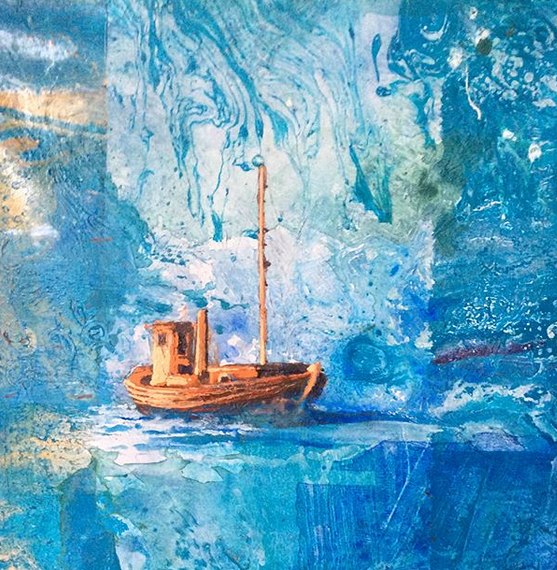
\includegraphics[width=\paperwidth,height=\paperheight]{./Figures/cover/barco_oceano.png}};
\clearpage

\section*{Abstract}

Species Abundance Distributions (SADs) are one of the strongest generalizations in community ecology, but their variation across trophic levels remains largely unexplored. I study the variation in SAD metrics across trophic guilds, using a theoretical model and a compilation of empirical datasets. First, I develop a model that allows tracking the variations in abundances across trophic guilds, controlling for species richness and network connectance. The theoretical results show that evenness is highest for herbivores, and decreases in omnivore and carnivore guilds. The richness and connectance of the community network are also negatively correlated with guild evenness. Second, I compare the empirical SADs of 226 terrestrial plant communities and 497 mammal communities comprising species grouped in three general trophic guilds (herbivores, omnivores, and carnivores). Sampled plant communities are significantly less even and more skewed than mammal ones. There are no significant differences in SAD metrics between the different mammal guilds, but carnivores are comparatively rare (i.e. have a higher proportion of species than individuals), whereas omnivores are comparatively more common. Species richness has a positive effect on both evenness and skewness, and spatial and temporal extent have negative effects on evenness and do not affect skewness. I argue that the difference between plant and mammal guilds can be related to higher niche availability in animals than in plants, that decreases the importance of competitive exclusion in mammal guilds. As no systematic differences were found between the SADs of mammal herbivores, omnivores, and carnivores, this may indicate similar niche availability, when averaged across habitat types, for the different animal trophic guilds.

\section{Introduction}

Most species, in any ecological community, are comparatively rare, and only a few of them are very abundant. This empirical observation is one of the few true universal laws in ecology, a pattern that is observed in all kinds of communities and guilds, from small arthropods \citep{Basset1991} to tropical trees \citep{He1997}. The Species Abundance Distribution (SAD) describes precisely this variation in species abundances within a given assemblage.

The information contained in SADs, aside from its theoretical interest in understanding community dynamics \citep{Hillebrand2008}, can be of interest for conservation and management \citep{Matthews2015} or for estimating ecosystem functions such as primary productivity \citep{Wilsey2000}. It is therefore important to understand which are the main axes of variability in SAD shape across guilds, and what are the ecological processes underlying this variability. So far, important efforts have been devoted to understand variation in species abundances across enviromental gradients \citep{Ulrich2016, Passy2016}, levels of disturbance \citep{Komonen2017}, spatiotemporal scales \citep{Borda-de-Agua2012}, or multiple factors combined \citep{Arellano2017}. Intrinsic differences in species-level traits among the species that make up the community will also be reflected in the SAD. For example, core and satellite species of an ecosystem are likely to differ in their intrinsic abundances regardless of other factors \citep{Magurran2003}, and the degree of trophic or habitat specialization of different species may also be related to their relative abundances \citep{Labra2005, Matthews2015}.

Despite these significant advances, in the debates on the mechanisms that shape SADs, virtually all theories and hypothesis that relate SAD shape to ecological processes at the local scale refer to horizontal communities, i.e. communities of a single trophic level. Thus, these theories emphasize the role of either neutral dispersal and drift \citep{Hubbell2001} or horizontal selection \citep{Vellend2016}. But natural communities form a complex network of species linked by different types of biotic interactions both horizontally (within a given trophic guild) and vertically (across trophic guilds, Fig. \ref{fig:fig4.1}). The influence of the interaction topology on the abundance patterns of the different guilds of a community has, to my knowledge, never been explored systematically.

\begin{figure}[ht!]
\centering
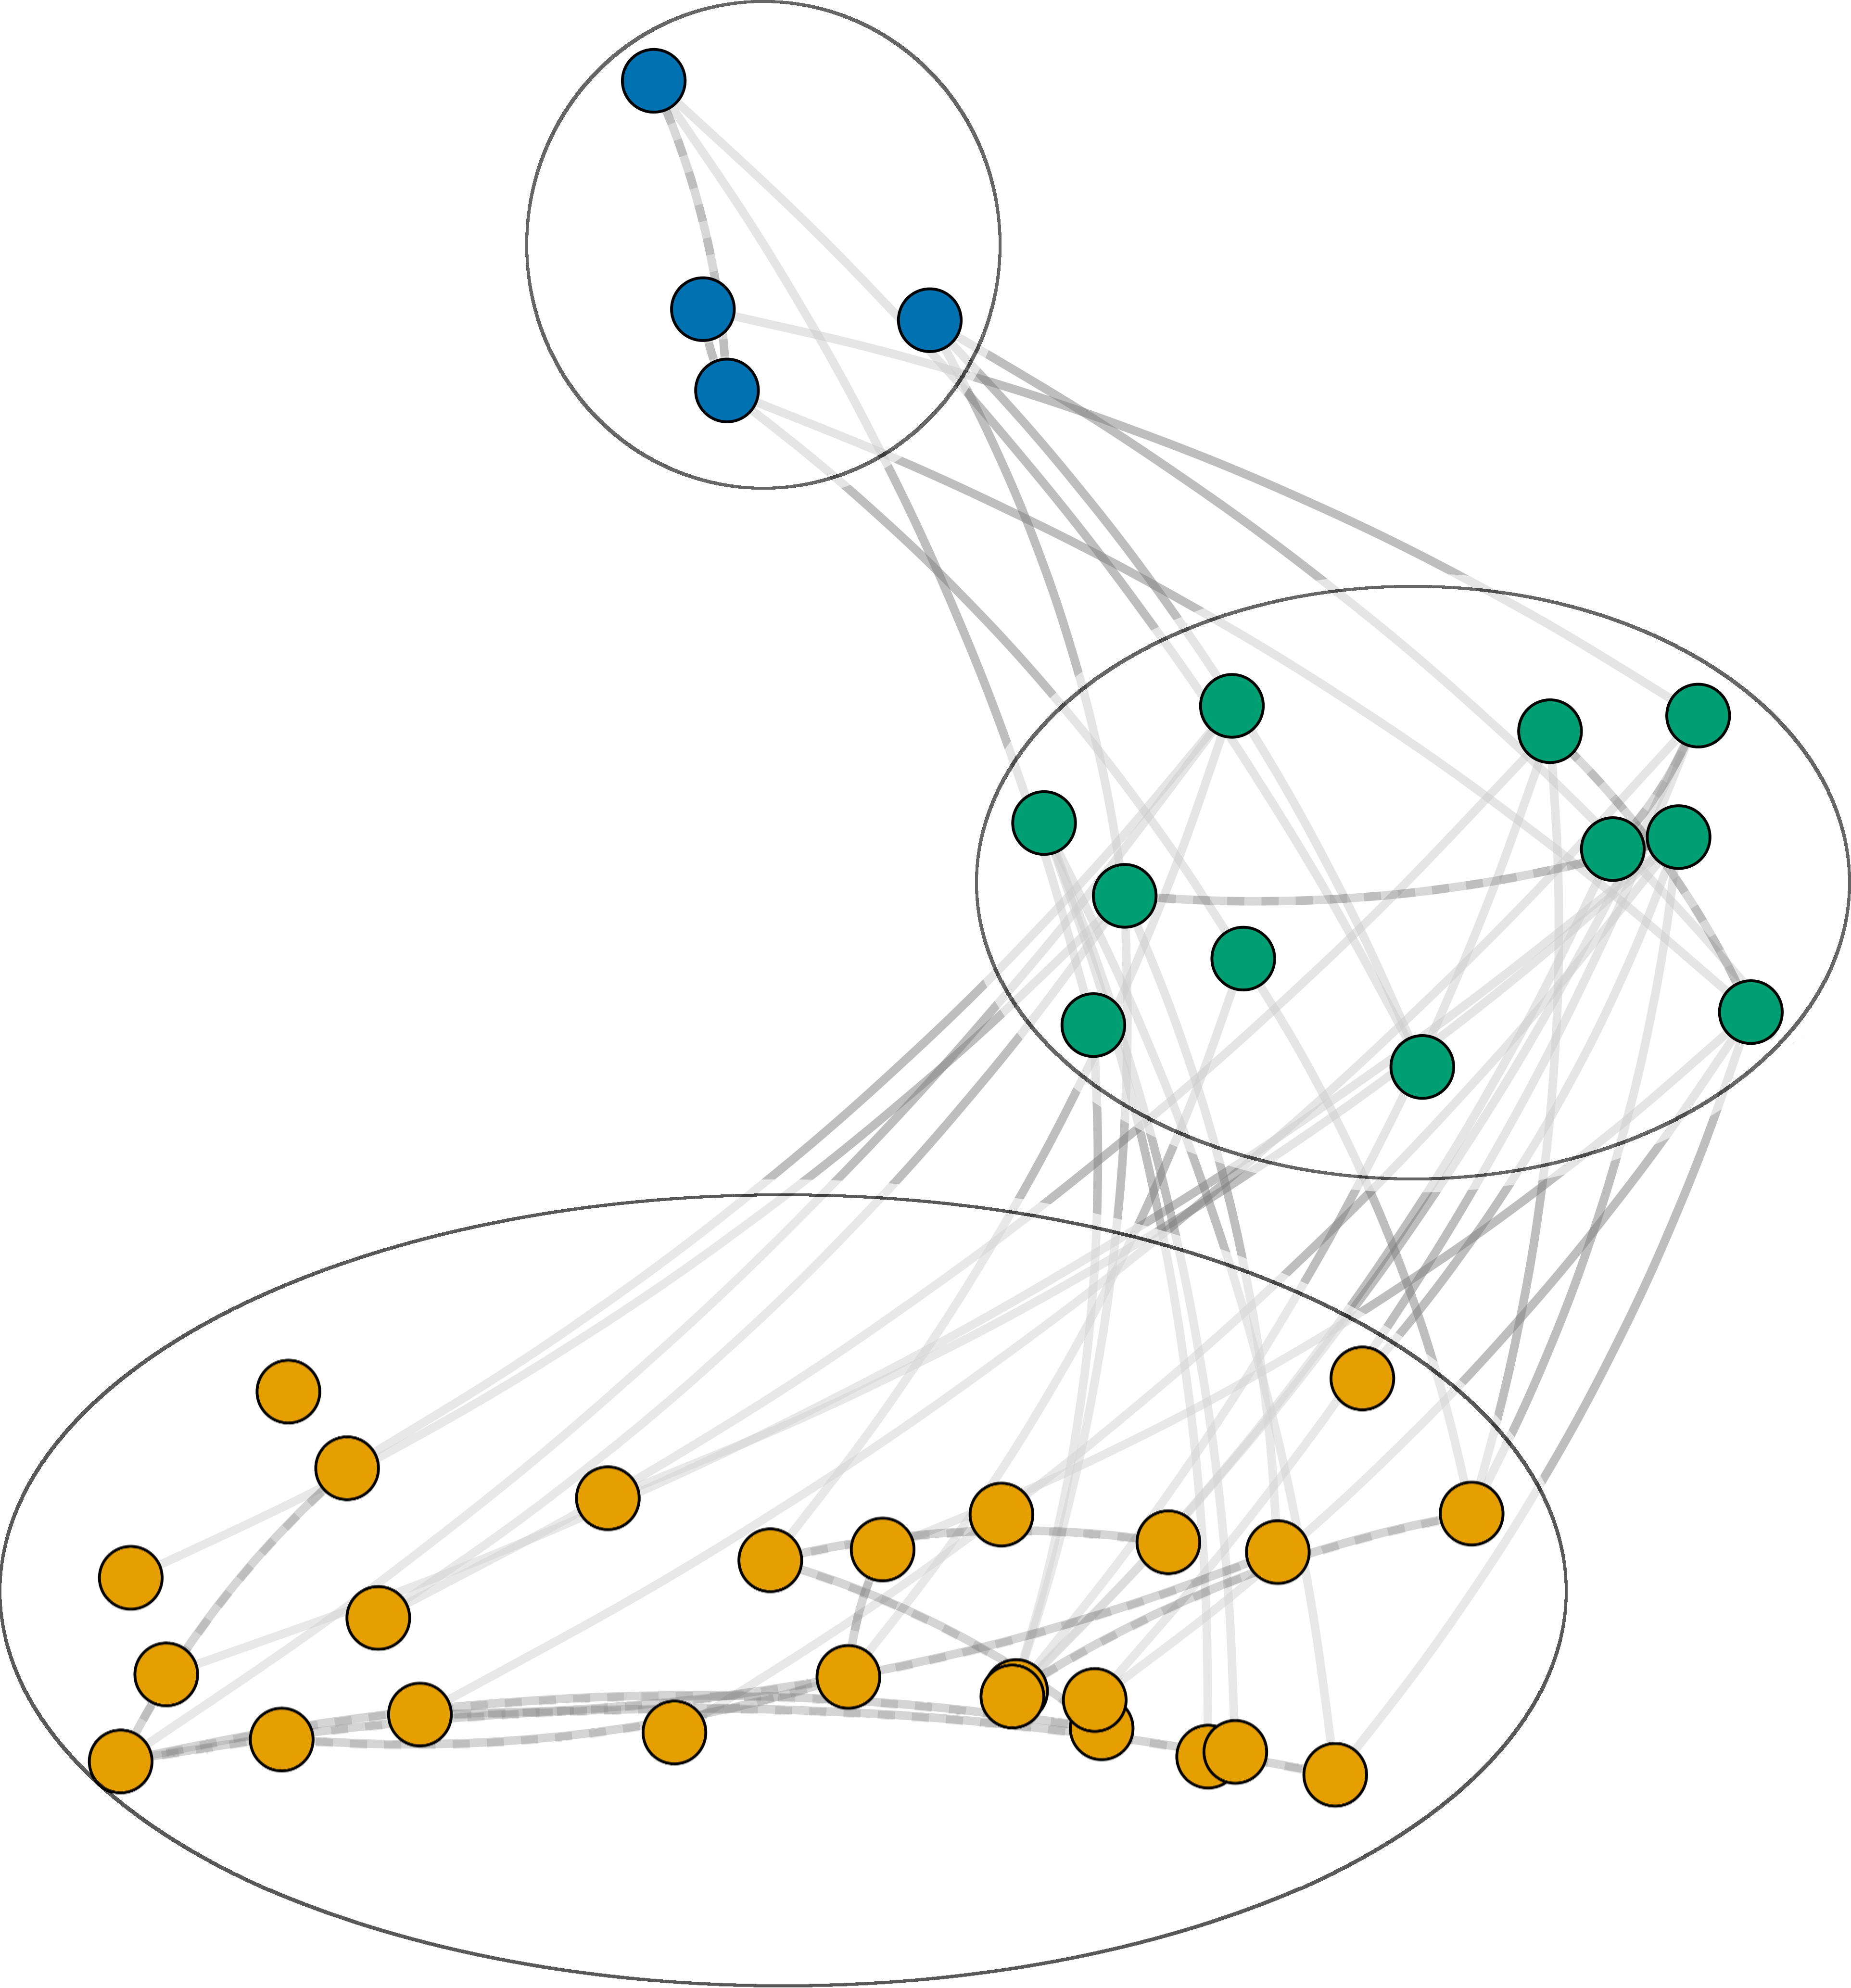
\includegraphics[width=0.5\textwidth,height=\textheight,keepaspectratio]{./Figures/chapter04/Fig_1.png}
\caption[Schematic multi-trophic community]{\color{Gray}A schematic ecological community with three disjoint trophic guilds. The areas within the ellipses represent the domain of horizontal community ecology that is the subject of most SAD studies, focusing on intra-guild interactions (dashed grey lines) and assuming that interactions with other guilds (full grey lines) are negligible. In this study, I focus on how interactions across guilds drive variations in SAD metrics.}\label{fig:fig4.1}
\end{figure}

In complex, multitrophic ecological communities, trophic guilds (sensu \citealt{Fauth1996}) differ in fundamental properties that can potentially be reflected in their associated abundace distributions. First, several studies have demonstrated that basic descriptors, such as biomass or species richness, vary predictably with trophic level (e.g. \citealt{Lindeman1942,Odum1957,Turney2016}). Focusing on the relationship between two adjacent trophic levels, \cite{Hatton2015} showed that the biomass of empirical guilds of herbivores and their associated predators scales generally with a power-law of exponent 3/4. They also showed that, in their data, the relationship between mean body mass and community biomass is non-significant for most of the functional groups they studied. As such, if body mass varies in a similar fashion in different trophic levels, the scaling in biomass should also be reflected in a scaling on number of individuals at each trophic level, as foretold by Ramón \cite{Margalef1980}.

Other patterns associated to the distribution of abundances, such as species rarity or the degree of dominance, can potentially vary across different trophic guilds, but empirical evidence is scarce. In a study of macroinvertebrate communities, predators showed a higher proportion of species than of individuals in the overall community \citep{Spencer2000}, pointing to a higher rarity in predator species. Furthermore, \cite{Spencer2000} showed that predator and non-predator species did not vary significantly in the ratios of dominance of the most abundant species. More recently, \cite{Dornelas2011} showed that relative dominance decreased consistently with increasing richness in communities of freshwater fish.

Overall, these lines of evidence suggest a complex, combined influence of the richness and trophic position of a guild on its abundance patterns. In a first approximation, the number of different resources available to a given trophic guild and the partition of these resources among its constituent species \citep{Tokeshi1990, Sugihara2003} will ultimately drive the guild's SAD. As the trophic interactions among guilds are encoded in the topological structure of the community food web, this structure is likely to play a role in modulating SAD variability across guilds.

Analyzing abundance distributions in communities comprising several trophic guilds is complicated further by a number of factors. For example, movement capacity generally increases with trophic position \citep{McCann2005}, and in turn, it significantly influences SADs and their variation with sampled area \citep{Borda-de-Agua2017}. Therefore, different trophic guilds in the same community will likely require varying sampling areas in order to obtain their abundance patterns in a consistent fashion (see also \citealt{Holt1999}). Another issue that needs to be considered when comparing trophic guilds of different communities is precisely how to divide species among guilds in a general way. Broad categories such as herbivores/omnivores/carnivores provide groupings applicable to communities of different ecosystem types, but are likely to be too general, lumping together species with very different ecologies. On the other hand, clearly defined guilds for a given community type (e.g. sap-feeding insects in salt marsh grasses) will be too specific to allow comparisons with guilds from other ecosystem types. Therefore, a robust analysis of the role of trophic guild in SAD metrics needs to control for (1) the variations in richness across guilds, (2) the spatial and temporal extent of the data collection, and (3) the process of defining trophic guilds in a general and informative way.

Here I approach the general question of whether SAD metrics vary predictably across trophic guilds, in two complementary ways. First, I combine a model of food web structure with niche apportionment schemes for studying how SADs of different trophic guilds vary in model communities with varying network structures. Second, I analyze SAD patterns of two well-resolved datasets on community abundances of plants \citep{Phillips2002} and mammals \citep{Thibault2011}. I compare SAD patterns of plant communities and three mammal trophic guilds, controlling for guild richness, spatial and temporal extent of the data collection.

\section*{Methods}

\subsection*{The relationship between SAD properties and trophic guild: A theoretical model}

Analyses of species abundance distributions are based, on their first stage, on the grouping of species that are supposed to share certain properties of interest, such as taxonomic relatedness, spatial location or resource use \citep{Fauth1996}. As a starting point, I focus on the role of the different trophic guilds in a local multi-trophic community. Intuitively, the variability in number of individuals between species of a given trophic guild will depend on inter-specific variation in both species-level traits and resource use. Assuming, as a working hypothesis, that the main difference between species within a guild is in their competitive ability to acquire resources, it can be hypothesized that the degree of resource overlap between the species will play an important role in determining their variations in abundance \citep{Sugihara2003}. Consider a single herbivore species that is preyed upon by a number of predators. All else being equal, the partition of the prey resource will be driven by the competitive ability of these predators, and will be reflected in their own abundances (an energetic view of abundance, \citealt{Isaac2013}). When an arbitrary number of prey species can be exploited by the predators, the specialization level of the predators will influence the degree of exploitative competition between them, and indirectly its distribution of abundances. In network terminology, the level of specialization of a species is given by its degree, the number of interactions in which it engages, and indirectly, by the connectance of the network, the ratio of realized to potential interactions in it.

This qualitative hypothesis can be more precisely formulated by combining models of network structure and resource partitioning schemes. In particular, I generated food webs with varying connectance and richness values. Then, I grouped their constituent species in trophic guilds, calculated the expected abundances of each species according to a resource apportionment model, and compared the resulting distribution of abundances of the different guilds. There is a long tradition of resource partitioning models along a single axis, and here I implemented the Random Fraction model, which has been shown to fit empirical datasets reasonably well \citep{Tokeshi1990}. In this scheme, the resource is divided sequentially into fractions, until each consumer is given a fraction of the available resource. At each step, the fraction that is divided is randomly chosen, so that either the biggest fraction could be divided, leading to more equitable distributions, or the smallest fraction, leading to a bigger share for a single species. This scheme generates dominance hierarchies intermediate between a purely \textit{dominance preemption} scheme, in which dominant species always gets the higher share of the resource, and a \textit{dominance decay} scheme, in which resources are distributed most equitably \citep{Tokeshi1990}.

Food webs were generated using a modified version of the niche model \citep{Williams2000}. The original niche model takes a single niche axis in which all species are placed to generate trophic links allowing for a certain degree of intraguild predation (the original formulation is given in \citealt{Williams2000}, and its particularities with respect to other food web models are explored, for example, in \citealt{Dunne2006}). The network topologies generated with it are similar in terms of goodness-of-fit to those from more complex models \citep{Williams2008}, so it remains an appropriate model for generating food web structures in the absence of detailed information on trait structure \citep{Gravel2016}. One of its limitations, however, is the systematic underestimation of the proportion of primary producers and herbivores compared to empirical food webs. In this study, I imposed a minimum fraction of 0.2 of primary producers in the generated food webs. Furthermore, I removed all directed cycles from the web, in order to make the propagation of biomass across species feasible. For each cycle (i.e. a series of nodes and links that eventually form a closed chain), I selected one of its constituent links randomly and assigned the resource to be a basal species. These two modifications to the original model are likely to modify some emergent properties of the network structure, but the resulting connectance of the generated food webs is maintained, and the proportion of primary producers and herbivores is increased with respect to the original formulation. I grouped the species in primary producers, herbivores (i.e. species whose only feeding sources are primary producers), omnivores (species that feed in both primary producers and other species), and carnivores (species that do not feed on primary producers).

In order to obtain the abundances of the species in the food web, the abundances of the basal species need to be specified beforehand, as this model represents a static bottom-up approach. I generated basal abundances from a Weibull distribution with scale = 4.7 and shape = (0.15,0.2), derived as the average best fit from the 226 sites of the GENTRY dataset (see \textit{datasets} section).

I considered three levels of species richness (50, 100, and 200 species), and three levels of network connectance (0.1, 0.2, and 0.3). For each combination of richness and connectance, I generated 1000 networks and quantified the evenness and skewness of the SAD of the different trophic guilds (see next section).

I analyzed the variability of SAD metrics with connectance, species richness and trophic guild by using regression models. In particular, I used linear mixed-effect models (R package ``lme4'', \citealt{Bates2015}) with richness, connectance, and trophic guild as fixed effects, and replicate (e.g. the 1000 simulated networks for each combination of richness and connectance) as a random effect. As I am not interested in predictions from this model, but rather in the effect of the different predictors, I did not perform model selection procedures.

\subsection*{Metrics for quantifying Species Abundance Distributions}

Methodologically, the comparison of SADs is still an unresolved problem in community ecology: there is no standard method for comparing SAD shape of guilds with arbitrary numbers of species or individuals, with most comparisons being qualitative \citep{McGill2007} or being made between relatively similar communities that don’t differ much in richness or size (e.g. samples from polluted and unpolluted habitats, \citealt{Matthews2015}). In order to assess the variability between SADs in a general way, robust metrics need to be developed that are independent of number of species and individuals, i.e. that reflect solely the variability in the shape of the distribution. In this study, I assess the variability in SAD shape through two complementary metrics, that quantify the evenness and the skewness of the distribution.

Evenness is defined after the ``Hill number'' of species diversity, also known as the effective number of species \citep{Jost2006}. This diversity metric represents how many equally-abundant species would give the observed mean proportional species abundance \citep{Tuomisto2012}. The evenness metric derived from the effective number of species has a series of desirable properties, summarized in \cite{Smith1996}. It is also conceptually similar to the variance of a distribution, but the evenness metric has the advantage of having a clear ecological meaning. The skewness metric is simply a robust version of the third moment of a statistical distribution \citep{Brys2004}. Throughout this study, I apply these metrics to the natural abundances of both the simulated and compiled data.

\subsection*{Empirical SAD patterns across trophic guilds}

\subsubsection*{Datasets}

I analysed two datasets that report species abundances at different sites along with the spatial and temporal smapling effort from each site. Gentry's Forest Transect Dataset (GENTRY, \citealt{Phillips2002}) compiles observations from 226 sites of 0.1 ha in temperate and tropical forests across the globe. At each site, Gentry and collaborators collected the abundance of all plant species with stem diameters at breast height equal to or exceeding 2.5 cm. The second dataset is the Mammal Community Database (MCDB, \citealt{Thibault2011}), which provides abundances of 660 mammal species in 940 sites, alongside detailed information about the sampling and context of the local community. Rank-abundance curves of one GENTRY site and four MCDB sites are shown in Fig. \ref{fig:fig4.2}.

Another global dataset on mammal foraging habits \citep{Wilman2014} was used to derive trophic guild categorizations for every species in the MCDB dataset. I assigned each species to one among three general trophic guilds: (1) herbivores (including folivores, granivores, frugivores, and nectarivores); (2) omnivores, and (3) carnivores (feeding on invertebrates, vertebrates, fish, and carrion). Herbivores and carnivores are species that have at least a 70\% of their diet from plant or animal origin, respectively, and species whose diet is $< 70\%$ herbivore or carnivore are labelled omnivores. While more detailed trophic guild distinctions are possible, the representativeness of the different categories varies drastically (e.g. there are only 22 mainly frugi/nectarivore species versus 324 foli/granivore ones). In a basic categorization such as the one presented here, the three trophic guilds are well represented (374 herbivores, 145 omnivores, 179 carnivores).

\begin{figure}[ht!]
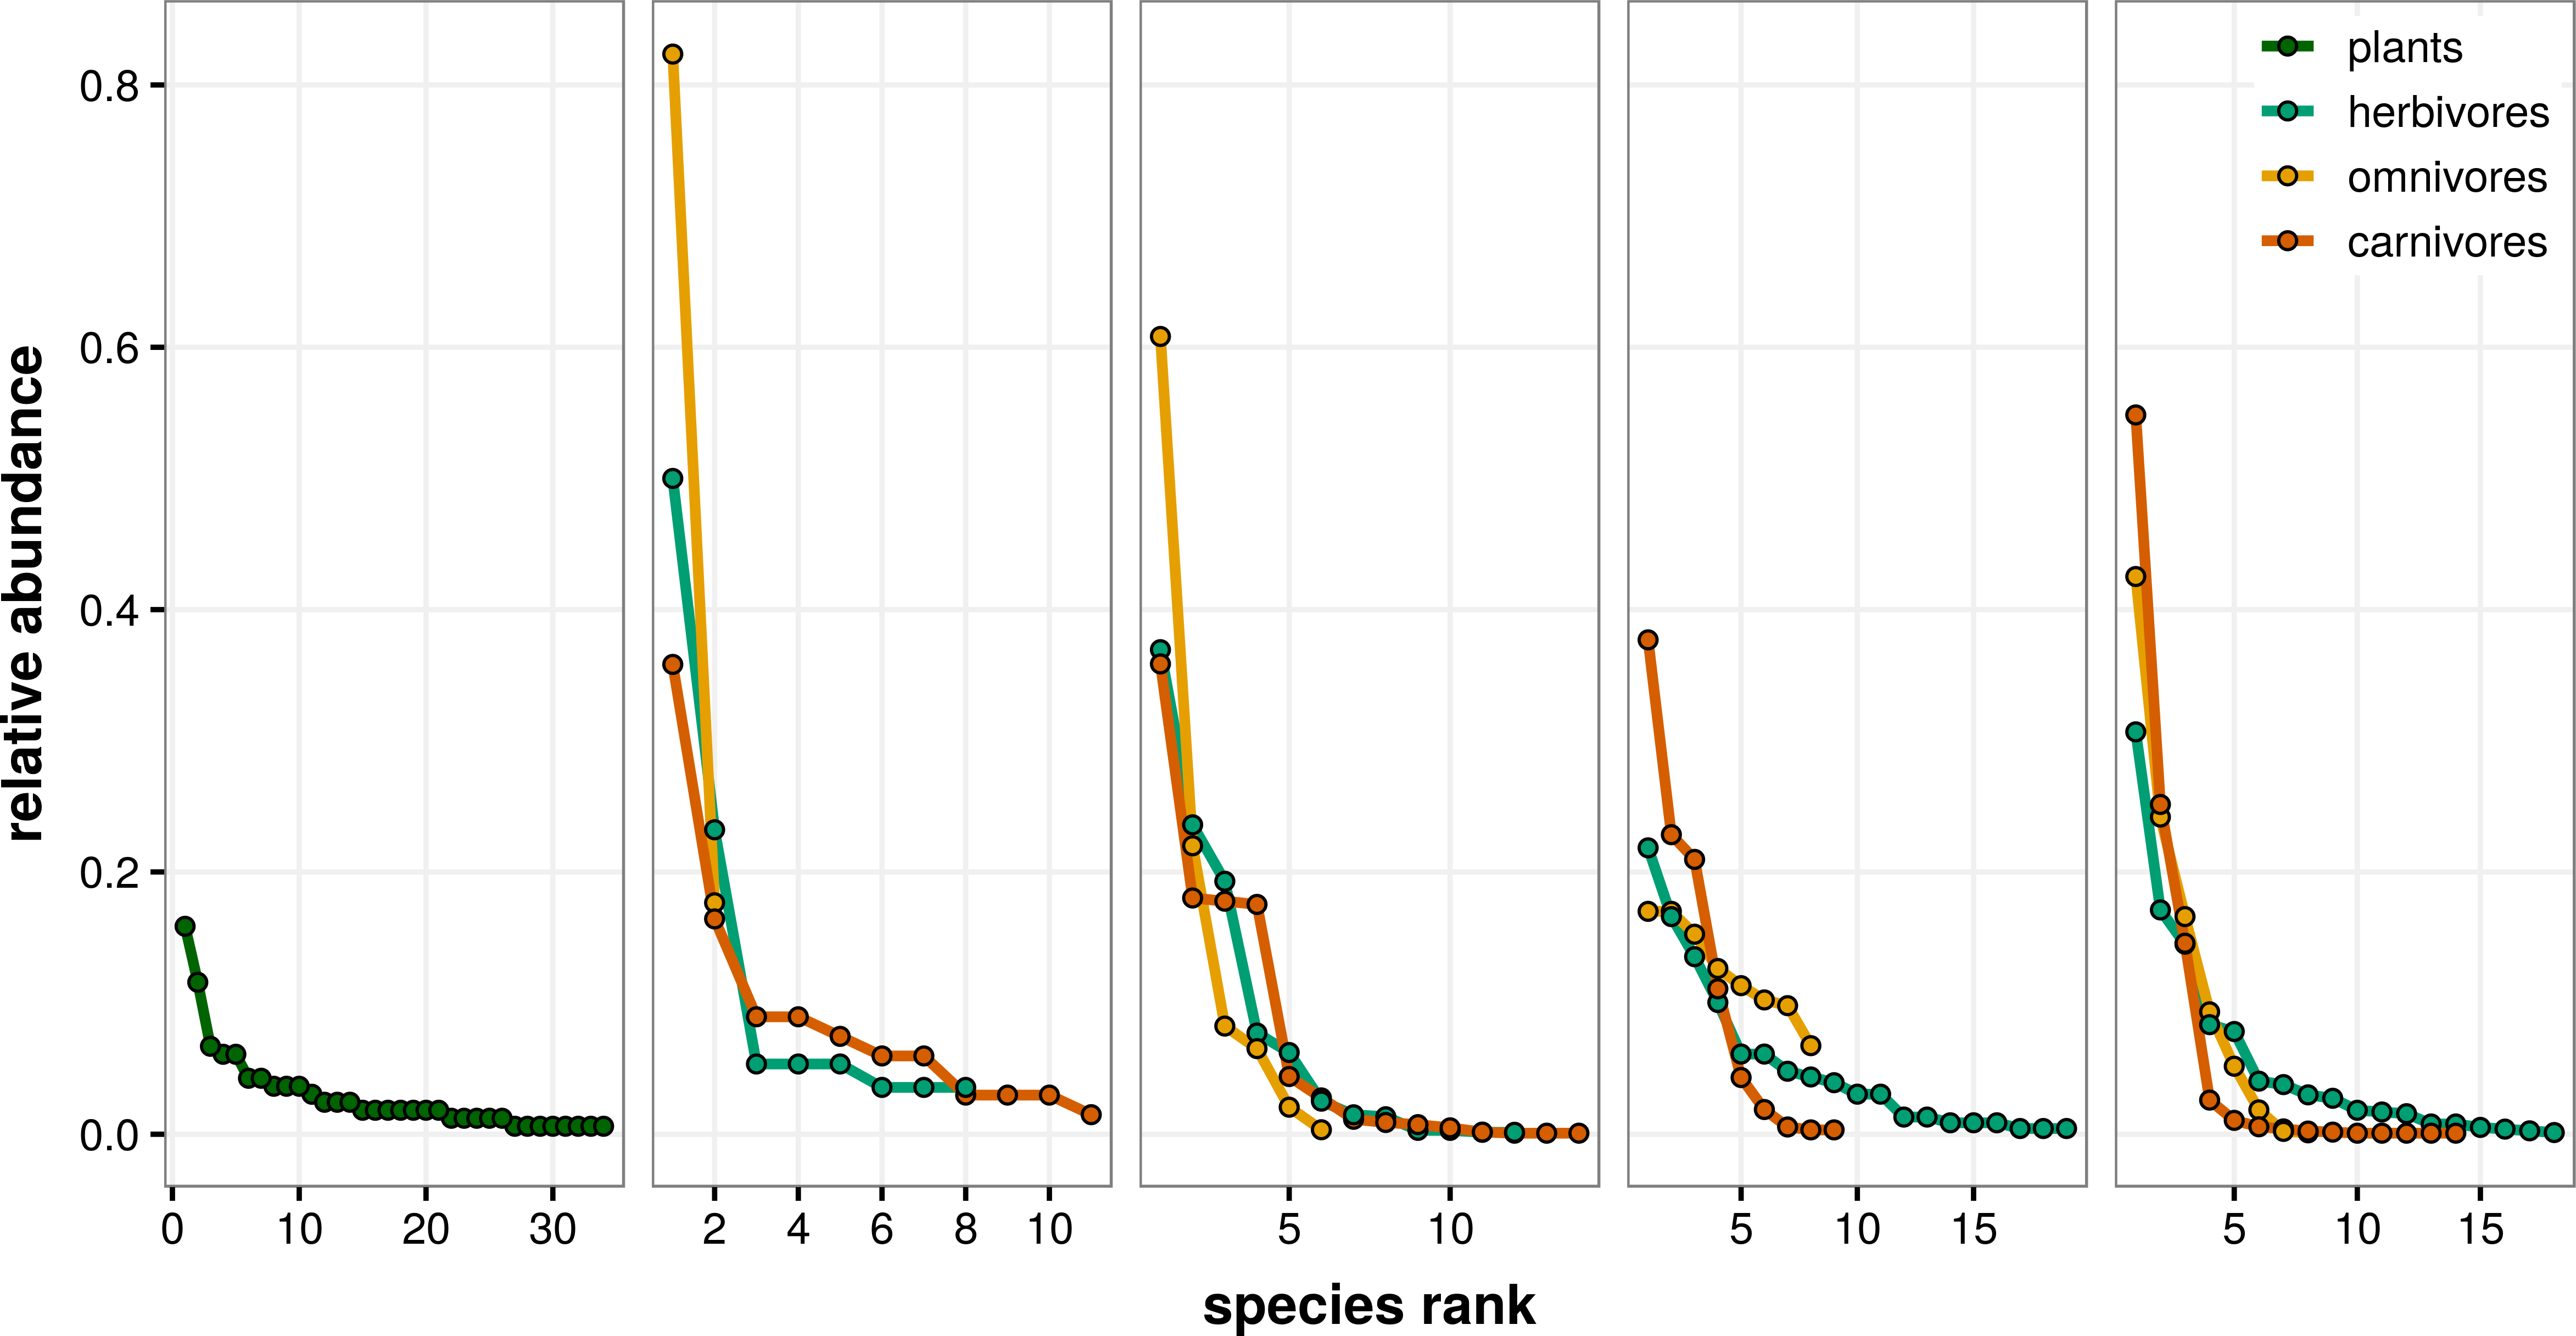
\includegraphics[width=\textwidth,height=\textheight,keepaspectratio]{./Figures/chapter04/Fig_2.png}
\caption[Five empirical rank-abundance curves]{\color{Gray}Rank-abundance curves for five sites of the empirical datasets. The leftmost panel shows a curve from a GENTRY site, the other four are sampling sites of the MCDB dataset. }\label{fig:fig4.2}
\end{figure}

\subsubsection*{Statistical analyses}

I calculated the evenness and skewness metrics of each guild at sites in which there are at least three species of that guild, in order to avoid potential biases (for example, a guild of a single species is completely even, or a guild of two species is never skewed). The variation of the SAD metrics with trophic guild was analyzed via statistical models. Evenness values are bounded within the interval [0,1], so a beta regression is an appropriate choice for modelling such bounded data, given the flexibility of the beta distribution. I transformed the evenness values in order to obtain data without proper zeroes and ones, i.e. bounded in (0,1), following \cite{Smithson2006}, and applied a beta regression with trophic guild, species richness, temporal extent and spatial extent as predictors. In particular, I used the R implementation of the GAMLSS family of models \citep{Rigby2005}, which allows probability density functions to be specified by any number of parameters, themselves functions of the independent variables. I modelled the evenness probability density function with two parameters $\mu$ and $\sigma$, named the \textit{location} and \textit{scale} parameters. These parameters are related to the parameterization of the beta distribution in terms of two shape parameters $\alpha$ and $\beta$ in the following way:

\begin{align}%\label{eq:eq4.3}
& \mu = \frac{\alpha}{\alpha + \beta} \\
& \sigma = \frac{1}{\alpha + \beta + 1}
\end{align}

Then, given a random variable $Y \sim D(\mu,\sigma)$, the mean and variance of the beta distribution in these terms is:

\begin{align}\label{eq:eq4.4}
& E(y) = \mu \\
& Var(y) = \sigma^2 * \mu * (1-\mu)
\end{align}

For the final model, I selected the link functions of $\mu$ and $\sigma$, and the final set of predictors, via AIC model selection.

Skewness presented a clearly bimodal distribution, with peaks at 0 and 1. Due to the difficulty of modelling such continuous bimodal data, I opted for categorizing the response into three levels of skewness: highly negative, low skewness, and highly positive, represented by the intervals [-1,-0.5), [-0.5,0.5], and (0.5,1]. This response was modelled via a multinomial regression with the same set of predictors as the evenness metric, and AIC model selection was also performed to obtain the final set of predictors.

For the MCDB dataset, it is common to observe species from two or more trophic guilds at the same site (Fig. \ref{fig:fig4.2}). It is therefore possible to calculate the rarity of each guild as the difference between its proportion of individuals and its proportion of species in the local communities \citep{Spencer2000}. Furthermore, to complement this calculation, I obtained the relative dominance value of each guild at each site, measured as the abundance of the most abundant species divided by the summed abundances of its guild \citep{Spencer2000, Dornelas2011}.

\section{Results}

\subsection*{Theoretical model}

Evenness and skewness metrics show contrasting responses to variations in trophic guild, richness and connectance (Tables \ref{tab:tab4.1} and \ref{tab:tab4.2}, see Fig. \ref{fig:fig4.3} for a subset of the results). After a high increase in evenness from primary producers to herbivores, the metric decreases on average with trophic guild. Likewise, richness displays a negative relationship with evennes, whereas connectance shows a more complex relationship, with minimum overall evenness observed at intermediate levels of connectance (Table \ref{tab:tab4.1}). Skewness, in turn, displays almost opposite trends: it increases with increasing trophic position, richness, and connectance (Table \ref{tab:tab4.2}).

\begin{figure}[htbp!]
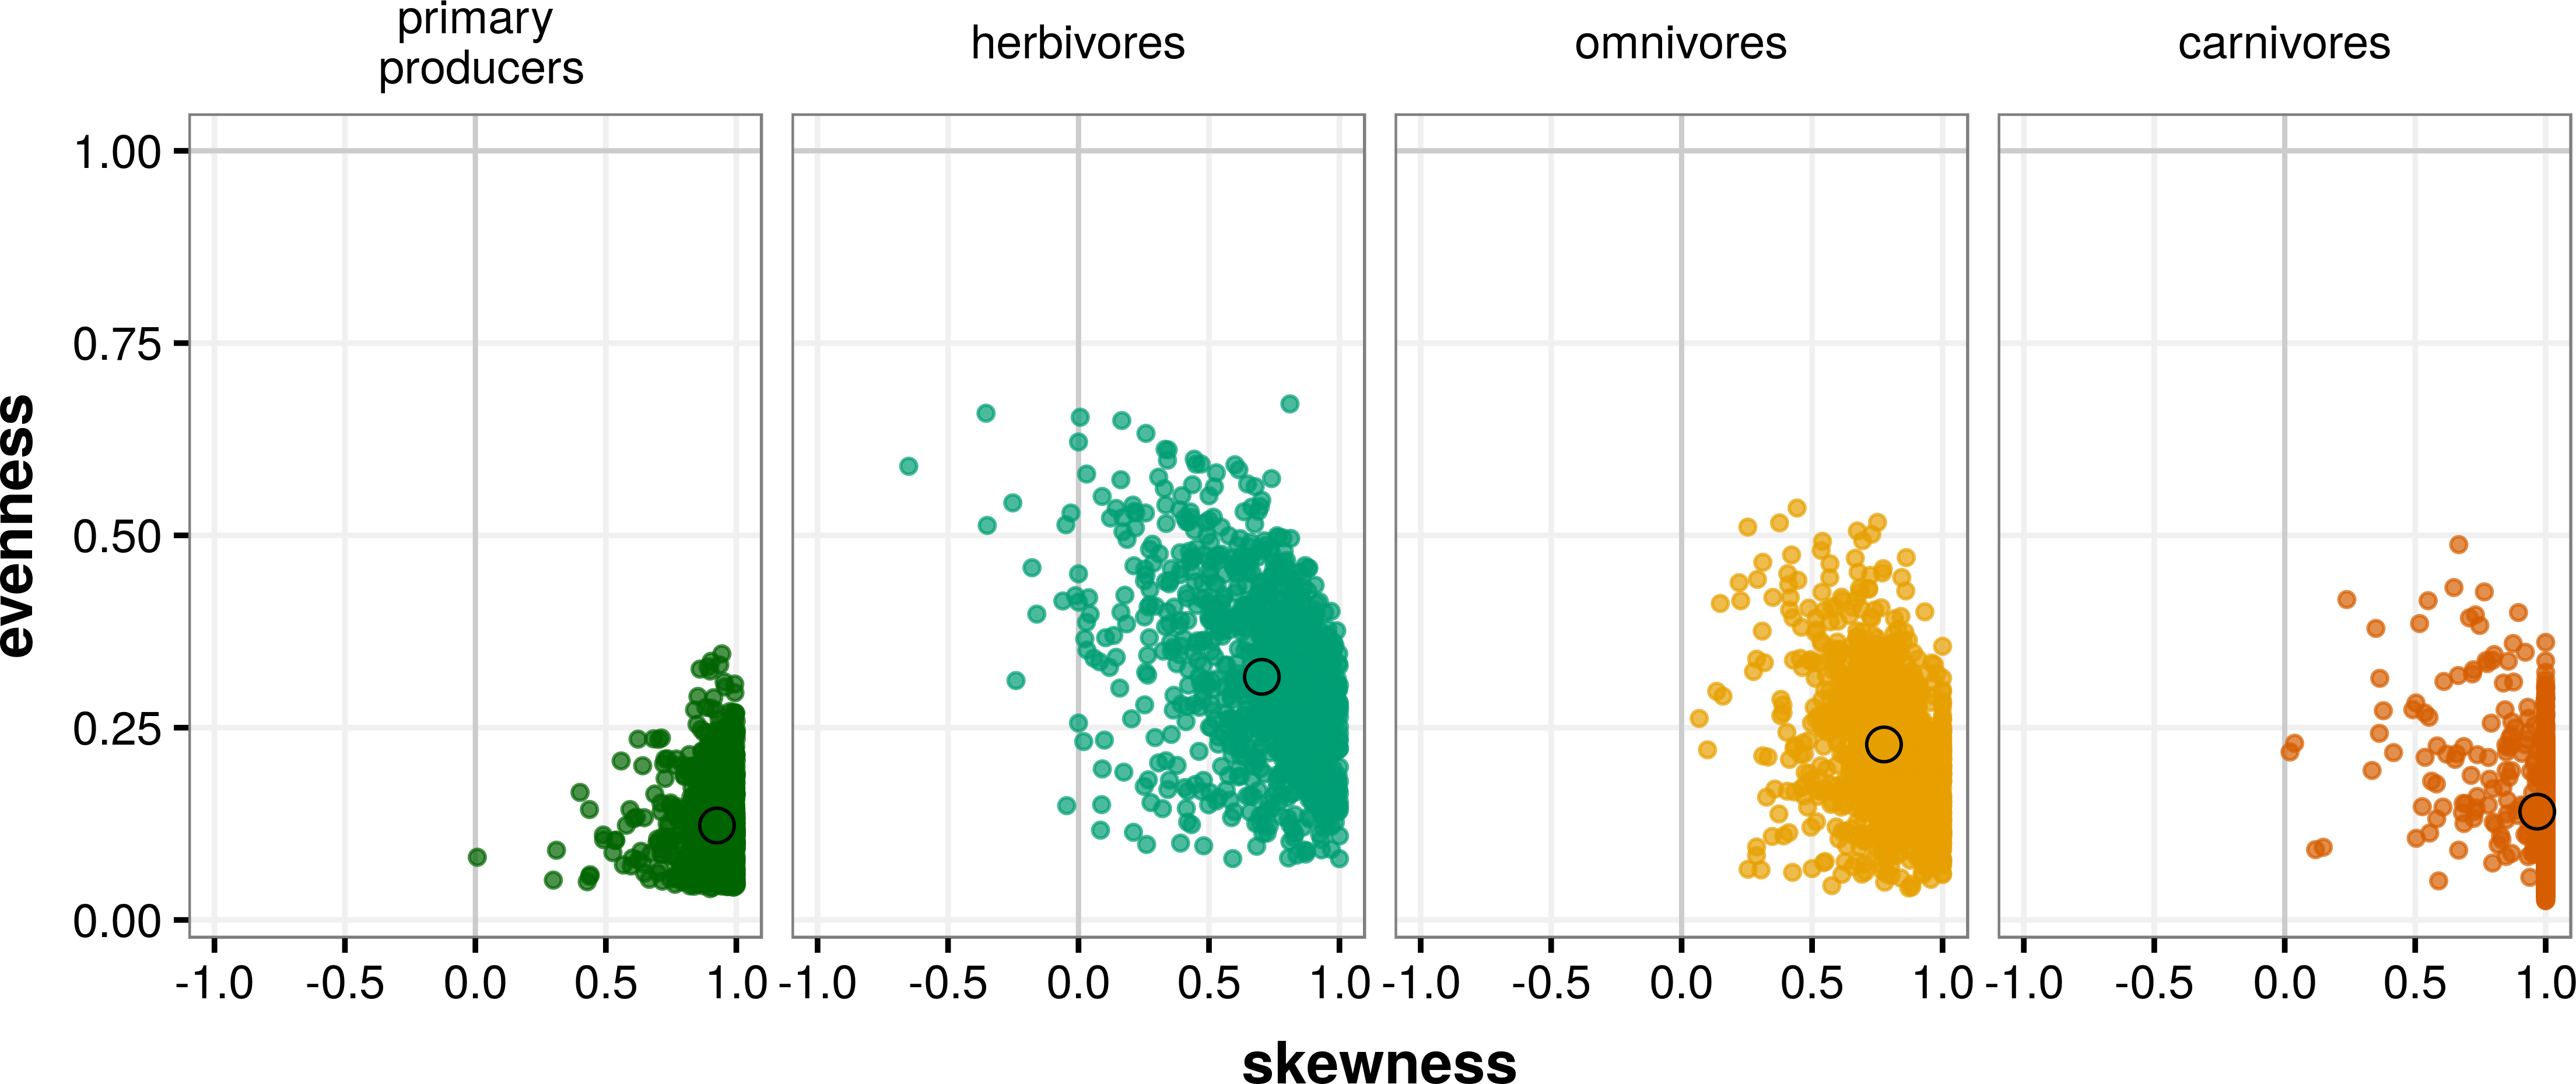
\includegraphics[width=\textwidth,height=\textheight,keepaspectratio]{./Figures/chapter04/Fig_3.png}
\caption[Model evenness and skewness]{\color{Gray}Evenness and skewness values for the trophic guilds of simulated networks. In this figure, each dot represents one realization of a network with richness = 100 and connectance = 0.2. Note that the abundances predicted by the model correspond to the three consumer levels, whereas abundances of primary producers are inputs to the model, and are shown for reference. Black circles represent the centroid of the two-dimensional distributions.}\label{fig:fig4.3}
\end{figure}

\begin{table}[ht!]
\centering
\caption[Coefficients from evenness regression in simulated networks]{\color{Gray}Estimated regression parameters, standard errors, t-statistic values and p-values for the mixed effect model \textit{evenness $\sim$ richness + connectance + trophic guild + random(replicate)} of the theoretical model. $\sigma_{replicate}$ is $5.3*10^{-8}$, and the $r^2$ of the model is 0.4}\label{tab:tab4.1}
\begin{tabular}{llllll}
\hline
Variable & Estimate & Std. Error &         df & t value & p-value \\
\hline
(Intercept)            &  0.41 & $1.848*10^{-3}$ & $2.63*10^{4}$ & 221.871 & $<0.05$ \\
richness-100      & -0.091 & $1.72*10^{-3}$ &  $2.63*10^{4}$ & -53.237 & $<0.05$ \\
richness-200      & -0.155 & $1.72*10^{-3}$ &  $2.63*10^{4}$ & -89.997 & $<0.05$ \\
connectance-0.2   & -0.007 & $1.7*10^{-3}$ &  $2.63*10^{4}$ & -4.351 & $<0.05$ \\
connectance-0.3   &  0.007 & $1.73*10^{-3}$ &  $2.63*10^{4}$ & 3.773 & $<0.05$ \\
trophic.guild-omnivores & -0.079 & $1.7*10^{-3}$ & $2.63*10^{4}$ & -46.453 & $<0.05$ \\
trophic.guild-carnivores & -0.167 & $1.73*10^{-3}$ & $2.63*10^{4}$ & -96.437 & $<0.05$ \\
\hline
\end{tabular}

\end{table}

\begin{table}[ht!]
\centering
\caption[Coefficients from skewness regression in simulated networks]{\color{Gray}Estimated regression parameters, standard errors, t-statistic values and p-values for the mixed-effects model \textit{skewness $\sim$  richness + connectance + trophic guild + random(replicate)} of the theoretical model. $\sigma_{replicate}$ is 0.0032, and the $r^2$ of the model is 0.24}\label{tab:tab4.2}
\begin{tabular}{llllll}
\hline
Variable & Estimate & Std. Error &         df & t value & p-value \\
\hline
(Intercept)       & 0.561 &  $3.65*10^{-3}$ & $1.9*10^{4}$ & 153.603 & $<0.05$ \\
richness-100      & 0.117 &  $3.39*10^{-3}$ & $2.5*10^{4}$ & 34.574 & $<0.05$ \\
richness-200      & 0.177 &  $3.4*10^{-3}$ & $2.5*10^{4}$ &  51.957 & $<0.05$ \\
connectance-0.2   & 0.019 &  $3.36*10^{-3}$ & $2.53*10^{4}$ &   5.674 & $<0.05$ \\
connectance-0.3   & 0.0048 &  $3.42*10^{-3}$ & $2.53*10^{4}$ &   1.414  &  0.157  \\
trophic.guild-omnivores & 0.086 &  $3.36*10^{-3}$ & $2.53*10^{4}$ &  25.739  & $<0.05$ \\
trophic.guild-carnivores & 0.253 &  $3.43*10^{-3}$ & $2.54*10^{4}$ &  73.909  & $<0.05$ \\
\hline
\end{tabular}

\end{table}

\FloatBarrier

\subsection*{Empirical datasets}

The statistical model for evenness included all the original predictors (trophic guild, richness, spatial extent and temporal extent, Table \ref{tab:tab4.3}). Plant guilds were the less even ones overall, showing significant differences with all other guilds (panel (a) of Fig. \ref{fig:fig4.4}, \cref{tab:tabApp4.1.4}). Among mammal guilds, herbivores show the highest average evenness, after which it further decreases with increasing trophic rank, although the differences are non-significant (\cref{tab:tabApp4.1.4}). This overall pattern of a significant increase from primary producers to consumers followed by a sustained decrease is qualitatively similar to the patterns obtained with the theoretical model, although the evenness values of the theoretical model are much lower than those of the empirical datasets (compare Figs. \ref{fig:fig4.3} and \ref{fig:fig4.4}). Richness has a positive effect on evenness, while also decreasing its variability (compare the sign of $\mu$ and $\sigma$ richness parameters), whereas increasing temporal and spatial extent has a negative effect on mean evenness, and no effect on its variability (Table \ref{tab:tab4.3}).

\begin{figure}[ht!]
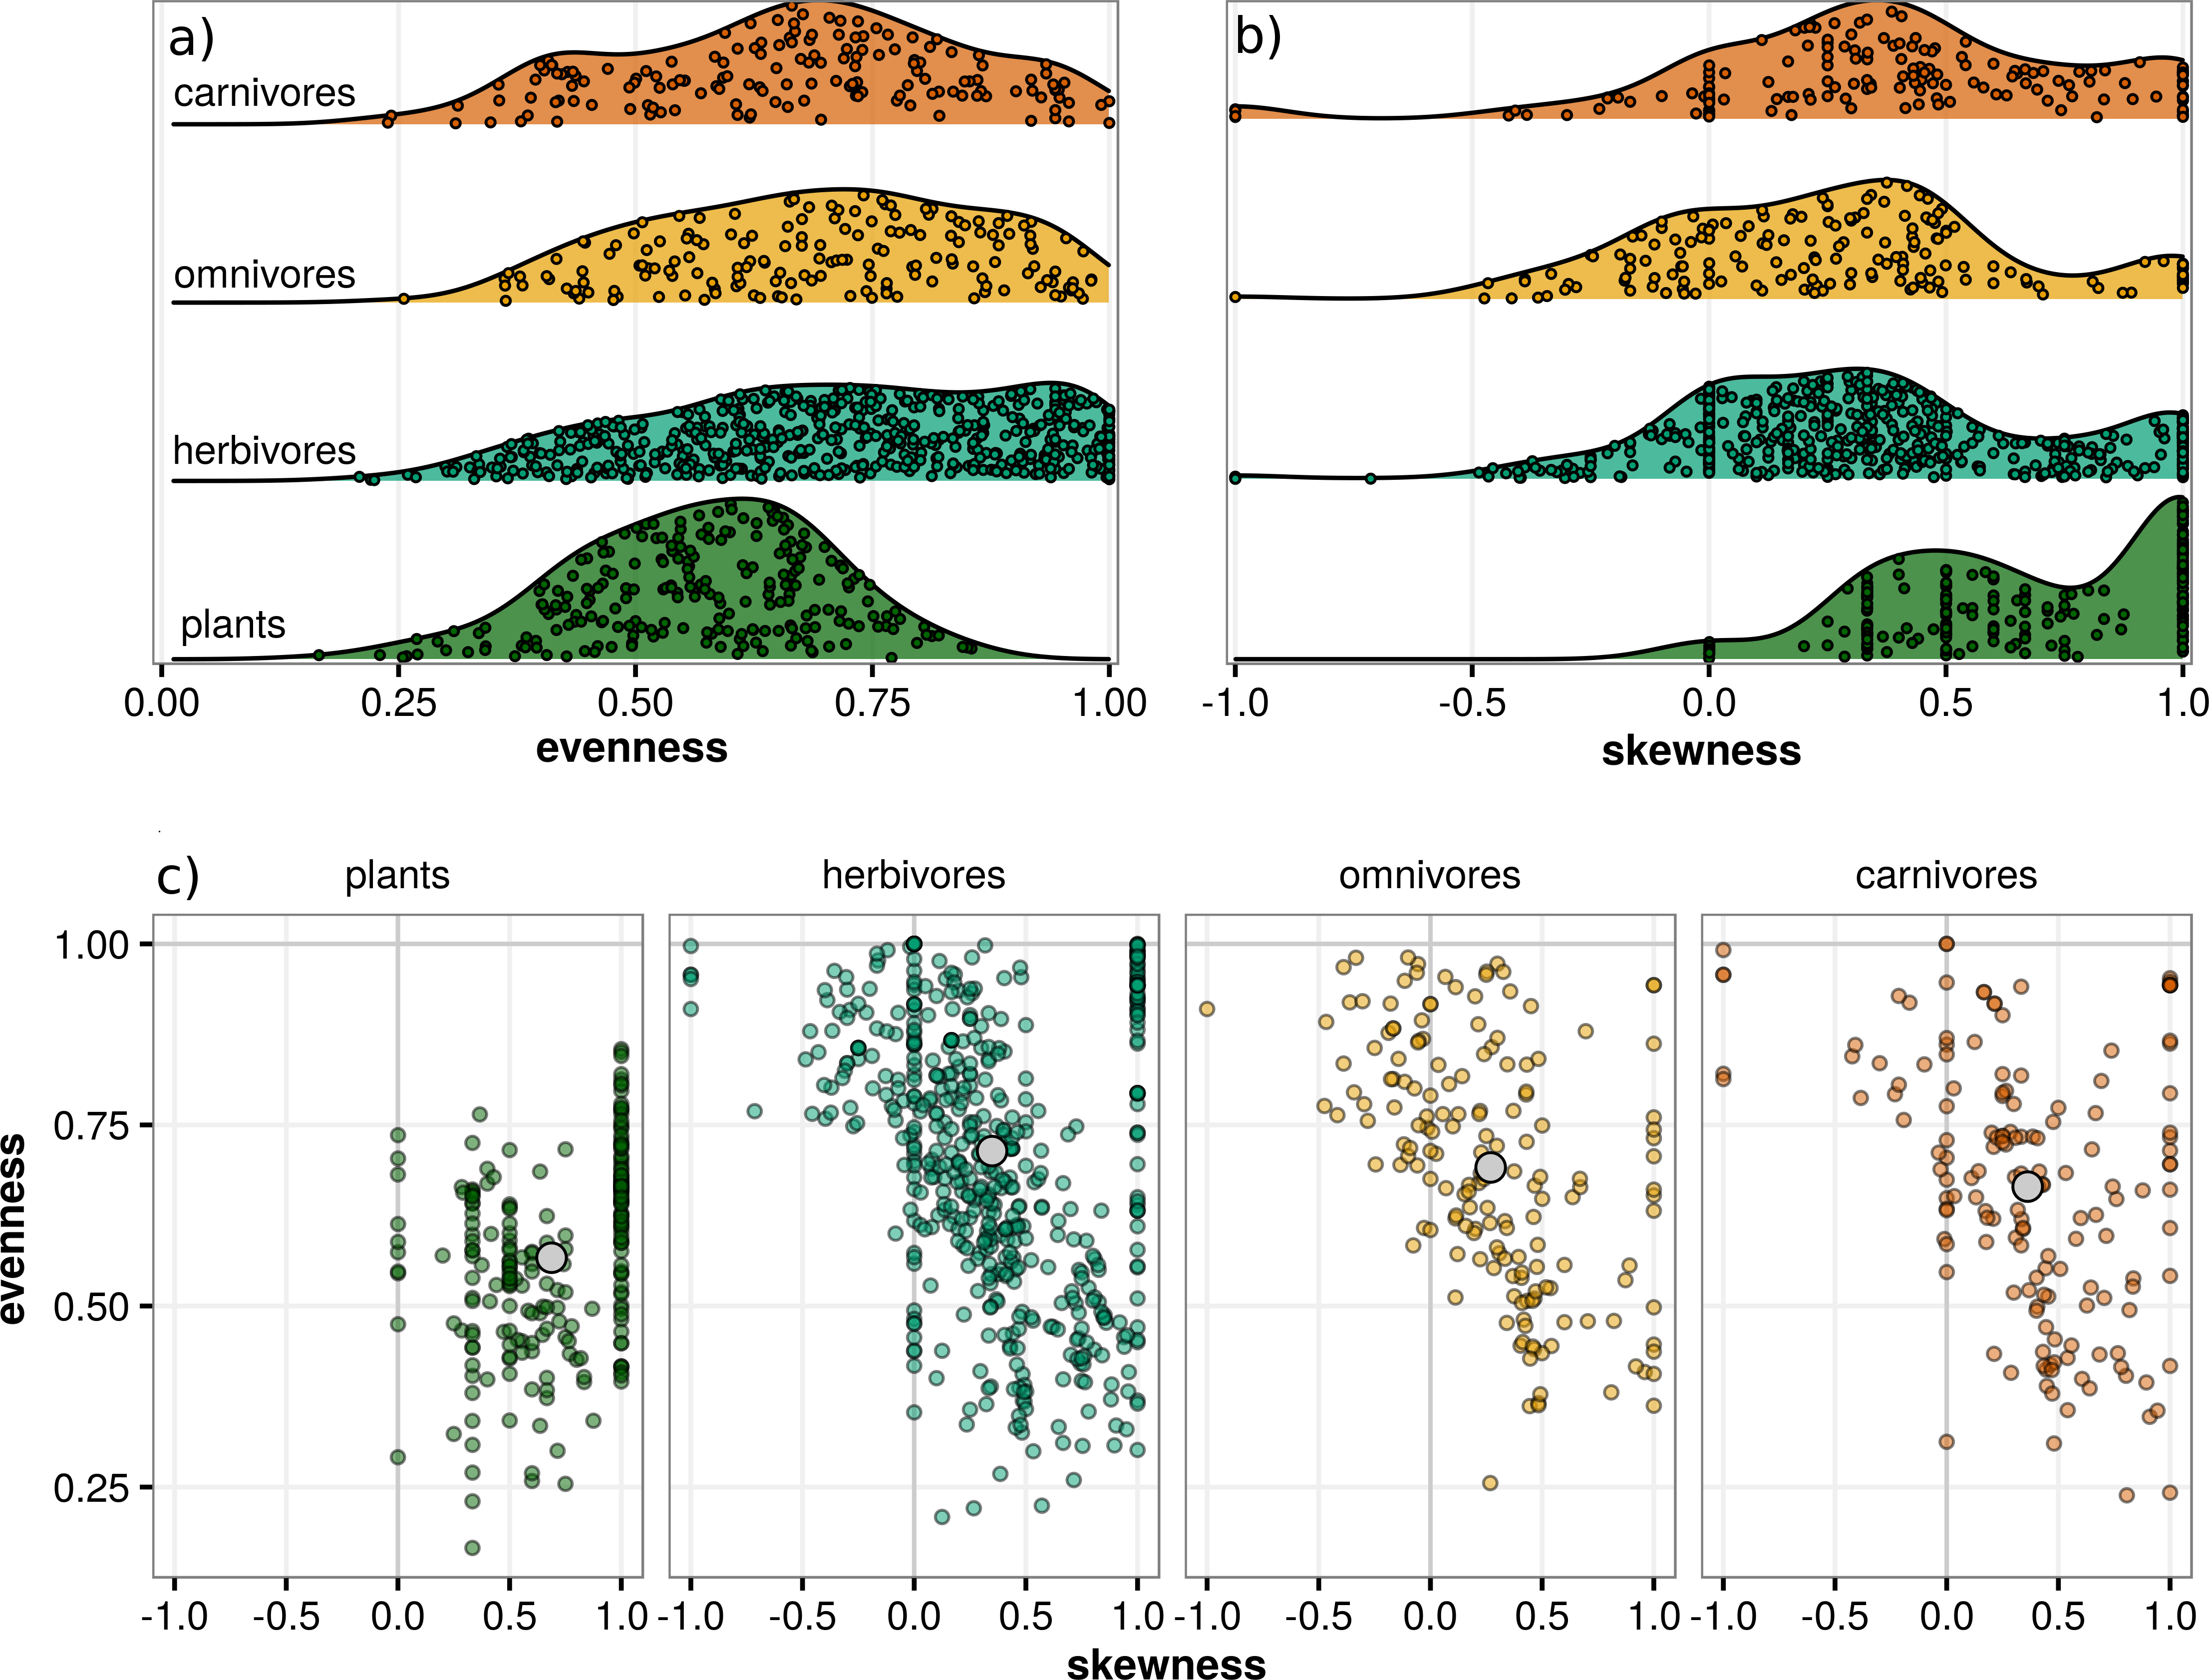
\includegraphics[width=\textwidth,height=\textheight,keepaspectratio]{./Figures/chapter04/Fig_4.png}
\caption[Evenness and skewness in empirical guilds]{\color{Gray}Density distributions of evenness (a) and skewness (b) values of the guilds studied, and the combined distribution of both metrics (panel c, cf. the theoretical results of Fig \ref{fig:fig4.3}).}\label{fig:fig4.4}
\end{figure}

\begin{table}[htbp!]
\centering
\caption[Evenness model coefficients]{\color{Gray} statistical model coefficients for the evenness of the empirical datasets. See the main text for explanation of the $\mu$ and $\sigma$ parameters. The $r^2$ of the overall model is 0.39}\label{tab:tab4.3}
\begin{tabular}{lllll}
\hline
Variable & Estimate & Std. Error & t value & p-value \\
\hline
\textbf{$\mu$ link function:  cloglog} & & & &  \\
(Intercept)              & -0.509 & 0.039 & -12.824 & $<0.05$ \\
trophic.guild-herbivores   &  0.8681 & 0.055 & 15.882 & $<0.05$ \\
trophic.guild-omnivores    &  0.753 & 0.062 &  11.975 & $<0.05$ \\
trophic.guild-carnivores    &  0.711 & 0.069 & 10.382 & $<0.05$ \\
spatial.extent           & $-7.8*10^{-7}$ & $3.1*10^{-7}$ & -2.481 & $<0.05$ \\
temporal.extent          & $-3.8*10^{-3}$ & $1.3*10^{-3}$ & -2.914 & $<0.05$ \\
richness                 &  $3.2*10^{-3}$ & $2.6*10^{-4}$ & 12.126 & $<0.05$ \\
\hline
\textbf{$\sigma$ link function:  logit} & & & & \\
(Intercept)              & -0.98 & 0.106 & -9.273 & $<0.05$ \\
trophic.guild-herbivores   &  0.969 & 0.117 &  8.251 & $<0.05$ \\
trophic.guild-omnivores    &  0.461 & 0.135 &  3.407 & $<0.05$ \\
trophic.guild-carnivores   &  0.819 & 0.143 &  5.709 & $<0.05$ \\
spatial.extent            &$-1.4*10^{-7}$ & $3.9*10^{-7}$ & -0.359 & 0.719 \\
temporal.extent           &$-6.1*10^{-4}$ & $1.5*10^{-3}$ & -0.401 & 0.688 \\
richness                  &$-3.1*10^{-3}$ & $8.6*10^{-4}$ & -3.624 & $<0.05$ \\
\hline
\end{tabular}

\end{table}

The final model for skewness included trophic guild and richness as the only predictors. Again, there were significant differences between plant and mammal guilds in their average skewness (Table \ref{tab:tab4.4}). Plant and mammal guilds were different mainly when considering low and positive skewness levels, where plants showed the highest average skewness, followed by a drop in all mammal guilds, which showed no statistical differences (Fig. \ref{fig:fig4.4}, \cref{tab:tabApp4.1.5}). Again, a similar qualitative trend is observed in the theoretical model (Fig. \ref{fig:fig4.3}). The effect of richness is positive, but only significant for the variation between low and highly positive skewness values (Table \ref{tab:tab4.4}).

\begin{table}[htbp!]
\centering
\caption[Skewness model coefficients]{\color{Gray} statistical model coefficients for the skewness of the empirical datasets. The $r^2$ of the model is 0.15}\label{tab:tab4.4}
\begin{tabular}{llllll}
\hline
Variable & category & Estimate & Std. Error & z score & p-value \\
\hline
(Intercept)              & (0.5,1] & -0.038 & 0.268 & -0.143  & 0.88 \\
                         & [-1,-0.5) & -5.773  & 0.688 & -8.39 & $<0.05$ \\
trophic.guildherbivores   & (0.5,1] & -0.882 & 0.276 & -3.198 & $<0.05$ \\
                         & [-1,-0.5) & 3.138 & 0.478 & 6.571 & $<0.05$ \\
trophic.guildomnivores    & (0.5,1] & -1.492  & 0.342 & -4.362 & $<0.05$ \\
                         & [-1,-0.5) &  2.322 & 0.788 & 2.946  & $<0.05$ \\
trophic.guildcarnivores    & (0.5,1] & -0.832 & 0.327 & -2.548 & $<0.05$ \\
                         & [-1,-0.5) & 4.354 & 0.492 & 8.854 & $<0.05$ \\
richness                 & (0.5,1] & 0.012 & 0.003 & 4.427   & $<0.05$ \\
                         & [-1,-0.5) & -0.314 & 0.224  & -1.397 & 0.16 \\
\hline
\end{tabular}

\end{table}

\FloatBarrier

The three mammal trophic guilds show similar negative correlations between dominance and richness (panel (a) of Fig. \ref{fig:fig4.5}, Pearson's $\rho$: -0.62 for herbivores, -0.66 for omnivores, -0.64 for carnivores). Regarding the relative rarity of the different guilds (panel (b) of Fig. \ref{fig:fig4.5}), herbivores have the same proportion of species than of individuals in local communities (Wilcoxon signed-rank test, $W = 131422, p = 0.14$, \cref{tab:tabApp4.1.6}), whereas omnivores are comparatively more common (i.e. there are higher relative numbers of omnivore individuals than species, $W = 162226, p < 0.05$) and carnivores are rarer (there are more carnivore species than individuals, $W = 18772, p < 0.05$).

\begin{figure}[ht]
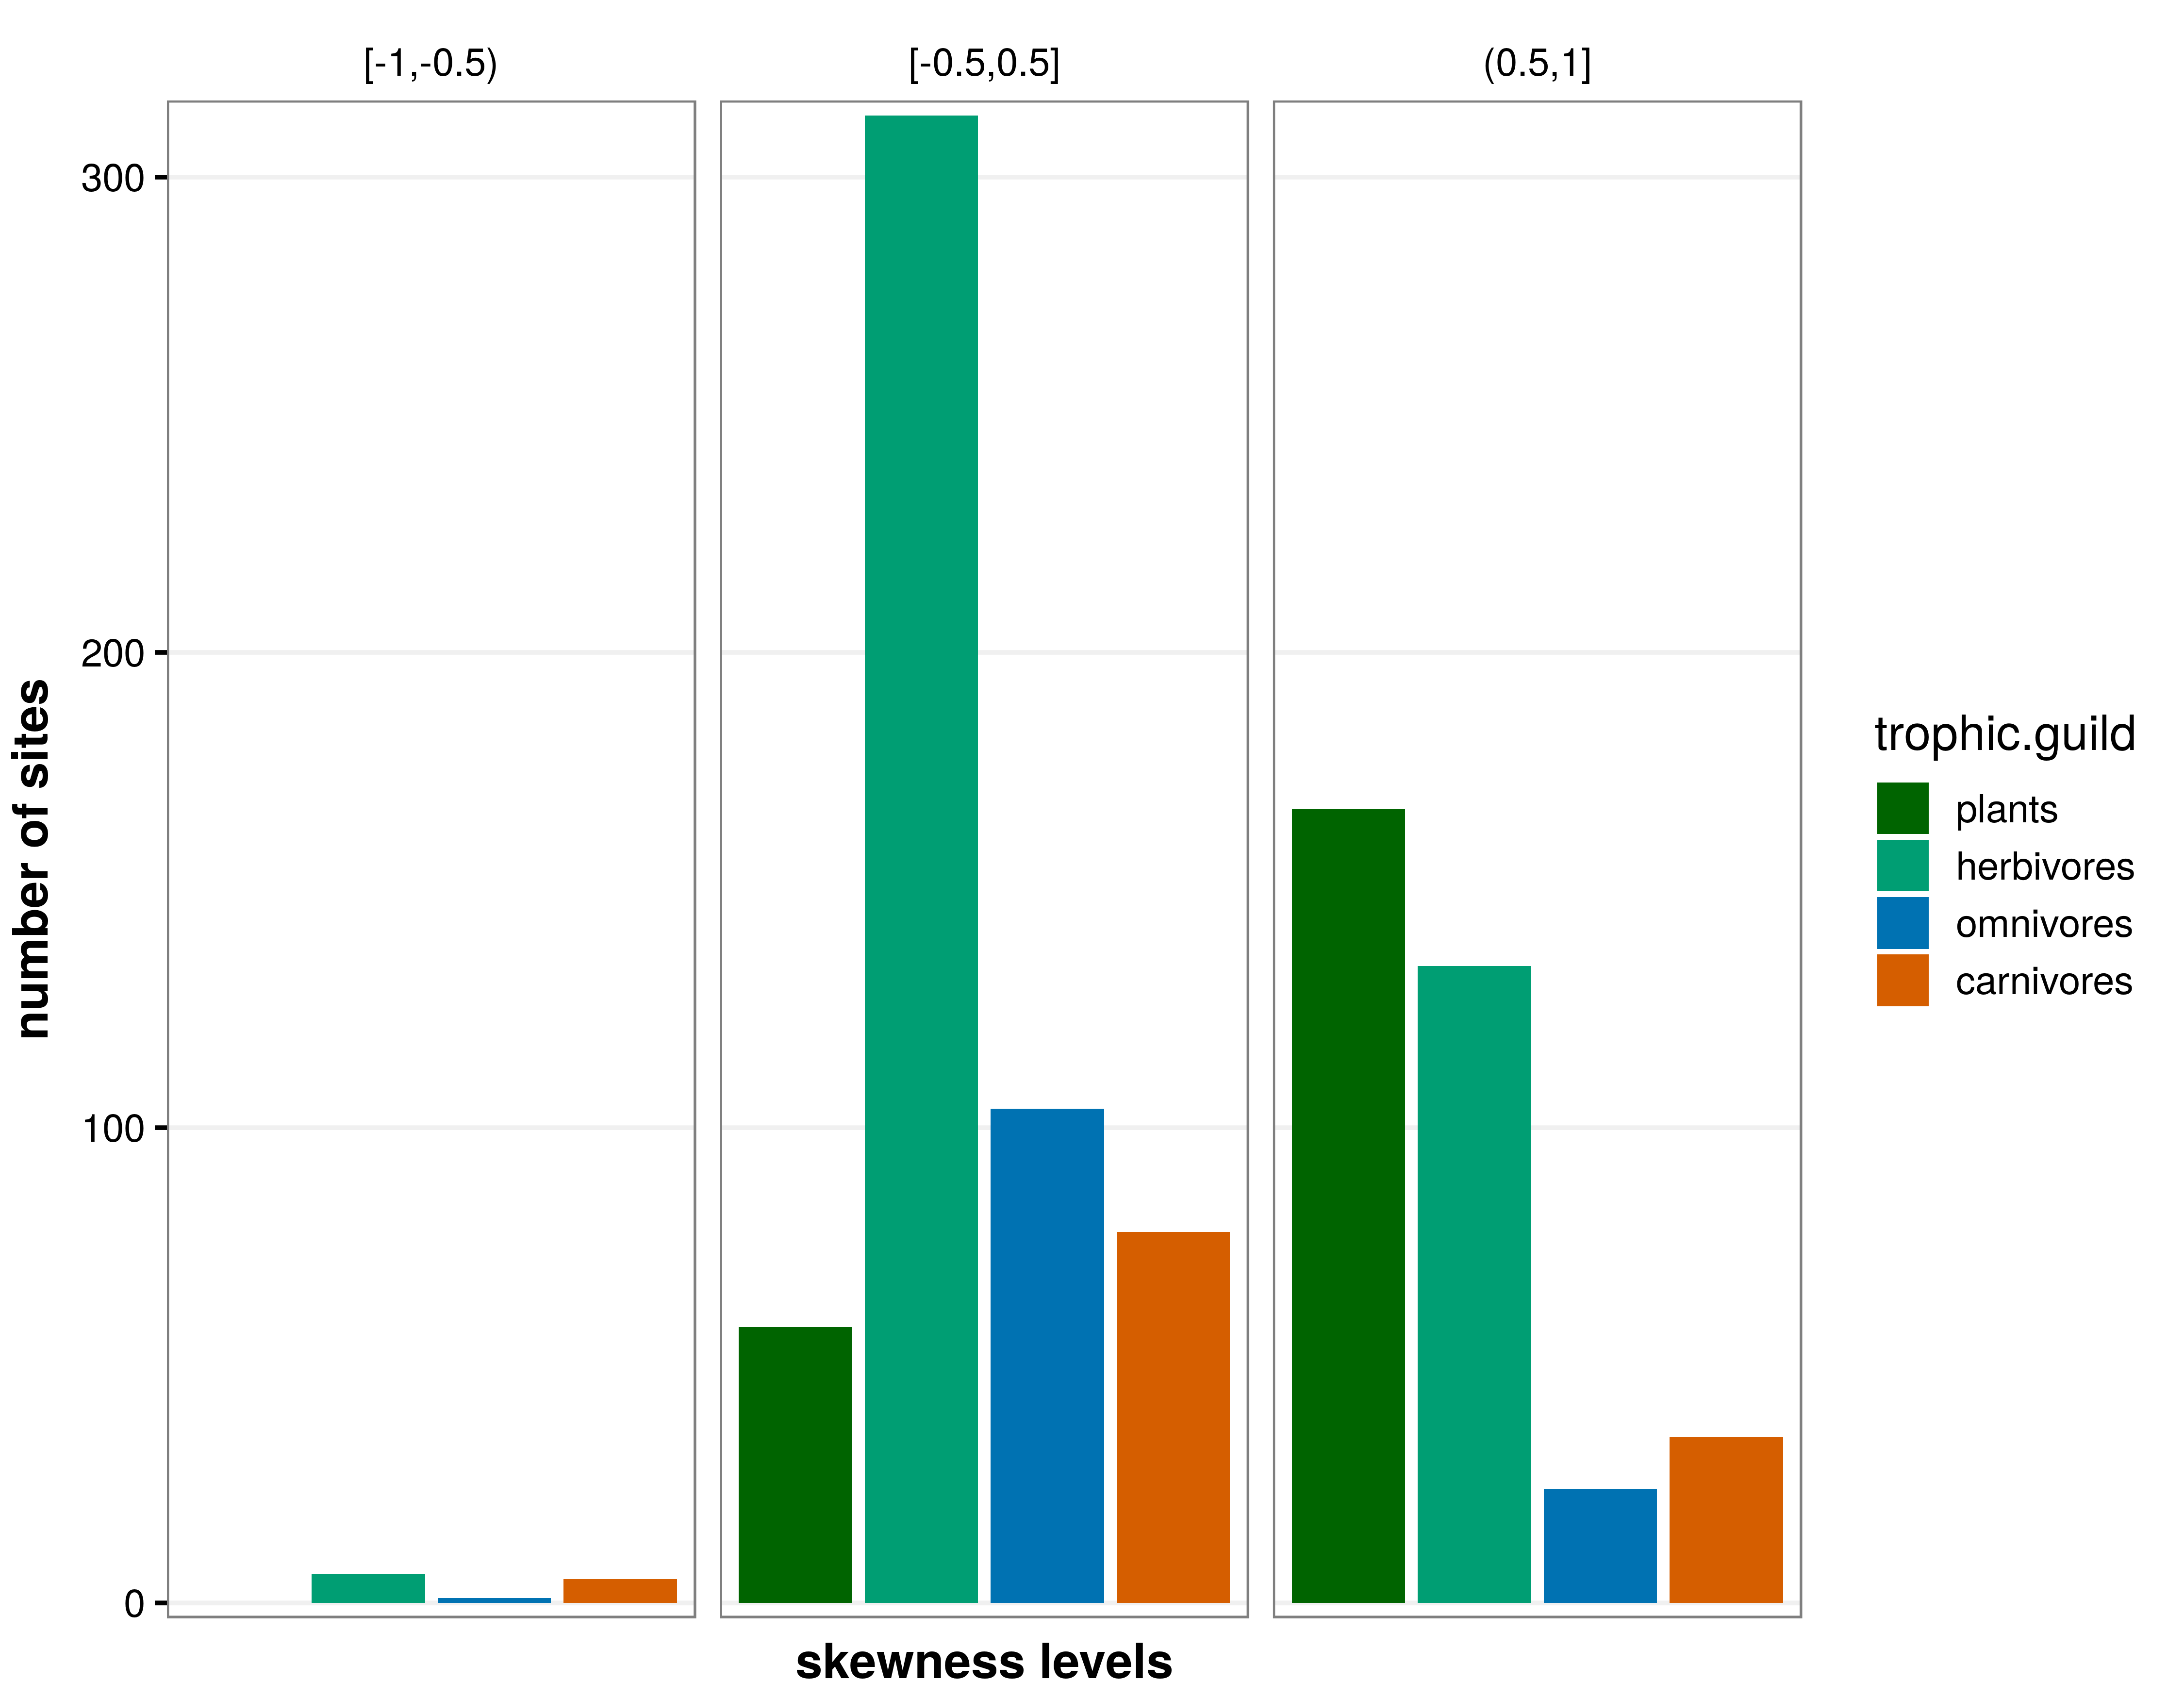
\includegraphics[width=\textwidth,height=\textheight,keepaspectratio]{./Figures/chapter04/Fig_5.png}
\caption[Species/indiv. proportion and dominance in guilds]{\color{Gray} Patterns of dominance, and the proportion of species and individuals of the mammal guilds across sampling sites, where each point is a sampling site. Dominance (upper panel) is defined as the number of individuals of the most abundant species in the guild relative to all individuals from that guild. Minimum and maximum potential dominances are represented by solid curves. The maximum level of richness shown here, for visibility, is 20 species. The lower panel shows the proportion of individuals of a given guild against the proportion of species of the same guild, and the x=y line is shown for visibility. Grey-colored dots in both panels represent average values.}\label{fig:fig4.5}
\end{figure}

\section{Discussion}

In local communities, the division of species in trophic guilds is informative with regards to the distribution of interactions and biomass flows in the community \citep{Lindeman1942, Kefi2016a}, but everything else being equal, it is unclear wheter SAD metrics are influenced by the trophic position of a guild in the local community. Here I have shown that there are significant differences between the local SADs of terrestrial plant guilds (primary producers) and different guilds of terrestrial mammals, with plant SADs being less even and more skewed than mammal ones. Furthermore, the empirical relationship between SAD metrics and trophic guild is also mediated by species richness and the spatiotemporal extent of the sample. A theoretical model combining network structure and niche apportionment schemes shows qualitatively similar trends in the variability of SAD shape across trophic guilds.

There are several potential ways of generating theoretical predictions about the variability of SAD metrics with trophic guild. Recent extensions to the theory of island biogeography \citep{Holt2009a, Gravel2011} make explicit the differences and feedbacks between species in discrete food chains, and could potentially be extended to predict the variability in species abundances across trophic levels. The model presented here, in turn, is meant to explore the role of local community structure in communities with a fixed number of species and no dynamic migration. In particular, the main question behind it is to explore whether variations in community structure (represented by species richness and network connectance) influence SAD shape of the increasing trophic guilds in model food webs.

I have shown that, given the assumptions of the model, evenness is highest (and skewness lowest) for herbivore species, and decreases for omnivore and carnivore guilds. Furthermore, community structure has significant impacts on both metrics: both richness and connectance have generally negative effects on guild evenness, and positive effects on the skewness of the SAD. With increasing richness or connectance, there is an associated increase in the number of trophic links for each species (its degree), so the general explanation for these patterns is that, under random fraction apportionment of resources, higher levels of resource overlap of the species within a given trophic guild drive higher heterogeneity in abundance distributions. Other niche apportionment schemes are likely to display different abundance patterns. For example, the \textit{dominance preemption} scheme tends to produce highly heterogeneous distribution of resources and greater dominance levels than the random fraction apportionment. On the other hand, the \textit{dominance decay} scheme will generate increasingly even abundance distributions with increasing richness or connectance \citep{Tokeshi1990}.

The empirical datasets analyzed here differ from the theoretical model in several fundamental aspects. Importantly, these datasets are likely to represent open communities, in which both core and transient species are observed, which has important implications for the associated SAD \citep{Magurran2003}. Furthermore, they are not derived from entire communities sampled across trophic guilds, but are rather a compilation in which species are classified afterwards into broad guilds (see Methods). Therefore, analogies between the theoretical results and the empirical patterns should be approached with caution, due to these important confounding factors. However, the qualitatively similar variation of SAD metrics with trophic guild observed in theoretical (Fig. \ref{fig:fig4.3}) and empirical data (Fig. \ref{fig:fig4.4}) could also be due to empirical guilds displaying, on average, mechanisms of niche apportionment similar to the ones modelled. If we assume as a working hypothesis that some degree of niche preemption by dominant species takes place \citep{Sugihara2003}, the lower evenness and higher skewness observed in terrestrial plant communities relative to mammal ones may be explained by differences in the set of resources available to the different guilds. In particular, competitive exclusion may be higher in plant communities, leading to higher dominance of a few species, due to the comparatively small set of resources for which plants compete (light, water, and essential nutrients, \citealt{Austin1990}). Mammal guilds, in turn, may potentially have a wider variety of resources available. For example, mammal herbivores, as classified in this study and according to the \textit{EltonTraits} database used to categorize trophic guilds \citep{Wilman2014}, can feed mainly on either seeds, fruits, nectar, pollen, and a large list of other plant parts. Therefore, a high degree of specialization within a guild may reduce the importance of competition and, subsequently, the relative differences in abundance between species \citep{Sugihara2003}. Such high specialization in trophic guilds is commonly observed in ecological networks \citep{Dunne2002, Gravel2011}.

Other complementary reasons for explaining the variation in SAD metrics between plants and mammals may exist. For example, differences in traits such as movement potential, which can make rare mobile mammal species harder to document, or unavoidable sampling inconsistencies between studies. It may also be the case that plant species are able to maintain lower densities for longer periods than mammal species, thus being more easily observed. Empirical estimates of minimum viable populations indicate that some plant populations may be viable with sizes of $< 1000$ individuals \citep{Nantel1996}, a number much lower than standard estimates for the viability of vertebrate species, which range in a few thousands of individuals \citep{Reed2003}. Therefore, there may simply be more rare plant species than mammals'. Niche differentiation may also be invoked to explain the relative homogeneity in SAD metrics between mammal guilds. As it is the case with herbivores, both omnivore and carnivore guilds may utilize a wide set of resources that may, generally, prevent a high degree of competitive exclusion.

Mammal guilds also show a negative correlation between dominance and guild richness, suggesting that richer guilds may be generally more even via a decrease in relative dominance, a result in accordance with previous studies \citep{Spencer2000,Dornelas2011}. This results contrast with the theoretical model, in which evenness and richness are negatively correlated (Table \ref{tab:tab4.1}). In empirical communities, the positive richness-evenness relationship may be due to the higher habitat complexity observed in richer communities \citep{Hurlbert2004}, a factor not included in the model that may lead to more diverse sets of resources and thus less importance of competitive exclusion. However, a negative relationship between richness and evenness has also been documented in different trophic guilds of grassland ecosystems \citep{Bock2007}. These contrasting results emphasize the need for controlled observations across different ecosystem types and productivity gradients. The only significant difference between mammal guilds found in this study is the relative rarity of carnivore species compared to those of other guilds, which also corroborates earlier results by \cite{Spencer2000} on invertebrate communities. Overall, these broad-scale results will undoubtedly vary across habitat types, depending on the specific sets of resources available to each guild, and on the local environmental conditions, which may have contrasting effects on the different trophic guilds \citep{Voigt2003}.

All the results presented here assume that trophic interactions are the main driver of variation in species abundances across guilds. In the theoretical results, bottom-up energy flows from trophic interactions are the only ones considered, and the mammal communities were grouped considering only a general trophic guild classification of the species. This approximation is clearly a simplification of the complex networks of interactions observed in nature, which may generate strong top-down or indirect feedbacks \citep{Menge1995, Montoya2009a}. The persistence and abundance of all species in a community is further influenced by the whole set of interactions in which they engage, among other factors \citep{Pocock2012, Garcia-Callejas2018a}. However, the distribution and frequency of most non-trophic interactions in empirical communities is not known, so no hypothesis can be formulated at this point regarding their influence on local SADs. In communities in which non-trophic interactions are known, functional guilds can be differentiated by accounting for the set of all interactions in which they engage rather than just trophic ones \citep{Sander2015,Kefi2016a}; this functional grouping may further reduce intraguild functional variability and thus increase across-guild differences, better reflecting differences in SAD shape across guilds. On the other hand, there is virtually an unlimited number of functional guilds in nature, and establishing a general, cohesive, and manageable set of functional guilds that can be applied to group every potential community seems unfeasible for the time being. Therefore, grouping by trophic guild represents a compromise between generality (as every community can be divided in such manner) and intraguild versus across-guild variability. In any case, the variability in SAD metrics across trophic guilds of a community, and its relationship with other factors, would be better explored with dedicated sampling campaigns of different trophic guilds in multi-trophic communities, in which properties such as trophic specialization can also be tracked. This could be carried out, for example, in pond mesocosms in which most species are confined to the pond habitat, or for terrestrial habitats, in small islands where complete censuses of different trophic guilds are feasible.

The existence of an intrinsic variability in SAD shape across functional guilds has important consequences for both fundamental and applied community ecology. In theoretical models, the contributions of intraguild and interguild interactions need to be integrated in a general mechanistic framework, in order for their relative importance to be estimated. This shift from intraguild, competitive interactions to multi-trophic, community scale thinking is a necessary step forward in theoretical community ecology \citep{Chesson2008,Godoy2018,Seibold2018}. Empirical analyses of SADs would also benefit from incorporating information about the communities that harbor the guilds under study. In studies analyzing intraguild drivers of SAD shape, the community context of the study should be used to establish null expectations of interguild influence, for example, based on network structural patterns. If the guilds under study are not functionally homogeneous (e.g. taxonomic assemblages sensu \citealt{Fauth1996}) deriving mechanistic explanations about SAD shape is usually not possible, due to interspecific differences in resource use, trophic position, etc. In such descriptive studies, therefore, the community context is unnecessary. Meta-analyses of Species Abundance Distributions have shown great disparity regarding the most appropriate statistical models for fitting SADs \citep{Ulrich2010,Baldridge2016}. If the results presented here hold, accounting for this null expectation may help clarify which statistical models are best suited to fit each set of data.

\section{Conclusions}

Species Abundance Distributions have many axes of variability. Here I have showed that intrinsic differences exist between the SAD of terrestrial plant and mammal communities. Plant communities are significantly less even and more skewed than mammal ones, and there are no significant differences in either metric between the mammal trophic guilds considered. This result may arise from differences in niche availability for the different guilds, following the hypothesis that higher niche availability implies a higher evenness in species abundances. Although these results are derived from extensive datasets controlling for several factors, targeted studies are needed to further confirm this pattern and test it in a variety of systems. This prospective line of research would shed new light on both theoretical and applied analyses of Species Abundance Distributions, and would help in the integration of classic horizontal community ecology patterns in the context of communities encompassing multiple trophic levels and interaction types.

%-----------------------------------------------------------------

%%************************************************
\chapter[Spatial propagation of interactions]{Spatial trophic cascades in communities connected by dispersal and foraging}\label{ch:spatial}
%************************************************

\tikz[remember picture,overlay] \node[opacity=0.3,inner sep=0pt] at (current page.center){\includegraphics[width=\paperwidth,height=\paperheight]{./Figures/cover/crow_1.jpg}};
\clearpage

\section*{Abstract}

The effects of pairwise interactions have indirect consequences that reverberate throughout the whole ecosystem. In particular, interaction effects may propagate in a spatial dimension, to localities connected by organismal movement. Here we study the propagation of interaction net effects with a spatially explicit metacommunity model, when local sites are connected by dispersal, foraging, or by both modes of movement. We show that direct and net effects of pairwise interactions are more likely to be of different sign when foraging behaviours across localities are prevalent. Further, the effect of a species over another in the local community does not necessarily correspond to its effect at the metacommunity scale: this correspondence is again mediated by the type of movement mode across localities. The networks of net effects are in all cases fully connected, which means that every species in the model metacommunity has a non-zero influence in every other species, but network quantitative modularity differs with movement mode. Lastly, the magnitude of net effects between any two species strongly decays with the distance between them, specially with the number of indirect connections linking them. These theoretical results strengthen the importance of considering indirect effects across species at both the local and regional scale, point to the differences between modes of organismal movement across locations, and thus open novel avenues for the study of interaction effects in spatially explicit settings.

\section{Introduction}

Ecological communities are complex systems in which species interact with each other through a multitude of pathways. The effect of a species on the rest of the ecosystem is generally difficult to predict and quantify, and likely depends on factors such as the number and magnitude of interactions in which it engages \citep{Zhao2016a}, or the structure of the overall network, that may enhance or decrease the propagation of the initial direct effects \citep{Polis1994}. Trophic cascades are striking examples of interaction effects propagating through food chains: changes in the occurrence, strength or outcome of a certain trophic interaction often have a significant top-down influence on the rest of the community \citep{Schmitz2000}.

Just as the spreading of disease \citep{Balcan2009} or information \citep{Barthelemy2011} in other types of complex networks, the propagation of interaction effects across ecological networks has an obvious spatial dimension: interaction cascades often link organisms that are spatially disconnected. Thus, we may define a \textit{spatial cascade} as a set of indirect interactions that spread in a spatial dimension, potentially linking disconnected species. Spatial cascades thus defined are ubiquitous in nature, as in for example the connection of different regions by migratory animals \citep{Springer2018} or, on a more local scale, the flow of dispersing individuals between separated locations \citep{Leibold2004}. Spatial cascades may occur between different locations of a single habitat type. For example, predator species may consume bird eggs from nests of different forest patches \citep{Chalfoun2002}, with potential feedbacks for the bird populations and associated resources. The connections across different habitats by flows of nutrients or organisms have also been well documented \citep{Polis1997}. Focusing on the flow of organisms, just to note two prominent examples, \cite{Estes1998} documented how otter predation by killer whales in the open North Pacific triggered an increase in the biomass of sea urchins in the nearshore habitat of the Aleutian archipelago, ultimately driving a strong decline in kelp density. More recently, \cite{Knight2005} showed that the presence of predatory fish in ponds reduced the number of adult dragonflies in the surrounding area, which resulted in a significant increase in pollinator density and subsequent reproductive success of terrestrial plants, as compared to areas close to ponds without fish predation.

In a spatially explicit consideration of interaction cascades, unlike strictly defined trophic cascades \citep{Ripple2016}, both bottom-up and top-down effects may be involved, and these effects will likely differ in magnitude depending on the type of spatial flux or the trophic level of the connecting species \citep{Allen2016}. For example, variations in the magnitude of plant dispersal between neighbouring locations will trigger bottom-up community-level responses on all sites \citep{Christian2001}. On the other hand, predators foraging on spatially disconnected patches may induce top-down indirect effects that may propagate across patches, either through consumptive effects that spread down the local trophic chains \citep{Polis1997} or by non-consumptive effects on prey species \citep{Orrock2008}.

Overall, despite the growing number of studies documenting spatial propagation of interaction effects, the concept of spatial cascades has not yet been rigurously explored and generalized. For example, there are currently no theoretical hypothesis on the decay of interaction effects with spatial distance, or on whether different modes of movement generate similar or different patterns of effect propagation.

The net interaction effect between any two interacting species is, conceptually, the sum of their direct effects from pairwise interactions and indirect effects mediated by other species or entities \citep{Abrams1987}. The direct effects of a species over another can be formulated in several ways \citep{Berlow2004}, but generally involve the effects over some property of interest at the population level, such as short-term growth rate \citep{Abrams1987}. Indirect effects, in turn, involve all effects between two species that do not occur via direct interactions. Indirect effects may occur between species that interact directly or not, via the propagation of effects over the ecological network. These effects have been classified as being triggered by changes in the abundance of the intermediary species (\textit{density-mediated indirect interactions}) or by these intermediary species modifying the context of a direct interaction (see e.g. \citealt{Wootton2002} for further definitions and examples). It has been repeatedly shown that indirect effects may be as strong, or even stronger, than direct effects, up to the point of switching interaction net effects from positive to negative or viceversa (e.g. \citealt{Menge1995}). Therefore, analyzing how net effects are structured in complex communities, and their importance relative to direct effects, is an important step towards understanding and predicting the dynamics of ecological assemblages \citep{Montoya2009a}.

The metacommunity concept \citep{Leibold2018} provides a comprehensive theoretical framework for studying the propagation of interaction net effects in a spatially explicit setting. In virtually all metacommunity studies we are aware of, it is assumed that species connect the local communities via dispersal, i.e. the permanent establishment of individuals on a different territory from their birthplace. Dispersal, however, is not the only process by which species can link spatially disconnected patches. Foraging, the active search for food of a mobile individual, may link the trophic chain of its reproductive area with other, potentially disconnected communities in which the individual acquires varying fractions of its diet \citep{McCann2005}. If foraging species are based on a central site, which may well be their reproductive area, their foraging effort and associated effects on local communities generally decay with distance, in what is termed \textit{Central-place foraging}, \citep{Orians1979}. Just as with dispersal, the spatiotemporal dynamics of foraging are extremely varied, with variation in home ranges spanning several orders of magnitude (as an indicator, \citealt{Swihart1988} showed that home range in 23 species of mammals varied from 0.05 to 2285 ha). Of course, both foraging and dispersal modes of movement occur in nature and are not independent from each other, but as a first approximation, we may expect spatial cascades triggered by each movement type to display different properties and effects on the connected local communities (Fig. \ref{fig:fig5.1}). For example, in two simple food chains connected by a dispersing species, the net flow of individuals from one community to the other will benefit the predators of the dispersing species, and in turn, adversely affect its prey. On the other hand, if the same species connects the two food webs by foraging sporadically on the second location, it will trigger a negative effect up the trophic chain of that location, and will benefit species on which the preyed species feeds.

\begin{figure}[!ht]
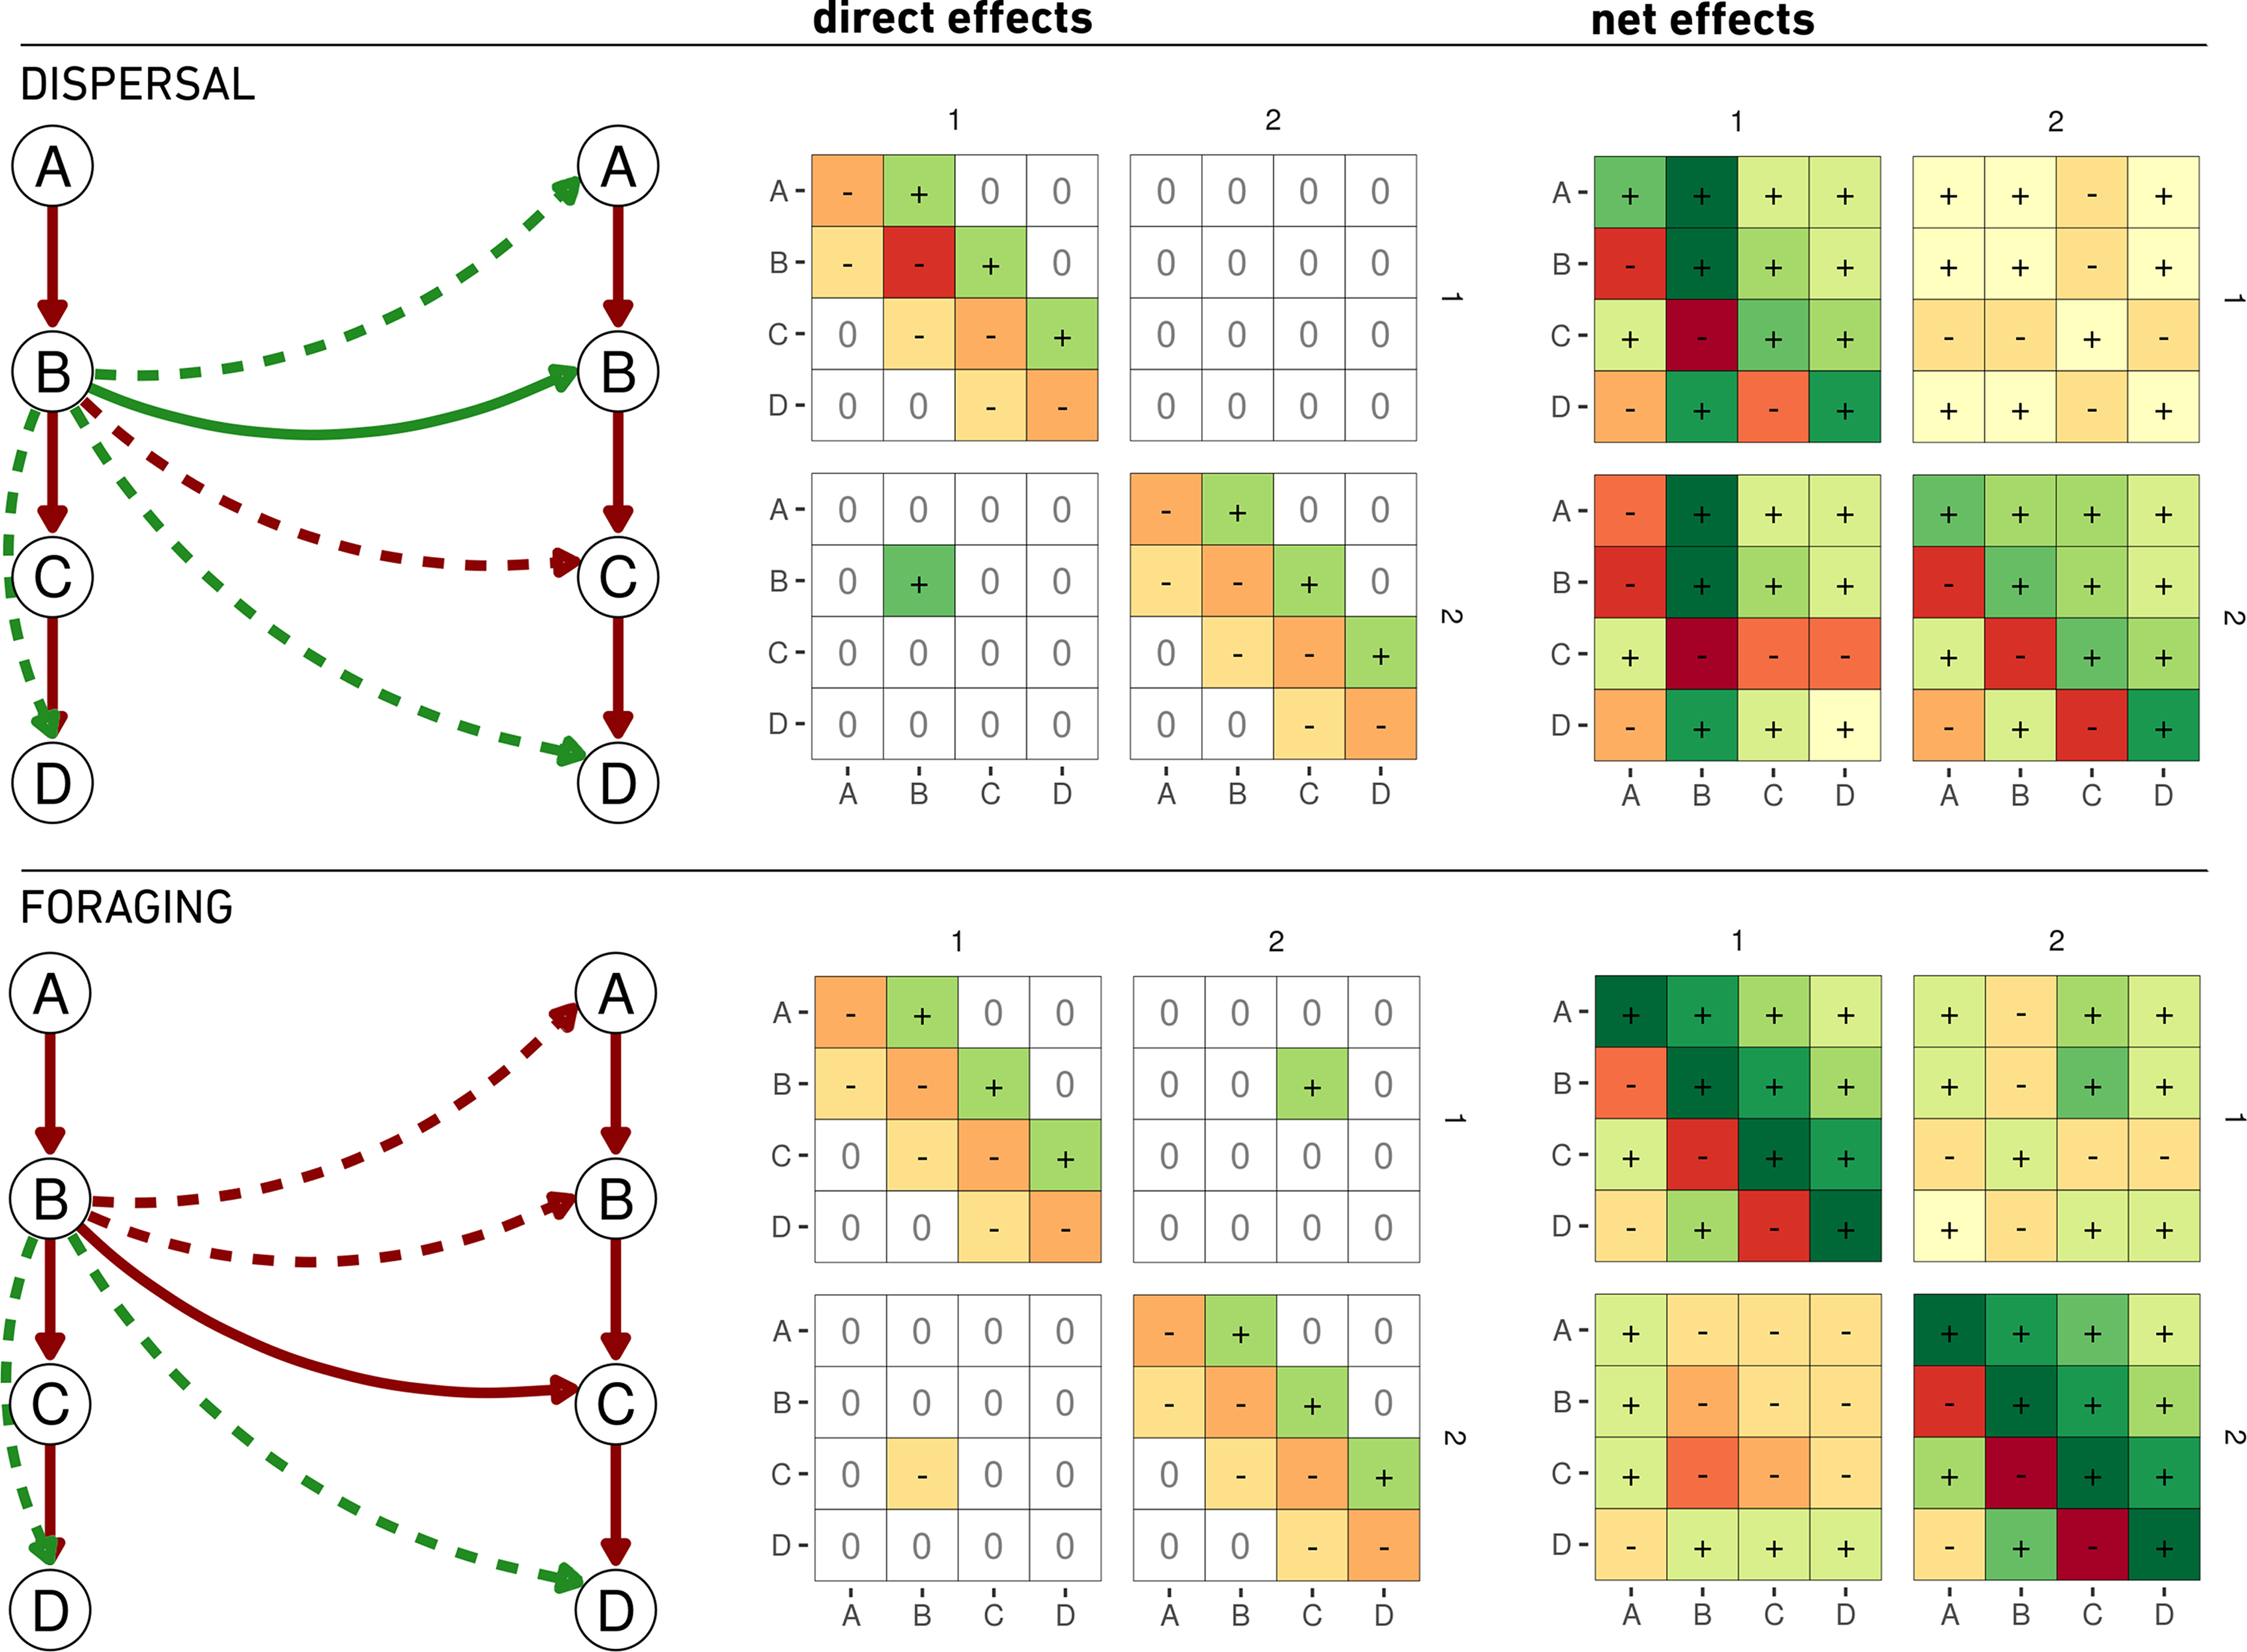
\includegraphics[width=0.95\textwidth,height=\textheight,keepaspectratio]{./Figures/chapter05/Fig_1.png}
\caption[Direct and net effects example]{\color{Gray}Interaction matrices and net effect matrices for two simple configurations. In both cases, a linear food chain is represented at two locations (\textit{1} and \textit{2}). In the dispersal configuration, species B disperses from the first location to the second. In the second configuration, species \textit{B} preys on species \textit{C} on both locations. Green links represent positive effects, red negative. Solid arrows represent direct effects, dashed arrows expected indirect effects. For clarity, in the food chains we display only the indirect effects arising directly from species \textit{B} at location \textit{1}. Darker shades in the matrices indicate stronger effects. The matrices can be read as with the following example: in the foraging configuration, the direct effect of \textit{B} in location \textit{1} over \textit{C} in location \textit{2} is given by locating the column that indicates species \textit{B} at location \textit{1} (the second column of the matrix), and the row indicating species \textit{C} at location \textit{2} (seventh row). }\label{fig:fig5.1}
\end{figure}

Here we study how net effects are propagated in space when local food webs are connected by dispersal, foraging, or a combination of both movement types, using model metacommunities. In particular, we ask the following questions: (1) What is the distribution of signs and magnitudes of net effects in communities connected by dispersal, foraging, or a mixture of both? (2) Are networks of net effects similar in structure to networks of direct effects? (3) Does the magnitude of the net effects between any two species decay with increasing distance between them?

\section{Methods}

We developed a spatially explicit metacommunity model in which local trophic communities are connected through 1) dispersal, 2) foraging, or 3) both. The dynamics of the system are given by a general Lotka-Volterra implementation, following \cite{Gravel2016a}, and for each configuration we ran numerical simulations and recorded both the direct effect and the net effect between each pair of species in the metacommunity, as well as a set of network metrics for characterizing potential differences in metacommunity structure.

\subsection*{Quantification of direct and net effects}
In theoretical analyses of ecological networks, the Jacobian matrix of the system (also called \textit{community matrix}) is widely used to describe the direct effects between each pair of species at equilibrium. In its most common implementation, it represents the effect in one species' growth rate respect to small changes in another species' abundance \citep{Berlow2004, Novak2016}. Consider a general population dynamics model of $S$ species present in $n$ local sites, in which the population density of species $i$ at site $x$ over time is given by

\begin{equation}
\frac{dN_{ix}}{dt} = N_{ix} f_{ix}(N_{1\cdot},...,N_{S\cdot})
\end{equation}

where $N_{ix}$ is the density of species $i$ in site $x$, and $f_{ix}(N_{1\cdot},...,N_{S\cdot})$ its growth rate, potentially influenced by any other species present in any of the $n$ sites (represented by the $\cdot$ notation). In this general case, the elements of the metacommunity Jacobian matrix $C$ are

\begin{equation}
c_{ix,jy} = \frac{\delta (\frac{dN_{ix}^*}{dt})}{\delta N_{jy}^*} = \frac{\delta [N_{ix}^* f_{ix}(N_{1\cdot}^*,...,N_{S\cdot}^*)]}{\delta N_{jy}^*}
\end{equation}

where $N_{ix}^*$ represents the steady state density of species $i$ at site $x$. The net effect of species $j$ at $y$ over species $i$ at $x$, in turn, is the sum of its direct effects and all indirect effects between the two species evaluated at steady state \citep{Bender1984,Montoya2009a,Novak2016}. These can be calculated as the negative of the elements of the inverse Jacobian, i.e. $-(c^{-1})_{ix,jy}$. Specifically, the coefficients $-(c^{-1})_{ix,jy}$ represent the net effect of an increase in species $j$'s population growth rate on the density of species $i$, when all species respond to direct effects \citep{Novak2016}.

\subsection*{The model}

The dynamics of the community are modelled with a general Lotka-Volterra implementation, following \cite{Gravel2016a}. Considering a set of $S$ species present at $n$ locations, the dynamics of species $i$ at location $x$ is given by:

\begin{equation}
\frac{dN_{ix}}{dt} = N_{ix}(m_{ix} + \sum_{y \in n} \sum_{j \in S} b_{ix,jy} N_{jy}) + \Delta N_{ix}
\end{equation}

where $m_{ix}$ is the intrinsic growth rate of species $i$ at location $x$, $N_{ix}$ its abundance, $\Delta N_{ix}$ is the net migration balance, and $b_{ix,jy}$ is the per capita effect of species $j$ at location $y$ on species $i$ at location $x$. This parameter encapsulates the effect of foraging to/from other locations, and it represents a basic situation in which species $i$ forages from its reproductive area $x$ to other locations. Specifically, we assume that a foraging species allocates a fraction $f$ of its foraging efforts to communities outside its reproductive location, which implies that the effort allocated to feeding in its local community is $1-f$. We incorporate this in our model as follows:

\begin{equation}
b_{ix,jy} =
\begin{dcases*}
   (1-f)\alpha_{ix,jy}        		& if $x = y$ \\
   \frac{f}{\vert n_{ix} \vert}\alpha_{ix,jy}     & if $x \neq y, \alpha_{ix,jy} > 0$ \\
   \frac{f}{\vert n_{jy} \vert} \alpha_{ix,jy}    & otherwise
\end{dcases*}
\end{equation}

The first situation corresponds to the effect of predation from the same location, in which case the interspecific interaction coefficient $\alpha_{ix,jy}$ is weighted by the relative effort dedicated to foraging within its home location ($1-f$). The second situation represents foraging of species $i$ at location $x$ on species $j$ at location $y$. The net foraging effort $f$ is equally divided among all locations reachable by species $i$ from location $x$ (the set given by $n_{ix}$, which has a cardinality of $\vert n_{ix} \vert$). The last situation is the opposite, where species $i$ at location $x$ is preyed upon by species $j$ at location $y$. In this case, $f$ is divided among all locations reachable by species $j$ from location $y$. Note that this situation represents an equal division of foraging effort among all reachable locations.

Dispersal among different locations, in turn, is represented simply by the net variation in species densities between reachable locations, modelled by passive diffusion with dispersal coefficient $d$ \citep{Gravel2016a}:

\begin{equation}
\Delta N_{ix} = \sum_{y \in n_{ix}} \frac{d_{ixy}}{\vert n_{ix} \vert} (N_{ix} - N_{iy})
\end{equation}

Thus, as it is the case with foraging, dispersal effort $d$ is divided equally among all patches reachable by species $i$ on location $x$.

\subsection*{Parameterization and simulations}

We considered predator-prey interactions, but the approach could easily be generalized to other types of interactions. The structure of local communities, i.e. who interacts with whom, is determined according to the niche model \citep{Williams2000}, ensuring that there were no disconnected species. We further assumed that the niche axis obtained from the niche model is linearly correlated with the foraging and dispersal distance of the different species, such that the species with lowest niche values could only forage or disperse to adjacent communities. Interaction coefficients $\alpha$ at the regional scale are drawn from a normal distribution $N(0.25,0.1)$, with the sign structure given by the niche assembly model. We introduced a small amount of spatial heterogeneity by drawing local coefficients from a normal deviate with mean centered on the corresponding regional coefficients and standard deviation of 0.1.

Local communities were placed along a single dimension space, which ends were connected together in order to (1) maximize potential path lengths between non-connected communities, and (2) prevent edge effects of communities at the end of the linear chain. We fixed the maximum dispersal and foraging distances to two cells away from the species' home location in order to avoid excessive parameterization and for better comparing the net effects of the different movement types.

With this setting, we simulated the dynamics of 15 species at 10 local communities. The number of species and size of the landscape correspond to a meta-adjacency matrix of $15*10 = 150$ rows. This size was chosen in order for the numerical calculation of the Jacobian matrices to be computationally feasible. Although a relatively small species richness and number of patches, it is sufficient to explore spatial distances and patch lengths of over 5 units.

We generated three sets of simulations: only dispersal, in which we set the dispersal coefficient $d = 0.5$, and the foraging coefficient $f = 0$ for every species; only foraging, with $d = 0$ and $f = 0.5$; and dispersal and foraging, with $d = 0.5$ and $f = 0.5$.

We run 100 random topologies from each configuration, and for each replicate we obtained numerically the direct and net interaction coefficients between each pair of populations in the metacommunity, which could then be (1) qualitatively compared and (2) analyzed with regards to the distance between the interacting populations. We also computed basic quantitative descriptors of the direct and net effects networks at equlibrium: the \textit{connectance} of the metacommunity networks; their \textit{average path length}, i.e. the average of the shortest path lengths between any pair of populations in the metacommunity; and their \textit{modularity}, which measures the tendency for nodes to be grouped into distinct modules \citep{Newman2006}. Here, we calculate a weighted version of modularity that considers both positive and negative link weights, as implemented in the R \textit{igraph} package \citep{Csardi2006}.

\section{Results}

\subsection*{What is the distribution of signs and magnitudes of net effects in communities connected by dispersal, foraging, or a mixture of both?}

Net effects (i.e. elements $-(c^{-1})_{ix,jy}$ described above) are mainly of equal sign as direct effects (i.e. elements $c_{ix,jy}$ of the Jacobian matrix) when local communities are connected by dispersal (Table \ref{tab:tab5.1}), whereas in foraging and mixed modes of movement, sign switches occur in around 50\% of pairwise interactions. In all simulations, however, the ratio of positive to negative net effects is maintained at values close to 1, meaning a similar number of positive and negative net effects for all configurations.

\begin{table}[h]
\centering
\caption[Spatial effects summary metrics]{\color{Gray} Summary metrics of the simulations performed. For each simulation, we group the results by location, i.e. whether the interaction occurs between species of the same (intra-) or different (inter-) patch. We show the ratio of positive to negative net effects, and the relative frequency of pairwise interactions that switch sign from direct to net effect.}\label{tab:tab5.1}
\begin{tabular}{lllll}
\hline
movement mode          & location & +/- ratio & \multicolumn{2}{l}{sign switches} \\
\cline{4-5}

                       &          &           & + to -          & - to +          \\
\hline
dispersal              & intra-patch   & 0.95      & 0.07            & 0.33            \\
					  & inter-patch   & 1.03      & 0.002           & 0               \\

\hline
foraging               & intra-patch   & 1.02      & 0.51            & 0.47            \\
                       & inter-patch   & 0.97      & 0.42            & 0.41            \\

\hline
dispersal and foraging & intra-patch   & 1.02      & 0.52            & 0.57 \\
                       & inter-patch   & 1.02      & 0.48            & 0.49            \\

\end{tabular}

\end{table}

The three modes of movement displayed distinctly different net effects signatures on interactions occurring both within the same location (intra-patch) and across different locations (inter-patch) (Fig. \ref{fig:fig5.2}). Intraspecific effects are generally positive across locations in the dispersal configuration, and also positive in the local food webs (upper panel of Fig. \ref{fig:fig5.2}). This trend is blurred for foraging and mixed movement modes, where intraspecific effects are more variable and have a higher frequency of negative magnitudes (Fig. \ref{fig:fig5.2} middle and lower panels). Net effects are also generally of the same sign in local patches and across patches when communities are connected by dispersal (orange points on the upper panel of Fig. \ref{fig:fig5.2}). Again, this trend is diluted when foraging is accounted for, in which case intra-patch and inter-patch net effects display any combination of positive and negative signs, with no clear trend. Although here we analyze the results for $d = 0.5$ and $f = 0.5$, the distinctiveness of the dispersal and foraging patterns is maintained across a range of $d$ and $f$ values (Appendix 5.1).

\begin{figure}[!ht]
\centering
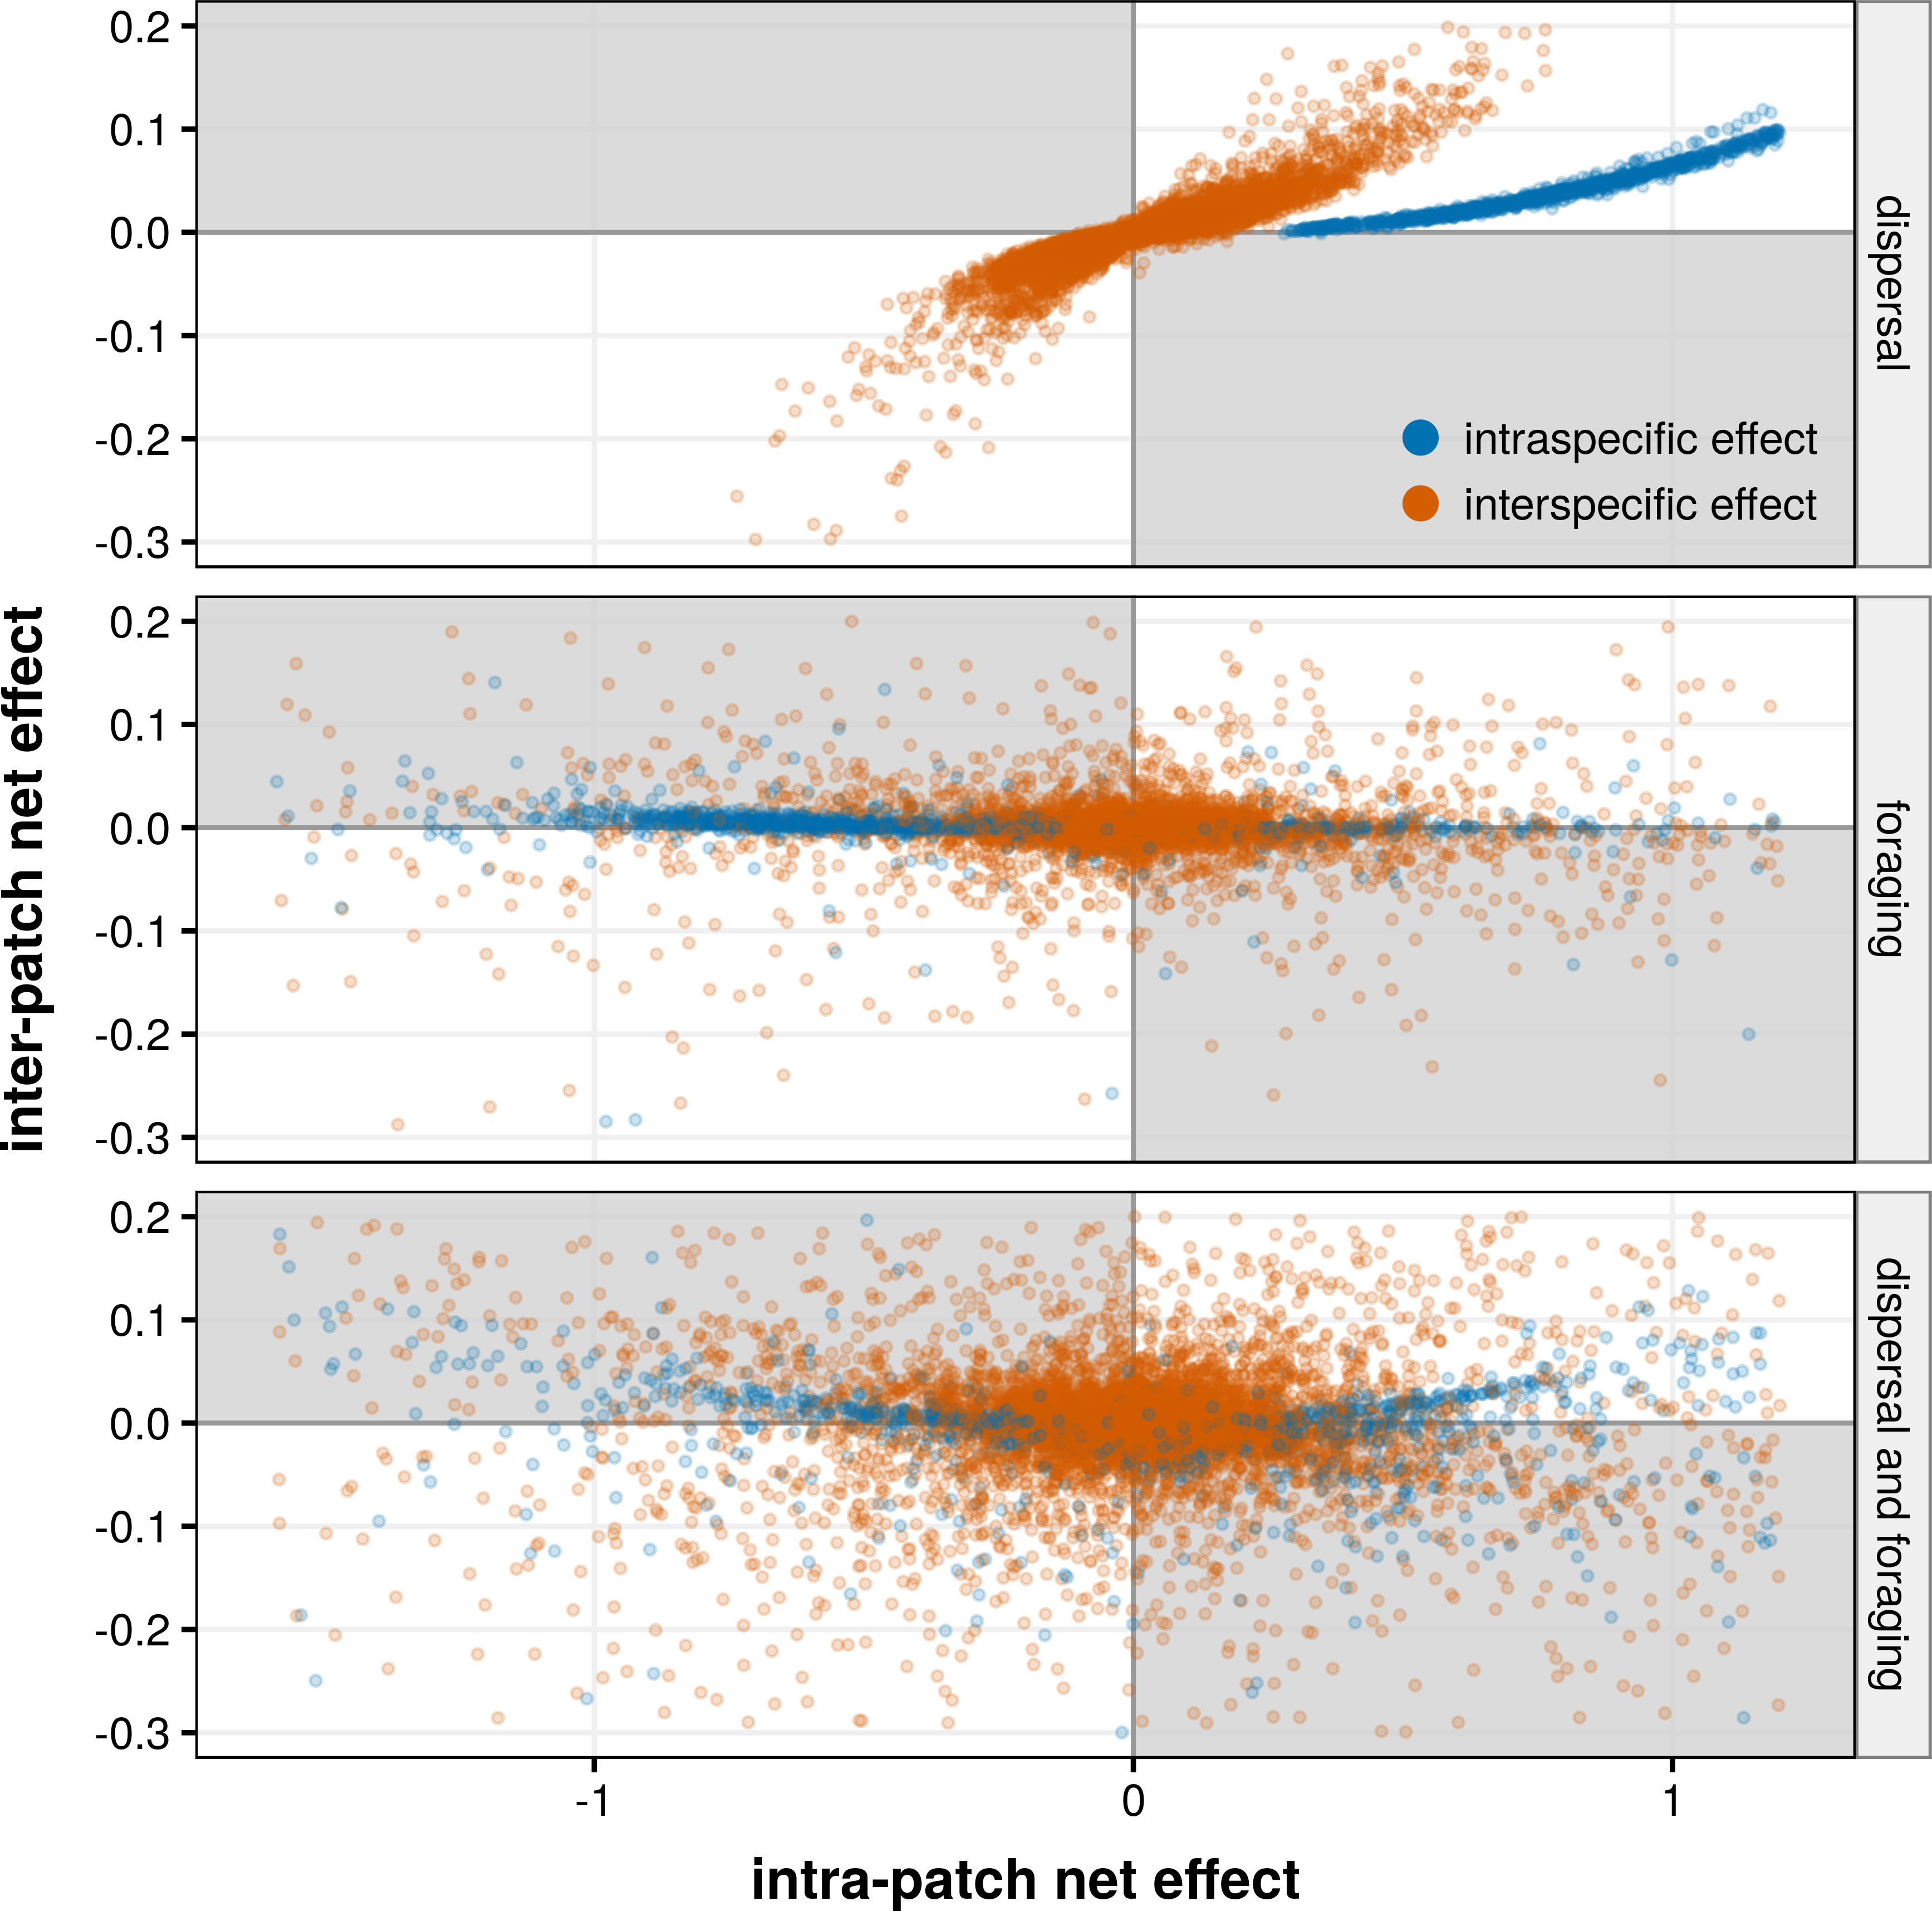
\includegraphics[width=.7\textwidth,height=\textheight,keepaspectratio]{./Figures/chapter05/Fig_2.png}
\caption[Intra and interpatch net effects]{\color{Gray}Distribution of intra and inter-patch net effects in the three configurations. Shaded quadrants are those where a sign switch occur between intra and inter-patch effects.}\label{fig:fig5.2}
\end{figure}

\FloatBarrier

\subsection*{Are networks of net effects similar in structure to networks of direct effects?}

There exist non-zero net effects between virtually every species in the model metacommunities, as expressed by net effect networks having connectances and path lengths of 1 in all cases (Fig. \ref{fig:fig5.3}). In contrast, direct effect networks are obviously not fully connected, displaying intra-patch connectances at steady state of 0.38 on average and inter-patch connectances between 0.01 (dispersal only) and 0.1 (dispersal and foraging). Weighted modularity is also much higher in the direct effects networks than in the net effects ones, as expected. However, the modularity of the net effects networks also shows a decreasing trend from dispersal only networks to dispersal and foraging ones (Fig. \ref{fig:fig5.3}).

\begin{figure}[ht]
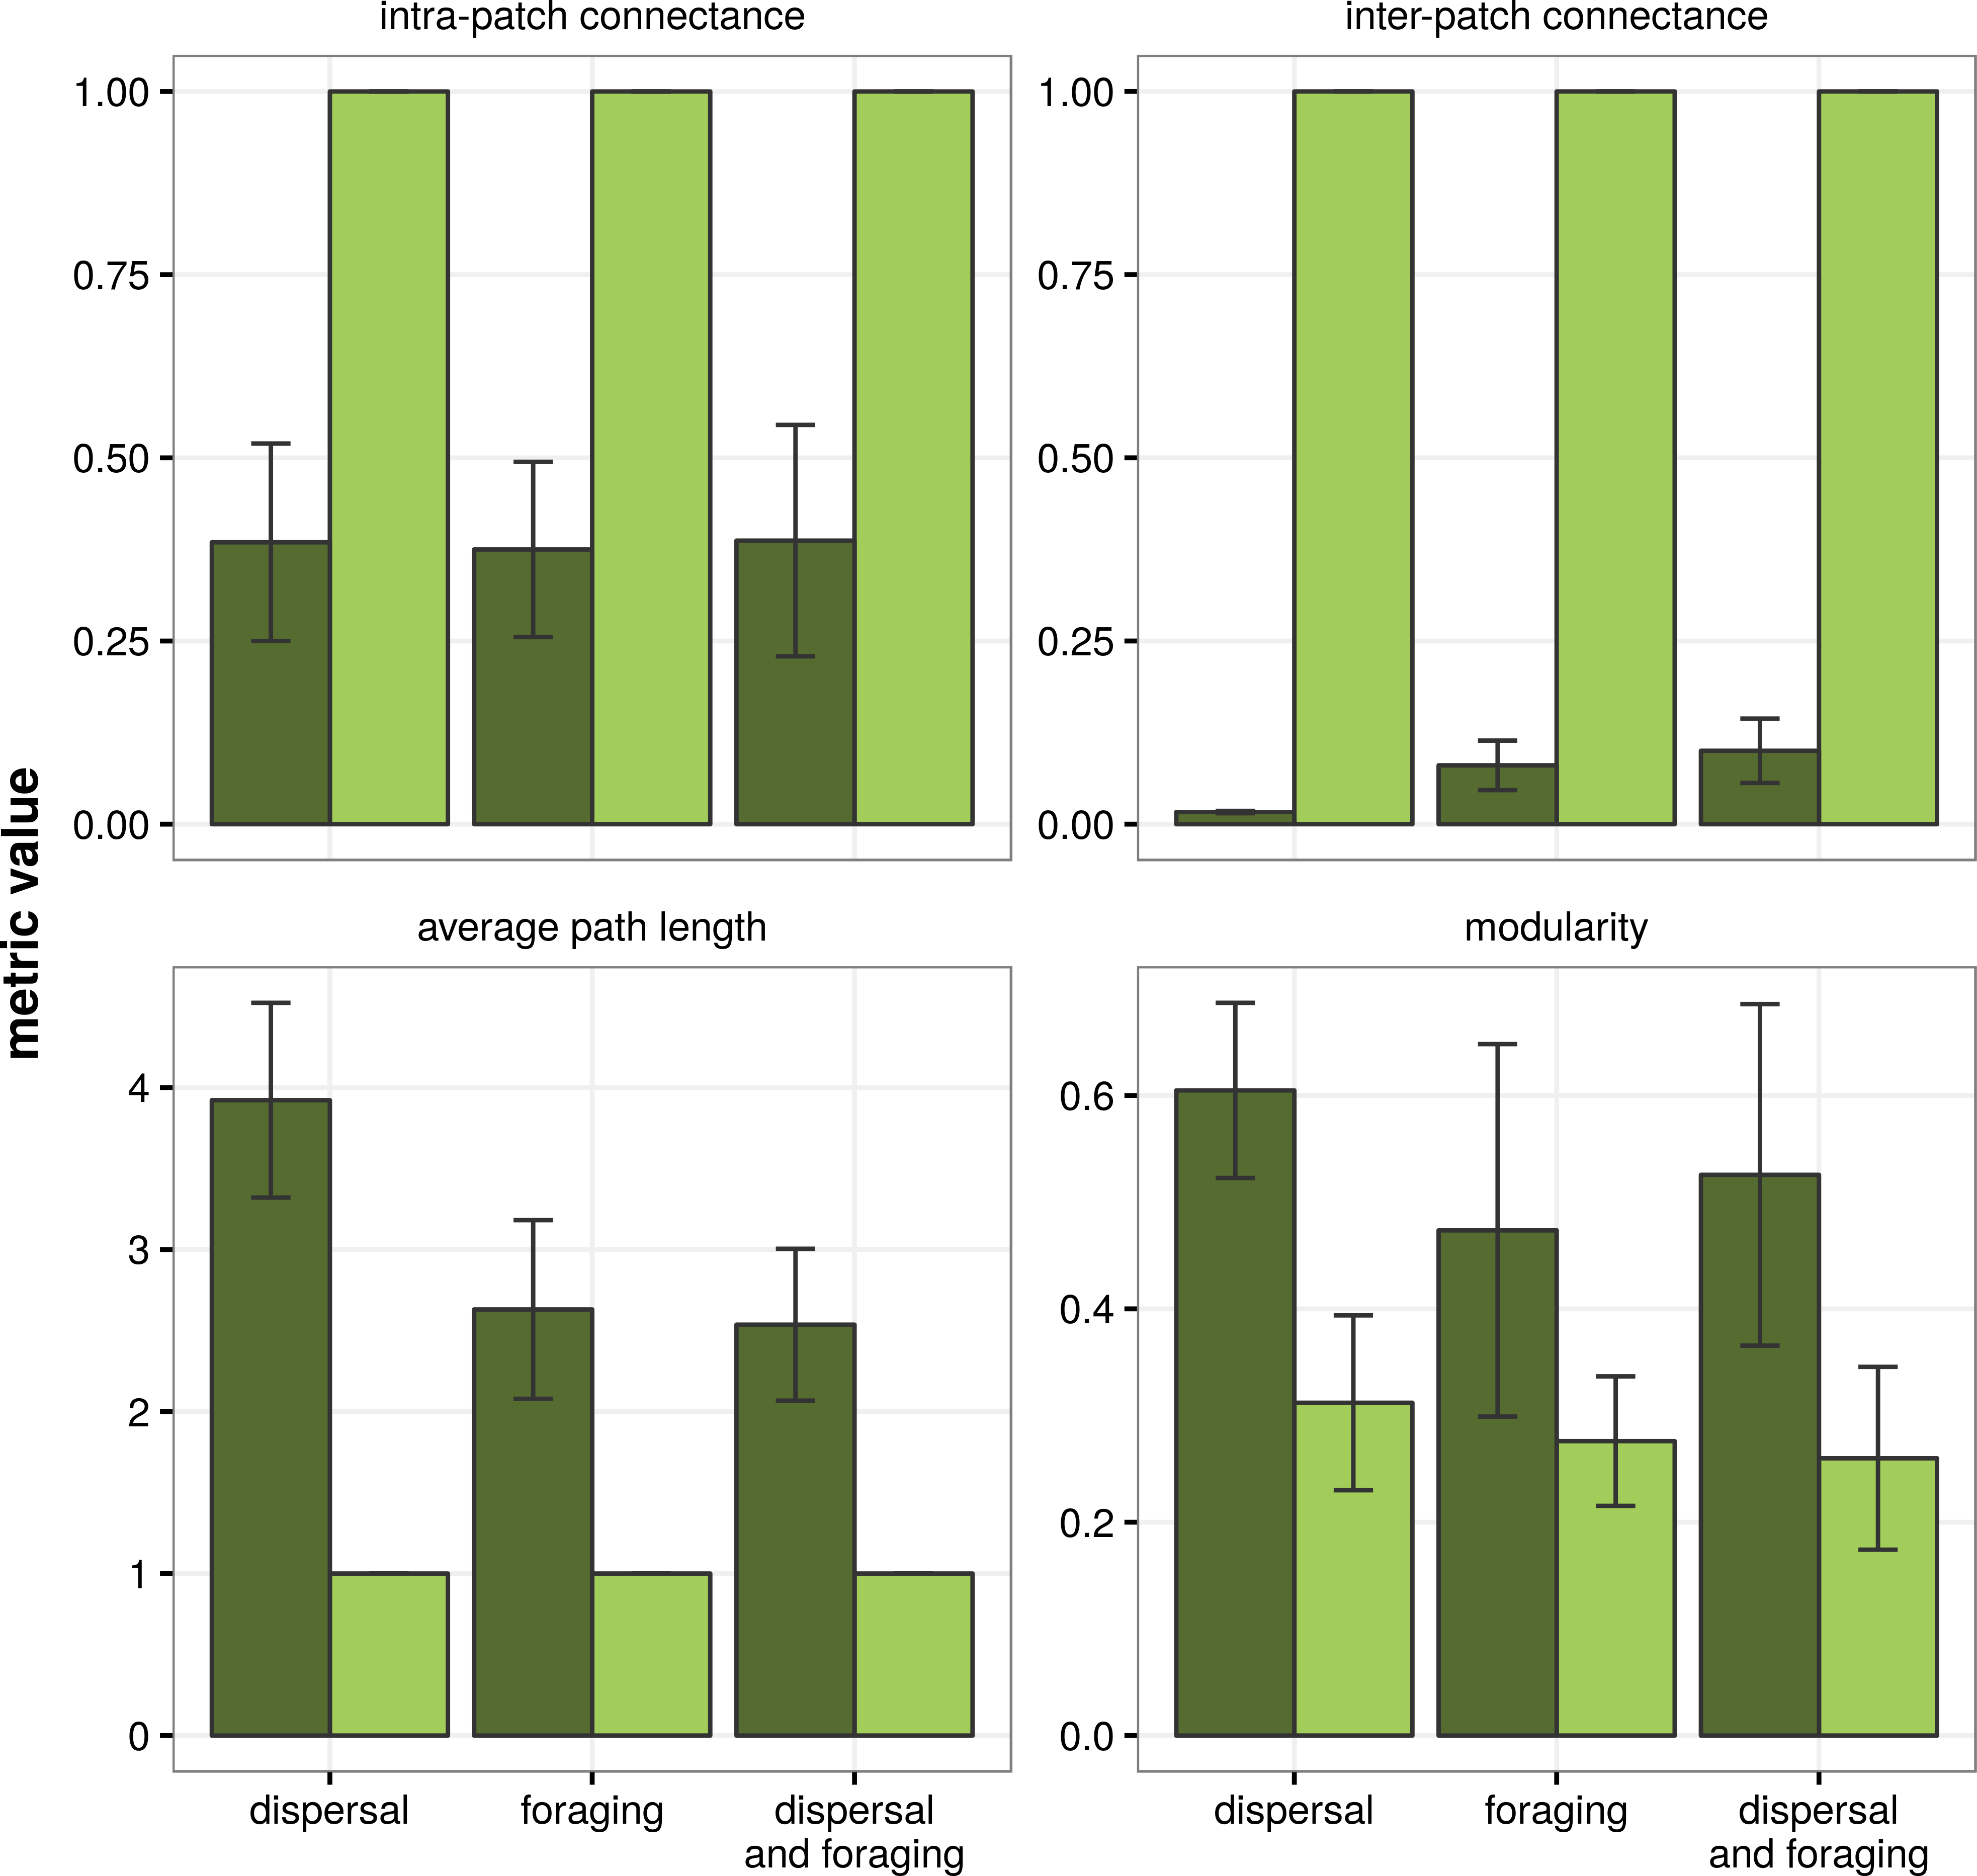
\includegraphics[width=.7\textwidth,height=\textheight,keepaspectratio]{./Figures/chapter05/Fig_3.png}
\centering
\caption[Metacommunity network metrics]{\color{Gray}Network metrics of the metacommunities at equilibrium. Dark shades represent networks of direct effects, light shades networks of net effects.}\label{fig:fig5.3}
\end{figure}

\FloatBarrier

\subsection*{Does the magnitude of the net effects between any two species decay with increasing distance between them?}

The magnitude of spatial cascades is influenced by the length of its associated food chain. Net effects between any pair of species decrease in magnitude with the spatial distance between the two species (i.e. the distance between their home locations, assuming that connected locations are at distance $1$ from each other). This decrease is even sharper when the distance metric considered is the path length between the two species, i.e. the number of connections separating them (Fig. \ref{fig:fig5.4}). This result is observed in the three movement modes, although the decay rate is generally highest for foraging configurations. The trend is also robust to variations on dispersal and foraging rates (Appendix 5.1).

\begin{figure}[ht]
\centering
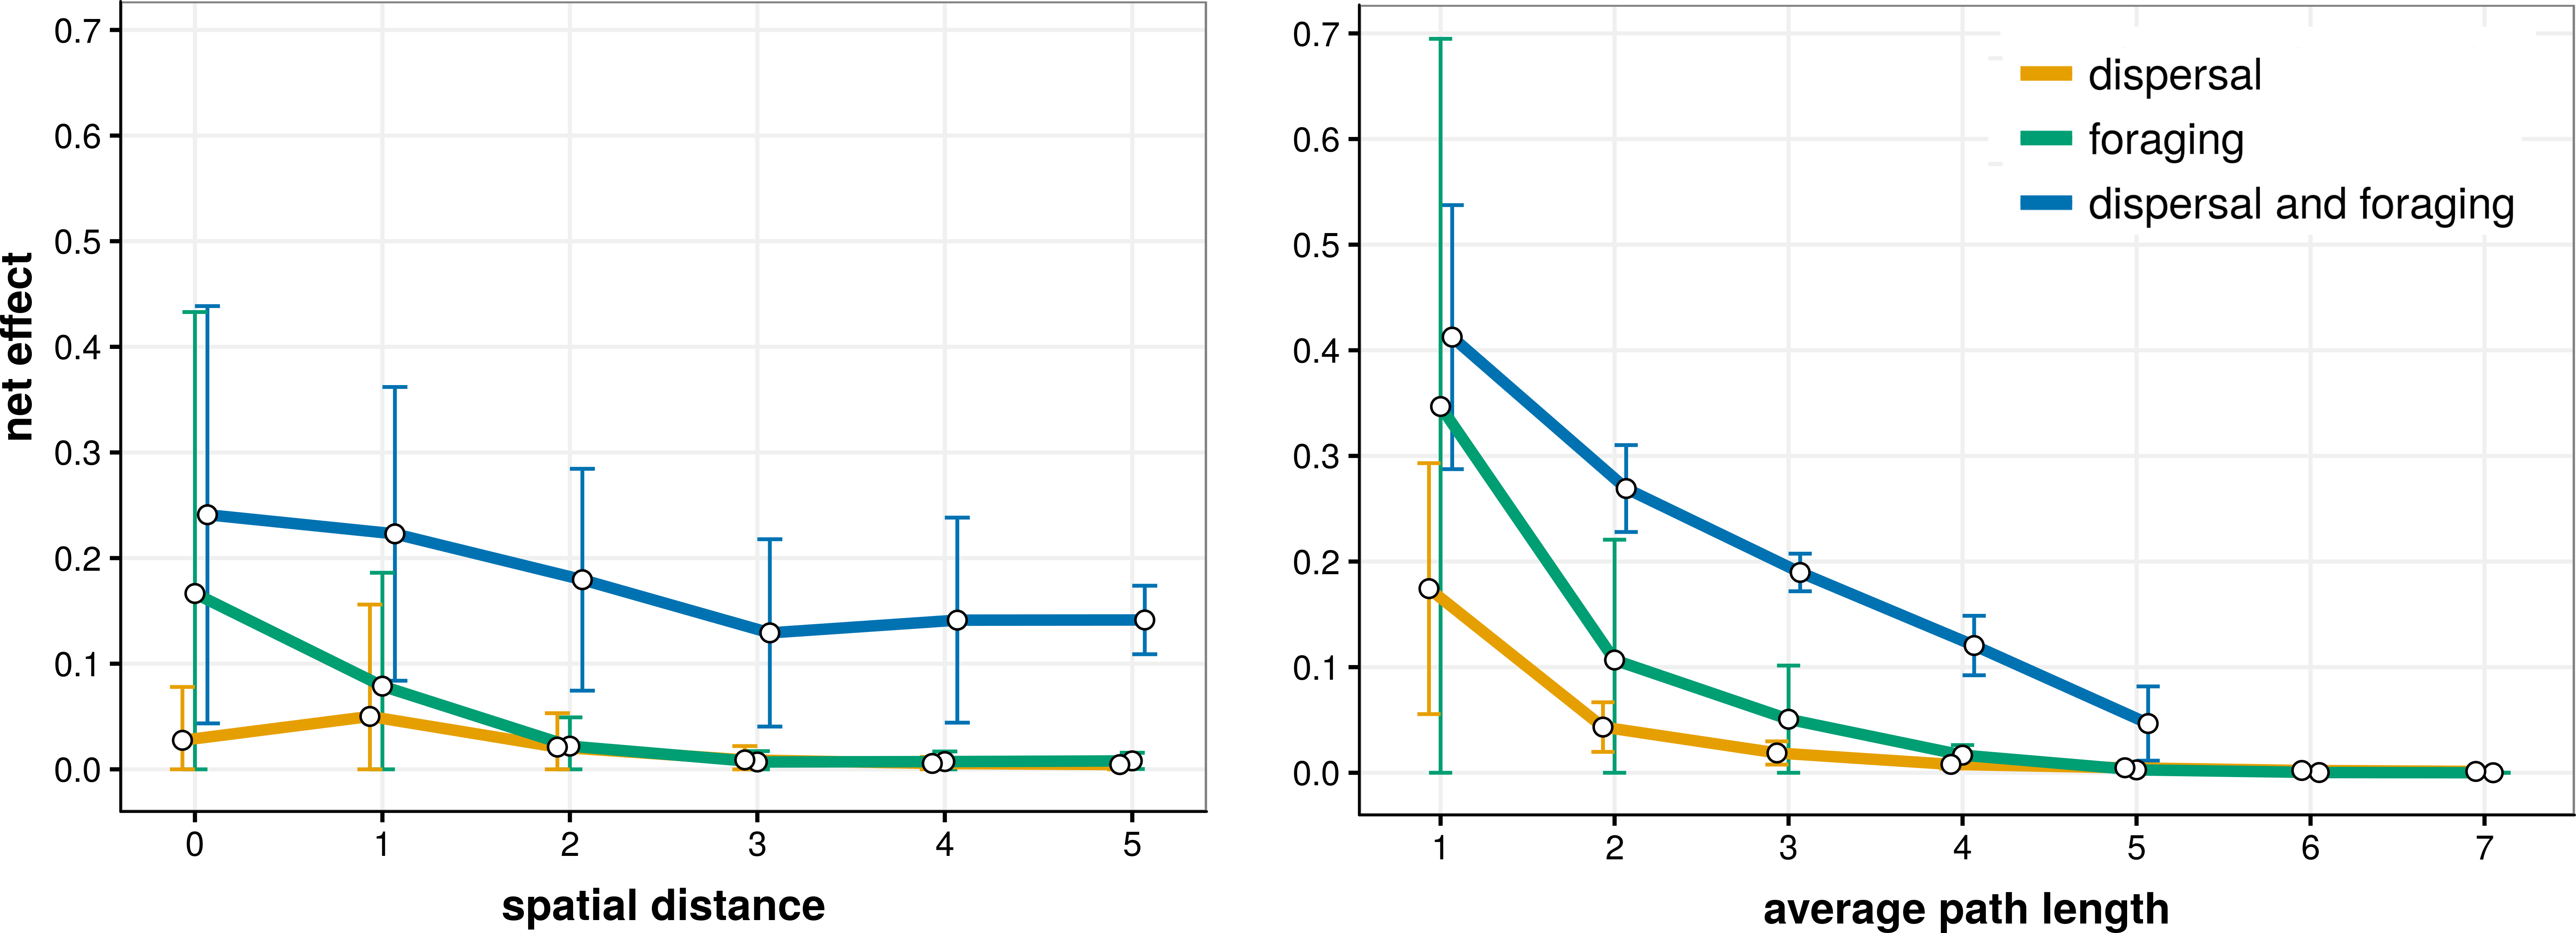
\includegraphics[width=.9\textwidth,height=\textheight,keepaspectratio]{./Figures/chapter05/Fig_4.png}
\caption[Spatial decay of interaction effects]{\color{Gray}Net effect between species pairs as a function of \textit{a)} spatial distance between patches, \textit{b)} average path length between species. Values are averaged over all replicates, and error bars represent averages +/- one standard deviation.}\label{fig:fig5.4}
\end{figure}

\FloatBarrier

\section{Discussion}

The importance of indirect effects, including trophic cascades, in driving ecosystem dynamics and structure is well established in theory \citep{Abrams1992, Wootton2002, Gravel2010, Mayfield2017} and on the field \citep{Menge1995, Peacor1997, Moya-Larano2007, Barbosa2017, Trussell2017}. The propagation of these effects across space has however not been studied systematically, despite many scattered observations of spatially explicit trophic cascades \citep{Polis1997, Estes1998, Knight2005, Casini2012, Springer2018}. Here we lay down basic tenets on how interaction effects are propagated in space depending on whether species connect different local communities via dispersal, foraging, or both modes of movement. We show that model metacommunities with populations connected by dispersal and foraging differ on (1) the proportion of pairwise interactions that switch sign between their direct and net effects, and (2) the sign and magnitudes of net effects on the local patch and across patches. Furthermore, the networks of net effects are markedly different from the direct effect ones, in all cases. Last, we observed that, in most cases, the magnitude of net effects between any two populations decays significantly with the distance between the two populations. In particular, the strongest decay occurs when distance is measured as the number of spatial connections necesary for linking the two populations.

Indirect effects may generate unexpected net interaction outcomes between pairs of species. For example, \cite{Montoya2009a} analyzed a set of well-resolved empirical food webs and showed that the influence of indirect effects induced a switch in interaction signs from direct to net effect for approximately 40\% of species pairs. Using a similar approach, we show that net effects between populations of spatially disconnected communities may also be primarily driven by indirect feedbacks, as for example, cases in which a species foraging on a secondary location indirectly benefits its prey on this second location by altering the dynamics of the whole food web. This theoretical possibility has, to our knowledge, not been tested in empirical systems.

The ``signatures'' of net effects produced by dispersal, foraging, or mixed modes of movement across localities are clearly different from each other \citep{Amarasekare2008} even though we imposed equal maximum dispersal and foraging distances, and after accounting for different values of dispersal and foraging rates (Appendix 5.1). In the dispersal scenario, the almost complete concordance between the sign of intra- and inter-patch net effects points to a relatively homogeneous role of species at local and regional scales. Therefore, in natural systems with the same species pool connected mainly by dispersal, a local evaluation of the influence of the dispersing species may offer insights for the whole metacommunity. In the foraging or mixed modes, however, interspecific net effects derived from the populations of the same and different locations often switch signs, without showing any clear trend (middle and lower panels of Fig. \ref{fig:fig5.2}). Therefore, within the assumptions of our model, when foraging is a prevalent mode of movement across locations, interspecific effects between any two species cannot be extrapolated from the local to the regional scale. In other words, a consumer that decreases a prey locally may have a positive effect on the same prey at the regional scale. Note, however, that our baseline scenario represents communities within an homogeneous habitat, the same species pool in all locations, with no density-dependent movement modes, no active selection or other types of heterogeneity. Furthermore, we deliberately chose dispersal and foraging modes of movement with identical maximum distances and temporal dynamics, in order to highlight their intrinsic differences. In reality, of course, both dispersal and foraging have extremely variable spatiotemporal scales. Foraging, in general, happens much faster than local demographic dynamics, which has led to characterize its effects as \textit{spatial coupling} of local communities \citep{Massol2011}. This spatial coupling is thought to dampen population oscillations at lower trophic levels \citep{McCann2005}. The effects of dispersal, on the other hand, occur on temporal scales comparable to those of local dynamics, favouring different types of coexistence relationships, such as source-sink dynamics. The relative scales of foraging and dispersal are very heterogeneous, so that the spatial signal of interaction cascades will likely be correlated, in general, with these movement-related traits. In our model, we restricted the maximum dispersal and foraging rates to two cells away from the local community, and different values will presumably alter the net effect decay with spatial distance (Fig.  \ref{fig:fig5.3} left panel). Interestingly, the decay of net effects with path length (Fig.  \ref{fig:fig5.3}, right panel) did not vary strongly with increases in maximum movement rates in our model ($d$ and $f$, see Appendix 5.1). This result suggests that indirect effects may dampen the propagation of strong interactions across space, at least in environments with similar habitats and species pools.

Networks of net effects are fully connected (Fig. \ref{fig:fig5.3}), meaning that every species has a non-zero influence in every other species of the metacommunity, through direct and/or indirect pathways. The number of connections between local communities increases from dispersal to foraging modes, and is maximal when both modes are combined. This is reflected in the weighted modularity of the net effects networks, which tends to decrease along that axis. In the simple metacommunities modelled here, these structural patterns of the net effect networks are mostly confirmatory, but such analyses, when feasible, should provide novel insights into the structure and dynamics of more complex communities and metacommunities.

Dispersal generally represents unidirectional organismal movement across localities, with no associated direct movement of material. Foraging, on the other hand, involves a processing of organic material from the foraged location to the home location \citep{Gounand2018}. This two-way coupling has consequences for the role of the different locations as demographic sources or sinks \citep{Gravel2010}. In general, although here we have focused on movements of organisms across localities, the physical transfer of material often plays a key role in the structure and dynamics of the local communities \citep{Polis1997}. For example, the nutrients accumulated by Pacific salmon in open waters are transported to freshwaters during the spawning season, indirectly affecting terrestrial plants and animal populations \citep{Naiman2002, Levi2012}. The integration of these \textit{ecological subsidies} with organismal movement is well develeoped theoretically in the framework of metaecosystem theory \citep{Loreau2003, Gounand2018}. We have provided a first approach to the explicit modelling of foraging behaviours in metacommunities, but its coupling with material transfers will expand and refine the results presented here. In a related question, most empirical studies on ecological subsidies are focused on transfers between different habitats, which usually involve specialized interactions (e.g. the consumption of Pacific salmon by grizzly bears) or species with life stages in different habitats, such as arthropods with aquatic larval stages that, in their adult form, switch to a predator role in terrestrial habitats. We, in turn, modelled communities with a small amount of spatial heterogeneity but the same pool of species and interactions on each patch. It is likely that interactions connecting different habitats are more specialized and have greater indirect effects than the general foraging interactions modelled here (in what has been called \textit{keystone interactions}, \citealt{Helfield2006}). This specificity is likely to alter both the structure of the overall meta-network (Fig. \ref{fig:fig5.3}) and the distance decay curves observed in our model system (Fig. \ref{fig:fig5.4}). For example, \cite{Knight2005} showed how predatory fish could have strong net effects on terrestrial plants through a series of specialized interactions, even though the number of links separating these species is four (fish-dragonfly larvae-dragonfly adults-insect pollinators-plants).

Spatial patterns of net effects can also vary from our baseline expectations depending on the distances covered by the foraging or dispersing species. Intercontinental migrations are an extreme example of this, where strong coupled effects occur between species separated by thousands of kilometers \citep{Alerstam2018}. Further, such migratory movements connect localities at different moments in time, rather than continuously. The effect of such temporal decoupling may provoke strong oscillatory dynamics between systems \citep{Springer2018}, although in general, the stability dynamics associated with migrations have received little attention to date. Overall, the interplay between the rates and distances of dispersal and foraging, and their relationship to the spatial decay of net effects, clearly needs more attention in theoretical models and empirical studies. For example, experimental mesocosms allowing spatial movement of certain species among them may be used to test the differential influence of foraging and dispersal on local dynamics.

\section{Conclusions}

We have provided a theoretical basis to the study of spatial propagation of indirect effects across ecosystems. We have shown that the net effect patterns generated by dispersal and foraging movements are clearly different. Furthermore, the structure of the metacommunity networks is markedly different depending on whether one considers direct interactions or net effects between species. The decay of net effect magnitude with distance, in our model, is the only result common to all simulations performed. These results may shed light on the spread of interaction effects in patches of the same habitat type, such as forest patches inserted in agricultural or urban areas. Furthermore, they represent a baseline case for developing more complex scenarios, such as the effects of interaction spread (1) across different habitat types and species pools, or (2) when material fluxes are accounted for.

%%************************************************
\chapter[Interactions and environmental factors]{Community responses to resource and non-resource environmental gradients}\label{ch:environment}
%************************************************
\tikz[remember picture,overlay] \node[opacity=0.3,inner sep=0pt] at (current page.center){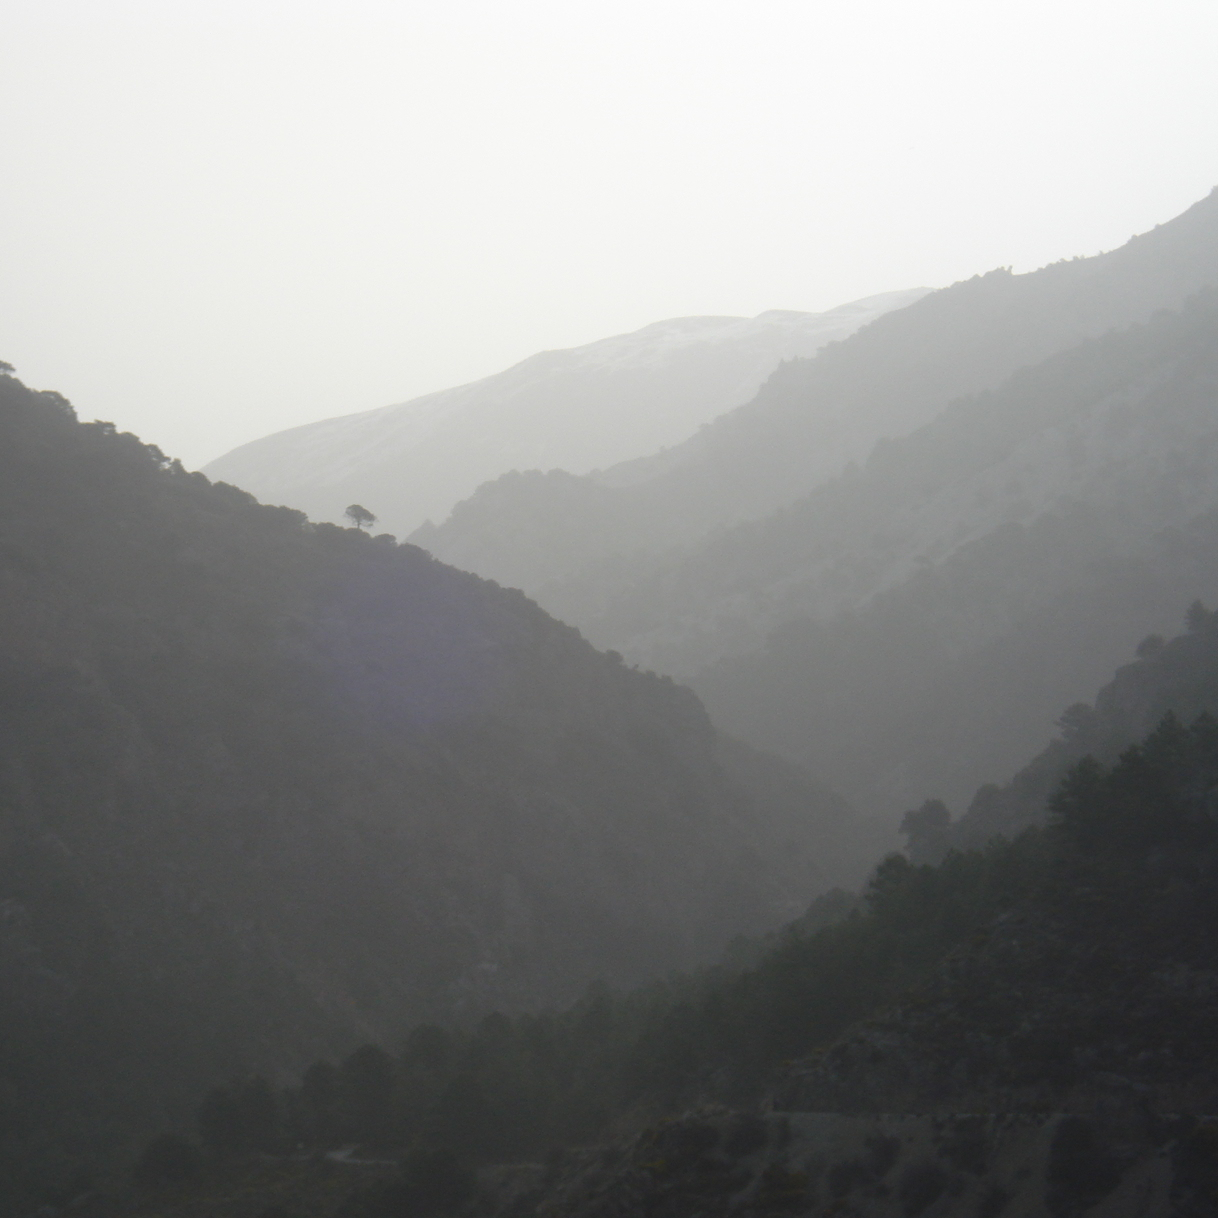
\includegraphics[width=\paperwidth,height=\paperheight]{./Figures/cover/granada_2_pagina.jpg}};
\clearpage

\section*{Abstract}

Environmental variations are a driving force behind virtually all ecological patterns. Different types of environmental gradients are bound to trigger differential responses at the species and community level, but this variability among environmental factors has been largely overlooked in current community ecology paradigms. We argue that the distinction between resource and non-resource factors, originally proposed by Evelyn G. Hutchinson, provides a convenient way to classify environmental factors, as these two types have different effects on ecological interactions and emergent community properties. Using a community model with environmental variability on a resource and a non-resource factor, we show that the intensity of competitive interactions is driven jointly by variations in both gradients, whereas facilitation intensity is driven solely by the non-resource factor. Likewise, species richness and persistence times of species are mainly driven by variations in the non-resource factor. These results, derived for simple model communities, suggest the possibility that these two broad types of environmental gradients trigger different bottom-up and top-down feedbacks in more complex communities.

\section{Introduction}

Understanding how environmental factors influence ecological processes is one of the main goals of ecology, and is becoming increasingly relevant in the context of the ongoing global change \citep{Vitousek1994}. Environmental factors influence directly or indirectly virtually every biological process on Earth, and can be extremely varied in their physical characteristics, magnitude, spatial and temporal scale. Furthermore, individuals may interact and respond to their physical environment in very different ways: sessile primary producers acquire inorganic nutrients from their surrounding environment and can often modify their local microclimate, whereas animals are able to move or alter their behaviour in response to environmental variations. Despite the enormous variability in environmental variables and species responses, different environmental factors are commonly lumped together when studying ecological processes across observed gradients, in what are termed “(environmental) stress gradients” (e.g. \citealt{Hart2013}).

As a consequence of this common simplification of environmental factors, there is no overarching theory predicting how different facets of the environment will influence ecological processes at different levels of organization. Developing, or as we will suggest here, recovering a simple but comprehensive “taxonomy” of environmental factors is a key step towards such a theory. To our knowledge, only a handful of studies have attempted to derive a systematic characterization of environmental factors. For example, \cite{Menge1987} made the distinction between physical and physiological stress types, that differ on whether low values of the factor at hand influence survival. Although their classification is readily applicable to any species and gradient, it is not informative about which factors may drive variations in pairwise interactions or resource consumption, which are key processes for maintaining species coexistence.

In the context of niche theory, Evelyn G. \cite{Hutchinson1978} proposed the distinction between scenopoetic and bionomic variables that shape the n-dimensional environmental niche of a given species. Scenopoetic variables are, literally, “scene-setting” factors, abiotic conditions that cannot be consumed, whereas bionomic variables are those consumed by the species or guild in question, thus altering their local dynamics. This distinction has been acknowledged, with a different terminology, in studies of vegetation composition across gradients \citep{Austin1990}. In addition, the stress gradient hypothesis, in its general form, posits that variations in stress levels will drive variations in the intensity of competitive and facilitative interactions among primary producers, with positive interactions becoming more prevalent under harsh conditions \citep{Bertness1994}. A few studies have explored how this hypothesis might be improved by distinguishing resource (i.e. bionomic) and non-resource (scenopoetic) environmental factors. For example, a recent study suggested varying outcomes of pairwise interactions under gradients of different types of factors \citep{Maestre2009}, whereas a compilation of empirical data showed similar shifts towards facilitative interactions across gradients of different stress types \citep{He2013}. Despite these recent developments, most empirical tests of the stress gradient hypothesis do not explicitly consider the implications of studying resource, non-resource, or combined gradients. Furthermore, this diversity of factors has thus far been left out of other influential frameworks in community ecology, such as Tilman’s resource ratio theory \citep{Tilman1980, Miller2005}, environmental stress models \citep{Menge1987}, or Chesson’s coexistence theory \citep{Chesson2000}.

We propose to reintegrate the fundamental distinction between environmental factors coined by \cite{Hutchinson1978} into current ecological paradigms. Hutchinson’s categorisation provides a simple dichotomy for environmental factor types that is relevant for evaluating physiological responses, and most importantly, the outcome of direct pairwise interactions and other community-level responses to environmental gradients. Maintaining the terminology that has recently been developed under the umbrella of the stress gradient theory, we propose to keep the name of resource and non-resource environmental factors for bionomic and scenopoetic variables respectively (Fig. \ref{fig:fig6.1}).

While at the individual level most species will display varying physiological response curves for specific factors regardless of their resource or non-resource quality, the distinction between these categories becomes important when looking at the differences of these response curves between species. As such, we may expect responses to resource factors to be nested for groups of species, while responses to non-resource factors will likely tend to have different optima for different species of a guild \citep{Austin1990}.

Looking at community-level responses, we hypothesize that variation in resource factors will directly drive exploitative competition within species of the same trophic guild, whereas variation in non-resource factors will, instead, drive changes in the intensity and importance of facilitation, and only indirectly will affect competition. These pairwise effects will, in turn, drive different outcomes for species persistence or diversity, among other properties, across different types of gradients.

Here we test these hypotheses using a community model in which we incorporate gradients of resource and non-resource environmental factors. In particular, we ask: (1) does the intensity of competitive and facilitative interactions vary across a combined resource and non-resource environmental gradient? (2) how are species diversity and persistence affected by environmental variation? (3) does the presence of benefactor species increase species diversity and persistence in our model communities? In the following sections, we briefly expand on the two types of environmental factors proposed, and then we discuss our modelling experiment.

\subsection{Non-resource environmental factors}

Non-resource factors are the scenopoetic variables of \cite{Hutchinson1978}, not consumed by individuals, and thus not subjected to depletion. These factors have a direct physiological impact on all individuals, and many of them are expected to have broad spatial structures \citep{Soberon2007}. Response curves may show different optima for different species, and are unimodal \citep{Austin1990}. There are two main ways in which species can alter these factors: first, sessile species may passively generate microhabitats with different conditions from those of the surrounding area. Second, some mobile species are considered ecosystem engineers, species that actively modify their surrounding physical environment thus generating different conditions.

By varying their surrounding environment, sessile species and ecosystem engineers generate environmental conditions that allow the establishment of other individuals that would not be able to thrive otherwise. Thus, facilitative interactions are commonly found to increase in intensity with increasing stress from non-resource factors such as temperature or wind exposure (e.g. \citealt{Fajardo2011}). By definition, as these factors are not subject to consumption, non-resource gradients will not directly drive variations in competition intensity (although by excluding less adapted individuals, overall competition intensity is often reduced in sites with high non-resource stress).

\subsection{Resource environmental factors}

This category includes all factors that are consumed by the species or guild under study. When referring to terrestrial plants, the set of resources is limited to light and space, water, carbon dioxide, oxygen, and essential nutrients \citep{Austin1990}. Each of these resources, in turn, has different spatiotemporal dynamics. Conceptually, feeding sources of consumer species may be considered as resource factors, but these resources are highly dynamic and consumers are often able to switch between different preys, whereas abiotic resources are generally not interchangeable.

Gradients in resource factors will drive variations in exploitative competition when different individuals utilise the same resource. On the other hand, these factors are generally not subject to facilitation, and therefore, the intensity of pairwise facilitation should in general not vary when the only source of environmental variation is a resource factor. As discussed in \cite{Maestre2009}, the case of water availability is more complex than this baseline expectation, as water availability is highly correlated with temperature levels, and may be subject to facilitation under some circumstances (see Discussion).

\begin{figure}[ht]
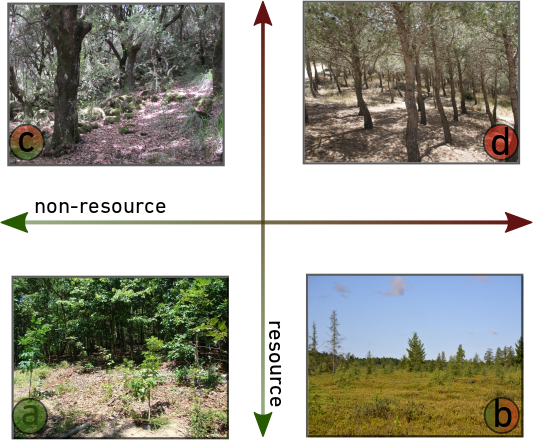
\includegraphics[width=\textwidth]{./Figures/chapter06/Fig_1.png}
\caption[Resource and non-resource environmental gradients]{\color{Gray} A two dimensional environmental gradient. In this example, the non-resource factor  is soil ph, and the resource factor is available direct sunlight. Considering a plant species with optimal fitness at basic ph levels and high levels of direct sunlight, the environmental gradients show different combinations of factors: (a) suitable light and ph levels may be found in open areas or forest gaps on basic soils, (b) peat bogs are highly acidic environments, but otherwise suitable regarding light levels, (c) closed canopies under basic soils may have too low light levels, (d) understoreys of pine forests have both low light levels and acidic soils.}
\label{fig:fig6.1}
\end{figure}

\section{Methods}

\subsection*{Modelling community responses to a combined gradient}

The basic tenets presented above apply, all else being equal, to gradients of only one factor at a time. However, it is harder to derive conceptual predictions about variations across combined gradients of both types. Using a simple community model, we analysed whether variations in two environmental factors, a resource and a non-resource one, drive variations in different patterns of a horizontal community (composed of a single trophic guild). We generated a pool of species with varying demographic responses to non-resource stress factors, following the functional responses discussed in \cite{Maestre2009}, in which species vary their survival and growth rates according to the level of non-resource stress (Appendix 6.1). The two extreme cases in this framework are, on the one hand, stress-tolerant species, that are able to maintain comparatively high survival rates under high stress levels, but display lower growth rates in the absence of stress; and competitive species on the other hand, that show high growth rates under benign conditions but also higher sensitivity in both survival and growth rates to non-resource stress.

In our model setting, environmental variability is represented by a two-dimensional lattice, in which each cell has a combination of resource and non-resource environmental factors (\cref{fig:figApp6.1.1}). The resource factor is represented as the carrying capacity of the cell, and all species are assumed to belong to the same trophic guild (sensu \citealt{Fauth1996}), whose only limiting factor is that resource. The non-resource factor is homogeneous and constant in a given cell. Both gradients are linear.

Species randomly colonize with equal probability any given cell of the lattice, and survive and grow according to their specific functional responses (\cref{fig:figApp6.1.2}). A fraction of species is able to facilitate the survival of heterospecifics, by enhancing their survival probability in the face of high levels of non-resource stress. The intensity of each facilitation event is given by the biomass of the benefited individual, that would have otherwise not survived.

Individuals in a cell are able to grow up to the level where their aggregated biomass equals the carrying capacity of the cell, i.e. the level of resource factor. Competition occurs when the growth of one or more individuals is hampered due to the presence of another individual, and its intensity is given by the amount of expected growth that was impeded by the competitive exclusion.

With this simple setting, we modelled how species interact and persist through time in each combination of the two gradients. After an initial warm-up period of 100 timesteps, to allow each cell to be colonised, we recorded for 500 timesteps every facilitative and competitive interaction, the effective number of species at each cell (also known as “Hill number” or “true diversity”, \citealt{Tuomisto2012}), and the average persistence time of species at each cell. To evaluate the response of these metrics to the environmental gradients, we fitted generalised additive models (GAMs) to the results from our simulations. Generalised additive models use smoothing functions to model nonlinear relationships, providing a flexible nonparametric model \citep{Wood2017}. Given the strong nonlinearities observed in our responses, we fitted GAMs with adaptive smoothing terms, that are able to model responses where the degree of smoothness vary over the range of the covariates \citep{Wood2017}.

We also performed simulations with the same parameterization but not allowing for facilitation, and compared the distributions of competition intensity, species diversity, and persistence times in the two sets of simulations, using Wilcoxon signed-rank tests.

\section{Results}

\subsection*{Does the intensity of competitive and facilitative interactions vary across a combined resource and non-resource environmental gradient?}

The intensity of competition and facilitation strongly varies across the combined environmental gradient (Fig. \ref{fig:fig6.2}, Table \ref{tab:tab6.1}). Competition intensity increases with increasing resource stress (Fig. \ref{fig:fig6.2}, panel a) and with decreasing non-resource stress (Fig. \ref{fig:fig6.2}, panel b), and the interaction between resource and non-resource stress is also statistically significant (Table \ref{tab:tab6.1}). Facilitation intensity, in turn, is only significantly influenced by non-resource stress (Table \ref{tab:tab6.1}, Fig. \ref{fig:fig6.2}, panel c and d). In absence of stress, there is no facilitation, as every species has a survival probability of 1 (\cref{fig:figApp6.1.2}). Then, as non-resource stress increases, facilitation intensity displays a concave parabolic shape: it is high and very variable for low levels of stress, lowest for intermediate levels, and consistently high and comparatively less variable for high stress levels.

\clearpage
\begin{landscape}
\begin{table}[] \footnotesize
\caption[GAM model results]{\color{Gray}Results of the Generalised Additive Models fitted to the simulation results. REML = Restricted maximum likelihood. For parametric coefficients, their estimates, standard errors, and t-statistic are given, whereas for smooth terms, we report their estimated degrees of freedom (edf), and their F-statistic.}\label{tab:tab6.1}
\begin{tabular}{lllllllllll}
\hline
Response                                                                               & REML                     & $r^{2}$ & Deviance                & Covariates               & Estimate  & Std.Error  & t      & edf   & F      & p-value        \\
\hline
\multirow{3}{*}{\begin{tabular}[c]{@{}l@{}}facilitation\\ intensity\end{tabular}}      & \multirow{3}{*}{-1376.2} & \multirow{3}{*}{0.528}   & \multirow{3}{*}{53.1\%} & intercept                & 0.674     & $6.3*10^{-3}$ & 106.56 & -     & -      & $< 0.05$ \\
                                                                                       &                          &                          &                         & resource                 & $-4.8*10^{-5}$ & $1*10^{-4}$     & -0.465 & -     & -      & 0.642          \\
                                                                                       &                          &                          &                         & s(non-resource)          & -         & -          & -      & 14.16 & 167.5  & $< 0.05$ \\
\multirow{4}{*}{\begin{tabular}[c]{@{}l@{}}competition\\ intensity\end{tabular}}       & \multirow{4}{*}{-5459.3} & \multirow{4}{*}{0.967}   & \multirow{4}{*}{96.7\%} & intercept                & 0.108     & $5.2*10^{-4}$   & 208.4  & -     & -      & $< 0.05$ \\
                                                                                       &                          &                          &                         & s(resource)              & -         & -          & -      & 3.28  & 7405   & $< 0.05$ \\
                                                                                       &                          &                          &                         & s(non-resource)          & -         & -          & -      & 12.53 & 1813.5 & $< 0.05$ \\
                                                                                       &                          &                          &                         & s(resource*non-resource) & -         & -          & -      & 25    & 262.4  & $< 0.05$ \\
\multirow{3}{*}{persistence times}                                                     & \multirow{3}{*}{7451.8}  & \multirow{3}{*}{0.986}   & \multirow{3}{*}{98.6\%} & intercept                & 26.18     & 0.217      & 120.71 & -     & -      & $< 0.05$ \\
                                                                                       &                          &                          &                         & resource                 & $2.2*10^{-3}$  & $3.5*10^{-3}$   & -0.625 & -     & -      & 0.532          \\
                                                                                       &                          &                          &                         & s(non-resource)          & -         & -          & -      & 14.29 & 10741  & $< 0.05$ \\
\multirow{3}{*}{\begin{tabular}[c]{@{}l@{}}effective number\\ of species\end{tabular}} & \multirow{3}{*}{4127.2}  & \multirow{3}{*}{0.922}   & \multirow{3}{*}{92.2\%} & intercept                & 4.828     & 0.057      & 83.92  & -     & -      & $< 0.05$ \\
                                                                                       &                          &                          &                         & resource                 & -0.016    & $9.4*10^{-4}$   & -16.64 & -     & -      & $< 0.05$ \\
                                                                                       &                          &                          &                         & s(non-resource)          & -         & -          & -      & 10.36 & 2355   & $< 0.05$
%\hline
\end{tabular}

\end{table}
\end{landscape}

\subsection*{How are species diversity and persistence affected by the environmental variation?}

The effective number of species at each cell drops rapidly with even slight increases in non-resource stress (Fig. \ref{fig:fig6.2}, panel f), and also shows a decreasing trend, although less steep, with increasing resource stress (Fig. \ref{fig:fig6.2}, panel e). Average persistence time, in turn, also decreases very sharply with non-resource stress (Fig. \ref{fig:fig6.2}, panel h), but is unaffected by resource stress (table \ref{tab:tab6.1}, Fig. \ref{fig:fig6.2}, panel g).

\subsection*{Does the presence of benefactor species increase species diversity and persistence in our model communities?}

Both species diversity and persistence times are significantly higher in simulations with facilitation (Table \ref{tab:tab6.2}, \cref{fig:figApp6.1.4}).

\begin{table}[]
\caption[Facilitation impacts]{\color{Gray}Results of the Wilcoxon signed-rank tests for differences in competition intensity, species diversity, and average persistence times between communities with and without facilitation. Test on competition intensity is two-tailed, reflecting our lack of previous hypotheses on the intensity of competitive effects between the two sets of simulations. Tests on species diversity and persistence are one-tailed, with the alternative hypothesis being greater values of both metrics when facilitation is allowed. In bold, highest median values of each quantity.}\label{tab:tab6.2}
\begin{tabular}{lllll}
\hline
 & median - facilitation & median - no facilitation & V & p-value \\
\hline
\begin{tabular}[c]{@{}l@{}}competition\\ intensity\end{tabular} & \textbf{0.059} & 0.050 & 1229233 & $< 0.05$ \\
persistence time & \textbf{15.47} & 12.369 & 2401500 & $< 0.05$ \\
\begin{tabular}[c]{@{}l@{}}effective number\\ of species\end{tabular} & \textbf{2.374} & 2.067 & 2600200 & $< 0.05$
%\hline
\end{tabular}

\end{table}

\begin{figure}[ht]
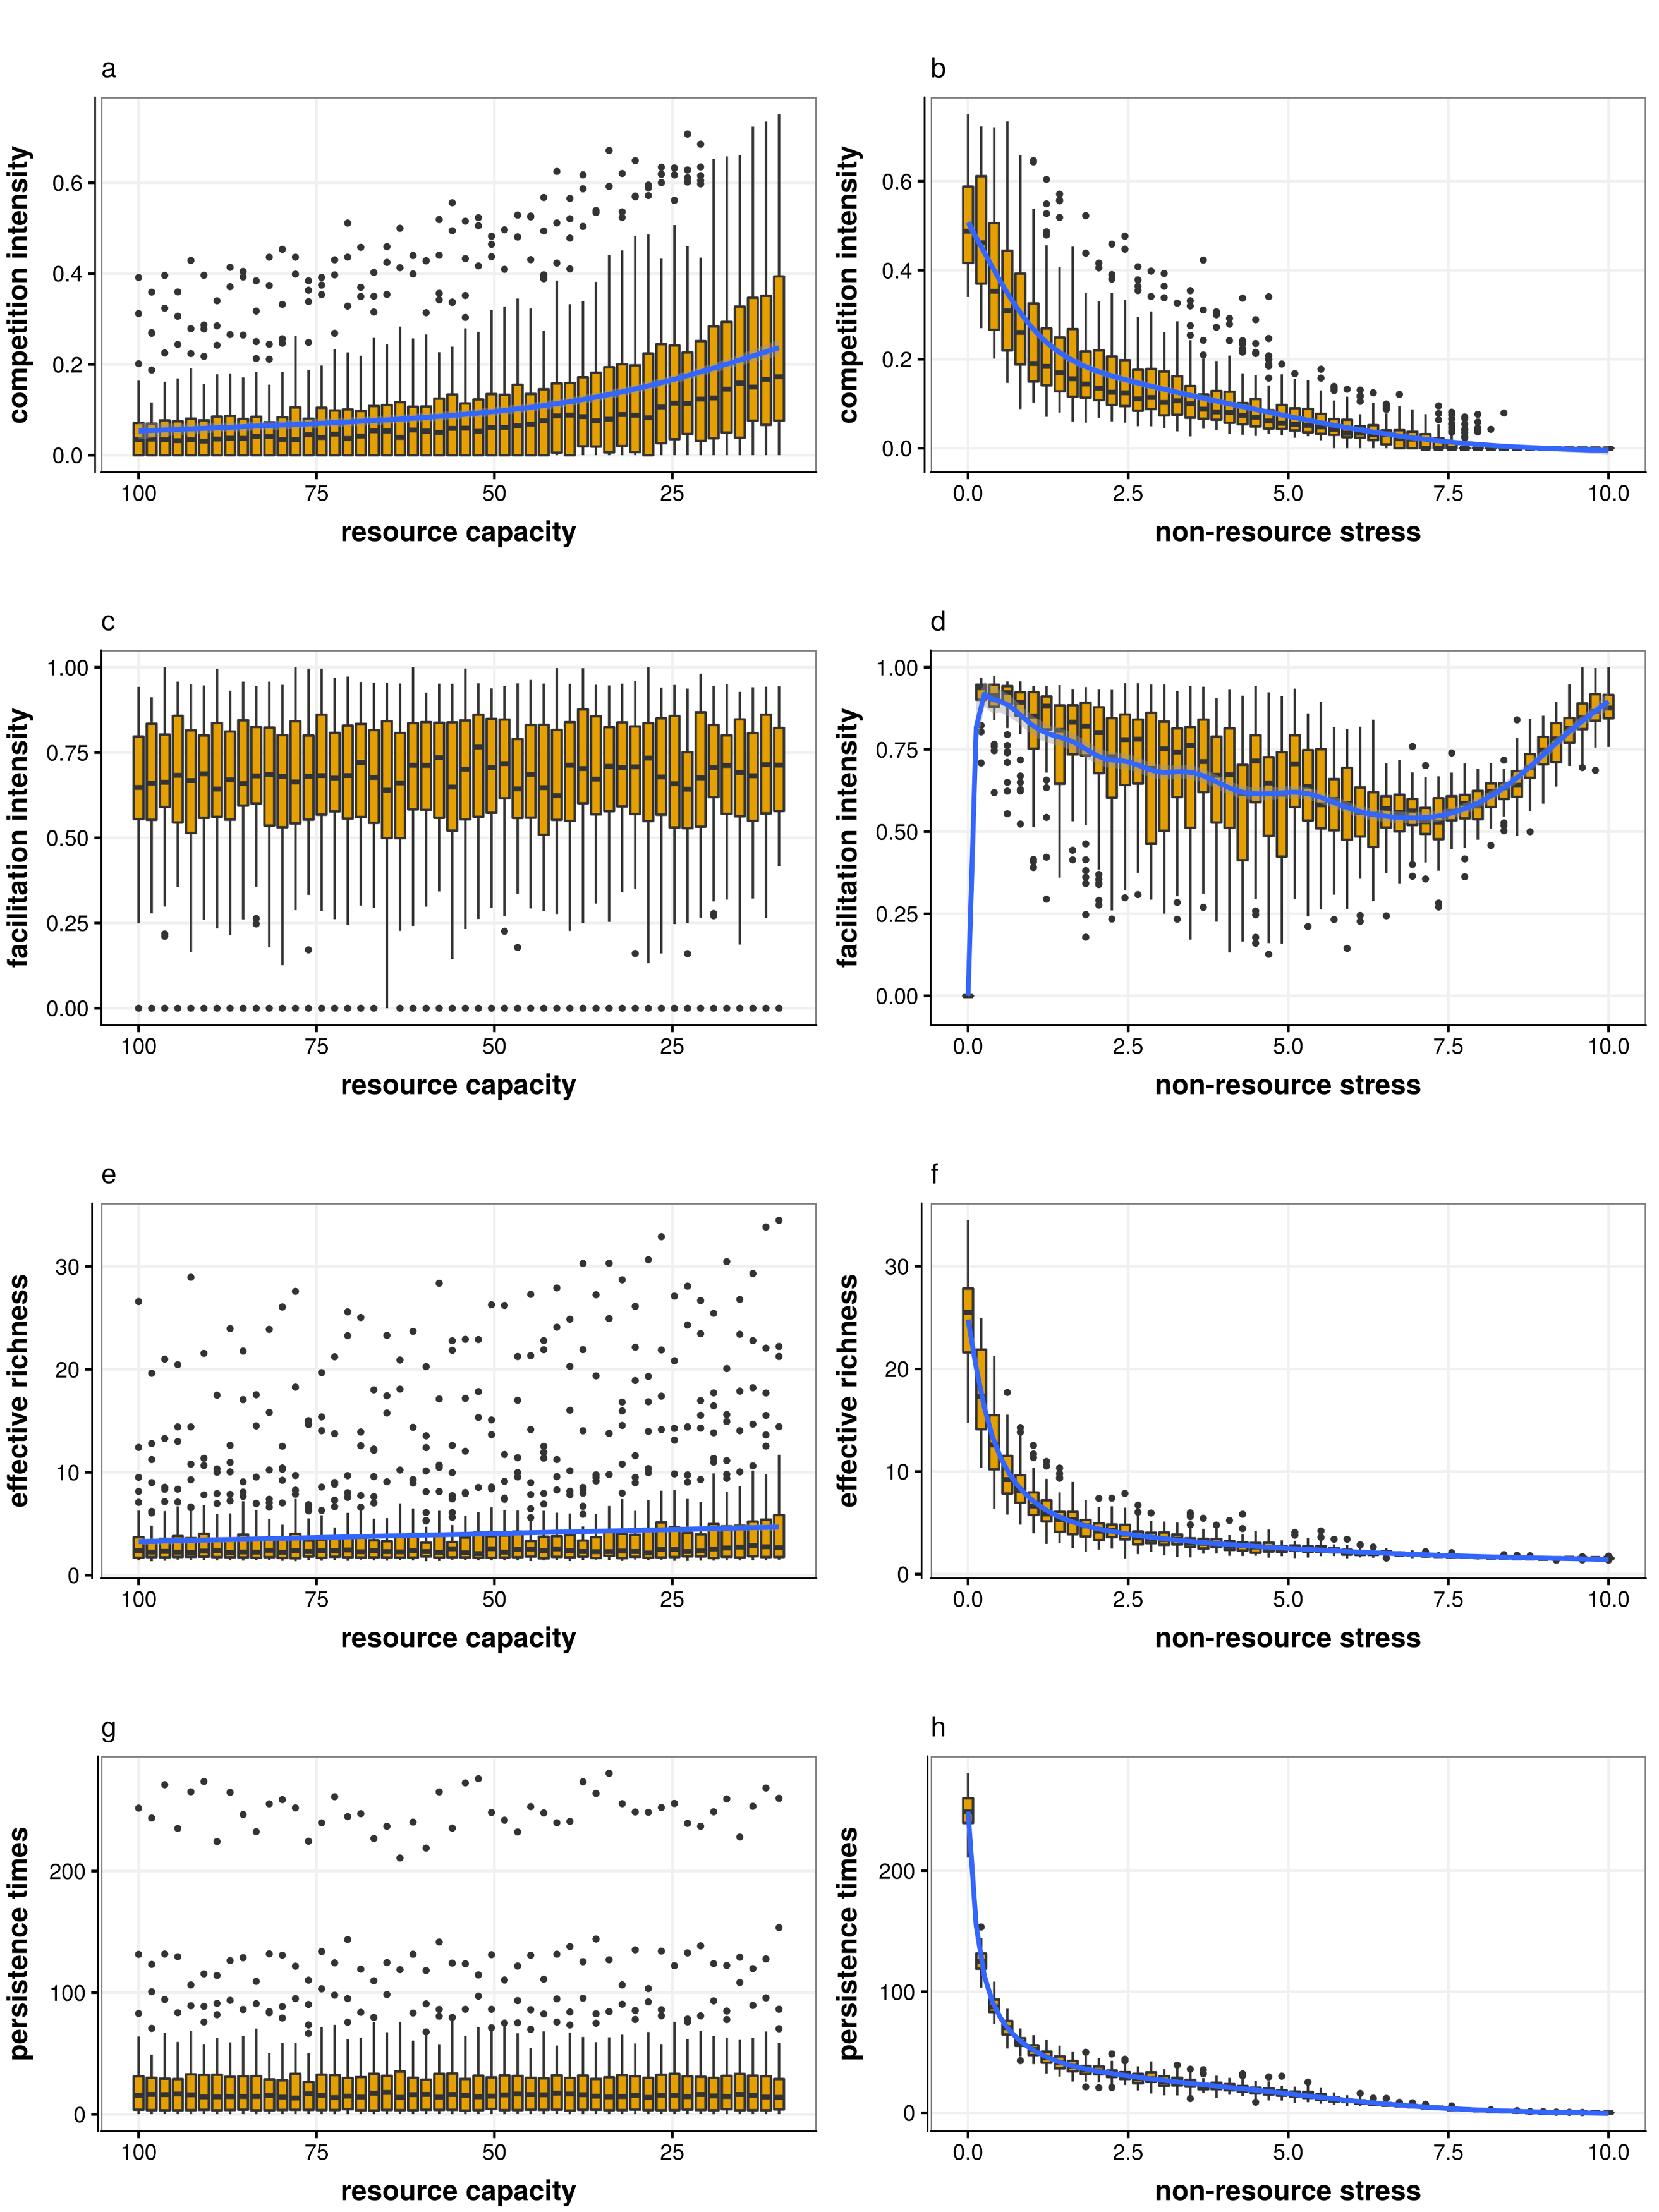
\includegraphics[width=\textwidth]{./Figures/chapter06/Fig_2.png}
\caption[Community responses to gradients]{\color{Gray} Variation of community-level properties across a resource and a non-resource gradient. For variables selected as significant by the GAM models (Table \ref{tab:tab6.1}), model fits are superimposed as blue curves.}
\label{fig:fig6.2}
\end{figure}

\section{Discussion}

We modelled the response of species ranging from pure competitors to pure stress-tolerance within a two-dimensional environmental gradient combining a resource and non-resource factor. The two types of environmental factors have contrasting influences on (1) the intensity of pairwise interactions and (2) the diversity of species in the community and their average persistence times.

The intensity of competitive interactions clearly increases with increasing levels of resource stress, as expected. However, it also increases for decreasing levels of non-resource stress. This is due to the positive correlation observed between mortality rates and non-resource stress, that releases resources and decreases effective competition at highly stressful environments.

Facilitation is, again as we hypothesised, clearly driven by variations in the non-resource factor. The response observed is, however, more complex than the standard expectations derived from the stress-gradient hypothesis, that predicts either an increasing importance of facilitation with increasing stress, or an increase followed by a collapse in facilitation levels at very high stress levels \citep{leRoux2010}. The idea behind this latter version of the theory is that in extremely harsh environments, the facilitation effect of nurse plants is severely hampered \citep{Michalet2006}. This reasoning, however, only applies to non-resource factors, as species do not compete for them; if the environmental gradient includes resource factors, net interaction effect may switch from positive to neutral or negative \citep{Smit2007,Michalet2014}. In our simulations, we first observed, as expected, no facilitation in the absence of non-resource stress. As soon as there is a certain environmental impact on competitive species, however, facilitation sharply increases, while at the same time showing a high variability. We argue that this unexpected variability is due to priority effects, in which the order of arrival of species to a location is an important factor for the subsequent dynamics of the local community \citep{Fukami2015}. In our model, all species have the same probability of colonizing any cell of the grid: if the first colonizers are facilitators, follow-up colonizers will likely experience some degree of facilitation as long as stress levels are not null. On the other hand, facilitation will be residual if the early colonizers are able to thrive in the location but do not facilitate the establishment of other species. Following the environmental gradient, If non-resource stress increases, stress-tolerant species will be progressively selected for, and competitive species will only persist when facilitators are present. At very high stress levels, survival probability is extremely low for all species, so most surviving individuals are subject to a certain degree of facilitation. It is important to note that, in our model, facilitation capacity does not decrease with increasing stress, as may occur for example in grazing gradients \citep{Smit2007}. We also note that we explicitly modelled locations with unlimited potential colonizers from the same regional species pool, in order to isolate effects arising directly from environmental constraints on response curves, and discard species-pool effects (e.g. \citealt{Partel1996}).

In this first approximation to the concurrent modelling of resource and non-resource environmental gradients, we defined a single resource factor as a carrying capacity, and did not account for more complex relationships that allow facilitation of resource factors. For example, it is well established that, although species compete for water in stressful environments, nurse species can facilitate water acquisition by heterospecifics under different circumstances, listed in \cite{Maestre2009}: by lifting water from belowground, by providing shade that retains moisture, and, again as a byproduct of shade provision, by modifying water-relations of the understorey species. Aside from the important example of water, it is nevertheless clear that most resource factors shared by species of a certain guild (i.e. light, space, nutrients) are generally not facilitated by species of that guild, and hence the prevalence and intensity of facilitation should, in most cases, conform to the hypothesis laid out here.

Species diversity and persistence are highly sensitive to variations in the non-resource factor, and this is mainly due to the shape of the physiological responses to non-resource stress that we modelled (\cref{fig:figApp6.1.2}). Less steep declines in survival or growth probability would smooth the responses to increasing stress. We carried out additional simulations (not shown here) and observed that higher variation between purely competitive and purely stress-tolerant species did indeed increase the steepness of the diversity and persistence responses. Nevertheless, the overall trends were qualitatively robust to the different parameterizations, and should hold as long as competitive species are comparatively more sensitive to stress.

Despite facilitation being present at high levels of non-resource stress, species diversity and persistence time both decrease consistently across the non-resource gradient: the negative effects on growth and survival across the species pool are stronger than the benefits of facilitation by stress-tolerant species. Facilitation does, however, increase competition intensity, species diversity and persistence times overall (Table \ref{tab:tab6.2}), with its strongest influence occurring at low to moderate levels of non-resource stress (\cref{fig:figApp6.1.4}).

In our model, we considered a single non-resource environmental factor and a single resource that is utilised equally by all species and does not deplete. Of course, the picture is much more complex in natural systems, where species consume several resources with varying efficiencies \citep{Chapin1987} and may display contrasting physiological response curves to different non-resource factors \citep{Austin1994}. Furthermore, we are considering here horizontal communities, and the responses discussed will likely be more complex for multi-trophic communities and involve direct and indirect effects on community properties \citep{Menge1987,Bruno2003}. We expect that in communities comprising several guilds and potentially different types of interactions among species, variations in non-resource factors will (1) directly affect all species regardless of their position in the community, and (2) those effects will not be homogeneous. In particular, it is expected that species up in the trophic chain will be comparatively more sensitive to environmental variability \citep{Voigt2003}. Therefore, as a first hypothesis, we suggest that non-resource environmental gradients will trigger both direct effects on all trophic guilds and also significant top-down indirect effects on community structure and dynamics. In turn, variations in resource factors can be expected to affect more significantly lower trophic levels, since species of higher trophic levels get most of their nutrients from direct consumption of organic matter from lower trophic levels. As such, we hypothesize that the most important effect on community structure and dynamics across non-resource environmental gradients will be through bottom-up control.

Despite the simplicity of our model, we have clearly shown that the two general types of resource and non-resource environmental factors differentially influence biotic interactions, species richness and persistence in model communities. Several fundamental questions arise from these results. The spatial scale of different environmental gradients, for example, should interact with the spatial signal of the different interaction types \citep{Araujo2014} to influence large-scale persistence and diversity patterns. Even at local scales, integrating the different aspects of environmental variability with established frameworks such as the resource ratio theory or modern coexistence theory should bring novel insights for the influence of environmental gradients on ecological communities.

%
%************************************************
\chapter{General discussion and conclusions}\label{ch:discussion}
%************************************************

\tikz[remember picture,overlay] \node[opacity=0.3,inner sep=0pt] at (current page.center){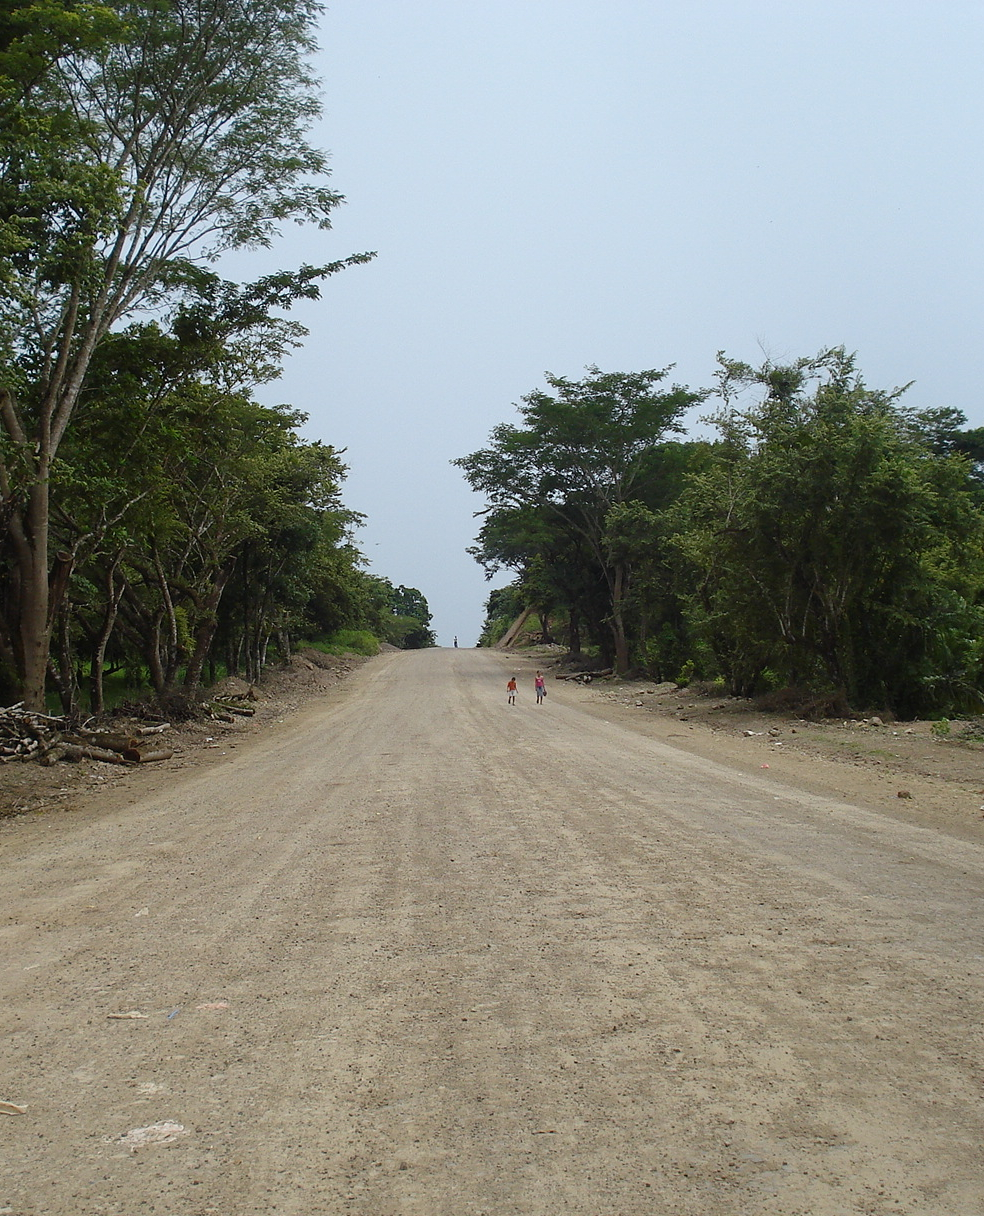
\includegraphics[width=\paperwidth,height=\paperheight]{./Figures/cover/carretera_nica_pagina.jpg}};
\clearpage

We live in a time in which global environmental changes are occurring at unprecedented scales and speeds \citep{Pachauri2015}. Individual species and whole ecological assemblages face systemic risks from a variety of stressors, including the loss and fragmentation of suitable habitat, alterations in the temperature and precipitation regimes, pollution, or an increase in the rate of colonization of human-borne potentially invasive species \citep{Vitousek1994}. Given the scale and magnitude of the human alteration of the environment, it is urgent to develop mitigating measures at all levels, from actions in local habitats to coordinated worldwide socioeconomic efforts that bring us closer to a harmonious coexistence with the non-human world. In order to move towards this admittedly utopian objective, we need the strongest possible scientific understanding of how ecological species and communities are structured, and how they function. In a testimony to the complexity of the natural world, our knowledge of ecological communities is still limited, despite decades of continued work by generations of naturalists and ecologists. In particular, we do not know whether pairwise interactions between individuals are structured in order to enhance community stability sensu lato. When certain interactions are considered in isolation, e.g. trophic or mutualistic ones, theoretical \citep{Williams2000} and empirical \citep{Thebault2010} studies have shown that interactions are indeed distributed non-randomly. However, species in ecological communities display a wide array of interaction types and mechanisms, and we are only starting to gain a broad understanding of how the different interactions combine in natural systems \citep{Kefi2015}, and its implications for ecological processes \citep{Pocock2012}.

In this thesis, I have explored several fundamental questions about networks of ecological interactions, their structure and dynamics in different contexts. In the following paragraphs, I discuss some of the main findings of the thesis and potential lines of work arising from them, in light of the current literature knowledge.

There are only a handful of empirical datasets that account for multiple interaction types in ecological communities (chapter 2). It is therefore only logical that most studies that analyse these complex networks are theoretical in nature, but even restricting ourselves to theoretical models for building and analyzing multiple interactions networks, the diversity of approaches and objectives is already substantial. I have shown that, on a conceptual level, this diversity of modelling strategies boils down to three types of approaches (chapter 2). This conceptualization may help researchers design theoretical studies with a clearer understanding of the limitations and strengths of the methodologies used. For example, not all interaction types occur in the same spatial and temporal scales. Models that lump together interaction effects in a single parameter and do not differentiate spatiotemporal patterns (such as the model developed in chapter 3) should be very explicit about these limitations, and in any case, should be considered baseline models, potentially useful for (1) guide further, more targeted theoretical and empirical work, and (2) comparison against more realistic models. Looking at the broad picture, one may ask whether the increase in model complexity and data collection programs necessary for accounting for different interaction types is worth it, i.e. if it significantly improves our understanding of ecological communities. Although the field is still young, and all conclusions are based on highly idealized models or on very specific, likely incomplete datasets, current results suggest that, indeed, integrating the variety of interactions present in nature into the study of ecological networks produces novel insights and unexpected outcomes, regarding for example the patterns of secondary extinctions in networks \citep{Pocock2012,Evans2013a}, the functional groupings in communities \citep{Kefi2016a}, or, as shown in chapter 3, the persistence of species in their local communities. It remains to be seen, however, if a truly consistent program of data collection across different community types and environmental gradients is feasible, or how more modest experiments such as microcosms can be designed for taking full advantage of this view of ecological communities.

As stated above, before we can extract robust conclusions from empirical data, we may advance our understanding of multiple interaction networks by developing general, overarching models and theories. With that objective in mind, I developed the model of chapter 3, and in its design, I brought together a series of separate insights about interaction networks. In particular, the way in which interactions are quantified is based on the assumption that the abundance of the interacting species is related to their interaction frequency: the more abundant the two species are, the more will they interact. Interaction frequency is, in turn, taken as a measure of the impact of one species over another. This assumption has been corroborated for a number of plant-pollination networks \citep{Vazquez2005,Vazquez2007,Vazquez2012}, but it probably does not hold generally for all interaction types, and it explicitly neglects specialization in ecological interactions. Nevertheless, it represents a robust approach for integrating with a single currency the effects of disparate interaction types in dynamic models.

The results from chapter 3 open different avenues for future research. The most straightforward extension would be the development of experimental or observational studies for testing some of the results: in particular, it would be feasible to test whether species-poor communities tend to have a higher prevalence of positive interactions, as suggested by our theoretical results, and how are these interactions distributed. The assumption that interactions are distributed non-randomly proved key for maintaining high levels of persistence: even in species-poor communities, interactions should maintain a certain structure. Such targeted empirical work could also start to unveil the frequency and structure of less studied interactions. Amensalism and commensalism have been shown in another recent study to improve community stability when accounted for \citep{Mougi2016a}, but they are clearly underrepresented in the literature. Another theoretical outcome from that chapter that would require further study is the observed relationship between the frequency of occurrence of the different interaction types and their connectance values (Appendix 3.4). As long as the set of feasible potential links varies for the different types of interaction, frequency of occurrence and connectance will not be equivalent. I believe that the calculation of connectance relative to fully connected networks should be approached with caution, as there are countless examples in which many of the potential interactions are forbidden because of, for example, non-overlapping activity in time or space \citep{Yang2010,Osorio2018}. In any case, it is unlikely that in multitrophic networks, the set of, say, potential mutualisms, would be the whole network. When evaluating more thoroughly structural metrics of multiple interactions networks, these details should not be overlooked. Note that, throughout chapter 3, I have purposely concentrated on species abundances and already established interactions. Trait-based approaches for inferring interactions \citep{Morales-Castilla2015, Bartomeus2016} and community structure \citep{Laigle2018} also show great promise, but they are difficult to generalize to different types of communities and habitats. It is probably not possible to derive a set of traits from which to predict the occurrence of different interactions, applicable across trophic levels and habitat types. But perhaps it is feasible to ask whether, in a general way, traits that are known to influence trophic interactions are also important in mediating other interaction types (e.g. are species of similar body sizes more likely to compete with each other?).

The only ``trait'' included in the model of chapter 3 is the trophic level of each species. From this separation of species into trophic levels, I found that the persistence values in different trophic levels were markedly different in the simulated communities (\cref{fig:figApp3.2.1}). This result prompted the question that would end up shaping chapter 4: if persistence levels in complex communities are affected by interaction type frequencies and network structure, other community-level patterns should also be affected. This question points to a more general feature of ecological thinking, discussed in chapter 4. Community ecology has, historically and for several reasons, concerned itself with communities of a single functional guild, whereas analyses of ecological networks followed a parallel path in which functional distinction among species is assumed seamlessly. Many highly influential theories in community ecology have been framed in terms of competition for resources within a certain guild (e.g. Tilman's resource ratio theory, Chesson's modern coexistence theory), and only recently the frame is expanding in order to account for interactions among functional guilds \citep{Chesson2008,Godoy2018, Seibold2018}. An implicit objective of chapter 4 was to advance in this expansion of classic community ecology patterns into multi-trophic communities with potentially complex network structures. The most important message from chapter 4 is that context matter, and many factors interact when trying to elaborate how patterns vary across trophic guilds. We are not yet even close to a conceptual theory of community ecology of complex ecological networks, but this and the aforementioned studies are steps towards that goal.

In chapter 5, I delved deeper in that overarching objective of advancing community ecology for multi-trophic communities, this time focusing on the spatial dimension of interactions. Metacommunity theory has provided very important insights in the functioning and dynamics of spatially-connected communities. Again, most of this framework has revolved around two key assumptions: communities are horizontal, comprised of a single guild of species that compete among them, and these discrete communities are conected by dispersing individuals. After almost two decades of work, recent studies started to expand the paradigm of metacommunity ecology in different ways, e.g. considering more complex communities or integrating different forms of individual and material connections between communities. We opted for combining both extensions to classic metacommunity theory, and found that, as could be intuitively expected, when species forage into different patches, interaction dynamics clearly differ from the dispersal case. Spatial effects are propagated generally up to four or five links in the metacommunities of our general model, an insight that, if it holds, could have conservation implications for instance for evaluating the regional impact of species introduced in a limited number of localities.

Arising from the model of chapter 3, a prominent question we faced was how could we generate frequencies and topologies of interaction types that were realistic, or at least approaching some degree of realism. We ended up doing a literature review on how the different interaction types occurred across different trophic levels, but this is only an ad-hoc solution for that particular study. In order for studies on multiple interactions to advance, robust knowledge on the frequency and topology of different interactions across environmental gradients and community types is sorely needed. This prompted the research of chapter 6, which matured in a fairly different way from that original idea. Originally, we expected to generate predictions of interaction frequencies in communities based on environmental or other constraints (imagine a world map with regions differentiated by the prevalence of the different interaction types, e.g. mutualism-dominated communities or predation-dominated ones). This, however, proved too demanding given the limited time frame of a Ph.D. project and the absolute lack of data. I resorted to study horizontal communities, and quite early realized what is now the core idea from chapter 6: that environmental factors are very different from one another and this differentiation should be better reflected in studies of ecological patterns across gradients. In that chapter, I only hint at what the effects of different gradients could trigger in more complex communities, but this line of research is potentially among the most important ones arising from the Ph.D.

A common theme to all chapters is the reliance on simulation methodologies to infer ecological insights applicable beyond the simple systems modelled. Numerical simulations allow a greater degree of model flexibility and complexity than analytical derivations, but of course it is harder to pinpoint the importance of the different model parameters, given their higher number and the difficulty of performing exhaustive sensitivity analyses. An important strength of simulation methods is that they allow the explicit inclusion of stochasticity on the model system, as I have tried to include in all the models developed. Interactions and functional relations in ecological communities are probabilistic in nature, rather than fixed, and I tried to keep that in mind in all the outcomes of the thesis. Given the nature of the questions asked in this thesis, I was not able to test most of the theoretical predictions against empirical data. This divide between theory and empiricism is a long-standing problem in ecology, perhaps more so than in other disciplines, and is discussed in detail in each chapter. It was my intention, however, to develop theoretical models with an eye on potential follow-up tests in natural systems. Therefore, in the following section, I advance in more detail how the chapters in this thesis could be complemented by experimental or observational studies.

\subsection*{Empirical observations, experiments, and applications}

The adequate sampling of ecological networks is a key issue in community ecology \citep{Jordano2016}, with important consequences for assessing the functional role of species within a network or the relative prevalence of rare and weakly-interacting species. In chapter 2, we discuss the main strategies employed so far for collating networks with multiple interaction types. These can be summarized as follows: a first alternative is to join together data from different sources and generate an inferred network; a second alternative is to develop comprehensive sampling programs of different functional groups and interaction types of specific communities. In both cases, the conceptual and logistic problems are potentially important. For example, when mixing data from different sources, one must make sure that there are no biases associated with the spatiotemporal extent of the sampling, or at least, incorporate these dimensions in the analysis (see chapter 4). This is particularly important for functional groups which are likely to have very different home ranges and dispersal distances.

Perhaps the most straightforward way of sampling complete networks is to resort to artificial mesocosms or natural communities with relatively few species or interactions (e.g. the Aire Island in chapter 2, or the core interactions in a mediterranean forest community studied by \citealt{Sunyer2016}). However, in all these scenarios there remains the issue of correctly documenting and quantifying direct interactions of different types, a discussion that has developed independently in food web studies \citep{Berlow2004, Wootton2005, Novak2010}, networks of competitive interactions within a single trophic level \citep{Freckleton2009a, Hart2018}, and mutualistic networks, mainly plant-pollinator ones \citep{Vazquez2005,Vazquez2007,Holland2002}. Virtually no empirical study that I am aware of has quantified the importance of one-way interactions (amensalism and commensalism) or has compared the relative importance of different interaction types in a single multi-trophic community, although recent calls for integrating multi-trophic approaches in community ecology are appearing: alongside this thesis, see for example \cite{Seibold2018}. An adequate sampling, in communities across environmental gradients, of (1) abundances and traits such as body size of species from key functional guilds, including parasites/parasitoids \citep{Lafferty2006}, (2) interaction frequencies and/or per capita strengths, is the golden standard to which we should move forward. Such data, when appropriately replicated, could easily corroborate or refute many of the ideas presented in chapters 2, 3, 4, and 6 of this thesis. As stated above, one way to approach this challenging program is through the use of artificial mesocosms, which allow the deployment of many types of experimental designs with appropriate control types, for example varying environmental or nutrient-input gradients \citep{Moss2004}, community assembly \citep{Chase2007, Jiang2008}, or colonization rates \citep{Fahimipour2014}. By establishing pond mesocosms along, for example, a warming gradient and a complementary nutrient-input gradient, the effects of the environment on interaction importance could be measured (chapter 6), and the short-term persistence of species (chapter 3) as well as the distribution of abundances of the different trophic guilds (chapter 4) could be quantified.

The spatial propagation of interactions in metacommunities connected by dispersal and foraging would require slightly more elaborate experimental designs. In particular, foraging requires species dwelling at a reproductive site that eventually move to feed in other localities. In order to test the differential effects of a foraging species in its home location and in other local communities, long-term experiments relative to the generation times of the species should be set up, and if artificial mesocosms were to be used, the different localities should be connected by a matrix allowing movement at least in a linear fashion. Furthermore, local communities should be set so as to prevent the establishment of the forager species in sites other than its home site. For example, predatory fish with specific needs for their reproductive sites could be introduced in mesocosms engineered with the appropriate characteristics for their breeding, while at the same time connecting these home mesocosms to other ones in which fish could eventually forage but not breed.

All these proposals are at this moment speculative, but feasible given appropriate projects and time frames. In the more general topic of how the insights from this thesis and its potential follow-ups could benefit applied ecology, it is relevant to note that the spatial scales in which ecologists define ecological communities and metacommunities are coherent with the scales at which local conservation and restoration projects are carried out. For example, quoting \cite{Wainwright2017}: ``Community ecology theory has particular relevance to restoration because it describes the processes that underlie the assembly, maintenance of diversity and functioning of ecological communities, which are often the focus of restoration projects''.

Insights on species persistence (chapter 3), the distribution of species abundances (chapter 4) and their spatiotemporal variation are key for preserving ecosystem functioning and diversity. In particular, a network perspective to conservation and restoration ecology is urgently needed. As \cite{Harvey2017} notes, species interactions must be taken into account when assessing conservation priorities, due to the interdependencies and feedbacks that arise from direct and indirect interactions. Often, as it has been shown previously \citep{Menge1995,Suttle2007,Montoya2009a} and in chapter 5 of this thesis, the net effect of interactions can reverse the expectations from direct interactions or from environmental constraints. Thus, preserving interactions appears to be as important as preserving keystone species, in order to maintain both community structure and function \citep{Wang2018}. In turn, the variability of interaction occurrence and outcome along environmental gradients is still hardly known \citep{Poisot2017}, and more empirical work is necessary on a variety of systems and interactions.

Throughout this thesis, I have stated the need for more directed, long-term empirical efforts in order to improve our basic knowledge of ecological communities and their mechanisms. Maintaining a balance and a healthy dialogue between theoretical research and applied ecology is by all means necessary if we are to help mitigate the current biodiversity crisis. Hopefully this thesis will contribute to that objective.

\subsection*{Conclusions}

\begin{itemize}
  \item \textbf{Chapter 2:}
  \begin{itemize}
    \item There is a high diversity of objectives and methodologies for studying ecological networks with multiple interaction types. Despite this variability, most theoretical approaches can be reduced to three conceptual methodologies. Multilayer networks are the most general one, and the other two methodologies can be seen as special cases of multilayer networks, that focus on different aspects of the interaction network.
    \item The three methodologies proposed are best suited to different types of interaction data, and to different objectives. The single most important issue we face in the study of multiple interactions networks is the lack of robust data for a variety of communities and habitat types.
  \end{itemize}
  \item \textbf{Chapter 3:}
  \begin{itemize}
    \item In model communities, species persistence is highly influenced by the frequency and distribution of interaction types. In particular, the prevalence of positive interactions is significantly related to persistence in species-poor communities. In richer communities, this relationship is diluted, and different combinations of interaction frequencies are able to maintain high levels of persistence.
    \item Structural properties of the model networks are also important for species persistence, in the sense that more structured communities are more persistent. Furthermore, the simulated communities display emergent structural properties also found in empirical food webs.
  \end{itemize}
  \item \textbf{Chapter 4:}
  \begin{itemize}
    \item The distribution of abundances varies between guilds of terrestrial plants and mammals. In particular, abundances of terrestrial plants tend to be significantly less even and more skewed than those of mammals. Variations in competitive exclusion among guilds due to differences in niche availability may partly explain these trends.
    \item The patterns among consumer guilds are qualitatively similar to those predicted by simple theoretical models, and are mediated by other interacting factors such as the richness of the guild under study, the temporal and the spatial extent of the data acquisition scheme.
  \end{itemize}
  \item \textbf{Chapter 5:}
  \begin{itemize}
    \item The spatial propagation of interaction effects across local communities has a different signature depending on whether localities are connected by dispersing or foraging organisms. When local communities are connected by foraging, the net effects between any pair of species are much less predictable from local dynamics than in the dispersal case.
    \item The spatial decay of interaction effects follows a similar curve regardless of the type of movement between communities. Most interactions have a net effect on species up to five links away from the interacting pair, but rarely more.
  \end{itemize}
  \item \textbf{Chapter 6:}
  \begin{itemize}
    \item Environmental factors have different effects on species dynamics and interactions depending on whether they are consumed by species (resource factors) or not (non-resource factors). In particular, variations in non-resource factors drive gradients in facilitation intensity, whereas resource factors are the main driver of gradients in competition intensity. Other properties at the community level are also affected by these environmental gradients: species diversity and persistence times are mainly driven by variations in non-resource factors, with small effects from resource factors.
    \item The distinction between resource and non-resource factors is likely to be even more important for communities with several functional or trophic guids, as different factors affect differentialy the different guilds and potentially generate complex bottom-up and/or top-down dynamics.
  \end{itemize}
\end{itemize}


%************************************************
\chapter{Introduction}\label{ch:intro}
%************************************************

% switch between these depending on page size, or modify directly
% same for the rest of the chapters
%\tikz[remember picture,overlay] \node[opacity=0.3,inner sep=0pt] at (current page.center){\includegraphics[width=\paperwidth,height=\paperheight]{./Figures/cover/sesshu_1.jpg}};
\tikz[remember picture,overlay] \node[opacity=0.3,inner sep=0pt] at ([yshift=3cm,xshift=2cm]current page.center){\includegraphics[width=\paperwidth,height=\paperheight]{./Figures/cover/sesshu_1.jpg}};
\clearpage

\section{Community Ecology}

Humans have always marveled at the diversity of life forms on Earth. This fascination is reflected in the multitude of ways in which nature is represented and studied in the different branches of human knowledge. Some enjoy looking at the finest detail of the life histories of species and populations. To some of us, life forms are inherently self-organized into larger-scale structures that display their own rules and meaning; thus we look at a forest and see, indeed, a tight entanglement of individuals that cannot possibly thrive without the surrounding web of other species. Individual details, while extremely important, are embebbed into entities that posses their own ecological, aesthetical and etical relevance: ecological communities. While the Clementsian extreme view of communities as full-fledged, delimited entities capable of evolution and reproduction has long been abandoned, it is obvious that associations of individuals do generate predictable sets of processes and patterns, and the main concern of community ecology is with the discovery and understanding of these general processes and patterns. Community ecology is the discipline most directly concerned with the temporal and spatial scales at which individuals interact with each other. Processes intrinsic to this scale are generated by individual-level behaviours, that shape interaction patterns. Whatever the mechanisms by which such community-level patterns are driven, they feedback and influence individual life histories and, in turn, also biogeographic and macroecologic processes, such that the study of community ecology has an important relevance on its own and also plays a key role in understanding the emergence of global patterns from lower-scale processes.

Intuitively, an ecological community can be defined simply as a set of individuals that interact with each other. This broad picture needs to be refined when addressing the systematic study of these entities. For example, how do we define the \textit{set} of species that constitutes a community? What are the \textit{spatial} and \textit{temporal} limits of a given community? In the first chapter of this thesis, for example, we will encounter a community located on a small islet, in which a top predator is a bird of prey that can easily travel dozens of kilometers in a single journey and is thus not constrained by the territory of the islet, whereas other species are sessile or limited to ranges of a few hundreds of meters. Why would I include this top predator as part of the island community, when it clearly has a broader range than the rest of the species? And, looking at this question from another point of view, why would I \textit{not} consider as part of this community other species outside the islet that are also preyed upon by this predator?

The answer, as almost always in ecology, is that no fixed rules are applicable to all cases. Communities, despite their inherent structure and identity, are not organisms with closed physical boundaries to the outside world, and therefore, their spatiotemporal borders are extremely variable and are usually chosen ad-hoc by the investigators studying them. A great deal of studies in community ecology deal with so-called \textit{horizontal} communities. These are simply communities composed of organisms of similar characteristics, usually in terms of taxonomical relatedness. Thus, it is very easy to find studies about the \textit{grassland} communities of a steppe, or about the \textit{arthropod} communities present on the canopy of tropical trees. Such focus on certain groups of related species is necessary in order to understand in detail certain ecological processes and patterns, such as niche differentiation and coexistence among similar species. It is also very convenient in terms of experimental design, as it allows investigators to concentrate efforts on a small part of the enormous diversity present in every habitat. Studies on horizontal communities are at the core of classic community ecology, and we have learnt much about how species coexist with each other when resources are limited, about how species are positioned along environmental gradients, and about many other ecologically relevant questions.

Notwithstanding the importance and validity of the abstraction of horizontal communities, it is clear that they are somehow incomplete communities, if we recall the broad definition of community sketched above. No one can doubt that, in natural settings, the group of e.g. grassland species is interacting in many ways with other guilds: they are consumed by arthropod or mammal herbivores differentially, they may be pollinated by other sets of species, they may be affected by stamping of big animals or be fertilized by their dung. All in all, communities are more than disjointed taxonomic guilds, and their dynamics are influenced by the whole set of interactions occurring among their constituent species. The role of interspecific interactions is, then, key for understanding and predicting important ecological processes at this scale. It is this vision that has given rise to another long-standing branch of community ecology that has at its core the study of the interactions between different guilds or species within a community: the study of ecological networks. This thesis deals with complex communities represented as networks of interacting species, so I will give a brief overview of network theory in general and applied to ecological communities, and later introduce the specific questions addressed in this thesis.

\section{Communities as ecological networks}
\subsection{Network theory}

Network theory is a branch of applied mathematics that studies the relations between discrete entities, and the emergent properties and structures from these relations. Network theory is generally considered a subset of graph theory, with the main difference between them being that graph theory is more focused on the abstract behaviour of graph classes, whereas network theory is mainly applied to empirical systems and, thus, puts a strong emphasis on the dynamics of the system and its relationship with its structure. The first study that laid the foundation of graph theory is the famous problem of the Seven Bridges of Königsberg formulated and solved negatively by Euler in 1736, and graph theory developed steadily from that initial study. The application of graph theory to complex networks and their dynamics has grown enormously in, specially, the last decades of the 20th century, up to the point that nowadays the study of complex networks is an integral part of a multitude of scientific fields, from social and economic sciences, applied physics or robotics, to virtually every branch of biological sciences. Here I will provide very brief definitions of concepts that will be useful for understanding ecological networks in general and the investigations of this thesis in particular. It is not my intention to provide a comprehensive introduction to network theory (the reader is referred to \cite{Newman2010} and \cite{Barabasi2016} for overviews on that general topic), but rather to review the basics from which ecological networks can be understood and analyzed.

%\begin{scriptsize}
%\marginpar{
%{\color{Gray}
%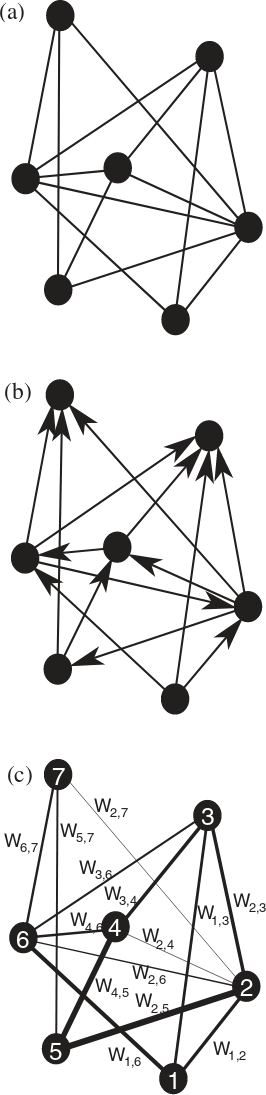
\includegraphics[width=\marginparwidth]{./Figures/intro/network_theory/graph_properties_Boccaletti2006.png}
%\captionof{figure}[Three types of graphs]{An undirected (a), a directed (b), and a weighted undirected (c) graph. From \cite{Boccaletti2006}}
%}
%}
%\end{scriptsize}

Starting with the building blocks of networks, we may define a \textbf{graph} as a pair of sets $G = (V,E)$, where $V = \{v_1,v_2,...,v_n\}$ is the set of \textbf{nodes} of the graph, and $E$ is the set of \textbf{edges}, or links, of the graph connecting pairs of nodes. The set $E$ can be any subset of all ordered pairs of $V$, such that $E \in V \otimes V$. Graphs can be either \textbf{directed} or \textbf{undirected} depeding on whether their constituent links are directional, i.e. whether $[v_i,v_j] \in E$ implies $[v_j,v_i] \in E$ (Fig. 1.1). Further, simple graphs are antirreflexive, meaning that a node cannot be linked to itself, i.e. $[v_i,v_j] \in E$ implies $i \neq j$.

Such a simple configuration can be easily extended by considering weighted or quantitative links. By incorporating weights, a \textbf{weighted graph} is a quadruple $G = (V,E,W,f)$, where $V$ and $E$ are the sets of nodes and edges defined above, $W = \{w_1,w_2,...,w_n\}$ is a set of weights such that $w_i \in \mathbb{R}$, and $f: E \rightarrow W$ is a mapping assigning weights to edges.

Intuitively, we say that two nodes $v_i$ and $v_j$ are \textbf{adjacent} to each other, or connected, if they are joined by an edge $e = \{v_i,v_j\}$. Similarly, two edges are adjacent if they are incident to at least one node.

The most basic structural property of a node is its \textbf{degree}. It is defined simply as the number of links incident to it. In directed graphs, one may distinguish in-degree, the number of links incident to a node, from out-degree, the number of links incident from it.

\begin{figure}[ht]
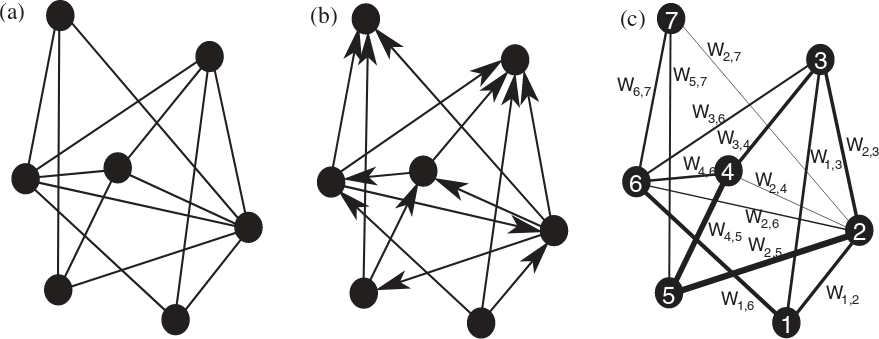
\includegraphics[width=\textwidth]{./Figures/intro/network_theory/graph_properties_Boccaletti2006_horizontal.png}
\caption[Three types of graphs]{An undirected (a), a directed (b), and a weighted undirected (c) graph. From \cite{Boccaletti2006}}
\label{fig:network_types}
\end{figure}

The \textbf{shortest path} connecting two nodes $v_i$ and $v_j$ is defined as the path with the shortest number of edges that connects them. This quantity, $L_{min}$, is also called the \textbf{distance} between two nodes. For weighted graphs, this definition may be refined to consider edge weight, such that the shortest path is the one that minimizes the summed weight of the edges connecting the two nodes.

A graph, in the context of network theory, is termed a \textbf{network}, and we will use this term hereafter. A network is said to be \textbf{complex} when it possesses topological features that are neither random nor completely regular. These features refer to properties of the network as a whole, and three of the most widely studied features of network are their degree distribution, their average path length and their clustering coefficient.

The \textbf{degree distribution} of a network is the probability distribution of the degrees of the network nodes. It is an important property of complex networks, as the degree distributions of random networks differs systematically from that of empirical networks of different types \citep{Barabasi1999}. While randomly assembled networks display Poisson degree distributions, many real networks are best represented as having power-law degree distributions. This means that in real networks, most nodes are typically connected to only a few other nodes (i.e. have a low degree), whereas a small number of nodes are highly connected. Networks with power-law degree distributions are alternatively called \textbf{scale-free networks} (Fig. \ref{fig:scale_free}).

\begin{figure}[ht]
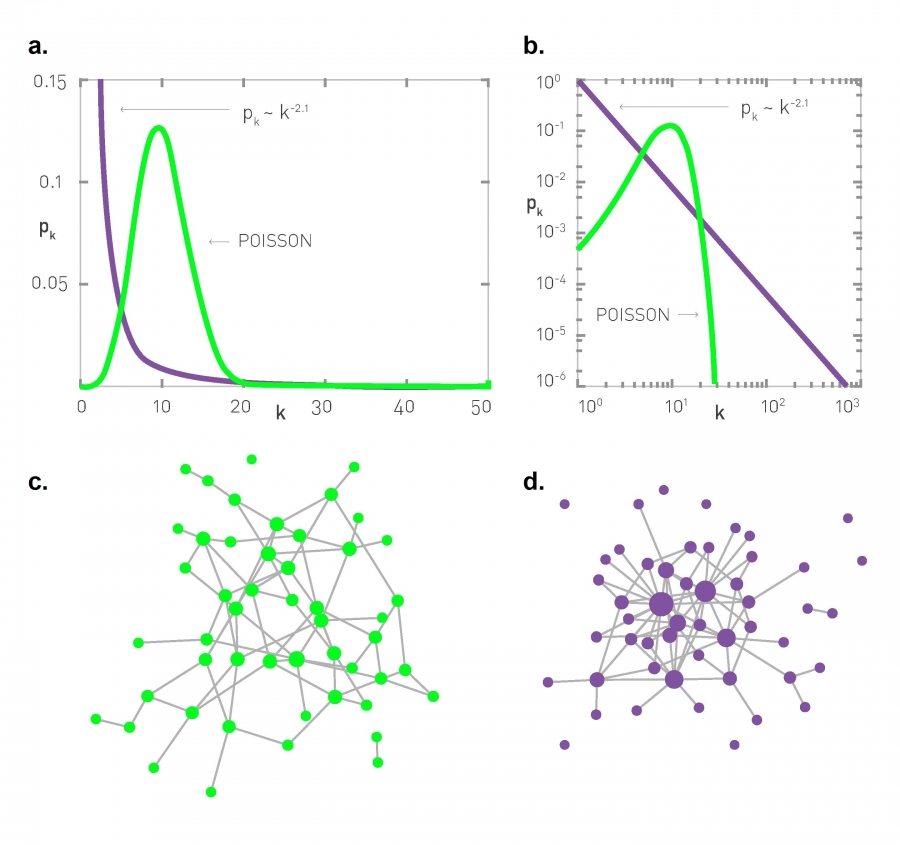
\includegraphics[width=\textwidth]{./Figures/intro/network_theory/degree_distrib_Barabasi2016.jpg}
\caption[Random and scale-free degree distributions]{\color{Gray} Degree distributions from random (green) and scale-free networks (purple) in natural (a) and logarithmic (b) axes. The hubs present in scale-free networks are evident in the network depiction (d). From \cite{Barabasi2016}}
\label{fig:scale_free}
\end{figure}

The \textbf{average path length} of a network is the average of the shortest paths between each pair of network nodes. It is given by

\begin{equation}
L = \frac{1}{S(S-1)} \sum_{i,j=1,S;i \neq j} L_{min}(i,j)
\end{equation}

and gives a measure of connectedness between any pair of nodes. Both random and scale-free networks display characteristically short average path lengths \citep{Montoya2002}.

Another important topological property is the \textbf{clustering coefficient}. It measures the degree to which the neighbours of a given node are linked together. Given a node $i$ with degree $d_i$, its local clustering coefficient is defined as

\begin{equation}
C_v(i) = \frac{2E_i}{k_i(k_i - 1)}
\end{equation}

where $E_i$ is the number of links between the $k_i$ neighbors of node $i$. The clustering coefficient of the network is the average over all $S$ nodes:

\begin{equation}
C_v = \frac{1}{S} \sum_{i=1}^{S} c_v(i)
\end{equation}

When considering network topology, networks without any differentiation between nodes, where each node can in principle interact with any other node, are called \textbf{unipartite}. Another common type of ecological networks is that which represents two disjoint groups that interact with each other but not with members of the same group (for example, a network with a group of plant species and a separate group of pollinators, Fig. \ref{fig:bipartite_nested}). Such networks are called \textbf{bipartite}.

\begin{figure}[ht]
\centering
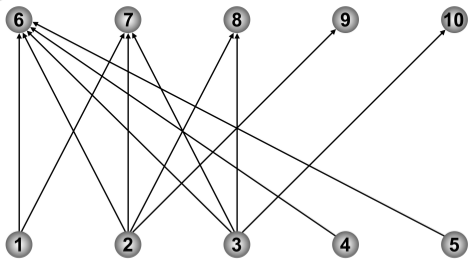
\includegraphics[width=0.5\textwidth]{./Figures/intro/network_theory/bipartite_nested_network_Ings2009.png}
\caption[Nested bipartite network]{\color{Gray} A bipartite network, in which nodes 1-5 and nodes 6-10 form sets that do not have within-group links. The network is also nested: the diet of consumer 8 is a subset of that of consumer 7, which in turn is a subset of that of consumer 6. From \cite{Ings2009}}
\label{fig:bipartite_nested}
\end{figure}

Several other network properties are widely used in the context of ecological networks. Here I will mention three of them. First, the \textbf{connectance} of a network is the proportion of realized links with respect to the potential number of links in the network. It is defined in different ways depending on the assumptions about the feasible links of the network. Four variations are possible regarding the directedness of the network and the feasibility of self-loops. The most general case is a directed network where self-loops are allowed. In that case, the set of potential links is simply $L_p = S^2$ for a network of $S$ nodes. If self-loops are not allowed, the set of potential links is $L_p = S^2 - S$, whereas if the network is undirected, the number of potential links halves, i.e. $L_p = S^2/2$. Therefore, an undirected network with no self-loops has $L_p = (S^2 - S)/2$ potential links. The general definition of connectance is

\begin{equation}
C = \frac{L}{L_p}
\end{equation}

where $L$ is the number of realized links.

The above definitions of the set of potential links imply that, aside from the consideration of self-loops, all links between any pair of species are potentially feasible.

Another topological property widely studied, \textbf{modularity} is the tendency of the network to display modules highly connected within but largely disconnected from each other. The detection of modules, or clusters, in networks is an active area of research, and a closed definition of modularity depends on the expected number of modules and their link distribution. As an example, \cite{Fortuna2010} defined modularity as

\begin{equation}
M = \sum_{s = 1}^{N_M} \left[\frac{l_s}{L} - \left(\frac{d_s}{2L}\right)^2\right]
\end{equation}

Lastly, \textbf{nestedness} is a property of bipartite networks by which nodes with low degree are connected to a subset of the nodes linked by nodes with high degree (Fig. \ref{fig:bipartite_nested}).

Aside from these general definitions, it is important to mention the matrix representation of networks. Intuitively, by defining a matrix $A$ of dimensions $S * S$, its entries $a_{i,j}$ may represent the existence (or weight) of a link between nodes $i$ and $j$. Such matrix is called the \textbf{adjacency matrix}. If the network is undirected, its adjacency matrix is symmetric, i.e. $a_{i,j} = a_{j,i}$

\[
A_{undirected} = \begin{pmatrix}
0& 1& 0 \\
1& 0& 1 \\
0& 1& 0
\end{pmatrix}
\]

where $a_{i,j} = 1$ if a link exists between nodes $i$ and $j$, and $a_{i,j} = 0$ otherwise. If the network is directed, the possibility exists that $a_{i,j} \neq a_{j,i}$, so that an example matrix can be

\[
A_{directed} = \begin{pmatrix}
0& 1& 0 \\
0& 0& 0 \\
1& 1& 0
\end{pmatrix}
\]

The convention for directed networks is that adjacency matrices represent the interaction originating in column $j$ and affecting row $i$, so that in the previous example, there is a link from node 2 to node 1, but not the other way around. %The matrix formulation of networks has particular importance in evaluating the stability properties of the associated system, and thus has been extensively used in studies of ecological dynamics. In the next section, I briefly review early developments on ecological networks and further develop some of the properties defined above.

\subsection{Ecological networks: brief history, recent developments and open questions}

The general definitions outlined above can be applied to ecological systems seamlessly by defining individuals, species or guilds as nodes, and the biotic interactions among them as the edges or links connecting them. Indeed, natural historians and early ecologists had recognized the network nature of ecological communities long before the recent developments on complex networks. The brief historical review that follows draws primarily from the works by \cite{Bersier2007} and \cite{Ings2018}, and the reader is referred to these studies for consulting primary references.

The first documented observations about the interactions of species can be traced back to Ancient Greece, where mutualistic relationships were observed by Herodotus, Theophrastus and Aristotle. In turn, the arab scholar Al-Jahiz is believed to have introduced the concept of food chain in his \textit{Book of the Animals}, in the 9th-century. In the early Enlightenment the documented study of the natural world began to gain back attention, although admittedly on a secondary position with respect to mathematics, physics, chemistry or astronomy, disciplines that constituted the main focus of the Scientific Revolution. Observations about empirical food chains are documented by van Leeuwenhoek and Linnaeus, but it would be Alexander von Humboldt in the 19th-century, throughout all his works, the first and most influential proponent of a view of nature that emphasized the complex web of relationships between species, looking at nature as a ``living whole''. The first representation of a full network of trophic interactions dates from 1880, and was made by the italian scientist Lorenzo Camerano.

After these and other seminal contributions, the 20th-century saw the confirmation of network-oriented approaches to ecological issues. The ecologist Charles Elton developed many important concepts, such as the ``pyramid of numbers'' by which abundances decreased along the food chain, and established the terms \textit{food chain} and \textit{food cycle}. After his seminal works, the network representation of trophic relationships became a common framework for studying ecological communities. By this point, trophic relationships were already the most studied interactions in ecological communities. Trophic interactions are ubiquitous in nature, they are usually the easiest to document and, unlike other interactions, can be used to outline the fluxes of biomass and energy in a given community. It is, therefore, not surprising that they took, and still maintain, such a predominant role in studies of ecological networks. The figure of Raymond Lindeman also stands out in the first half of the 20th century, with his work ``The trophic dynamic aspect of ecology'', in which he studied for the first time the quantitative fluxes and feedbacks between the biotic and abiotic components of an entire ecosystem, the Cedar Bog Lake in Minnesota \citep{Lindeman1942}. As \cite{Ings2018} note, limnology had a prominent position on these early developments, and many temperate lakes were the first ecosystems to be thoroughly sampled and studied.

In parallel to these insights from natural systems, the mathematical foundations for studying the dynamics of ecological interactions were being developed. The mathematician Alfred J. Lotka proposed in 1920 a set of equations for the population dynamics of a pair of predator and prey species, that explained the apparent oscillations observed in plant-herbivore systems \citep{Lotka1920}. In an independent contribution another mathematician, Vito Volterra, derived similar equations following observations of fish catches in the Adriatic Sea \citep{Volterra1928}. The general form of these equations is

\begin{equation}
\begin{array}{c}
\frac{dx}{dt} = \alpha x - \beta xy \\
\frac{dy}{dt} = \delta xy - \gamma y
\end{array}\label{eq:LV}
\end{equation}

where $x$ is the number of prey, $y$ is the number of predators, $\alpha$ is the growth rate of the prey, $\beta$ the predation rate coefficient, $\delta$ the predator's growth rate, and $\gamma$ its mortality rate. In this model, both species modulate their abundances in response to the other (Fig. \ref{fig:LV_example}), and the non-trivial solution to the system, formulated as with eq. \ref{eq:LV} is stable and periodic. The Lotka-Volterra set of equations implies a series of assumptions about the underlying biological system. First, they are an example of a mean-field system, thus assuming an homogeneous habitat in which individuals are interacting without constraints or variations. Prey populations in the absence of the predator display exponential growth (i.e., if $ y = 0$, the variation in prey density is given by $\alpha x$), and the predator depends entirely on the prey population. Furthermore, predators do not satiate, in that they respond instantaneously to increases in prey population. Importantly, all $\alpha , \beta , \delta , \gamma$ coefficients are constant, thus assuming no other sources of variation.

\begin{figure}[ht]
\centering
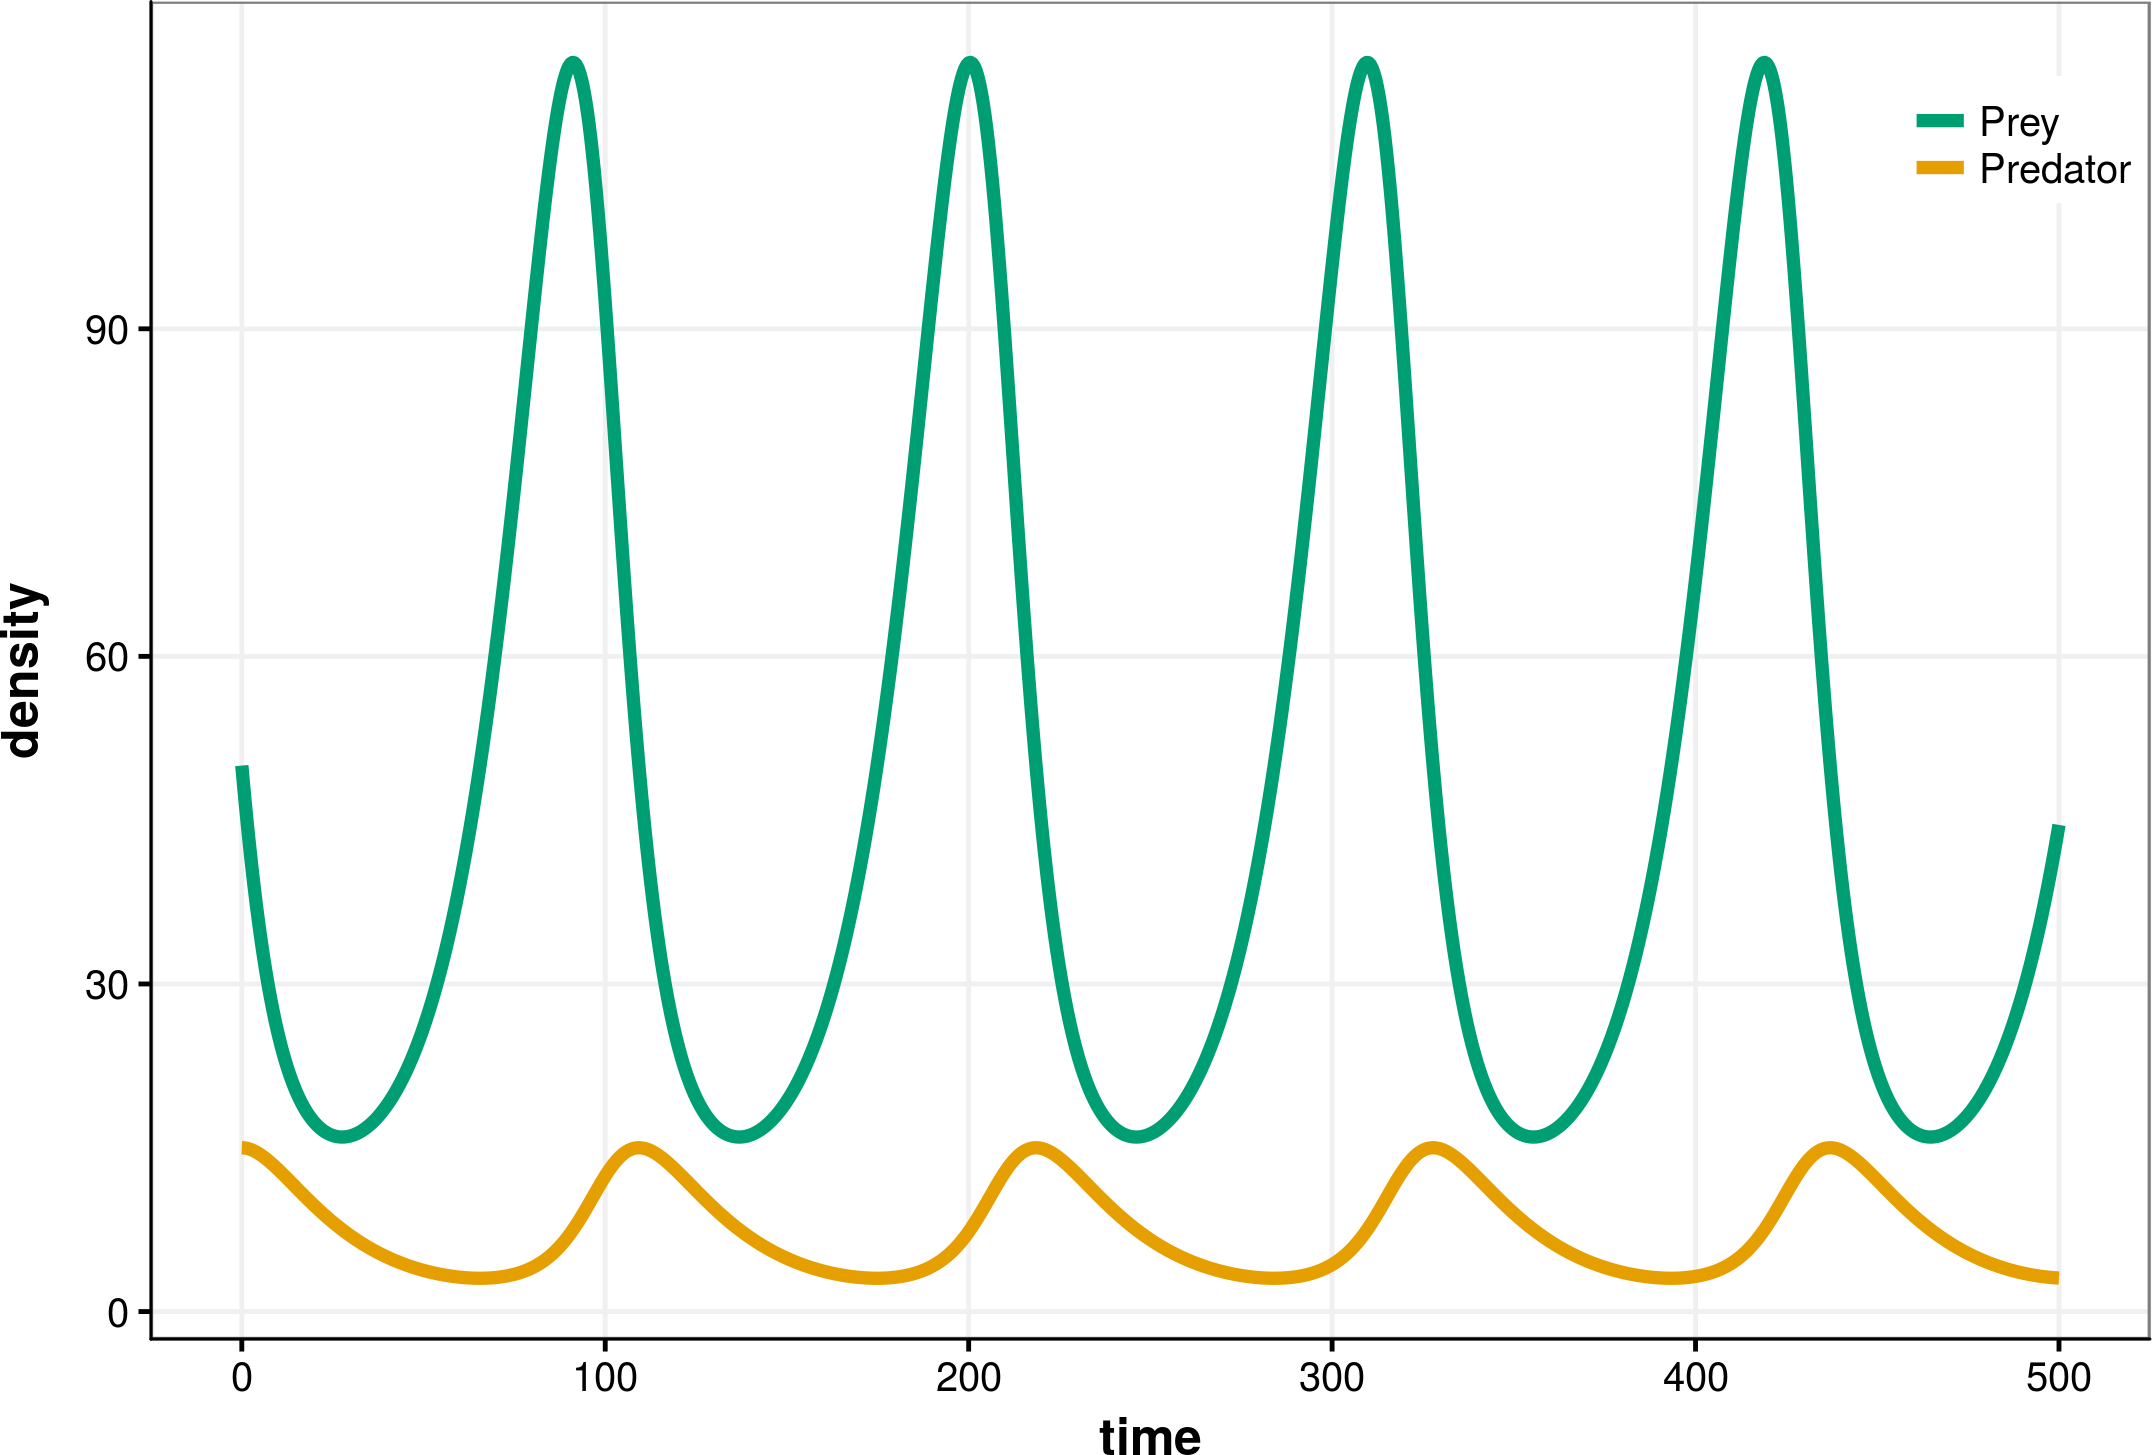
\includegraphics[width=.6\textwidth]{./Figures/intro/ecological_networks/LV_example.png}
\caption[2-species Lotka-Volterra system]{\color{Gray} Lotka-Volterra equations generate stable population dynamics in which densities of the prey and the predator species are both dependent on each other.}
\label{fig:LV_example}
\end{figure}

In the context of dynamical systems, the stability of the system can be approached by analysing how the system responds to very small perturbations off a steady state. This is done by calculating the \textit{eigenvalues} of the system, values that encapsulate the response of the system to such a small perturbation around the equilibrium. The mathematics behind the calculation and interpretation of eigenvalues have been thoroughly developed, and the interested reader may find innumerable derivations of it. In the context of ecological networks, the book \textit{Food Webs} by Kevin \cite{McCann2011} gives a well-balanced introduction to the study of dynamical systems. The important message is that the eigenvalues of a dynamical system (in particular, the maximum eigenvalue) are informative about the stability of the system. Positive eigenvalues will imply that the system is locally unstable, whereas negative eigenvalues mean that the system is locally stable around that particular equilibrium.

Despite the initial insights from 2-species model systems, many ecologists were, as we have seen, much more interested on the notion of stability of whole communities or ecosystems. The first conceptual treatments of community stability can be traced back to Eugene Odum, who suggested that in a community, the number of alternative paths a quantum of energy has for going from primary producers to top predators is a measure of the stability of the community. This notion that the more links an ecological network had, the more stable it was (or, in other words, that ``complexity begets stability''), was the prevalent opinion up until the early 70s. Robert MacArthur, in another highly influential study, analyzed the stability of complete food webs in a semi-quantitative way. He arrived to the hypothesis that community stability increases by either increasing the number of species in a community, or the connectance of the associated food web \citep{MacArthur1955}.

The complexity-stability dichotomy of ecological communities entered a new dimension after the seminal work of Robert May \citep{May1972}, who used for the first time mathematical models of idealized communities to assess the local stability of systems with an indeterminate number of species modelled with Lotka-Volterra dynamics. He found that, in randomly assembled networks with normally distributed interaction strengths, the dynamical systems remain locally stable if

\begin{equation}
\alpha \sqrt{SC} < 1\label{eq:May}
\end{equation}

where $\alpha$ is the average interaction strength, $S$ is the number of species, and $C$ is the connectance of the network in the form $L/S^2$. The interpretation is that an increase in either mean interaction strength of the system, species richness, or number of links, would rapidly tend to destabilize the system. Crucially, May was of course aware of the limitations of his approach: the assembled networks possessed no structure whatsoever, pairwise interaction strength was assumed to be a constant, stochastic parameter, and the definition of stability involved infinitesimally small perturbations from an equilibrium state, as given by the eigenvalues of the system. Nevertheless, regardless such obvious limitations, May's work was the first quantitative derivation about the expected stability of arbitrarily large ecological communities, and not only so, but it also was a frontal attack on the common wisdom championed by MacArthur (who passed away way too early, in 1972) and many others by that time. The debates and number of studies triggered by May's results are countless, both in the camps of the theoreticians and the empiricists. From that moment onwards, the study of ecological networks started to gain even more attention and took many different parallel paths. An important line of research, that did not start with May's results but definitely gained attention after them, follows the estimation of interaction strengths both in theoretical studies of functional responses \citep{Holling1965} and empirical estimations \citep{Bender1984}.

Robert Paine showed in 1966 that the effects of removing a top predator could propagate throughout the whole ecological network, eventually altering the richness of the community \citep{Paine1966}. This striking result led to the denomination of \textit{keystone species} to those species with a disproportionate influence in the overall structure and dynamics of the community. He continued to be interested in measuring the impacts of one species over another and on the overall community, a theme that came together with the theoretical importance of interaction strength proposed by May. Theoretical metrics of interaction strength represent changes in different per capita or population-level parameters \citep{Laska1998} but such metrics are, importantly, not generally equivalent to what is measured in experimental studies (e.g. \citealt{Bender1984}). Paine observed that descriptions of food webs that failed to account for estimates of interaction strengths were not enough in order to link the structure of food webs with their dynamical behaviour \citep{Paine1992}.

However, obtaining empirical estimates of all interaction strengths in a given network is so far unfeasible even for moderately rich communities, given the complexity of the combinations and feedbacks of effects between the different species involved. This divide between theoretical models and empirical estimates of interaction strengths is still one of the main unresolved problems in network ecology. Theoretically, it has been shown that, within the framework of local stability analyses and for networks considering only trophic interactions, stability is enhanced when a majority of interactions are comparatively weak and only a few are comparatively strong \citep{McCann1998,Berlow1999}. Incidentally, a recent article showed this pattern to hold in a set of empirical food webs \citep{Jacquet2016}.

Aside from the studies on theoretical and empirical interaction strength, and its importance on community stability, another strong source of discussion arising from May's results is the role that non-random structural patterns played in conferring stability to empirical networks. The first empirical food webs to be collected and analysed for structural regularities approach in the late 70s, in particular in a seminal book by Joel \cite{Cohen1978}. An early focus of studies on food web structure was the role of \textit{connectance}, given its relationship to theoretical stability (eqn. \ref{eq:May}). Early efforts tested, for example, the potential invariance of the relationship between number of links and number of species $L/S$, as a means of corroborating May's criterion (see \citealt{Pascual2006} for details).

The early compilations of empirical food webs, however, were not even close to be complete descriptions of their systems, and had important flaws such as differential level of node taxonomic aggregation. Newly collected data in the early 1990s \citep{Polis1991, Martinez1991} showed that network metrics and relationships outlined with earlier food webs were in many cases artifacts of the poorly collected data \citep{Pascual2006}, and this realisation triggered a reorientation of efforts and development of new hypotheses and ideas concerning food web structure. Among them, an important theoretical model of food web structure, the niche model \citep{Williams2000}, proved able to generate food webs with realistic structural patterns out of a single niche axis in which all consumer species are sorted. More recently, species-level traits and their distribution have proven to be important in characterizing food web structure, as shown for example by \cite{Laigle2018}.

In parallel to these more recent developments on food webs, studies on other types of interactions started to emerge in the late 20th century. The first attempt at characterizing a network of positive interactions was made by Pedro \citet{Jordano1987}, who studied patterns of connectance and interaction strength in plant-pollinator and plant-seed disperser networks. From his seminal study, a whole field of research opened up, and the study of bipartite mutualistic networks has produced many insights regarding the structure and dynamics of these communities \citep{Vazquez2009a, Bascompte2013}. In particular, bipartite mutualistic networks have been shown to be generally nested, and this nestedness is an important feature for their stability, as opposed to food webs, which are thought to be comparatively less nested and more modular \citep{Thebault2010}.

It is now sufficiently clear that, in any case, mutualistic interactions are structured in a non-random fashion in empirical bipartite networks, and this structure has important consequences for their dynamics. Regarding the study of interaction strengths in mutualistic networks, the functional responses of mutualism are much less studied than those of predator-prey interactions \citep{Holland2002}, and a novel line of research focused on estimating the net impact of a species over another by using as a surrogate their interaction frequency \citep{Vazquez2005}. This approximation is likely dependent on the specific type of mutualism considered. For example, in a study analysing plant-hummingbird networks, \cite{Vizentin-Bugoni2014} showed that trait-matching was more important for structuring these ecological networks than abundances alone. In further studies, interaction frequency itself has been found to be well approximated by the abundances of the interacting species \citep{Vazquez2007}. This methodology for estimating population-level short-term impacts is thus promising for mutualistic networks in which no other quantitative effects are available. Importantly, the approximation hinges on interactions being stochastic, with no trait-mediated selection of interaction partner or frequency. In that sense, it may also serve as a baseline against which to compare the effect of traits in specifying interactions \citep{Poisot2015}.

All in all, the knowledge about the structure and dynamics of single-interaction ecological networks has increased enormously in the last few decades. A fundamental question that we may ask is the extent to which these varied insights are applicable to empirical, complex communities. Despite the convenient distinction between interaction types commonly made for studying ecological networks, communities are composed of individuals interacting in many different ways, with varying intensities and at different spatial and temporal scales.

We know now that, at the very least, both predator-prey and mutualistic interactions are highly structured in empirical communities. We lack, however, a general framework for ecological networks in which different interaction types are integrated, and where the combined structure of the network can be analysed. This integration, of course, will have important implications for community dynamics: for example, including non-trophic interactions onto food webs has already been shown to importantly alter their stability patterns \citep{Kefi2012, Kefi2016a}, or their robustness to secondary extinctions \citep{Pocock2012}. This change of scope about ecological communities may also trigger novel questions about their structure and dynamics. It may seem surprising on a first look, but we currently do not know how the different interaction types are distributed in empirical communities generally. Actually, given the difficulty of compiling different interaction types in a systematic way for any relatively rich community, it becomes clear that approaching such a fundamental question requires important observational and experimental efforts. In that sense, a general theoretical framework for multiple interactions networks may help develop targeted hypothesis about empirical communities, from which to build observational or experimental studies. Related important questions concern the role of spatial patterns or environmental gradients in shaping the combined structure of ecological networks. For example, does the spatial structure of the different interaction types vary? How does this influence the spatial propagation of effects? Does the relative importance of the different interaction types vary across environmental gradients?

In single-interaction networks, the role of space in shaping their structure and stability has been recognised as a key factor, e.g. by analysing how different communities are connected by dispersal and the implications for the overall metacommunity \citep{Leibold2004}, or how network structure varies with spatial scale \citep{Galiana2018}.

In order to integrate recent advances on multiple interactions networks with the spatially explicit framework of metacommunity ecology, some issues need to be resolved before a proper multiple interaction metacommunity framework is developed. For example, what is the nature of the connections between spatially separated communities? Mobile species are capable of displacements in order to look for food sources (antagonism, mutualism), or in order to establish themselves in another territory (dispersal). It is important to know if there is a relationship between the movement capacity of a given species and its tendency to engage in different interaction types. It is also important to develop theory on the spatial propagation of interaction effects: how do the different types of interaction propagate in space? Are some interaction types more likely to have a greater impact on the overall community than others? Or is the effect only related to the relative magnitude of the interaction, and the centrality of the species involved?

Some of these questions have been barely explored even in metacommunities of single interaction types. Most metacommunity studies follow the long-standing history of horizontal communities and consider how competitive guilds are connected in space, and only recently is metacommunity theory being expanded to account for mulitrophic networks \citep{McCann2005, Fahimipour2014, Gravel2016a}. It is therefore necessary to strenghten the foundations of metacommunity theory before integrating it with the paradigm of multiple interactions networks.

From a more general point of view, one can also ask whether the structure and dynamics of ecological networks vary across different types of gradients, and if so, what are the factors and processes driving this variability. The variability of ecological interactions across environmental gradients has been studied under different subfields of community ecology, from the point of view of horizontal communities (mainly plants: the Stress Gradient Theory, see e.g. \citealt{Maestre2009}) and theoretical food webs with competitive interactions (Environmental Stress Models, see \citealt{Menge1987}). Stress Gradient Theory focuses on evaluating the response of communities to variations in environmental stress, and does so by studying plant communities which, as stated by theory and empirical observations, may exhibit variations in the relative importance of competitive versus facilitative interactions as stress increases \citep{Callaway1997}. This theory, however, is currently not applicable to multitrophic communities, despite recent attempts to test its validity for higher trophic levels \citep{Barrio2013}. Environmental Stress Models, in turn, were developed to predict the differential role of top-down and bottom-up processes in food webs across gradients of environmental stress. While theoretically comprehensive, their difficulty of testing has prevented further developments except for localised, targeted systems (e.g. \citealt{Cheng2016a, Daleo2015}). In any case, none of these theories incorporates the whole array of interactions potentially occurring in nature, and a further issue is that the different types of environmental gradient that mediate ecological processes are usually taken together, without differentiating the different environmental components that may affect interactions and demographic processes. Therefore, we are still far from a general theory on ecological networks and their variability across environmental gradients.

\section{Objectives}

In my thesis I addressed fundamental unresolved questions about ecological networks in general. Chapters 2 and 3 deal explicitly with networks of multiple interaction types, and the rest of the thesis explores fundamental questions for which more simple model systems are used, in order to focus on the specific questions at hand before adding the complexity of multiple interactions. The following general objectives constitute the main chapters of the thesis:

\begin{itemize}
\item \textbf{To review and synthethise current methodologies for modelling multiple interactions in ecology}\\ \\
First, I aimed to synthesize and organize the growing literature on this type of networks, while at the same time laying down some methodological foundations for future theoretical studies on the subject.

\item \textbf{To understand how the frequency and distribution of the different interactions drive species persistence}\\ \\
Second, I developed a general theoretical model in which I tackle several key issues about network structure and dynamics. I aimed at deriving general hypotheses about the persistence of species in complex networks with realistic structural patterns.

\item \textbf{To know how Species Abundance Distributions are influenced by the structure of multitrophic communities}\\ \\
Third, I looked at a classic pattern from horizontal community ecology, the Species Abundance Distribution, from a network perspective. In order to understand how the frequency and/or distribution of interaction types influences the distribution of abundances in a given community, first it is necessary to develop theoretical expectations about its distribution on more simple networks, for example food webs. I drew from the extensive literature on food webs and trophic relationships in general to derive basic hypothesis about the variation of Species Abundance Distributions across trophic guilds.

\item \textbf{To advance in the understanding of interaction effects in space}\\ \\
Fourth, I studied the role of space in propagating interaction effects. As with the previous chapters, no general hypotheses exist about the spatial propagation of interaction impacts, so in order to provide baseline expectations and for our study to be comparable to previous efforts, I focused on the effect of trophic interactions and how they propagate when species disperse or forage in a set of spatially connected communities.

\item \textbf{To explore whether environmental factors drive the frequency of different types of interactions}\\ \\
Fifth, I studied how interactions are likely to vary across environmental gradients. This issue has been explored independently in different subfields of community ecology, but the conclusions obtained have been largely overlooked in other fields. I recovered the classic differentiation in environmental factors first proposed by Hutchinson and delve in how gradients in different types of environmental factors may drive variations in the prevalence of different interaction types and other community properties. Given the paucity of studies and theory in this question, I took the same approximation as in chapters four and five, and resorted to basic horizontal communities, in order to provide general foundations from which ideas about more complex communities can be developed.

\end{itemize}

%************************************************
\chapter[Multiple Interactions Networks]{Multiple interactions networks: towards more realistic
descriptions of the web of life}\label{ch:review}
%************************************************

%\tikz[remember picture,overlay] \node[opacity=0.3,inner sep=0pt] at (current page.center){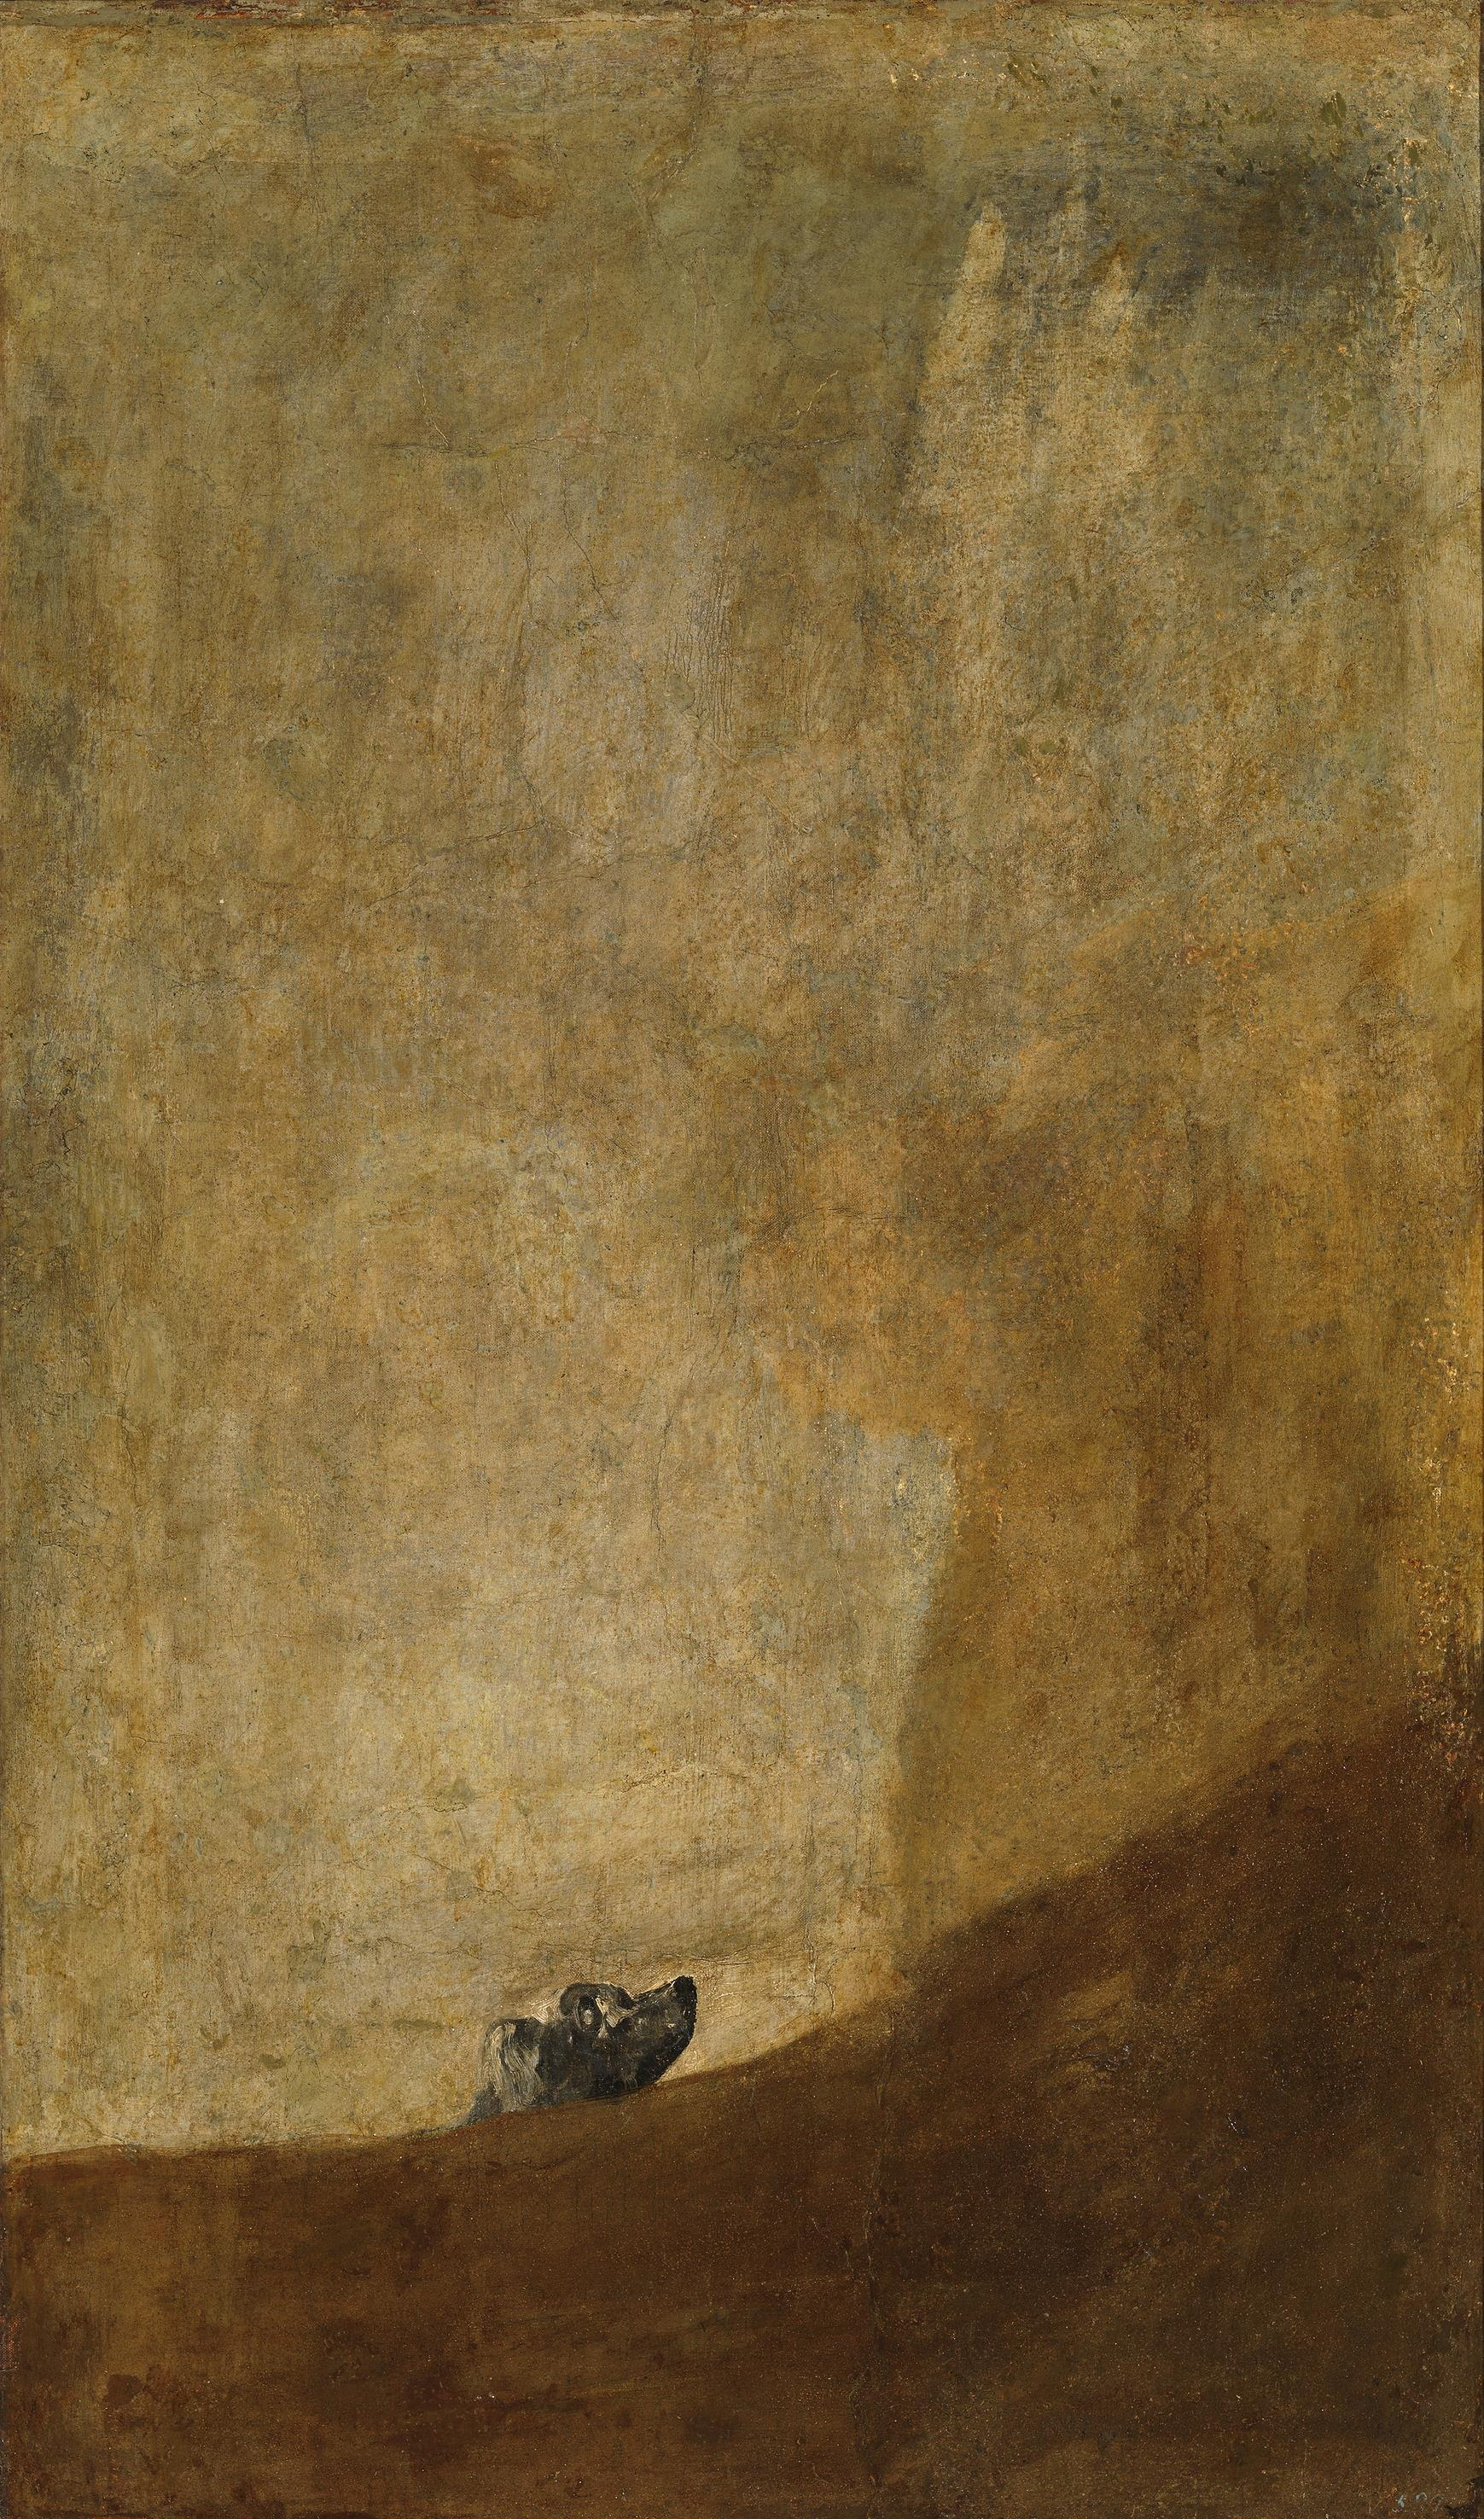
\includegraphics[width=\paperwidth,height=\paperheight]{./Figures/cover/Goya_Dog.jpg}};
\tikz[remember picture,overlay] \node[opacity=0.3,inner sep=0pt] at ([yshift=3cm,xshift=2cm]current page.center){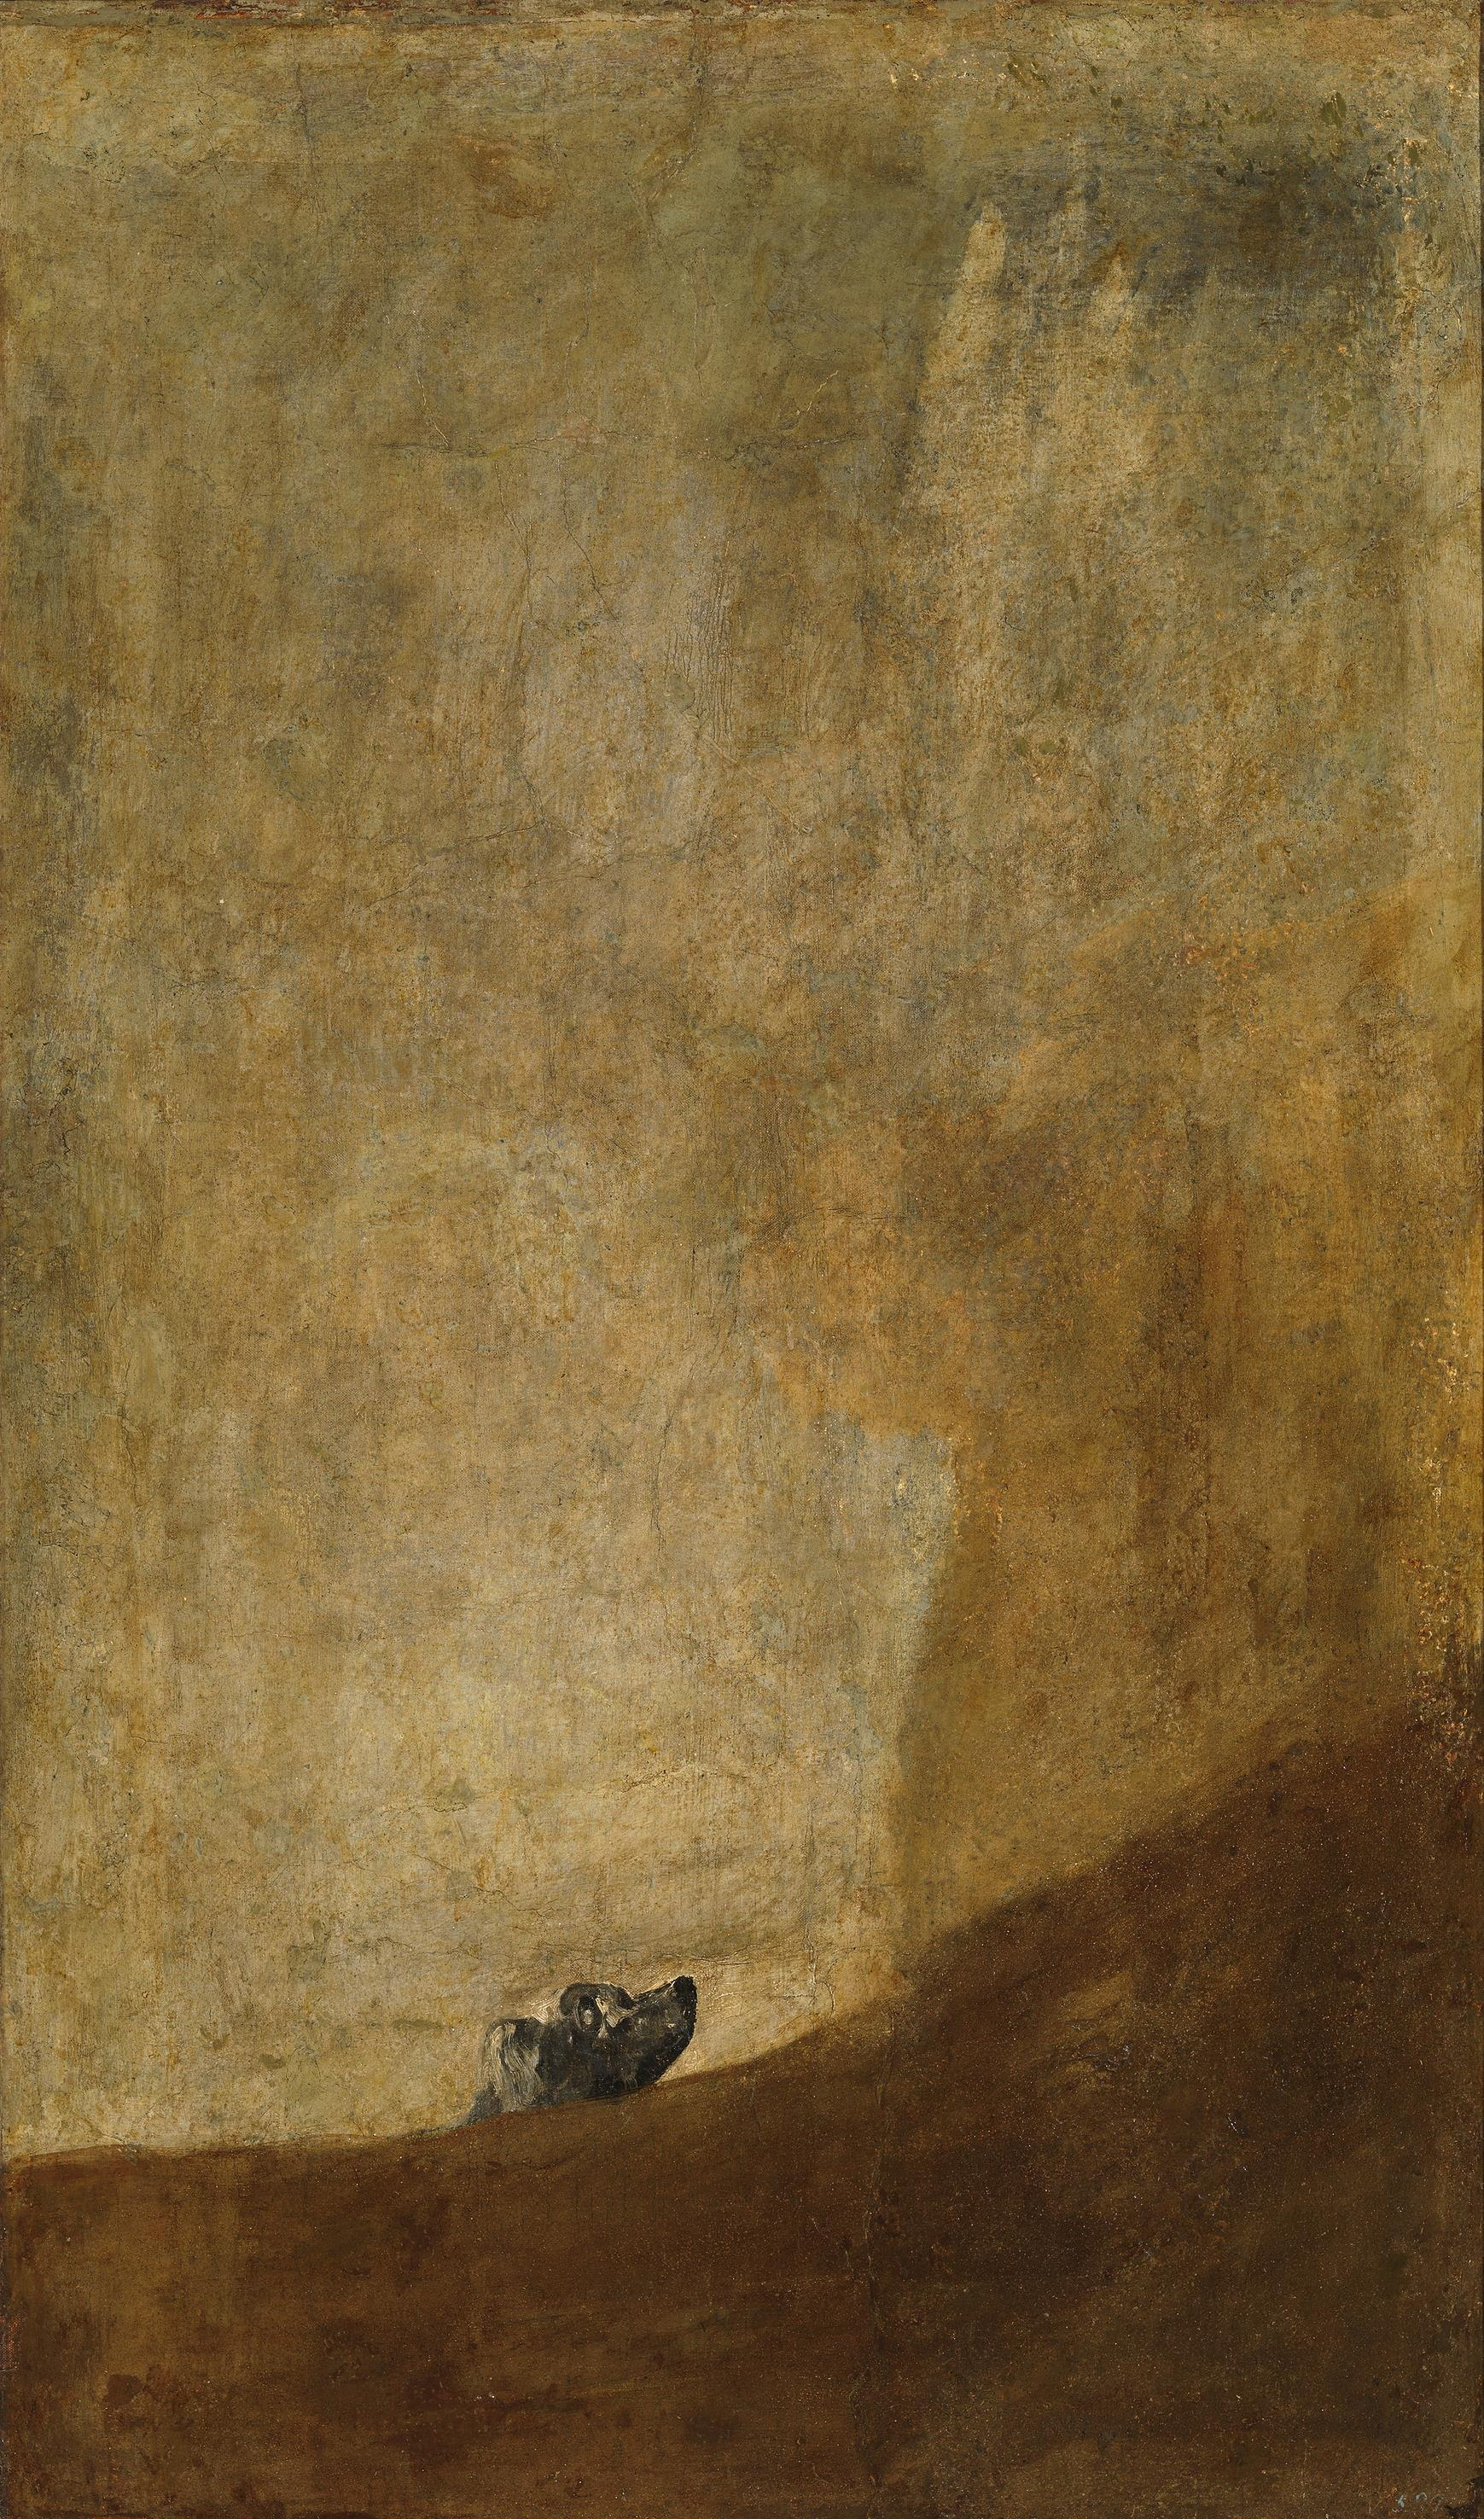
\includegraphics[width=\paperwidth,height=\paperheight]{./Figures/cover/Goya_Dog.jpg}};
\clearpage

\section*{Abstract}
Ecological communities are defined by species interacting dynamically in a given location at a given time, and can be conveniently represented as networks of interactions. Pairwise interactions can be ascribed to one of five main types, depending on their outcome for the species involved: amensalism, antagonism (including predation, parasitism and
disease), commensalism, competition or mutualism. While most studies have dealt so far with networks involving one single type of interaction at a time, often focusing on a specific clade and/or guild, recent studies are being developed that consider networks with more than one interaction type and across several levels of biological organisation. We review these developments and suggest that three main frameworks are in use to investigate the properties of multiple interactions networks: ‘expanded food-webs’, ‘multilayer networks’ and ‘equal footing networks’. They differ on how interactions are classified and implemented in mathematical models, and on whether the effect of different interaction types is expressed in the same units. We analyse the mathematical and ecological assumptions of these three approaches, and identify some of the questions that can be addressed with each one of them. Since the overwhelming majority of studies on multiple interactions are theoretical and use artificially generated data, we also provide recommendations for the incorporation of field data in such studies.

\section{Community ecology and network theory}
Ecological communities should be defined not only by lists of co-occurring species, but also by the myriad of interactions taking place among them. A convenient way to include information about both species composition and their interactions is to represent communities as networks in which species are nodes connected by links representing biotic interactions. Network analyses can provide insights into community local stability \citep{Allesina2012} and robustness to extinctions \citep{Riede2011a}, the degree of specialization of individual species or guilds \citep{Dorado2011}, the impact of invasive species or climate change on established communities \citep{Lopezaraiza-Mikel2007} and, more generally, on any question in which pairwise interactions relate to community patterns and processes.

Networks can accommodate different types of data, depending on the nature of the links between species (e.g., qualitative, quantitative, static, dynamic), the temporal and spatial resolution of the community, the level of aggregation of the nodes (e.g., individuals, species, trophic guilds), or the specific objectives of the study. A common simplification is to study networks of a single interaction type, e.g., trophic \citep{McCann2011} or mutualistic \citep{Bascompte2013}, assuming (often implicitly) that the effect of other interactions on community dynamics is negligible compared to the ones analysed. Such an assumption is usually unavoidable given the lack of comparable data on different interaction types, but it is becoming increasingly clear that the effects of interactions not accounted for in analyses of single-interaction networks (including indirect ones; but see \citealt{Cazelles2016}) might be significant for species persistence \citep{Soliveres2015a, Kefi2016a} and community structure \citep{Sander2015, Golubski2016}. Furthermore, analyses of interaction networks of a single type often yield differential results regarding the factors that drive their stability. For example, among the factors reported to stabilize food webs are high modularity and low connectance \citep{Thebault2010}, correlation in pairwise interaction strengths \citep{Tang2014}, trophic coherence \citep{Johnson2014}, a preponderance of weak \citep{McCann1998} and asymmetrical interactions \citep{Bascompte2006}, degree distributions broader than those of random graphs \citep{Allesina2015}, or the appearance of generalist consumers coupling resources with different interaction strengths \citep{Rip2010}. On the other hand, mutualistic networks are thought to be more stable when highly nested and connected \citep{Thebault2010, Lever2014}, when there are demographic responses to interactions \citep{Lee2015}, or when mutualistic interactions are relatively strong \citep{Rohr2014}. The persistence and resilience of communities defined with multiple interaction types, however, will additionally likely be influenced at least by (1) the proportion of the different interaction types, (2) the relative strength of pairwise interactions both within and among interaction types, and (3) the structural properties of each sub-network and the overall aggregated network.

The study of single-interaction networks in ecology has progressed enormously in the last decades, both theoretically and empirically. In parallel, the analysis of multiple interactions networks has also advanced in other fields of study \citep{Boccaletti2014}. This novel paradigm has only recently started to be applied to ecological studies, with several examples of new conceptual developments being forged together with applications of old concepts to new problems (Table \ref{tab:table1.1}). Despite the relatively small number of studies using multiple interactions networks in ecology, the research objectives and methodologies that have been addressed are extremely diverse, and a synthesis of recent developments is timely. Here, we identify three main approaches for the design and analysis of ecological multiple interactions networks. These approaches have been used in theoretical and empirical studies without an explicit recognition of their conceptual underpinnings. We define them explicitly, examine their underlying ecological assumptions, the type of questions best addressed with each approach, and provide recommendations for the integration of empirical data.

\section{Multiple interactions networks in ecology}
Probably, the first study of ecological networks explicitly considering different interaction types was the classic study by \cite{May1972}, in which he assembled interaction matrices with random coefficients from a Gaussian distribution  $N{\sim}\left(0,\sigma \right)$  , thereby allowing for negative and positive pairwise interactions to be considered. May's results showed that in theoretical communities assembled randomly, complexity (measured as connectance and species richness) was inversely related to the local stability of the system. But natural communities are highly complex, diverse and, nonetheless, seem to persist. After that seminal study, there has been a flurry of studies trying to uncover the processes and structural patterns that confer stability to empirical communities (e.g. \citealt{Saint-Beat2015}). However, comparable data on different interaction types is extremely difficult to acquire, and the focus for most of the second half of the 20th century has been on how competitive and antagonistic interactions drive population and community patterns (e.g. \citealt{Connell1961, Paine1966}). As predator-prey interactions are easiest to observe and document in the field, the analysis of empirical networks relied almost entirely on food webs for a few decades. Pioneering works by \cite{Jordano1987}, or \cite{Fonseca1996}, amongst others, paved the way for the study of mutualistic networks, but the first studies considering more than one interaction type in the same network only appeared in the last decade (Table \ref{tab:table1.1}).

Developing a theoretical framework for multiple interactions networks involves the integration of a variety of interaction types and effects, direct and indirect, taking place at different temporal and spatial scales. In this review, we propose two main criteria for classifying such frameworks. The first is the classification system applied to interactions \citep{Abrams1987}. Interactions can be defined based on the effect they produce on each member or, alternatively, on the mechanism by which the interaction is produced. Regarding effects, each interactor can be affected positively, negatively, or not affected at all by a pairwise interaction, regardless of the actual mechanisms by which the effect occurs. For example, a (-,-) interaction, defined as competition, could actually be realized through mechanisms as different as territorial, chemical or consumptive competition \citep{Schoener1983}. By defining all interactions with respect to the effect on each member (0,-,+), every effect-based classification is complete, in the sense that no interaction, however idiosyncratic, is left unclassified. Regarding mechanisms, interactions are defined according to the mechanism by which they take place, regardless of the effect on the interacting species. Thus, consumptive competition would be defined as an interaction in which each member is affected by consumption of a common limited set of resources, territorial competition would represent limitations on the available space for each interactor, and so on. A virtually unlimited number of interaction categories can be theoretically defined under this scheme, depending on the questions addressed.

The second criterion distinguishes network analyses based on whether the strengths of different interaction types have common units (i.e., their effects are comparable, acting upon the same population property) or not. This criterion only applies to classification schemes based on effects as, by definition, strengths of interactions acting explicitly through different mechanisms have different units, and are thus not amenable to being homogenized. For example, chemical competition between two plant species may be reflected on the mortality rates of the interacting populations, while a mutualistic interaction between a plant species and a seed disperser bird may affect the dispersal rate of the plant and the population growth rate of the bird. In an effect-based classification with the same units for every interaction, on the contrary, these and every other interaction could be taken to affect a single property (e.g. long-term population size), and hence would be comparable. Based on the two criteria proposed here, we distinguish three conceptual frameworks, already found in the literature, to construct and analyse multiple interactions networks: expanded food webs, multilayer networks, and equal footing networks (Fig. \ref{fig:fig2.1}).

%\afterpage{
%\clearpage% Flush earlier floats (otherwise order might not be correct)
%\thispagestyle{empty}% empty page style (?)
\begin{landscape}% Landscape page
\begin{footnotesize}
%\begin{longtable}{p{1.5cm}p{1.5cm}p{2cm}p{2cm}p{1.5cm}p{2cm}p{4cm}}
\begin{longtable}{p{1.5cm}p{1.5cm}p{2cm}p{2cm}p{2cm}p{2cm}p{4cm}}
\caption[Studies of multiple interactions networks]{\color{Gray}Studies considering networks of more than one interaction type. Analyses of small network modules ({\textless}5 species) are not included\label{tab:table1.1}}\\\hline
Study & Framework &  Type of classification & Interaction types studied & Interaction strength  &  Type of data & Main findings\\\hline
\endfirsthead
\hline
Study & Framework &  Type of classification & Interaction types studied & Interaction strength  &  Type of data & Main findings\\\hline
\endhead

\citealt{Arditi2005} & %Arditi et al. 2005  &
Expanded food web &
Mechanism-based &
+ and -- modifications to trophic interactions &
Model coefficient &
Synthetic &
Communities with positive non-trophic interactions tend to incorporate almost all available nutrients\\%\hline
\citealt{Lafferty2006} &%Lafferty et al. 2006 &
Expanded food web &
Mechanism-based &
Predator-prey and several parasitic interactions &
Binary &
Empirical data from four food webs containing parasites &
Links involving parasites are a majority in food webs, and their inclusion modifies structural metrics\\%\hline
\citealt{Goudard2008} & %Goudard and loreau 2008 &
Expanded food web &
Mechanism-based &
+ and -- modifications to trophic interactions &
Model coefficient &
Synthetic &
Interaction webs that include trophic and non-trophic interactions are expected to have a lower local richness, biomass, and production than food webs that include only trophic interactions\\%\hline
\citealt{Lafferty2008} & %Lafferty et al. 2008 &
Expanded food web &
Mechanism-based &
Predator-prey and several parasitic interactions &
N.A. &
N.A. &
Lines of research to integrate parasitic interactions into food webs\\%\hline
\citealt{Kefi2012} & %K\'efi et al. 2012 &
Expanded food web &
Mechanism-based &
N.A. &
N.A. &
N.A. &
Conceptual framework for including non-trophic interactions in food web studies.\\%\hline
\citealt{Donadi2013} & %Donadi et al. 2013 &
Expanded food web &
Mechanism-based &
Effects of allogenic ecosystem engineers &
Measurements of clorophyll content in sediment &
Empirical experiment &
Facilitation of ecosystem-engineering cockles in benthic primary producers on intertidal flats\\%\hline
\citealt{Majdi2014} & %Majdi et al. 2014 &
Expanded food web &
Mechanism-based &
Effects of predators (flatworms) on litter decomposition and community assembly &
Carbon content in leafs, biomass of different guilds, sediment content  &
Empirical experiment &
Flatworms have significant effects on the variables measured, overriding direct trophic effects\\%\hline
\citealt{Sanders2014} & %Sanders et al. 2014 &
Expanded food web &
Mechanism-based &
Different effects of ecosystem engineers &
N.A. &
N.A. &
Integration of ecosystem engineering effects into food web analyses\\%\hline
\citealt{Bachelot2015} & %Bachelot et al. 2015 &
Expanded food web &
Mechanism-based &
Antagonistic, competitive, mutualistic &
Model coefficient &
Synthetic &
Under certain conditions, a balance of different interaction types increases persistence of plant species interacting with mycorrhizal fungi and predators\\%\hline
\citealt{Kefi2016a} & %K\'efi et al. 2016 &
Multilayer network analysed as an expanded food web model &
Mechanism-based &
Trophic and several non-trophic types &
Frequency of interaction between species of the modelled guilds &
Field surveys for species identification and expert knowledge for interaction assignment &
Species are organized in clusters of interaction patterns, and this patterning enhances community persistence and robustness\\%\hline
\citealt{Fontaine2011} & %Fontaine et al. 2011 &
Multilayer network &
N.A. &
N.A. &
N.A. &
N.A. &
Conceptual study on the consequences and challenges of merging two sub-networks\\%\hline
\citealt{Pocock2012} & %Pocock et al. 2012 &
Multilayer network &
Mechanism-based &
Trophic, mutualistic of several types and parasitic &
Interaction frequency &
Field surveys and published studies for assigning interactions &
Different sub-networks varied in their robustness to random extinctions of plants\\%\hline
\citealt{Evans2013a} & %Evans et al. 2013 &
Multilayer network &
Mechanism-based &
Trophic, mutualistic of several types and parasitic &
Interaction frequency &
Field surveys and published studies for assigning interactions &
Habitats of an agro-ecosystem contribute differentially to species and interaction diversity\\%\hline
\citealt{Kefi2015} & %K\'efi et al. 2015 &
Multilayer network &
Mechanism-based &
Trophic, positive non-trophic and negative non-trophic &
Binary &
Field surveys for species identification and expert knowledge for interaction assignment &
Non-trophic interactions are more than twice as abundant than trophic ones, and show non-random structure\\%\hline
\citealt{Sander2015} & %Sander et al. 2015 &
Multilayer network &
Effect-based (tatoosh island and doñana networks), Mechanism-based (norwood network, which differentiates herbivory and parasitism) &
Three networks with different types &
Binary &
Different for each dataset &
Accounting for different interaction types can improve groupings of species in interaction networks\\%\hline
\citealt{Dattilo2016} & %D\'attilo et al. 2016 &
Multilayer network &
Mechanism-based &
Different types of mutualistic interactions &
Binary &
Field surveys for qualitative interactions &
Multiple types of mutualism do not increase community robustness, but a few species contribute disproportionally to network structure.\\%\hline
\citealt{Gracia-Lazaro2018} & %Gracia-l\'azaro et al. 2017 &
Multilayer network &
Effect-based &
Competition (intra-layer) and mutualism (inter-layer) &
Model coefficients &
Adjacency matrices from several plant-pollinator empirical networks &
The intensity of mutualism and competition jointly influences species persistence\\%\hline
\citealt{Pilosof2017} & %Pilosof et al. 2017 &
Multilayer network &
N.A. &
N.A. &
N.A. &
N.A. &
Framework and examples for applying multilayer networks to ecological questions\\%\hline
\citealt{Bastolla2009} & %Bastolla et al. 2009 &
Equal footing network &
Effect-based &
Competition and mutualism &
Model coefficient &
Synthetic &
Nested structure of mutualist networks increases community size\\%\hline
\citealt{Melian2009} & %M\'elian et al. 2009 &
Multilayer network flattened to an equal footing model &
Effect-based &
Antagonistic and mutualistic sub-networks &
Binary and relative interaction frequency (dependence) &
Aggregated network from several studies &
Empirical distributions of interaction type and strength generate more diversity than that of random networks\\%\hline
\citealt{Almaraz2011} & %Almaraz and oro 2011 &
Equal footing network &
Effect-based &
Negative interactions &
Model coefficient &
Abundance time-series &
Body size effectively predicts the amount of population variance explained by interspecific interactions\\%\hline
\citealt{Allesina2012} & %Allesina and tang 2012 &
Equal footing network &
Effect-based &
Single interaction networks and a mixture of competition and mutualism &
Model coefficient &
Synthetic &
Predator-prey networks are the only ones that can be arbitrarily large and stable; other types increase their stability by decreasing average interaction strength\\%\hline
\citealt{Mougi2012} & %Mougi and kondoh 2012 &
Equal footing network &
Effect-based &
Antagonistic and mutualistic &
Model coefficient &
Synthetic &
Mixing antagonistic and mutualistic interactions and increasing complexity stabilizes model communities\\%\hline
\citealt{Mougi2014} & %Mougi and kondoh 2014 &
Equal footing network &
Effect-based &
Antagonistic, competitive and mutualistic &
Model coefficient &
Synthetic &
Moderate mixing of the three interaction types, and food web structure in hybrid communities, promote stability\\%\hline
\citealt{Sauve2014} & %Sauve et al. 2014 &
Equal footing network &
Effect-based &
Antagonistic and mutualistic &
Model coefficient &
Synthetic &
Connectance and diversity of mutualistic sub-network enhance overall stability; the reverse for antagonistic sub-network\\%\hline
\citealt{Suweis2014} & %Suweis et al. 2014 &
Equal footing network &
Effect-based &
Antagonistic and mutualistic &
Model coefficient &
Synthetic &
Interaction mixing per se does not stabilize model communities; rather, the apparent stability comes from the {}'constant interaction effort{}' hypothesis\\%\hline
\citealt{Kondoh2015} & %Kondoh and mougi 2015  &
Equal footing network &
Effect-based &
Antagonistic and mutualistic &
Model coefficient &
Synthetic &
Stability is enhanced by mixing interaction types for communities with different proportions of constant and mixed interaction effort\\%\hline
\citealt{Lurgi2016} & %Lurgi et al. 2016 &
Equal footing network &
Effect-based &
Antagonistic, mutualistic &
Model coefficient &
Synthetic &
Increasing levels of plant-animal mutualistic interactions generally result in comparatively more stable communities\\%\hline
\citealt{Mougi2016a} & %Mougi 2016a &
Equal footing network &
Effect-based &
Antagonistic, mutualistic, competitive, amensalistic, commensalistic &
Model coefficient &
Synthetic &
A mix of unilateral interactions (i.e. commensalistic and amensalistic) increases local stability\\%\hline
\citealt{Mougi2016b} & %Mougi 2016b &
Equal footing network &
Effect-based &
Antagonistic and mutualistic &
Model coefficient &
Synthetic &
Adaptive shifting of interaction partners in hybrid antagonistic-mutualistic communities increases local stability\\%\hline
\citealt{Sauve2016} & %Sauve et al. 2016 &
Multilayer network flattened to an equal footing model &
Effect-based &
Pollination and herbivory &
Binary and species' preference  &
Field surveys and published studies for assigning interactions &
Empirical patterns of interactions promote local stability, but results differ when considering binary or quantitative networks\\%\hline
\citealt{Sellman2016} & %Sellman et al. 2016 &
Equal footing network &
Effect-based &
Antagonistic and mutualistic &
Model coefficient &
Synthetic &
The frequency of functional extinctions is higher in mixed than single-type interaction networks\\\hline
\end{longtable}
\end{footnotesize}
\end{landscape}
%\clearpage% Flush page
%}


\section{Expanded Food Webs}
Food webs (networks of trophic interactions) represent the net flow of biomass or energy among individuals \citep{Lindeman1942, Paine1966, Pimm1982, Moore2012} and, more often than not, their constituent interactions are among the easiest to observe empirically. The study by \cite{Arditi2005} was probably the first in addressing the influence of other types of interactions in a large-scale food web framework. They assumed that non-trophic interactions affected the net interaction strength of consumer-resource relationships, modifying the net biomass flow from resources to consumers. The same idea was also addressed by \cite{Goudard2008} and, recently, \cite{Kefi2012} expanded it to allow non-trophic interactions to influence any parameter of a food web dynamic model. These studies share the assumption that over the food web structure, there are other relationships that modify and constrain the resulting network by acting upon specific non-trophic ecological mechanisms.

As a minimal example, consider a general population dynamics model in which each species within a set $S$ is parameterized only by an intrinsic growth rate term and a coefficient for its effect over each of the remaining species:

\begin{equation} \label{eq:2.1}
\frac{\mathit{dN}_x}{\mathit{dt}}=\left(r_x+\sum _{y{\in}S}a_{\mathit{xy}}N_y\right)N_x
\end{equation}


where  $N_x$  is the abundance of species  $x$,  $r_x$  its intrinsic growth rate, and  $a_{\mathit{xy}}$  the interaction coefficient of species  $y$  \ over  $x$  . With the framework proposed by \cite{Kefi2012}, each growth rate can be potentially influenced by a non-trophic interaction and, more generally, trait-mediated indirect interactions \citep{Peacor1997} can be incorporated by modifying interaction strength parameters. Hence:

\begin{equation} \label{eq:2.2}
r_x\, {\propto}\, r_x^0+\sum _{y{\in}S,y{\neq}x}q_{\mathit{xy}}N_y
\end{equation}

\begin{equation} \label{eq:2.3}
a_{\mathit{xy}}\, {\propto}\, a_{\mathit{xy}}^0+\sum _{z{\in}S,z{\neq}x,z{\neq}y}p_{\mathit{xyz}}N_z
\end{equation}

where  $q_{\mathit{xy}}$ represents the per capita influence of species  $y$ on the growth rate of species  $x$, independent of their trophic interaction coefficients, and  $p_{\mathit{xyz}}$ represents the per capita influence of species  $z$ on the interaction coefficient between species  $x$ and  $y$.

Focusing on the biomass flow of the network, expanded food webs have the advantage that models complying with the principles of mass and energy conservation can be easily developed. As non-trophic interactions can influence any parameter of the dynamic model, the framework can accommodate detailed mechanisms of interactions taken from empirical observations or ecological hypotheses; for example, the differential role of mutualistic interactions over different vital rates \citep{Stachowicz2001}. But not only vital rates can be modified: trait-mediated indirect interactions have been shown to have important effects on different ecological processes \citep{Golubski2016}. As shown in Eq. 3, they can be seamlessly incorporated in this approach, since interaction strengths are usually constant parameters, just like demographic rates. The potential level of detail achievable with this framework, on the other hand, entails an unavoidable trade-off: for models involving just a few species, a vast number of parameters would have to be accounted for in order to have a complete model \citep{Golubski2011}. For a food web of  $S$ species modelled after Eqs. 1-3, a full accounting of trophic interactions would yield  $S^2$ interaction parameters plus  $S$ intrinsic growth parameters. \ Considering non-trophic influences over these basic parameters would add up to  $S{\ast}\left(S-1\right)q_{\mathit{xy}}$ terms and either  $S^2{\ast}\left(S-2\right)$ or  $2\left(S^2{\ast}\left(S-2\right)\right)p_{\mathit{xyz}}$  terms depending on the symmetry of interactions, i.e. whether  $x\rightarrow y=y\rightarrow x$  or not. In the simplest scenario of symmetric interactions, a total of  $S^3$  parameters need to be accounted for. Further parameters would be needed if more sophisticated functional forms were to be considered (see, e.g., the Aire Island case study).

Note that similar approaches could be developed to take any other interaction type as the base of community structure. For example, for well-resolved mutualistic networks in which a certain plant species is consumed by another species, the effect of predation could be added to the mutualistic network by making the plant's mortality rate a function of the predator's abundance.

\begin{figure}[ht]
\centering
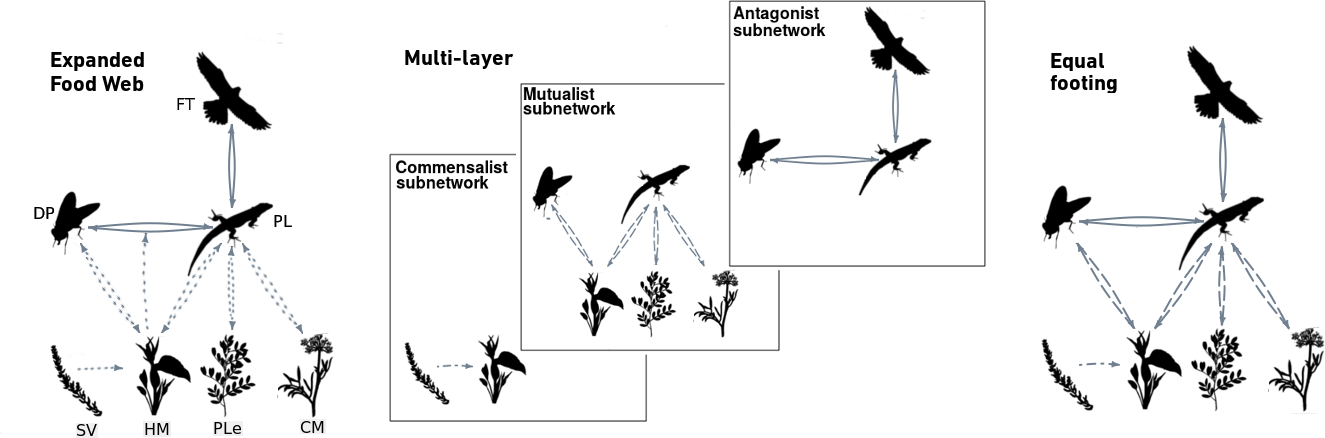
\includegraphics[width=\textwidth]{./Figures/chapter02/Fig_1.png}
\caption[Three approaches for multiple interactions networks]{\color{Gray} Three approaches for constructing and analyzing networks with multiple interaction types. In the first panel, solid lines represent trophic interactions, dotted lines non-trophic ones. Note that frugivory and pollination have both trophic and non-trophic components. In the second and third panels, solid lines represent antagonistic interactions, dashed lines mutualistic ones and dotted-dashed lines commensalistic ones. Data for building the network taken from the Aire Island community (see the Aire Island case study).}
\label{fig:fig2.1}
\end{figure}

\section{Multilayer Networks}
The concept of networks formed by different types of interactions (edges, more generally, connecting two individual nodes of the network) was first developed in the first decades of the 20th century in the field of social sciences, for characterizing social interaction networks with different types of relationships between individuals. Nevertheless, it is only in the last few years that the idea has been properly defined mathematically, given a consistent terminology, and applied to a wide variety of research objectives in, for example, engineering, economical or social networks (see the reviews by \citealt{Boccaletti2014} and \citealt{Kivela2014} to learn more about the history, methodology and applications of the paradigm).

The basic principle is that nodes within a network can be linked in different ways or in different contexts, so that the overall network contains two or more layers that represent different link types or other aspects of variation. Nodes can be connected to nodes of the same layer (intra-layer links) or to nodes of different layers (inter-layer links). Such multidimensional object is called - in it most general definition - a multilayer network. An ecological community in which different species interact in a discrete number of ways is a very intuitive example of such a network \citep{Pilosof2017}. In it, each interaction type would constitute a different layer within the {}'interaction type{}' aspect, and other potential layering aspects could be time (i.e. the realization of the network in different sampling campaigns) or site (different sampling plots).

Mathematically, a multilayer network consists on a quadruplet  $M=\left(V_M,E_M,V,L\right)$  . Its elements are, first, a sequence of sets of elementary layers  $\left\{L_a\right\}_{a=1}^d$  , where  $d$  is the number of layering aspects. The full set of nodes of the network,  $V$  , does not include the information about which node belongs to which layer, so a further set of node-layer tuples encodes this information:  $V_m{\subseteq}V\times L_1\times {\cdots}\times L_d$  . These node-layer tuples, i.e. the instances of a node in a given layer, are called {}'state nodes{}'. Lastly,  $E_m{\subseteq}V_M\times V_M$  is the set of intra-layer and inter-layer links. This minimal definition is expanded in the reviews by \cite{Kivela2014} and \cite{Pilosof2017}. When designing multiple interactions networks,  $d{\geq}1$  , as at least the layering relative to interaction type will be present; also, links may be constrained to {}'diagonal coupling{}', i.e. the situation in which a node will only be connected to itself in different layers. Representations where layers are not interaction types but some other grouping of the community are also possible (Appendix 2.2). For modelling the dynamics of multilayer networks, any dynamical model representing species interactions may be used in which sub-networks are represented by sets of equations and, depending on the design, auxiliary equations may be used to connect the different state nodes of a given entity, or state nodes of different entities in different layers. The inter-layer links of a multilayer network make this framework particularly versatile, as these may represent any kind of relationship between layers (see Appendix A.2.2: Figure A.2.2.3 for a definition of the different types of links in multilayer networks, and their matrix representation). For example, a link coupling the same plant species in pollination and herbivory sub-networks may represent the effect that consumption of reproductive organs by herbivores has in the interactions between the plant and its pollinators. Inter-layer links may also represent a coupling between layers with different temporal or spatial scales, thereby explicitly accounting for the temporal or spatial dimension of the networks. Note that this framework may accommodate networks with markedly different structures. For example, networks where virtually all links are intra-layer and the opposite, networks in which virtually all links are inter-layer, are both multilayer networks; also, networks whose nodes are present in every layer or in just one of them can fall under this framework.

Multilayer networks have been explored in a few studies of multiple interactions networks (Table \ref{tab:table1.1}), but their applicability in ecology goes far beyond these studies. For example, they have been successfully applied to reconstruct super (phylogenetic) trees \citep{vonHaeseler2012}, to study temporal and spatial variability in network structure, or to the analysis of ecological processes at different scales \citep{Pilosof2017} . Despite the potential of the multilayer framework for modelling ecological dynamics within and across layers, most studies listed in Table \ref{tab:table1.1} have only analysed static structural patterns, with the only exceptions being the studies by \cite{Stella2016}, who studied the dynamics of parasite spreading in multilayer ecological networks of varying structures, and by \cite{Gracia-Lazaro2018}, on the influence of inter-layer mutualistic interactions over layers of competitive interactions. In general, ecological studies on multilayer networks are starting to show that interactions other than predator-prey ones are also highly structured \citep{Melian2009,Kefi2015} and this topological structure has important consequences for different community properties \citep{Pocock2012, Evans2013a, Kefi2016a}.

As this approach has been developed mostly in theoretical physics and most reserachers in ecology may not be familiar with its terminology, a brief note is needed here. Following the definitions from \cite{Kivela2014}, a multilayer network is the most general object representing networks with multiple layering aspects and connections among layers. Although we focus on networks where the only layering aspect is interaction type and are diagonally-coupled, (termed `multiplex' networks or `edge-coloured multigraphs' in \citealt{Kivela2014}), we acknowledge that multiple interactions networks can also include other layering aspects and more complex patterns of inter-layer links. Therefore we adopt the more general term of multilayer networks in our review (Box 2). We will also use indistinctly the `layer' and `sub-network' terms to refer to a layer of specific interaction types in this framework.

\section{Equal Footing Networks}

Regardless of the specific characteristics or vital rates of an organism potentially modified by a pairwise interaction, its effects can be summed up as influencing either (1) individual fitness, (2) population size, or (3) population growth rate \citep{Abrams1987}. This view of interactions as aggregating effects over general individual or population-level parameters is the conceptual basis behind {}'equal footing networks{}', with the main consequence that pairwise interactions of any type can be measured and compared {}'on equal footing'.

A minimal population dynamics model can be represented as in Eq. 1. The main difference with the expanded food webs is that here, trophic and non-trophic interactions influence the intrinsic growth rate through the interaction terms of the adjacency matrix  $\left[a_{\mathit{xy}}\right]$  , instead of being modelled through auxiliary equations 2-3. Therefore, the adjacency matrix may include all pairwise combinations \{(0,0),(0,+),(0,-),(+,-),(+,+),(-,-)\} (Appendix A.2.2: Figure A.2.2.4).

Being a more general approach than expanded food webs, numerical models of equal footing networks are more scalable. Following Eq. 1, each species can be modelled by a single equation, and  $S^2+S$ parameters are required for a complete model of  $S$ species. This generality through the integration of fundamentally different interaction mechanisms in the adjacency matrix hinders the level of biological realism that can be achieved, in contrast with expanded food webs. By manipulating the signs of the adjacency matrix, different proportions of interaction types can be generated, but the effect of varying these proportions on community stability is an open question. \cite{Mougi2012} showed that, under certain conditions, local stability is enhanced for theoretical communities mixing antagonism and mutualism, as opposed to communities with a single interaction type. Their a priori conditions were that 1) mutualisms and antagonisms have, in total, the same effect over population growth rates and 2) for any species, the net effect of a given interaction decreases with increasing numbers of links of the same type. Two subsequent studies debated their conclusions: \cite{Suweis2014} stated that these conditions, and not the mixing of interaction types, were the factors that stabilized their models, whereas \cite{Kondoh2015} partially relaxed their initial assumptions and still found increasing stability with interaction mixing. Recently, the methodology developed in \cite{Mougi2012} has been expanded to assess the role of commensalism and amensalism \citep{Mougi2016a} and the potential switching of interactions \citep{Mougi2016b}, finding that separately accounting for these factors (unidirectional interactions and interaction switching) also increases local stability. The evaluation of equal footing networks through local stability analyses (for review see Table \ref{tab:table1.1}) is methodologically equivalent to the analysis of single-interaction networks. Hence, it is a natural approach for comparing networks of single and multiple interaction types without resorting to specific interaction mechanisms. In the studies already published (Table \ref{tab:table1.1}), different studies have considered different sets of interaction types and modelling assumptions, so that no integrative conclusions can be obtained at this point. Nevertheless, an emerging trend seems to be that networks with more than one interaction type and where different interactions are structured non-randomly are more locally stable than their single-interaction, non-structured counterparts.

The equal footing framework can be thought of as a particular type of multilayer network, in which the interaction layers are {}'flattened{}' in a single network, so that inter-layer links disappear, and each node is simultaneously affected by all interactions. \ This flattening is possible when three conditions are met: state nodes of the same node in the different layers of a multilayer network represent the same physical entity (as opposed to transportation networks, for example, where state nodes might represent bus or train stations of the same city), layers are diagonally-coupled, and all interactions in the different layers are expressed in the same units. This last condition is probably the most general, and in fact it represents our second criterion for distinguishing among frameworks. It allows the possibility of flattening multilayer networks in which there is link overlap among layers, as the overall effect will be a function of all layer-specific effects. We believe that these restrictive conditions, and the prevalence of equal footing networks in the theoretical studies listed in Table \ref{tab:table1.1}, merit the consideration of this framework as separated from the more general multilayer networks. The study by \cite{Melian2009} provides an example of a multilayer dataset flattened to an equal footing dynamic model.

\clearpage

\begin{small}
\begin{mdframed}
\subsection*{Box 1: Choosing a multiple interaction network methodology}
%\end{mdframed}
What constitutes a {}'realistic{}' representation of an ecological community? The answer is likely contingent on many factors, including the type of community being studied, the availability of empirical data and/or the ease to obtain it through observational or experimental studies. Although these factors, as well as research objectives and ecological assumptions, vary widely among studies, we propose a series of general guidelines for helping decide which multiple interactions framework is more appropriate for analyzing different types of data and questions (Fig. \ref{fig:fig2.1}).

The first dichotomy is whether the study involves structural and/or dynamical analyses (in this context, dynamical analyses refer to model-based projections of, at least, species abundances or biomass). In the first case, countless studies have analysed network structure based on lists of species and presence/absence of interactions between them. An excellent example of a structural analysis of a multiple interaction network is the comprehensive study of the Chilean rocky shore intertidal community by \cite{Kefi2015}. We suggest, for such analyses, arranging data according to the multilayer framework, which provides a versatile representation of the network and for which there is a well established, wide set of diagnostic metrics \citep{Pilosof2017}.

When values of biomass/abundance and interaction strengths are sampled or estimated (for example, based on allometric relationships, as in e.g. \cite{Kefi2016a}, community dynamics can be modelled. In these cases, the influence of the parameterization on the results obtained should be appropriately gauged against null models, but this topic is out of the scope of our study.

If interactions are classified in terms of their effect over a certain population parameter, either equal footing or multilayer networks are the appropriate modelling frameworks for analyzing dynamical systems. In this situation, choosing one approach over the other depends crucially on our second general criterion, i.e. the units in which interaction strengths are represented. Other factors may also play a role, for example the presence of multilink overlap (see case study), the complexity of inter-layer links, or whether the dynamics of single-interaction sub-networks may be of interest when considered as separate entities. Generalizing, if it is of any interest to consider interaction types separately (for example, if different interaction types are modelled through different functional forms and with different units) or there are complex inter-layer connections, multilayer networks should be used. If, on the other hand, the interest lies in the overall dynamics of the whole system, equal footing networks might be preferable.

The other branch of the flow chart in Fig. \ref{fig:box1.fig1} represents the situation where estimates of interaction strength are classified according to the mechanism they act upon. In this case, if the community consists of relatively few species or functional groups, each interaction can be modelled in detail, and the number of parameters might still be manageable: expanded food webs provide the most appropriate framework for such situations. Modelling the dynamics of a higher number of species, on the other hand, usually implies less mechanistic knowledge of the interactions within the community, and therefore interactions can be grouped in layers of a multilayer network that represent specific families of mechanisms. Notwithstanding these guidelines, as before, other factors may play a role (e.g. the inclusion of interaction modifiers, as in the case study). In all cases, selecting an appropriate framework will ultimately depend on the data at hand, the objectives of the study and the judgement and familiarity of the researchers with the different methodologies.

% within mdframed environments,another float environment does not work well
% so use custom captions of the memoir class
%\begin{figure}[h]
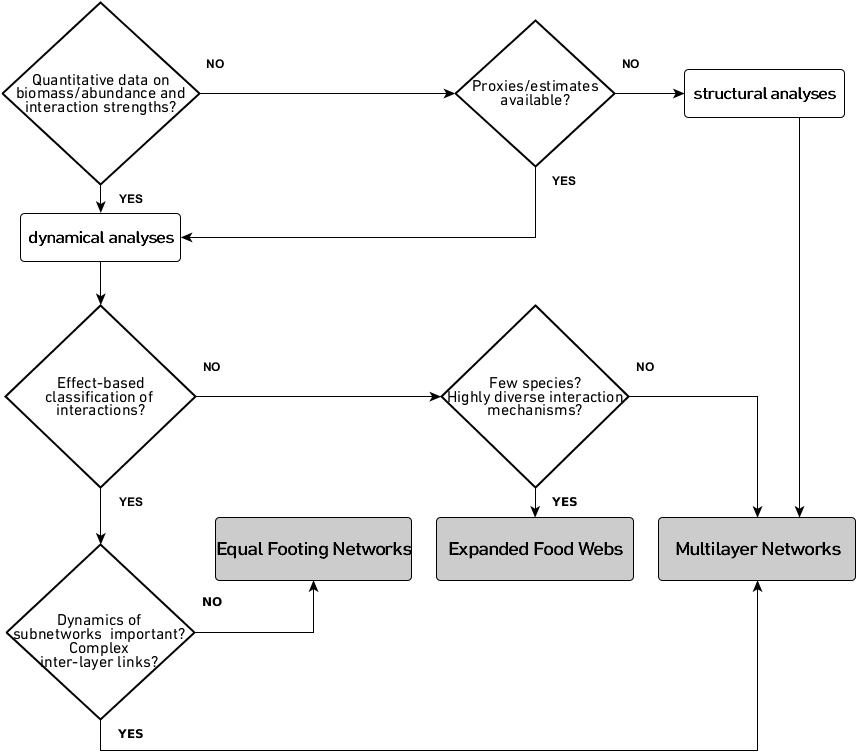
\includegraphics[width=.95\textwidth]{./Figures/chapter02/Box_1_Fig_1.png}
\figcaption[Choosing a multiple interaction network methodology]{\color{Gray} Diagram for choosing a multiple interaction network methodology, to be read starting from the upper left diamond box.}
%\caption}
\label{fig:box1.fig1}
%\end{figure}

\end{mdframed}
\end{small}

\section*{Acquisition and aggregation of empirical data}

Collecting data on the presence and strength of pairwise interactions in nature is notoriously difficult, even for the most easily observed interactions (Jordano 2016). It follows that interaction networks tend to be markedly under{}-sampled \citep{Chacoff2012}, and the proportion of type II errors, i.e. existing interactions that are not observed, is rarely known \citep{Olesen2011a, Morales-Castilla2015, Gravel2016}. In turn, quantifying the strength of observed interactions is also a long-standing challenge even for single interaction networks \citep{Berlow2004}. Several interaction strength indices have been developed by theoretical ecologists, but these are usually disconnected from the set of metrics obtained in field or manipulative studies \citep{Wootton2005}. Furthermore, very few pairwise interaction types have been extensively studied and their functional forms analysed (e.g. \citealt{Holland2002, Novak2008}), while the existence and/or dynamics of the vast majority of interactions in nature remain unknown. Thus, designing and implementing programs for collecting reliable data on multiple interaction types is presently one of the biggest challenges for community ecologists, up to the point that we are aware of just a handful of prominent examples in the literature. For example, \cite{Melian2009} aggregated data from several studies on pollination, seed dispersal and herbivory carried out between 1981-1984 in the Do\~nana Biological Reserve, in southern Spain. With that data, they constructed a network of 390 species and 798 interactions. Parasitic species and links, in addition to predator-prey interactions, were sampled by \cite{Hechinger2011} in food webs of three estuaries in the North American Pacific coast, in a dataset that included 314 species and 11270 interactions. In the study by \cite{Pocock2012}, several interaction types were concurrently sampled in different habitats of an agro{}-ecosystem in the UK, obtaining a network of 560 species and 1501 interactions. Finally, two networks of intertidal communities have been collected recently: \cite{Sander2015} obtained 1898 interactions between 110 taxa from the intertidal middle zone of Tatoosh Island based on observations and natural history of the species, and \cite{Kefi2015} took advantage of decades of work conducted on the marine rocky intertidal communities of the central Chilean coast to reconstruct its qualitative community network based on field observations and expert knowledge. Their network includes 104 species and 4754 interactions.

From these examples, one can distinguish two main strategies for constructing empirical multiple interactions networks: aggregating data from different sources of a given community in order to reconstruct the community network a posteriori (as in \citealt{Melian2009, Hechinger2011, Kefi2015} and \citealt{Sander2015}), or designing an integrated sampling program for a given set of previously defined interaction types, thus obtaining a realization of the network where all interactions are mostly co-occurring in space and time (as in \citealt{Pocock2012}). In the first approach, one may assemble information from studies conducted with different objectives and sampling methodologies and over different time periods, so that the aggregated network can potentially include a large fraction of the realized interactions, but these may or may not co-occur in time and/or space. Differential sampling efforts across studies will be unavoidable, and a posteriori analyses should be considered to minimize over or under-representation of certain clades and interactions. In the second approach, as fieldwork is likely to be conducted in tight time periods and in parallel for the different interaction types, sampling will potentially be more limited. On the other hand, this concurrent sampling is a more realistic snapshot of the co-occurring interactions in the sampling period, and importantly, fieldwork can be designed a priori to assign a near-homogeneous effort to different interaction types (but a posteriori corrections such as sample-based rarefaction are also advised; see \citealt{Pocock2012} and references therein). A non-exhaustive list of factors to account for the design of field campaigns is provided in Table \ref{tab:table1.2}, but a more comprehensive analysis of sampling strategies for multiple interactions networks is needed.

\begin{table} \footnotesize
\caption[Sampling of multiple interaction types]{\color{Gray}List of factors to consider in the design of sampling campaigns for multiple interaction types. These factors are general and independent from the framework chosen to represent the obtained network.}\label{tab:table1.2}
\begin{tabularx}{\textwidth}{p{2cm} X}
\hline
Factor & Examples of relevant questions\\
\hline
Temporal scale &
Single sampling campaign or periodic samples? What is the time scale of the interactions to be sampled? Are all/certain interaction types expected to vary along the sampling period?\\

Spatial scale &
What is the spatial scale of the interactions to be sampled? Are all/certain interaction types expected to vary spatially?\\

Habitat type(s) &
How many habitat types will be sampled? How does sampling effort vary across habitats? Which interaction types are expected to be prevalent in each habitat type?\\

Interaction types &
Which interaction types are expected to be sampled? Which sampling methodologies are applied to capture them? How does the proportion of forbidden links vary among interaction types?\\

Field and experimental observations &
Are experimental observations needed for observing specific interaction types (e.g. for estimating the prevalence of parasitism, or the number of flowers visited by a given pollinator)? How is effort distributed among field and experimental observations?\\

Natural history of species &
Do species in the community have varying activity periods or phenologies? Are there significant differences in mobility, behaviour, and other traits relevant to the probability of observing an interaction?\\

Movement capacity &
Will network include permanent species or also transient ones? How is a permanent species defined?\\
\hline

\end{tabularx}

\end{table}

Regarding the key issue of estimating empirical interaction strengths, it is often necessary to conduct manipulative experiments for obtaining reliable functional forms and interaction strength coefficients. Such experiments, however, are very context and clade-specific, and usually pose increased costs and logistical difficulties over field observations. For these reasons, a growing line of research is being developed for, given minimal information, inferring the presence \citep{Morales-Castilla2015, Deyle2016} and strength \citep{Novak2008, Berlow2009, Vazquez2012} of biotic interactions. Specifically, an interaction strength proxy that may be applicable to different types of interactions is the frequency of occurrence of an interaction. \cite{Poisot2015} proposed a general framework for integrating dynamic interaction strengths in dynamical models, taking into account the long-held idea that the net impact of a species over another can be described as a function of two components: the frequency of interaction and the per interaction effect \citep{Vazquez2005}. Thereby, the relative role of density-mediated and trait-mediated effects on direct interactions can be explicitly analysed. So far, it has been hypothesized that the net impact of mutualistic plant-pollinator interactions can be approximated by their frequency for both sides of the interaction \citep{Vazquez2005,Vazquez2012} and, in addition, that the asymmetry among interaction strengths is well explained in some cases solely by species' relative abundances (for quantitative bipartite networks, as in \citealt{Vazquez2007}). These ideas converge towards a unified neutral view of ecological interactions: interactions can be approximated as being the result of random encounters among individuals, whose probability is mediated by the relative abundances of the populations involved \citep{Araujo2014, Canard2012, Canard2014, Cazelles2016}. The frequency of interactions will naturally equal the net impact of a population over another, since per capita interaction strength will not vary with other factors (traits, environmental conditions). Further research is needed to test the robustness of (1) species abundance as a proxy for interaction frequency, and (2) interaction frequency as a proxy for interaction strength.

\begin{mdframed}
\begin{small}

\subsection*{Box 2: Definitions of key terms}

The approach used for classifying interactions does not only have methodological consequences: it is above all constrained by the very definition of interaction. Hence, it is important to be clear and explicit about the definitions used.

The ones we use in this study for direct and indirect interactions are taken directly from \cite{Abrams1987}. These definitions can be applied both to effect-based and mechanism-based classifications, and though we define indirect interactions for completeness, we mainly focus on direct interactions.

For effect-based classifications, existing definitions are complete, as they cover the full spectrum of possible combinations of interactions in what can be described as the biotic interaction space \citep{Araujo2014}. New terms have been introduced with time, e.g. expanding the definition of (+,-) interactions originally described as being mainly characterized by predation to, first, contramensalism \citep{Arthur1989} and later, antagonism \citep{Sousa1993}.

Within mechanism-based classifications the situation is somewhat more convoluted. In such studies, it is commonplace to study trophic and non-trophic interactions separately. Although defining these terms is apparently trivial, we have encountered very different implicit meanings of what constitutes a non-trophic interaction in the literature. For example, in the studies by \cite{Arditi2005} and \cite{Goudard2008}, non-trophic interactions are defined as modifiers of trophic interactions. \cite{Prasad2010} consider non-trophic interactions to be `driven by one species changing the behaviour but not the density of another species'. Finally, \cite{Kefi2012} interprets non-trophic interactions as being all other interactions than feeding ones, including the non-trophic components of pairwise interactions such as pollination or frugivory. We adopt the latter definition, as it more clearly fits within a simple generalizable framework, although it requires certain interactions to be split in their trophic and non-trophic components. Lastly, effect-based and mechanism-based classifications need not be mutually exclusive \citep{Abrams1987}: it is common for effect-based interaction classes to be divided according to specific ecological mechanisms, e.g. mutualisms can be divided by considering whether there is a trophic component in them or not, etc.

\begin{description}
\item[Interaction] A change in some characteristic of a population mediated by properties or actions by individuals of other population.

\item[Direct interaction] Interaction in which the effect occurs either through direct physical contact or through a third set of entities produced by one of the two interactors.

\item[Indirect interaction] Interaction in which the effect occurs as a result of other effects produced by one interactor on some population property of a third set of entities; and the third set of entities is not produced by any of the interactors.

\item[Trophic interaction] In the context of mechanism-based classifications, an interaction (or component of one) that involves direct exchange of energy (biomass) between the two individuals.

\item[Non-trophic interaction] In the context of mechanism-based classifications, an interaction (or component of one) that does not involve exchange of energy (biomass) between the two interacting individuals.

\item[Single-interaction network] Ecological network in which one interaction type is considered. Classic examples are food webs or plant-pollinator networks.

\item[Multiple interaction network] Ecological network with more than one interaction type. This umbrella term includes any topology and/or classification of interactions.

\item[Expanded food web] Multiple interaction network in which consumer-resource interactions form the basic structure of the network. Other interactions are termed ``non-trophic'' interactions and may affect any parameter of the dynamic model.

\item[Multilayer network] Network with different types of connections between nodes. In an ecological context, different network layers commonly represent different interaction types. If there is only one layering aspect and nodes are diagonally-coupled, that type of multilayer network is termed multiplex.

\item[Equal footing network] Multiple interaction network in which all interaction types are expressed in the same units, i.e. influence the same parameter of the dynamic model.

\end{description}
\end{small}
\end{mdframed}

\section*{The Aire Island case study}

The expanded food web, multilayer and equal footing frameworks for building multiple interactions networks offer complementary insights for the study of ecological communities, and each one is best suited to different types of studies and objectives (Box 1). Here, to demonstrate the diversity of ecological questions that can be addressed with multiple interactions networks, we analyse an empirical community under the lenses of each one of the approaches described. Specifically, we ask:

\begin{enumerate}
\item what is the influence of non-trophic interactions on the local abundances of all species? (expanded food web approach);
\item which species serve as ``hubs'' for linking species through interaction sub-networks and in the overall network? (multilayer network approach);
\item does the strength of different interaction types influences local community stability?(equal footing approach).
\end{enumerate}

The community examined is located on the Aire Island, a small islet located SE off the coast of Menorca (Balearic Islands, Spain) with an area of around 342500 m{\texttwosuperior}. Almost the entire surface of this relatively flat islet is exposed to the effect of the sea. Therefore, most vegetation is halophilous (i.e. thrives in saline environments) except in areas sheltered from wind and sea, where typical Mediterranean species appear, such as Pistacia lentiscus \citep{Perez-Mellado2006}. Our examples are based on a subset of the ecological community of this islet.

A remarkable set of interactions has been unveiled in the Aire Island between the dead horse arum (\textit{Helicodiceros muscivorus}), its associated insect pollinators (Diptera, genus \textit{Calliphora} and \textit{Lucilia}), and the Balearic lizard, \textit{Podarcis lilfordi}. The Balearic lizard is an omnivorous lacertid of medium size, endemic to the Balearic Islands. It has been shown to bask on the spathe of \textit{Helicodiceros muscivorus} {}' flowers, and to feed on the pollinating flies attracted by the intense odour produced by the plant. In addition to this negative effect of \textit{Podarcis lilfordi} on \textit{Helicodiceros muscivorus} through consumption of potential pollinators, it is itself an effective seed disperser of the plant: \textit{Podarcis lilfordi} consumes ripe fruits of \textit{Helicodiceros muscivorus} routinely, and seeds dispersed by the lizard show a significantly higher probability of germination than non-consumed seeds \citep{Perez-Mellado2006}. \textit{Podarcis lilfordi} is also an effective pollinator of other species at Aire Island. Particularly, high loads of pollen from \textit{Pistacia lentiscus} and \textit{Crithmum maritimum} have been found in lizard's bodies in previous studies on the same community \citep{Perez-Mellado2000}. Due to the scarcity of natural predators, \textit{Podarcis lilfordi} reaches high densities in the islet \citep{Perez-Mellado2008}. Its main predator is probably the Eurasian Kestrel (\textit{Falco tinnunculus}), that does not nest on the islet but visits it frequently. Lastly, the appearance of \textit{Helicodiceros muscivorus} is related to the percentage of soil covered by \textit{Suaeda Vera}, an hallophylous shrub of the Chenopodiaceae family, suggesting facilitation by the shrub on the development of \textit{Helicodiceros muscivorus} \citep{Perez-Mellado2006}. The interaction network formed by these 7 species (or guild, in the case of the Diptera) spans 3 trophic levels, and includes antagonistic, mutualistic and commensalistic interactions. In the following equations and figures, $S$ refers to the whole set of species, and species are denoted by their initials or silhouettes. When available, we use empirical data for parameter estimates. Whenever empirically derived estimates are unavailable, as these examples are only to illustrate the approaches, we assign values based on our judgements of plausibility.

\subsection*{Expanded food webs: Influence of non-trophic interactions in equilibrium abundances}

The main strength of the expanded food webs is the inclusion of detailed, mechanistic, non-trophic interactions in the general food web structure. We investigated their influence in the resulting abundance patterns of the community, compared to a standard food web model.

The continuous-time model for the expanded food web considers only three ecological processes: growth, mortality, and pairwise interactions, which can be trophic or non-trophic. Trophic interactions can, themselves, be modified by the presence of a third species. The main equations are of the form:

\begin{equation} \label{eq:2.4}
\frac{\mathit{dN}_x}{\mathit{dt}}=r_xN_x-m_xN_x^2+\sum _{y{\in}S,y{\neq}x}a_{\mathit{xy}}N_xN_y
\end{equation}

where  $r_x$  is the short-term per capita growth rate,  $m_x$ is the per capita mortality rate (that, multiplied by  $N_x^2$  , acts as a self-limitation term) and  $a_{\mathit{xy}}$  are the pairwise trophic interaction coefficients (the partial derivative of the per capita growth rate of species  $x$  with respect to the density of species  $y$  ).

Several non-trophic interactions are included on top of this general structure, affecting either  $r_x$ ,  $m_x$ or  $a_{\mathit{xy}}$ . As an example, the modification of the mortality rate is modelled with a saturating function \citep{Kefi2012}

\begin{equation} \label{eq:2.5}
m_x\left(N_y\right)=\frac{m_x^{\mathit{NTI}}N_y+m_x^0N_y^0}{N_y+N_y^0}
\end{equation}

The function varies between a basal value $m_x^0$ when $N_y=0$ , i.e. in the absence of non-trophic interactions, and  $m_x^{\mathit{NTI}}$ when the non-trophic interaction is highest. The same equation was used to model non-trophic interactions influencing the other parameters of Eq. 6 (growth rates  $r_x$ and interaction coefficients  $a_{\mathit{xy}}$ ). For modelling the Aire Island community, we assumed that (1) all mutualistic interactions positively affect short-term growth rates, i.e. $r_x^{\mathit{NTI}}>r_x^0$ for \textit{Helicodiceros muscivorus}, \textit{Podarcis lilfordi}, Diptera, \textit{Pistacia lentiscus} and \textit{Crithmum maritimum}; (2) the presence of \textit{Suaeda vera} increases the survival probability of \textit{Helicodiceros muscivorus} seedlings by providing a favorable microhabitat, thus decreasing the mortality rate of the facilitated plant, i.e. $m_{\mathit{HM}}^{\mathit{NTI}}<m_{\mathit{HM}}^0$ ; and (3) increases in abundance of \textit{Helicodiceros muscivorus} increased the magnitude of the predator-prey interaction between \textit{Podarcis lilfordi} and the Diptera species, i.e. $a_{\mathit{PL},\mathit{DP}}^{\mathit{NTI}}>a_{\mathit{PL},\mathit{DP}}^0$ and $a_{\mathit{DP},\mathit{PL}}^{\mathit{NTI}}<a_{\mathit{DP},\mathit{PL}}^0$.

The complete parameterizations of the expanded food web model and the equal footing model are included in Appendix 2.1. We found significant differences in abundances at equilibrium for all species except \textit{Suaeda vera}, depending on the set of interactions considered (Fig. \ref{fig:fig2.2}). We define equilibrium as the steady state reached after a sufficient number of time steps (2500 in our case). Non-trophic interactions in the Aire Island community are all positive, and accordingly, all populations increase in equilibrium abundance when engaging in non-trophic interactions. The only organism that conceivably could be negatively affected by the inclusion of non-trophic interactions are the Diptera, given that the magnitude of the \textit{Podarcis lilfordi} - Diptera antagonism is enhanced by higher abundance of \textit{Helicodiceros muscivorus}. With the parameterization chosen, however, the positive influence of the Diptera -- \textit{Helicodiceros muscivorus} mutualism outweighs this increase (Fig. \ref{fig:fig2.2}, note the increase in Diptera abundance when non-trophic interactions are considered). Note that this is the only approach in which we explicitly model the influence of \textit{Helicodiceros muscivorus} populations in the predator-prey interaction between the Diptera species and \textit{Podarcis lilfordi}.

\begin{figure}[ht]
\centering
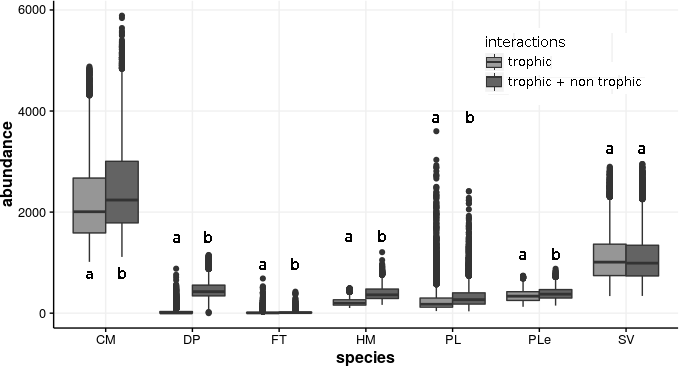
\includegraphics[width=\textwidth]{./Figures/chapter02/Fig_2.png}
\caption[Expanded Food Web analysis]{\color{Gray} Equilibrium abundances of the Aire Island community when considering trophic interactions, or trophic and non-trophic ones. Boxplots with different letters are significantly different according to Wilcoxon rank-sum tests (CM: W = 38176000, p {\textless} 0.05; DP: W = 63730000, p {\textless} 0.05; FT: W = 38512000, p {\textless} 0.05; HM: W = 57170000, p {\textless} 0.05; PL: W = 42005000, p {\textless} 0.05; PLe: W = 38454000, p {\textless} 0.05; SV: W = 31595000, p = 0.059).}
\label{fig:fig2.2}
\end{figure}

\subsection*{Multilayer networks: Importance of each species in structuring the network}

The role of the different species in structuring a given community has been extensively assessed for single-interaction networks \citep{Coux2016} and for multilayer networks in other fields \citep{Sole-ribalta2014,DeDomenico2015a}. For the multilayer framework, several metrics have been adapted directly from single-interaction networks and others have been defined taking into account the multidimensional nature of the multilayer approach \citep{DeDomenico2015a}. Among these novel metrics, the concept of multidegree is a multidimensional extension of the degree of a single-interaction network, that may help uncover important, well-connected species in each sub-network and in the overall structure. Here we calculate multidegrees as defined in \cite{Boccaletti2014}, where formal definitions are provided.

For understanding the concept of multidegrees, we first need to define the multilinks of the network. Multilinks (or multiedges) are links connecting two nodes in a combination of layers. For example, the Aire Island network has three interaction types. A multilink of the form (1,0,0) exists between two species if these species are connected in the first layer and not in the second or third one. One can see thus that the number of potential multilinks between any two species in a general network with  $M$  layers is  $2^M$  . The multidegrees  $m_x^i$ of species  $i$ are its number of multilinks of type  $x$, and its aggregation,  $m^i$  , is the overall multidegree as considered e.g. in \cite{Stella2016}.

Given three layers representing interaction types \{antagonism, commensalism, mutualism\}, the multilinks for the Aire Island network are:

\begin{equation*}
\begin{matrix}m_0=\{0,0,0\}\\m_1=\{0,0,1\}\\m_2=\{0,1,0\}\\m_3=\{0,1,1\}\\m_4=\{1,0,0\}\\m_5=\{1,0,1\}\\m_6=\{1,1,0\}\\m_7=\{1,1,1\}\end{matrix}
\end{equation*}

where  $m_0$ is the null multilink, representing the situation in which two species are not connected in any layer, and subsequently,  $m_7$ represents a multilink whereby two species are connected in the three layers. The number of shared multilinks between any two species can be represented by multi-adjacency matrices. The multi-adjacency matrices of the Aire Island community are:

\begin{equation*}
A^{m_0}=\begin{matrix}\text{ }\\\left.\phantom{\begin{matrix}\mathit{FT}\\\mathit{PL}\\\mathit{DP}\\\mathit{HM}\\\mathit{SV}\\\mathit{PLe}\\\mathit{CM}\end{matrix}}\right(\end{matrix}\begin{matrix}\mathit{FT}&\mathit{PL}&\mathit{DP}&\mathit{HM}&\mathit{SV}&\mathit{PLe}&\mathit{CM}\\0&0&1&1&1&1&1\\0&0&0&0&1&0&0\\1&0&0&0&1&1&1\\1&0&0&0&0&1&1\\1&1&1&0&0&1&1\\1&0&1&1&1&0&1\\1&0&1&1&1&1&0\end{matrix}\begin{matrix}\text{ }\\\left)\phantom{\begin{matrix}\mathit{FT}\\\mathit{PL}\\\mathit{DP}\\\mathit{HM}\\\mathit{SV}\\\mathit{PLe}\\\mathit{CM}\end{matrix}}\right.\end{matrix}\begin{matrix}\text{ }\\\mathit{FT}\\\mathit{PL}\\\mathit{DP}\\\mathit{HM}\\\mathit{SV}\\\mathit{PLe}\\\mathit{CM}\end{matrix}
\end{equation*}

\bigskip

\begin{equation*}
A^{m_1}=\begin{matrix}\text{ }\\\left.\phantom{\begin{matrix}\mathit{FT}\\\mathit{PL}\\\mathit{DP}\\\mathit{HM}\\\mathit{SV}\\\mathit{PLe}\\\mathit{CM}\end{matrix}}\right(\end{matrix}\begin{matrix}\mathit{FT}&\mathit{PL}&\mathit{DP}&\mathit{HM}&\mathit{SV}&\mathit{PLe}&\mathit{CM}\\0&0&0&0&0&0&0\\0&0&0&1&0&1&1\\0&0&0&1&0&0&0\\0&1&1&0&0&0&0\\0&0&0&0&0&0&0\\0&1&0&0&0&0&0\\0&1&0&0&0&0&0\end{matrix}\begin{matrix}\text{ }\\\left)\phantom{\begin{matrix}\mathit{FT}\\\mathit{PL}\\\mathit{DP}\\\mathit{HM}\\\mathit{SV}\\\mathit{PLe}\\\mathit{CM}\end{matrix}}\right.\end{matrix}\begin{matrix}\text{ }\\\mathit{FT}\\\mathit{PL}\\\mathit{DP}\\\mathit{HM}\\\mathit{SV}\\\mathit{PLe}\\\mathit{CM}\end{matrix}
\end{equation*}

\bigskip

\begin{equation*}
A^{m_2}=\begin{matrix}\text{ }\\\left.\phantom{\begin{matrix}\mathit{FT}\\\mathit{PL}\\\mathit{DP}\\\mathit{HM}\\\mathit{SV}\\\mathit{PLe}\\\mathit{CM}\end{matrix}}\right(\end{matrix}\begin{matrix}\mathit{FT}&\mathit{PL}&\mathit{DP}&\mathit{HM}&\mathit{SV}&\mathit{PLe}&\mathit{CM}\\0&0&0&0&0&0&0\\0&0&0&0&0&0&0\\0&0&0&0&0&0&0\\0&0&0&0&1&0&0\\0&0&0&1&0&0&0\\0&0&0&0&0&0&0\\0&0&0&0&0&0&0\end{matrix}\begin{matrix}\text{ }\\\left)\phantom{\begin{matrix}\mathit{FT}\\\mathit{PL}\\\mathit{DP}\\\mathit{HM}\\\mathit{SV}\\\mathit{PLe}\\\mathit{CM}\end{matrix}}\right.\end{matrix}\begin{matrix}\text{ }\\\mathit{FT}\\\mathit{PL}\\\mathit{DP}\\\mathit{HM}\\\mathit{SV}\\\mathit{PLe}\\\mathit{CM}\end{matrix}
\end{equation*}

\bigskip

\begin{equation*}
A^{m_4}=\begin{matrix}\text{ }\\\left.\phantom{\begin{matrix}\mathit{FT}\\\mathit{PL}\\\mathit{DP}\\\mathit{HM}\\\mathit{SV}\\\mathit{PLe}\\\mathit{CM}\end{matrix}}\right(\end{matrix}\begin{matrix}\mathit{FT}&\mathit{PL}&\mathit{DP}&\mathit{HM}&\mathit{SV}&\mathit{PLe}&\mathit{CM}\\0&1&0&0&0&0&0\\1&0&1&0&0&0&0\\0&1&0&0&0&0&0\\0&0&0&0&0&0&0\\0&0&0&0&0&0&0\\0&0&0&0&0&0&0\\0&0&0&0&0&0&0\end{matrix}\begin{matrix}\text{ }\\\left)\phantom{\begin{matrix}\mathit{FT}\\\mathit{PL}\\\mathit{DP}\\\mathit{HM}\\\mathit{SV}\\\mathit{PLe}\\\mathit{CM}\end{matrix}}\right.\end{matrix}\begin{matrix}\text{ }\\\mathit{FT}\\\mathit{PL}\\\mathit{DP}\\\mathit{HM}\\\mathit{SV}\\\mathit{PLe}\\\mathit{CM}\end{matrix}
\end{equation*}

\bigskip

\begin{equation*}
A^{m_3}=A^{m_5}=A^{m_6}=A^{m_7}=0
\end{equation*}

The multidegrees of the seven species of the community are the number of multilinks incident to them (Table \ref{tab:table1.3}). These metrics show that \textit{Podarcis lilfordi} is the most connected species, overall and both in the mutualist and antagonist sub-networks. \textit{Helicodiceros muscivorus} and Diptera are the following species in multidegree, and their links also span two layers. All other species are represented only in one layer, and are only connected to \textit{Podarcis lilfordi}, inviting the interpretation that the Balearic lizard has a disproportionate importance in structuring the community. In our small community, these results are visually evident, but the multidegree concept can be very useful in highly populated networks, where the importance of different species across layers is not obvious from visual inspection of the data. Note that by decomposing the overall multidegree into the contributions of each multilink we are able to evaluate the potential link overlap of any pair of species in any combination of layers. In our simple example, however, there is no overlap, a reasonable assumption when considering an effect-based classification of interactions over a single population parameter, since the potential partial positive and negative effects of a species over another are aggregated in order to calculate the net effect and the associated interaction type. For example, looking again at the \textit{Podarcis} -- \textit{Helicodiceros} interaction, the net direct effect of the lizard over the plant could be decomposed in, at least, 1) a negative effect due to the consumption of fruits (i.e. the trophic part of the pairwise interaction), 2) another negative effect due to the predation of potential Diptera pollinators, 3) the positive effect on seed dispersal, and 4) a further positive effect on survival of seeds that have been dispersed by \textit{Podarcis lilfordi} as opposed to seeds that germinate naturally. In the absence of more detailed experiments, and as suggested by \cite{Perez-Mellado2006}, we considered the overall effect of \textit{Podarcis lilfordi} over \textit{Helicodiceros muscivorus} to be positive. Link overlap in interactions can be expected when two species interact in different ways, for example due to varying ecologies of life stages, and more generally when the temporal dimension is included in the analyses.

\begin{table} \small
\caption[Multidegrees of the Aire Island multilayer network]{\color{Gray}Multidegrees of the seven species of the Aire Island multilayer network. Note that the trivial $m_0$ multilink represents no connections, so it is not considered for calculating the overall multidegree $m$.}\label{tab:table1.3}
\begin{tabularx}{\textwidth}{p{4cm}XXXXXXXXX}
\hline
& $m_0$ & $m_1$ & $m_2$ & $m_3$ & $m_4$ & $m_5$ & $m_6$ & $m_7$ & $m$\\ \hline
Falco tinnunculus & 5 & 0 & 0 & 0 & 1 & 0 & 0 & 0 & 1\\
Podarcis lilfordi & 1 & 3 & 0 & 0 & 2 & 0 & 0 & 0 & 5\\
Diptera & 4 & 1 & 0 & 0 & 1 & 0 & 0 & 0 & 2\\
Helicodiceros \ muscivorus & 3 & 2 & 1 & 0 & 0 & 0 & 0 & 0 & 3\\
Suaeda vera & 5 & 0 & 1 & 0 & 0 & 0 & 0 & 0 & 1\\
Pistacia lentiscus & 5 & 1 & 0 & 0 & 0 & 0 & 0 & 0 & 1\\
Crithmum maritimum & 5 & 1 & 0 & 0 & 0 & 0 & 0 & 0 & 1\\ \hline
\end{tabularx}

\end{table}


\subsection*{Equal footing networks: Influence of the magnitude of mutualistic and antagonistic interactions on community stability}

For assessing the effect of the strength of different interaction types on the overall stability of the network, we modelled the community using the equal footing framework. We used the continuous-time logistic equations proposed by \cite{Garcia-Algarra2014}, in which all extrinsic effects -- environmental, biotic interactions -- fall on the intrinsic growth rate  $r_x$ :

\begin{equation} \label{eq:6}
\frac{\mathit{dN}_x}{\mathit{dt}}=r_xN_x
\end{equation}

where

\begin{equation} \label{eq:7}
r_x=r_x^0+\sum _{y{\in}S,y{\neq}x}a_{\mathit{xy}}N_y-\left(\beta _x+c_x\sum _{y{\in}S,y{\neq}x}a_{\mathit{xy}}N_y\right)N_x
\end{equation}

The rightmost term of Eq.9 represents the self-limitation term. In the absence of pairwise interactions, the parameter $\beta _x$ controls self-limitation, and $c_x$ is a proportionality constant. Pairwise interaction coefficients  $a_{\mathit{xy}}$ were assumed constant. For assessing the relative influence of different interaction types on community stability, we varied the relative magnitude of facilitative (commensalistic and mutualistic interactions) and antagonistic coefficients and analysed the resulting local stability patterns of the system by examining the sign of the leading eigenvalue of the associated Jacobian matrix (Fig. \ref{fig:fig2.3} and Appendix A.2.3: Figure A.2.3.2).

Parameterizations with weak antagonistic interactions were virtually all stable (19991 out of 20000 replicates), regardless of the magnitude of facilitative interaction strength (Fig. \ref{fig:fig2.3}, groups a and b). Communities parameterized with strong antagonistic interactions (group c in Fig. \ref{fig:fig2.3}), on the other hand, were mostly unstable, with only 20 out of 10000 replicates having a leading eigenvalue {\textless} 0. All unstable communities were also unfeasible in that either key species went extinct or some species grew unbounded despite the self-limitation term of Eq. 9. Interaction strength magnitudes were chosen arbitrarily, in the absence of empirical data, but patterns were robust to variations of +- 2 orders of magnitude. Our results therefore suggest that increasing antagonist interaction strengths for this particular community would lead to instability. Bear in mind, though, that local stability analyses are only an approximation of ecological stability, as they only apply to closed systems in equilibrium. If accepting this assumption, local instability in the Aire Island community could be interpreted as being triggered by increased per capita antagonistic interaction strengths. These could appear, for example, if sexual dimorphism in \textit{Podarcis lilfordi} led to higher predation of females by birds, thus exerting a higher influence on population growth rate. This, however, does not seem to be case, since the only dimorphism reported in Aire Island is the slightly larger body size of males \citep{Perez-Mellado2000}; hence, no differential predation is expected.


\begin{figure}[!ht]
\centering
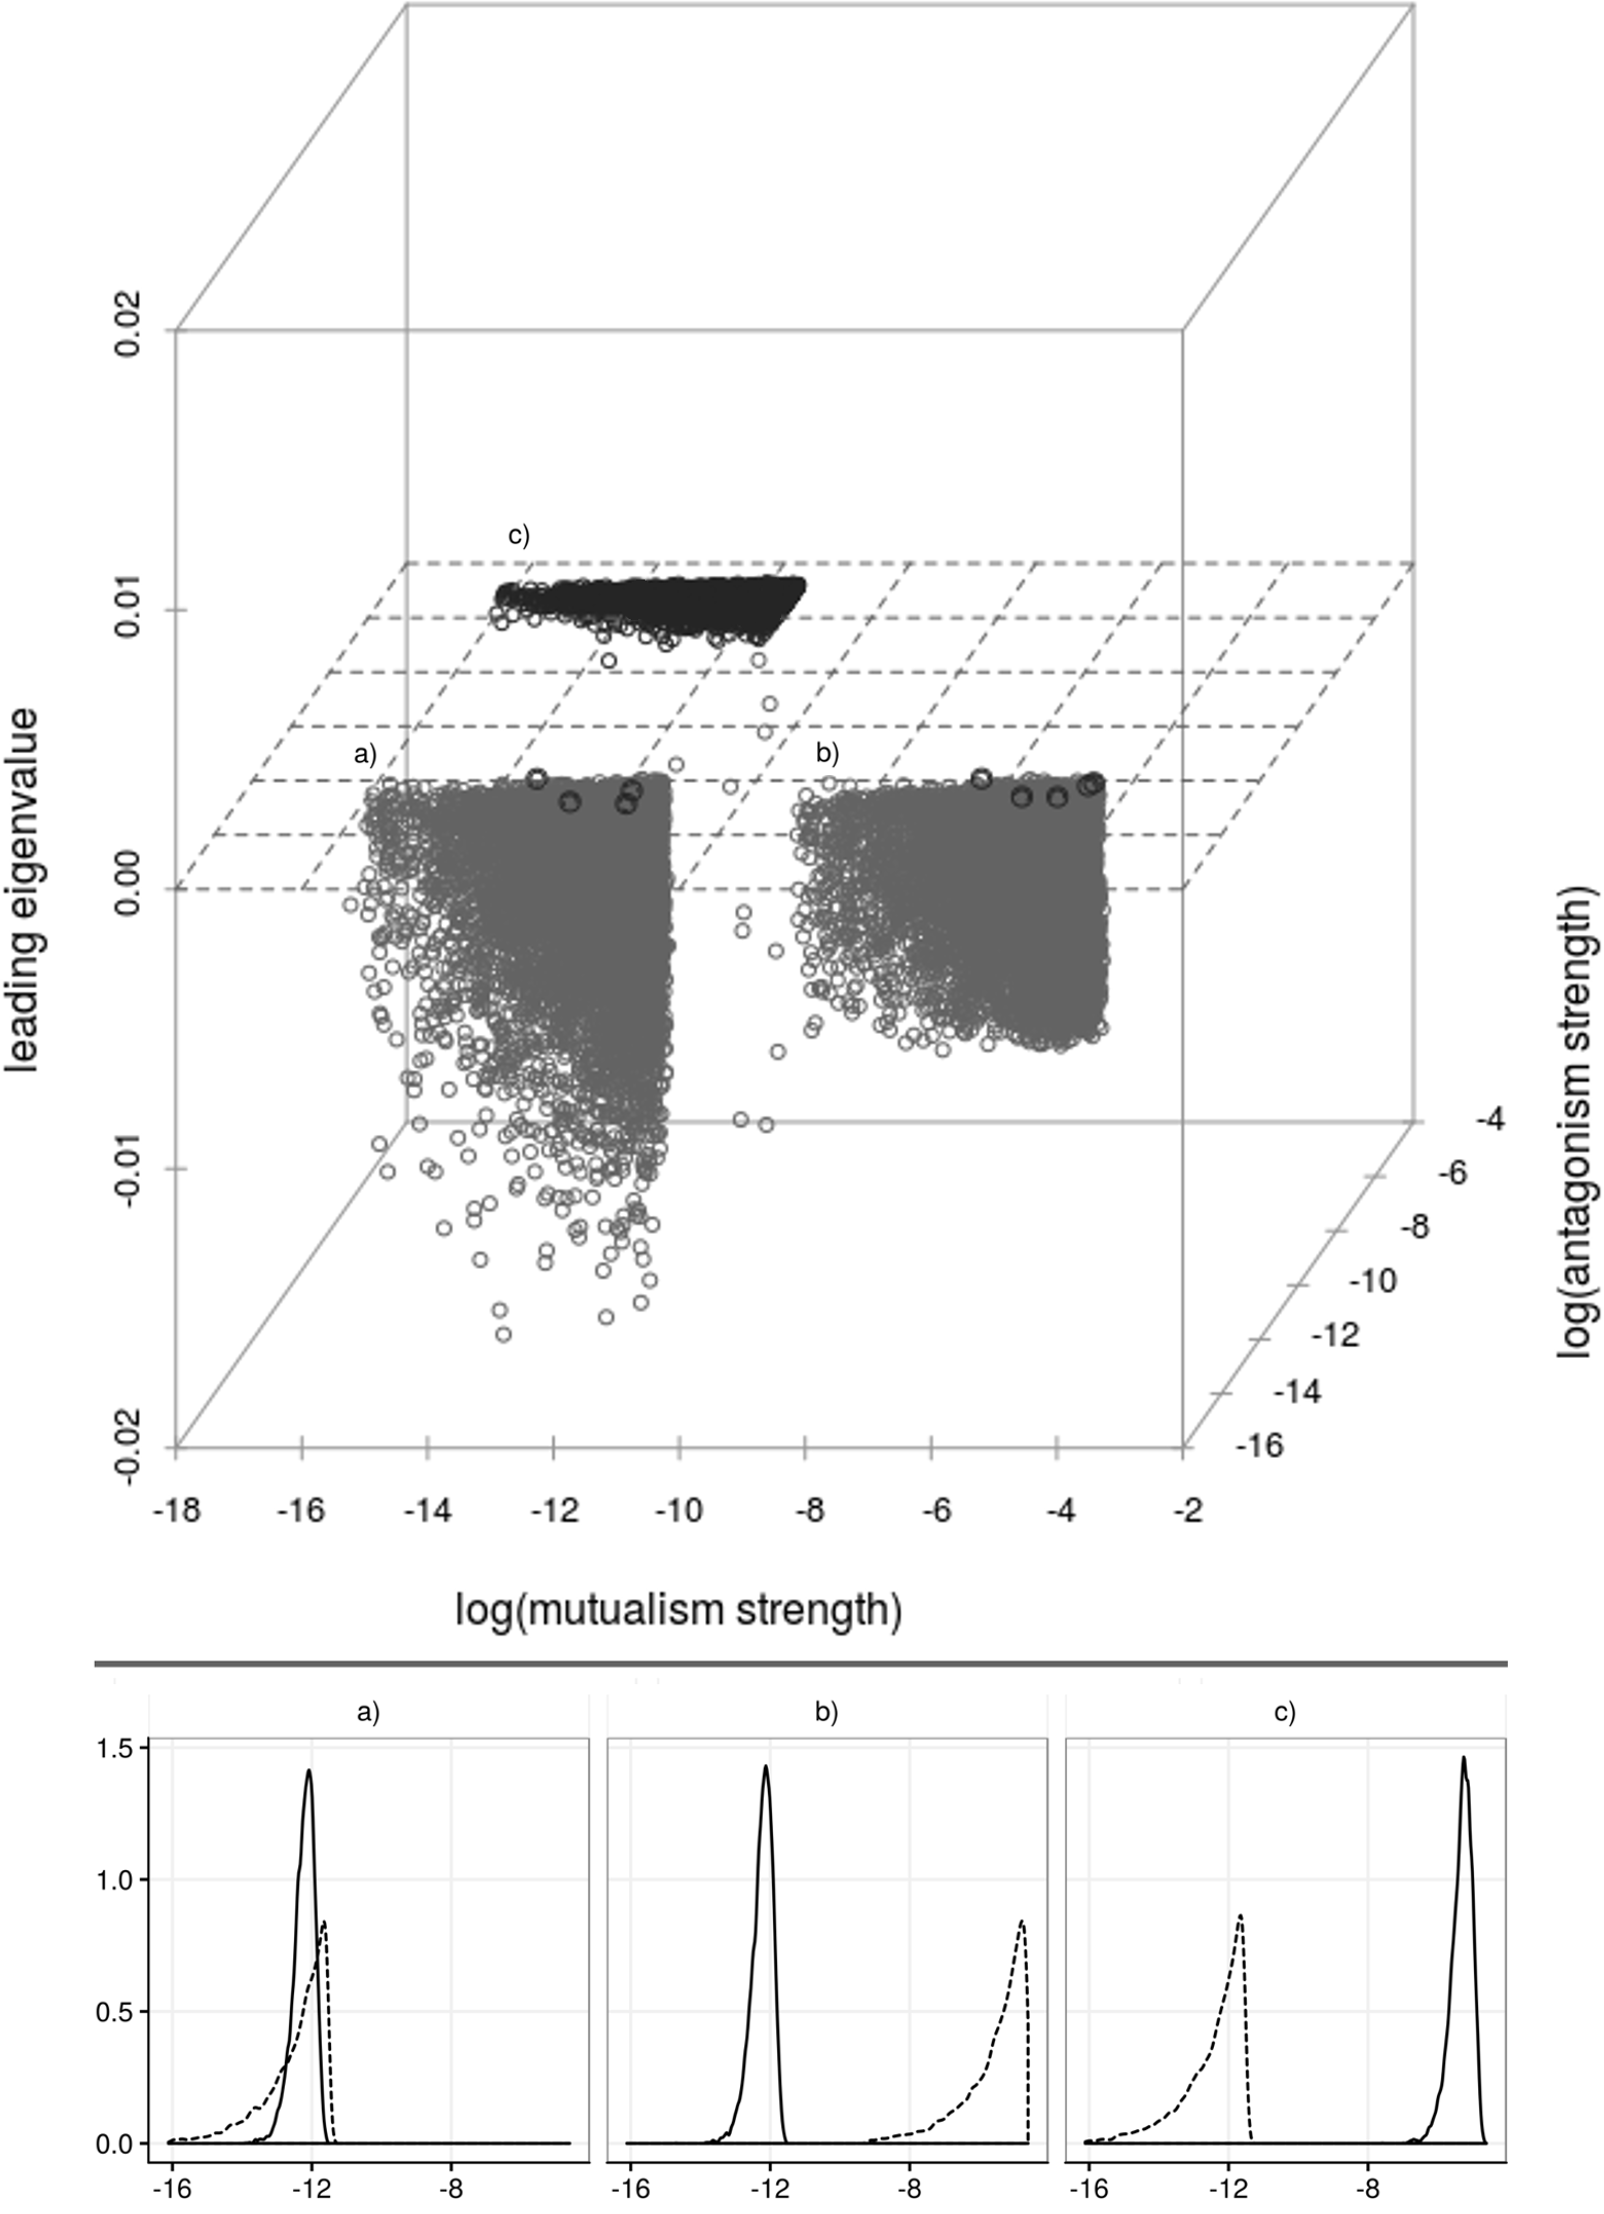
\includegraphics[width=.75\textwidth]{./Figures/chapter02/Fig_3.png}
\caption[Equal footing network analysis]{\color{Gray} Distribution of antagonistic and mutualistic interaction strengths and the leading eigenvalue of the resulting system. In the scatterplot, grey circles are systems with leading eigenvalue < 0, and black circles are systems with leading eigenvalue > 0. Group a) is the group of simulations with weak antagonistic and facilitative interactions; group b) are simulations with weak antagonistic and strong facilitative interactions; group c) are simulations with strong antagonistic and weak facilitative interactions. Within group c) only eigenvalue magnitudes close to 0 are shown, due to the extreme variability of the raw data (with values up to $10^99$ ). The rest of the data is shown in Appendix A.2.3: Figure A.2.3.2. For reference, a grid is drawn representing the z = 0 plane. Lower panels show the density distribution, for each group, of the logarithm of antagonist interaction strengths (solid lines) and the logarithm of facilitative interaction strengths (dashed lines).}
\label{fig:fig2.3}
\end{figure}


\section{Lessons from the case study}

In the Aire Island, the ecological community studied is structured around \textit{Podarcis lilfordi}, due to its high density and its key role as omnivorous feeder as well as seed disperser and pollinator of several plant species. This species and \textit{Helicodiceros muscivorus} are the ones most connected in the network, as shown by the multidegree analysis. Non-trophic interactions are key for correctly projecting population abundances, supporting empirical observations of the importance of facilitation between plant species \citep{Perez-Mellado2006} and effective seed dispersal by \textit{Podarcis lilfordi} \citep{Perez-Mellado2000}. We posit that the role of non-trophic interactions, as modelled in the expanded food web approach, will vary among communities and studies, but it is essential to integrate them in food web analyses, particularly for fine-scale and well-studied systems. Lastly, with the equal footing approach, we have shown that if we assume all interactions to influence intrinsic growth rates, the strength of antagonistic interactions controls the local stability of the network by potentially driving \textit{Podarcis lilfordi} or the Diptera pollinators to extinction. Specifically, even if no local extinctions occur, the variability on the \textit{Podarcis} abundances driven by an increase in antagonistic interaction strengths can destabilize the community, due to its central position on the network (as shown by the multidegree analysis). Positive interactions, in turn, can vary in magnitude without significant effects on local stability.

The results shown here, however, are merely to exemplify the application of the three methodologies on different ecological questions. Different methodologies evaluating the same problem may yield varying results; for example, equilibrium abundances of stable simulations obtained with the equal footing approach (Appendix A.2.3: Figure A.2.3.1) vary significantly from those obtained with the expanded food webs (Fig. \ref{fig:fig2.2}). Choosing an appropriate formulation is not an exact science, as it involves a balance between available spatiotemporal data on species and interactions, natural history knowledge of the system, parsimony of the mathematical model, and objectives of the study (Box 1). In this particular community, in which the number of species is limited and the main interactions and mechanisms are relatively well-known, we advocate for more in-depth analyses based on expanded food webs, that may be parameterized with the results of manipulative studies of, e.g. localised removal of certain species or seed dispersal experiments for obtaining estimates of interaction strength.

\section{Network ecology moving forward}

Communities are comprised of individuals of different species interacting dynamically, and the wide variety of interactions any species engages in is key to its survival and thriving. Incorporating the effects of multiple interaction types in network analyses provides a more complete picture of community dynamics than relying on networks of a single interaction type. We have shown that frameworks for the study of multiple interactions networks are sufficiently mature and can accommodate a wide variety of research objectives and types of empirical data. We hope that the improved understanding of these frameworks, and the explicit recognition of their relative limitations and advantages, will lead to designing field studies that adequately capture the variety of interactions in communities, thus going beyond traditional approaches focusing on single interactions and often single clades. Questions in community ecology that remain unanswered can be addressed with a multiple interactions networks approach to the analysis of ecological communities. For example, we have little knowledge regarding the proportion among different types of interactions in real communities, whether this proportion is constant, whether it varies with any intrinsic or extrinsic factor, or whether it is related to community stability. Furthermore, it is unclear whether the trophic position of a species is related to the type of interactions it is more likely to be engaged in. Likewise, we have little knowledge of whether a species deemed important in a given sub-network will generally have such a role in sub-networks of other interaction types. Because observation of interaction strength in natural systems is extremely difficult to document, integration of empirical data and modelling frameworks requires that consistent interaction strength proxies be designed and tested. The neutral interactions hypothesis is a promising starting point for providing a metric applicable to all interaction types, but it needs to be tested for different communities and interaction types. On the other hand, the application of expanded food webs models to specific communities can trigger the design of manipulative studies to assess the functional forms and dynamics of non-trophic interactions, most of which remain unknown despite their importance.

These and other related questions are fundamental in order to understand the response of ecological communities to perturbations such as climate change or habitat loss. In summary, the development of theoretical models, such as the ones presented here, needs to be contrasted with multipe field or experimental studies for different community types.

%************************************************
\chapter[Persistence and biotic interactions]{The effect of multiple biotic interaction types on species persistence}\label{ch:model}
%************************************************

%\tikz[remember picture,overlay] \node[opacity=0.3,inner sep=0pt] at (current page.center){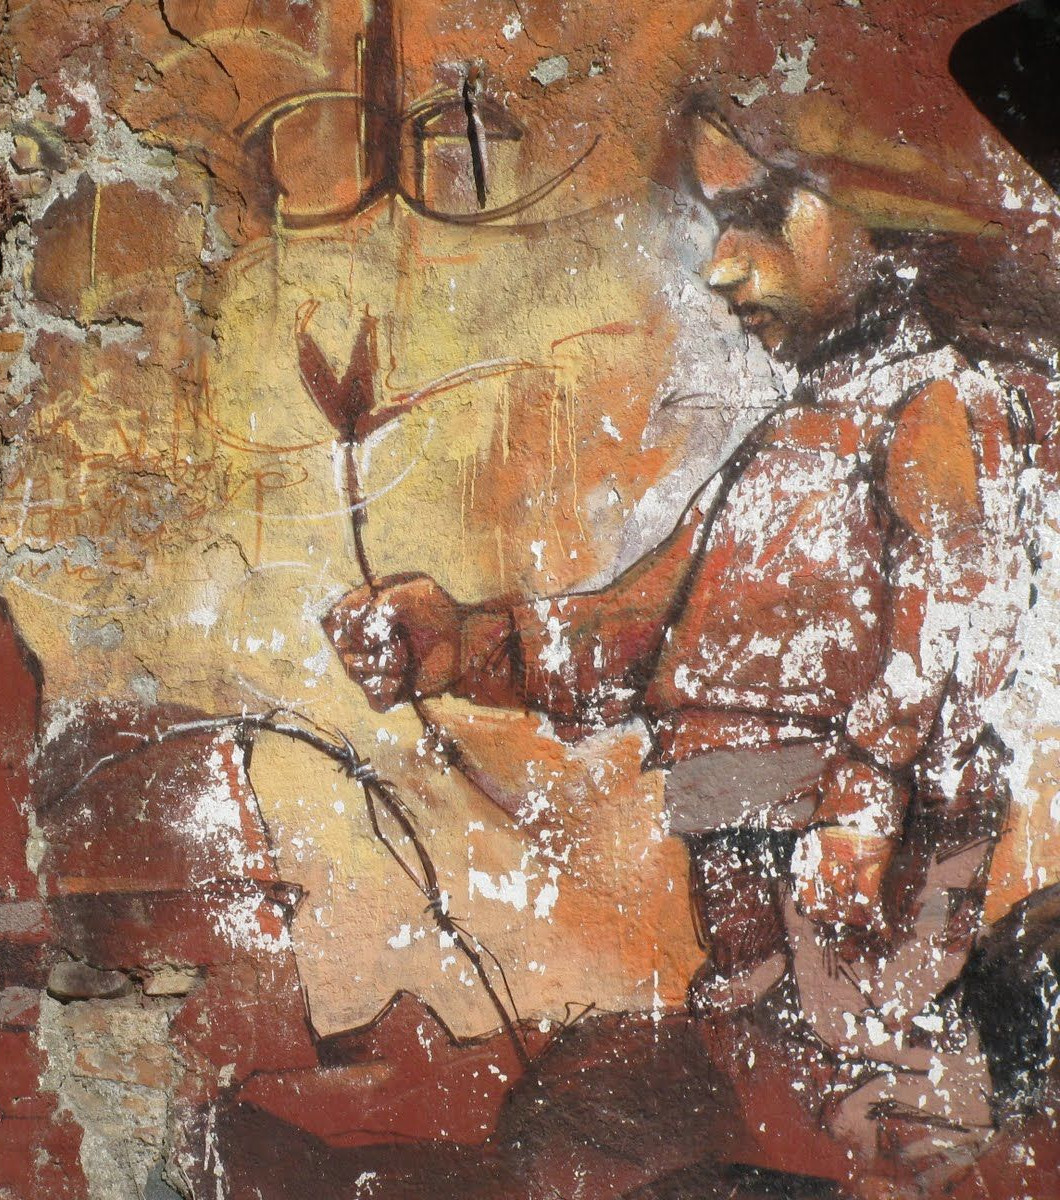
\includegraphics[width=\paperwidth,height=\paperheight]{./Figures/cover/n_pared_2.jpg}};
\tikz[remember picture,overlay] \node[opacity=0.3,inner sep=0pt] at ([yshift=3cm,xshift=2cm]current page.center){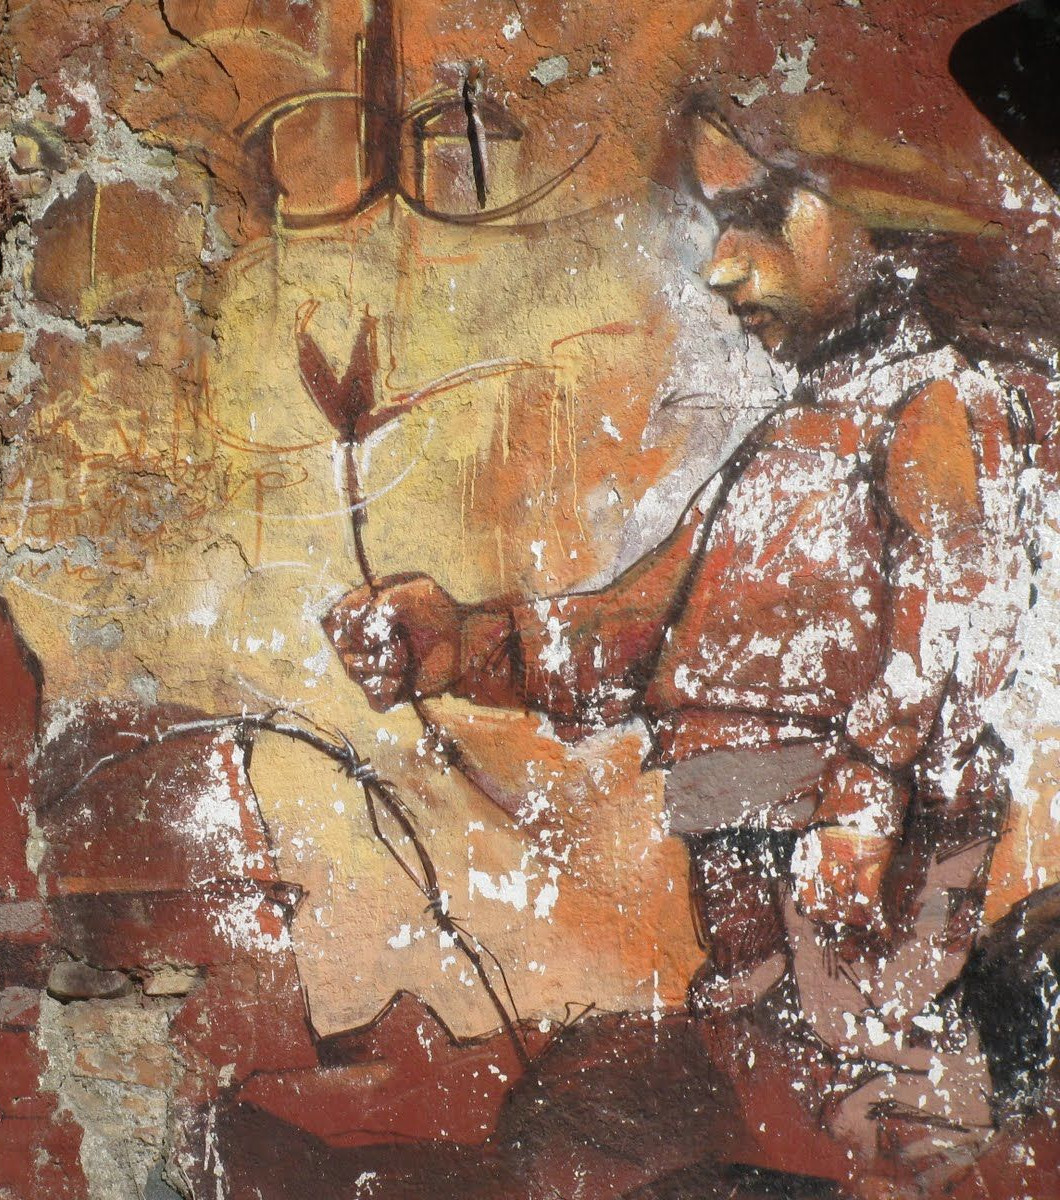
\includegraphics[width=\paperwidth,height=\paperheight]{./Figures/cover/n_pared_2.jpg}};
\clearpage

\section*{Abstract}
No species can persist in isolation from other species, but how biotic interactions affect species persistence is still a matter of inquiry. Is persistence more likely in communities with higher proportion of competing species, or in communities with more positive interactions? How do different components of community structure mediate this relationship? We address these questions using a novel simulation framework that generates realistic communities with varying numbers of species and different proportions of biotic interaction types within and across trophic levels. We show that when communities have fewer species, persistence is more likely if positive interactions—such as mutualism and commensalism—are prevalent. In species-rich communities, the disproportionate effect of positive interactions on persistence is diluted and different combinations of biotic interaction types can coexist without affecting persistence significantly. We present the first theoretical examination of how multiple-interaction networks with varying architectures relate to local species persistence, and provide insight about the underlying causes of stability in communities.

\section{Introduction}

Persistence of multicellular organisms depends on interactions with other organisms, whether they be in the form of energy intake, use of habitats created by other species, assistance in reproduction by directed dispersal of genetic material, or countless other examples \citep{Bascompte2007}. Ecological communities can be represented as networks, whereby species or guilds are nodes connected by links representing interactions \citep{Proulx2005}. Pairwise direct interactions can have positive, negative or neutral effects on the species involved, and this classification gives rise to five general types of interactions: amensalism (-,0), antagonism (+,-), commensalism (+,0), competition (-,-) and mutualism (+,+). Despite the wealth of empirical observations of biological interactions in nature, there still exists limited understanding of the frequency with which different types of biotic interactions occur in communities, and the consequences for community structure and functioning. For example, is the frequency of interaction types in communities related to overall persistence of species locally? Does the structure of the different interaction types play a role in increasing the odds of species persistence? Answering these and other questions has been hampered by difficulties in simultaneously sampling different interaction types in natural systems. Consequently, most studies have been based on observations of single interaction types within networks, which obviously has limited the ability to generalize beyond particular cases.

This fundamental gap in the understanding of ecological networks has been largely acknowledged \citep{Strauss2004, Agrawal2007, Ings2009, Fontaine2011}, and there is increasing evidence that accounting for different interaction types generates novel insights on the structure and dynamics of ecological communities \citep{Pilosof2017, Garcia-Callejas2018}.  Analyses of networks with multiple interaction types have already been applied, for example, to investigate the distribution of the different interaction types and its relationship with species traits \citep{Kefi2015,Kefi2016a} or the robustness of communities to local extinctions and habitat loss \citep{Pocock2012,Evans2013a}. Recent studies have also focused on investigating the relationship between the diversity of interaction types and several facets of community stability, often reaching different conclusions over this relationship. For example, it has been proposed that 1) mixing of interaction types generally increases local stability of model communities \citep{Mougi2012,Mougi2014,Kondoh2015}, 2) mixing of interaction types generally decreases local stability of model communities or increases the number of functional extinctions \citep{Suweis2014,Sellman2016}, or 3) structural factors of the different sub-networks enhance or decrease their stability \citep{Melian2009,Sauve2014,Sauve2016}. The conflicting results over this fundamental question can be explained by the sheer diversity of modeling assumptions, structural constraints, and varying sets of interaction types included in the studies. For example, several studies \citep{Melian2009,Sauve2014,Sauve2016} analyzed communities consisting of only antagonistic and mutualistic interactions in which a central group of species (usually plants) is the guild connecting the mutualistic (e.g. plant-pollinator) and antagonistic (e.g. plant-herbivore) networks. Other studies considered model communities with only basic rules about food web structure \citep{Mougi2012,Suweis2014}. A common feature of most studies is that, with the exception of \cite{Mougi2016a}, their models did not consider the five general interaction types concurrently. However, \cite{Mougi2016a} only analyzed random interaction matrices in his model, making his conclusions difficult to contrast with those of other studies that assumed stronger structural constraints. The role of species richness in mediating community stability also has been extensively studied in single-interaction networks, and analytical derivations have been produced for idealized conditions in mutualism-competitition networks \citep{Allesina2012}. In most cases, theory shows that increasing richness decreases local stability of random networks, but it is unclear how species richness mediates different facets of stability in networks with more complex structures and varying proportions of interaction types.

All in all, while approaches assessing the local stability of random interaction networks have important heuristic value \citep{Allesina2012,Allesina2015}, such randomly assembled networks lack key structural patterns found in real communities \citep{Jacquet2016}. Furthermore, local stability analyses have little concordance with non-equilibrium dynamics of real systems \citep{Pimm1982,Chen2001}, which limits their predictive ability. The equilibrium assumption is further ingrained in most interaction models by assuming that interactions occur with a constant strength coefficient. This assumption is widely used for convenience despite repeated claims against its realism \citep{Abrams1980,Abrams2001,Hernandez1998,Holland2009}. Here we address all the above-mentioned shortcomings and investigate whether the frequencies of the five biotic interaction types affect persistence of species in communities with varying species richness. We generate model networks informed by empirical observations on distributions of species abundances across trophic levels, link topology, and develop a measure of the impact that a species has over another based not on static interaction coefficients, but on species abundances and their associated frequency of interaction. With this model design, and by performing a comprehensive set of simulations, we ask the following questions: 1) Is species persistence affected by the frequency of the different interaction types in model communities? If so, does community richness mediate this relationship? 2) Which types of biotic interactions are more likely to be lost, as species go locally extinct? Lastly, given the unfeasibility of validating our predictions with empirical data, we indirectly test the validity of our model by asking: 3) does our model generates community-level patterns consistent with those of empirical networks?

\section{Methods}

We designed a dynamic network model accounting for the five possible types of pairwise interactions (antagonism, amensalism, commensalism, competition, and mutualism), whereby the impact of a species over another is characterized by the abundances of the species involved. Accounting for different interaction types meant that a trophic level distribution of species had to be specified a priori, as we expected different interaction types to be distributed unevenly across trophic levels. Furthermore, the modeling of pairwise interactions in our model is closely linked to the abundances of the interacting species, so we imposed non-random initial abundance values. In particular, we assembled our model communities with three assumptions:

1) The initial Species Abundance Distribution of the overall community follows a hollow curve.


2) The initial abundances of the different trophic levels vary with a power-law scaling.


3) The distribution of interaction types within and across trophic levels is non-random.


In the following sections, we describe these assumptions and the methodology for incorporating them in the community assembly process. Then, we specify the implementation of the dynamic interactions model and the simulations performed. The main response variable obtained from our simulations is the ratio of persistent species in our model networks. Thus, in the context of the present study, we define community persistence as the ratio between initial (denominator) and final (numerator) number of species in a simulated community. Persistence values can therefore range from 0 (all initial species have died out by the end of the simulation) to 1 (all species show positive abundances at the end of the simulation).

\subsection*{1) Abundance distribution of the overall community}

Each species within a model community was assigned an initial abundance by drawing random samples from a gambin distribution. The gambin is a distribution with a single free parameter that provides a similar or better fit to empirical SADs than classic choices such as the lognormal or the logseries \citep{Matthews2014a}. A value of $\alpha = 2$ was given to generate the initial SADs.

\subsection*{2) Abundance scaling across trophic levels}

Species were distributed among four trophic levels (a basal one consisting on primary producers and three consumer levels), which is a number commonly found in empirical communities \citep{Ulanowicz2014a}. Assignment of species into each trophic level was made following the findings of \cite{Hatton2015}, who showed that for herbivore-predator trophic guilds, biomass distribution follows a power law with exponent ~ 0.75. These authors generalized the scaling rule to the abundance of species at each trophic level since, for most predator-prey couplings, weak relationships between body mass and community biomass were found. As a starting working hypothesis for the simulations, we extended Hatton’s et al (2015) scaling rule to the four trophic levels considered.

\subsection*{3) Distribution of interaction types within communities }

The different types of biotic interactions are unlikely to be uniformly distributed in nature. Yet little is known regarding the varying proportion of interaction types within communities or trophic levels \citep{Dodds1997}, let alone about changes in such proportions across communities, or the effects of varying proportions of interaction types on mechanisms of community assembly.

A first step towards examining the frequency distribution of the different interaction types in a community with several discrete trophic levels is to consider the sign matrix of the community, $S$, assuming that interaction signs are kept constant within the spatial and temporal limits of the study, and with varying abundances. We hypothesize that the relative frequency of each interaction type in S will be influenced by the number of species in the different trophic levels, as different interaction types will have different probabilities of occurring among species belonging to the same or different trophic levels. In order to check this working hypothesis, we undertook an extensive survey of literature on biotic interactions and compiled the extent to which the five general interaction types (amensalism, antagonism, commensalism, competition, mutualism) are documented to occur between species of the same, adjacent, or non-adjacent trophic levels. Specifically, we performed a search in the Web of Science for studies published from 1991 to 2015, including the terms “ecology” AND “interaction” AND “interaction type” (see also \citealt{Morales-Castilla2015}). We reviewed studies documenting direct pairwise interactions and annotated the trophic level of the species involved. For competition, antagonism (predation OR herbivory), and mutualism, we included \textit{ca}. 100 papers. For commensalism and amensalism the list of suitable studies was more reduced (67 studies on commensalism and only 12 on amensalism). We constrained the results by discarding interactions involving microorganisms, fungi, parasites or parasitoids, owing to the overall difficulty of classifying these groups into clear cut trophic levels. The list of selected studies is available as online supplementary material in the published article, see section \textit{Chapter references} for the full reference. The resulting relative frequencies (Fig. \ref{fig:fig3.1}) were incorporated as a last constraint in the model in the form of probabilities of pairwise interactions taking place within a single trophic level, adjacent, or other trophic levels.

For estimating the number of links of each species, we followed the constant connectance hypothesis \citep{Martinez1992}. Thus, we assumed no variation in connectance levels with initial community size, imposing C = 0.5 for every simulation, where connectance is defined as the ratio between realized and potential interactions in the network. This value was chosen so that specific connectances of the different interaction types (see Appendix 3.4) ranged between 0.07 and 0.2, values consistent with empirical estimates of mutualistic and antagonistic connectance \citep{Thebault2010}.

With the probabilities of interaction occurrence across trophic levels (Fig. \ref{fig:fig3.1}) and connectance values of the network, we constructed the sign matrices of our model communities stochastically: for each link, first its interaction type is selected; second, the trophic levels affected by that interaction are chosen according to the probabilities of interaction occurrence; and third, the specific species are randomly chosen. This process ensures that, on average, sign matrices will reflect the probabilities of Fig. \ref{fig:fig3.1}, while allowing for an intrinsic component of variability in each particular matrix. The full community assembly process is explained in detail in Appendix 3.1.

\begin{figure}[!ht]
\centering
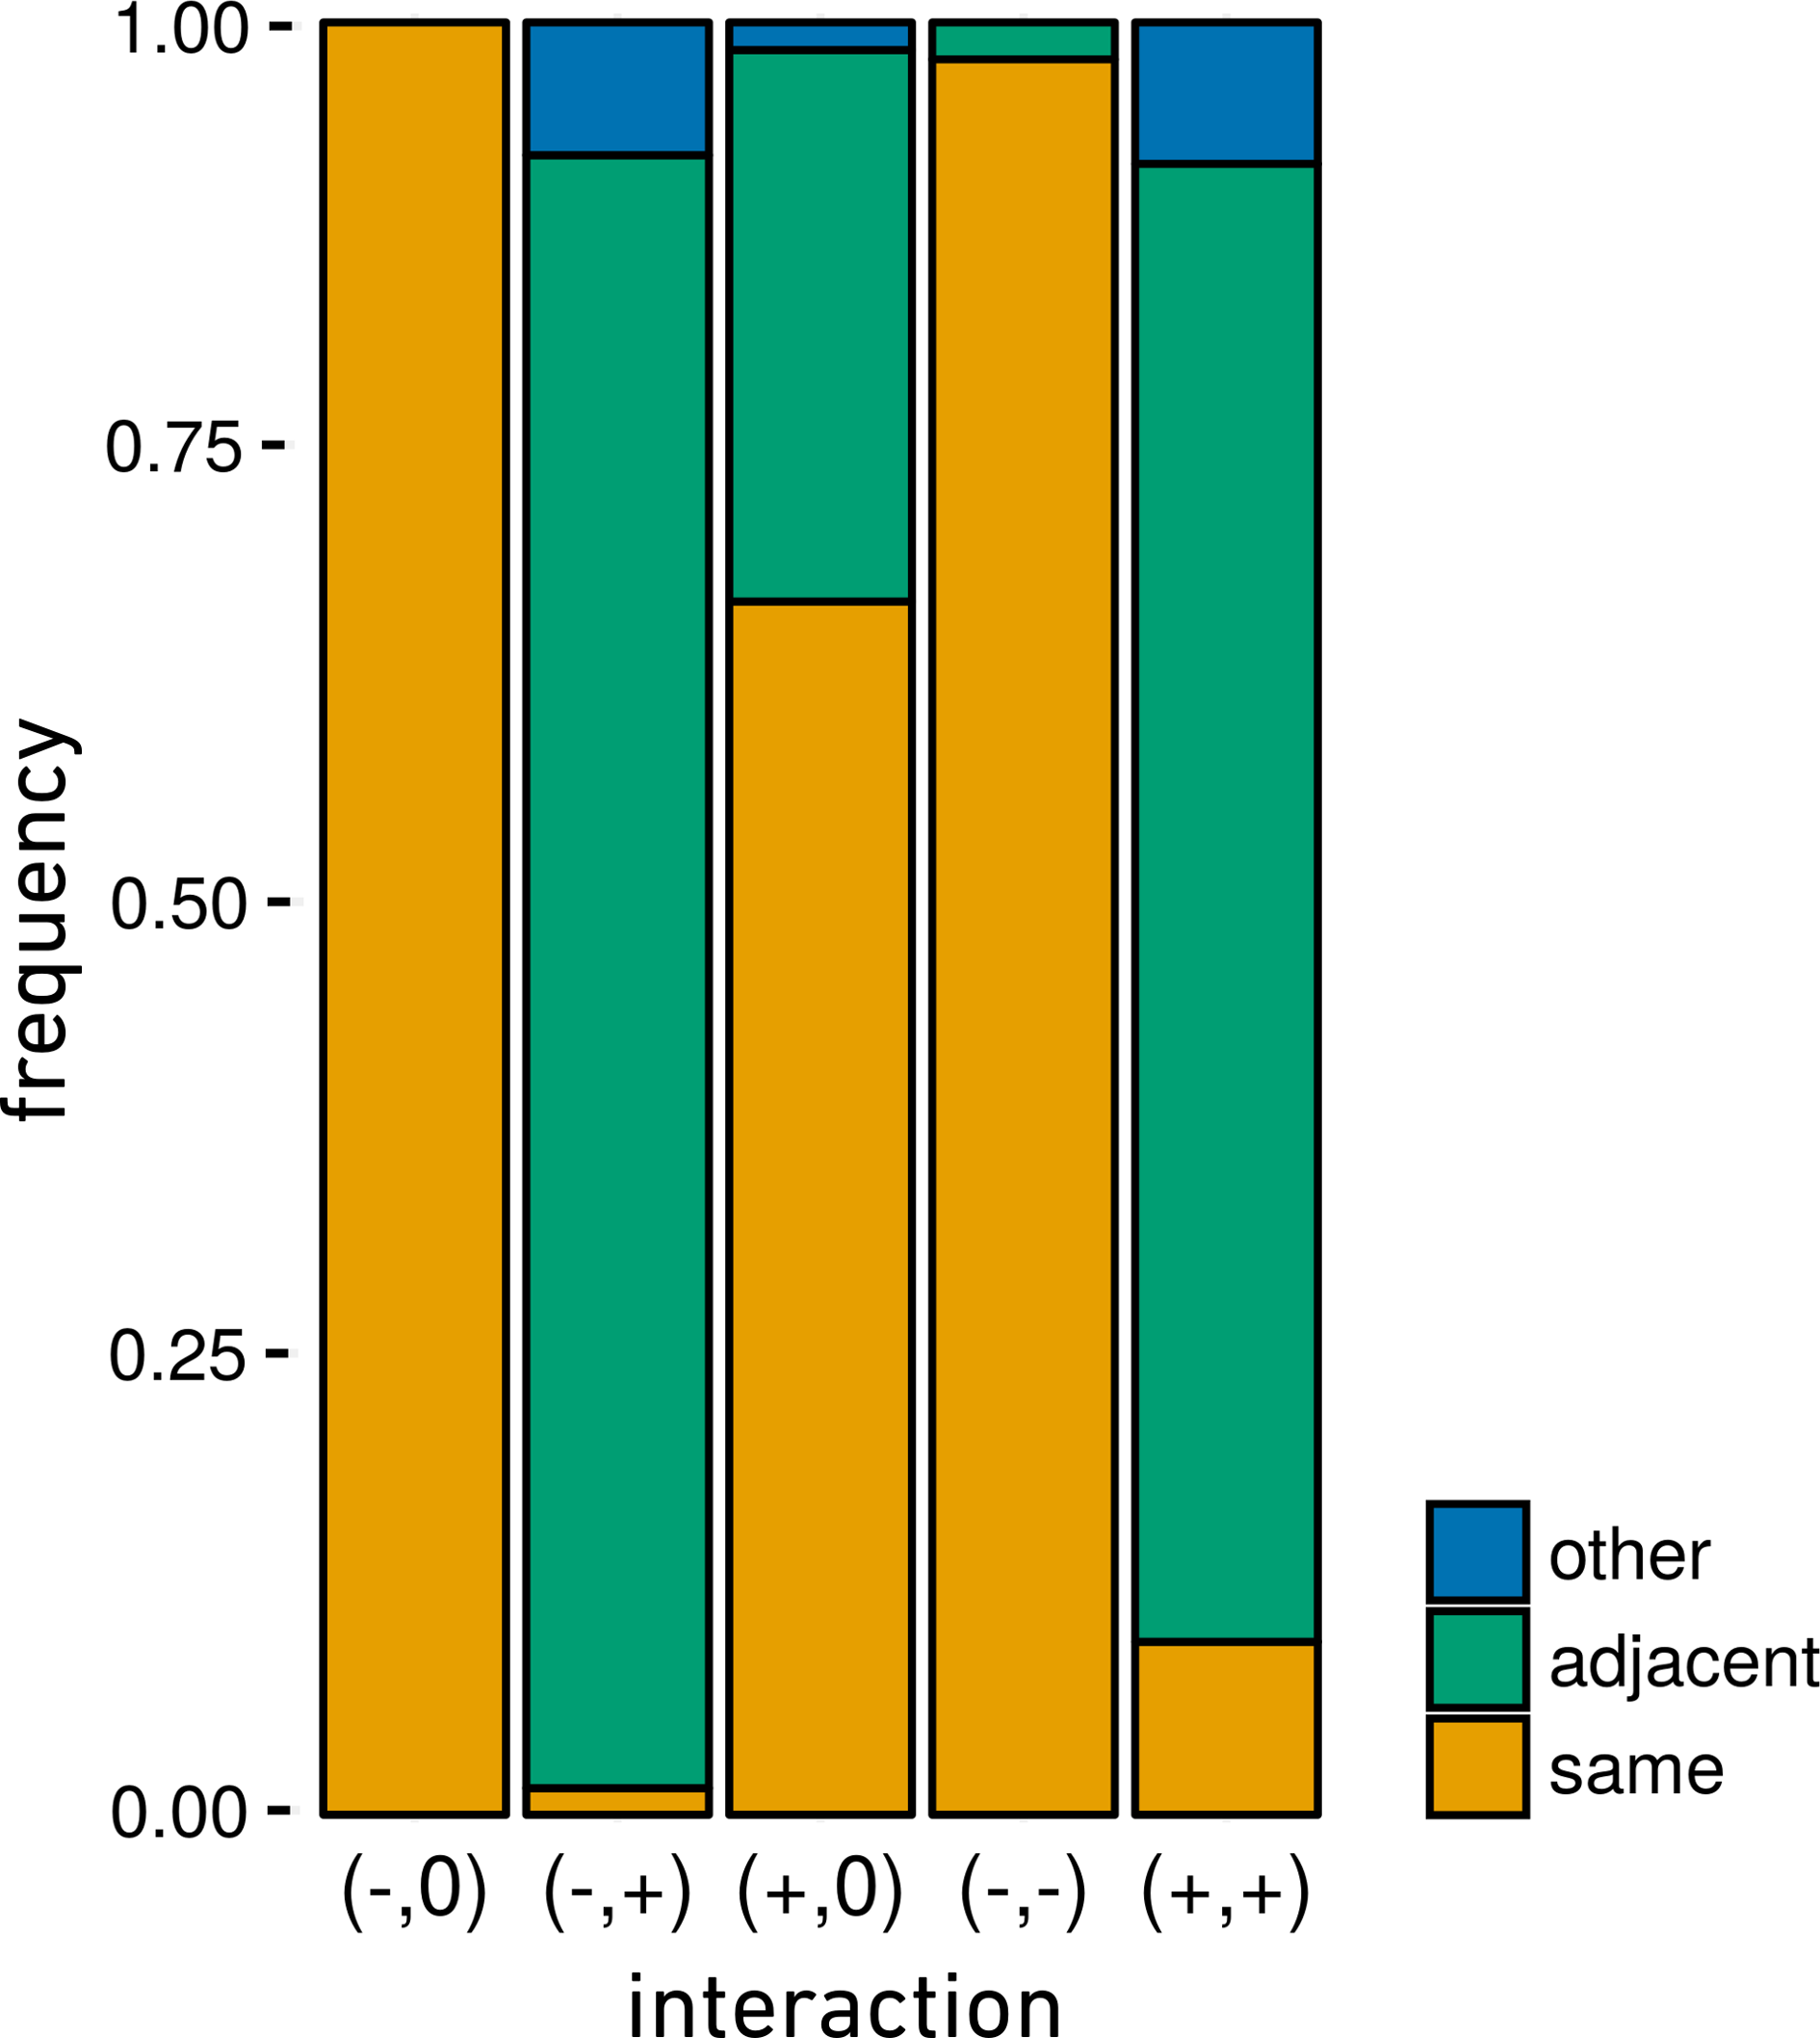
\includegraphics[width=.5\textwidth]{./Figures/chapter03/Fig_1.png}
\caption[Interaction occurrences across trophic levels]{\color{Gray} relative frequency of trophic levels involved in pairwise interactions for each interaction type. When the trophic level of the interacting species was not explicitly alluded to, we assumed that 1) species of the same taxonomic group belong to the same trophic level (e.g. isopods), 2) omnivory represents feeding on both “adjacent” and “other” trophic levels, 3) pollinators and seed dispersers are “adjacent” to plants. $N_{amensalism} = 12$, $N_{antagonism} = 135$ (123 of adjacent trophic levels, 10 of other, 2 of same), $N_{commensalism} = 65$ (44 of same trophic level, 20 of adjacent, 1 of other), $N_{competition} = 97$ (95 of same trophic level, 2 of adjacent), $N_{mutualism} = 113$ (94 of adjacent trophic levels, 11 of same, 9 of other).}
\label{fig:fig3.1}
\end{figure}

\subsection*{A framework for modeling dynamic interactions}

The realization and outcome of direct pairwise interactions is dependent on three classes of mechanisms \citep{Poisot2015}: First, the frequency of stochastic encounters of individuals mediated by their relative abundances. Second, the matching of traits between individuals that establish contact. Third, other factors such as environmental constraints or the influence of higher order interactions with other species. Hence, empirical measurements of interactions show a high degree of variability explained, partly, by density-dependent mechanisms \citep{Aizen2014}, by trait matching \citep{Santamaria2007} or by environmental factors \citep{Mazia2016,Poisot2017}. This inherent variability on both the sign and the strength of interactions has hardly been explored in community dynamic models, even if the assumption of static interaction sign and strength is known to be unrealistic \citep{Abrams1980,Abrams2001,Hernandez1998,Holland2009}. The importance of each mechanism in explaining observed patterns of interaction strengths is currently under debate. In plant-pollinator networks, for example, the net impact of a species over another is significantly related to the frequency of interaction \citep{Vazquez2005,Vazquez2012}, and to the abundances of the interacting species \citep{Vazquez2007}, but not in all cases. A neutral model of interactions can also reproduce structural patterns observed in empirical food webs \citep{Canard2012}. On the other hand, trait-matching has been shown to accurately reproduce network structure in different types of networks \citep{Eklof2013}, and also outperforms neutral interaction frequency for predicting network structure in some empirical networks \citep{Vizentin-Bugoni2014,Sazatornil2016}. However, another recent study showed that while abundances and traits can predict network structural patterns, they were not generally able to predict the realization of specific interactions in a plant-pollinator network \citep{Olito2014}. Finally, higher-order influences on interaction occurrence and strength, in particular environmental forcing, are a main focus of Stress Gradient Theory \citep{Maestre2009} and Environmental Stress Models \citep{Menge1987}, but an integration of these frameworks with the recent advances on multi-trophic, multiple interactions networks is still lacking.

We modeled the impact of a species over another by considering the first of these three mechanisms, i.e. the stochastic encounters between individuals of two populations driven by their abundances. This process is the only one that can be generalized to any interaction and community type without considering further, specific assumptions about trait distributions or the role of environmental covariates. Thus, in our modeling framework, the impact of a species over another is only dependent on the frequency of interaction between the two species, which in turn depends on their net abundances. As our approach is fundamentally different to that of models with static interaction strength coefficients, we refer to the interaction strength in our model as species impact (a population-level effect, \citealt{Vazquez2012}).

In formulating species impact, we followed \cite{Poisot2015} and considered it a product of interaction frequency by an interaction strength term:

\begin{equation} \label{eq:eq3.1}
I_{i,j} = IF_{i,j} * IS_{i,j}
\end{equation}

The $IF$ function derives the net frequency of interactions between two populations in a given time interval from their local abundances. We assume that (1) the maximum potential interaction frequency will equal the population density of the least abundant species, and (2) interaction frequency saturates asymptotically, as one or both abundances increase. It takes the form:

\begin{equation} \label{eq:eq3.2}
IF_{i,j} = min(N_i,N_j) \frac{1}{1 + e^{-a(max(N_{i},N_{j}) - x_0)}}
\end{equation}

The $a$ parameter adjusts the saturating behavior of the function (i.e. its steepness), so that a higher value of a implies that the $IF$ function saturates at lower abundances of both populations, i.e. interactions are comparatively more common. Parameter $x0$ indicates the abscissa of the midpoint for the logistic part of the function, and was kept for reference.

The $IS$ function (for interaction strength) models the sign and strength of per capita interactions of species $j$ over species $i$. This function was defined just as the sign of the pairwise interaction times a scaling factor for differentiating interaction types. For example, a scaling of 1 indicates that the maximum effect of species $j$ over species $i$ is of the same order of magnitude as the population growth rate. Therefore, we defined the $IS$ function simply as:

\begin{equation} \label{eq:eq3.3}
IS_{i,j} = s_{i,j} * k_t
\end{equation}

where $s_{i,j}$ is the sign of the effect of species $j$ over species $i$, and $k_t$ is the scaling factor for an interaction of type $t$.

We incorporated Eq. \ref{eq:eq3.1} to a population dynamics model based on the recent extensions to the logistic growth equation by \cite{Garcia-Algarra2014}. Their formulation averts a known divergent behavior of the r-k classic form of the logistic equation and is sufficiently simple while being able to reproduce the complexity of more elaborate models in terms of fixed points and stabillity of the dynamics. Consider a community of $n$ species. The model has the form:

\begin{equation} \label{eq:eq3.4}
\frac{dN_i}{dt} = r_i N_i
\end{equation}

whereby all extrinsic effects – environmental, biotic interactions – fall on the intrinsic growth rate $r_i$. This allows the comparison between the strength of different interactions, i.e. it is an example of an equal footing network \citep{Garcia-Callejas2018}. The effective growth rate is modeled as:

\begin{equation} \label{eq:eq3.5}
r_i=r_i^0+\sum_{j=1,j{\neq}i}^n I_{i,j} - (\alpha_i + c_i \sum_{j=1,j{\neq}i}^{n} I_{i,j})N_i
\end{equation}

where $r_{i}^{0}$ is the intrinsic growth rate, $\alpha_i$ is the friction term that regulates the asymptotic behavior of the function, $c_i$ is a proportionality constant, and $I_{i,j}$ is the impact function from Eq. \ref{eq:eq3.1}.

\subsection*{Simulations}

We generated theoretical communities with 20,40, and 60 initial numbers of species that corresponded to overall abundances of around 2395, 4640 and 6850 individuals, respectively. For each richness level, we defined six types of communities according to the frequency with which the different interaction types occurred: equal ratio type with relative frequency of 0.2 for every interaction type; and five types in which each of the interaction types was the most prevalent (with frequencies of 0.4 for the prevalent type and 0.15 for the others). We projected the dynamics of 1000 replicates for each of these combination of factors, ending up with $3*6*1000 = 18000$ simulated communities. For each replicate, aside from the inherent stochasticity of the assembly process, we drew the intrinsic growth rates and saturation terms of each species ($r_{i}^{0}$ and $\alpha_i$ from eq. \ref{eq:eq3.5}) randomly from an interval of potential values (Appendix A.3.1: Table A.3.1.4), ensuring that primary producers have intrinsic growth rates $r_{i}^{0} > 0$ and consumers $r_{i}^{0} < 0$. Introducing these stochastic components on the assembly process and parameterization enabled us to test the robustness of the model to small variations in its initial conditions. The full parameterization of the model, alongside with further details about its implementation and numerical solving, is given in Appendix 3.1. Preliminary tests showed that most simulated communities reached a stable abundance distribution after 2500 or less time steps but, conservatively, we ran our dynamic model for 5000 time steps. In order to be more confident on the time steps chosen, we also tested whether there were significant differences between the resulting persistence patterns after 5000 and 10000 time steps. As no significant differences were found, we considered 5000 time steps to be an appropriate time frame for our simulations.

We also performed additional simulations in order to test the influence of the imposed structural constraints in our results. In these simulations we relaxed, one by one, the three constraints of the community assembly process (see Appendix 3.3 for more details).

\section{Results}

\subsection*{Is species persistence influenced by the frequency of the different interaction types? If so, does community richness mediate this relationship? }

Model communities with a higher proportion of positive interactions (mutualism and, to a lesser extent, commensalism) tended to have higher species persistence than any other community type (Fig. \ref{fig:fig3.2}, results of statistical tests in Appendix A.3.2: Table A.3.2.1 and Table A.3.2.2). The effect of positive interactions on persistence was strongest for species-poor communities, and decreased consistently as the numbers of species in the communities increased. Although average species persistence converged to around 88\% as richness increased, there was significant variation between the persistence of species belonging to the different trophic levels (Appendix A.3.2: Figure A.3.2.1): in communities with low initial richness, the second and third trophic levels saw more extinctions than the first, while species on the fourth trophic level did not show a uniform behavior, and were more dependent on variations in the relative frequency of interaction types. This general pattern was reversed in more speciose communities, in which species of all higher trophic levels showed more persistence than the basal ones, for all community types.

Supplementary simulations (Appendix A.3.3) showed that persistence values are further influenced by the community structural patterns imposed. The removal of both the abundance scaling across trophic levels and the distribution of interaction types across trophic levels had a significant negative effect on persistence. Sampling species abundances from a uniform SAD instead of a skewed one, on the other hand, increased overall persistence.

\begin{figure}[!ht]
\centering
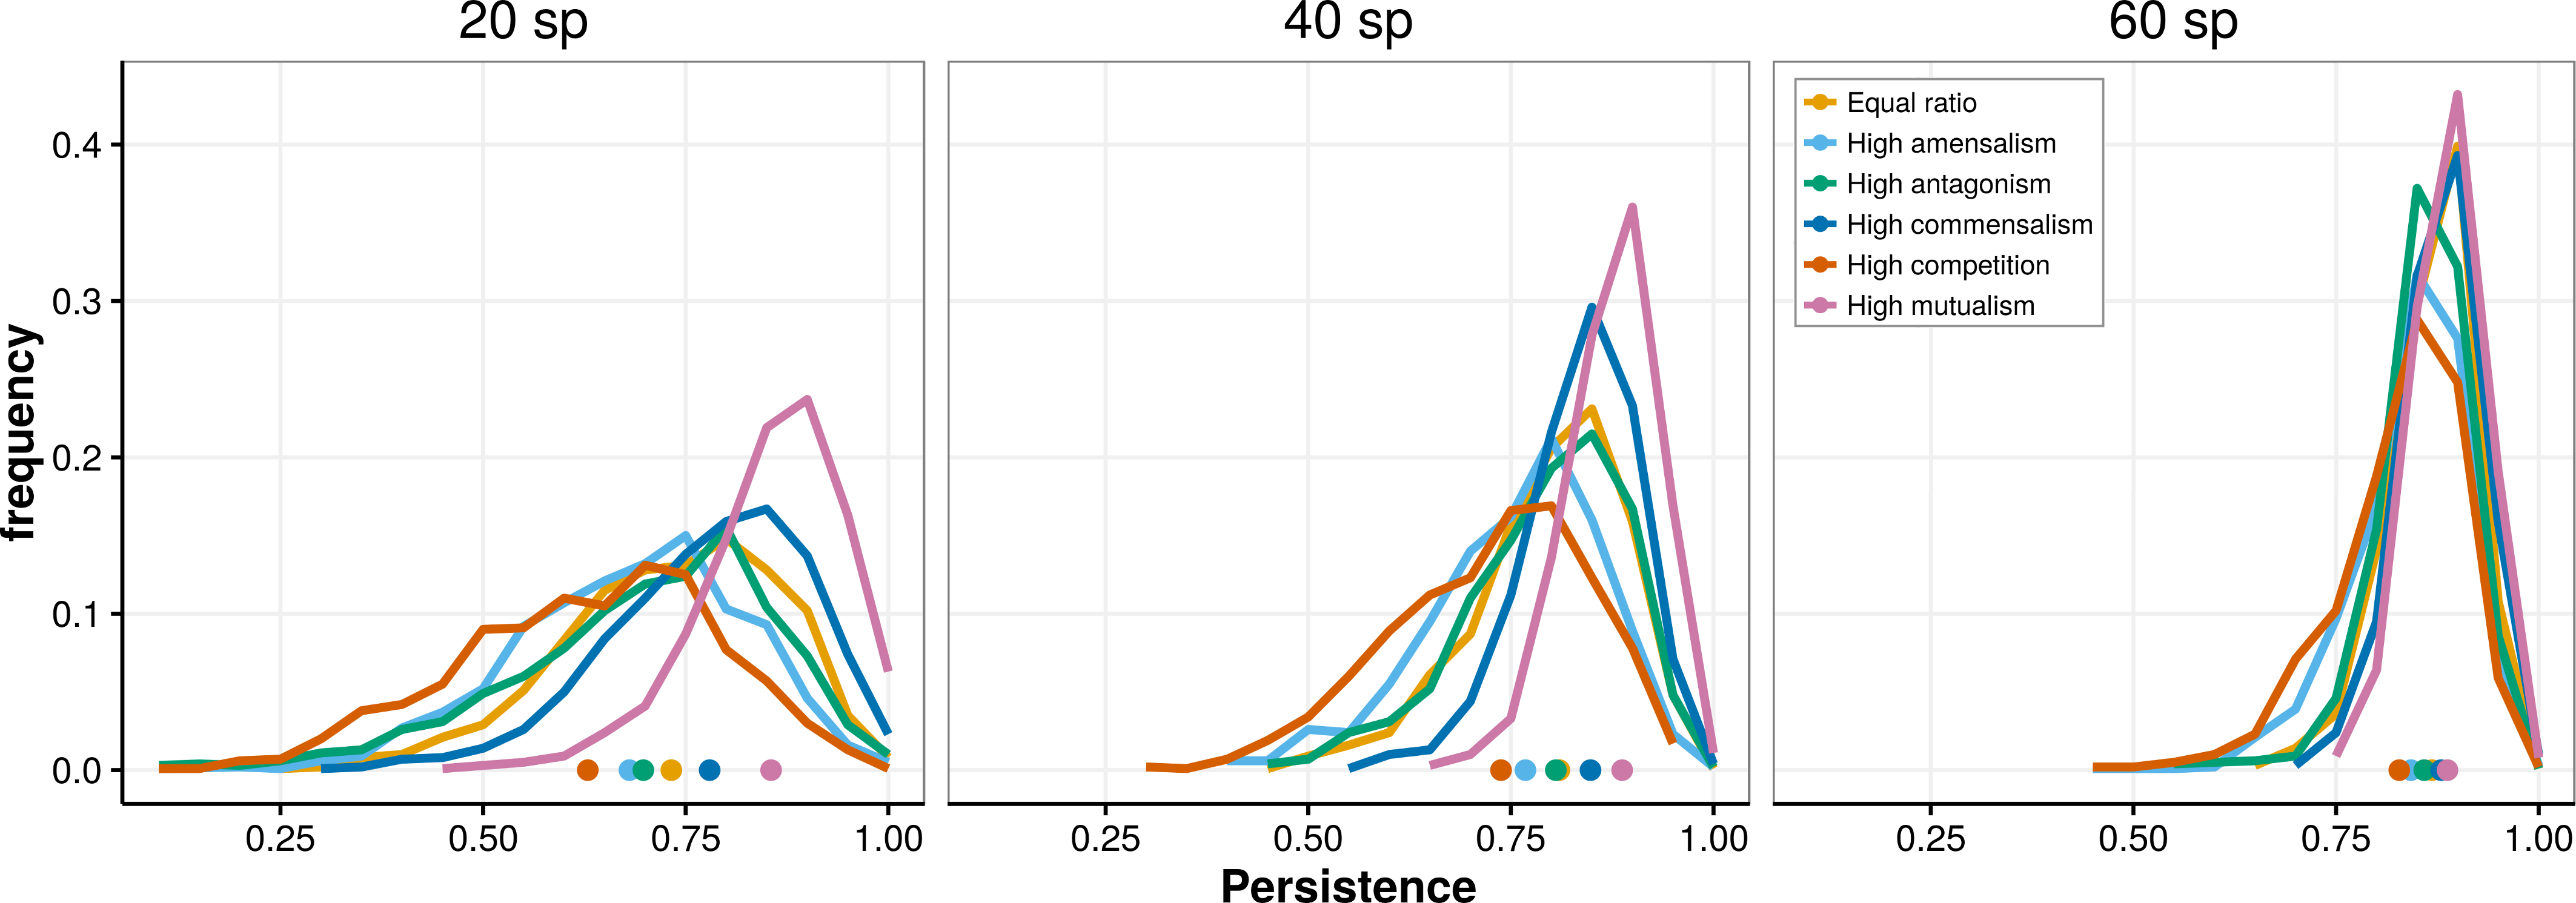
\includegraphics[width=\textwidth]{./Figures/chapter03/Fig_2.png}
\caption[Persistence of model communities]{\color{Gray} Persistence values of the simulated communities at the end of the simulations. Vertical axis represents the relative frequency of a given persistence value in the pool of replicates (1000 replicates for every combination of initial richness and initial frequency of interaction types). All resulting pairs of persistence distributions but one are significantly different according to Kruskal-Wallis rank tests (Appendix A.3.2: Table A.3.2.1) and post-hoc Dunn’s tests (Appendix A.3.2: Table A.3.2.2).}
\label{fig:fig3.2}
\end{figure}

\FloatBarrier

\subsection*{Which types of biotic interactions are more likely to be lost, as species go extinct?}

In our model, local extinctions have structural consequences for the remaining network: when a species goes extinct, its interactions disappear as well and are not replaced. The initial and final frequencies of the different interaction types were significantly different in most cases (Fig. \ref{fig:fig3.3}, results of statistical tests in Appendix A.3.2: Table A.3.2.3). Amensalism and competition tended to decrease in relative frequency with respect to initial levels, while mutualism tended to increase. Antagonism and commensalism responded differently for varying levels of community richness. Antagonistic interactions decreased in frequency only in communities with 20 initial species, while in communities with 60 species, they increased; the opposite was observed for commensalism, which increased in species-poor communities but decreased with high species richness.

\begin{figure}[!ht]
\centering
\includegraphics[width=\textwidth]{./Figures/chapter03/Fig_3.png}
\caption[Initial and final interaction ratios]{\color{Gray} Initial and final frequency of each interaction type in each community parameterization (rows: richness levels, columns: interaction frequencies levels). Each dot represents a single simulation, color code is the same as Fig. \ref{fig:fig3.2}. Upper left symbols in each panel represent the significance of the difference in initial and final ratios according to Wilcoxon signed rank paired tests, in black for the whole set of simulations, and colored for the simulations with high ratio of the respective type (n.s.: p-value > 0.05, *: p-value $<$ 0.05, **: p-value $<$ 0.01, ***: p-value $<$ 0.001. See Appendix A.3.2: Table A.3.2.3 for details.}
\label{fig:fig3.3}
\end{figure}

\FloatBarrier

\subsection*{Does our model reflect structural patterns observed in empirical networks?}

Focusing on the structural features listed by Jacquet et al. (2016), we checked three features observed in empirical networks: the distribution of interaction strengths (species impacts in our scheme), their variation in magnitude with trophic level, and the correlation of antagonistic pairwise interaction impacts. The distribution of species impacts in our model communities ($I_{i,j}$ in Eq. \ref{eq:eq3.1}) was positively skewed in all cases, with communities with high proportion of negative interactions being the most skewed (Fig. \ref{fig:fig3.4}, Appendix A.3.2: Table A.3.2.4). The magnitude of species impact decreased consistently with increasing trophic level (Fig. \ref{fig:fig3.4}, Appendix A.3.2: Table A.3.2.5 and Table A.3.2.6). Lastly, there was a significant negative correlation in the values of pairwise species impact for antagonistic interactions (Fig. \ref{fig:fig3.4}, Wilcoxon signed-rank tests, $V = 0$, $p < 0.001$ in all cases).

\begin{figure}[!ht]
\centering
\includegraphics[width=\textwidth]{./Figures/chapter03/Fig_4.png}
\caption[Community structural patterns]{\color{Gray} Structural patterns observed in our model, at the initial and final steps of the simulations. Data shown corresponds to simulations with an initial richness of 60 species and equal probability of occurrence for every interaction type. a) Skewed distribution of species impacts. b) Decrease in average impact per trophic level (error bars represent an interval of one standard deviation centered in the mean). c) Correlation of species impact among pairs of species. In this panel, the only interactions accounted for are antagonistic ones.}
\label{fig:fig3.4}
\end{figure}

\section{Discussion}

Our simulations indicate, primarily, that positive interactions are key for maintaining species persistence, particularly in species-poor communities. For understanding the outcomes of our model and in order to place them in a general context, we first evaluate the role and implications of modeling interaction impacts based on species abundances and interaction frequencies. Secondly we analyze the combined influence of other community-level factors.

\subsection*{Species persistence and pairwise direct interactions}

All other things being equal, the number of interactions every species has with other species (i.e., their degree) is expected to increase with increasing number of species in the community. This is exactly what we recorded in our model communities: by keeping network connectance constant, we obtained average degrees of 9.5 for communities of 20 species, and degrees of 19.5 and 29.5 for communities of 40 and 60 species, respectively (values not far from the empirical estimates obtained by \cite{Kefi2015}, who reported an overall connectance of 0.47 for a community of 104 species, and thus a mean overall degree of 24.2). Given such a scenario, in species-poor communities the dynamics of a species will directly depend on only a handful of pairwise interactions. In such cases, a single interaction with high impact will have a disproportionate direct effect on species dynamics and, by extension, the prevalence of negative or positive interaction types will be an important driver of persistence at the community level.

The direct impact of interactions in communities is not only dependent on their numbers, but also on the abundances of the interacting species. Considering a skewed SAD (Species Abundance Distribution) of the overall community, as in our main simulations, the percentage of rare species (e.g. these with $<$ 10 individuals) increases and then stabilizes with increasing richness, while the percentage of very abundant species (e.g. with > 100 individuals) decreases (Appendix A.3.2: Table A.3.2.7). In species-poor communities, thus, a higher proportion of interactions will involve very abundant species, increasing the probability of comparatively strong direct impacts on species dynamics. As richness increases, more interactions will take place between comparatively rare species. The average impact per interaction will decrease accordingly (Appendix A.3.2: Figure A.3.2.2), with the effect that average persistence will increase regardless of the distribution of interaction types.

An important consequence of the differential effect of interaction types on species persistence is that species engaging in a high number of direct positive interactions will tend to persist and maintain their interactions, whereas species with a high number of direct negative interactions will tend to go extinct more frequently and, thus, their associated interactions will be lost, increasing the overall ratio of positive interactions (Fig. \ref{fig:fig3.3}). This reasoning is, however, contingent on the modeling assumption that there is no interaction rewiring. Keeping in mind this strong assumption, if these results hold, natural assemblages should be filtered to maintain a relatively high ratio of direct positive interactions, in particular in species-poor communities, and species with a high degree of negative interactions will be rare and, in any case, have otherwise strong life-history traits that allow them to persist. Note that, throughout the study, we limit our discussion to the role of direct interactions. The importance of indirect or net effects for understanding community patterns is well established (e.g. \citealt{Montoya2009a}), and the mechanisms proposed here for linking species interactions, abundance and persistence, would be improved by accounting for the role of these higher-order effects. However, in model networks, net effects are commonly analyzed by calculating the negative of the inverse Jacobian matrix \citep{Novak2016}. The formulation of our model, without static interaction coefficients and, potentially without attaining static equilibria, limits the applicability of analyses based on Jacobian matrices. Therefore, we opted not for calculating net effects and leave their analyses in our framework for future studies.

By explicitly modeling species impacts based on species abundances and interaction frequencies, our interpretation of species persistence and community dynamics differs fundamentally from that of other theoretical models of multiple interactions (e.g. \citealt{Mougi2012}). Furthermore, our response factor, species persistence, also differs from the common local stability analyses performed in the majority of theoretical network studies. Despite these fundamental differences, some common trends seem to surface. Much like our finding that the frequency of interaction types is less important in speciose communities, in the study by \cite{Mougi2012} increasing richness allowed for high local stability regardless of the proportion of positive to negative interactions (but see \citealt{Suweis2014}). With a completely different methodology, built on individual-based models, \cite{Lurgi2016} further found that increasing the proportion of mutualistic links increased overall stability in their model. Yet another, more general interaction model showed that positive interactions tend to become dominant in interaction networks as a consequence of spontaneous self-organization \citep{Jain2001}. Overall, these independent lines of evidence point to the combined importance of positive interactions and community size on stability patterns in a broad sense.

The relationship between species richness, abundances and interaction types may shed light on other general questions in community ecology, aside from the comparison with previous theoretical models.

First, in line with empirical findings from plant communities in stressful environments \citep{Soliveres2014, Cavieres2009}, we have shown that a high ratio of positive to negative interactions significantly increases species persistence, particularly in communities with low initial richness. By the explicit consideration of four discrete trophic levels, we show that a preponderance of positive interactions is particularly important for the persistence of intermediate consumers (Appendix A.3.2: Figure A.3.2.1), upper panels). These species are preyed upon by top predators and also subject to competition (both direct as modeled and indirect as a result of resource consumption) and amensalism. Hence, they are potentially the most benefited from engaging in mutualisms with species from adjacent trophic levels. As mutualistic interactions are most prevalent across adjacent trophic levels (Fig. \ref{fig:fig3.1}), intermediate species will be the ones showing a highest degree of these positive interactions. Note that we did not model competition for resources at the basal trophic level, and all our communities included a fourth trophic level of top predators. Thus, these latter species, not subject to predation (aside from a very small probability of intraguild predation, Fig. \ref{fig:fig3.1}), are likely to have a strong top-down influence on the persistence of intermediate species.

Second, our findings contribute to reframing the debate on whether pairwise interactions are stronger in richer communities. On the one hand, the hypothesis of a gradient on pairwise interaction strength with latitude has been generally supported on empirical grounds (\citealt{Schemske2009}, but see \citealt{Moles2016}), but it is unclear whether or how this pattern is affected by the richness of the analyzed communities. On the other hand, we have shown that if interaction impacts are neutral (i.e. driven solely by species abundances), then species impact will generally decrease with increasing richness. This theoretical result has been partially supported in a recent study that found that, on islands whose size granted a certain environmental stability, the strength of competitive and antagonistic interactions decreased with island size and richness \citep{Schoener2016}. Clearly, an array of factors can cause deviations from neutrality in interaction strengths (IS function in eq. \ref{eq:eq3.1}), and hence the neutral interactions hypothesis should be viewed as a baseline for estimating species impacts when no other information is available. Such neutral estimations have already been applied for plant-pollinator networks \citep{Vazquez2012} or in sampling campaigns of multiple interactions networks \citep{Pocock2012}.

\subsection*{Emerging community structure further enhances persistence}

Components of community structure, such as species diversity or different network-level metrics, have been regarded as key factors in previous modeling studies \citep{Sauve2014,Sauve2016}, where accounting for empirically informed values generally enhances stability metrics. Such theoretical results are, however, difficult to validate, since empirical data on communities with varying structural patterns is extremely scarce. As an alternative for testing the adequacy of our model, we analyzed whether our model communities displayed properties comparable to those found in empirical networks. Recently, \cite{Jacquet2016} showed that empirical food webs possess three structural characteristics that clearly differentiate them from random counterparts: first, they display the classic skewed distribution of interaction strengths, whereby there are very few strong interactions and a majority of weak ones \citep{McCann1998}. Secondly, empirical food webs show strong pairwise correlations in interaction strengths, in line with theoretical findings \citep{Tang2014}. Thirdly, interaction strengths are not evenly distributed across trophic levels; rather, average interaction strength tends to decrease with trophic level. In our model, the skewed distribution of species impacts and their “pyramidal” arrangement are observed and maintained throughout the community dynamics (Fig. \ref{fig:fig3.4}, panels A and B). On the other hand, the pairwise correlations generated in our model communities (Fig. \ref{fig:fig3.4}, panel C) are significantly different from zero but smaller than those reported by \cite{Tang2014}. Such disparity may be due to the lack of trait-matching mechanisms in our model, as trait-matching may give rise to increasingly specialized and correlated pairwise interactions \citep{Santamaria2007}.

The three patterns outlined by \cite{Jacquet2016}, i.e. skewed distribution of impacts, pairwise correlations in interaction strength, and decrease of species impacts with increasing trophic level, are already present at the beginning of the simulations (Fig. \ref{fig:fig3.4}), so they arise from the structural constraints of our community assembly process. It is therefore informative to analyze the dynamics of the model without these constraints, namely 1) a skewed Species Abundance Distribution of the overall community, 2) a sublinear scaling of overall abundances with increasing trophic level, and 3) a non-random distribution of links across trophic levels, for each interaction type (Fig. \ref{fig:fig3.1}).

Relaxing these constraints does not modify the main qualitative patterns of our results, i.e. positive interactions and, to a lesser extent, increasing richness, have a positive effect on persistence (Appendix A.3.3: Figure A.3.3.1), but quantitative outcomes vary. The effect of removing the second and third constraints on species persistence is negative, while removing the first constraint has a generally positive effect on persistence. This effect is particularly strong for upper trophic levels, where average persistence varies widely depending on the assembly constraints imposed (Appendix A.3.3: Figure A.3.3.2). These results invite the interpretation that community structure, both in terms of the topology of the different interaction types and the distribution of species abundances across trophic levels, is a key factor for maintaining high levels of persistence. Despite their recorded importance, understanding of these factors in empirical communities is still limited. Further empirical work is needed to evaluate the generality of the abundance scaling law \citep{Hatton2015} for multiple trophic levels and community types, and, importantly, to understand its underlying mechanisms. Regarding the distribution of interaction types, our approach was to assign probabilities of occurrence based in empirical observations. This methodology is biased towards the most studied interaction types (antagonism, competition and mutualism), and towards easily observed organisms and interactions, thereby failing to account for functionally important yet rarely considered organisms, such as microorganisms, parasites or parasitoids. It has been shown, for example, that accounting for parasites when analyzing food webs significantly modifies network structural patterns \citep{Lafferty2006}, so the interaction probabilities obtained here should be taken as broad estimates. Despite these shortcomings, evidence is increasing theoretically and empirically that link topology is key not only for consumer-resource, but for all interaction types \citep{Pocock2012,Evans2013a,Kefi2015,Kefi2016a,Sauve2016}. Due to the difficulty in obtaining reliable estimates of multiple interactions at once in empirical communities \citep{Garcia-Callejas2018}, we currently do not know whether the distribution and topology of interaction types is homogeneous across communities or how it is influenced by habitat type or environmental factors.

The significant variation in persistence ratios with structural patterns shown here suggests that theoretical studies relying on idealized communities (e.g. totally mixed interactions and/or random distributions of biomass across trophic guilds) are likely to miss key mechanisms for maintaining species persistence. Rather, future studies on multiple interactions networks should take into account the variability of community-level factors present in natural assemblages, like interaction frequencies and distribution, or abundance scalings across trophic levels. Our model is a first step in that direction, but it is important to note that the insights obtained are, of course, contingent on the assumptions made. In particular, important features of the model are the constant connectance hypothesis and the implementation of dynamic interaction impacts. Furthermore, we assumed that the degree of a species is independent of its relative abundance in the community. While none of these assumptions hold completely true in nature, they represent convenient starting hypotheses for modeling complex ecological communities, because ecological interpretations can be drawn when empirical systems deviate from these assumptions \citep{Banasek-Richter2009}. Further investigation on the differential functional form of the different interaction types, e.g. as outlined for mutualism by \cite{Holland2002}, and on interaction rewiring \citep{Valdovinos2010,Mougi2016b}, will also help refine the conclusions obtained here. Aside from these potential developments, our results can be used to establish baseline predictions on the dynamics of natural communities across gradients of richness or other factors. In that regard, the sensitivity of species-poor communities to interaction diversity is of particular interest: as these communities are particularly endangered by anthropogenic drivers of ecosystem change \citep{Cavieres2009}, it is paramount to evaluate this theoretical result and its potential consequences for management and conservation schemes.

\section{Conclusions}

To understand how the persistence of species is influenced by the complex networks of interactions in which they are inserted, it is important to develop models that account for the diversity of interactions present in nature, and that incorporate realistic constraints to the structure of these networks. By developing one of such models, we found that species' local persistence is not explained by a single axis of variation in network properties, but rather is contingent on the interaction of several structural factors: the diversity and distribution of biotic interactions, the size of the community, and the distribution of species abundances across trophic levels. In particular, we found that a high prevalence of positive interactions can lead to increased persistence of species in communities with low richness, whereas speciose communities can sustain varying ratios of interaction types without significant decreases in average persistence. Although simulation studies are, by definition, affected by a number of simplifying assumptions, we found that our simulated networks have emerging features also present in empirical networks, suggesting that our modeling framework captures part of the mechanisms that maintain the richness and diversity of natural assemblages. The insights from network models, such as ours, are one of the complementary ways in which ecologists approach the understanding of local species persistence, and should prove valuable in developing a robust predictive framework for its variation across different types of gradients.

%************************************************
\chapter[Species Abundance Distributions and trophic structure]{On the variability of Species Abundance Distributions with trophic guild and community structure}\label{ch:SAD}
%************************************************

%\tikz[remember picture,overlay] \node[opacity=0.3,inner sep=0pt] at (current page.center){\includegraphics[width=\paperwidth,height=\paperheight]{./Figures/cover/barco_oceano.png}};
\tikz[remember picture,overlay] \node[opacity=0.3,inner sep=0pt] at ([yshift=3cm,xshift=2cm]current page.center){\includegraphics[width=\paperwidth,height=\paperheight]{./Figures/cover/barco_oceano.png}};
\clearpage

\section*{Abstract}

Species Abundance Distributions (SADs) are one of the strongest generalizations in community ecology, but their variation across trophic levels remains largely unexplored. I study the variation in SAD metrics across trophic guilds, using a theoretical model and a compilation of empirical datasets. First, I develop a model that allows tracking the variations in abundances across trophic guilds, controlling for species richness and network connectance. The theoretical results show that evenness is highest for herbivores, and decreases in omnivore and carnivore guilds. The richness and connectance of the community network are also negatively correlated with guild evenness. Second, I compare the empirical SADs of 226 terrestrial plant communities and 497 mammal communities comprising species grouped in three general trophic guilds (herbivores, omnivores, and carnivores). Sampled plant communities are significantly less even and more skewed than mammal ones. There are no significant differences in SAD metrics between the different mammal guilds, but carnivores are comparatively rare (i.e. have a higher proportion of species than individuals), whereas omnivores are comparatively more common. Species richness has a positive effect on both evenness and skewness, and spatial and temporal extent have negative effects on evenness and do not affect skewness. I argue that the difference between plant and mammal guilds can be related to higher niche availability in animals than in plants, that decreases the importance of competitive exclusion in mammal guilds. As no systematic differences were found between the SADs of mammal herbivores, omnivores, and carnivores, this may indicate similar niche availability, when averaged across habitat types, for the different animal trophic guilds.

\section{Introduction}

Most species, in any ecological community, are comparatively rare, and only a few of them are very abundant. This empirical observation is one of the few true universal laws in ecology, a pattern that is observed in all kinds of communities and guilds, from small arthropods \citep{Basset1991} to tropical trees \citep{He1997}. The Species Abundance Distribution (SAD) describes precisely this variation in species abundances within a given assemblage.

The information contained in SADs, aside from its theoretical interest in understanding community dynamics \citep{Hillebrand2008}, can be of interest for conservation and management \citep{Matthews2015} or for estimating ecosystem functions such as primary productivity \citep{Wilsey2000}. It is therefore important to understand which are the main axes of variability in SAD shape across guilds, and what are the ecological processes underlying this variability. So far, important efforts have been devoted to understand variation in species abundances across enviromental gradients \citep{Ulrich2016, Passy2016}, levels of disturbance \citep{Komonen2017}, spatiotemporal scales \citep{Borda-de-Agua2012}, or multiple factors combined \citep{Arellano2017}. Intrinsic differences in species-level traits among the species that make up the community will also be reflected in the SAD. For example, core and satellite species of an ecosystem are likely to differ in their intrinsic abundances regardless of other factors \citep{Magurran2003}, and the degree of trophic or habitat specialization of different species may also be related to their relative abundances \citep{Labra2005, Matthews2015}.

Despite these significant advances, in the debates on the mechanisms that shape SADs, virtually all theories and hypothesis that relate SAD shape to ecological processes at the local scale refer to horizontal communities, i.e. communities of a single trophic level. Thus, these theories emphasize the role of either neutral dispersal and drift \citep{Hubbell2001} or horizontal selection \citep{Vellend2016}. But natural communities form a complex network of species linked by different types of biotic interactions both horizontally (within a given trophic guild) and vertically (across trophic guilds, Fig. \ref{fig:fig4.1}). The influence of the interaction topology on the abundance patterns of the different guilds of a community has, to my knowledge, never been explored systematically.

\begin{figure}[ht!]
\centering
\includegraphics[width=0.5\textwidth,height=\textheight,keepaspectratio]{./Figures/chapter04/Fig_1.png}
\caption[Schematic multi-trophic community]{\color{Gray}A schematic ecological community with three disjoint trophic guilds. The areas within the ellipses represent the domain of horizontal community ecology that is the subject of most SAD studies, focusing on intra-guild interactions (dashed grey lines) and assuming that interactions with other guilds (full grey lines) are negligible. In this study, I focus on how interactions across guilds drive variations in SAD metrics.}\label{fig:fig4.1}
\end{figure}

In complex, multitrophic ecological communities, trophic guilds (sensu \citealt{Fauth1996}) differ in fundamental properties that can potentially be reflected in their associated abundace distributions. First, several studies have demonstrated that basic descriptors, such as biomass or species richness, vary predictably with trophic level (e.g. \citealt{Lindeman1942,Odum1957,Turney2016}). Focusing on the relationship between two adjacent trophic levels, \cite{Hatton2015} showed that the biomass of empirical guilds of herbivores and their associated predators scales generally with a power-law of exponent 3/4. They also showed that, in their data, the relationship between mean body mass and community biomass is non-significant for most of the functional groups they studied. As such, if body mass varies in a similar fashion in different trophic levels, the scaling in biomass should also be reflected in a scaling on number of individuals at each trophic level, as foretold by Ramón \cite{Margalef1980}.

Other patterns associated to the distribution of abundances, such as species rarity or the degree of dominance, can potentially vary across different trophic guilds, but empirical evidence is scarce. In a study of macroinvertebrate communities, predators showed a higher proportion of species than of individuals in the overall community \citep{Spencer2000}, pointing to a higher rarity in predator species. Furthermore, \cite{Spencer2000} showed that predator and non-predator species did not vary significantly in the ratios of dominance of the most abundant species. More recently, \cite{Dornelas2011} showed that relative dominance decreased consistently with increasing richness in communities of freshwater fish.

Overall, these lines of evidence suggest a complex, combined influence of the richness and trophic position of a guild on its abundance patterns. In a first approximation, the number of different resources available to a given trophic guild and the partition of these resources among its constituent species \citep{Tokeshi1990, Sugihara2003} will ultimately drive the guild's SAD. As the trophic interactions among guilds are encoded in the topological structure of the community food web, this structure is likely to play a role in modulating SAD variability across guilds.

Analyzing abundance distributions in communities comprising several trophic guilds is complicated further by a number of factors. For example, movement capacity generally increases with trophic position \citep{McCann2005}, and in turn, it significantly influences SADs and their variation with sampled area \citep{Borda-de-Agua2017}. Therefore, different trophic guilds in the same community will likely require varying sampling areas in order to obtain their abundance patterns in a consistent fashion (see also \citealt{Holt1999}). Another issue that needs to be considered when comparing trophic guilds of different communities is precisely how to divide species among guilds in a general way. Broad categories such as herbivores/omnivores/carnivores provide groupings applicable to communities of different ecosystem types, but are likely to be too general, lumping together species with very different ecologies. On the other hand, clearly defined guilds for a given community type (e.g. sap-feeding insects in salt marsh grasses) will be too specific to allow comparisons with guilds from other ecosystem types. Therefore, a robust analysis of the role of trophic guild in SAD metrics needs to control for (1) the variations in richness across guilds, (2) the spatial and temporal extent of the data collection, and (3) the process of defining trophic guilds in a general and informative way.

Here I approach the general question of whether SAD metrics vary predictably across trophic guilds, in two complementary ways. First, I combine a model of food web structure with niche apportionment schemes for studying how SADs of different trophic guilds vary in model communities with varying network structures. Second, I analyze SAD patterns of two well-resolved datasets on community abundances of plants \citep{Phillips2002} and mammals \citep{Thibault2011}. I compare SAD patterns of plant communities and three mammal trophic guilds, controlling for guild richness, spatial and temporal extent of the data collection.

\section{Methods}

\subsection*{The relationship between SAD properties and trophic guild: A theoretical model}

Analyses of species abundance distributions are based, on their first stage, on the grouping of species that are supposed to share certain properties of interest, such as taxonomic relatedness, spatial location or resource use \citep{Fauth1996}. As a starting point, I focus on the role of the different trophic guilds in a local multi-trophic community. Intuitively, the variability in number of individuals between species of a given trophic guild will depend on inter-specific variation in both species-level traits and resource use. Assuming, as a working hypothesis, that the main difference between species within a guild is in their competitive ability to acquire resources, it can be hypothesized that the degree of resource overlap between the species will play an important role in determining their variations in abundance \citep{Sugihara2003}. Consider a single herbivore species that is preyed upon by a number of predators. All else being equal, the partition of the prey resource will be driven by the competitive ability of these predators, and will be reflected in their own abundances (an energetic view of abundance, \citealt{Isaac2013}). When an arbitrary number of prey species can be exploited by the predators, the specialization level of the predators will influence the degree of exploitative competition between them, and indirectly its distribution of abundances. In network terminology, the level of specialization of a species is given by its degree, the number of interactions in which it engages, and indirectly, by the connectance of the network, the ratio of realized to potential interactions in it.

This qualitative hypothesis can be more precisely formulated by combining models of network structure and resource partitioning schemes. In particular, I generated food webs with varying connectance and richness values. Then, I grouped their constituent species in trophic guilds, calculated the expected abundances of each species according to a resource apportionment model, and compared the resulting distribution of abundances of the different guilds. There is a long tradition of resource partitioning models along a single axis, and here I implemented the Random Fraction model, which has been shown to fit empirical datasets reasonably well \citep{Tokeshi1990}.

In this scheme, the resource is divided sequentially into fractions, until each consumer is given a fraction of the available resource. At each step, the fraction that is divided is randomly chosen, so that either the biggest fraction could be divided, leading to more equitable distributions, or the smallest fraction, leading to a bigger share for a single species. This scheme generates dominance hierarchies intermediate between a purely \textit{dominance preemption} scheme, in which dominant species always gets the higher share of the resource, and a \textit{dominance decay} scheme, in which resources are distributed most equitably \citep{Tokeshi1990}. Food webs were generated using a modified version of the niche model \citep{Williams2000}. The original niche model takes a single niche axis in which all species are placed to generate trophic links allowing for a certain degree of intraguild predation (the original formulation is given in \citealt{Williams2000}, and its particularities with respect to other food web models are explored, for example, in \citealt{Dunne2006}). The network topologies generated with it are similar in terms of goodness-of-fit to those from more complex models \citep{Williams2008}, so it remains an appropriate model for generating food web structures in the absence of detailed information on trait structure \citep{Gravel2016}. One of its limitations, however, is the systematic underestimation of the proportion of primary producers and herbivores compared to empirical food webs. In this study, I imposed a minimum fraction of 0.2 of primary producers in the generated food webs. Furthermore, I removed all directed cycles from the web, in order to make the propagation of biomass across species feasible. For each cycle (i.e. a series of nodes and links that eventually form a closed chain), I selected one of its constituent links randomly and assigned the resource to be a basal species. These two modifications to the original model are likely to modify some emergent properties of the network structure, but the resulting connectance of the generated food webs is maintained, and the proportion of primary producers and herbivores is increased with respect to the original formulation. I grouped the species in primary producers, herbivores (i.e. species whose only feeding sources are primary producers), omnivores (species that feed in both primary producers and other species), and carnivores (species that do not feed on primary producers). In order to obtain the abundances of the species in the food web, the abundances of the basal species need to be specified beforehand, as this model represents a static bottom-up approach. I generated basal abundances from a Weibull distribution with scale = 4.7 and shape = (0.15,0.2), derived as the average best fit from the 226 sites of the GENTRY dataset (see \textit{datasets} section).

I considered three levels of species richness (50, 100, and 200 species), and three levels of network connectance (0.1, 0.2, and 0.3). For each combination of richness and connectance, I generated 1000 networks and quantified the evenness and skewness of the SAD of the different trophic guilds (see next section).

I analyzed the variability of SAD metrics with connectance, species richness and trophic guild by using regression models. In particular, I used linear mixed-effect models (R package ``lme4'', \citealt{Bates2015}) with richness, connectance, and trophic guild as fixed effects, and replicate (e.g. the 1000 simulated networks for each combination of richness and connectance) as a random effect. As I am not interested in predictions from this model, but rather in the effect of the different predictors, I did not perform model selection procedures.

\subsection*{Metrics for quantifying Species Abundance Distributions}

Methodologically, the comparison of SADs is still an unresolved problem in community ecology: there is no standard method for comparing SAD shape of guilds with arbitrary numbers of species or individuals, with most comparisons being qualitative \citep{McGill2007} or being made between relatively similar communities that don’t differ much in richness or size (e.g. samples from polluted and unpolluted habitats, \citealt{Matthews2015}). In order to assess the variability between SADs in a general way, robust metrics need to be developed that are independent of number of species and individuals, i.e. that reflect solely the variability in the shape of the distribution. In this study, I assess the variability in SAD shape through two complementary metrics, that quantify the evenness and the skewness of the distribution.

Evenness is defined after the ``Hill number'' of species diversity, also known as the effective number of species \citep{Jost2006}. This diversity metric represents how many equally-abundant species would give the observed mean proportional species abundance \citep{Tuomisto2012}. The evenness metric derived from the effective number of species has a series of desirable properties, summarized in \cite{Smith1996}. It is also conceptually similar to the variance of a distribution, but the evenness metric has the advantage of having a clear ecological meaning. The skewness metric is simply a robust version of the third moment of a statistical distribution \citep{Brys2004}. Throughout this study, I apply these metrics to the natural abundances of both the simulated and compiled data.

\subsection*{Empirical SAD patterns across trophic guilds}

\subsubsection*{Datasets}

I analysed two datasets that report species abundances at different sites along with the spatial and temporal smapling effort from each site. Gentry's Forest Transect Dataset (GENTRY, \citealt{Phillips2002}) compiles observations from 226 sites of 0.1 ha in temperate and tropical forests across the globe. At each site, Gentry and collaborators collected the abundance of all plant species with stem diameters at breast height equal to or exceeding 2.5 cm. The second dataset is the Mammal Community Database (MCDB, \citealt{Thibault2011}), which provides abundances of 660 mammal species in 940 sites, alongside detailed information about the sampling and context of the local community. Rank-abundance curves of one GENTRY site and four MCDB sites are shown in Fig. \ref{fig:fig4.2}.

Another global dataset on mammal foraging habits \citep{Wilman2014} was used to derive trophic guild categorizations for every species in the MCDB dataset. I assigned each species to one among three general trophic guilds: (1) herbivores (including folivores, granivores, frugivores, and nectarivores); (2) omnivores, and (3) carnivores (feeding on invertebrates, vertebrates, fish, and carrion). Herbivores and carnivores are species that have at least a 70\% of their diet from plant or animal origin, respectively, and species whose diet is $< 70\%$ herbivore or carnivore are labelled omnivores. While more detailed trophic guild distinctions are possible, the representativeness of the different categories varies drastically (e.g. there are only 22 mainly frugi/nectarivore species versus 324 foli/granivore ones). In a basic categorization such as the one presented here, the three trophic guilds are well represented (374 herbivores, 145 omnivores, 179 carnivores).

\begin{figure}[ht!]
\includegraphics[width=\textwidth,height=\textheight,keepaspectratio]{./Figures/chapter04/Fig_2.png}
\caption[Five empirical rank-abundance curves]{\color{Gray}Rank-abundance curves for five sites of the empirical datasets. The leftmost panel shows a curve from a GENTRY site, the other four are sampling sites of the MCDB dataset. }\label{fig:fig4.2}
\end{figure}

\subsubsection*{Statistical analyses}

I calculated the evenness and skewness metrics of each guild at sites in which there are at least three species of that guild, in order to avoid potential biases (for example, a guild of a single species is completely even, or a guild of two species is never skewed). The variation of the SAD metrics with trophic guild was analyzed via statistical models. Evenness values are bounded within the interval [0,1], so a beta regression is an appropriate choice for modelling such bounded data, given the flexibility of the beta distribution. I transformed the evenness values in order to obtain data without proper zeroes and ones, i.e. bounded in (0,1), following \cite{Smithson2006}, and applied a beta regression with trophic guild, species richness, temporal extent and spatial extent as predictors. In particular, I used the R implementation of the GAMLSS family of models \citep{Rigby2005}, which allows probability density functions to be specified by any number of parameters, themselves functions of the independent variables. I modelled the evenness probability density function with two parameters $\mu$ and $\sigma$, named the \textit{location} and \textit{scale} parameters. These parameters are related to the parameterization of the beta distribution in terms of two shape parameters $\alpha$ and $\beta$ in the following way:

\begin{align}%\label{eq:eq4.3}
& \mu = \frac{\alpha}{\alpha + \beta} \\
& \sigma = \frac{1}{\alpha + \beta + 1}
\end{align}

Then, given a random variable $Y \sim D(\mu,\sigma)$, the mean and variance of the beta distribution in these terms is:

\begin{align}\label{eq:eq4.4}
& E(y) = \mu \\
& Var(y) = \sigma^2 * \mu * (1-\mu)
\end{align}

For the final model, I selected the link functions of $\mu$ and $\sigma$, and the final set of predictors, via AIC model selection.

Skewness presented a clearly bimodal distribution, with peaks at 0 and 1. Due to the difficulty of modelling such continuous bimodal data, I opted for categorizing the response into three levels of skewness: highly negative, low skewness, and highly positive, represented by the intervals [-1,-0.5), [-0.5,0.5], and (0.5,1]. This response was modelled via a multinomial regression with the same set of predictors as the evenness metric, and AIC model selection was also performed to obtain the final set of predictors.

For the MCDB dataset, it is common to observe species from two or more trophic guilds at the same site (Fig. \ref{fig:fig4.2}). It is therefore possible to calculate the rarity of each guild as the difference between its proportion of individuals and its proportion of species in the local communities \citep{Spencer2000}. Furthermore, to complement this calculation, I obtained the relative dominance value of each guild at each site, measured as the abundance of the most abundant species divided by the summed abundances of its guild \citep{Spencer2000, Dornelas2011}.

\section{Results}

\subsection*{Theoretical model}

Evenness and skewness metrics show contrasting responses to variations in trophic guild, richness and connectance (Tables \ref{tab:tab4.1} and \ref{tab:tab4.2}, see Fig. \ref{fig:fig4.3} for a subset of the results). After a high increase in evenness from primary producers to herbivores, the metric decreases on average with trophic guild. Likewise, richness displays a negative relationship with evennes, whereas connectance shows a more complex relationship, with minimum overall evenness observed at intermediate levels of connectance (Table \ref{tab:tab4.1}). Skewness, in turn, displays almost opposite trends: it increases with increasing trophic position, richness, and connectance (Table \ref{tab:tab4.2}).

\begin{figure}[htbp!]
\includegraphics[width=\textwidth,height=\textheight,keepaspectratio]{./Figures/chapter04/Fig_3.png}
\caption[Model evenness and skewness]{\color{Gray}Evenness and skewness values for the trophic guilds of simulated networks. In this figure, each dot represents one realization of a network with richness = 100 and connectance = 0.2. Note that the abundances predicted by the model correspond to the three consumer levels, whereas abundances of primary producers are inputs to the model, and are shown for reference. Black circles represent the centroid of the two-dimensional distributions.}\label{fig:fig4.3}
\end{figure}

\clearpage
\begin{landscape}
\begin{table}[ht!]
\centering
\caption[Coefficients from evenness regression in simulated networks]{\color{Gray}Estimated regression parameters, standard errors, t-statistic values and p-values for the mixed effect model \textit{evenness $\sim$ richness + connectance + trophic guild + random(replicate)} of the theoretical model. $\sigma_{replicate}$ is $5.3*10^{-8}$, and the $r^2$ of the model is 0.4}\label{tab:tab4.1}
\begin{tabular}{llllll}
\hline
Variable & Estimate & Std. Error &         df & t value & p-value \\
\hline
(Intercept)            &  0.41 & $1.848*10^{-3}$ & $2.63*10^{4}$ & 221.871 & $<0.05$ \\
richness-100      & -0.091 & $1.72*10^{-3}$ &  $2.63*10^{4}$ & -53.237 & $<0.05$ \\
richness-200      & -0.155 & $1.72*10^{-3}$ &  $2.63*10^{4}$ & -89.997 & $<0.05$ \\
connectance-0.2   & -0.007 & $1.7*10^{-3}$ &  $2.63*10^{4}$ & -4.351 & $<0.05$ \\
connectance-0.3   &  0.007 & $1.73*10^{-3}$ &  $2.63*10^{4}$ & 3.773 & $<0.05$ \\
trophic.guild-omnivores & -0.079 & $1.7*10^{-3}$ & $2.63*10^{4}$ & -46.453 & $<0.05$ \\
trophic.guild-carnivores & -0.167 & $1.73*10^{-3}$ & $2.63*10^{4}$ & -96.437 & $<0.05$ \\
\hline
\end{tabular}

\end{table}

\begin{table}[ht!]
\centering
\caption[Coefficients from skewness regression in simulated networks]{\color{Gray}Estimated regression parameters, standard errors, t-statistic values and p-values for the mixed-effects model \textit{skewness $\sim$  richness + connectance + trophic guild + random(replicate)} of the theoretical model. $\sigma_{replicate}$ is 0.0032, and the $r^2$ of the model is 0.24}\label{tab:tab4.2}
\begin{tabular}{llllll}
\hline
Variable & Estimate & Std. Error &         df & t value & p-value \\
\hline
(Intercept)       & 0.561 &  $3.65*10^{-3}$ & $1.9*10^{4}$ & 153.603 & $<0.05$ \\
richness-100      & 0.117 &  $3.39*10^{-3}$ & $2.5*10^{4}$ & 34.574 & $<0.05$ \\
richness-200      & 0.177 &  $3.4*10^{-3}$ & $2.5*10^{4}$ &  51.957 & $<0.05$ \\
connectance-0.2   & 0.019 &  $3.36*10^{-3}$ & $2.53*10^{4}$ &   5.674 & $<0.05$ \\
connectance-0.3   & 0.0048 &  $3.42*10^{-3}$ & $2.53*10^{4}$ &   1.414  &  0.157  \\
trophic.guild-omnivores & 0.086 &  $3.36*10^{-3}$ & $2.53*10^{4}$ &  25.739  & $<0.05$ \\
trophic.guild-carnivores & 0.253 &  $3.43*10^{-3}$ & $2.54*10^{4}$ &  73.909  & $<0.05$ \\
\hline
\end{tabular}

\end{table}

\end{landscape}

\FloatBarrier

\subsection*{Empirical datasets}

The statistical model for evenness included all the original predictors (trophic guild, richness, spatial extent and temporal extent, Table \ref{tab:tab4.3}). Plant guilds were the less even ones overall, showing significant differences with all other guilds (panel (a) of Fig. \ref{fig:fig4.4}, Appendix A.4.1: Table A.4.1.1). Among mammal guilds, herbivores show the highest average evenness, after which it further decreases with increasing trophic rank, although the differences are non-significant (Appendix A.4.1: Table A.4.1.1). This overall pattern of a significant increase from primary producers to consumers followed by a sustained decrease is qualitatively similar to the patterns obtained with the theoretical model, although the evenness values of the theoretical model are much lower than those of the empirical datasets (compare Figs. \ref{fig:fig4.3} and \ref{fig:fig4.4}). Richness has a positive effect on evenness, while also decreasing its variability (compare the sign of $\mu$ and $\sigma$ richness parameters), whereas increasing temporal and spatial extent has a negative effect on mean evenness, and no effect on its variability (Table \ref{tab:tab4.3}).

\begin{figure}[ht!]
\includegraphics[width=\textwidth,height=\textheight,keepaspectratio]{./Figures/chapter04/Fig_4.png}
\caption[Evenness and skewness in empirical guilds]{\color{Gray}Density distributions of evenness (a) and skewness (b) values of the guilds studied, and the combined distribution of both metrics (panel c, cf. the theoretical results of Fig \ref{fig:fig4.3}).}\label{fig:fig4.4}
\end{figure}

\begin{table}[htbp!]
\centering
\caption[Evenness model coefficients]{\color{Gray} statistical model coefficients for the evenness of the empirical datasets. See the main text for explanation of the $\mu$ and $\sigma$ parameters. The $r^2$ of the overall model is 0.39}\label{tab:tab4.3}
\begin{tabular}{lllll}
\hline
Variable & Estimate & Std. Error & t value & p-value \\
\hline
\textbf{$\mu$ link function:  cloglog} & & & &  \\
(Intercept)              & -0.509 & 0.039 & -12.824 & $<0.05$ \\
trophic.guild-herbivores   &  0.8681 & 0.055 & 15.882 & $<0.05$ \\
trophic.guild-omnivores    &  0.753 & 0.062 &  11.975 & $<0.05$ \\
trophic.guild-carnivores    &  0.711 & 0.069 & 10.382 & $<0.05$ \\
spatial.extent           & $-7.8*10^{-7}$ & $3.1*10^{-7}$ & -2.481 & $<0.05$ \\
temporal.extent          & $-3.8*10^{-3}$ & $1.3*10^{-3}$ & -2.914 & $<0.05$ \\
richness                 &  $3.2*10^{-3}$ & $2.6*10^{-4}$ & 12.126 & $<0.05$ \\
\hline
\textbf{$\sigma$ link function:  logit} & & & & \\
(Intercept)              & -0.98 & 0.106 & -9.273 & $<0.05$ \\
trophic.guild-herbivores   &  0.969 & 0.117 &  8.251 & $<0.05$ \\
trophic.guild-omnivores    &  0.461 & 0.135 &  3.407 & $<0.05$ \\
trophic.guild-carnivores   &  0.819 & 0.143 &  5.709 & $<0.05$ \\
spatial.extent            &$-1.4*10^{-7}$ & $3.9*10^{-7}$ & -0.359 & 0.719 \\
temporal.extent           &$-6.1*10^{-4}$ & $1.5*10^{-3}$ & -0.401 & 0.688 \\
richness                  &$-3.1*10^{-3}$ & $8.6*10^{-4}$ & -3.624 & $<0.05$ \\
\hline
\end{tabular}

\end{table}

The final model for skewness included trophic guild and richness as the only predictors. Again, there were significant differences between plant and mammal guilds in their average skewness (Table \ref{tab:tab4.4}). Plant and mammal guilds were different mainly when considering low and positive skewness levels, where plants showed the highest average skewness, followed by a drop in all mammal guilds, which showed no statistical differences (Fig. \ref{fig:fig4.4}, Appendix A.4.1: Table A.4.1.2). Again, a similar qualitative trend is observed in the theoretical model (Fig. \ref{fig:fig4.3}). The effect of richness is positive, but only significant for the variation between low and highly positive skewness values (Table \ref{tab:tab4.4}).

\begin{table}[htbp!]
\centering
\caption[Skewness model coefficients]{\color{Gray} statistical model coefficients for the skewness of the empirical datasets. The $r^2$ of the model is 0.15}\label{tab:tab4.4}
\begin{tabular}{llllll}
\hline
Variable & category & Estimate & Std. Error & z score & p-value \\
\hline
(Intercept)              & (0.5,1] & -0.038 & 0.268 & -0.143  & 0.88 \\
                         & [-1,-0.5) & -5.773  & 0.688 & -8.39 & $<0.05$ \\
\begin{tabular}[c]{@{}l@{}}trophic.guild\\ herbivores \end{tabular} & (0.5,1] & -0.882 & 0.276 & -3.198 & $<0.05$ \\
                         & [-1,-0.5) & 3.138 & 0.478 & 6.571 & $<0.05$ \\
\begin{tabular}[c]{@{}l@{}}trophic.guild\\ omnivores \end{tabular}    & (0.5,1] & -1.492  & 0.342 & -4.362 & $<0.05$ \\
                         & [-1,-0.5) &  2.322 & 0.788 & 2.946  & $<0.05$ \\
\begin{tabular}[c]{@{}l@{}}trophic.guild\\ carnivores \end{tabular}    & (0.5,1] & -0.832 & 0.327 & -2.548 & $<0.05$ \\
                         & [-1,-0.5) & 4.354 & 0.492 & 8.854 & $<0.05$ \\
richness                 & (0.5,1] & 0.012 & 0.003 & 4.427   & $<0.05$ \\
                         & [-1,-0.5) & -0.314 & 0.224  & -1.397 & 0.16 \\
\hline
\end{tabular}

\end{table}

\FloatBarrier

The three mammal trophic guilds show similar negative correlations between dominance and richness (panel (a) of Fig. \ref{fig:fig4.5}, Pearson's $\rho$: -0.62 for herbivores, -0.66 for omnivores, -0.64 for carnivores). Regarding the relative rarity of the different guilds (panel (b) of Fig. \ref{fig:fig4.5}), herbivores have the same proportion of species than of individuals in local communities (Wilcoxon signed-rank test, $W = 131422, p = 0.14$, Appendix A.4.1: Table A.4.1.3), whereas omnivores are comparatively more common (i.e. there are higher relative numbers of omnivore individuals than species, $W = 162226, p < 0.05$) and carnivores are rarer (there are more carnivore species than individuals, $W = 18772, p < 0.05$).

\begin{figure}[ht]
\includegraphics[width=\textwidth,height=\textheight,keepaspectratio]{./Figures/chapter04/Fig_5.png}
\caption[Species/indiv. proportion and dominance in guilds]{\color{Gray} Patterns of dominance, and the proportion of species and individuals of the mammal guilds across sampling sites, where each point is a sampling site. Dominance (upper panel) is defined as the number of individuals of the most abundant species in the guild relative to all individuals from that guild. Minimum and maximum potential dominances are represented by solid curves. The maximum level of richness shown here, for visibility, is 20 species. The lower panel shows the proportion of individuals of a given guild against the proportion of species of the same guild, and the x=y line is shown for visibility. Grey-colored dots in both panels represent average values.}\label{fig:fig4.5}
\end{figure}

\section{Discussion}

In local communities, the division of species in trophic guilds is informative with regards to the distribution of interactions and biomass flows in the community \citep{Lindeman1942, Kefi2016a}, but everything else being equal, it is unclear wheter SAD metrics are influenced by the trophic position of a guild in the local community. Here I have shown that there are significant differences between the local SADs of terrestrial plant guilds (primary producers) and different guilds of terrestrial mammals, with plant SADs being less even and more skewed than mammal ones. Furthermore, the empirical relationship between SAD metrics and trophic guild is also mediated by species richness and the spatiotemporal extent of the sample. A theoretical model combining network structure and niche apportionment schemes shows qualitatively similar trends in the variability of SAD shape across trophic guilds.

There are several potential ways of generating theoretical predictions about the variability of SAD metrics with trophic guild. Recent extensions to the theory of island biogeography \citep{Holt2009a, Gravel2011} make explicit the differences and feedbacks between species in discrete food chains, and could potentially be extended to predict the variability in species abundances across trophic levels. The model presented here, in turn, is meant to explore the role of local community structure in communities with a fixed number of species and no dynamic migration. In particular, the main question behind it is to explore whether variations in community structure (represented by species richness and network connectance) influence SAD shape of the increasing trophic guilds in model food webs.

I have shown that, given the assumptions of the model, evenness is highest (and skewness lowest) for herbivore species, and decreases for omnivore and carnivore guilds. Furthermore, community structure has significant impacts on both metrics: both richness and connectance have generally negative effects on guild evenness, and positive effects on the skewness of the SAD. With increasing richness or connectance, there is an associated increase in the number of trophic links for each species (its degree), so the general explanation for these patterns is that, under random fraction apportionment of resources, higher levels of resource overlap of the species within a given trophic guild drive higher heterogeneity in abundance distributions. Other niche apportionment schemes are likely to display different abundance patterns. For example, the \textit{dominance preemption} scheme tends to produce highly heterogeneous distribution of resources and greater dominance levels than the random fraction apportionment. On the other hand, the \textit{dominance decay} scheme will generate increasingly even abundance distributions with increasing richness or connectance \citep{Tokeshi1990}.

The empirical datasets analyzed here differ from the theoretical model in several fundamental aspects. Importantly, these datasets are likely to represent open communities, in which both core and transient species are observed, which has important implications for the associated SAD \citep{Magurran2003}. Furthermore, they are not derived from entire communities sampled across trophic guilds, but are rather a compilation in which species are classified afterwards into broad guilds (see Methods). Therefore, analogies between the theoretical results and the empirical patterns should be approached with caution, due to these important confounding factors. However, the qualitatively similar variation of SAD metrics with trophic guild observed in theoretical (Fig. \ref{fig:fig4.3}) and empirical data (Fig. \ref{fig:fig4.4}) could also be due to empirical guilds displaying, on average, mechanisms of niche apportionment similar to the ones modelled. If we assume as a working hypothesis that some degree of niche preemption by dominant species takes place \citep{Sugihara2003}, the lower evenness and higher skewness observed in terrestrial plant communities relative to mammal ones may be explained by differences in the set of resources available to the different guilds. In particular, competitive exclusion may be higher in plant communities, leading to higher dominance of a few species, due to the comparatively small set of resources for which plants compete (light, water, and essential nutrients, \citealt{Austin1990}). Mammal guilds, in turn, may potentially have a wider variety of resources available. For example, mammal herbivores, as classified in this study and according to the \textit{EltonTraits} database used to categorize trophic guilds \citep{Wilman2014}, can feed mainly on either seeds, fruits, nectar, pollen, and a large list of other plant parts. Therefore, a high degree of specialization within a guild may reduce the importance of competition and, subsequently, the relative differences in abundance between species \citep{Sugihara2003}. Such high specialization in trophic guilds is commonly observed in ecological networks \citep{Dunne2002, Gravel2011}.

Other complementary reasons for explaining the variation in SAD metrics between plants and mammals may exist. For example, differences in traits such as movement potential, which can make rare mobile mammal species harder to document, or unavoidable sampling inconsistencies between studies. It may also be the case that plant species are able to maintain lower densities for longer periods than mammal species, thus being more easily observed. Empirical estimates of minimum viable populations indicate that some plant populations may be viable with sizes of $< 1000$ individuals \citep{Nantel1996}, a number much lower than standard estimates for the viability of vertebrate species, which range in a few thousands of individuals \citep{Reed2003}. Therefore, there may simply be more rare plant species than mammals'. Niche differentiation may also be invoked to explain the relative homogeneity in SAD metrics between mammal guilds. As it is the case with herbivores, both omnivore and carnivore guilds may utilize a wide set of resources that may, generally, prevent a high degree of competitive exclusion.

Mammal guilds also show a negative correlation between dominance and guild richness, suggesting that richer guilds may be generally more even via a decrease in relative dominance, a result in accordance with previous studies \citep{Spencer2000,Dornelas2011}. This results contrast with the theoretical model, in which evenness and richness are negatively correlated (Table \ref{tab:tab4.1}). In empirical communities, the positive richness-evenness relationship may be due to the higher habitat complexity observed in richer communities \citep{Hurlbert2004}, a factor not included in the model that may lead to more diverse sets of resources and thus less importance of competitive exclusion. However, a negative relationship between richness and evenness has also been documented in different trophic guilds of grassland ecosystems \citep{Bock2007}. These contrasting results emphasize the need for controlled observations across different ecosystem types and productivity gradients. The only significant difference between mammal guilds found in this study is the relative rarity of carnivore species compared to those of other guilds, which also corroborates earlier results by \cite{Spencer2000} on invertebrate communities. Overall, these broad-scale results will undoubtedly vary across habitat types, depending on the specific sets of resources available to each guild, and on the local environmental conditions, which may have contrasting effects on the different trophic guilds \citep{Voigt2003}.

All the results presented here assume that trophic interactions are the main driver of variation in species abundances across guilds. In the theoretical results, bottom-up energy flows from trophic interactions are the only ones considered, and the mammal communities were grouped considering only a general trophic guild classification of the species. This approximation is clearly a simplification of the complex networks of interactions observed in nature, which may generate strong top-down or indirect feedbacks \citep{Menge1995, Montoya2009a}. The persistence and abundance of all species in a community is further influenced by the whole set of interactions in which they engage, among other factors \citep{Pocock2012, Garcia-Callejas2018a}. However, the distribution and frequency of most non-trophic interactions in empirical communities is not known, so no hypothesis can be formulated at this point regarding their influence on local SADs. In communities in which non-trophic interactions are known, functional guilds can be differentiated by accounting for the set of all interactions in which they engage rather than just trophic ones \citep{Sander2015,Kefi2016a}; this functional grouping may further reduce intraguild functional variability and thus increase across-guild differences, better reflecting differences in SAD shape across guilds. On the other hand, there is virtually an unlimited number of functional guilds in nature, and establishing a general, cohesive, and manageable set of functional guilds that can be applied to group every potential community seems unfeasible for the time being. Therefore, grouping by trophic guild represents a compromise between generality (as every community can be divided in such manner) and intraguild versus across-guild variability.

In any case, the variability in SAD metrics across trophic guilds of a community, and its relationship with other factors, would be better explored with dedicated sampling campaigns of different trophic guilds in multi-trophic communities, in which properties such as trophic specialization can also be tracked. This could be carried out, for example, in pond mesocosms in which most species are confined to the pond habitat, or for terrestrial habitats, in small islands where complete censuses of different trophic guilds are feasible.

The existence of an intrinsic variability in SAD shape across functional guilds has important consequences for both fundamental and applied community ecology. In theoretical models, the contributions of intraguild and interguild interactions need to be integrated in a general mechanistic framework, in order for their relative importance to be estimated. This shift from intraguild, competitive interactions to multi-trophic, community scale thinking is a necessary step forward in theoretical community ecology \citep{Chesson2008,Godoy2018,Seibold2018}. Empirical analyses of SADs would also benefit from incorporating information about the communities that harbor the guilds under study. In studies analyzing intraguild drivers of SAD shape, the community context of the study should be used to establish null expectations of interguild influence, for example, based on network structural patterns. If the guilds under study are not functionally homogeneous (e.g. taxonomic assemblages sensu \citealt{Fauth1996}) deriving mechanistic explanations about SAD shape is usually not possible, due to interspecific differences in resource use, trophic position, etc. In such descriptive studies, therefore, the community context is unnecessary. Meta-analyses of Species Abundance Distributions have shown great disparity regarding the most appropriate statistical models for fitting SADs \citep{Ulrich2010,Baldridge2016}. If the results presented here hold, accounting for this null expectation may help clarify which statistical models are best suited to fit each set of data.

\section{Conclusions}

Species Abundance Distributions have many axes of variability. Here I have showed that intrinsic differences exist between the SAD of terrestrial plant and mammal communities. Plant communities are significantly less even and more skewed than mammal ones, and there are no significant differences in either metric between the mammal trophic guilds considered. This result may arise from differences in niche availability for the different guilds, following the hypothesis that higher niche availability implies a higher evenness in species abundances. Although these results are derived from extensive datasets controlling for several factors, targeted studies are needed to further confirm this pattern and test it in a variety of systems. This prospective line of research would shed new light on both theoretical and applied analyses of Species Abundance Distributions, and would help in the integration of classic horizontal community ecology patterns in the context of communities encompassing multiple trophic levels and interaction types.

%-----------------------------------------------------------------

%************************************************
\chapter[Spatial propagation of interactions]{Spatial trophic cascades in communities connected by dispersal and foraging}\label{ch:spatial}
%************************************************

%\tikz[remember picture,overlay] \node[opacity=0.3,inner sep=0pt] at (current page.center){\includegraphics[width=\paperwidth,height=\paperheight]{./Figures/cover/crow_1.jpg}};
\tikz[remember picture,overlay] \node[opacity=0.3,inner sep=0pt] at ([yshift=3cm,xshift=2cm]current page.center){\includegraphics[width=\paperwidth,height=\paperheight]{./Figures/cover/crow_1.jpg}};
\clearpage

\section*{Abstract}

The effects of pairwise interactions have indirect consequences that reverberate throughout the whole ecosystem. In particular, interaction effects may propagate in a spatial dimension, to localities connected by organismal movement. Here we study the propagation of interaction net effects with a spatially explicit metacommunity model, when local sites are connected by dispersal, foraging, or by both modes of movement. We show that direct and net effects of pairwise interactions are more likely to be of different sign when foraging behaviours across localities are prevalent. Further, the effect of a species over another in the local community does not necessarily correspond to its effect at the metacommunity scale: this correspondence is again mediated by the type of movement mode across localities. The networks of net effects are in all cases fully connected, which means that every species in the model metacommunity has a non-zero influence in every other species, but network quantitative modularity differs with movement mode. Lastly, the magnitude of net effects between any two species strongly decays with the distance between them, specially with the number of indirect connections linking them. These theoretical results strengthen the importance of considering indirect effects across species at both the local and regional scale, point to the differences between modes of organismal movement across locations, and thus open novel avenues for the study of interaction effects in spatially explicit settings.

\section{Introduction}

Ecological communities are complex systems in which species interact with each other through a multitude of pathways. The effect of a species on the rest of the ecosystem is generally difficult to predict and quantify, and likely depends on factors such as the number and magnitude of interactions in which it engages \citep{Zhao2016a}, or the structure of the overall network, that may enhance or decrease the propagation of the initial direct effects \citep{Polis1994}. Trophic cascades are striking examples of interaction effects propagating through food chains: changes in the occurrence, strength or outcome of a certain trophic interaction often have a significant top-down influence on the rest of the community \citep{Schmitz2000}.

Just as the spreading of disease \citep{Balcan2009} or information \citep{Barthelemy2011} in other types of complex networks, the propagation of interaction effects across ecological networks has an obvious spatial dimension: interaction cascades often link organisms that are spatially disconnected. Thus, we may define a \textit{spatial cascade} as a set of indirect interactions that spread in a spatial dimension, potentially linking disconnected species. Spatial cascades thus defined are ubiquitous in nature, as in for example the connection of different regions by migratory animals \citep{Springer2018} or, on a more local scale, the flow of dispersing individuals between separated locations \citep{Leibold2004}. Spatial cascades may occur between different locations of a single habitat type. For example, predator species may consume bird eggs from nests of different forest patches \citep{Chalfoun2002}, with potential feedbacks for the bird populations and associated resources. The connections across different habitats by flows of nutrients or organisms have also been well documented \citep{Polis1997}. Focusing on the flow of organisms, just to note two prominent examples, \cite{Estes1998} documented how otter predation by killer whales in the open North Pacific triggered an increase in the biomass of sea urchins in the nearshore habitat of the Aleutian archipelago, ultimately driving a strong decline in kelp density. More recently, \cite{Knight2005} showed that the presence of predatory fish in ponds reduced the number of adult dragonflies in the surrounding area, which resulted in a significant increase in pollinator density and subsequent reproductive success of terrestrial plants, as compared to areas close to ponds without fish predation.

In a spatially explicit consideration of interaction cascades, unlike strictly defined trophic cascades \citep{Ripple2016}, both bottom-up and top-down effects may be involved, and these effects will likely differ in magnitude depending on the type of spatial flux or the trophic level of the connecting species \citep{Allen2016}. For example, variations in the magnitude of plant dispersal between neighbouring locations will trigger bottom-up community-level responses on all sites \citep{Christian2001}. On the other hand, predators foraging on spatially disconnected patches may induce top-down indirect effects that may propagate across patches, either through consumptive effects that spread down the local trophic chains \citep{Polis1997} or by non-consumptive effects on prey species \citep{Orrock2008}.

Overall, despite the growing number of studies documenting spatial propagation of interaction effects, the concept of spatial cascades has not yet been rigurously explored and generalized. For example, there are currently no theoretical hypothesis on the decay of interaction effects with spatial distance, or on whether different modes of movement generate similar or different patterns of effect propagation.

The net interaction effect between any two interacting species is, conceptually, the sum of their direct effects from pairwise interactions and indirect effects mediated by other species or entities \citep{Abrams1987}. The direct effects of a species over another can be formulated in several ways \citep{Berlow2004}, but generally involve the effects over some property of interest at the population level, such as short-term growth rate \citep{Abrams1987}. Indirect effects, in turn, involve all effects between two species that do not occur via direct interactions. Indirect effects may occur between species that interact directly or not, via the propagation of effects over the ecological network. These effects have been classified as being triggered by changes in the abundance of the intermediary species (\textit{density-mediated indirect interactions}) or by these intermediary species modifying the context of a direct interaction (see e.g. \citealt{Wootton2002} for further definitions and examples). It has been repeatedly shown that indirect effects may be as strong, or even stronger, than direct effects, up to the point of switching interaction net effects from positive to negative or viceversa (e.g. \citealt{Menge1995}). Therefore, analyzing how net effects are structured in complex communities, and their importance relative to direct effects, is an important step towards understanding and predicting the dynamics of ecological assemblages \citep{Montoya2009a}.

The metacommunity concept \citep{Leibold2018} provides a comprehensive theoretical framework for studying the propagation of interaction net effects in a spatially explicit setting. In virtually all metacommunity studies we are aware of, it is assumed that species connect the local communities via dispersal, i.e. the permanent establishment of individuals on a different territory from their birthplace. Dispersal, however, is not the only process by which species can link spatially disconnected patches. Foraging, the active search for food of a mobile individual, may link the trophic chain of its reproductive area with other, potentially disconnected communities in which the individual acquires varying fractions of its diet \citep{McCann2005}. If foraging species are based on a central site, which may well be their reproductive area, their foraging effort and associated effects on local communities generally decay with distance, in what is termed \textit{Central-place foraging}, \citep{Orians1979}. Just as with dispersal, the spatiotemporal dynamics of foraging are extremely varied, with variation in home ranges spanning several orders of magnitude (as an indicator, \citealt{Swihart1988} showed that home range in 23 species of mammals varied from 0.05 to 2285 ha). Of course, both foraging and dispersal modes of movement occur in nature and are not independent from each other, but as a first approximation, we may expect spatial cascades triggered by each movement type to display different properties and effects on the connected local communities (Fig. \ref{fig:fig5.1}). For example, in two simple food chains connected by a dispersing species, the net flow of individuals from one community to the other will benefit the predators of the dispersing species, and in turn, adversely affect its prey. On the other hand, if the same species connects the two food webs by foraging sporadically on the second location, it will trigger a negative effect up the trophic chain of that location, and will benefit species on which the preyed species feeds.

\begin{figure}[!ht]
\includegraphics[width=0.95\textwidth,height=\textheight,keepaspectratio]{./Figures/chapter05/Fig_1.png}
\caption[Direct and net effects example]{\color{Gray}Interaction matrices and net effect matrices for two simple configurations. In both cases, a linear food chain is represented at two locations (\textit{1} and \textit{2}). In the dispersal configuration, species B disperses from the first location to the second. In the second configuration, species \textit{B} preys on species \textit{C} on both locations. Green links represent positive effects, red negative. Solid arrows represent direct effects, dashed arrows expected indirect effects. For clarity, in the food chains we display only the indirect effects arising directly from species \textit{B} at location \textit{1}. Darker shades in the matrices indicate stronger effects. The matrices can be read as with the following example: in the foraging configuration, the direct effect of \textit{B} in location \textit{1} over \textit{C} in location \textit{2} is given by locating the column that indicates species \textit{B} at location \textit{1} (the second column of the matrix), and the row indicating species \textit{C} at location \textit{2} (seventh row). }\label{fig:fig5.1}
\end{figure}

Here we study how net effects are propagated in space when local food webs are connected by dispersal, foraging, or a combination of both movement types, using model metacommunities. In particular, we ask the following questions: (1) What is the distribution of signs and magnitudes of net effects in communities connected by dispersal, foraging, or a mixture of both? (2) Are networks of net effects similar in structure to networks of direct effects? (3) Does the magnitude of the net effects between any two species decay with increasing distance between them?

\section{Methods}

We developed a spatially explicit metacommunity model in which local trophic communities are connected through 1) dispersal, 2) foraging, or 3) both. The dynamics of the system are given by a general Lotka-Volterra implementation, following \cite{Gravel2016a}, and for each configuration we ran numerical simulations and recorded both the direct effect and the net effect between each pair of species in the metacommunity, as well as a set of network metrics for characterizing potential differences in metacommunity structure.

\subsection*{Quantification of direct and net effects}
In theoretical analyses of ecological networks, the Jacobian matrix of the system (also called \textit{community matrix}) is widely used to describe the direct effects between each pair of species at equilibrium. In its most common implementation, it represents the effect in one species' growth rate respect to small changes in another species' abundance \citep{Berlow2004, Novak2016}. Consider a general population dynamics model of $S$ species present in $n$ local sites, in which the population density of species $i$ at site $x$ over time is given by

\begin{equation}
\frac{dN_{ix}}{dt} = N_{ix} f_{ix}(N_{1\cdot},...,N_{S\cdot})
\end{equation}

where $N_{ix}$ is the density of species $i$ in site $x$, and $f_{ix}(N_{1\cdot},...,N_{S\cdot})$ its growth rate, potentially influenced by any other species present in any of the $n$ sites (represented by the $\cdot$ notation). In this general case, the elements of the metacommunity Jacobian matrix $C$ are

\begin{equation}
c_{ix,jy} = \frac{\delta (\frac{dN_{ix}^*}{dt})}{\delta N_{jy}^*} = \frac{\delta [N_{ix}^* f_{ix}(N_{1\cdot}^*,...,N_{S\cdot}^*)]}{\delta N_{jy}^*}
\end{equation}

where $N_{ix}^*$ represents the steady state density of species $i$ at site $x$. The net effect of species $j$ at $y$ over species $i$ at $x$, in turn, is the sum of its direct effects and all indirect effects between the two species evaluated at steady state \citep{Bender1984,Montoya2009a,Novak2016}. These can be calculated as the negative of the elements of the inverse Jacobian, i.e. $-(c^{-1})_{ix,jy}$. Specifically, the coefficients $-(c^{-1})_{ix,jy}$ represent the net effect of an increase in species $j$'s population growth rate on the density of species $i$, when all species respond to direct effects \citep{Novak2016}.

\subsection*{The model}

The dynamics of the community are modelled with a general Lotka-Volterra implementation, following \cite{Gravel2016a}. Considering a set of $S$ species present at $n$ locations, the dynamics of species $i$ at location $x$ is given by:

\begin{equation}
\frac{dN_{ix}}{dt} = N_{ix}(m_{ix} + \sum_{y \in n} \sum_{j \in S} b_{ix,jy} N_{jy}) + \Delta N_{ix}
\end{equation}

where $m_{ix}$ is the intrinsic growth rate of species $i$ at location $x$, $N_{ix}$ its abundance, $\Delta N_{ix}$ is the net migration balance, and $b_{ix,jy}$ is the per capita effect of species $j$ at location $y$ on species $i$ at location $x$. This parameter encapsulates the effect of foraging to/from other locations, and it represents a basic situation in which species $i$ forages from its reproductive area $x$ to other locations. Specifically, we assume that a foraging species allocates a fraction $f$ of its foraging efforts to communities outside its reproductive location, which implies that the effort allocated to feeding in its local community is $1-f$. We incorporate this in our model as follows:

\begin{equation}
b_{ix,jy} =
\begin{dcases*}
   (1-f)\alpha_{ix,jy}        		& if $x = y$ \\
   \frac{f}{\vert n_{ix} \vert}\alpha_{ix,jy}     & if $x \neq y, \alpha_{ix,jy} > 0$ \\
   \frac{f}{\vert n_{jy} \vert} \alpha_{ix,jy}    & otherwise
\end{dcases*}
\end{equation}

The first situation corresponds to the effect of predation from the same location, in which case the interspecific interaction coefficient $\alpha_{ix,jy}$ is weighted by the relative effort dedicated to foraging within its home location ($1-f$). The second situation represents foraging of species $i$ at location $x$ on species $j$ at location $y$. The net foraging effort $f$ is equally divided among all locations reachable by species $i$ from location $x$ (the set given by $n_{ix}$, which has a cardinality of $\vert n_{ix} \vert$). The last situation is the opposite, where species $i$ at location $x$ is preyed upon by species $j$ at location $y$. In this case, $f$ is divided among all locations reachable by species $j$ from location $y$. Note that this situation represents an equal division of foraging effort among all reachable locations.

Dispersal among different locations, in turn, is represented simply by the net variation in species densities between reachable locations, modelled by passive diffusion with dispersal coefficient $d$ \citep{Gravel2016a}:

\begin{equation}
\Delta N_{ix} = \sum_{y \in n_{ix}} \frac{d_{ixy}}{\vert n_{ix} \vert} (N_{ix} - N_{iy})
\end{equation}

Thus, as it is the case with foraging, dispersal effort $d$ is divided equally among all patches reachable by species $i$ on location $x$.

\subsection*{Parameterization and simulations}

We considered predator-prey interactions, but the approach could easily be generalized to other types of interactions. The structure of local communities, i.e. who interacts with whom, is determined according to the niche model \citep{Williams2000}, ensuring that there were no disconnected species. We further assumed that the niche axis obtained from the niche model is linearly correlated with the foraging and dispersal distance of the different species, such that the species with lowest niche values could only forage or disperse to adjacent communities. Interaction coefficients $\alpha$ at the regional scale are drawn from a normal distribution $N(0.25,0.1)$, with the sign structure given by the niche assembly model. We introduced a small amount of spatial heterogeneity by drawing local coefficients from a normal deviate with mean centered on the corresponding regional coefficients and standard deviation of 0.1.

Local communities were placed along a single dimension space, which ends were connected together in order to (1) maximize potential path lengths between non-connected communities, and (2) prevent edge effects of communities at the end of the linear chain. We fixed the maximum dispersal and foraging distances to two cells away from the species' home location in order to avoid excessive parameterization and for better comparing the net effects of the different movement types.

With this setting, we simulated the dynamics of 15 species at 10 local communities. The number of species and size of the landscape correspond to a meta-adjacency matrix of $15*10 = 150$ rows. This size was chosen in order for the numerical calculation of the Jacobian matrices to be computationally feasible. Although a relatively small species richness and number of patches, it is sufficient to explore spatial distances and patch lengths of over 5 units.

We generated three sets of simulations: only dispersal, in which we set the dispersal coefficient $d = 0.5$, and the foraging coefficient $f = 0$ for every species; only foraging, with $d = 0$ and $f = 0.5$; and dispersal and foraging, with $d = 0.5$ and $f = 0.5$.

We run 100 random topologies from each configuration, and for each replicate we obtained numerically the direct and net interaction coefficients between each pair of populations in the metacommunity, which could then be (1) qualitatively compared and (2) analyzed with regards to the distance between the interacting populations. We also computed basic quantitative descriptors of the direct and net effects networks at equlibrium: the \textit{connectance} of the metacommunity networks; their \textit{average path length}, i.e. the average of the shortest path lengths between any pair of populations in the metacommunity; and their \textit{modularity}, which measures the tendency for nodes to be grouped into distinct modules \citep{Newman2006}. Here, we calculate a weighted version of modularity that considers both positive and negative link weights, as implemented in the R \textit{igraph} package \citep{Csardi2006}.

\section{Results}

\subsection*{What is the distribution of signs and magnitudes of net effects in communities connected by dispersal, foraging, or a mixture of both?}

Net effects (i.e. elements $-(c^{-1})_{ix,jy}$ described above) are mainly of equal sign as direct effects (i.e. elements $c_{ix,jy}$ of the Jacobian matrix) when local communities are connected by dispersal (Table \ref{tab:tab5.1}), whereas in foraging and mixed modes of movement, sign switches occur in around 50\% of pairwise interactions. In all simulations, however, the ratio of positive to negative net effects is maintained at values close to 1, meaning a similar number of positive and negative net effects for all configurations.

\begin{table}[h]
\centering
\caption[Spatial effects summary metrics]{\color{Gray} Summary metrics of the simulations performed. For each simulation, we group the results by location, i.e. whether the interaction occurs between species of the same (intra-) or different (inter-) patch. We show the ratio of positive to negative net effects, and the relative frequency of pairwise interactions that switch sign from direct to net effect.}\label{tab:tab5.1}
\begin{tabular}{lllll}
\hline
movement mode          & location & +/- ratio & \multicolumn{2}{l}{sign switches} \\
\cline{4-5}

                       &          &           & + to -          & - to +          \\
\hline
dispersal              & intra-patch   & 0.95      & 0.07            & 0.33            \\
					  & inter-patch   & 1.03      & 0.002           & 0               \\

\hline
foraging               & intra-patch   & 1.02      & 0.51            & 0.47            \\
                       & inter-patch   & 0.97      & 0.42            & 0.41            \\

\hline
dispersal and foraging & intra-patch   & 1.02      & 0.52            & 0.57 \\
                       & inter-patch   & 1.02      & 0.48            & 0.49            \\

\end{tabular}

\end{table}

The three modes of movement displayed distinctly different net effects signatures on interactions occurring both within the same location (intra-patch) and across different locations (inter-patch) (Fig. \ref{fig:fig5.2}). Intraspecific effects are generally positive across locations in the dispersal configuration, and also positive in the local food webs (upper panel of Fig. \ref{fig:fig5.2}). This trend is blurred for foraging and mixed movement modes, where intraspecific effects are more variable and have a higher frequency of negative magnitudes (Fig. \ref{fig:fig5.2} middle and lower panels). Net effects are also generally of the same sign in local patches and across patches when communities are connected by dispersal (orange points on the upper panel of Fig. \ref{fig:fig5.2}). Again, this trend is diluted when foraging is accounted for, in which case intra-patch and inter-patch net effects display any combination of positive and negative signs, with no clear trend. Although here we analyze the results for $d = 0.5$ and $f = 0.5$, the distinctiveness of the dispersal and foraging patterns is maintained across a range of $d$ and $f$ values (Appendix 5.1).

\begin{figure}[!ht]
\centering
\includegraphics[width=\textwidth,height=\textheight,keepaspectratio]{./Figures/chapter05/Fig_2.png}
\caption[Intra and interpatch net effects]{\color{Gray}Distribution of intra and inter-patch net effects in the three configurations. Shaded quadrants are those where a sign switch occur between intra and inter-patch effects.}\label{fig:fig5.2}
\end{figure}

\FloatBarrier

\subsection*{Are networks of net effects similar in structure to networks of direct effects?}

There exist non-zero net effects between virtually every species in the model metacommunities, as expressed by net effect networks having connectances and path lengths of 1 in all cases (Fig. \ref{fig:fig5.3}). In contrast, direct effect networks are obviously not fully connected, displaying intra-patch connectances at steady state of 0.38 on average and inter-patch connectances between 0.01 (dispersal only) and 0.1 (dispersal and foraging). Weighted modularity is also much higher in the direct effects networks than in the net effects ones, as expected. However, the modularity of the net effects networks also shows a decreasing trend from dispersal only networks to dispersal and foraging ones (Fig. \ref{fig:fig5.3}).

\begin{figure}[ht]
\includegraphics[width=.9\textwidth,height=\textheight,keepaspectratio]{./Figures/chapter05/Fig_3.png}
\centering
\caption[Metacommunity network metrics]{\color{Gray}Network metrics of the metacommunities at equilibrium. Dark shades represent networks of direct effects, light shades networks of net effects.}\label{fig:fig5.3}
\end{figure}

\FloatBarrier

\subsection*{Does the magnitude of the net effects between any two species decay with increasing distance between them?}

The magnitude of spatial cascades is influenced by the length of its associated food chain. Net effects between any pair of species decrease in magnitude with the spatial distance between the two species (i.e. the distance between their home locations, assuming that connected locations are at distance $1$ from each other). This decrease is even sharper when the distance metric considered is the path length between the two species, i.e. the number of connections separating them (Fig. \ref{fig:fig5.4}). This result is observed in the three movement modes, although the decay rate is generally highest for foraging configurations. The trend is also robust to variations on dispersal and foraging rates (Appendix 5.1).

\begin{figure}[ht]
\centering
\includegraphics[width=\textwidth,height=\textheight,keepaspectratio]{./Figures/chapter05/Fig_4.png}
\caption[Spatial decay of interaction effects]{\color{Gray}Net effect between species pairs as a function of \textit{a)} spatial distance between patches, \textit{b)} average path length between species. Values are averaged over all replicates, and error bars represent averages +/- one standard deviation.}\label{fig:fig5.4}
\end{figure}

\FloatBarrier

\section{Discussion}

The importance of indirect effects, including trophic cascades, in driving ecosystem dynamics and structure is well established in theory \citep{Abrams1992, Wootton2002, Gravel2010, Mayfield2017} and on the field \citep{Menge1995, Peacor1997, Moya-Larano2007, Barbosa2017, Trussell2017}. The propagation of these effects across space has however not been studied systematically, despite many scattered observations of spatially explicit trophic cascades \citep{Polis1997, Estes1998, Knight2005, Casini2012, Springer2018}. Here we lay down basic tenets on how interaction effects are propagated in space depending on whether species connect different local communities via dispersal, foraging, or both modes of movement. We show that model metacommunities with populations connected by dispersal and foraging differ on (1) the proportion of pairwise interactions that switch sign between their direct and net effects, and (2) the sign and magnitudes of net effects on the local patch and across patches. Furthermore, the networks of net effects are markedly different from the direct effect ones, in all cases. Last, we observed that, in most cases, the magnitude of net effects between any two populations decays significantly with the distance between the two populations. In particular, the strongest decay occurs when distance is measured as the number of spatial connections necesary for linking the two populations.

Indirect effects may generate unexpected net interaction outcomes between pairs of species. For example, \cite{Montoya2009a} analyzed a set of well-resolved empirical food webs and showed that the influence of indirect effects induced a switch in interaction signs from direct to net effect for approximately 40\% of species pairs. Using a similar approach, we show that net effects between populations of spatially disconnected communities may also be primarily driven by indirect feedbacks, as for example, cases in which a species foraging on a secondary location indirectly benefits its prey on this second location by altering the dynamics of the whole food web. This theoretical possibility has, to our knowledge, not been tested in empirical systems.

The ``signatures'' of net effects produced by dispersal, foraging, or mixed modes of movement across localities are clearly different from each other \citep{Amarasekare2008} even though we imposed equal maximum dispersal and foraging distances, and after accounting for different values of dispersal and foraging rates (Appendix 5.1). In the dispersal scenario, the almost complete concordance between the sign of intra- and inter-patch net effects points to a relatively homogeneous role of species at local and regional scales. Therefore, in natural systems with the same species pool connected mainly by dispersal, a local evaluation of the influence of the dispersing species may offer insights for the whole metacommunity. In the foraging or mixed modes, however, interspecific net effects derived from the populations of the same and different locations often switch signs, without showing any clear trend (middle and lower panels of Fig. \ref{fig:fig5.2}). Therefore, within the assumptions of our model, when foraging is a prevalent mode of movement across locations, interspecific effects between any two species cannot be extrapolated from the local to the regional scale. In other words, a consumer that decreases a prey locally may have a positive effect on the same prey at the regional scale. Note, however, that our baseline scenario represents communities within an homogeneous habitat, the same species pool in all locations, with no density-dependent movement modes, no active selection or other types of heterogeneity. Furthermore, we deliberately chose dispersal and foraging modes of movement with identical maximum distances and temporal dynamics, in order to highlight their intrinsic differences. In reality, of course, both dispersal and foraging have extremely variable spatiotemporal scales. Foraging, in general, happens much faster than local demographic dynamics, which has led to characterize its effects as \textit{spatial coupling} of local communities \citep{Massol2011}. This spatial coupling is thought to dampen population oscillations at lower trophic levels \citep{McCann2005}. The effects of dispersal, on the other hand, occur on temporal scales comparable to those of local dynamics, favouring different types of coexistence relationships, such as source-sink dynamics. The relative scales of foraging and dispersal are very heterogeneous, so that the spatial signal of interaction cascades will likely be correlated, in general, with these movement-related traits. In our model, we restricted the maximum dispersal and foraging rates to two cells away from the local community, and different values will presumably alter the net effect decay with spatial distance (Fig.  \ref{fig:fig5.3} left panel). Interestingly, the decay of net effects with path length (Fig.  \ref{fig:fig5.3}, right panel) did not vary strongly with increases in maximum movement rates in our model ($d$ and $f$, see Appendix 5.1). This result suggests that indirect effects may dampen the propagation of strong interactions across space, at least in environments with similar habitats and species pools.

Networks of net effects are fully connected (Fig. \ref{fig:fig5.3}), meaning that every species has a non-zero influence in every other species of the metacommunity, through direct and/or indirect pathways. The number of connections between local communities increases from dispersal to foraging modes, and is maximal when both modes are combined. This is reflected in the weighted modularity of the net effects networks, which tends to decrease along that axis. In the simple metacommunities modelled here, these structural patterns of the net effect networks are mostly confirmatory, but such analyses, when feasible, should provide novel insights into the structure and dynamics of more complex communities and metacommunities.

Dispersal generally represents unidirectional organismal movement across localities, with no associated direct movement of material. Foraging, on the other hand, involves a processing of organic material from the foraged location to the home location \citep{Gounand2018}. This two-way coupling has consequences for the role of the different locations as demographic sources or sinks \citep{Gravel2010}. In general, although here we have focused on movements of organisms across localities, the physical transfer of material often plays a key role in the structure and dynamics of the local communities \citep{Polis1997}. For example, the nutrients accumulated by Pacific salmon in open waters are transported to freshwaters during the spawning season, indirectly affecting terrestrial plants and animal populations \citep{Naiman2002, Levi2012}. The integration of these \textit{ecological subsidies} with organismal movement is well develeoped theoretically in the framework of metaecosystem theory \citep{Loreau2003, Gounand2018}. We have provided a first approach to the explicit modelling of foraging behaviours in metacommunities, but its coupling with material transfers will expand and refine the results presented here. In a related question, most empirical studies on ecological subsidies are focused on transfers between different habitats, which usually involve specialized interactions (e.g. the consumption of Pacific salmon by grizzly bears) or species with life stages in different habitats, such as arthropods with aquatic larval stages that, in their adult form, switch to a predator role in terrestrial habitats. We, in turn, modelled communities with a small amount of spatial heterogeneity but the same pool of species and interactions on each patch. It is likely that interactions connecting different habitats are more specialized and have greater indirect effects than the general foraging interactions modelled here (in what has been called \textit{keystone interactions}, \citealt{Helfield2006}). This specificity is likely to alter both the structure of the overall meta-network (Fig. \ref{fig:fig5.3}) and the distance decay curves observed in our model system (Fig. \ref{fig:fig5.4}). For example, \cite{Knight2005} showed how predatory fish could have strong net effects on terrestrial plants through a series of specialized interactions, even though the number of links separating these species is four (fish-dragonfly larvae-dragonfly adults-insect pollinators-plants).

Spatial patterns of net effects can also vary from our baseline expectations depending on the distances covered by the foraging or dispersing species. Intercontinental migrations are an extreme example of this, where strong coupled effects occur between species separated by thousands of kilometers \citep{Alerstam2018}. Further, such migratory movements connect localities at different moments in time, rather than continuously. The effect of such temporal decoupling may provoke strong oscillatory dynamics between systems \citep{Springer2018}, although in general, the stability dynamics associated with migrations have received little attention to date. Overall, the interplay between the rates and distances of dispersal and foraging, and their relationship to the spatial decay of net effects, clearly needs more attention in theoretical models and empirical studies. For example, experimental mesocosms allowing spatial movement of certain species among them may be used to test the differential influence of foraging and dispersal on local dynamics.

\section{Conclusions}

We have provided a theoretical basis to the study of spatial propagation of indirect effects across ecosystems. We have shown that the net effect patterns generated by dispersal and foraging movements are clearly different. Furthermore, the structure of the metacommunity networks is markedly different depending on whether one considers direct interactions or net effects between species. The decay of net effect magnitude with distance, in our model, is the only result common to all simulations performed. These results may shed light on the spread of interaction effects in patches of the same habitat type, such as forest patches inserted in agricultural or urban areas. Furthermore, they represent a baseline case for developing more complex scenarios, such as the effects of interaction spread (1) across different habitat types and species pools, or (2) when material fluxes are accounted for.

%************************************************
\chapter[Interactions and environmental factors]{Community responses to resource and non-resource environmental gradients}\label{ch:environment}
%************************************************

%\tikz[remember picture,overlay] \node[opacity=0.3,inner sep=0pt] at (current page.center){\includegraphics[width=\paperwidth,height=\paperheight]{./Figures/cover/granada_2_pagina.jpg}};
\tikz[remember picture,overlay] \node[opacity=0.3,inner sep=0pt] at ([yshift=3cm,xshift=2cm]current page.center){\includegraphics[width=\paperwidth,height=\paperheight]{./Figures/cover/granada_2_pagina.jpg}};
\clearpage

\section*{Abstract}

Environmental variations are a driving force behind virtually all ecological patterns. Different types of environmental gradients are bound to trigger differential responses at the species and community level, but this variability among environmental factors has been largely overlooked in current community ecology paradigms. We argue that the distinction between resource and non-resource factors, originally proposed by Evelyn G. Hutchinson, provides a convenient way to classify environmental factors, as these two types have different effects on ecological interactions and emergent community properties. Using a community model with environmental variability on a resource and a non-resource factor, we show that the intensity of competitive interactions is driven jointly by variations in both gradients, whereas facilitation intensity is driven solely by the non-resource factor. Likewise, species richness and persistence times of species are mainly driven by variations in the non-resource factor. These results, derived for simple model communities, suggest the possibility that these two broad types of environmental gradients trigger different bottom-up and top-down feedbacks in more complex communities.

\section{Introduction}

Understanding how environmental factors influence ecological processes is one of the main goals of ecology, and is becoming increasingly relevant in the context of the ongoing global change \citep{Vitousek1994}. Environmental factors influence directly or indirectly virtually every biological process on Earth, and can be extremely varied in their physical characteristics, magnitude, spatial and temporal scale. Furthermore, individuals may interact and respond to their physical environment in very different ways: sessile primary producers acquire inorganic nutrients from their surrounding environment and can often modify their local microclimate, whereas animals are able to move or alter their behaviour in response to environmental variations. Despite the enormous variability in environmental variables and species responses, different environmental factors are commonly lumped together when studying ecological processes across observed gradients, in what are termed “(environmental) stress gradients” (e.g. \citealt{Hart2013}).

As a consequence of this common simplification of environmental factors, there is no overarching theory predicting how different facets of the environment will influence ecological processes at different levels of organization. Developing, or as we will suggest here, recovering a simple but comprehensive “taxonomy” of environmental factors is a key step towards such a theory. To our knowledge, only a handful of studies have attempted to derive a systematic characterization of environmental factors. For example, \cite{Menge1987} made the distinction between physical and physiological stress types, that differ on whether low values of the factor at hand influence survival. Although their classification is readily applicable to any species and gradient, it is not informative about which factors may drive variations in pairwise interactions or resource consumption, which are key processes for maintaining species coexistence.

In the context of niche theory, Evelyn G. \cite{Hutchinson1978} proposed the distinction between scenopoetic and bionomic variables that shape the n-dimensional environmental niche of a given species. Scenopoetic variables are, literally, “scene-setting” factors, abiotic conditions that cannot be consumed, whereas bionomic variables are those consumed by the species or guild in question, thus altering their local dynamics. This distinction has been acknowledged, with a different terminology, in studies of vegetation composition across gradients \citep{Austin1990}. In addition, the stress gradient hypothesis, in its general form, posits that variations in stress levels will drive variations in the intensity of competitive and facilitative interactions among primary producers, with positive interactions becoming more prevalent under harsh conditions \citep{Bertness1994}. A few studies have explored how this hypothesis might be improved by distinguishing resource (i.e. bionomic) and non-resource (scenopoetic) environmental factors. For example, a recent study suggested varying outcomes of pairwise interactions under gradients of different types of factors \citep{Maestre2009}, whereas a compilation of empirical data showed similar shifts towards facilitative interactions across gradients of different stress types \citep{He2013}. Despite these recent developments, most empirical tests of the stress gradient hypothesis do not explicitly consider the implications of studying resource, non-resource, or combined gradients. Furthermore, this diversity of factors has thus far been left out of other influential frameworks in community ecology, such as Tilman’s resource ratio theory \citep{Tilman1980, Miller2005}, environmental stress models \citep{Menge1987}, or Chesson’s coexistence theory \citep{Chesson2000}.

We propose to reintegrate the fundamental distinction between environmental factors coined by \cite{Hutchinson1978} into current ecological paradigms. Hutchinson’s categorisation provides a simple dichotomy for environmental factor types that is relevant for evaluating physiological responses, and most importantly, the outcome of direct pairwise interactions and other community-level responses to environmental gradients. Maintaining the terminology that has recently been developed under the umbrella of the stress gradient theory, we propose to keep the name of resource and non-resource environmental factors for bionomic and scenopoetic variables respectively (Fig. \ref{fig:fig6.1}).

While at the individual level most species will display varying physiological response curves for specific factors regardless of their resource or non-resource quality, the distinction between these categories becomes important when looking at the differences of these response curves between species. As such, we may expect responses to resource factors to be nested for groups of species, while responses to non-resource factors will likely tend to have different optima for different species of a guild \citep{Austin1990}.

Looking at community-level responses, we hypothesize that variation in resource factors will directly drive exploitative competition within species of the same trophic guild, whereas variation in non-resource factors will, instead, drive changes in the intensity and importance of facilitation, and only indirectly will affect competition. These pairwise effects will, in turn, drive different outcomes for species persistence or diversity, among other properties, across different types of gradients.

Here we test these hypotheses using a community model in which we incorporate gradients of resource and non-resource environmental factors. In particular, we ask: (1) does the intensity of competitive and facilitative interactions vary across a combined resource and non-resource environmental gradient? (2) how are species diversity and persistence affected by environmental variation? (3) does the presence of benefactor species increase species diversity and persistence in our model communities? In the following sections, we briefly expand on the two types of environmental factors proposed, and then we discuss our modelling experiment.

\subsection{Non-resource environmental factors}

Non-resource factors are the scenopoetic variables of \cite{Hutchinson1978}, not consumed by individuals, and thus not subjected to depletion. These factors have a direct physiological impact on all individuals, and many of them are expected to have broad spatial structures \citep{Soberon2007}. Response curves may show different optima for different species, and are unimodal \citep{Austin1990}. There are two main ways in which species can alter these factors: first, sessile species may passively generate microhabitats with different conditions from those of the surrounding area. Second, some mobile species are considered ecosystem engineers, species that actively modify their surrounding physical environment thus generating different conditions.

By varying their surrounding environment, sessile species and ecosystem engineers generate environmental conditions that allow the establishment of other individuals that would not be able to thrive otherwise. Thus, facilitative interactions are commonly found to increase in intensity with increasing stress from non-resource factors such as temperature or wind exposure (e.g. \citealt{Fajardo2011}). By definition, as these factors are not subject to consumption, non-resource gradients will not directly drive variations in competition intensity (although by excluding less adapted individuals, overall competition intensity is often reduced in sites with high non-resource stress).

\subsection{Resource environmental factors}

This category includes all factors that are consumed by the species or guild under study. When referring to terrestrial plants, the set of resources is limited to light and space, water, carbon dioxide, oxygen, and essential nutrients \citep{Austin1990}. Each of these resources, in turn, has different spatiotemporal dynamics. Conceptually, feeding sources of consumer species may be considered as resource factors, but these resources are highly dynamic and consumers are often able to switch between different preys, whereas abiotic resources are generally not interchangeable.

Gradients in resource factors will drive variations in exploitative competition when different individuals utilise the same resource. On the other hand, these factors are generally not subject to facilitation, and therefore, the intensity of pairwise facilitation should in general not vary when the only source of environmental variation is a resource factor. As discussed in \cite{Maestre2009}, the case of water availability is more complex than this baseline expectation, as water availability is highly correlated with temperature levels, and may be subject to facilitation under some circumstances (see Discussion).

\begin{figure}[ht]
\includegraphics[width=\textwidth]{./Figures/chapter06/Fig_1.png}
\caption[Resource and non-resource environmental gradients]{\color{Gray} A two dimensional environmental gradient. In this example, the non-resource factor  is soil ph, and the resource factor is available direct sunlight. Considering a plant species with optimal fitness at basic ph levels and high levels of direct sunlight, the environmental gradients show different combinations of factors: (a) suitable light and ph levels may be found in open areas or forest gaps on basic soils, (b) peat bogs are highly acidic environments, but otherwise suitable regarding light levels, (c) closed canopies under basic soils may have too low light levels, (d) understoreys of pine forests have both low light levels and acidic soils.}
\label{fig:fig6.1}
\end{figure}

\section{Methods}

\subsection*{Modelling community responses to a combined gradient}

The basic tenets presented above apply, all else being equal, to gradients of only one factor at a time. However, it is harder to derive conceptual predictions about variations across combined gradients of both types. Using a simple community model, we analysed whether variations in two environmental factors, a resource and a non-resource one, drive variations in different patterns of a horizontal community (composed of a single trophic guild). We generated a pool of species with varying demographic responses to non-resource stress factors, following the functional responses discussed in \cite{Maestre2009}, in which species vary their survival and growth rates according to the level of non-resource stress (Appendix 6.1). The two extreme cases in this framework are, on the one hand, stress-tolerant species, that are able to maintain comparatively high survival rates under high stress levels, but display lower growth rates in the absence of stress; and competitive species on the other hand, that show high growth rates under benign conditions but also higher sensitivity in both survival and growth rates to non-resource stress.

In our model setting, environmental variability is represented by a two-dimensional lattice, in which each cell has a combination of resource and non-resource environmental factors (Appendix A.6.1: Figure A.6.1.1). The resource factor is represented as the carrying capacity of the cell, and all species are assumed to belong to the same trophic guild (sensu \citealt{Fauth1996}), whose only limiting factor is that resource. The non-resource factor is homogeneous and constant in a given cell. Both gradients are linear.

Species randomly colonize with equal probability any given cell of the lattice, and survive and grow according to their specific functional responses (Appendix A.6.1: Figure A.6.1.2). A fraction of species is able to facilitate the survival of heterospecifics, by enhancing their survival probability in the face of high levels of non-resource stress. The intensity of each facilitation event is given by the biomass of the benefited individual, that would have otherwise not survived.

Individuals in a cell are able to grow up to the level where their aggregated biomass equals the carrying capacity of the cell, i.e. the level of resource factor. Competition occurs when the growth of one or more individuals is hampered due to the presence of another individual, and its intensity is given by the amount of expected growth that was impeded by the competitive exclusion.

With this simple setting, we modelled how species interact and persist through time in each combination of the two gradients. After an initial warm-up period of 100 timesteps, to allow each cell to be colonised, we recorded for 500 timesteps every facilitative and competitive interaction, the effective number of species at each cell (also known as “Hill number” or “true diversity”, \citealt{Tuomisto2012}), and the average persistence time of species at each cell. To evaluate the response of these metrics to the environmental gradients, we fitted generalised additive models (GAMs) to the results from our simulations. Generalised additive models use smoothing functions to model nonlinear relationships, providing a flexible nonparametric model \citep{Wood2017}. Given the strong nonlinearities observed in our responses, we fitted GAMs with adaptive smoothing terms, that are able to model responses where the degree of smoothness vary over the range of the covariates \citep{Wood2017}.

We also performed simulations with the same parameterization but not allowing for facilitation, and compared the distributions of competition intensity, species diversity, and persistence times in the two sets of simulations, using Wilcoxon signed-rank tests.

\section{Results}

\subsection*{Does the intensity of competitive and facilitative interactions vary across a combined resource and non-resource environmental gradient?}

The intensity of competition and facilitation strongly varies across the combined environmental gradient (Fig. \ref{fig:fig6.2}, Table \ref{tab:tab6.1}). Competition intensity increases with increasing resource stress (Fig. \ref{fig:fig6.2}, panel a) and with decreasing non-resource stress (Fig. \ref{fig:fig6.2}, panel b), and the interaction between resource and non-resource stress is also statistically significant (Table \ref{tab:tab6.1}). Facilitation intensity, in turn, is only significantly influenced by non-resource stress (Table \ref{tab:tab6.1}, Fig. \ref{fig:fig6.2}, panel c and d). In absence of stress, there is no facilitation, as every species has a survival probability of 1 (Appendix A.6.1: Figure A.6.1.2). Then, as non-resource stress increases, facilitation intensity displays a concave parabolic shape: it is high and very variable for low levels of stress, lowest for intermediate levels, and consistently high and comparatively less variable for high stress levels.

\clearpage
\begin{landscape}
\begin{table}[] \footnotesize
\caption[GAM model results]{\color{Gray}Results of the Generalised Additive Models fitted to the simulation results. REML = Restricted maximum likelihood. For parametric coefficients, their estimates, standard errors, and t-statistic are given, whereas for smooth terms, we report their estimated degrees of freedom (edf), and their F-statistic.}\label{tab:tab6.1}
\begin{tabular}{lllllllllll}
\hline
Response                                                                               & REML                     & $r^{2}$ & Deviance                & Covariates               & Estimate  & Std.Error  & t      & edf   & F      & p-value        \\
\hline
\multirow{3}{*}{\begin{tabular}[c]{@{}l@{}}facilitation\\ intensity\end{tabular}}      & \multirow{3}{*}{-1376.2} & \multirow{3}{*}{0.528}   & \multirow{3}{*}{53.1\%} & intercept                & 0.674     & $6.3*10^{-3}$ & 106.56 & -     & -      & $< 0.05$ \\
                                                                                       &                          &                          &                         & resource                 & $-4.8*10^{-5}$ & $1*10^{-4}$     & -0.465 & -     & -      & 0.642          \\
                                                                                       &                          &                          &                         & s(non-resource)          & -         & -          & -      & 14.16 & 167.5  & $< 0.05$ \\
\multirow{4}{*}{\begin{tabular}[c]{@{}l@{}}competition\\ intensity\end{tabular}}       & \multirow{4}{*}{-5459.3} & \multirow{4}{*}{0.967}   & \multirow{4}{*}{96.7\%} & intercept                & 0.108     & $5.2*10^{-4}$   & 208.4  & -     & -      & $< 0.05$ \\
                                                                                       &                          &                          &                         & s(resource)              & -         & -          & -      & 3.28  & 7405   & $< 0.05$ \\
                                                                                       &                          &                          &                         & s(non-resource)          & -         & -          & -      & 12.53 & 1813.5 & $< 0.05$ \\
                                                                                       &                          &                          &                         & s(resource*non-resource) & -         & -          & -      & 25    & 262.4  & $< 0.05$ \\
\multirow{3}{*}{\begin{tabular}[c]{@{}l@{}}persistence\\ times\end{tabular}}                                                     & \multirow{3}{*}{7451.8}  & \multirow{3}{*}{0.986}   & \multirow{3}{*}{98.6\%} & intercept                & 26.18     & 0.217      & 120.71 & -     & -      & $< 0.05$ \\
                                                                                       &                          &                          &                         & resource                 & $2.2*10^{-3}$  & $3.5*10^{-3}$   & -0.625 & -     & -      & 0.532          \\
                                                                                       &                          &                          &                         & s(non-resource)          & -         & -          & -      & 14.29 & 10741  & $< 0.05$ \\
\multirow{3}{*}{\begin{tabular}[c]{@{}l@{}}effective\\ richness\end{tabular}} & \multirow{3}{*}{4127.2}  & \multirow{3}{*}{0.922}   & \multirow{3}{*}{92.2\%} & intercept                & 4.828     & 0.057      & 83.92  & -     & -      & $< 0.05$ \\
                                                                                       &                          &                          &                         & resource                 & -0.016    & $9.4*10^{-4}$   & -16.64 & -     & -      & $< 0.05$ \\
                                                                                       &                          &                          &                         & s(non-resource)          & -         & -          & -      & 10.36 & 2355   & $< 0.05$
%\hline
\end{tabular}

\end{table}

\begin{table}[]
\caption[Facilitation impacts]{\color{Gray}Results of the Wilcoxon signed-rank tests for differences in competition intensity, species diversity, and average persistence times between communities with and without facilitation. Test on competition intensity is two-tailed, reflecting our lack of previous hypotheses on the intensity of competitive effects between the two sets of simulations. Tests on species diversity and persistence are one-tailed, with the alternative hypothesis being greater values of both metrics when facilitation is allowed. In bold, highest median values of each quantity.}\label{tab:tab6.2}
\begin{tabular}{lllll}
\hline
 & median - facilitation & median - no facilitation & V & p-value \\
\hline
\begin{tabular}[c]{@{}l@{}}competition\\ intensity\end{tabular} & \textbf{0.059} & 0.050 & 1229233 & $< 0.05$ \\
persistence times & \textbf{15.47} & 12.369 & 2401500 & $< 0.05$ \\
effective richness & \textbf{2.374} & 2.067 & 2600200 & $< 0.05$
%\hline
\end{tabular}

\end{table}

\end{landscape}

\subsection*{How are species diversity and persistence affected by the environmental variation?}

The effective number of species at each cell drops rapidly with even slight increases in non-resource stress (Fig. \ref{fig:fig6.2}, panel f), and also shows a decreasing trend, although less steep, with increasing resource stress (Fig. \ref{fig:fig6.2}, panel e). Average persistence time, in turn, also decreases very sharply with non-resource stress (Fig. \ref{fig:fig6.2}, panel h), but is unaffected by resource stress (table \ref{tab:tab6.1}, Fig. \ref{fig:fig6.2}, panel g).

\subsection*{Does the presence of benefactor species increase species diversity and persistence in our model communities?}

Both species diversity and persistence times are significantly higher in simulations with facilitation (Table \ref{tab:tab6.2}, Appendix A.6.1: Figure A.6.1.4).

\begin{figure}[ht]
\includegraphics[width=\textwidth]{./Figures/chapter06/Fig_2.png}
\caption[Community responses to gradients]{\color{Gray} Variation of community-level properties across a resource and a non-resource gradient. For variables selected as significant by the GAM models (Table \ref{tab:tab6.1}), model fits are superimposed as blue curves.}
\label{fig:fig6.2}
\end{figure}

\section{Discussion}

We modelled the response of species ranging from pure competitors to pure stress-tolerance within a two-dimensional environmental gradient combining a resource and non-resource factor. The two types of environmental factors have contrasting influences on (1) the intensity of pairwise interactions and (2) the diversity of species in the community and their average persistence times.

The intensity of competitive interactions clearly increases with increasing levels of resource stress, as expected. However, it also increases for decreasing levels of non-resource stress. This is due to the positive correlation observed between mortality rates and non-resource stress, that releases resources and decreases effective competition at highly stressful environments.

Facilitation is, again as we hypothesised, clearly driven by variations in the non-resource factor. The response observed is, however, more complex than the standard expectations derived from the stress-gradient hypothesis, that predicts either an increasing importance of facilitation with increasing stress, or an increase followed by a collapse in facilitation levels at very high stress levels \citep{leRoux2010}. The idea behind this latter version of the theory is that in extremely harsh environments, the facilitation effect of nurse plants is severely hampered \citep{Michalet2006}. This reasoning, however, only applies to non-resource factors, as species do not compete for them; if the environmental gradient includes resource factors, net interaction effect may switch from positive to neutral or negative \citep{Smit2007,Michalet2014}. In our simulations, we first observed, as expected, no facilitation in the absence of non-resource stress. As soon as there is a certain environmental impact on competitive species, however, facilitation sharply increases, while at the same time showing a high variability. We argue that this unexpected variability is due to priority effects, in which the order of arrival of species to a location is an important factor for the subsequent dynamics of the local community \citep{Fukami2015}. In our model, all species have the same probability of colonizing any cell of the grid: if the first colonizers are facilitators, follow-up colonizers will likely experience some degree of facilitation as long as stress levels are not null. On the other hand, facilitation will be residual if the early colonizers are able to thrive in the location but do not facilitate the establishment of other species. Following the environmental gradient, If non-resource stress increases, stress-tolerant species will be progressively selected for, and competitive species will only persist when facilitators are present. At very high stress levels, survival probability is extremely low for all species, so most surviving individuals are subject to a certain degree of facilitation. It is important to note that, in our model, facilitation capacity does not decrease with increasing stress, as may occur for example in grazing gradients \citep{Smit2007}. We also note that we explicitly modelled locations with unlimited potential colonizers from the same regional species pool, in order to isolate effects arising directly from environmental constraints on response curves, and discard species-pool effects (e.g. \citealt{Partel1996}).

In this first approximation to the concurrent modelling of resource and non-resource environmental gradients, we defined a single resource factor as a carrying capacity, and did not account for more complex relationships that allow facilitation of resource factors. For example, it is well established that, although species compete for water in stressful environments, nurse species can facilitate water acquisition by heterospecifics under different circumstances, listed in \cite{Maestre2009}: by lifting water from belowground, by providing shade that retains moisture, and, again as a byproduct of shade provision, by modifying water-relations of the understorey species. Aside from the important example of water, it is nevertheless clear that most resource factors shared by species of a certain guild (i.e. light, space, nutrients) are generally not facilitated by species of that guild, and hence the prevalence and intensity of facilitation should, in most cases, conform to the hypothesis laid out here.

Species diversity and persistence are highly sensitive to variations in the non-resource factor, and this is mainly due to the shape of the physiological responses to non-resource stress that we modelled (Appendix A.6.1: Figure A.6.1.2). Less steep declines in survival or growth probability would smooth the responses to increasing stress. We carried out additional simulations (not shown here) and observed that higher variation between purely competitive and purely stress-tolerant species did indeed increase the steepness of the diversity and persistence responses. Nevertheless, the overall trends were qualitatively robust to the different parameterizations, and should hold as long as competitive species are comparatively more sensitive to stress.

Despite facilitation being present at high levels of non-resource stress, species diversity and persistence time both decrease consistently across the non-resource gradient: the negative effects on growth and survival across the species pool are stronger than the benefits of facilitation by stress-tolerant species. Facilitation does, however, increase competition intensity, species diversity and persistence times overall (Table \ref{tab:tab6.2}), with its strongest influence occurring at low to moderate levels of non-resource stress (Appendix A.6.1: Figure A.6.1.4).

In our model, we considered a single non-resource environmental factor and a single resource that is utilised equally by all species and does not deplete. Of course, the picture is much more complex in natural systems, where species consume several resources with varying efficiencies \citep{Chapin1987} and may display contrasting physiological response curves to different non-resource factors \citep{Austin1994}. Furthermore, we are considering here horizontal communities, and the responses discussed will likely be more complex for multi-trophic communities and involve direct and indirect effects on community properties \citep{Menge1987,Bruno2003}. We expect that in communities comprising several guilds and potentially different types of interactions among species, variations in non-resource factors will (1) directly affect all species regardless of their position in the community, and (2) those effects will not be homogeneous. In particular, it is expected that species up in the trophic chain will be comparatively more sensitive to environmental variability \citep{Voigt2003}. Therefore, as a first hypothesis, we suggest that non-resource environmental gradients will trigger both direct effects on all trophic guilds and also significant top-down indirect effects on community structure and dynamics. In turn, variations in resource factors can be expected to affect more significantly lower trophic levels, since species of higher trophic levels get most of their nutrients from direct consumption of organic matter from lower trophic levels. As such, we hypothesize that the most important effect on community structure and dynamics across non-resource environmental gradients will be through bottom-up control.

Despite the simplicity of our model, we have clearly shown that the two general types of resource and non-resource environmental factors differentially influence biotic interactions, species richness and persistence in model communities. Several fundamental questions arise from these results. The spatial scale of different environmental gradients, for example, should interact with the spatial signal of the different interaction types \citep{Araujo2014} to influence large-scale persistence and diversity patterns. Even at local scales, integrating the different aspects of environmental variability with established frameworks such as the resource ratio theory or modern coexistence theory should bring novel insights for the influence of environmental gradients on ecological communities.


%************************************************
\chapter{General discussion and conclusions}\label{ch:discussion}
%************************************************

%\tikz[remember picture,overlay] \node[opacity=0.3,inner sep=0pt] at (current page.center){\includegraphics[width=\paperwidth,height=\paperheight]{./Figures/cover/carretera_nica_pagina.jpg}};
\tikz[remember picture,overlay] \node[opacity=0.3,inner sep=0pt] at ([yshift=3cm,xshift=2cm]current page.center){\includegraphics[width=\paperwidth,height=\paperheight]{./Figures/cover/carretera_nica_pagina.jpg}};
\clearpage

We live in a time in which global environmental changes are occurring at unprecedented scales and speeds \citep{Pachauri2015}. Individual species and whole ecological assemblages face systemic risks from a variety of stressors, including the loss and fragmentation of suitable habitat, alterations in the temperature and precipitation regimes, pollution, or an increase in the rate of colonization of human-borne potentially invasive species \citep{Vitousek1994}. Given the scale and magnitude of the human alteration of the environment, it is urgent to develop mitigating measures at all levels, from actions in local habitats to coordinated worldwide socioeconomic efforts that bring us closer to a harmonious coexistence with the non-human world. In order to move towards this admittedly utopian objective, we need the strongest possible scientific understanding of how ecological species and communities are structured, and how they function. In a testimony to the complexity of the natural world, our knowledge of ecological communities is still limited, despite decades of continued work by generations of naturalists and ecologists. In particular, we do not know whether pairwise interactions between individuals are structured in order to enhance community stability sensu lato. When certain interactions are considered in isolation, e.g. trophic or mutualistic ones, theoretical \citep{Williams2000} and empirical \citep{Thebault2010} studies have shown that interactions are indeed distributed non-randomly. However, species in ecological communities display a wide array of interaction types and mechanisms, and we are only starting to gain a broad understanding of how the different interactions combine in natural systems \citep{Kefi2015}, and its implications for ecological processes \citep{Pocock2012}.

In this thesis, I have explored several fundamental questions about networks of ecological interactions, their structure and dynamics in different contexts. In the following paragraphs, I discuss some of the main findings of the thesis and potential lines of work arising from them, in light of the current literature knowledge.

There are only a handful of empirical datasets that account for multiple interaction types in ecological communities (chapter 2). It is therefore only logical that most studies that analyse these complex networks are theoretical in nature, but even restricting ourselves to theoretical models for building and analyzing multiple interactions networks, the diversity of approaches and objectives is already substantial. I have shown that, on a conceptual level, this diversity of modelling strategies boils down to three types of approaches (chapter 2). This conceptualization may help researchers design theoretical studies with a clearer understanding of the limitations and strengths of the methodologies used. For example, not all interaction types occur in the same spatial and temporal scales. Models that lump together interaction effects in a single parameter and do not differentiate spatiotemporal patterns (such as the model developed in chapter 3) should be very explicit about these limitations, and in any case, should be considered baseline models, potentially useful for (1) guide further, more targeted theoretical and empirical work, and (2) comparison against more realistic models. Looking at the broad picture, one may ask whether the increase in model complexity and data collection programs necessary for accounting for different interaction types is worth it, i.e. if it significantly improves our understanding of ecological communities. Although the field is still young, and all conclusions are based on highly idealized models or on very specific, likely incomplete datasets, current results suggest that, indeed, integrating the variety of interactions present in nature into the study of ecological networks produces novel insights and unexpected outcomes, regarding for example the patterns of secondary extinctions in networks \citep{Pocock2012,Evans2013a}, the functional groupings in communities \citep{Kefi2016a}, or, as shown in chapter 3, the persistence of species in their local communities. It remains to be seen, however, if a truly consistent program of data collection across different community types and environmental gradients is feasible, or how more modest experiments such as microcosms can be designed for taking full advantage of this view of ecological communities.

As stated above, before we can extract robust conclusions from empirical data, we may advance our understanding of multiple interaction networks by developing general, overarching models and theories. With that objective in mind, I developed the model of chapter 3, and in its design, I brought together a series of separate insights about interaction networks. In particular, the way in which interactions are quantified is based on the assumption that the abundance of the interacting species is related to their interaction frequency: the more abundant the two species are, the more will they interact. Interaction frequency is, in turn, taken as a measure of the impact of one species over another. This assumption has been corroborated for a number of plant-pollination networks \citep{Vazquez2005,Vazquez2007,Vazquez2012}, but it probably does not hold generally for all interaction types, and it explicitly neglects specialization in ecological interactions. Nevertheless, it represents a robust approach for integrating with a single currency the effects of disparate interaction types in dynamic models.

The results from chapter 3 open different avenues for future research. The most straightforward extension would be the development of experimental or observational studies for testing some of the results: in particular, it would be feasible to test whether species-poor communities tend to have a higher prevalence of positive interactions, as suggested by our theoretical results, and how are these interactions distributed. The assumption that interactions are distributed non-randomly proved key for maintaining high levels of persistence: even in species-poor communities, interactions should maintain a certain structure. Such targeted empirical work could also start to unveil the frequency and structure of less studied interactions. Amensalism and commensalism have been shown in another recent study to improve community stability when accounted for \citep{Mougi2016a}, but they are clearly underrepresented in the literature. Another theoretical outcome from that chapter that would require further study is the observed relationship between the frequency of occurrence of the different interaction types and their connectance values (Appendix 3.4). As long as the set of feasible potential links varies for the different types of interaction, frequency of occurrence and connectance will not be equivalent. I believe that the calculation of connectance relative to fully connected networks should be approached with caution, as there are countless examples in which many of the potential interactions are forbidden because of, for example, non-overlapping activity in time or space \citep{Yang2010,Osorio2018}. In any case, it is unlikely that in multitrophic networks, the set of, say, potential mutualisms, would be the whole network. When evaluating more thoroughly structural metrics of multiple interactions networks, these details should not be overlooked. Note that, throughout chapter 3, I have purposely concentrated on species abundances and already established interactions. Trait-based approaches for inferring interactions \citep{Morales-Castilla2015, Bartomeus2016} and community structure \citep{Laigle2018} also show great promise, but they are difficult to generalize to different types of communities and habitats. It is probably not possible to derive a set of traits from which to predict the occurrence of different interactions, applicable across trophic levels and habitat types. But perhaps it is feasible to ask whether, in a general way, traits that are known to influence trophic interactions are also important in mediating other interaction types (e.g. are species of similar body sizes more likely to compete with each other?).

The only ``trait'' included in the model of chapter 3 is the trophic level of each species. From this separation of species into trophic levels, I found that the persistence values in different trophic levels were markedly different in the simulated communities (Appendix A.3.2: Figure A.3.2.1). This result prompted the question that would end up shaping chapter 4: if persistence levels in complex communities are affected by interaction type frequencies and network structure, other community-level patterns should also be affected. This question points to a more general feature of ecological thinking, discussed in chapter 4. Community ecology has, historically and for several reasons, concerned itself with communities of a single functional guild, whereas analyses of ecological networks followed a parallel path in which functional distinction among species is assumed seamlessly. Many highly influential theories in community ecology have been framed in terms of competition for resources within a certain guild (e.g. Tilman's resource ratio theory, Chesson's modern coexistence theory), and only recently the frame is expanding in order to account for interactions among functional guilds \citep{Chesson2008,Godoy2018, Seibold2018}. An implicit objective of chapter 4 was to advance in this expansion of classic community ecology patterns into multi-trophic communities with potentially complex network structures. The most important message from chapter 4 is that context matter, and many factors interact when trying to elaborate how patterns vary across trophic guilds. We are not yet even close to a conceptual theory of community ecology of complex ecological networks, but this and the aforementioned studies are steps towards that goal.

In chapter 5, I delved deeper in that overarching objective of advancing community ecology for multi-trophic communities, this time focusing on the spatial dimension of interactions. Metacommunity theory has provided very important insights in the functioning and dynamics of spatially-connected communities. Again, most of this framework has revolved around two key assumptions: communities are horizontal, comprised of a single guild of species that compete among them, and these discrete communities are conected by dispersing individuals. After almost two decades of work, recent studies started to expand the paradigm of metacommunity ecology in different ways, e.g. considering more complex communities or integrating different forms of individual and material connections between communities. We opted for combining both extensions to classic metacommunity theory, and found that, as could be intuitively expected, when species forage into different patches, interaction dynamics clearly differ from the dispersal case. Spatial effects are propagated generally up to four or five links in the metacommunities of our general model, an insight that, if it holds, could have conservation implications for instance for evaluating the regional impact of species introduced in a limited number of localities.

Arising from the model of chapter 3, a prominent question we faced was how could we generate frequencies and topologies of interaction types that were realistic, or at least approaching some degree of realism. We ended up doing a literature review on how the different interaction types occurred across different trophic levels, but this is only an ad-hoc solution for that particular study. In order for studies on multiple interactions to advance, robust knowledge on the frequency and topology of different interactions across environmental gradients and community types is sorely needed. This prompted the research of chapter 6, which matured in a fairly different way from that original idea. Originally, we expected to generate predictions of interaction frequencies in communities based on environmental or other constraints (imagine a world map with regions differentiated by the prevalence of the different interaction types, e.g. mutualism-dominated communities or predation-dominated ones). This, however, proved too demanding given the limited time frame of a Ph.D. project and the absolute lack of data. I resorted to study horizontal communities, and quite early realized what is now the core idea from chapter 6: that environmental factors are very different from one another and this differentiation should be better reflected in studies of ecological patterns across gradients. In that chapter, I only hint at what the effects of different gradients could trigger in more complex communities, but this line of research is potentially among the most important ones arising from the Ph.D.

A common theme to all chapters is the reliance on simulation methodologies to infer ecological insights applicable beyond the simple systems modelled. Numerical simulations allow a greater degree of model flexibility and complexity than analytical derivations, but of course it is harder to pinpoint the importance of the different model parameters, given their higher number and the difficulty of performing exhaustive sensitivity analyses. An important strength of simulation methods is that they allow the explicit inclusion of stochasticity on the model system, as I have tried to include in all the models developed. Interactions and functional relations in ecological communities are probabilistic in nature, rather than fixed, and I tried to keep that in mind in all the outcomes of the thesis. Given the nature of the questions asked in this thesis, I was not able to test most of the theoretical predictions against empirical data. This divide between theory and empiricism is a long-standing problem in ecology, perhaps more so than in other disciplines, and is discussed in detail in each chapter. It was my intention, however, to develop theoretical models with an eye on potential follow-up tests in natural systems. Therefore, in the following section, I advance in more detail how the chapters in this thesis could be complemented by experimental or observational studies.

\subsection*{Empirical observations, experiments, and applications}

The adequate sampling of ecological networks is a key issue in community ecology \citep{Jordano2016}, with important consequences for assessing the functional role of species within a network or the relative prevalence of rare and weakly-interacting species. In chapter 2, we discuss the main strategies employed so far for collating networks with multiple interaction types. These can be summarized as follows: a first alternative is to join together data from different sources and generate an inferred network; a second alternative is to develop comprehensive sampling programs of different functional groups and interaction types of specific communities. In both cases, the conceptual and logistic problems are potentially important. For example, when mixing data from different sources, one must make sure that there are no biases associated with the spatiotemporal extent of the sampling, or at least, incorporate these dimensions in the analysis (see chapter 4). This is particularly important for functional groups which are likely to have very different home ranges and dispersal distances.

Perhaps the most straightforward way of sampling complete networks is to resort to artificial mesocosms or natural communities with relatively few species or interactions (e.g. the Aire Island in chapter 2, or the core interactions in a mediterranean forest community studied by \citealt{Sunyer2016}). However, in all these scenarios there remains the issue of correctly documenting and quantifying direct interactions of different types, a discussion that has developed independently in food web studies \citep{Berlow2004, Wootton2005, Novak2010}, networks of competitive interactions within a single trophic level \citep{Freckleton2009a, Hart2018}, and mutualistic networks, mainly plant-pollinator ones \citep{Vazquez2005,Vazquez2007,Holland2002}. Virtually no empirical study that I am aware of has quantified the importance of one-way interactions (amensalism and commensalism) or has compared the relative importance of different interaction types in a single multi-trophic community, although recent calls for integrating multi-trophic approaches in community ecology are appearing: alongside this thesis, see for example \cite{Seibold2018}. An adequate sampling, in communities across environmental gradients, of (1) abundances and traits such as body size of species from key functional guilds, including parasites/parasitoids \citep{Lafferty2006}, (2) interaction frequencies and/or per capita strengths, is the golden standard to which we should move forward. Such data, when appropriately replicated, could easily corroborate or refute many of the ideas presented in chapters 2, 3, 4, and 6 of this thesis. As stated above, one way to approach this challenging program is through the use of artificial mesocosms, which allow the deployment of many types of experimental designs with appropriate control types, for example varying environmental or nutrient-input gradients \citep{Moss2004}, community assembly \citep{Chase2007, Jiang2008}, or colonization rates \citep{Fahimipour2014}. By establishing pond mesocosms along, for example, a warming gradient and a complementary nutrient-input gradient, the effects of the environment on interaction importance could be measured (chapter 6), and the short-term persistence of species (chapter 3) as well as the distribution of abundances of the different trophic guilds (chapter 4) could be quantified.

The spatial propagation of interactions in metacommunities connected by dispersal and foraging would require slightly more elaborate experimental designs. In particular, foraging requires species dwelling at a reproductive site that eventually move to feed in other localities. In order to test the differential effects of a foraging species in its home location and in other local communities, long-term experiments relative to the generation times of the species should be set up, and if artificial mesocosms were to be used, the different localities should be connected by a matrix allowing movement at least in a linear fashion. Furthermore, local communities should be set so as to prevent the establishment of the forager species in sites other than its home site. For example, predatory fish with specific needs for their reproductive sites could be introduced in mesocosms engineered with the appropriate characteristics for their breeding, while at the same time connecting these home mesocosms to other ones in which fish could eventually forage but not breed.

All these proposals are at this moment speculative, but feasible given appropriate projects and time frames. In the more general topic of how the insights from this thesis and its potential follow-ups could benefit applied ecology, it is relevant to note that the spatial scales in which ecologists define ecological communities and metacommunities are coherent with the scales at which local conservation and restoration projects are carried out. For example, quoting \cite{Wainwright2017}: ``Community ecology theory has particular relevance to restoration because it describes the processes that underlie the assembly, maintenance of diversity and functioning of ecological communities, which are often the focus of restoration projects''.

Insights on species persistence (chapter 3), the distribution of species abundances (chapter 4) and their spatiotemporal variation are key for preserving ecosystem functioning and diversity. In particular, a network perspective to conservation and restoration ecology is urgently needed. As \cite{Harvey2017} notes, species interactions must be taken into account when assessing conservation priorities, due to the interdependencies and feedbacks that arise from direct and indirect interactions. Often, as it has been shown previously \citep{Menge1995,Suttle2007,Montoya2009a} and in chapter 5 of this thesis, the net effect of interactions can reverse the expectations from direct interactions or from environmental constraints. Thus, preserving interactions appears to be as important as preserving keystone species, in order to maintain both community structure and function \citep{Wang2018}. In turn, the variability of interaction occurrence and outcome along environmental gradients is still hardly known \citep{Poisot2017}, and more empirical work is necessary on a variety of systems and interactions.

Throughout this thesis, I have stated the need for more directed, long-term empirical efforts in order to improve our basic knowledge of ecological communities and their mechanisms. Maintaining a balance and a healthy dialogue between theoretical research and applied ecology is by all means necessary if we are to help mitigate the current biodiversity crisis. Hopefully this thesis will contribute to that objective.

\subsection*{Conclusions}

\begin{itemize}
  \item \textbf{Chapter 2:}
  \begin{itemize}
    \item There is a high diversity of objectives and methodologies for studying ecological networks with multiple interaction types. Despite this variability, most theoretical approaches can be reduced to three conceptual methodologies. Multilayer networks are the most general one, and the other two methodologies can be seen as special cases of multilayer networks, that focus on different aspects of the interaction network.
    \item The three methodologies proposed are best suited to different types of interaction data, and to different objectives. The single most important issue we face in the study of multiple interactions networks is the lack of robust data for a variety of communities and habitat types.
  \end{itemize}
  \item \textbf{Chapter 3:}
  \begin{itemize}
    \item In model communities, species persistence is highly influenced by the frequency and distribution of interaction types. In particular, the prevalence of positive interactions is significantly related to persistence in species-poor communities. In richer communities, this relationship is diluted, and different combinations of interaction frequencies are able to maintain high levels of persistence.
    \item Structural properties of the model networks are also important for species persistence, in the sense that more structured communities are more persistent. Furthermore, the simulated communities display emergent structural properties also found in empirical food webs.
  \end{itemize}
  \item \textbf{Chapter 4:}
  \begin{itemize}
    \item The distribution of abundances varies between guilds of terrestrial plants and mammals. In particular, abundances of terrestrial plants tend to be significantly less even and more skewed than those of mammals. Variations in competitive exclusion among guilds due to differences in niche availability may partly explain these trends.
    \item The patterns among consumer guilds are qualitatively similar to those predicted by simple theoretical models, and are mediated by other interacting factors such as the richness of the guild under study, the temporal and the spatial extent of the data acquisition scheme.
  \end{itemize}
  \item \textbf{Chapter 5:}
  \begin{itemize}
    \item The spatial propagation of interaction effects across local communities has a different signature depending on whether localities are connected by dispersing or foraging organisms. When local communities are connected by foraging, the net effects between any pair of species are much less predictable from local dynamics than in the dispersal case.
    \item The spatial decay of interaction effects follows a similar curve regardless of the type of movement between communities. Most interactions have a net effect on species up to five links away from the interacting pair, but rarely more.
  \end{itemize}
  \item \textbf{Chapter 6:}
  \begin{itemize}
    \item Environmental factors have different effects on species dynamics and interactions depending on whether they are consumed by species (resource factors) or not (non-resource factors). In particular, variations in non-resource factors drive gradients in facilitation intensity, whereas resource factors are the main driver of gradients in competition intensity. Other properties at the community level are also affected by these environmental gradients: species diversity and persistence times are mainly driven by variations in non-resource factors, with small effects from resource factors.
    \item The distinction between resource and non-resource factors is likely to be even more important for communities with several functional or trophic guids, as different factors affect differentialy the different guilds and potentially generate complex bottom-up and/or top-down dynamics.
  \end{itemize}
\end{itemize}


\backmatter

\chapterstyle{default} % Reset the chapter style back to the default used for non-content chapters

%----------------------------------------------------------------------------------------
%	APPENDICES
%----------------------------------------------------------------------------------------
%%************************************************
\chapter[Appendix 2.1: Chapter 2 - Model parameterizations]{Appendix 2.1: Chapter 2 - Case study model parameterizations and procedure}\label{ch:Appendix2.1}
%************************************************

\renewcommand{\thefigure}{A.2.1.\arabic{figure}}
\setcounter{figure}{0}

\renewcommand{\thetable}{A.2.1.\arabic{table}}
\setcounter{table}{0}

\section*{Expanded Food Web}

The model is of the form:

\begin{equation}
\frac{dN_x}{dt} = r_x N_x - m_x N_x^2 + \sum_{y \in S, y \neq x} a_{xy} N_x N_y
\end{equation}

where $S$ is the set of species. Non-trophic interactions (NTI) may affect the growth rate $r_x$, mortality rate $m_x$ or interaction strength $a_{xy}$ terms. The ones included in our model are, respectively:

\subsection*{growth rates}

\begin{equation}
r_{CM} = \frac{r_{CM}^{NTI}N_{PL} + r_{CM}^{0}N_{PL}^{0}}{N_{PL} + N_{PL}^0}
\end{equation}

\begin{equation}
r_{DP} = \frac{r_{DP}^{NTI}N_{HM} + r_{DP}^{0}N_{HM}^{0}}{N_{HM} + N_{HM}^0}
\end{equation}

\begin{equation}
r_{PL} = \frac{r_{PL}^{NTI}(N_{CM}+N_{HM}+N_{PLe}) + r_{PL}^{0}(N_{CM}^{0}+N_{HM}^{0}+N_{PLe}^{0})}{(N_{CM}+N_{HM}+N_{PLe})+(N_{CM}^{0}+N_{HM}^{0}+N_{PLe}^{0})}
\end{equation}

\begin{equation}
r_{PLe} = \frac{r_{PLe}^{NTI}N_{PL} + r_{PLe}^{0}N_{PL}^{0}}{N_{PL} + N_{PL}^0}
\end{equation}

\subsection*{mortality rates}

\begin{equation}
m_{HM} = \frac{m_{HM}^{NTI}N_{SV} + m_{HM}^{0}N_{SV}^{0}}{N_{SV} + N_{SV}^0}
\end{equation}

\subsection*{interaction terms}

\begin{equation}
a_{PL,DP} = \frac{a_{PL,DP}^{NTI}N_{HM} + a_{PL,DP}^{0}N_{HM}^{0}}{N_{HM} + N_{HM}^0}
\end{equation}

\begin{equation}
a_{DP,PL} = \frac{a_{DP,PL}^{NTI}N_{HM} + a_{DP,PL}^{0}N_{HM}^{0}}{N_{HM} + N_{HM}^0}
\end{equation}

We performed two sets of simulations, with and without non-trophic interactions (NTI henceforth). In the simulation without NTI, we assumed that \textit{Podarcis lilfordi} (PL) consumed seeds of \textit{Helicodiceros muscivorus} (HM), \textit{Pistacia lentiscus} (Ple) and \textit{Chritmum maritimum} (CM); these interactions were modelled as mutualisms in the NTI simulation, with the presence of PL individuals increasing the growth rate of each associated plant species. Each simulation was replicated 100000 times for 2500 timesteps. In the main text we report the aggregated results of the 100000 replicates. Each parameter was assigned a minimum and maximum value, and in each replicate parameter values were taken randomly from these intervals.

Parameter ranges for the simulation without NTIs:

Growth and mortality rates:

%\[
\begin{align*}
& r_{FT} = [-0.01,-0.001] \\
& r_{PL} = [0.01,0.1] \\
& r_{DP} = [0.4,0.6] \\
& r_{SV} = [0.05,0.15] \\
& r_{HM} = [0.15,0.25] \\
& r_{PLe} = [0.05,0.15] \\
& r_{CM} = [0.15,0.25] \\
& m_{FT} = [0.0001,0.0015] \\
& m_{PL} = [0.0001,0.0015] \\
& m_{DP} = [0.0005,0.0015] \\
& m_{SV} = [0.0005,0.0015] \\
& m_{HM} = [0.0005,0.0015] \\
& m_{PLe} = [0.0002,0.0004] \\
& m_{CM} = [0.00005,0.00015] \\
\end{align*}
%\]

Interaction coefficients $\neq 0$:

\begin{align*}
& a_{FT,PL} = [10^{-6},10^{-4}] \\
& a_{PL,FT} = [-10^{-2},-10^{-4}] \\
& a_{PL,DP} = [10^{-4},10^{-2}] \\
& a_{PL,HM} = [10^{-6},10^{-4}] \\
& a_{PL,PLe} = [10^{-7},10^{-5}] \\
& a_{PL,CM} = [10^{-7},10^{-5}] & \\
& a_{DP,PL} = [-10^{-5},-10^{-7}] \\
& a_{DP,HM} = [10^{-6},10^{-4}] \\
& a_{HM,PL} = [-10^{-6},-10^{-8}] \\
& a_{HM,DP} = [-10^{-6},-10^{-8}] \\
& a_{PLe,PL} = [-10^{-6},-10^{-8}] \\
& a_{CM,PL} = [-10^{-6},-10^{-8}] \\
\end{align*}

Initial abundances:

\begin{align*}
& N_{FT} = 8 \\
& N_{PL} = 5000 \\
& N_{DP} = 200 \\
& N_{SV} = 5000 \\
& N_{HM} = 5000 \\
& N_{PLe} = 200 \\
& N_{CM} = 5000 \\
\end{align*}

Parameter ranges for the simulation with NTIs. Parameters without superscript are not affected by NTIs. Parameters with superscript 0 indicate values in the absence of NTI, i.e. when one of the interacting species is not present. Parameters with superscript NTI indicate the maximum value that the parameter can reach with NTI:

\begin{align*}
& r_{FT} = [-0.01,-0.001] \\
& r_{PL}^0 = [0.01,0.1] \\
& r_{PL}^{NTI} = [0.15,0.25] \\
& r_{DP}^0 = [0.65,0.75] \\
& r_{DP}^{NTI} = [0.4,0.6] \\
& r_{SV} = [0.05,0.15] \\
& r_{HM}^0 = [0.15,0.25] \\
& r_{HM}^{NTI} = [0.45,0.55] \\
& r_{PLe}^0 = [0.05,0.15] \\
& r_{PLe}^{NTI} = [0.15,0.25] \\
& r_{CM}^0 = [0.15,0.25] \\
& r_{CM}^NTI = [0.35,0.45] \\
& m_{FT} = [0.0001,0.0015] \\
& m_{PL} = [0.0001,0.0015] \\
& m_{DP} = [0.0005,0.0015] \\
& m_{SV} = [0.0005,0.0015] \\
& m_{HM}^0 = [0.0005,0.0015] \\
& m_{HM}^NTI = [0.00005,0.00015] \\
& m_{PLe} = [0.0002,0.0004] \\
& m_{CM} = [0.00005,0.00015] \\
\end{align*}

In this simulation, only the interactions PL-DP and FT-PL are considered trophic. Therefore, we report only $a$ values for these. The FT-PL interaction is not affected by any third species, but the PL-DP interaction is mediated by the presence of HM plants: a higher abundance of HM flowers increases the probabilities that an interaction takes place, therefore increasing its net outcome.

\begin{align*}
& a_{FT,PL} = [10^{-6},10^{-4}] \\
& a_{PL,FT} = [-10^{-2},-10^{-4}] \\
& a_{PL,DP}^0 = [10^{-7},10^{-5}] \\
& a_{PL,DP}^NTI = [10^{-4},10^{-2}] \\
& a_{DP,PL}^0 = [-10^{-5},-10^{-7}] \\
& a_{DP,PL}^NTI = [-10^{-2},-10^{-4}] \\
\end{align*}

The $N_0$ parameters in previous equations represent a typical average abundance of the non-trophic interactor. These values were taken, when possible, from \cite{Perez-Mellado2000,Perez-Mellado2006}. Diptera densities were approximated based on \cite{Braack1986}:

\begin{align*}
& N_{PL}^0 = 2189 \\
& N_{DP}^0 = 150 \\
& N_{SV}^0 = 3000 \\
& N_{HM}^0 = 7187 \\
& N_{PLe}^0 = 187 \\
& N_{CM}^0 = 10000 \\
\end{align*}

\section*{Equal Footing Network}

The model is of the form:

\begin{equation}
\frac{\mathit{dN}_x}{\mathit{dt}}=r_xN_x
\end{equation}

where

\begin{equation}
r_x=r_x^0+\sum _{y{\in}S,y{\neq}x}a_{\mathit{xy}}N_y-\left(\beta _x+c_x\sum _{y{\in}S,y{\neq}x}a_{\mathit{xy}}N_y\right)N_x
\end{equation}

As with the Expanded Food Web model, we constrained each free parameter to a given range and simulated 100000 times the system for 2500 time steps, assigning a random value to each parameter within its range. Here we varied the strength of the antagonistic and facilitative interactions (commensalistic and mutualistic) and checked the stability of the resulting network by means of a local stability analysis.

\begin{align*}
& r_{FT} = [-0.01,-0.001] \\
& r_{PL} = [0.01,0.1] \\
& r_{DP} = [0.4,0.6] \\
& r_{SV} = [0.05,0.15] \\
& r_{HM} = [0.15,0.25] \\
& r_{PLe} = [0.05,0.15] \\
& r_{CM} = [0.15,0.25] \\
& \beta_{x} = [10^{-5},10^{-4}] \forall x \\
& c_x = 10^{-3} \forall x
\end{align*}

Interaction strengths

1. Weak interactions

\begin{align*}
& a_{FT,PL} = [10^{-7},10^{-5}] \\
& a_{PL,FT} = [-10^{-5},-10^{-7}] \\
& a_{PL,DP} = [10^{-7},10^{-5}] \\
& a_{PL,HM} = [10^{-7},10^{-5}] \\
& a_{PL,PLe} = [10^{-7},10^{-5}] \\
& a_{PL,CM} = [10^{-7},10^{-5}] & \\
& a_{DP,PL} = [-10^{-5},-10^{-7}] \\
& a_{DP,HM} = [10^{-7},10^{-5}] \\
& a_{HM,PL} = [10^{-7},10^{-5}] \\
& a_{HM,DP} = [10^{-7},10^{-5}] \\
& a_{PLe,PL} = [10^{-7},-10^{-5}] \\
& a_{CM,PL} = [10^{-7},-10^{-5}] \\
\end{align*}

2. Strong antagonisms

\begin{align*}
& a_{FT,PL} = [10^{-4},10^{-2}] \\
& a_{PL,FT} = [-10^{-2},-10^{-4}] \\
& a_{PL,DP} = [10^{-4},10^{-2}] \\
& a_{PL,HM} = [10^{-7},10^{-5}] \\
& a_{PL,PLe} = [10^{-7},10^{-5}] \\
& a_{PL,CM} = [10^{-7},10^{-5}] & \\
& a_{DP,PL} = [-10^{-2},-10^{-4}] \\
& a_{DP,HM} = [10^{-7},10^{-5}] \\
& a_{HM,PL} = [10^{-7},10^{-5}] \\
& a_{HM,DP} = [10^{-7},10^{-5}] \\
& a_{PLe,PL} = [10^{-7},-10^{-5}] \\
& a_{CM,PL} = [10^{-7},-10^{-5}] \\
\end{align*}

3. Strong facilitation

\begin{align*}
& a_{FT,PL} = [10^{-7},10^{-5}] \\
& a_{PL,FT} = [-10^{-5},-10^{-7}] \\
& a_{PL,DP} = [10^{-7},10^{-5}] \\
& a_{PL,HM} = [10^{-4},10^{-2}] \\
& a_{PL,PLe} = [10^{-4},10^{-2}] \\
& a_{PL,CM} = [10^{-4},10^{-2}] & \\
& a_{DP,PL} = [-10^{-5},-10^{-7}] \\
& a_{DP,HM} = [10^{-4},10^{-2}] \\
& a_{HM,PL} = [10^{-4},10^{-2}] \\
& a_{HM,DP} = [10^{-4},10^{-2}] \\
& a_{PLe,PL} = [10^{-4},-10^{-2}] \\
& a_{CM,PL} = [10^{-4},-10^{-2}] \\
\end{align*}

%%************************************************
\chapter[Appendix 2.2: Chapter 2 - Adjacency matrices]{Appendix 2.2: Chapter 2 - Adjacency matrices and multilayer representations}\label{ch:Appendix2.2}
%************************************************
\renewcommand{\thefigure}{A.2.2.\arabic{figure}}
\setcounter{figure}{0}

\renewcommand{\thetable}{A.2.2.\arabic{table}}
\setcounter{table}{0}

Networks with static interaction strength coefficients can be represented consistently through adjacency matrices. Here we show, for the three frameworks presented, the adjacency matrices representing the Aire Island community. We also discuss alternative representations of ecological networks in the multilayer framework.

\section*{Expanded Food Webs}

In the formulation used, we modelled four ecological mechanisms: trophic interactions, nontrophic interactions that affect growth rate, and nontrophic interactions that affect mortality rate, as well as interaction modifiers. The three first mechanisms are represented by one adjacency matrix. Interaction modifiers represent the effect of one species on a given interaction, so that in a community of N species, N potential interaction modifiers matrices could exist. In the matrices (Fig. \ref{fig:figApp2.2.1}) we adhere to the definitions adopted in Chapter 2, in that we consider the feeding element of mutualisms as trophic interactions, while the subsequent benefits for the plant species are considered as non-trophic interactions.

\begin{figure}[ht]
\centering
\includegraphics[width=.6\textwidth]{./Figures/Appendix2_2/ExFW_all.png}
\caption[Expanded Food Web Matrices]{\color{Gray} Adjacency matrices of the Expanded food web of the Aire Island community. In the trophic adjacency matrix, signs indicate effects of species in columns over species in rows. In the nontrophic matrices, signs indicate the effect of species in columns over the growth and mortality rates of the species in rows, respectively. In the interaction modifier matrix, the whole matrix represents the effects of Helicodiceros muscivorus (leftmost silhouette) over the community trophic interactions. The positive signs indicate that the presence of the dead horse arum increases the absolute magnitude of the Podarcis lilfordi – Diptera interaction. As this is the only interaction modifier considered in the community, the other six interaction modifier matrices are not shown.}
\label{fig:figApp2.2.1}
\end{figure}

\section*{Multilayer Networks}

\subsection*{Representing multiple interaction types with multilayer networks}

Due to the flexibility of the multilayer framework, it is often possible to design representations of the same network with different layering dimensions (see section 2.4 of \cite{Kivela2014}, where they frame the discussion in terms of node-coloured and edge-coloured graphs). In the context of ecological networks with different interaction types, different layers usually represent different interaction types, but another option is to separate layers by taxonomic groups, so that intra-layer links represent these within a given guild and inter-layer links are between-guild interactions (Fig. \ref{fig:figApp2.2.2}, cf. \cref{fig:fig2.2}). In the first representation, emphasis is given to the sub-networks of different interaction types, and their structure and dynamics can be tracked separatedly. In the second one, the guild structure of the community is the priority, and it is a natural representation for analyzing patterns of interactions of the different guilds or differences in within-guild and between-guild interactions. In terms of network structure, the first representation is potentially node-aligned, i.e. all nodes can appear in all layers, and there is at least one intra-layer link for each layer. The second representation, however, is layer-disjoint, i.e. a node exists at most in one layer, and there can exist layers without any intra-layer links. In that sense, thus, the guild representation does not connect subnetworks, but sets of entities. We have found no explicit examples of the guild representation in ecological studies, but empirical datasets such as the one compiled by \citep{Pocock2012} can be looked at in both ways of representation.

\begin{figure}[ht]
\centering
\includegraphics[width=.5\textwidth]{./Figures/Appendix2_2/MLN_alternative.png}
\caption[Multilayer functional guilds]{\color{Gray} A multilayer representation of the Aire Island community where layers represent functional guilds. Note how in this representation, only one intra-layer link exists, that of the commensalist relationship between \textit{Suaeda vera} and \textit{Helicodiceros muscivorus}. In each interaction, an arrow tip indicates a non-neutral effect over a species.}
\label{fig:figApp2.2.2}
\end{figure}

\subsection*{Adjacency matrices of multiplex networks}

Multilayer networks can be represented consistently as $rank-2(d + 1)$ adjacency tensors, where $d$ is the number of aspects or dimensions of the network \citep{Kivela2014}. The tensorial representation is only valid for node-aligned networks, i.e. networks in which all nodes are represented in all layers. While this constraint can be relaxed (see \citealt{Kivela2014} for details), multilayer networks can also be represented through so-called supra-adjacency matrices, whereby one loses some information about the aspects (due to the ``flattening'' of the network) but one can represent networks that are not node-aligned and, importantly, use standard matrix algebra to analyze network structure. These supra-adjacency matrices represent in the same structure the three types of links potentially present in multilayer networks: intra-layer links in the diagonal blocks, coupling links in the diagonal elements of the off-diagonal blocks, and inter-layer links in the off-diagonal elements of the off-diagonal blocks (Fig. \ref{fig:figApp2.2.3}). The distinction between coupling and inter-layer links is that coupling links are connecting the same node in different layers, while inter-layer links connect different nodes in different layers. The Aire Island multilayer network, where each layer is an interaction type, is not node-aligned (i.e. not all nodes are present in all layers), hence the supra-adjacency matrix is not square and not all coupling links are realized (Fig. \ref{fig:figApp2.2.4}).

\begin{figure}[ht]
\centering
\includegraphics[width=.5\textwidth]{./Figures/Appendix2_2/MLN_supra_adjacency_example.png}
\caption[Multilayer supra adjacency matrix]{\color{Gray} An example of supra-adjacency matrix showing the placement of intra-layer, coupling and inter-layer links. In this setting, the network consists of four nodes (S1-S4) interacting in three different ways (I1-I3). All four species are represented in the three sub-networks, so that the network is node-aligned. Blocks are slightly separated for visibility}
\label{fig:figApp2.2.3}
\end{figure}

\begin{figure}[ht]
\centering
\includegraphics[width=.6\textwidth]{./Figures/Appendix2_2/MLN_supra_adjacency_AIRE.png}
\caption[Multilayer supra adjacency Aire island]{\color{Gray} Supra-adjacency matrix of the Aire Island multilayer network. The (+,-) block represents the antagonist subnetwork, (+,0) the commensalist one and (+,+) the mutualist one.}
\label{fig:figApp2.2.4}
\end{figure}

%%************************************************
\chapter[Appendix 2.3: Chapter 2 - Supplementary results]{Appendix 2.3: Chapter 2 - Supplementary results}\label{ch:Appendix2.3}
%************************************************
\renewcommand{\thefigure}{A.2.3.\arabic{figure}}
\setcounter{figure}{0}

\renewcommand{\thetable}{A.2.3.\arabic{table}}
\setcounter{table}{0}

\begin{figure}[ht]
\centering
\includegraphics[width=\textwidth]{./Figures/Appendix2_3/Fig_1.png}
\caption[Equal footing equilibrium abundances]{\color{Gray} Equilibrium abundances of the Aire Island community obtained with the equal footing approach (cf. \cref{fig:fig2.2}). Each box represents the distribution of abundances for each species from the 19991 simulations with leading eigenvalue < 0. Simulations with strong antagonistic interactions are not shown since a vast majority of them were unstable. Letters above boxplots indicate significant differences according to Wilcoxon signed-rank tests (CM: W = 19, p < 0.05; DP: W = 12405, p < 0.05; FT: W = 50107000, p = 0.794; HM: W = 58732, p < 0.05; PL: W = 49102000, p < 0.05; PLe: W = 14983000, p < 0.05; SV: W = 49815000, p = 0.649)}
\label{fig:figApp2.3.1}
\end{figure}

\begin{figure}[ht]
\centering
\includegraphics[width=.6\textwidth]{./Figures/Appendix2_3/Fig_2.png}
\caption[Additional equal footing eigenvalues]{\color{Gray} Distribution of the leading eigenvalues of unstable communities modelled with the equal footing approach and not shown in \cref{fig:fig2.3}. In that figure only leading eigenvalues close to 0 where shown for visibility, here, all remaining values have been log-scaled.}
\label{fig:figApp2.3.2}
\end{figure}


%%************************************************
\chapter[Appendix 3.1: Chapter 3 - Model parameterization]{Appendix 3.1: Chapter 3 - Model parameterization and implementation}\label{ch:Appendix3.1}
%************************************************
\renewcommand{\thefigure}{A.3.1.\arabic{figure}}
\setcounter{figure}{0}

\renewcommand{\thetable}{A.3.1.\arabic{table}}
\setcounter{table}{0}

\section*{Model parameterization}\label{model-parameterization}

The parameters of the model from Chapter 3 refer to properties of 1) the whole community, 2) the strength of each interaction type, or 3) species performance. In the tables, the following abbreviations are used: AM = amensalism, AN = antagonism, CM = commensalism, CP = competition, M = mutualism.

\begin{longtable}[]{@{}ll@{}}
\caption[Model community parameters]{\color{Gray}Community-level parameters.}
\label{tab:tableApp3.1.1}\\
\toprule
\begin{minipage}[t]{0.39\columnwidth}\raggedright\strut
Initial number of species\strut
\end{minipage} & \begin{minipage}[t]{0.55\columnwidth}\raggedright\strut
\{20, 40, 60\}\strut
\end{minipage}\tabularnewline
\begin{minipage}[t]{0.39\columnwidth}\raggedright\strut
Initial Interaction Type Ratio\strut
\end{minipage} & \begin{minipage}[t]{0.55\columnwidth}\raggedright\strut
\{\{AM = 0.2, AN = 0.2, CM = 0.2, CP = 0.2, M = 0.2\}, \{AM = 0.4, AN =
0.15, CM = 0.15, CP = O.15, M = 0.15\}, \{AM = 0.15, AN = 0.4, CM =
0.15, CP = O.15, M = 0.15\}, \{AM = 0.15, AN = 0.15, CM = 0.4, CP =
O.15, M = 0.15\}, \{AM = 0.15, AN = 0.15, CM = 0.15, CP = O.4, M =
0.15\}, \{AM = 0.15, AN = 0.15, CM = 0.15, CP = O.15, M = 0.4\}\}\strut
\end{minipage}\tabularnewline
\begin{minipage}[t]{0.39\columnwidth}\raggedright\strut
Overall connectance\strut
\end{minipage} & \begin{minipage}[t]{0.55\columnwidth}\raggedright\strut
0.5\strut
\end{minipage}\tabularnewline
\begin{minipage}[t]{0.39\columnwidth}\raggedright\strut
Initial SAD\strut
\end{minipage} & \begin{minipage}[t]{0.55\columnwidth}\raggedright\strut
Gambin\strut
\end{minipage}\tabularnewline
\begin{minipage}[t]{0.39\columnwidth}\raggedright\strut
Initial SAD parameters\strut
\end{minipage} & \begin{minipage}[t]{0.55\columnwidth}\raggedright\strut
\(\alpha\) = 2\strut
\end{minipage}\tabularnewline
\begin{minipage}[t]{0.39\columnwidth}\raggedright\strut
Number of discrete trophic levels\strut
\end{minipage} & \begin{minipage}[t]{0.55\columnwidth}\raggedright\strut
4\strut
\end{minipage}\tabularnewline
\begin{minipage}[t]{0.39\columnwidth}\raggedright\strut
Trophic level abundance scaling exponent\strut
\end{minipage} & \begin{minipage}[t]{0.55\columnwidth}\raggedright\strut
0.75\strut
\end{minipage}\tabularnewline
\begin{minipage}[t]{0.39\columnwidth}\raggedright\strut
Abundance of basal trophic level\strut
\end{minipage} & \begin{minipage}[t]{0.55\columnwidth}\raggedright\strut
100 \(*\) initial number of species\strut
\end{minipage}\tabularnewline
\bottomrule
\end{longtable}

\newpage

\begin{longtable}[]{@{}lll@{}}
\caption[Interaction probabilities]{\color{Gray}Probabilities of occurrence of each interaction type (\cref{fig:fig3.1} of chapter 3). The complete list of studies included can be found at the online supplementary material of the published article: https://esajournals.onlinelibrary.wiley.com/doi/abs/10.1002/ecy.2465}
\label{tab:tableApp3.1.2}\\
\toprule
Interaction & Trophic levels & Prob\tabularnewline
\midrule
\endhead
Amensalism & same & 1\tabularnewline
Amensalism & adjacent & 0\tabularnewline
Amensalism & other & 0\tabularnewline
Antagonism & same & 0.015\tabularnewline
Antagonism & adjacent & 0.918\tabularnewline
Antagonism & other & 0.067\tabularnewline
Commensalism & same & 0.661\tabularnewline
Commensalism & adjacent & 0.292\tabularnewline
Commensalism & other & 0.047\tabularnewline
Competition & same & 0.979\tabularnewline
Competition & adjacent & 0.021\tabularnewline
Competition & other & 0\tabularnewline
Mutualism & same & 0.048\tabularnewline
Mutualism & adjacent & 0.854\tabularnewline
Mutualism & other & 0.098\tabularnewline
\bottomrule
\end{longtable}

%\newpage

The range of $k$ parameters was chosen so that antagonistic interactions had a greater effect than other types, as they usually result in the death of the prey. In the same vein, the a parameter is an order of magnitude smaller for antagonistic interactions due to assumed defense mechanisms by resource species. The x\textsubscript{0} parameter does not have a specific ecological meaning in the context of our study, so we chose to keep it constant.

\begin{longtable}[]{@{}ll@{}}
\caption[Model interaction parameters]{\color{Gray}Interaction-level parameters.}
\label{tab:tableApp3.1.3}\\
\toprule
\begin{minipage}[t]{0.08\columnwidth}\raggedright\strut
k\strut
\end{minipage} & \begin{minipage}[t]{0.56\columnwidth}\raggedright\strut
\{AM = 0.1, AN = 0.5, CM = 0.1, CP = 0.1, M = 0.1\}\strut
\end{minipage}\tabularnewline
\begin{minipage}[t]{0.08\columnwidth}\raggedright\strut
a\strut
\end{minipage} & \begin{minipage}[t]{0.56\columnwidth}\raggedright\strut
\{AM = 0.01, AN = 0.001, CM = 0.01, CP = 0.01, M = 0.01\}\strut
\end{minipage}\tabularnewline
\begin{minipage}[t]{0.08\columnwidth}\raggedright\strut
x\textsubscript{0}\strut
\end{minipage} & \begin{minipage}[t]{0.56\columnwidth}\raggedright\strut
1\strut
\end{minipage}\tabularnewline
\bottomrule
\end{longtable}

\newpage

Basal species were assumed to have positive intrinsic growth rates, as opposed to species in higher trophic levels. Other parameters were in the range used by \cite{Garcia-Algarra2014}, the initial formulation of \cref{eq:eq3.5} in Chapter 3.

\begin{longtable}[]{@{}ll@{}}
\caption[Model species parameters]{\color{Gray}Species-level parameters.}
\label{tab:tableApp3.1.4}\\
\toprule
\begin{minipage}[t]{0.13\columnwidth}\raggedright\strut
r\strut
\end{minipage} & \begin{minipage}[t]{0.30\columnwidth}\raggedright\strut
basal species: (0,0.08) consumers: (-0.08,0)\strut
\end{minipage}\tabularnewline
\begin{minipage}[t]{0.13\columnwidth}\raggedright\strut
c\strut
\end{minipage} & \begin{minipage}[t]{0.30\columnwidth}\raggedright\strut
0.001\strut
\end{minipage}\tabularnewline
\begin{minipage}[t]{0.13\columnwidth}\raggedright\strut
\(\alpha\)\strut
\end{minipage} & \begin{minipage}[t]{0.30\columnwidth}\raggedright\strut
(1 \(*\) 10\textsuperscript{-5},1 \(*\) 10\textsuperscript{-4})\strut
\end{minipage}\tabularnewline
\bottomrule
\end{longtable}

\section*{Model implementation}\label{model-implementation}

The model is developed in R 3.0 \citep{RCoreTeam2018}, and makes use, mainly, of the package deSolve \citep{Soetaert2012} and the package suite tidyverse (www.tidyverse.org) for generation and treatment of results. Here we show how communities are assembled in terms of 1) their distribution of abundances and trophic levels, and 2) their interaction networks. In the last section, we expand on how model parameters are selected for solving the dynamical system.

\begin{figure}[ht]
\centering
\includegraphics[width=\textwidth]{./Figures/Appendix3_1/Fig_1.png}
\caption[Model diagram]{\color{Gray} Conceptual diagram of the model, showing 20 model species and two interaction types (solid and dashed lines). Abundances are proportional to the size of the node. The process depicted is replicated 1000 times for each configuration of species richness and frequency of interaction types.}
\label{fig:figApp3.1.1}
\end{figure}

\subsection*{Community assembly process}\label{community-assembly-process}

\subsubsection*{1. Abundance and trophic level structure}\label{abundance-and-trophic-level-structure}

The initial abundances of species and its (discrete) trophic level (first and second box of Fig. \ref{fig:figApp3.1.1}) are calculated by a function named \texttt{AssignTrophicLevel}. This function is able generate communities of any number of species and discrete trophic levels, with different initial SADs, and with or without abundance scaling with trophic level. We will show the workflow of this function by ``building'' a community with the following parameters, similar to the model communities analyzed in chapter 3:\\

\small

\begin{Shaded}
\begin{Highlighting}[]
\CommentTok{# number of species}
\NormalTok{num.sp <-}\StringTok{ }\DecValTok{40}
\CommentTok{# number of discrete trophic levels}
\NormalTok{trophic.levels <-}\StringTok{ }\DecValTok{4}
\CommentTok{# SAD parameters}
\NormalTok{abundance.distribution <-}\StringTok{ "gambin"}
\NormalTok{gambin.alpha <-}\StringTok{ }\DecValTok{2}
\NormalTok{gambin.maxoctave <-}\StringTok{ }\DecValTok{8}
\CommentTok{# include abundance scaling with trophic level}
\NormalTok{scaling.law.tl <-}\StringTok{ }\OtherTok{TRUE}
\CommentTok{# with exponent 3/4}
\NormalTok{scaling.exponent.tl <-}\StringTok{ }\FloatTok{0.75}
\CommentTok{# aggregated abundance of the basal trophic level, necessary for the scaling}
\NormalTok{basal.abundance <-}\StringTok{ }\NormalTok{num.sp *}\StringTok{ }\DecValTok{100}
\end{Highlighting}
\end{Shaded}

\normalsize
The first task is to calculate the aggregated abundances of each trophic level, according to the scaling. We added a small white noise term \(\epsilon \sim N(0,abundance/10)\) to introduce an element of small variability:\\

\small

\begin{Shaded}
\begin{Highlighting}[]
\NormalTok{trophic.level.abundance <-}\StringTok{ }\KeywordTok{numeric}\NormalTok{(trophic.levels)}
\NormalTok{trophic.level.abundance[}\DecValTok{1}\NormalTok{] <-}\StringTok{ }\NormalTok{basal.abundance}

\CommentTok{# calculate abundance for each trophic level}
\CommentTok{# including a white noise term with mean = 0 and sd = abundance/10}
\NormalTok{if(}\KeywordTok{length}\NormalTok{(trophic.level.abundance) >}\StringTok{ }\DecValTok{1}\NormalTok{)\{}
  \NormalTok{for(i.trophic.level in }\DecValTok{2}\NormalTok{:trophic.levels)\{}
    \NormalTok{trophic.level.abundance[i.trophic.level] <-}\StringTok{ }
\StringTok{      }\NormalTok{trophic.level.abundance[i.trophic.level -}\StringTok{ }\DecValTok{1}\NormalTok{]^scaling.exponent.tl }
    \NormalTok{trophic.level.abundance[i.trophic.level] <-}\StringTok{ }
\StringTok{      }\NormalTok{trophic.level.abundance[i.trophic.level] +}\StringTok{ }
\StringTok{      }\KeywordTok{rnorm}\NormalTok{(}\DataTypeTok{n =} \DecValTok{1}\NormalTok{,}\DataTypeTok{mean =} \DecValTok{0}\NormalTok{,}\DataTypeTok{sd =} \NormalTok{trophic.level.abundance[i.trophic.level]/}\DecValTok{10}\NormalTok{)}
  \NormalTok{\}}
\NormalTok{\}}
\end{Highlighting}
\end{Shaded}

\normalsize
This gives the following abundances (rounded to integer) for the four trophic levels defined:\\
\small

\begin{verbatim}
[1] 4000  489  112   34
\end{verbatim}

\normalsize

Next, the abundance of each species is drawn from the distribution specified, in this case, a discrete gambin with \(\alpha = 2\). We developed a function \texttt{GenerateProbNumbers} to incorporate this functionality in our model. Further details on how the function deals with the transformation from octaves to actual abundances can be checked in the documentation and code of the function.\\
\small

\begin{Shaded}
\begin{Highlighting}[]
\NormalTok{abundance.list <-}\StringTok{ }\NormalTok{DGC::}\KeywordTok{GenerateProbNumbers}\NormalTok{(}\DataTypeTok{times =} \NormalTok{num.sp,}
                                           \DataTypeTok{dist =} \NormalTok{abundance.distribution,}
                                           \DataTypeTok{cum.sum =} \KeywordTok{sum}\NormalTok{(trophic.level.abundance),}
                                           \DataTypeTok{gambin.alpha =} \NormalTok{gambin.alpha,}
                                           \DataTypeTok{gambin.maxoctave =} \NormalTok{gambin.maxoctave)}
\end{Highlighting}
\end{Shaded}

\normalsize
returns the following abundance distribution:\\

\begin{figure}[ht]
\centering
\includegraphics[width=\textwidth]{./Figures/Appendix3_1/Fig_2.png}
\caption[Abundance distribution]{\color{Gray} Abundance distribution for a community of 40 species generated with the parameterization of the main simulations.}
\label{fig:figApp3.1.2}
\end{figure}

At this stage, species have initial abundances but are not assigned to trophic levels. The next piece of R code assigns species to trophic levels ensuring that the aggregated abundances of a trophic level are consisten with the scaling already calculated. Again, a certain tolerance is allowed, so that abundances will not need to exactly follow the expected scaling.\\

\small

\begin{Shaded}
\begin{Highlighting}[]
\CommentTok{# create the dataframe}
\NormalTok{tl.results <-}\StringTok{ }\KeywordTok{data.frame}\NormalTok{(}\DataTypeTok{species =} \KeywordTok{c}\NormalTok{(}\DecValTok{1}\NormalTok{:}\KeywordTok{length}\NormalTok{(abundance.list)), }
                         \DataTypeTok{abundance =} \KeywordTok{sort}\NormalTok{(abundance.list,}\DataTypeTok{decreasing =} \NormalTok{T), }
                         \DataTypeTok{trophic.level =} \DecValTok{0}\NormalTok{)}

\CommentTok{# the most abundant species will always be at the basal level}
\NormalTok{tl.results\$trophic.level[}\DecValTok{1}\NormalTok{] <-}\StringTok{ }\DecValTok{1}

\NormalTok{for(i.tl in trophic.levels:}\DecValTok{1}\NormalTok{)\{}

  \CommentTok{# iterative process: add species until a trophic level is "filled".}
  \CommentTok{# For convenience I start in the upper trophic level, }
  \CommentTok{# since it will be the most difficult to fill }
  \CommentTok{# (few species will have such low abundances)}

  \NormalTok{if(i.tl ==}\StringTok{ }\DecValTok{1}\NormalTok{)\{}
    \NormalTok{my.abund <-}\StringTok{ }\NormalTok{tl.results\$abundance[}\DecValTok{1}\NormalTok{]}
  \NormalTok{\}else\{}
    \NormalTok{my.abund <-}\StringTok{ }\DecValTok{0}
  \NormalTok{\}}

  \CommentTok{# certain tolerance, it does not need to be exact}
  \NormalTok{tl.tolerance <-}\StringTok{ }\NormalTok{trophic.level.abundance[i.tl]*}\FloatTok{0.1}

  \NormalTok{my.sp <-}\StringTok{ }\DecValTok{0}

  \CommentTok{# while the abundance of the i.tl trophic level is not within the tolerance levels, }
  \CommentTok{# keep adding species}
  \NormalTok{while(}\KeywordTok{length}\NormalTok{(my.sp) !=}\StringTok{ }\DecValTok{0} \NormalTok{&}\StringTok{ }
\StringTok{        }\KeywordTok{findInterval}\NormalTok{(my.abund,}\KeywordTok{c}\NormalTok{(trophic.level.abundance[i.tl] -}\StringTok{ }\NormalTok{tl.tolerance,}
                                \NormalTok{trophic.level.abundance[i.tl] +}\StringTok{ }\NormalTok{tl.tolerance)) !=}\StringTok{ }\DecValTok{1}\NormalTok{)\{}

    \CommentTok{# potential species}
    \NormalTok{my.sp <-}\StringTok{ }\KeywordTok{which}\NormalTok{(tl.results\$trophic.level ==}\StringTok{ }\DecValTok{0} \NormalTok{&}\StringTok{ }
\StringTok{                     }\NormalTok{tl.results\$abundance +}\StringTok{ }\NormalTok{my.abund <}\StringTok{ }
\StringTok{                     }\NormalTok{(trophic.level.abundance[i.tl] +}\StringTok{ }\NormalTok{tl.tolerance))}

    \CommentTok{# sample from the potential species pool}
    \NormalTok{if(}\KeywordTok{length}\NormalTok{(my.sp)>}\DecValTok{0}\NormalTok{)\{}
      \NormalTok{my.sp <-}\StringTok{ }\KeywordTok{ifelse}\NormalTok{(}\KeywordTok{length}\NormalTok{(my.sp) ==}\StringTok{ }\DecValTok{1}\NormalTok{,my.sp,}\KeywordTok{sample}\NormalTok{(my.sp,}\DataTypeTok{size =} \DecValTok{1}\NormalTok{))}
      \NormalTok{my.abund <-}\StringTok{ }\NormalTok{my.abund +}\StringTok{ }\NormalTok{tl.results\$abundance[tl.results\$species ==}\StringTok{ }\NormalTok{my.sp]}
      \NormalTok{tl.results\$trophic.level[tl.results\$species ==}\StringTok{ }\NormalTok{my.sp] <-}\StringTok{ }\NormalTok{i.tl}
    \NormalTok{\}}\CommentTok{# if}
  \NormalTok{\}}\CommentTok{# while}

\NormalTok{\}}\CommentTok{# for i.tl}

\CommentTok{# if any species remains unassigned, randomly assign it to the 1st or 2nd trophic levels}
\NormalTok{if(}\KeywordTok{sum}\NormalTok{(tl.results\$trophic.level ==}\StringTok{ }\DecValTok{0}\NormalTok{) >}\StringTok{ }\DecValTok{0}\NormalTok{)\{}
  \NormalTok{tl.results\$trophic.level[tl.results\$trophic.level ==}\StringTok{ }\DecValTok{0}\NormalTok{] <-}\StringTok{ }
\StringTok{    }\KeywordTok{sample}\NormalTok{(}\DecValTok{1}\NormalTok{:}\DecValTok{2}\NormalTok{,}\DataTypeTok{size =} \KeywordTok{sum}\NormalTok{(tl.results\$trophic.level ==}\StringTok{ }\DecValTok{0}\NormalTok{),}\DataTypeTok{replace =} \NormalTok{T)}
\NormalTok{\}}
\end{Highlighting}
\end{Shaded}

\normalsize

The obtained model community looks like this:\\
\small

\begin{verbatim}
   species   abundance trophic.level
1        1 1676.620271             1
2        2  874.111429             1
3        3  383.063086             1
4        4  275.592134             1
5        5  246.110064             1
6        6  211.205096             1
7        7  153.851103             2
8        8  118.274729             1
9        9  107.833539             2
10      10   97.232796             2
11      11   58.662382             1
12      12   55.807177             2
13      13   53.431286             2
14      14   50.988303             2
15      15   35.071829             2
16      16   32.799469             3
17      17   32.632668             1
18      18   29.118406             2
19      19   28.265496             1
20      20   27.696220             2
21      21   26.767967             3
22      22   23.981084             2
23      23   22.095900             3
24      24   21.646918             1
25      25   14.770477             2
26      26   12.470659             2
27      27   12.385128             3
28      28   11.899331             2
29      29   11.529057             2
30      30    9.390576             2
31      31    9.270894             4
32      32    8.353354             4
33      33    7.347363             4
34      34    6.604980             4
35      35    5.828236             3
36      36    4.154809             1
37      37    4.148890             4
38      38    4.046894             2
39      39    4.019357             2
40      40    3.991716             3
\end{verbatim}

\normalsize

\subsubsection*{2. Building the network of interactions}\label{building-the-network-of-interactions}

The sign matrix of the community, as used in this study, is a square matrix containing the sign of the effects of every species upon every other species of the community. These signs can be either -1, 0, or 1. For constructing such a matrix, we need different information: first, the list of species and their trophic levels; second, the connectance of the network; third, the frequencies of the five interaction types; fourth, the probabilities for each interaction type to occur in same, adjacent or other trophic levels. This information is passed to the function \texttt{GenerateSignMatrix}. In this example, we use the species list calculated above, and specify an equal ratio of interaction types, alongside a connectance of 0.5. Furthermore, we use the probabilities of interaction ocurrence across trophic levels shown in \cref{fig:fig3.1} of chapter 3.

Due to the cumbersomeness of the \texttt{GenerateSignMatrix} function, here we summarize its general idea, and leave the reader the option to consult the complete function in the Github repository of David García Callejas (\url{http://github.com/DavidGarciaCallejas/DGC}). First, the function obtains the maximum number of links that can potentially be assigned to each interaction type (bear in mind that some combinations of links across trophic levels may have zero probability of occurring, e.g.~amensalism between adjacent or other trophic levels. Therefore, the set of potential amensalistic links is much more reduced than the set of, say, potential mutualistic links. Appendix 2.4 delves further into this idea and its implications). Second, the function obtains the overall number of links to be actually assigned, based on network connectance. Lastly, it instantiates each of these links by 1) drawing an interaction type according to the probabilities specified, in this case (0.2, 0.2, 0.2, 0.2, 0.2); 2) drawing the trophic levels involved according to the probabilities of occurrence across trophic levels (\cref{fig:fig3.1} of chapter 3); 3) randomly selecting one of the potential links with these characteristics not yet ``filled''. Note that, as the process of selecting links is stochastic, the realized frequencies of interaction types will not equal the expected ones, and the same will happen with the probabilities of occurrence across trophic levels. With the above parameters, a realization of a sign matrix may present the following summarized information:

\begin{itemize}
\tightlist
\item
  Number of interactions of each of the five interaction types:\\
   \small
\end{itemize}

\begin{verbatim}
   competition     amensalism     antagonism      mutualism   commensalism
            80             70             90             69             81
no.interaction
           390
\end{verbatim}

\normalsize

\begin{itemize}
\tightlist
\item
  Realized frequency of each of the five interaction types:\\
   \small
\end{itemize}

\begin{verbatim}
[1] 0.2051282 0.1794872 0.2307692 0.1769231 0.2076923
\end{verbatim}

\normalsize

\begin{itemize}
\tightlist
\item
  Realized overall network connectance:\\
   \small
\end{itemize}

\begin{verbatim}
[1] 0.5
\end{verbatim}

\normalsize

\begin{itemize}
\tightlist
\item
  Connectance of every interaction type relative to its set of available
  links:\\
   \small
\end{itemize}

\begin{verbatim}
 competition   amensalism   antagonism    mutualism commensalism
  0.14209591   0.30837004   0.11538462   0.08846154   0.10384615
\end{verbatim}

\normalsize

\begin{itemize}
\tightlist
\item
  Realized ratios of interaction occurrence across trophic levels
  (cf. Table \ref{tab:tableApp3.1.2}):\\
   \small
\end{itemize}

\begin{verbatim}
# A tibble: 10 x 4
# Groups:   type [5]
   type         trophic.level     n relative.frequency
   <chr>        <chr>         <int>              <dbl>
 1 amensalism   same             70             1.00
 2 antagonism   adjacent        168             0.933
 3 antagonism   other             8             0.0440
 4 antagonism   same              4             0.0220
 5 commensalism adjacent         24             0.296
 6 commensalism other             3             0.0370
 7 commensalism same             54             0.667
 8 competition  same            160             1.00
 9 mutualism    adjacent        128             0.928
10 mutualism    other            10             0.0720
\end{verbatim}

\normalsize

\subsection*{Parameter selection and system solving}\label{parameter-selection-and-system-solving}

Community-level parameters and interaction parameters are fixed in the model (Tables \ref{tab:tableApp3.1.1}, \ref{tab:tableApp3.1.2}, \ref{tab:tableApp3.1.3}) but the realized interaction matrix is different in each realization. Species-level parameters \(r_0\) and \(\alpha\) are specified as an interval of potential values (Table \ref{tab:tableApp3.1.4}), and each realization draws a random value for each species from these intervals.\\

\small

\begin{Shaded}
\begin{Highlighting}[]
\NormalTok{### min and max parameter values}
\NormalTok{min.r0 <-}\StringTok{ }\NormalTok{-}\FloatTok{0.08}
\NormalTok{max.r0 <-}\StringTok{ }\FloatTok{0.08}
\NormalTok{min.c0 <-}\StringTok{ }\FloatTok{0.001}
\NormalTok{max.c0 <-}\StringTok{ }\FloatTok{0.001}
\NormalTok{min.alpha <-}\StringTok{ }\FloatTok{1e-05}
\NormalTok{max.alpha <-}\StringTok{ }\FloatTok{1e-04}
\CommentTok{# extinction threshold}
\NormalTok{extinction.threshold <-}\StringTok{ }\FloatTok{0.001}
\CommentTok{# scale factor: competition, amensalism, antagonism, mutualism, commensalism}
\NormalTok{scale.factor <-}\StringTok{ }\KeywordTok{c}\NormalTok{(}\FloatTok{0.1}\NormalTok{, }\FloatTok{0.1}\NormalTok{, }\FloatTok{0.5}\NormalTok{, }\FloatTok{0.1}\NormalTok{, }\FloatTok{0.1}\NormalTok{)}
\CommentTok{# parameter 'a' of the IF function competition, amensalism, antagonism,}
\CommentTok{# mutualism, commensalism}
\NormalTok{IF.success.rate <-}\StringTok{ }\KeywordTok{c}\NormalTok{(}\FloatTok{0.01}\NormalTok{, }\FloatTok{0.01}\NormalTok{, }\FloatTok{0.001}\NormalTok{, }\FloatTok{0.01}\NormalTok{, }\FloatTok{0.01}\NormalTok{)}
\CommentTok{# extra parameter of the logistic}
\NormalTok{x0 <-}\StringTok{ }\DecValTok{1}

\CommentTok{# create list of parameters for the dynamic equations model}
\NormalTok{param.list <-}\StringTok{ }\KeywordTok{list}\NormalTok{()}

\CommentTok{# if trophic.level > 1, r<0}
\NormalTok{param.list\$r0 <-}\StringTok{ }\KeywordTok{sapply}\NormalTok{(tl.results\$trophic.level, }\DataTypeTok{FUN =} \NormalTok{function(x) }\KeywordTok{ifelse}\NormalTok{(x >}\StringTok{ }
\StringTok{    }\DecValTok{1}\NormalTok{, }\KeywordTok{runif}\NormalTok{(}\DecValTok{1}\NormalTok{, min.r0, }\DecValTok{0}\NormalTok{), }\KeywordTok{runif}\NormalTok{(}\DecValTok{1}\NormalTok{, }\DecValTok{0}\NormalTok{, max.r0)))}

\NormalTok{param.list\$c0 <-}\StringTok{ }\KeywordTok{runif}\NormalTok{(num.sp, min.c0, max.c0)}
\NormalTok{param.list\$alpha <-}\StringTok{ }\KeywordTok{runif}\NormalTok{(num.sp, min.alpha, max.alpha)}
\NormalTok{param.list\$sign.matrix <-}\StringTok{ }\NormalTok{sign.matrix}
\NormalTok{param.list\$interaction.types <-}\StringTok{ }\KeywordTok{InteractionTypes}\NormalTok{(sign.matrix)}
\NormalTok{param.list\$scale.factor <-}\StringTok{ }\NormalTok{scale.factor}
\NormalTok{param.list\$IF.success <-}\StringTok{ }\NormalTok{IF.success.rate}
\NormalTok{param.list\$x0 <-}\StringTok{ }\NormalTok{x0}
\NormalTok{param.list\$extinction.threshold <-}\StringTok{ }\NormalTok{extinction.threshold}
\end{Highlighting}
\end{Shaded}

\normalsize

The system is solved numerically with a Range-Kutta approximation, using
the deSolve package.

\small

\begin{Shaded}
\begin{Highlighting}[]
\NormalTok{dynamics <-}\StringTok{ }\KeywordTok{ode}\NormalTok{(}\DataTypeTok{y =} \NormalTok{tl.results\$abundance, }\DataTypeTok{times =} \NormalTok{time.steps, }\DataTypeTok{func =} \NormalTok{network.model, }
    \DataTypeTok{parms =} \NormalTok{param.list, }\DataTypeTok{method =} \StringTok{"rk4"}\NormalTok{)}
\end{Highlighting}
\end{Shaded}

\normalsize

\begin{figure}[ht]
\centering
\includegraphics[width=\textwidth]{./Figures/Appendix3_1/Fig_3.png}
\caption[Modelled community dynamics]{\color{Gray} Dynamics of the abundances of a 40-species community, up to 5000 timesteps.}
\label{fig:figApp3.1.3}
\end{figure}

%
%\blandscape
%
%\textbf{Table S4} Studies reviewed for obtaining the probabilities of
%occurrence of the different interaction types across trophic levels
%(Fig. 1 of main text, Table S1.2) \small
%
%\begingroup\fontsize{6}{8}\selectfont
%
%\begin{longtable}{>{\raggedright\arraybackslash}p{9cm}|>{\raggedright\arraybackslash}p{5cm}|>{\raggedright\arraybackslash}p{3cm}|r|l|l}
%\hline
%Title & Authors & Journal & Year & Interaction type & Trophic levels\\
%\hline
%\endfirsthead
%\multicolumn{6}{@{}l}{\textit{(continued)}}\\
%\hline
%Title & Authors & Journal & Year & Interaction type & Trophic levels\\
%\hline
%\endhead
%A critical interpretation of coralline-coralline (Corallinales, Rhodophyta) and coralline-other plant interactions & Morcom, NF; Woelkerling, J & Cryptogamie algologie & 2000 & Amensalism & Same\\
%\hline
%Asymmetrical interactions between ungulates and phytophagous insects: Being different matters & Gomez, JM; Gonzalez-Megias, A & Ecology & 2002 & Amensalism & Same\\
%\hline
%Grasshoppers amensalistically suppress caterpillar performance and enhance plant biomass in an alpine meadow & Xi, Xinqiang; Griffin, John N.; Sun, Shucun & Oikos & 2013 & Amensalism & Same\\
%\hline
%Interphyletic relationships in the use of nesting cavities: mutualism, competition and amensalism among hymenopterans and vertebrates & Veiga, Jose P.; Wamiti, Wanyoike; Polo, Vicente; et al. & Naturwissenschaften & 2013 & Amensalism & Same\\
%\hline
%INTERSPECIFIC RELATIONS BETWEEN MARINE ROTIFER BRACHIONUS-ROTUNDIFORMIS AND ZOOPLANKTON SPECIES CONTAMINATING IN THE ROTIFER MASS-CULTURE TANK & HAGIWARA, A; JUNG, MM; SATO, T; et al. & Fisheries Science & 1995 & Amensalism & Same\\
%\hline
%Intraspecific trait variants determine the nature of interspecific interactions in a habitat-forming species & Pruitt, Jonathan N.; Ferrari, Maud C. O. & Ecology & 2011 & Amensalism & Same\\
%\hline
%Negative effects of habitat drying and prior exploitation on the detritus resource in an ephemeral aquatic habitat & Aspbury, Andrea S.; Juliano, Steven J. & Oecologia & 1998 & Amensalism & Same\\
%\hline
%Nesting distributions of Galapagos boobies (Aves : Sulidae): an apparent case of amensalism & Townsend, HM; Huyvaert, KP; Hodum, PJ; et al. & Oecologia & 2002 & Amensalism & Same\\
%\hline
%Population biology of the clonal moss Hylocomium splendens in Norwegian boreal spruce forests. 5. Vertical dynamics of individual shoot segments & Okland, RH & Oikos & 2000 & Amensalism & Same\\
%\hline
%SPECIES INTERACTIONS IN CAVE STREAM COMMUNITIES - EXPERIMENTAL RESULTS AND MICRODISTRIBUTION EFFECTS & CULVER, DC; FONG, DW; JERNIGAN, RW & American Midland Naturalist & 1991 & Amensalism & Same\\
%\hline
%The action of an animal ecosystem engineer: Identification of the main mechanisms of earthworm impacts on soil microarthropods & Eisenhauer, Nico & Pedobiologia & 2010 & Amensalism & Same\\
%\hline
%The interactions between the dominant species of phytoplankton in lake Nakanoumi & Mochida, Kazuo; Nakamura, Toshiie; Nakashima, Osamu; et al. & Bulletin of the Faculty of Agriculture Shimane University & 1991 & Amensalism & Same\\
%\hline
%A comparative study of predation of three aquatic heteropteran bugs on Culex quinquefasciatus larvae & Saha, Nabaneeta; Aditya, Gautam; Bal, Animesh; et al. & Limnology & 2007 & Antagonism & Adjacent\\
%\hline
%A field test of the effects of mesopredators and landscape setting on juvenile oyster, Crassostrea virginica, consumption on intertidal reefs & Carroll, John M.; Marion, John P.; Finelli, Christopher M. & Marine Biology & 2015 & Antagonism & Adjacent\\
%\hline
%A geographic selection mosaic in a generalized plant-pollinator-herbivore system & Gomez, J. M.; Perfectti, F.; Bosch, J.; et al. & Ecological Monographs & 2009 & Antagonism & Adjacent\\
%\hline
%Adaptive peaks and alternative foraging tactics in brook charr: evidence of short-term divergent selection for sitting-and-waiting and actively searching & McLaughlin, RL; Ferguson, MM; Noakes, DLG & Behavioral ecology and sociobiology & 1999 & Antagonism & Adjacent\\
%\hline
%An evolutionary perspective on the resistance of Daphnia to the epizoic rotifer Brachionus rubens & Pauwels, Kevin; De Meester, Luc; Michels, Helen; et al. & Freshwater Biology & 2014 & Antagonism & Adjacent\\
%\hline
%Ant-herbivore interactions in an extrafloral nectaried plant: are ants good plant guards against curculionid beetles? & Alves-Silva, Estevao; Baechtold, Alexandra; Baronio, Gudryan Jackson; et al. & Journal of Natural History & 2015 & Antagonism & Adjacent\\
%\hline
%Aphids alter the community-wide impact of fire ants & Kaplan, I; Eubanks, MD & Ecology & 2005 & Antagonism & Adjacent\\
%\hline
%Aquatic plant shows flexible avoidance by escape from tuber predation by swans & Hidding, Bert; Klaassen, Marcel; de Boer, Thijs; et al. & Basic and Applied Ecology & 2012 & Antagonism & Adjacent\\
%\hline
%Assessment of commercial and recreational fishing effects on trophic interactions in the Cap Roux area (north-western Mediterranean) & Seytre, Catherine; Vanderklift, Mathew A.; Bodilis, Pascaline; et al. & Aquatic Conservation-Marine and Freshwater Ecosystems & 2013 & Antagonism & Adjacent\\
%\hline
%Carnivorous planktonic Difflugia (Protista, Amoebina Testacea) and their predators & Han, Bo-Ping; Wang, Tian; Xu, Lei; et al. & European Journal of Protistology & 2011 & Antagonism & Adjacent\\
%\hline
%Changes in the predator-prey interaction between the Kelp Gull (Larus dominicanus) and Royal (Thalasseus maximus) and Cayenne terns (Thalasseus sandvicensis euygnathus) in Punta Leon, Argentina & Silva, Laura; Gatto, Alejandro; Garcia, German; et al. & Ornitologia Neotropical & 2010 & Antagonism & Adjacent\\
%\hline
%Chemical Defense of the Eastern Newt (Notophthalmus viridescens): Variation in Efficiency against Different Consumers and in Different Habitats & Marion, Zachary H.; Hay, Mark E. & PLOS One & 2011 & Antagonism & Adjacent\\
%\hline
%Chronicling Long-Term Predator Responses to a Shifting Forage Base in Chesapeake Bay: An Energetics Approach & Overton, Anthony S.; Griffin, Jennifer C.; Margraf, F. Joseph; et al. & Transactions of the American Fisheries Society & 2015 & Antagonism & Adjacent\\
%\hline
%Client preferences by Caribbean cleaning gobies: food, safety or something else? & Soares, Marta C.; Cardoso, Sonia C.; Cote, Isabelle M. & Behavioral ecology and sociobiology & 2007 & Antagonism & Adjacent\\
%\hline
%Clumping behavior as a strategy against drilling predation: Implications for the fossil record & Casey, Michelle M.; Chattopadhyay, Devapriya & Journal of Experimental Marine Biology and Ecology & 2008 & Antagonism & Adjacent\\
%\hline
%Community interactions between the filamentous alga Cladophora glomerata (L) Kuetzing, its epiphytes, and epiphyte grazers & DODDS, WK & Oecologia & 1991 & Antagonism & Adjacent\\
%\hline
%Composition, Shell Strength, and Metabolizable Energy of Mulinia lateralis and Ischadium recurvum as Food for Wintering Surf Scoters (Melanitta perspicillata) & Wells-Berlin, Alicia M.; Perry, Matthew C.; Kohn, Richard A.; et al. & PLOS One & 2015 & Antagonism & Adjacent\\
%\hline
%Consistency of Diel behaviour and interactions of stream fishes and invertebrates during summer & Copp, GH; Spathari, S; Turmel, M & River Research and Applications & 2005 & Antagonism & Adjacent\\
%\hline
%Conspecific density affects predator-induced prey phenotypic plasticity & Guariento, Rafael D.; Carneiro, Luciana S.; Esteves, Francisco A.; et al. & Ecosphere & 2015 & Antagonism & Adjacent\\
%\hline
%Demographic dynamics of a neotropical small rodent (Phyllotis darwini): feedback structure, predation and climatic factors & Lima, M; Julliard, R; Stenseth, NC; et al. & Journal of Animal Ecology & 2001 & Antagonism & Adjacent\\
%\hline
%Demographic evaluation of a herbivory-sensitive perennial bunchgrass: does it possess an Achilles heel? & Hendon, BC; Briske, DD & Oikos & 1997 & Antagonism & Adjacent\\
%\hline
%Differential Interactions of Two Introduced Piscivorous Salmonids with a Native Cyprinid in Lentic Systems: Implications for Conservation of Roundtail Chub & Laske, Sarah M.; Rahel, Frank J.; Hubert, Wayne A. & Transactions of the American Fisheries Society & 2012 & Antagonism & Adjacent\\
%\hline
%Direct and indirect effects of ants on a forest-floor food web & Moya-Larano, Jordi; Wise, David H. & Ecology & 2007 & Antagonism & Adjacent\\
%\hline
%Disease Status and Population Origin Effects on Floral Scent: Potential Consequences for Oviposition and Fruit Predation in A Complex Interaction Between A Plant, Fungus, and Noctuid Moth & Doetterl, S.; Juergens, A.; Wolfe, L.; et al. & Journal of Chemical Ecology & 2009 & Antagonism & Adjacent\\
%\hline
%Does body size influence thermal biology and diet of a python (Morelia spilota imbricata)? & Bryant, Gillian L.; de Tores, Paul J.; Warren, Kristin A.; et al. & Austral Ecology & 2012 & Antagonism & Adjacent\\
%\hline
%Does pollination limit tolerance to browsing in Ipomopsis aggregata? & Sharaf, KE; Price, MV & Oecologia & 2004 & Antagonism & Adjacent\\
%\hline
%Ecology of streams in a biogeographic isolate-the Queensland Wet Tropics, Australia & Pearson, Richard G.; Connolly, Niall M.; Boyero, Luz & Freshwater Science & 2015 & Antagonism & Adjacent\\
%\hline
%Effect of prey type and inorganic turbidity on littoral predator-prey interactions in a shallow lake: an experimental approach & Nurminen, Leena; Pekcan-Hekim, Zeynep; Repka, Sari; et al. & Hydrobiologia & 2010 & Antagonism & Adjacent\\
%\hline
%Effects of Alternative Foods Provided by Living-Mulch on the Life History Traits of the Predatory Bug, Geocoris proteus (Heteroptera: Geocoridae) & Tsuchida, Yuta; Doi, Makoto; Tatara, Akio; et al. & Japanese Journal of Applied Entomology and Zoology & 2015 & Antagonism & Adjacent\\
%\hline
%Effects of aphids on foliar foraging by Argentine ants and the resulting effects on other arthropods & Grover, Crystal D.; Dayton, Kathleen C.; Menke, Sean B.; et al. & Ecological Entomology & 2008 & Antagonism & Adjacent\\
%\hline
%Effects of gazelle herbivory on dynamics of isolated populations of a desert lily & Ward, D.; Saltz, D. & Bulletin of the Ecological Society of America & 1996 & Antagonism & Adjacent\\
%\hline
%Effects of predation on intraspecific aggregation of prey and prey diversity in a subtidal marine food web & Long, Zachary T.; O'Connor, Mary I.; Bruno, John F. & Journal of Experimental Marine Biology and Ecology & 2012 & Antagonism & Adjacent\\
%\hline
%Effects of quantitative variation in allelochemicals in Plantago lanceolata on development of a generalist and a specialist herbivore and their endoparasitoids & Harvey, JA; Van Nouhuys, S; Biere, A & Journal of Chemical Ecology & 2005 & Antagonism & Adjacent\\
%\hline
%Equivalency of Galapagos Giant Tortoises Used as Ecological Replacement Species to Restore Ecosystem Functions & Hunter, Elizabeth A.; Gibbs, James P.; Cayot, Linda J.; et al. & Conservation Biology & 2013 & Antagonism & Adjacent\\
%\hline
%Evidence that phylogenetically novel non-indigenous plants experience less herbivory & Hill, Steven Burton; Kotanen, Peter M. & Oecologia & 2009 & Antagonism & Adjacent\\
%\hline
%FEEDING ECOLOGY OF NON-NATIVE CENTRARCHIDS (ACTINOPTERYGII: PERCIFORMES: CENTRARCHIDAE) IN TWO IBERIAN RESERVOIRS WITH CONTRASTING FOOD RESOURCES & Godinho, Francisco N.; Ferreira, Maria T. & Acta Ichthyologica et piscatoria & 2014 & Antagonism & Adjacent\\
%\hline
%Feeding ecology of three species of Astropecten (Asteroidea) coexisting on shallow sandy bottoms of the northwestern Mediterranean Sea & Baeta, Marc; Ramon, Montserrat & Marine Biology & 2013 & Antagonism & Adjacent\\
%\hline
%Feeding interactions between the introduced ctenophore Mnemiopsis leidyi and juvenile herring Clupea harengus in the Wadden Sea & Kellnreitner, Florian; Pockberger, Moritz; Asmus, Ragnhild; et al. & Biological Invasions & 2013 & Antagonism & Adjacent\\
%\hline
%Fish predation on Eurasian watermilfoil (Myriophyllum spicatum) herbivores and indirect effects on macrophytes & Ward, Darren M.; Newman, Raymond M. & Canadian Journal of Fisheries and Aquatic Sciences & 2006 & Antagonism & Adjacent\\
%\hline
%Fish species interactions in the Baltic Sea & Sparholt, Henrik & Dana & 1994 & Antagonism & Adjacent\\
%\hline
%Fitness impacts of herbivory through indirect effects on plant-pollinator interactions in Oenothera macrocarpa & Mothershead, K; Marquis, RJ & Ecology & 2000 & Antagonism & Adjacent\\
%\hline
%Floral trait expression and plant fitness in response to below- and aboveground plant-animal interactions & Poveda, K; Steffan-Dewenter, I; Scheu, S; et al. & Perspectives in Plant Ecology, Evolution and Systematics & 2005 & Antagonism & Adjacent\\
%\hline
%Food resources of Bufo marinus (Linnaeus, 1758) (Bufonidae: Anura) in a locality of Sucre, Colombia & Sampedro-Marin, Alcides C.; Angulo Villalba, Yareni Y.; Arrieta Diaz, Fabiola I.; et al. & Caldasia & 2011 & Antagonism & Adjacent\\
%\hline
%Foraging strategies of chinstrap penguins at Signy Island, Antarctica: importance of benthic feeding on Antarctic krill & Takahashi, A; Dunn, MJ; Trathan, PN; et al. & Marine Ecology Progress Series & 2003 & Antagonism & Adjacent\\
%\hline
%Foraging tactics of an ambush predator: the effects of substrate attributes on prey availability and predator feeding success & Gonzalez-Bernal, Edna; Brown, Gregory P.; Cabrera-Guzman, Elisa; et al. & Behavioral ecology and sociobiology & 2011 & Antagonism & Adjacent\\
%\hline
%From lynx spiders to cotton: Behaviourally mediated predator effects over four trophic levels & Whitehouse, M. E. A.; Mansfield, S.; Barnett, M. C.; et al. & Austral Ecology & 2011 & Antagonism & Adjacent\\
%\hline
%Genetic patterns as possible factors causing population cycles in oak leafroller moth, Tortrix viridana L. & Simchuk, AP; Ivashov, AV; Companiytsev, VA & Forest Ecology and Management & 1999 & Antagonism & Adjacent\\
%\hline
%Global change and species interactions in terrestrial ecosystems & Tylianakis, Jason M.; Didham, Raphael K.; Bascompte, Jordi; et al. & Ecology Letters & 2008 & Antagonism & Adjacent\\
%\hline
%GRANIVORY AND COMPETITION AS DETERMINANTS OF ANNUAL PLANT DIVERSITY IN THE CHIHUAHUAN DESERT & SAMSON, DA; PHILIPPI, TE; DAVIDSON, DW & Oikos & 1992 & Antagonism & Adjacent\\
%\hline
%Guard crabs alleviate deleterious effects of vermetid snails on a branching coral & Stier, A. C.; McKeon, C. S.; Osenberg, C. W.; et al. & Coral Reefs & 2010 & Antagonism & Adjacent\\
%\hline
%Guidance laws underlying prey capture in the dragonfly & Leonardo, A. & Integrative and Comparative Biology & 2013 & Antagonism & Adjacent\\
%\hline
%Gut microbes of mammalian herbivores facilitate intake of plant toxins & Kohl, Kevin D.; Weiss, Robert B.; Cox, James; et al. & Ecology Letters & 2014 & Antagonism & Adjacent\\
%\hline
%Habitat structure affects reproductive success of the rare endemic tree Syzygium mamillatum (Myrtaceae) in restored and unrestored sites in mauritius & Kaiser, Christopher N.; Hansen, Dennis M.; Mueller, Christine B. & Biotropica & 2008 & Antagonism & Adjacent\\
%\hline
%Heavy metals alter the survival, growth, metamorphosis, and antipredatory behavior of Columbia spotted frog (Rana luteiventris) tadpoles & Lefcort, H; Meguire, RA; Wilson, LH; et al. & Archives of Environmental Contamination and Toxicology & 1998 & Antagonism & Adjacent\\
%\hline
%Herbivores promote habitat specialization by trees in amazonian forests & Fine, PVA; Mesones, I; Coley, PD & Science & 2004 & Antagonism & Adjacent\\
%\hline
%Heterogeneity of fresh-water Patagonian ecosystems & Modenutti, Beatriz E.; Balseiro, Esteban; del Carmen Dieguez, Maria; et al. & Ecologia Austral & 1998 & Antagonism & Adjacent\\
%\hline
%Home range occupation and habitat use of sable antelope in the Okavango Delta region of northern Botswana & Hensman, Michael C.; Owen-Smith, Norman; Parrini, Francesca; et al. & African Journal of Ecology & 2014 & Antagonism & Adjacent\\
%\hline
%Impact of herbivores on nitrogen cycling: contrasting effects of small and large species & Bakker, ES; Olff, H; Boekhoff, M; et al. & Oecologia & 2004 & Antagonism & Adjacent\\
%\hline
%Impairment of lake trout foraging by chronic exposure to cadmium: A black-box experiment & Scherer, E; McNicol, RE; Evans, RE & Aquatic Toxicology & 1997 & Antagonism & Adjacent\\
%\hline
%Indirect mutualism: ants protect fig seeds and pollen dispersers from parasites & Jander, K. Charlotte & Ecological Entomology & 2015 & Antagonism & Adjacent\\
%\hline
%Inhibition between invasives: a newly introduced predator moderates the impacts of a previously established invasive predator & Griffen, Blaine D.; Guy, Travis; Buck, Julia C. & Journal of Animal Ecology & 2008 & Antagonism & Adjacent\\
%\hline
%Integral projection models show exotic thistle is more limited than native thistle by ambient competition and herbivory & Tenhumberg, Brigitte; Suwa, Tomomi; Tyre, Andrew J.; et al. & Ecosphere & 2015 & Antagonism & Adjacent\\
%\hline
%Interacting Impacts of Invasive Plants and Invasive Toads on Native Lizards & Price-Rees, Samantha J.; Brown, Gregory P.; Shine, Richard & American Naturalist & 2012 & Antagonism & Adjacent\\
%\hline
%Interaction between ants, extrafloral nectaries and insect herbivores in Neotropical coastal sand dunes: herbivore deterrence by visiting ants increases fruit set in Opuntia stricta (Cactaceae) & Oliveira, PS; Rico-Gray, V; Diaz-Castelazo, C; et al. & Functional Ecology & 1999 & Antagonism & Adjacent\\
%\hline
%Interactions between fire and bark beetles in an old growth pine forest & Santoro, AE; Lombardero, MJ; Ayres, MP; et al. & Forest Ecology and Management & 2001 & Antagonism & Adjacent\\
%\hline
%Interactions between two naturalised invasive predators in Australia: are feral cats suppressed by dingoes? & Allen, Benjamin L.; Allen, Lee R.; Leung, Luke K. -P. & Biological Invasions & 2015 & Antagonism & Adjacent\\
%\hline
%Interactions in tropical reforestation - how plant defence and polycultures can reduce growth-limiting herbivory & Massad, Tara J. & Applied Vegetation Science & 2012 & Antagonism & Adjacent\\
%\hline
%Interspecific interactions between badgers and red-tailed hawks in the Sonoran Desert, southwestern Arizona & Devers, PK; Koenen, K; Krausman, PR & Southwestern Naturalist & 2004 & Antagonism & Adjacent\\
%\hline
%Lack of evidence for local adaptation to individual plant clones or site by a mobile specialist herbivore & Strauss, SY & Oecologia & 1997 & Antagonism & Adjacent\\
%\hline
%Large predators and biogeochemical hotspots: brown bear (Ursus arctos) predation on salmon alters nitrogen cycling in riparian soils & Holtgrieve, Gordon W.; Schindler, Daniel E.; Jewett, Peter K. & Ecological Research & 2009 & Antagonism & Adjacent\\
%\hline
%Life cycle period and activity of prey influence their susceptibility to predators & Molinari-Jobin, A; Molinari, P; Loison, A; et al. & Ecography & 2004 & Antagonism & Adjacent\\
%\hline
%Local trophic specialisation in a cosmopolitan spider (Araneae) & Liznarova, Eva; Sentenska, Lenka; Fernando Garcia, Luis; et al. & Zoology & 2013 & Antagonism & Adjacent\\
%\hline
%Multitrophic effects of herbivore-induced plant volatiles in an evolutionary context & Dicke, M; van Loon, JJA & Entomologia Experimentalis et Applicata & 2000 & Antagonism & Adjacent\\
%\hline
%Mutilating predation in the Cheirodontinae Odontostilbe pequira (Characiformes: Characidae) & Lima, Monise R. L.; Bessa, Eduardo; Krinski, Diones; et al. & Neotropical Ichthyology & 2012 & Antagonism & Adjacent\\
%\hline
%Neonatal mortality of elk driven by climate, predator phenology and predator community composition & Griffin, Kathleen A.; Hebblewhite, Mark; Robinson, Hugh S.; et al. & Journal of Animal Ecology & 2011 & Antagonism & Adjacent\\
%\hline
%Nest predation in declining populations of common eiders Somateria mollissima: an experimental evaluation of the role of hooded crows Corvus cornix & Stien, Jennifer; Yoccoz, Nigel G.; Ims, Rolf A. & Wildlife Biology & 2010 & Antagonism & Adjacent\\
%\hline
%Ontogenetic changes in predator-prey interactions between two species of larval fishes and oyster veligers & Harding, Juliana M.; Allen, Dennis M.; Dingley, Sarah; et al. & Journal of Experimental Marine Biology and Ecology & 2015 & Antagonism & Adjacent\\
%\hline
%Oviposition specificity and behavior of the watermilfoil specialist Euhrychiopsis lecontei & Solarz, SL; Newman, RM & Oecologia & 1996 & Antagonism & Adjacent\\
%\hline
%Plant Resources as a Factor Altering Emergent Multi-Predator Effects & Maselou, Dionyssia A.; Perdikis, Dionyssios Ch.; Sabelis, Maurice W.; et al. & PLOS One & 2015 & Antagonism & Adjacent\\
%\hline
%Positive correlation of trophic level and proportion of sexual taxa of oribatid mites (Acari: Oribatida) in alpine soil systems & Fischer, Barbara M.; Meyer, Erwin; Maraun, Mark & Experimental and Applied Acarology & 2014 & Antagonism & Adjacent\\
%\hline
%Potential Importance of Competition, Predation, and Prey on Yellow Perch Growth from Two Dissimilar Population Types & Schoenebeck, Casey W.; Brown, Michael L. & Prairie Naturalist & 2010 & Antagonism & Adjacent\\
%\hline
%Potential lethal and non-lethal effects of predators on dispersal of spider mites & Otsuki, Hatsune; Yano, Shuichi & Experimental and Applied Acarology & 2014 & Antagonism & Adjacent\\
%\hline
%Predation by great-horned owls on Brazilian free-tailed bats in north Texas & Roberts, KJ; Yancey, FD; Jones, C & Texas Journal of Science & 1997 & Antagonism & Adjacent\\
%\hline
%Predator functional response and prey survival: direct and indirect interactions affecting a marked prey population & Miller, DA; Grand, JB; Fondell, TE; et al. & Journal of Animal Ecology & 2006 & Antagonism & Adjacent\\
%\hline
%Predator-borne acoustic transceivers and GPS tracking reveal spatiotemporal patterns of encounters with acoustically tagged fish in the open ocean & Lidgard, D. C.; Bowen, W. D.; Jonsen, I. D.; et al. & Marine Ecology Progress Series & 2014 & Antagonism & Adjacent\\
%\hline
%Predator-prey interaction between Amblyseius longispinosus (Evans) (Acari: Phytoseiidae) and Tetranychus macfarlanei Baker and Pritchard (Acari: Tetranychidae) & Hegde, Mahabaleshwar; Ram, K. Thulsi; Patil, B. V. & Journal of Biological Control & 1997 & Antagonism & Adjacent\\
%\hline
%Predatory Potential of Euseius alatus (Phytoseiidae) on Different Life Stages of Oligonychus ilicis (Tetranychidae) on Coffee Leaves Under Laboratory Conditions & de Toledo, M. A.; Reis, P. R.; da Silveira, E. C.; et al. & Neotropical Entomology & 2013 & Antagonism & Adjacent\\
%\hline
%Prey field switching based on preferential behaviour can induce Levy flights & Lundy, Mathieu G.; Harrison, Alan; Buckley, Daniel J.; et al. & Journal of the Royal Society Interface & 2013 & Antagonism & Adjacent\\
%\hline
%Rapid shifts of sonar attention by Pipistrellus abramus during natural hunting for multiple prey & Fujioka, Emyo; Aihara, Ikkyu; Watanabe, Shotaro; et al. & Journal of the Acoustical Society of America & 2014 & Antagonism & Adjacent\\
%\hline
%Recent fire and cattle herbivory enhance plant-level fuel flammability in shrublands & Blackhall, Melisa; Veblen, Thomas T.; Raffaele, Estela & Journal of Vegetation Science & 2015 & Antagonism & Adjacent\\
%\hline
%Reef Sharks Exhibit Site-Fidelity and Higher Relative Abundance in Marine Reserves on the Mesoamerican Barrier Reef & Bond, Mark E.; Babcock, Elizabeth A.; Pikitch, Ellen K.; et al. & PLOS One & 2012 & Antagonism & Adjacent\\
%\hline
%Relations between fruits and disperser assemblages in a Malagasy littoral forest: a community-level approach & Bollen, A; Van Elsacker, L; Ganzhorn, JU & Journal of Tropical Ecology & 2004 & Antagonism & Adjacent\\
%\hline
%Relative Cost/Benefit Trade-Off Between Cover-Seeking and Escape Behaviour in an Ancestral Fish: The Importance of Structural Habitat Heterogeneity & Wishingrad, Van; Chivers, Douglas P.; Ferrari, Maud C. O. & Ethology & 2014 & Antagonism & Adjacent\\
%\hline
%RESISTANCE OF CREOSOTEBUSH TO MAMMALIAN HERBIVORY - TEMPORAL CONSISTENCY AND BROWSING-INDUCED CHANGES & ERNEST, KA & Ecology & 1994 & Antagonism & Adjacent\\
%\hline
%Role of tussock morphology in providing protection from grazing for neighbouring palatable plants in a semi-arid Mongolian rangeland & Koyama, Asuka; Yoshihara, Yu; Jamsran, Undarmaa; et al. & Plant Ecology and Diversity & 2015 & Antagonism & Adjacent\\
%\hline
%Root herbivores, pathogenic fungi, and competition between Centaurea maculosa and Festuca idahoensis & Ridenour, WL; Callaway, RM & Plant Ecology & 2003 & Antagonism & Adjacent\\
%\hline
%SELECTION ON FLORAL MORPHOLOGY AND ENVIRONMENTAL DETERMINANTS OF FECUNDITY IN A HAWK-MOTH-POLLINATED VIOLET & HERRERA, CM & Ecological Monographs & 1993 & Antagonism & Adjacent\\
%\hline
%Sequential Analysis Reveals Behavioral Differences Underlying Female-Biased Predation Risk in Stalk-Eyed Flies & Worthington, Amy M.; Swallow, John G. & Ethology & 2011 & Antagonism & Adjacent\\
%\hline
%Shifts in attack behavior of an important kelp forest predator within marine reserves & Berriman, J. S.; Kay, M. C.; Reed, D. C.; et al. & Marine Ecology Progress Series & 2015 & Antagonism & Adjacent\\
%\hline
%Shorebird - Prey interactions in South Carolina coastal soft sediments & Weber, LM; Haig, SM & Canadian Journal of Zoology & 1997 & Antagonism & Adjacent\\
%\hline
%SHORT-TERM RESPONSES TO ELEVATED PREDATOR DENSITIES - NONCOMPETITIVE INTRAGUILD INTERACTIONS AND BEHAVIOR & MORAN, MD; HURD, LE & Oecologia & 1994 & Antagonism & Adjacent\\
%\hline
%Shrub-tree interactions and environmental changes drive treeline dynamics in the Subarctic & Grau, Oriol; Ninot, Josep M.; Blanco-Moreno, Jose M.; et al. & Oikos & 2012 & Antagonism & Adjacent\\
%\hline
%Size matters: Body size determines functional responses of ground beetle interactions & Ball, S. L.; Woodcock, B. A.; Potts, S. G.; et al. & Basic and Applied Ecology & 2015 & Antagonism & Adjacent\\
%\hline
%Some implications of direct positive interactions for community species diversity & Hacker, SD; Gaines, SD & Ecology & 1997 & Antagonism & Adjacent\\
%\hline
%Species level traits determine positive and negative population impacts of invasive cane toads on native squamates & Feit, Benjamin; Letnic, Mike & Biodiversity and Conservation & 2015 & Antagonism & Adjacent\\
%\hline
%Status of Aceria guerreronis Keifer (Acari: Eriophyidae) as a Pest of Coconut in the State of Sao Paulo, Southeastern Brazil & Oliveira, D. C.; de Moraes, G. J.; Dias, C. T. S. & Neotropical Entomology & 2012 & Antagonism & Adjacent\\
%\hline
%Stress-gradient hypothesis explains susceptibility to Bromus tectorum invasion and community stability in North America's semi-arid Artemisia tridentata wyomingensis ecosystems & Reisner, Michael D.; Doescher, Paul S.; Pyke, David A. & Journal of Vegetation Science & 2015 & Antagonism & Adjacent\\
%\hline
%Temperature and depth mediate resource competition and apparent competition between Mysis diluviana and kokanee & Schoen, Erik R.; Beauchamp, David A.; Buettner, Anna R.; et al. & Ecological Applications & 2015 & Antagonism & Adjacent\\
%\hline
%The control of the development of a marine benthic community by predation on recruits & Osman, RW; Whitlatch, RB & Journal of Experimental Marine Biology and Ecology & 2004 & Antagonism & Adjacent\\
%\hline
%The effect of fire on spatial separation between wolves and caribou & Robinson, Hugh S.; Hebblewhite, Mark; DeCesare, Nicholas J.; et al. & Rangifer & 2012 & Antagonism & Adjacent\\
%\hline
%The Effect of Plant Inbreeding and Stoichiometry on Interactions with Herbivores in Nature: Echinacea angustifolia and Its Specialist Aphid & Ridley, Caroline E.; Hangelbroek, Helen H.; Wagenius, Stuart; et al. & PLOS One & 2011 & Antagonism & Adjacent\\
%\hline
%The effect of prey availability on offspring survival depends on maternal food resources & Warner, Daniel A.; Buckelew, Andrew M.; Pearson, Phillip R.; et al. & Biological Journal of the Linnean Society & 2015 & Antagonism & Adjacent\\
%\hline
%The epibiotic assembly on the sponge Haliclona dancoi (Topsent, 1901) at Terra Nova Bay (Antarctica, Ross Sea) & Schiaparelli, S; Albertelli, G; Cattaneo-Vietti, R & Polar Biology & 2003 & Antagonism & Adjacent\\
%\hline
%The loss of indirect interactions leads to cascading extinctions of carnivores & Sanders, Dirk; Sutter, Louis; van Veen, F. J. Frank & Ecology Letters & 2013 & Antagonism & Adjacent\\
%\hline
%The loss of indirect interactions leads to cascading extinctions of carnivores & Sanders, Dirk; Sutter, Louis; van Veen, F. J. Frank & Ecology Letters & 2013 & Antagonism & Adjacent\\
%\hline
%The mating system and parental behaviour of the green June beetle (Cotinis nitida Linnaeus) (Coleoptera: Scarabaeidae) are exploited by avian predators & Alcock, John & Journal of Natural History & 2014 & Antagonism & Adjacent\\
%\hline
%THE RELATIVE IMPORTANCE OF REFUGIA IN DETERMINING THE DRIFT AND HABITAT SELECTION OF PREDACEOUS STONEFLIES IN A SANDY-BOTTOMED STREAM & RADER, RB; MCARTHUR, JV & Oecologia & 1995 & Antagonism & Adjacent\\
%\hline
%Trait-mediated indirect interactions in a simple aquatic food web & Peacor, SD; Werner, EE & Ecology & 1997 & Antagonism & Adjacent\\
%\hline
%Trophic specialisation in a predatory group: the case of prey-specialised spiders (Araneae) & Pekar, Stano; Toft, Soren & Biological Reviews & 2015 & Antagonism & Adjacent\\
%\hline
%Variable response of butterflies and vegetation to elk herbivory: An exclosure experiment in ponderosa pine and aspen-mixed conifer forests & Neff, Paula K. Kleintjes; Fettig, Stephen M.; VanOverbeke, Dustin R. & Southwestern Naturalist & 2007 & Antagonism & Adjacent\\
%\hline
%Water temperature determines strength of top-down control in a stream food web & Kishi, D; Murakami, M; Nakano, S; et al. & Freshwater Biology & 2005 & Antagonism & Adjacent\\
%\hline
%When predators also feed on plants: Effects of competition and plant quality on omnivore-prey population dynamics & Coll, M; Izraylevich, S & Annals of the Entommological Society of America & 1997 & Antagonism & Adjacent\\
%\hline
%Zooplankton taxonomic and size diversity in Mediterranean coastal lagoons (NE Iberian Peninsula): Influence of hydrology, nutrient composition, food resource availability and predation & Badosa, Anna; Boix, Dani; Brucet, Sandra; et al. & Estuarine, Coastal and Shelf Science & 2007 & Antagonism & Adjacent\\
%\hline
%Interacting Impacts of Invasive Plants and Invasive Toads on Native Lizards & Price-Rees, Samantha J.; Brown, Gregory P.; Shine, Richard & American Naturalist & 2012 & Antagonism & Other\\
%\hline
%Interactions between two naturalised invasive predators in Australia: are feral cats suppressed by dingoes? & Allen, Benjamin L.; Allen, Lee R.; Leung, Luke K. -P. & Biological Invasions & 2015 & Antagonism & Other\\
%\hline
%Is there a latitudinal gradient in the importance of biotic interactions? & Schemske, Douglas W.; Mittelbach, Gary G.; Cornell, Howard V.; et al. & Annual review of Ecology, Evolution and Systematics & 2009 & Antagonism & Other\\
%\hline
%Local trophic specialisation in a cosmopolitan spider (Araneae) & Liznarova, Eva; Sentenska, Lenka; Fernando Garcia, Luis; et al. & Zoology & 2013 & Antagonism & Other\\
%\hline
%Mutilating predation in the Cheirodontinae Odontostilbe pequira (Characiformes: Characidae) & Lima, Monise R. L.; Bessa, Eduardo; Krinski, Diones; et al. & Neotropical Ichthyology & 2012 & Antagonism & Other\\
%\hline
%Plant Resources as a Factor Altering Emergent Multi-Predator Effects & Maselou, Dionyssia A.; Perdikis, Dionyssios Ch.; Sabelis, Maurice W.; et al. & PLOS One & 2015 & Antagonism & Other\\
%\hline
%SHORT-TERM RESPONSES TO ELEVATED PREDATOR DENSITIES - NONCOMPETITIVE INTRAGUILD INTERACTIONS AND BEHAVIOR & MORAN, MD; HURD, LE & Oecologia & 1994 & Antagonism & Other\\
%\hline
%The control of the development of a marine benthic community by predation on recruits & Osman, RW; Whitlatch, RB & Journal of Experimental Marine Biology and Ecology & 2004 & Antagonism & Other\\
%\hline
%Trophic specialisation in a predatory group: the case of prey-specialised spiders (Araneae) & Pekar, Stano; Toft, Soren & Biological Reviews & 2015 & Antagonism & Other\\
%\hline
%When predators also feed on plants: Effects of competition and plant quality on omnivore-prey population dynamics & Coll, M; Izraylevich, S & Annals of the Entommological Society of America & 1997 & Antagonism & Other\\
%\hline
%Direct and indirect effects of ants on a forest-floor food web & Moya-Larano, Jordi; Wise, David H. & Ecology & 2007 & Antagonism & Same\\
%\hline
%FEEDING ECOLOGY OF NON-NATIVE CENTRARCHIDS (ACTINOPTERYGII: PERCIFORMES: CENTRARCHIDAE) IN TWO IBERIAN RESERVOIRS WITH CONTRASTING FOOD RESOURCES & Godinho, Francisco N.; Ferreira, Maria T. & Acta Ichthyologica et piscatoria & 2014 & Antagonism & Same\\
%\hline
%Antagonisms, mutualisms and commensalisms affect outbreak dynamics of the southern pine beetle & Hofstetter, RW; Cronin, JT; Klepzig, KD; et al. & Oecologia & 2006 & Commensalism & Adjacent\\
%\hline
%Bottom-up mediation of an ant-membracid mutualism: Effects from different host plants & Reithel, JS; Billick, I & Evolutionary Ecology & 2006 & Commensalism & Adjacent\\
%\hline
%CLEANER SHRIMP (CARIDEA: PALAEMONIDAE) ASSOCIATED WITH SCYPHOZOAN JELLYFISH & Martinelli Filho, J. E.; Stampar, S. N.; Morandini, A. C.; et al. & Vie et Milieu-Life and Environment & 2008 & Commensalism & Adjacent\\
%\hline
%Client preferences by Caribbean cleaning gobies: food, safety or something else? & Soares, Marta C.; Cardoso, Sonia C.; Cote, Isabelle M. & Behavioral ecology and sociobiology & 2007 & Commensalism & Adjacent\\
%\hline
%Commensalism or mutualism: conditional outcomes in a branchiobdellid-crayfish symbiosis & Lee, Ju Hyung; Kim, Tae Won; Choe, Jae Chun & Oecologia & 2009 & Commensalism & Adjacent\\
%\hline
%Crabs Mediate Interactions between Native and Invasive Salt Marsh Plants: A Mesocosm Study & Zhang, Xiao-dong; Jia, Xin; Chen, Yang-yun; et al. & PLOS One & 2013 & Commensalism & Adjacent\\
%\hline
%Density-mediated, context-dependent consumer resource interactions between ants and extrafloral nectar plants & Chamberlain, Scott A.; Holland, J. Nathaniel & Ecology & 2008 & Commensalism & Adjacent\\
%\hline
%Feather mites (Acari: Astigmata) and body condition of their avian hosts: a large correlative study & Galvan, Ismael; Aguilera, Eduardo; Atienzar, Francisco; et al. & Journal of Avian Biology & 2012 & Commensalism & Adjacent\\
%\hline
%Feather mites on group-living Red-billed Choughs: a non-parasitic interaction? & Blanco, G; Tella, JL; Potti, J & Journal of Avian Biology & 1997 & Commensalism & Adjacent\\
%\hline
%Geographic variation in a facultative mutualism: consequences for local arthropod composition and diversity & Rudgers, Jennifer A.; Savage, Amy M.; Rua, Megan A. & Oecologia & 2010 & Commensalism & Adjacent\\
%\hline
%Insect species interactions and resource effects in treeholes: Are helodid beetles bottomup facilitators of midge populations? & Paradise, CJ; Dunson, WA & Oecologia & 1997 & Commensalism & Adjacent\\
%\hline
%Interaction of flowers flies (Diptera: Syrphidae) and Salvia bogotensis (Lamiaceae) in the Botanical Garden of Bogota (Colombia) & Zamora-Carrillo, Monica; Amat-Garcia, German D.; Luis Fernandez-Alonso, Jose & Caldasia & 2011 & Commensalism & Adjacent\\
%\hline
%Interactive effects of pH and leaf litter on a shredder, the scirtid beetle, Helodes pulchella, inhabiting treeholes & Paradise, CJ; Kuhn, KL & Freshwater Biology & 1999 & Commensalism & Adjacent\\
%\hline
%MUTUALISM WITH POLLINATING SEED PARASITES AMID CO-POLLINATORS - CONSTRAINTS ON SPECIALIZATION & THOMPSON, JN; PELLMYR, O & Ecology & 1992 & Commensalism & Adjacent\\
%\hline
%Persistence at distributional edges: Columbia spotted frog habitat in the arid Great Basin, USA & Arkle, Robert S.; Pilliod, David S. & Ecology and Evolution & 2015 & Commensalism & Adjacent\\
%\hline
%Piper kelleyi, a hotspot of ecological interactions and a new species from Ecuador and Peru & Tepe, Eric. J.; Rodriguez-Castaneda, Genoveva; Glassmire, Andrea E.; et al. & Phytokeys & 2014 & Commensalism & Adjacent\\
%\hline
%PITCHER-PLANT MIDGES AND MOSQUITOS - A PROCESSING CHAIN COMMENSALISM & HEARD, SB & Ecology & 1994 & Commensalism & Adjacent\\
%\hline
%Temporal dynamics of antagonism and mutualism in a geographically variable plant-insect interaction & Thompson, JN; Fernandez, CC & Ecology & 2006 & Commensalism & Adjacent\\
%\hline
%Testing for context-dependence in a processing chain interaction among detritus-feeding aquatic insects & Daugherty, MP; Juliano, SA & Ecological Entomology & 2002 & Commensalism & Adjacent\\
%\hline
%Unlike fellows - a review of primate-non-primate associations & Heymann, Eckhard W.; Hsia, Shin S. & Biological Reviews & 2015 & Commensalism & Adjacent\\
%\hline
%CLEANING ASSOCIATIONS BETWEEN BIRDS AND HERBIVOROUS MAMMALS IN BRAZIL: STRUCTURE AND COMPLEXITY & Sazima, Cristina; Jordan, Pedro; Guimaraes, Paulo R., Jr.; et al. & AUK & 2012 & Commensalism & Other\\
%\hline
%A mathematical model on the effect of M-denticulata weed on different winter crops & Banik, P.; Pramanik, P.; Sarkar, R. R.; et al. & Biosystems & 2007 & Commensalism & Same\\
%\hline
%Aggression and commensalism in house mouse: a comparative study across Europe and the Near East & Frynta, D; Slabova, M; Vachova, H; et al. & Aggressive Behavior & 2005 & Commensalism & Same\\
%\hline
%Antarctic moss carpets facilitate growth of Deschampsia antarctica but not its survival & Angelica Casanova-Katny, M.; Cavieres, Lohengrin A. & Polar Biology & 2012 & Commensalism & Same\\
%\hline
%Apparent feeding association between Japanese macaques (Macaca fuscata yakui) and sika deer (Cervus nippon) living on Yakushima Island, Japan & Majolo, B; Ventura, R & Ethology, Ecology and Evolution & 2004 & Commensalism & Same\\
%\hline
%Are nurse-protege interactions more common among plants from arid environments? & Flores, J; Jurado, E & Journal of Vegetation Science & 2003 & Commensalism & Same\\
%\hline
%Associations between seabirds and cetaceans in the South Atlantic Ocean and Antarctica. & Luis Orgeira, Jose & Ornitologia Neotropical & 2004 & Commensalism & Same\\
%\hline
%Biology of a "babysitting" symbiosis in brittle stars: analysis of the interactions between Ophiomastix venosa and Ophiocoma scolopendrina & Fourgon, Didier; Jangoux, Michel; Eeckhaut, Igor & Invertebrate Biology & 2007 & Commensalism & Same\\
%\hline
%Carcasses provide resources not exclusively to scavengers: patterns of carrion exploitation by passerine birds & Moreno-Opo, Ruben; Margalida, Antoni & Ecosphere & 2013 & Commensalism & Same\\
%\hline
%Cicadas "dig wells" that are used by ants, wasps and beetles & Yamazaki, Kazuo & European Journal of Entomology & 2007 & Commensalism & Same\\
%\hline
%Comensalistic relation between pampas deer, Ozotocerus bezoarticus (Mammalia: Cervidae) and rheas, Rhea americana (Aves: Rheidae) & Rodrigues, Flavio H. G.; Monteiro-Filho, Emygdio L. A. & Brenesia & 1996 & Commensalism & Same\\
%\hline
%Commensalism Between Juvenile Cusk Eels and Pancake Urchins on Western North Atlantic Seamounts & Moore, Jon A.; Auster, Peter J. & Bulletin of the Peabody Museum of Natural History & 2009 & Commensalism & Same\\
%\hline
%Context-dependent outcomes in a reproductive mutualism between two freshwater fish species & Peoples, Brandon K.; Frimpong, Emmanuel A. & Ecology and Evolution & 2016 & Commensalism & Same\\
%\hline
%Daily Temperature Fluctuations Alter Interactions between Closely Related Species of Marine Nematodes & De Meester, Nele; Dos Santos, Giovanni A. P.; Rigaux, Annelien; et al. & PLOS One & 2015 & Commensalism & Same\\
%\hline
%Distribution of amphipods Ischyrocerus on the red king crab, Paralithodes camtschaticus: Possible interactions with the host in the Barents Sea & Dvoretsky, Alexander G.; Dvoretsky, Vladimir G. & Estuarine, Coastal and Shelf Science & 2009 & Commensalism & Same\\
%\hline
%Effects of Competition and Facilitation on Species Assemblage in Two Types of Tropical Cloud Forest & Long, Wenxing; Zang, Runguo; Ding, Yi; et al. & PLOS One & 2013 & Commensalism & Same\\
%\hline
%Effects of sea urchins (Parechinus angulosus) on recruits and juveniles of abalone (Haliotis midae) & Day, E; Branch, GM & Ecological Monographs & 2002 & Commensalism & Same\\
%\hline
%EFFECTS OF SPECIES INTERACTIONS ON COMMUNITY ORGANIZATION ALONG A TRAMPLING GRADIENT & IKEDA, H; OKUTOMI, K & Journal of Vegetation Science & 1992 & Commensalism & Same\\
%\hline
%Evaluating factors that predict the structure of a commensalistic epiphyte - phorophyte network & Sayago, Roberto; Lopezaraiza-Mikel, Martha; Quesada, Mauricio; et al. & Proceedings B & 2013 & Commensalism & Same\\
%\hline
%Geographic variation in positive and negative interactions among salt marsh plants & Pennings, SC; Selig, ER; Houser, LT; et al. & Ecology & 2003 & Commensalism & Same\\
%\hline
%Habitat selection and patterns of distribution in a hierarchic forest owl guild & Vrezec, A; Tome, D & Ornis Fennica & 2004 & Commensalism & Same\\
%\hline
%Indirect interaction between butterfly species mediated by a shared pupal parasitoid & van Nouhuys, Saskya; Kraft, Thomas S. & Population Ecology & 2012 & Commensalism & Same\\
%\hline
%INTERSPECIFIC ASSOCIATIONS IN MEDITERRANEAN FISHES: FEEDING COMMUNITIES, CLEANING SYMBIOSES AND CLEANER MIMICS & Zander, C. D.; Nieder, J. & Vie et Milieu-Life and Environment & 1997 & Commensalism & Same\\
%\hline
%Interspecific trail following and commensalism between the ponerine ant Gnamptogenys menadensis and the formicine ant Polyrhachis rufipes & Gobin, B; Peeters, C; Billen, J; et al. & Journal of Insect Behavior & 1998 & Commensalism & Same\\
%\hline
%Intraspecific trait variants determine the nature of interspecific interactions in a habitat-forming species & Pruitt, Jonathan N.; Ferrari, Maud C. O. & Ecology & 2011 & Commensalism & Same\\
%\hline
%Lipids of Antarctic salps and their commensal hyperiid amphipods & Phleger, C. F.; Nelson, M. M.; Mooney, B.; et al. & Polar Biology & 2000 & Commensalism & Same\\
%\hline
%LITTORAL FISH COMMUNITIES IN LAKE TANGANYIKA - IRREPLACEABLE DIVERSITY SUPPORTED BY INTRICATE INTERACTIONS AMONG SPECIES & HORI, M; GASHAGAZA, MM; NSHOMBO, M; et al. & Conservation Biology & 1993 & Commensalism & Same\\
%\hline
%Lizards and Eleonora's Falcon (Falco eleonorae Gene, 1839), a Mediterranean micro-insular commensalism & Delaugerre, Michel; Grita, Flavia; Lo Cascio, Pietro; et al. & Biodiversity Journal & 2012 & Commensalism & Same\\
%\hline
%Natural history and systematics of arthropod symbionts (Araneae; Hemiptera; Diptera): Inhabiting webs of the spider Tengella radiata (Araneae, Tengellidae) & Eberhard, William G.; Platnick, Norman I.; Schuh, Randall T. & American Museum Novitates & 1993 & Commensalism & Same\\
%\hline
%Newly demonstrated foraging method of Herring Gulls and Mew Gulls with benthivorous diving ducks during the nonbreeding period & Marchowski, Dominik; Jankowiak, Lukasz; Wysocki, Dariusz & AUK & 2016 & Commensalism & Same\\
%\hline
%Parabiotic ants: the costs and benefits of symbiosis & Menzel, Florian; Kriesell, Hannah; Witte, Volker & Ecological Entomology & 2014 & Commensalism & Same\\
%\hline
%Relations between Eudendrium glomeratum (Cnidaria, Hydromedusae) and its associated vagile fauna & Bavestrello, G; Cerrano, C; CattaneoVietti, R; et al. & Scientia Marina & 1996 & Commensalism & Same\\
%\hline
%RELATIONSHIPS BETWEEN THE GALL WASP, TRICHAGALMA-SERRATAE (ASHMEAD) (HYMENOPTERA, CYNIPIDAE), AND 2 MOTH SPECIES, ANDRIOPLECTA-PULVERULA (MEYRICK) (LEPIDOPTERA, TORTRICIDAE) AND CHARACOMA-RUFICIRRA (HAMPSON) (LEPIDOPTERA, NOCTUIDAE) & ABE, Y & Applied Entomology and Zoology & 1995 & Commensalism & Same\\
%\hline
%Role of biotic interactions in regulating conifer invasion of grasslands & Haugo, Ryan D.; Bakker, Jonathan D.; Halpern, Charles B. & Forest Ecology and Management & 2013 & Commensalism & Same\\
%\hline
%Role of tussock morphology in providing protection from grazing for neighbouring palatable plants in a semi-arid Mongolian rangeland & Koyama, Asuka; Yoshihara, Yu; Jamsran, Undarmaa; et al. & Plant Ecology and Diversity & 2015 & Commensalism & Same\\
%\hline
%SPECIES INTERACTIONS IN CAVE STREAM COMMUNITIES - EXPERIMENTAL RESULTS AND MICRODISTRIBUTION EFFECTS & CULVER, DC; FONG, DW; JERNIGAN, RW & American Midland Naturalist & 1991 & Commensalism & Same\\
%\hline
%Stress-gradient hypothesis explains susceptibility to Bromus tectorum invasion and community stability in North America's semi-arid Artemisia tridentata wyomingensis ecosystems & Reisner, Michael D.; Doescher, Paul S.; Pyke, David A. & Journal of Vegetation Science & 2015 & Commensalism & Same\\
%\hline
%THE BIOLOGY OF A COMMENSAL POLYCHAETE GASTROLEPIDIA-CLAVIGERA (POLYCHAETA, POLYNOIDAE) WITH REMARKS ON THE BIOLOGY OF HOST HOLOTHURIANS (HOLOTHURIIDAE, STICHOPODIDAE) & BRITAYEV, TA; ZAMISHLYAK, EA & Zoologichesky Zhurnal & 1994 & Commensalism & Same\\
%\hline
%THE EFFECT OF WATER-MOVEMENT ON THE DISTRIBUTION AND INTERACTION OF 3 HOLOTHURIAN SPECIES ON THE SOUTH-AFRICAN WEST-COAST & BARKAI, A & Journal of Experimental Marine Biology and Ecology & 1991 & Commensalism & Same\\
%\hline
%The epibiotic assembly on the sponge Haliclona dancoi (Topsent, 1901) at Terra Nova Bay (Antarctica, Ross Sea) & Schiaparelli, S; Albertelli, G; Cattaneo-Vietti, R & Polar Biology & 2003 & Commensalism & Same\\
%\hline
%The interactions between the dominant species of phytoplankton in lake Nakanoumi & Mochida, Kazuo; Nakamura, Toshiie; Nakashima, Osamu; et al. & Bulletin of the Faculty of Agriculture Shimane University & 1991 & Commensalism & Same\\
%\hline
%The nesting site of a piscivorous cichlid Lepidiolamprologus profundicola as a safety zone for juveniles of a zooplanktivorous cichlid Cyprichromis leptosoma in Lake Tanganyika & Watanabe, T & Environmental Biology of Fishes & 2000 & Commensalism & Same\\
%\hline
%Tree-shrub interactions during early secondary forest succession in Uganda & Duncan, RS; Chapman, CA & Restoration Ecology & 2003 & Commensalism & Same\\
%\hline
%Trophic consequences of a positive plant interaction & Hacker, SD; Bertness, MD & American Naturalist & 1996 & Commensalism & Same\\
%\hline
%Unlike fellows - a review of primate-non-primate associations & Heymann, Eckhard W.; Hsia, Shin S. & Biological Reviews & 2015 & Commensalism & Same\\
%\hline
%Tigers, leopards, and dholes in a half-empty forest: Assessing species interactions in a guild of threatened carnivores & Steinmetz, Robert; Seuaturien, Naret; Chutipong, Wanlop & Biological Conservation & 2013 & Competition & Adjacent\\
%\hline
%When predators also feed on plants: Effects of competition and plant quality on omnivore-prey population dynamics & Coll, M; Izraylevich, S & Annals of the Entommological Society of America & 1997 & Competition & Adjacent\\
%\hline
%Abundance, distribution, feeding habits and trophic interactions in five flatfish species (Pleuronectiformes) in the Mexican central Pacific & Flores-Ortega, Juan R.; Godinez-Dominguez, Enrique; Gonzalez-Sanson, Gaspar; et al. & Latin American Journal of Aquatic Research & 2013 & Competition & Same\\
%\hline
%Aggression and commensalism in house mouse: a comparative study across Europe and the Near East & Frynta, D; Slabova, M; Vachova, H; et al. & Aggressive Behavior & 2005 & Competition & Same\\
%\hline
%Aggressiveness and life underground: the case of burrowing crayfish & Dalosto, Marcelo M.; Palaoro, Alexandre V.; Costa, Juliana R.; et al. & Behaviour & 2013 & Competition & Same\\
%\hline
%Biological invasions as disruptors of plant reproductive mutualisms & Traveset, A; Richardson, DM & TREE & 2006 & Competition & Same\\
%\hline
%Canopy interactions and physical stress gradients in subtidal communities & Bennett, Scott; Wernberg, Thomas; de Bettignies, Thibaut; et al. & Ecology Letters & 2015 & Competition & Same\\
%\hline
%Cat coexistence in central Sumatra: ecological characteristics, spatial and temporal overlap, and implications for management & Sunarto, S.; Kelly, M. J.; Parakkasi, K.; et al. & Journal of Zoology & 2015 & Competition & Same\\
%\hline
%Chemical Cues Released by an Alien Invasive Aquatic Gastropod Drive Its Invasion Success & Raw, Jacqueline L.; Miranda, Nelson A. F.; Perissinotto, Renzo & PLOS One & 2013 & Competition & Same\\
%\hline
%Coexistence of the endangered, endemic Chittenango ovate amber snail (Novisuccinea chittenangoensis) and a non-native competitor & Campbell, Steven P.; Frair, Jacqueline L.; Gibbs, James P.; et al. & Biological Invasions & 2015 & Competition & Same\\
%\hline
%Coexistence of two related bush-cricket species (Orthoptera: Tettigonia caudata, T. viridissima) in an agricultural landscape & Schirmel, Jens; Fartmann, Thomas & Biologia & 2013 & Competition & Same\\
%\hline
%Community interactions between the filamentous alga Cladophora glomerata (L) Kuetzing, its epiphytes, and epiphyte grazers & DODDS, WK & Oecologia & 1991 & Competition & Same\\
%\hline
%Comparative Spring-Staging Ecology of Sympatric Arctic-Nesting Geese in South-Central Nebraska & Pearse, Aaron T.; Krapu, Gary L.; Cox, Robert R., Jr. & American Midland Naturalist & 2013 & Competition & Same\\
%\hline
%Competition in lichen communities & Armstrong, R. A.; Welch, A. R. & Symbiosis & 2007 & Competition & Same\\
%\hline
%Competitive interactions between palatable and unpalatable grasses native to a temperate semi-arid grassland of Argentina & Moretto, AS; Distel, RA & Plant Ecology & 1997 & Competition & Same\\
%\hline
%Conspecific density affects predator-induced prey phenotypic plasticity & Guariento, Rafael D.; Carneiro, Luciana S.; Esteves, Francisco A.; et al. & Ecosphere & 2015 & Competition & Same\\
%\hline
%COYOTE COEXISTENCE WITH WOLVES ON THE KENAI PENINSULA, ALASKA & THURBER, JM; PETERSON, RO; WOOLINGTON, JD; et al. & Canadian Journal of Zoology & 1992 & Competition & Same\\
%\hline
%Crabs Mediate Interactions between Native and Invasive Salt Marsh Plants: A Mesocosm Study & Zhang, Xiao-dong; Jia, Xin; Chen, Yang-yun; et al. & PLOS One & 2013 & Competition & Same\\
%\hline
%Crown size-growth relationships of European beech (Fagus sylvatica L.) are driven by the interplay of disturbance intensity and inter-specific competition & Fichtner, A.; Sturm, K.; Rickert, C.; et al. & Forest Ecology and Management & 2013 & Competition & Same\\
%\hline
%Differences in electrosensory anatomy and social behavior in an area of sympatry between two species of mormyrid electric fishes & Carlson, Bruce A. & Journal of Experimental Biology & 2016 & Competition & Same\\
%\hline
%Distribution and feeding habits of three sea robin species (Bellator brachychir, Prionotus nudigula and Prionotus punctatus) in the Campos Basin, southeastern Brazil & de Sao Clemente, Ricardo R. B.; Costa, Paulo A. S.; Martins, Agnaldo S. & Latin American Journal of Aquatic Research & 2014 & Competition & Same\\
%\hline
%Ecological consequences of interactions between ants and honeydew-producing insects & Styrsky, John D.; Eubanks, Micky D. & Proceedings B & 2007 & Competition & Same\\
%\hline
%Ecology of streams in a biogeographic isolate-the Queensland Wet Tropics, Australia & Pearson, Richard G.; Connolly, Niall M.; Boyero, Luz & Freshwater Science & 2015 & Competition & Same\\
%\hline
%Effects of Competition and Facilitation on Species Assemblage in Two Types of Tropical Cloud Forest & Long, Wenxing; Zang, Runguo; Ding, Yi; et al. & PLOS One & 2013 & Competition & Same\\
%\hline
%Effects of low and high nutrients on the competitive hierarchy of 26 shoreline plants & Keddy, P; Gaudet, C; Fraser, LH & Journal of Ecology & 2000 & Competition & Same\\
%\hline
%Escape from competition: Neighbors reduce Centaurea stoebe performance at home but not away & Callaway, Ragan M.; Waller, Lauren P.; Diaconu, Alecu; et al. & Ecology & 2011 & Competition & Same\\
%\hline
%Evolutionary relatedness does not predict competition and co-occurrence in natural or experimental communities of green algae & Alexandrou, Markos A.; Cardinale, Bradley J.; Hall, John D.; et al. & Proceedings B & 2015 & Competition & Same\\
%\hline
%FEEDING ECOLOGY OF NON-NATIVE CENTRARCHIDS (ACTINOPTERYGII: PERCIFORMES: CENTRARCHIDAE) IN TWO IBERIAN RESERVOIRS WITH CONTRASTING FOOD RESOURCES & Godinho, Francisco N.; Ferreira, Maria T. & Acta Ichthyologica et piscatoria & 2014 & Competition & Same\\
%\hline
%Feeding ecology of three species of Astropecten (Asteroidea) coexisting on shallow sandy bottoms of the northwestern Mediterranean Sea & Baeta, Marc; Ramon, Montserrat & Marine Biology & 2013 & Competition & Same\\
%\hline
%Feeding interactions between the introduced ctenophore Mnemiopsis leidyi and juvenile herring Clupea harengus in the Wadden Sea & Kellnreitner, Florian; Pockberger, Moritz; Asmus, Ragnhild; et al. & Biological Invasions & 2013 & Competition & Same\\
%\hline
%Fine-scale species interactions of clonal plants in a mountain grassland: A removal experiment & Herben, T; Krahulec, F; Hadincova, V; et al. & Oikos & 1997 & Competition & Same\\
%\hline
%Food partitioning between coexisting Atlantic salmon and brook trout in the Sainte-Marguerite River ecosystem, Quebec & Mookerji, N; Weng, Z; Mazumder, A & Journal of Fish Biology & 2004 & Competition & Same\\
%\hline
%Fungal pathogen causes competitive and developmental stress in larval amphibian communities & Parris, MJ; Cornelius, TO & Ecology & 2004 & Competition & Same\\
%\hline
%Genetic patterns as possible factors causing population cycles in oak leafroller moth, Tortrix viridana L. & Simchuk, AP; Ivashov, AV; Companiytsev, VA & Forest Ecology and Management & 1999 & Competition & Same\\
%\hline
%Genetic variation in response to elevated CO2 in three grassland perennials - a field experiment with two competition regimes & Steinger, T; Lavigne, C; Birrer, A; et al. & Acta Oecologica-International Journal of Ecology & 1997 & Competition & Same\\
%\hline
%Geographic variation in positive and negative interactions among salt marsh plants & Pennings, SC; Selig, ER; Houser, LT; et al. & Ecology & 2003 & Competition & Same\\
%\hline
%Global change and species interactions in terrestrial ecosystems & Tylianakis, Jason M.; Didham, Raphael K.; Bascompte, Jordi; et al. & Ecology Letters & 2008 & Competition & Same\\
%\hline
%GRANIVORY AND COMPETITION AS DETERMINANTS OF ANNUAL PLANT DIVERSITY IN THE CHIHUAHUAN DESERT & SAMSON, DA; PHILIPPI, TE; DAVIDSON, DW & Oikos & 1992 & Competition & Same\\
%\hline
%Heterogeneity of fresh-water Patagonian ecosystems & Modenutti, Beatriz E.; Balseiro, Esteban; del Carmen Dieguez, Maria; et al. & Ecologia Austral & 1998 & Competition & Same\\
%\hline
%High polar spatial competition: extreme hierarchies at extreme latitude & Barnes, DKA; Kuklinski, P & Marine Ecology Progress Series & 2003 & Competition & Same\\
%\hline
%Improving grasslands: the influence of soil moisture and nitrogen fertilization on the establishment of seedlings & Haugland, E; Froud-Williams, RJ & Journal of Applied Ecology & 1999 & Competition & Same\\
%\hline
%Improving Survival and Growth of Planted Austrocedrus chilensis Seedlings in Disturbed Patagonian Forests of Argentina by Managing Understory Vegetation & Pafundi, Leticia; Urretavizcaya, M. Florencia; Defosse, Guillermo E. & Environmental Management & 2014 & Competition & Same\\
%\hline
%Inhibition between invasives: a newly introduced predator moderates the impacts of a previously established invasive predator & Griffen, Blaine D.; Guy, Travis; Buck, Julia C. & Journal of Animal Ecology & 2008 & Competition & Same\\
%\hline
%Integral projection models show exotic thistle is more limited than native thistle by ambient competition and herbivory & Tenhumberg, Brigitte; Suwa, Tomomi; Tyre, Andrew J.; et al. & Ecosphere & 2015 & Competition & Same\\
%\hline
%Interactions between ant species increase arrival rates of an ant parasitoid & Orr, MR; De Camargo, RX; Benson, WW & Animal Behaviour & 2003 & Competition & Same\\
%\hline
%Interactions between arbuscular mycorrhizal and non-mycorrhizal plants: do non-mycorrhizal species at both extremes of nutrient availability play the same game? & Lambers, Hans; Teste, Francois P. & Plant Cell and Environment & 2013 & Competition & Same\\
%\hline
%Interactions between invading benthivorous fish and native whitefish in subarctic lakes & Hayden, Brian; Holopainen, Tiina; Amundsen, Per-Arne; et al. & Freshwater Biology & 2013 & Competition & Same\\
%\hline
%INTERACTIVE EFFECTS OF NITROGEN AND WATER ADDITION ON COMPETITIVE HIERARCHIES BETWEEN EARLY- AND LATE- SUCCESSIONAL PLANT SPECIES & Jiang, Lili; Lan, Zhichun; Liu, Guifeng; et al. & Polish Journal of Ecology & 2014 & Competition & Same\\
%\hline
%Interspecific interactions of ungulates in European forests: an overview & Latham, J & Forest Ecology and Management & 1999 & Competition & Same\\
%\hline
%Invasive plant suppresses the growth of native tree seedlings by disrupting belowground mutualisms & Stinson, Kristina A.; Campbell, Stuart A.; Powell, Jeff R.; et al. & PLOS Biology & 2006 & Competition & Same\\
%\hline
%Is Campanula glomerata threatened by competition from expanding grasses? Results from a 5-year pot-experiment & Partzsch, Monika; Bachmann, Urte & Plant Ecology & 2011 & Competition & Same\\
%\hline
%Islands in the sky or squeezed at the top? Ecological causes of elevational range limits in montane salamanders & Gifford, Matthew E.; Kozak, Kenneth H. & Ecography & 2012 & Competition & Same\\
%\hline
%Morphological and community changes of turf algae in competition with corals & Cetz-Navarro, Neidy P.; Quan-Young, Lizette I.; Espinoza-Avalos, Julio & Scientific Reports & 2015 & Competition & Same\\
%\hline
%Morphological change and phenotypic plasticity in native and non-native pumpkinseed sunfish in response to competition & Yavno, Stan; Rooke, Anna C.; Fox, Michael G. & Naturwissenschaften & 2014 & Competition & Same\\
%\hline
%Non-additive effects of intra- and interspecific competition between two larval salamanders & Anderson, Thomas L.; Whiteman, Howard H. & Journal of Animal Ecology & 2015 & Competition & Same\\
%\hline
%Non-territorial Macaques Can Range Like Territorial Gibbons When Partially Provisioned With Food & Manuel Jose-Dominguez, Juan; Huynen, Marie-Claude; Garcia, Carmen J.; et al. & Biotropica & 2015 & Competition & Same\\
%\hline
%Nutrient limitation of alpine plants: Implications from leaf N : P stoichiometry and leaf delta N-15 & Xu, Xingliang; Wanek, Wolfgang; Zhou, Caiping; et al. & Journal of Plant Nutrition and Soil Science & 2014 & Competition & Same\\
%\hline
%Phosphorus effects on competitive interactions of smooth pigweed (Amaranthus hybridus) and common purslane (Portulaca oleracea) with lettuce (Lactuca sativa) & Santos, BM; Dusky, JA; Stall, WM; et al. & Weed Science & 1998 & Competition & Same\\
%\hline
%Pine afforestation decreases the long-term performance of understorey shrubs in a semi-arid Mediterranean ecosystem: a stable isotope approach & Moreno-Gutierrez, Cristina; Battipaglia, Giovanna; Cherubini, Paolo; et al. & Functional Ecology & 2015 & Competition & Same\\
%\hline
%Plant competition, temporal niches and implications for productivity and adaptability to climate change in water-limited environments & Schwinning, Susanne; Kelly, Colleen K. & Functional Ecology & 2013 & Competition & Same\\
%\hline
%Plant Resources as a Factor Altering Emergent Multi-Predator Effects & Maselou, Dionyssia A.; Perdikis, Dionyssios Ch.; Sabelis, Maurice W.; et al. & PLOS One & 2015 & Competition & Same\\
%\hline
%Potential Importance of Competition, Predation, and Prey on Yellow Perch Growth from Two Dissimilar Population Types & Schoenebeck, Casey W.; Brown, Michael L. & Prairie Naturalist & 2010 & Competition & Same\\
%\hline
%Prey selection and diet overlap of native golden perch and alien redfin perch under contrasting hydrological conditions & Wedderburn, S. D.; Bice, C. M.; Barnes, T. C. & Australian Journal of Zoology & 2014 & Competition & Same\\
%\hline
%Prey utilisation and trophic overlap between the non native mosquitofish and a native fish in two Mediterranean rivers & Kalogianni, E.; Giakoumi, S.; Andriopoulou, A.; et al. & Mediterranean Marine Science & 2014 & Competition & Same\\
%\hline
%Priority resource access mediates competitive intensity between an invasive weevil and native floral herbivores & Louda, S. M.; Rand, T. A.; Kula, A. A. R.; et al. & Biological Invasions & 2011 & Competition & Same\\
%\hline
%Recent elevational range expansions in plethodontid salamanders (Amphibia: Plethodontidae) in the southern Appalachian Mountains & Moskwik, Matthew & Journal of Biogeography & 2014 & Competition & Same\\
%\hline
%Reproductive interference in laboratory experiments of interspecific competition & Kishi, Shigeki & Population Ecology & 2015 & Competition & Same\\
%\hline
%Role of biotic interactions in regulating conifer invasion of grasslands & Haugo, Ryan D.; Bakker, Jonathan D.; Halpern, Charles B. & Forest Ecology and Management & 2013 & Competition & Same\\
%\hline
%Role of tussock morphology in providing protection from grazing for neighbouring palatable plants in a semi-arid Mongolian rangeland & Koyama, Asuka; Yoshihara, Yu; Jamsran, Undarmaa; et al. & Plant Ecology and Diversity & 2015 & Competition & Same\\
%\hline
%Root herbivores, pathogenic fungi, and competition between Centaurea maculosa and Festuca idahoensis & Ridenour, WL; Callaway, RM & Plant Ecology & 2003 & Competition & Same\\
%\hline
%Shifts in attack behavior of an important kelp forest predator within marine reserves & Berriman, J. S.; Kay, M. C.; Reed, D. C.; et al. & Marine Ecology Progress Series & 2015 & Competition & Same\\
%\hline
%Shrub-tree interactions and environmental changes drive treeline dynamics in the Subarctic & Grau, Oriol; Ninot, Josep M.; Blanco-Moreno, Jose M.; et al. & Oikos & 2012 & Competition & Same\\
%\hline
%Size matters: Body size determines functional responses of ground beetle interactions & Ball, S. L.; Woodcock, B. A.; Potts, S. G.; et al. & Basic and Applied Ecology & 2015 & Competition & Same\\
%\hline
%Snail-tadpole interactions in streamside pools & Holomuzki, JR; Hemphill, N & American Midland Naturalist & 1996 & Competition & Same\\
%\hline
%SPATIAL DYNAMICS OF COLONY INTERACTIONS IN YOUNG-POPULATIONS OF THE FIRE ANT SOLENOPSIS-INVICTA & ADAMS, ES; TSCHINKEL, WR & Oecologia & 1995 & Competition & Same\\
%\hline
%Spatial pattern analysis and competition between Acacia karroo trees in humid savannas & Pillay, Tiffany; Ward, David & Plant Ecology & 2012 & Competition & Same\\
%\hline
%Spatial patterns and associations of dominant woody species in desert-oasis ecotone of South Junggar Basin, NW China & Chu, Guangming; Wang, Mei; Zhang, Shuoxin & Journal of Plant Interactions & 2014 & Competition & Same\\
%\hline
%Species-specific competition and N fertilization regulate non-structural carbohydrate contents in two Larix species & Guo, Qingxue; Li, Junyu; Zhang, Yunxiang; et al. & Forest Ecology and Management & 2016 & Competition & Same\\
%\hline
%Stress-gradient hypothesis explains susceptibility to Bromus tectorum invasion and community stability in North America's semi-arid Artemisia tridentata wyomingensis ecosystems & Reisner, Michael D.; Doescher, Paul S.; Pyke, David A. & Journal of Vegetation Science & 2015 & Competition & Same\\
%\hline
%Sympatry and allopatry in two desert ant sister species: how do Cataglyphis bicolor and C-savignyi coexist? & Dietrich, B; Wehner, R & Oecologia & 2003 & Competition & Same\\
%\hline
%Temperature and depth mediate resource competition and apparent competition between Mysis diluviana and kokanee & Schoen, Erik R.; Beauchamp, David A.; Buettner, Anna R.; et al. & Ecological Applications & 2015 & Competition & Same\\
%\hline
%Temporal Variation in Structural Microhabitat Use of Phelsuma Geckos in Mauritius & Hagey, Travis J.; Cole, Nik; Davidson, Daniel; et al. & Journal of Herpetology & 2016 & Competition & Same\\
%\hline
%The ecology and evolution of the New World non-pollinating fig wasp communities & West, SA; Herre, EA; Windsor, DM; et al. & Journal of Biogeography & 1996 & Competition & Same\\
%\hline
%The effect of direct interspecific competition on patch exploitation strategies in parasitoid wasps & Mohamad, Rihab; Wajnberg, Eric; Monge, Jean-Paul; et al. & Oecologia & 2015 & Competition & Same\\
%\hline
%The impact of an alien plant on a native plant-pollinator network: an experimental approach & Lopezaraiza-Mikel, Martha E.; Hayes, Richard B.; Whalley, Martin R.; et al. & Ecology Letters & 2007 & Competition & Same\\
%\hline
%The loss of indirect interactions leads to cascading extinctions of carnivores & Sanders, Dirk; Sutter, Louis; van Veen, F. J. Frank & Ecology Letters & 2013 & Competition & Same\\
%\hline
%The Use of Canopy Models to Analyze Light Competition Among Plants & Anten, Niels P. R.; Bastiaans, Lammert & Canopy Photosynthesis: From Basics to Applications & 2016 & Competition & Same\\
%\hline
%Tigers, leopards, and dholes in a half-empty forest: Assessing species interactions in a guild of threatened carnivores & Steinmetz, Robert; Seuaturien, Naret; Chutipong, Wanlop & Biological Conservation & 2013 & Competition & Same\\
%\hline
%Toxicity of three biocides to springtails and earthworms in a soil multi-species (SMS) test system & Schnug, Lisbeth; Jensen, John; Scott-Fordsmand, Janeck J.; et al. & Soil Biology and Biochemistry & 2014 & Competition & Same\\
%\hline
%Trait-mediated indirect interactions in a simple aquatic food web & Peacor, SD; Werner, EE & Ecology & 1997 & Competition & Same\\
%\hline
%Tree-shrub interactions during early secondary forest succession in Uganda & Duncan, RS; Chapman, CA & Restoration Ecology & 2003 & Competition & Same\\
%\hline
%Trophic ecology of brown trout (Salmo trutta L.) in subarctic lakes & Sanchez-Hernandez, Javier; Amundsen, Per-Arne & Ecology of Freshwater Fish & 2015 & Competition & Same\\
%\hline
%Variable response of butterflies and vegetation to elk herbivory: An exclosure experiment in ponderosa pine and aspen-mixed conifer forests & Neff, Paula K. Kleintjes; Fettig, Stephen M.; VanOverbeke, Dustin R. & Southwestern Naturalist & 2007 & Competition & Same\\
%\hline
%Vicious circle in the intertidal: Facilitation between barnacle epibionts, a shell boring polychaete and trematode parasites in the periwinkle Littorina littorea & Thieltges, David W.; Buschbaum, Christian & Journal of Experimental Marine Biology and Ecology & 2007 & Competition & Same\\
%\hline
%Who hits and hoots at whom? Potential for interference competition between barred and northern spotted owls & Van Lanen, Nicholas J.; Franklin, Alan B.; Huyvaert, Kathryn P.; et al. & Biological Conservation & 2011 & Competition & Same\\
%\hline
%Zero Sum, the Niche, and Metacommunities: Long-Term Dynamics of Community Assembly & Ernest, S. K. Morgan; Brown, James H.; Thibault, Katherine M.; et al. & American Naturalist & 2008 & Competition & Same\\
%\hline
%Zooplankton taxonomic and size diversity in Mediterranean coastal lagoons (NE Iberian Peninsula): Influence of hydrology, nutrient composition, food resource availability and predation & Badosa, Anna; Boix, Dani; Brucet, Sandra; et al. & Estuarine, Coastal and Shelf Science & 2007 & Competition & Same\\
%\hline
%A geographic selection mosaic in a generalized plant-pollinator-herbivore system & Gomez, J. M.; Perfectti, F.; Bosch, J.; et al. & Ecological Monographs & 2009 & Mutualism & Adjacent\\
%\hline
%A selection mosaic in the facultative mutualism between ants and wild cotton & Rudgers, JA; Strauss, SY & Proceedings B & 2004 & Mutualism & Adjacent\\
%\hline
%Ant-herbivore interactions – reasons for the absence of benefits to a fern with foliar nectaries & RASHBROOK, VK; COMPTON, SG; LAWTON, JH & Ecology & 1992 & Mutualism & Adjacent\\
%\hline
%Ant-herbivore interactions in an extrafloral nectaried plant: are ants good plant guards against curculionid beetles? & Alves-Silva, Estevao; Baechtold, Alexandra; Baronio, Gudryan Jackson; et al. & Journal of Natural History & 2015 & Mutualism & Adjacent\\
%\hline
%Ant-plant-herbivore interactions in the neotropical cerrado savanna & Oliveira, PS; Freitas, AVL & Naturwissenschaften & 2004 & Mutualism & Adjacent\\
%\hline
%Aphids alter the community-wide impact of fire ants & Kaplan, I; Eubanks, MD & Ecology & 2005 & Mutualism & Adjacent\\
%\hline
%Asymmetries in specialization in ant-plant mutualistic networks & Guimaraes, Paulo R., Jr.; Rico-Gray, Victor; dos Reis, Sergio Furtado; et al. & Proceedings B & 2006 & Mutualism & Adjacent\\
%\hline
%Asymmetries, compartments and null interactions in an Amazonian ant-plant community & Fonseca, CR; Ganade, G & Journal of Animal Ecology & 1996 & Mutualism & Adjacent\\
%\hline
%Avian dispersal of ''mimetic seeds'' of Ormosia lignivalvis by terrestrial granivores: Deception or mutualism? & Peres, CA; vanRoosmalen, MGM & Oikos & 1996 & Mutualism & Adjacent\\
%\hline
%Balancing between mutualism and exploitation: the symbiotic interaction between Lasis ants and aphids & Offenberg, J & Behavioral ecology and sociobiology & 2001 & Mutualism & Adjacent\\
%\hline
%Biological invasions as disruptors of plant reproductive mutualisms & Traveset, A; Richardson, DM & TREE & 2006 & Mutualism & Adjacent\\
%\hline
%Black bears Ursus americanus are effective seed dispersers, with a little help from their friends & Enders, Mark S.; Vander Wall, Stephen B. & Oikos & 2012 & Mutualism & Adjacent\\
%\hline
%Bottom-up mediation of an ant-membracid mutualism: Effects from different host plants & Reithel, JS; Billick, I & Evolutionary Ecology & 2006 & Mutualism & Adjacent\\
%\hline
%Carbon and nitrogen isotopes trace nutrient exchange in an ant-plant mutualism & Sagers, CL; Ginger, SM; Evans, RD & Oecologia & 2000 & Mutualism & Adjacent\\
%\hline
%Cascading effects of bird functional extinction reduce pollination and plant density & Anderson, Sandra H.; Kelly, Dave; Ladley, Jenny J.; et al. & Science & 2011 & Mutualism & Adjacent\\
%\hline
%Commensalism or mutualism: conditional outcomes in a branchiobdellid-crayfish symbiosis & Lee, Ju Hyung; Kim, Tae Won; Choe, Jae Chun & Oecologia & 2009 & Mutualism & Adjacent\\
%\hline
%Comparative community ecology studies on old world figs and fig wasps & Kerdelhue, C; Rossi, JP; Rasplus, JY & Ecology & 2000 & Mutualism & Adjacent\\
%\hline
%Compartmentalization in plant-insect flower visitor webs & Dicks, LV; Corbet, SA; Pywell, RF & Journal of Animal Ecology & 2002 & Mutualism & Adjacent\\
%\hline
%Competition and coexistence: Exploring mechanisms that restrict and maintain diversity within mutualist guilds & Palmer, TM; Stanton, ML; Young, TP & American Naturalist & 2003 & Mutualism & Adjacent\\
%\hline
%Competition for mutualists in an ant-homopteran interaction mediated by hierarchies of ant attendance & Fischer, MK; Hoffmann, KH; Volkl, W & Oikos & 2001 & Mutualism & Adjacent\\
%\hline
%Conflict of interest in a mutualism: documenting the elusive fig wasp seed trade-off & Herre, EA; West, SA & Proceedings B & 1997 & Mutualism & Adjacent\\
%\hline
%Conflicts between plants and pollinators that reproduce within inflorescences: evolutionary variations on a theme & Dufay, M; Anstett, MC & Oikos & 2003 & Mutualism & Adjacent\\
%\hline
%Consequences of a biological invasion reveal the importance of mutualism for plant communities & Christian, CE & Nature & 2001 & Mutualism & Adjacent\\
%\hline
%Contrasting effects of invasive plants in plant-pollinator networks & Bartomeus, Ignasi; Vila, Montserrat; Santamaria, Luis & Oecologia & 2008 & Mutualism & Adjacent\\
%\hline
%Cost limitation through constrained oviposition site in a plant-pollinator/seed predator mutualism & Labouche, Anne-Marie; Bernasconi, Giorgina & Functional Ecology & 2013 & Mutualism & Adjacent\\
%\hline
%Costs of ant attendance for aphids & Stadler, B; Dixon, AFG & Journal of Animal Ecology & 1998 & Mutualism & Adjacent\\
%\hline
%Density-dependent mutualism in an aphid-ant interaction &  BRETON, LM; ADDICOTT, JF & Ecology & 1992 & Mutualism & Adjacent\\
%\hline
%Differential host use in two highly specialized ant-plant associations: evidence from stable isotopes & Trimble, ST; Sagers, CL & Oecologia & 2004 & Mutualism & Adjacent\\
%\hline
%Direct and indirect effects of ants on seed predation in moth/yucca mutualisms & Snell, Rebecca S.; Addicott, John F. & Ecoscience & 2008 & Mutualism & Adjacent\\
%\hline
%Direct and indirect interactions between ants (Pheidole-Megacephala), scales (Coccus-Viridis) and plants (Pluchea-Indica) & BACH, CE & Oecologia & 1991 & Mutualism & Adjacent\\
%\hline
%Diversity, distribution and floral specificity of tangle-veined flies (Diptera : Nemestrinidae) in north west Patagonia, Argentina & Devoto, M; Medan, D & Revista Chilena de Historia Natural & 2006 & Mutualism & Adjacent\\
%\hline
%Does pollination limit tolerance to browsing in Ipomopsis aggregata? & Sharaf, KE; Price, MV & Oecologia & 2004 & Mutualism & Adjacent\\
%\hline
%Dynamics of an ant-ant obligate mutualism: colony growth, density dependence and frequency dependence & Anderson, Kirk E.; Wheeler, Diana E.; Yang, Kimberly; et al. & Molecular Ecology & 2011 & Mutualism & Adjacent\\
%\hline
%Ecological consequences of interactions between ants and honeydew-producing insects & Styrsky, John D.; Eubanks, Micky D. & Proceedings B & 2007 & Mutualism & Adjacent\\
%\hline
%Ecology and evolution of aphid-ant interactions & Stadler, B; Dixon, AFG & Annual review of Ecology, Evolution and Systematics & 2005 & Mutualism & Adjacent\\
%\hline
%Evolution of pollination and mutualism in the yucca moth lineage & Pellmyr, O; Thompson, JN; Brown, JM; et al. & American Naturalist & 1996 & Mutualism & Adjacent\\
%\hline
%Evolutionary stability of mutualism between yuccas and yucca moths & PELLMYR, O; HUTH, CJ & Nature & 1994 & Mutualism & Adjacent\\
%\hline
%Facultative mutualism between an herbivorous crab and a coralline alga: Advantages of eating noxious seaweeds & Stachowicz, JJ; Hay, ME & Oecologia & 1996 & Mutualism & Adjacent\\
%\hline
%Facultative mutualism between red mangroves and root-fouling sponges in Belizean mangal & Ellison, AM; Farnsworth, EJ; Twilley, RR & Ecology & 1996 & Mutualism & Adjacent\\
%\hline
%Fitness impacts of herbivory through indirect effects on plant-pollinator interactions in Oenothera macrocarpa & Mothershead, K; Marquis, RJ & Ecology & 2000 & Mutualism & Adjacent\\
%\hline
%Floral biology, microclimate, and pollination by ectothermic bees in an early-blooming herb & HERRERA, CM & Ecology & 1995 & Mutualism & Adjacent\\
%\hline
%Forty million years of mutualism: Evidence for Eocene origin of the yucca-yucca moth association & Pellmyr, O; Leebens-Mack, J & PNAS & 1999 & Mutualism & Adjacent\\
%\hline
%Frugivore loss limits recruitment of large-seeded trees & Wotton, Debra M.; Kelly, Dave & Proceedings B & 2011 & Mutualism & Adjacent\\
%\hline
%Frugivore-mediated selection on fruit and seed size – birds and St. Lucie's cherry, Prunus mahaleb & JORDANO, P & Ecology & 1995 & Mutualism & Adjacent\\
%\hline
%Functional complementarity and specialisation: The role of biodiversity in plant-pollinator interactions & Bluethgen, Nico; Klein, Alexandra-Maria & Basic and Applied Ecology & 2011 & Mutualism & Adjacent\\
%\hline
%Generalization vs. specialization in the pollination system of Hormathophylla spinosa (Cruciferae) & Gomez, JM; Zamora, R & Ecology & 1999 & Mutualism & Adjacent\\
%\hline
%Geographic variation in a facultative mutualism: consequences for local arthropod composition and diversity & Rudgers, Jennifer A.; Savage, Amy M.; Rua, Megan A. & Oecologia & 2010 & Mutualism & Adjacent\\
%\hline
%GEOGRAPHICAL ECOLOGY AND VARIATION OF PLANT-SEED DISPERSER INTERACTIONS - SOUTHERN SPANISH JUNIPERS AND FRUGIVOROUS THRUSHES & JORDANO, P & Vegetatio & 1993 & Mutualism & Adjacent\\
%\hline
%Global change and species interactions in terrestrial ecosystems & Tylianakis, Jason M.; Didham, Raphael K.; Bascompte, Jordi; et al. & Ecology Letters & 2008 & Mutualism & Adjacent\\
%\hline
%Habitat structure affects reproductive success of the rare endemic tree Syzygium mamillatum (Myrtaceae) in restored and unrestored sites in mauritius & Kaiser, Christopher N.; Hansen, Dennis M.; Mueller, Christine B. & Biotropica & 2008 & Mutualism & Adjacent\\
%\hline
%How does climate warming affect plant-pollinator interactions & Hegland, Stein Joar; Nielsen, Anders; Lazaro, Amparo; et al. & Ecology Letters & 2009 & Mutualism & Adjacent\\
%\hline
%How to be a fig wasp & Weiblen, GD & Annual review of Entomology & 2002 & Mutualism & Adjacent\\
%\hline
%Indirect mutualism: ants protect fig seeds and pollen dispersers from parasites & Jander, K. Charlotte & Ecological Entomology & 2015 & Mutualism & Adjacent\\
%\hline
%Induced indirect defence in a lycaenid-ant association: the regulation of a resource in a mutualism & Agrawal, AA; Fordyce, JA & Proceedings B & 2000 & Mutualism & Adjacent\\
%\hline
%Interacting guilds: Moving beyond the pairwise perspective on mutualisms & Stanton, ML & American Naturalist & 2003 & Mutualism & Adjacent\\
%\hline
%Interaction between ants, extrafloral nectaries and insect herbivores in Neotropical coastal sand dunes: herbivore deterrence by visiting ants increases fruit set in Opuntia stricta (Cactaceae) & Oliveira, PS; Rico-Gray, V; Diaz-Castelazo, C; et al. & Functional Ecology & 1999 & Mutualism & Adjacent\\
%\hline
%Interaction frequency as a surrogate for the total effect of animal mutualists on plants & Vazquez, DP; Morris, WF; Jordano, P & Ecology Letters & 2005 & Mutualism & Adjacent\\
%\hline
%Interactions between carpenter bees and orchid bees (Hymenoptera: Apidae) in flowers of Bertholletia excelsa Bonpl. (Lecythidaceae) & dos Santos, Charles Fernando; Maria, Lucia A. B. S. Y. & Acta Amazonica & 2012 & Mutualism & Adjacent\\
%\hline
%Interactions between fungus-growing ants (Attini), fruits and seeds in cerrado vegetation in southeast Brazil & Leal, IR; Oliveira, PS & Biotropica & 1998 & Mutualism & Adjacent\\
%\hline
%Invasion of pollination networks on oceanic islands: importance of invader complexes and endemic super generalists & Olesen, JM; Eskildsen, LI; Venkatasamy, S & Diversity and Distributions & 2002 & Mutualism & Adjacent\\
%\hline
%Is there a latitudinal gradient in the importance of biotic interactions? & Schemske, Douglas W.; Mittelbach, Gary G.; Cornell, Howard V.; et al. & Annual review of Ecology, Evolution and Systematics & 2009 & Mutualism & Adjacent\\
%\hline
%Limiting the success of stem borers (Prodoxus quinquepunctellus) in yuccas: indirect effects of ants, aphids, and fruit position & Snell, R. S.; Addicott, J. F. & Ecological Entomology & 2008 & Mutualism & Adjacent\\
%\hline
%Linne's floral clock is slow without pollinators - flower closure and plant-pollinator interaction webs & Fruend, Jochen; Dormann, Carsten F.; Tscharntke, Teja & Ecology Letters & 2011 & Mutualism & Adjacent\\
%\hline
%Mutualism with pollinating seed parasites amid co-pollinators – constraints on specialization & THOMPSON, JN; PELLMYR, O & Ecology & 1992 & Mutualism & Adjacent\\
%\hline
%Mutualism with sea anemones triggered the adaptive radiation of clownfishes & Litsios, Glenn; Sims, Carrie A.; Wueest, Rafael O.; et al. & BMC Evolutionary Biology & 2012 & Mutualism & Adjacent\\
%\hline
%Mutualism, facilitation and the structure of ecological communities & Stachowicz, JJ & Bioscience & 2001 & Mutualism & Adjacent\\
%\hline
%Mutualisms and aquatic community structure: The enemy of my enemy is my friend & Hay, ME; Parker, JD; Burkepile, DE; et al. & Annual review of Ecology, Evolution and Systematics & 2004 & Mutualism & Adjacent\\
%\hline
%Mutualistic association between lac insect Kerria yunnanensis (Hemiptera: Kerridae) and ant Crematogaster mamoensis (Hymenoptera: Formicidae) & Wang Si-Ming; Chen You-Qing; Lu Zhi-Xing; et al. & Acta Entomologica Sinica & 2013 & Mutualism & Adjacent\\
%\hline
%Mutualistic interactions between Upiga virescens (Pyralidae), a pollinating seed-consumer, and Lophocereus schottii (Cactaceae) & Holland, JN; Fleming, TH & Ecology & 1999 & Mutualism & Adjacent\\
%\hline
%Obligate mutualism between Trollius europaeus and its seed-parasite pollinators Chiastocheta flies in the Alps & Jaeger, N; Despres, L & Comptes Rendus de l'Academie des Sciences Serie III-Life Sciences & 1998 & Mutualism & Adjacent\\
%\hline
%Overcompensation of plants in response to herbivory and the by-product benefits of mutualism & Agrawal, AA & Trends in Plant Science & 2000 & Mutualism & Adjacent\\
%\hline
%Parasitoid-plant mutualism: parasitoid attack of herbivore increases plant reproduction & van Loon, JJA; de Boer, JG; Dicke, M & Entomologia Experimentalis et Applicata & 2000 & Mutualism & Adjacent\\
%\hline
%Paternity analysis of the breeding structure of strangler fig populations: Evidence for substantial long-distance wasp dispersal & Nason, JD; Herre, EA; Hamrick, JL & Journal of Biogeography & 1996 & Mutualism & Adjacent\\
%\hline
%Phylogeny and evolution of Indo-Pacific shrimp-associated gobies (Gobiiformes: Gobiidae) & Thacker, Christine E.; Thompson, Andrew R.; Roje, Dawn M. & Molecular Phylogenetics and Evolution & 2011 & Mutualism & Adjacent\\
%\hline
%Plant invasions – the role of mutualism & Richardson, DM; Allsopp, N; D'Antonio, CM; et al. & Biological Reviews & 2000 & Mutualism & Adjacent\\
%\hline
%Pollination syndromes and floral specialization & Fenster, CB; Armbruster, WS; Wilson, P; et al. & Annual review of Ecology, Evolution and Systematics & 2004 & Mutualism & Adjacent\\
%\hline
%Pollinator limitation of Cytisus scoparius (Scotch broom), an invasive exotic shrub & Parker, IM & Ecology & 1997 & Mutualism & Adjacent\\
%\hline
%Pollinators, flowering plants, and conservation biology – Much remains to be learned about pollinators and plants & Kearns, CA; Inouye, DS & Bioscience & 1997 & Mutualism & Adjacent\\
%\hline
%Postsecretory hydrolysis of nectar sucrose and specialization in ant/plant mutualism & Heil, M; Rattke, J; Boland, W & Science & 2005 & Mutualism & Adjacent\\
%\hline
%Predation Success by a Plant-Ant Indirectly Favours the Growth and Fitness of Its Host Myrmecophyte & Dejean, Alain; Orivel, Jerome; Rossi, Vivien; et al. & PLOS One & 2013 & Mutualism & Adjacent\\
%\hline
%Quantitative synthesis of context dependency in ant-plant protection mutualisms & Chamberlain, Scott A.; Holland, J. Nathaniel & Ecology & 2009 & Mutualism & Adjacent\\
%\hline
%Sonoran Desert columnar cacti and the evolution of generalized pollination systems & Fleming, TH; Sahley, CT; Holland, JN; et al. & Ecological Monographs & 2001 & Mutualism & Adjacent\\
%\hline
%Specialization, constraints, and conflicting interests in mutualistic networks & Bluethgen, Nico; Menzel, Florian; Hovestadt, Thomas; et al. & Current Biology & 2007 & Mutualism & Adjacent\\
%\hline
%Temporal dynamics of antagonism and mutualism in a geographically variable plant-insect interaction & Thompson, JN; Fernandez, CC & Ecology & 2006 & Mutualism & Adjacent\\
%\hline
%The contribution of ant plant protection studies to our understanding of mutualism & Bronstein, JL & Biotropica & 1998 & Mutualism & Adjacent\\
%\hline
%The evolution of plant-insect mutualisms & Bronstein, Judith L.; Alarcon, Ruben; Geber, Monica & New Phytologist & 2006 & Mutualism & Adjacent\\
%\hline
%The evolutionary ecology of nut dispersal & Vander Wall, SB & Botanical review & 2001 & Mutualism & Adjacent\\
%\hline
%The impact of an alien plant on a native plant-pollinator network: an experimental approach & Lopezaraiza-Mikel, Martha E.; Hayes, Richard B.; Whalley, Martin R.; et al. & Ecology Letters & 2007 & Mutualism & Adjacent\\
%\hline
%The nested assembly of plant-animal mutualistic networks & Bascompte, J; Jordano, P; Melian, CJ; et al. & PNAS & 2003 & Mutualism & Adjacent\\
%\hline
%The pollination ecology of an assemblage of grassland asclepiads in South Africa & Ollerton, J; Johnson, SD; Cranmer, L; et al. & Annals of Botany & 2003 & Mutualism & Adjacent\\
%\hline
%Trophic mediation by a fungus in an ant-plant mutualism & Leroy, Celine; Sejalon-Delmas, Nathalie; Jauneau, Alain; et al. & Journal of Ecology & 2011 & Mutualism & Adjacent\\
%\hline
%Trophobiosis between formicidae and hemiptera (Sternorrhyncha and Uchernorrhyncha): An overview & Delabie, Jacques H. C. & Neotropical Entomology & 2001 & Mutualism & Adjacent\\
%\hline
%Why do pollination generalist and specialist plant species show similar reproductive susceptibility to habitat fragmentation? & Ashworth, L; Aguilar, R; Galetto, L; et al. & Journal of Ecology & 2004 & Mutualism & Adjacent\\
%\hline
%Year-to-year variation in the topology of a plant-pollinator interaction network & Alarcon, Ruben; Waser, Nickolas M.; Ollerton, Jeff & Oikos & 2008 & Mutualism & Adjacent\\
%\hline
%Asymmetric cheating opportunities and partner control in a cleaner fish mutualism & Bshary, R; Grutter, AS & Animal Behaviour & 2002 & Mutualism & Other\\
%\hline
%Guard crabs alleviate deleterious effects of vermetid snails on a branching coral & Stier, A. C.; McKeon, C. S.; Osenberg, C. W.; et al. & Coral Reefs & 2010 & Mutualism & Other\\
%\hline
%Interacting guilds: Moving beyond the pairwise perspective on mutualisms & Stanton, ML & American Naturalist & 2003 & Mutualism & Other\\
%\hline
%Multitrophic effects of herbivore-induced plant volatiles in an evolutionary context & Dicke, M; van Loon, JJA & Entomologia Experimentalis et Applicata & 2000 & Mutualism & Other\\
%\hline
%Mutualism, facilitation and the structure of ecological communities & Stachowicz, JJ & Bioscience & 2001 & Mutualism & Other\\
%\hline
%Mutualisms and aquatic community structure: The enemy of my enemy is my friend & Hay, ME; Parker, JD; Burkepile, DE; et al. & Annual review of Ecology, Evolution and Systematics & 2004 & Mutualism & Other\\
%\hline
%Plant invasions – the role of mutualism & Richardson, DM; Allsopp, N; D'Antonio, CM; et al. & Biological Reviews & 2000 & Mutualism & Other\\
%\hline
%The biological control of Pomacea canaliculata population by rice-duck mutualism in paddy fields & Liang, Kaiming; Zhang, Jia-en; Fang, Li; et al. & Biocontrol Science and Technology & 2013 & Mutualism & Other\\
%\hline
%Trophobiosis between formicidae and hemiptera (Sternorrhyncha and Uchernorrhyncha): An overview & Delabie, Jacques H. C. & Neotropical Entomology & 2001 & Mutualism & Other\\
%\hline
%Are nurse-protege interactions more common among plants from arid environments & Flores, J; Jurado, E & Journal of Vegetation Science & 2003 & Mutualism & Same\\
%\hline
%Facilitation between higher plant species in a semiarid environment & Pugnaire, FI; Haase, P; Puigdefabregas, J & Ecology & 1996 & Mutualism & Same\\
%\hline
%Interacting guilds: Moving beyond the pairwise perspective on mutualisms & Stanton, ML & American Naturalist & 2003 & Mutualism & Same\\
%\hline
%Is there a latitudinal gradient in the importance of biotic interactions? & Schemske, Douglas W.; Mittelbach, Gary G.; Cornell, Howard V.; et al. & Annual review of Ecology, Evolution and Systematics & 2009 & Mutualism & Same\\
%\hline
%Mutualism, facilitation and the structure of ecological communities & Stachowicz, JJ & Bioscience & 2001 & Mutualism & Same\\
%\hline
%Mutualisms and aquatic community structure: The enemy of my enemy is my friend & Hay, ME; Parker, JD; Burkepile, DE; et al. & Annual review of Ecology, Evolution and Systematics & 2004 & Mutualism & Same\\
%\hline
%Physical stress and positive associations among marsh plants & BERTNESS, MD; HACKER, SD & American Naturalist & 1994 & Mutualism & Same\\
%\hline
%Plant invasions – the role of mutualism & Richardson, DM; Allsopp, N; D'Antonio, CM; et al. & Biological Reviews & 2000 & Mutualism & Same\\
%\hline
%Some implications of direct positive interactions for community species diversity & Hacker, SD; Gaines, SD & Ecology & 1997 & Mutualism & Same\\
%\hline
%Trophobiosis between formicidae and hemiptera (Sternorrhyncha and Uchernorrhyncha): An overview & Delabie, Jacques H. C. & Neotropical Entomology & 2001 & Mutualism & Same\\
%\hline
%Vicious circle in the intertidal: Facilitation between barnacle epibionts, a shell boring polychaete and trematode parasites in the periwinkle Littorina littorea & Thieltges, David W.; Buschbaum, Christian & Journal of Experimental Marine Biology and Ecology & 2007 & Mutualism & Same\\
%\hline
%\end{longtable}
%
%\endgroup{}
%
%\normalsize
%
%\elandscape
%
%
%\end{document}

%%************************************************
\chapter[Appendix 3.2: Chapter 3 - Supplementary results]{Appendix 3.2: Chapter 3 - Supplementary results}\label{ch:Appendix3.2}
%************************************************
\renewcommand{\thefigure}{A.3.2.\arabic{figure}}
\setcounter{figure}{0}

\renewcommand{\thetable}{A.3.2.\arabic{table}}
\setcounter{table}{0}

Here we present the results of the statistical tests associated with \cref{fig:fig3.2},\cref{fig:fig3.3}, and \cref{fig:fig3.4} of Chapter 3. In addition, we show how persistence values, i.e. \cref{fig:fig3.2} of Chapter 3, vary across trophic levels (Fig. \ref{fig:figApp3.2.1}), and how average species impact vary with increasing species richness \ref{fig:figApp3.2.1}). In the following tables, the following abbreviations are used referring to simulations with varying interaction frequencies: ER = Equal ratio among interaction types, HAM = High amensalism, HAN = High antagonism, HCM = High commensalism, HCP = High competition, HM = High mutualism.

\subsection*{1. Differences between persistence levels across simulations (Fig. \cref{fig:fig3.2} of Chapter 3)}\label{persistence-differences}

We tested whether the distributions of persistence values for each category of interaction frequency were different or not. For that, we grouped the observations according to the initial richness of the simulations and, for each level of initial richness, we performed a Kruskal-Wallis rank test for differences in the distributions of persistence across the six levels of interaction frequencies (Table \ref{tab:tableApp3.2.1}). Kruskal-Wallis test are non-parametric tests appropriate for testing whether sets of samples originate from the same distribution. These tests showed significant differences between persistence distributions within each richness level, so we performed post-hoc Dunn tests for the difference between every pair of distributions, again within each richness level (Table \ref{tab:tableApp3.2.2}). P-values were adjusted with the Bonferroni correction. All pairs of distributions were significantly different except that of the ``equal ratio'' and ``high antagonism'' simulations with 40 initial species.

\begin{longtable}[]{@{}lrrr@{}}
\caption[Kruskal-Wallis tests for persistence distributions]{\color{Gray}Kruskal-Wallis rank tests for differences between pairs of persistence distributions.}\label{tab:tableApp3.2.1}\\
\toprule
Initial richness & \(\chi^2\) & Df & p-value\tabularnewline
\midrule
\endhead
20 & 1430.6 & 5 & \textless{} 0.001\tabularnewline
40 & 1349.6 & 5 & \textless{} 0.001\tabularnewline
60 & 552.69 & 5 & \textless{} 0.001\tabularnewline
\bottomrule
\end{longtable}

\begin{longtable}[]{@{}llll@{}}
\caption[Post-hoc Dunn tests for persistence distributions]{\color{Gray}Pair-wise post-hoc Dunn's test comparisons for every pair of simulations.}\label{tab:tableApp3.2.2}\\
\toprule
Pair & Initial richness & Z statistic & p-value\tabularnewline
\midrule
\endfirsthead
\toprule
Pair & Initial richness & Z statistic & p-value\tabularnewline
\midrule
\endhead

ER - HAM & 20 & 7.657 & \textless{} 0.001\tabularnewline
ER - HAM & 40 & 8.388 & \textless{} 0.001\tabularnewline
ER - HAM & 60 & 8.589 & \textless{} 0.001\tabularnewline
ER - HAN & 20 & 3.909 & \textless{} 0.001\tabularnewline
ER - HAN & 40 & 0.559 & 1\tabularnewline
ER - HAN & 60 & 4.019 & \textless{} 0.001\tabularnewline
ER - HCM & 20 & -7.388 & \textless{} 0.001\tabularnewline
ER - HCM & 40 & -8.674 & \textless{} 0.001\tabularnewline
ER - HCM & 60 & -3.971 & \textless{} 0.001\tabularnewline
ER - HCP & 20 & 13.56 & \textless{} 0.001\tabularnewline
ER - HCP & 40 & 12.89 & \textless{} 0.001\tabularnewline
ER - HCP & 60 & 12.04 & \textless{} 0.001\tabularnewline
ER - HM & 20 & -20.09 & \textless{} 0.001\tabularnewline
ER - HM & 40 & -19.21 & \textless{} 0.001\tabularnewline
ER - HM & 60 & -7.414 & \textless{} 0.001\tabularnewline
HAM - HAN & 20 & -3.749 & 0.0013\tabularnewline
HAM - HAN & 40 & -7.829 & \textless{} 0.001\tabularnewline
HAM - HAN & 60 & -4.569 & \textless{} 0.001\tabularnewline
HAM - HCM & 20 & -15.045 & \textless{} 0.001\tabularnewline
HAM - HCM & 40 & -17.062 & \textless{} 0.001\tabularnewline
HAM - HCM & 60 & -12.56 & \textless{} 0.001\tabularnewline
HAM - HCP & 20 & 5.903 & \textless{} 0.001\tabularnewline
HAM - HCP & 40 & 4.497 & \textless{} 0.001\tabularnewline
HAM - HCP & 60 & 3.452 & 0.0042\tabularnewline
HAM - HM & 20 & -27.75 & \textless{} 0.001\tabularnewline
HAM - HM & 40 & -27.59 & \textless{} 0.001\tabularnewline
HAM - HM & 60 & -16.004 & \textless{} 0.001\tabularnewline
HAN - HCM & 20 & -11.297 & \textless{} 0.001\tabularnewline
HAN - HCM & 40 & -9.233 & \textless{} 0.001\tabularnewline
HAN - HCM & 60 & -7.991 & \textless{} 0.001\tabularnewline
HAN - HCP & 20 & 9.651 & \textless{} 0.001\tabularnewline
HAN - HCP & 40 & 12.33 & \textless{} 0.001\tabularnewline
HAN - HCP & 60 & 8.021 & \textless{} 0.001\tabularnewline
HAN - HM & 20 & -24.01 & \textless{} 0.001\tabularnewline
HAN - HM & 40 & -19.77 & \textless{} 0.001\tabularnewline
HAN - HM & 60 & -11.43 & \textless{} 0.001\tabularnewline
HCM - HCP & 20 & 20.95 & \textless{} 0.001\tabularnewline
HCM - HCP & 40 & 24.56 & \textless{} 0.001\tabularnewline
HCM - HCP & 60 & 16.01 & \textless{} 0.001\tabularnewline
HCM - HM & 20 & -12.71 & \textless{} 0.001\tabularnewline
HCM - HM & 40 & -10.53 & \textless{} 0.001\tabularnewline
HCM - HM & 60 & -3.44 & 0.0043\tabularnewline
HCP - HM & 20 & -33.66 & \textless{} 0.001\tabularnewline
HCP - HM & 40 & -32.09 & \textless{} 0.001\tabularnewline
HCP - HM & 60 & -19.46 & \textless{} 0.001\tabularnewline
\bottomrule

\end{longtable}

\subsection*{2. Differences between the initial and final frequencies of interaction (\cref{fig:fig3.3} of Chapter 3)}\label{Interaction-frequencies}

For testing the difference between the initial and final frequency of each interaction type, we performed Wilcoxon paired signed-rank tests for each combination of initial richness and level of interaction frequency. These tests allow a non-parametric analysis of the difference between paired samples. In our case, each paired sample was the initial and final frequency of a given interaction type. In particular, for each replicate of each simulation, we calculated whether the mean rank of the initial-final differences was either less, different or greater than zero. These alternative hypotheses were selected based on a preliminary inspection of the data.

\begin{longtable}[]{@{}lllll@{}}
\caption[Distribution of interaction frequencies]{\color{Gray}Wilcoxon paired signed-rank tests for testing differences between the initial and final frequency of each interaction type (\cref{fig:fig3.3}). The interaction type column refers to the set of interactions analysed. For example, ``amensalism'' refers to the ratio of amensalistic interactions in all simulations, e.g. the whole set of points from the upper-left panel, while ``amensalism - HAM'' refers to the set of amensalistic interactions in the simulation with high initial amensalism, e.g. the set of blue points in the upper-left panel. The p-values listed here correspond to the graphical legend of \cref{fig:fig3.3}.}\label{tab:tableApp3.2.3}\\

\toprule
Initial richness & Interaction type & alternative hypothesis & Statistic & P-value\tabularnewline
\midrule
\endfirsthead
\toprule
Initial richness & Interaction type & alternative hypothesis & Statistic & P-value\tabularnewline
\midrule
\endhead

20 & amensalism & initial \textgreater{} final & 10268730 & \textless{}
0.001\tabularnewline
20 & antagonism & initial \textgreater{} final & 11714319 & \textless{}
0.001\tabularnewline
20 & commensalism & initial \textless{} final & 6224456 & \textless{}
0.001\tabularnewline
20 & competition & initial \textgreater{} final & 12883361 & \textless{}
0.001\tabularnewline
20 & mutualism & initial \textless{} final & 2776289 & \textless{}
0.001\tabularnewline
20 & amensalism - HAM & initial \textgreater{} final & 270371 &
\textless{} 0.01\tabularnewline
20 & antagonism - HAN & initial \textgreater{} final & 325119 &
\textless{} 0.001\tabularnewline
20 & commensalism - HCM & initial \textless{} final & 111677 &
\textless{} 0.001\tabularnewline
20 & competition - HCP & initial \textgreater{} final & 369222 &
\textless{} 0.001\tabularnewline
20 & mutualism - HM & initial \textless{} final & 14319 & \textless{}
0.001\tabularnewline
40 & amensalism & initial \textgreater{} final & 12107905 & \textless{}
0.001\tabularnewline
40 & antagonism & initial != final & 9150881 & 0.084\tabularnewline
40 & commensalism & initial \textless{} final & 7655927 & \textless{}
0.001\tabularnewline
40 & competition & initial \textgreater{} final & 13361816 & \textless{}
0.001\tabularnewline
40 & mutualism & initial \textless{} final & 2669916 & \textless{}
0.001\tabularnewline
40 & amensalism - HAM & initial \textgreater{} final & 288792 &
\textless{} 0.001\tabularnewline
40 & antagonism - HAN & initial != final & 238615 & 0.249\tabularnewline
40 & commensalism - HCM & initial \textless{} final & 178367 &
\textless{} 0.001\tabularnewline
40 & competition - HCP & initial \textgreater{} final & 274399 &
\textless{} 0.01\tabularnewline
40 & mutualism - HM & initial \textless{} final & 2259 & \textless{}
0.001\tabularnewline
60 & amensalism & initial \textgreater{} final & 16351320 & \textless{}
0.001\tabularnewline
60 & antagonism & initial \textless{} final & 2340004 & \textless{}
0.001\tabularnewline
60 & commensalism & initial \textgreater{} final & 11596381 &
\textless{} 0.001\tabularnewline
60 & competition & initial \textgreater{} final & 16700652 & \textless{}
0.001\tabularnewline
60 & mutualism & initial \textless{} final & 579985 & \textless{}
0.001\tabularnewline
60 & amensalism - HAM & initial \textgreater{} final & 449342 &
\textless{} 0.01\tabularnewline
60 & antagonism - HAN & initial \textless{} final & 33262 & \textless{}
0.001\tabularnewline
60 & commensalism - HCM & initial \textgreater{} final & 352325 &
\textless{} 0.001\tabularnewline
60 & competition - HCP & initial \textgreater{} final & 412015 &
\textless{} 0.001\tabularnewline
60 & mutualism - HM & initial \textless{} final & 137 & \textless{}
0.001\tabularnewline
\bottomrule

\end{longtable}

\subsection*{3. Structural patterns of the model communities (\cref{fig:fig3.4} of Chapter 3)}

We checked the skewness of the distribution of species impacts by calculating the Pearson's moment coefficient of skewness for every simulation (Table \ref{tab:tableApp3.2.4}). Furthermore, we analyzed the differences between distributions of species impact per trophic level. For that, we performed a Kruskal-Wallis test followed by post-hoc Dunn tests, in a similar vein to the tests of section \textbf{1}. In this case, all pairs of species impacts distributions were significantly different.

\begin{longtable}[]{@{}lll@{}}
\caption[Skewness of species impacts]{\color{Gray} Pearson's moment coefficient of skewness of the distribution of net species impacts per simulation type (in panel a of \cref{fig:fig3.4} of Chapter 3, the simulation with 60 species and equal ratio between interactions is depicted}\label{tab:tableApp3.2.4}\\

Initial richness & Frequency of interaction types & Skewness\tabularnewline
\midrule
\endfirsthead
\toprule
Initial richness & Frequency of interaction types & Skewness\tabularnewline
\midrule
\endhead

20 & Equal ratio & 12.6\tabularnewline
20 & High amensalism & 22.1\tabularnewline
20 & High antagonism & 18.7\tabularnewline
20 & High commensalism & 7.7\tabularnewline
20 & High competition & 24.1\tabularnewline
20 & High mutualism & 8.9\tabularnewline
40 & Equal ratio & 11.2\tabularnewline
40 & High amensalism & 20.2\tabularnewline
40 & High antagonism & 20.2\tabularnewline
40 & High commensalism & 8.9\tabularnewline
40 & High competition & 19.8\tabularnewline
40 & High mutualism & 11.5\tabularnewline
60 & Equal ratio & 14.7\tabularnewline
60 & High amensalism & 20.3\tabularnewline
60 & High antagonism & 15.0\tabularnewline
60 & High commensalism & 10.3\tabularnewline
60 & High competition & 18.3\tabularnewline
60 & High mutualism & 15.0\tabularnewline
\bottomrule

\end{longtable}

\begin{longtable}[]{@{}lrlrr@{}}
\caption[Trophic-level impacts]{\color{Gray} Kruskal-Wallis rank tests for two-tail differences between average impact per trophic level (in panel b of \cref{fig:fig3.4} of Chapter 3, the simulation with 60 species and equal ratio between interactions is depicted)}\label{tab:tableApp3.2.5}\\

\toprule
Initial richness & Frequency of interaction type & s \(\chi^2\) & Df & p-value\tabularnewline
\midrule
\endfirsthead
\toprule
Initial richness & Frequency of interaction type & s \(\chi^2\) & Df & p-value\tabularnewline
\midrule
\endhead

20 & Equal ratio & 43360.4 & 3 & \textless{} 0.001\tabularnewline
20 & High amensalism & 38160.2 & 3 & \textless{} 0.001\tabularnewline
20 & High antagonism & 51881.4 & 3 & \textless{} 0.001\tabularnewline
20 & High commensalism & 43279.1 & 3 & \textless{} 0.001\tabularnewline
20 & High competition & 42625.5 & 3 & \textless{} 0.001\tabularnewline
20 & High mutualism & 48095.8 & 3 & \textless{} 0.001\tabularnewline
40 & Equal ratio & 65136.7 & 3 & \textless{} 0.001\tabularnewline
40 & High amensalism & 57615.3 & 3 & \textless{} 0.001\tabularnewline
40 & High antagonism & 112336.0 & 3 & \textless{} 0.001\tabularnewline
40 & High commensalism & 66019.0 & 3 & \textless{} 0.001\tabularnewline
40 & High competition & 57758.8 & 3 & \textless{} 0.001\tabularnewline
40 & High mutualism & 71763.3 & 3 & \textless{} 0.001\tabularnewline
60 & Equal ratio & 99168.1 & 3 & \textless{} 0.001\tabularnewline
60 & High amensalism & 73536.4 & 3 & \textless{} 0.001\tabularnewline
60 & High antagonism & 210780.8 & 3 & \textless{} 0.001\tabularnewline
60 & High commensalism & 81705.7 & 3 & \textless{} 0.001\tabularnewline
60 & High competition & 83325.2 & 3 & \textless{} 0.001\tabularnewline
60 & High mutualism & 92851.8 & 3 & \textless{} 0.001\tabularnewline
\bottomrule

\end{longtable}

\begin{longtable}[]{@{}lllll@{}}
\caption[Post-hoc tests of trophic-level impacts]{\color{Gray} Pair-wise post-hoc Dunn's test comparisons of the results of table \ref{tab:tableApp3.2.5}, for difference in average impact per trophic level. For each combination of initial richness and interaction frequencies, average impact values of every pair of trophic levels are compared}\label{tab:tableApp3.2.6}\\
\toprule
Initial richness & Frequency of interaction types & Trophic level pair & Z statistic & p-value\tabularnewline
\midrule
\endfirsthead
\toprule
Initial richness & Frequency of interaction types & Trophic level pair & Z statistic & p-value\tabularnewline
\midrule
\endhead

20 & Equal ratio & 1-2 & 113.5 & \textless{} 0.001\tabularnewline
20 & Equal ratio & 1-3 & 155.5 & \textless{} 0.001\tabularnewline
20 & Equal ratio & 1-4 & 145.4 & \textless{} 0.001\tabularnewline
20 & Equal ratio & 2-3 & 76.1 & \textless{} 0.001\tabularnewline
20 & Equal ratio & 2-4 & 91.4 & \textless{} 0.001\tabularnewline
20 & Equal ratio & 3-4 & 34.2 & \textless{} 0.001\tabularnewline
20 & High amensalism & 1-2 & 108.4 & \textless{} 0.001\tabularnewline
20 & High amensalism & 1-3 & 147.2 & \textless{} 0.001\tabularnewline
20 & High amensalism & 1-4 & 129.6 & \textless{} 0.001\tabularnewline
20 & High amensalism & 2-3 & 71.9 & \textless{} 0.001\tabularnewline
20 & High amensalism & 2-4 & 80.8 & \textless{} 0.001\tabularnewline
20 & High amensalism & 3-4 & 29.2 & \textless{} 0.001\tabularnewline
20 & High antagonism & 1-2 & 131.4 & \textless{} 0.001\tabularnewline
20 & High antagonism & 1-3 & 170.1 & \textless{} 0.001\tabularnewline
20 & High antagonism & 1-4 & 160.2 & \textless{} 0.001\tabularnewline
20 & High antagonism & 2-3 & 77.3 & \textless{} 0.001\tabularnewline
20 & High antagonism & 2-4 & 97.9 & \textless{} 0.001\tabularnewline
20 & High antagonism & 3-4 & 40.6 & \textless{} 0.001\tabularnewline
20 & High commensalism & 1-2 & 120.5 & \textless{} 0.001\tabularnewline
20 & High commensalism & 1-3 & 157.7 & \textless{} 0.001\tabularnewline
20 & High commensalism & 1-4 & 138.7 & \textless{} 0.001\tabularnewline
20 & High commensalism & 2-3 & 73.2 & \textless{} 0.001\tabularnewline
20 & High commensalism & 2-4 & 83.4 & \textless{} 0.001\tabularnewline
20 & High commensalism & 3-4 & 30.6 & \textless{} 0.001\tabularnewline
20 & High competition & 1-2 & 112.8 & \textless{} 0.001\tabularnewline
20 & High competition & 1-3 & 154.5 & \textless{} 0.001\tabularnewline
20 & High competition & 1-4 & 135.9 & \textless{} 0.001\tabularnewline
20 & High competition & 2-3 & 76.7 & \textless{} 0.001\tabularnewline
20 & High competition & 2-4 & 85.6 & \textless{} 0.001\tabularnewline
20 & High competition & 3-4 & 30.2 & \textless{} 0.001\tabularnewline
20 & High mutualism & 1-2 & 112.3 & \textless{} 0.001\tabularnewline
20 & High mutualism & 1-3 & 170.6 & \textless{} 0.001\tabularnewline
20 & High mutualism & 1-4 & 158.5 & \textless{} 0.001\tabularnewline
20 & High mutualism & 2-3 & 89.3 & \textless{} 0.001\tabularnewline
20 & High mutualism & 2-4 & 103.5 & \textless{} 0.001\tabularnewline
20 & High mutualism & 3-4 & 38.4 & \textless{} 0.001\tabularnewline
40 & Equal ratio & 1-2 & 154.2 & \textless{} 0.001\tabularnewline
40 & Equal ratio & 1-3 & 169.5 & \textless{} 0.001\tabularnewline
40 & Equal ratio & 1-4 & 174.7 & \textless{} 0.001\tabularnewline
40 & Equal ratio & 2-3 & 77.3 & \textless{} 0.001\tabularnewline
40 & Equal ratio & 2-4 & 114.1 & \textless{} 0.001\tabularnewline
40 & Equal ratio & 3-4 & 54.9 & \textless{} 0.001\tabularnewline
40 & High amensalism & 1-2 & 148.3 & \textless{} 0.001\tabularnewline
40 & High amensalism & 1-3 & 154.0 & \textless{} 0.001\tabularnewline
40 & High amensalism & 1-4 & 160.7 & \textless{} 0.001\tabularnewline
40 & High amensalism & 2-3 & 68.9 & \textless{} 0.001\tabularnewline
40 & High amensalism & 2-4 & 104.6 & \textless{} 0.001\tabularnewline
40 & High amensalism & 3-4 & 51.0 & \textless{} 0.001\tabularnewline
40 & High antagonism & 1-2 & 218.2 & \textless{} 0.001\tabularnewline
40 & High antagonism & 1-3 & 220.1 & \textless{} 0.001\tabularnewline
40 & High antagonism & 1-4 & 231.5 & \textless{} 0.001\tabularnewline
40 & High antagonism & 2-3 & 83.9 & \textless{} 0.001\tabularnewline
40 & High antagonism & 2-4 & 138.9 & \textless{} 0.001\tabularnewline
40 & High antagonism & 3-4 & 71.5 & \textless{} 0.001\tabularnewline
40 & High commensalism & 1-2 & 155.5 & \textless{} 0.001\tabularnewline
40 & High commensalism & 1-3 & 176.5 & \textless{} 0.001\tabularnewline
40 & High commensalism & 1-4 & 169.3 & \textless{} 0.001\tabularnewline
40 & High commensalism & 2-3 & 82.5 & \textless{} 0.001\tabularnewline
40 & High commensalism & 2-4 & 108.7 & \textless{} 0.001\tabularnewline
40 & High commensalism & 3-4 & 47.8 & \textless{} 0.001\tabularnewline
40 & High competition & 1-2 & 146.7 & \textless{} 0.001\tabularnewline
40 & High competition & 1-3 & 152.7 & \textless{} 0.001\tabularnewline
40 & High competition & 1-4 & 157.9 & \textless{} 0.001\tabularnewline
40 & High competition & 2-3 & 70.2 & \textless{} 0.001\tabularnewline
40 & High competition & 2-4 & 103.3 & \textless{} 0.001\tabularnewline
40 & High competition & 3-4 & 48.5 & \textless{} 0.001\tabularnewline
40 & High mutualism & 1-2 & 140.5 & \textless{} 0.001\tabularnewline
40 & High mutualism & 1-3 & 190.6 & \textless{} 0.001\tabularnewline
40 & High mutualism & 1-4 & 195.2 & \textless{} 0.001\tabularnewline
40 & High mutualism & 2-3 & 99.7 & \textless{} 0.001\tabularnewline
40 & High mutualism & 2-4 & 135.4 & \textless{} 0.001\tabularnewline
40 & High mutualism & 3-4 & 61.1 & \textless{} 0.001\tabularnewline
60 & Equal ratio & 1-2 & 204.15 & \textless{} 0.001\tabularnewline
60 & Equal ratio & 1-3 & 194.8 & \textless{} 0.001\tabularnewline
60 & Equal ratio & 1-4 & 202.5 & \textless{} 0.001\tabularnewline
60 & Equal ratio & 2-3 & 86.9 & \textless{} 0.001\tabularnewline
60 & Equal ratio & 2-4 & 133.1 & \textless{} 0.001\tabularnewline
60 & Equal ratio & 3-4 & 66.6 & \textless{} 0.001\tabularnewline
60 & High amensalism & 1-2 & 174.8 & \textless{} 0.001\tabularnewline
60 & High amensalism & 1-3 & 163.0 & \textless{} 0.001\tabularnewline
60 & High amensalism & 1-4 & 172.1 & \textless{} 0.001\tabularnewline
60 & High amensalism & 2-3 & 74.6 & \textless{} 0.001\tabularnewline
60 & High amensalism & 2-4 & 115.6 & \textless{} 0.001\tabularnewline
60 & High amensalism & 3-4 & 58.4 & \textless{} 0.001\tabularnewline
60 & High antagonism & 1-2 & 337.6 & \textless{} 0.001\tabularnewline
60 & High antagonism & 1-3 & 267.2 & \textless{} 0.001\tabularnewline
60 & High antagonism & 1-4 & 287.2 & \textless{} 0.001\tabularnewline
60 & High antagonism & 2-3 & 82.8 & \textless{} 0.001\tabularnewline
60 & High antagonism & 2-4 & 161.8 & \textless{} 0.001\tabularnewline
60 & High antagonism & 3-4 & 91.2 & \textless{} 0.001\tabularnewline
60 & High commensalism & 1-2 & 182.9 & \textless{} 0.001\tabularnewline
60 & High commensalism & 1-3 & 178.4 & \textless{} 0.001\tabularnewline
60 & High commensalism & 1-4 & 182.8 & \textless{} 0.001\tabularnewline
60 & High commensalism & 2-3 & 82.4 & \textless{} 0.001\tabularnewline
60 & High commensalism & 2-4 & 121.8 & \textless{} 0.001\tabularnewline
60 & High commensalism & 3-4 & 59.7 & \textless{} 0.001\tabularnewline
60 & High competition & 1-2 & 190.0 & \textless{} 0.001\tabularnewline
60 & High competition & 1-3 & 164.7 & \textless{} 0.001\tabularnewline
60 & High competition & 1-4 & 182.3 & \textless{} 0.001\tabularnewline
60 & High competition & 2-3 & 72.9 & \textless{} 0.001\tabularnewline
60 & High competition & 2-4 & 121.9 & \textless{} 0.001\tabularnewline
60 & High competition & 3-4 & 63.5 & \textless{} 0.001\tabularnewline
60 & High mutualism & 1-2 & 173.3 & \textless{} 0.001\tabularnewline
60 & High mutualism & 1-3 & 203.3 & \textless{} 0.001\tabularnewline
60 & High mutualism & 1-4 & 212.3 & \textless{} 0.001\tabularnewline
60 & High mutualism & 2-3 & 103.8 & \textless{} 0.001\tabularnewline
60 & High mutualism & 2-4 & 146.6 & \textless{} 0.001\tabularnewline
60 & High mutualism & 3-4 & 67.2 & \textless{} 0.001\tabularnewline
\bottomrule

\end{longtable}

\begin{longtable}[]{@{}lll@{}}
\caption[Rare and very abundant species]{\color{Gray} Ratio of species with \textless{} 10 individuals and with \textgreater{} 100 individuals averaged over 100 assembled model communities.}\label{tab:tableApp3.2.7}\\
\toprule
Initial richness & Ratio abundant species & Ratio rare species\tabularnewline
\midrule
\endfirsthead
\toprule
Initial richness & Ratio abundant species & Ratio rare species\tabularnewline
\midrule
\endhead

20 & 0.265 & 0.155\tabularnewline
40 & 0.218 & 0.231\tabularnewline
60 & 0.218 & 0.209\tabularnewline
\bottomrule

\end{longtable}

\subsection*{4. Additional figures}

\begin{figure}[!ht]
\centering
\includegraphics[width=\textwidth]{./Figures/Appendix3_2/Fig_1.png}
\caption[Persistence by trophic level]{\color{Gray} Persistence values of the main simulations grouped by initial richness, interaction frequencies, and trophic level. The line inside the boxes represents the median values, lower and upper hinges correspond to the first and third quantiles and whiskers extend to the smallest/largest value no further than 1.5 times the inter-quartile range. Bars and symbols above the boxplots represent the outcome of Wilcoxon signed-rank tests (corrected for multiple comparisons with the Bonferroni correction) for the difference between pairs of groups (N.S: not significant, * p \textless{} 0.05, ** p \textless{} 0.01, *** p \textless{} 0.001).}
\label{fig:figApp3.2.1}
\end{figure}

\begin{figure}[!ht]
\centering
\includegraphics[width=.7\textwidth]{./Figures/Appendix3_2/Fig_2.png}
\caption[Impact by interaction frequency]{\color{Gray} Average pairwise species impact in model communities grouped by initial richness and interaction frequencies. Error bars represent standard error.}
\label{fig:figApp3.2.2}
\end{figure}

%%************************************************
\chapter[Appendix 3.3: Chapter 3 - Additional simulations]{Appendix 3.3: Chapter 3 - Additional simulations and sensitivity analyses}\label{ch:Appendix3.3}
%************************************************
\renewcommand{\thefigure}{A.3.3.\arabic{figure}}
\setcounter{figure}{0}

\renewcommand{\thetable}{A.3.3.\arabic{table}}
\setcounter{table}{0}

\section*{Additional simulations}

In order to evaluate the importance of the structural constraints imposed to our model communities, we performed a series of additional simulations in which we sequentally removed one of the three constraints evaluated. Here we briefly explain the details of each set of simulations.

1 - Uniform initial SAD: We relaxed the requisite of a skewed Species Abundance Distribution by the start of the simulations. We allowed species abundances to be randomly drawn from a uniform distribution with the only constraint that the summed value of abundances at each trophic level be lower than the initial number of species times 100.

2 - No trophic level scaling: In the main set of simulations, the overall initial abundance across trophic levels follows a power law with exponent 0.75 (see Methods in Chapter 3). We removed this scaling in this set of simulations and allowed trophic levels to be similar in initial abundances.

3 - No interaction structure: Here, we removed the distribution of interactions within and across trophic levels (\cref{fig:fig3.2} of Chapter 3). We only retained the topology of antagonistic interactions, in order not to obtain unrealistic configurations of basal species consuming predators. All other interaction types had the same probability of occurrence across same, adjacent or other trophic levels.

We performed these three sets of simulations for a subset of the initial richness and interaction frequency configurations, due to limitations in computing power. Specifically, we analyzed communities with initial richness of 20 and 40 species, and frequencies of equal ratio of interactions, high competition and high mutualism (an intermediate configuration and the ones displaying the most different behaviour). For each community type, we show the values of 1000 replicates. Here we replicate, for these configurations, \cref{fig:fig3.2}, \cref{fig:fig3.3}, \cref{fig:fig3.4} of Chapter 3, and \cref{fig:figApp3.2.1} of Appendix 3.2.

\begin{figure}[!ht]
\centering
\includegraphics[width=\textwidth]{./Figures/Appendix3_3/Fig_1.png}
\caption[Persistence levels of additional simulations]{\color{Gray} Persistence ratios of the additional simulations. C.f. \cref{fig:fig3.2} of Chapter 3.}
\label{fig:figApp3.3.1}
\end{figure}

\begin{figure}[!htb]
\centering
\includegraphics[width=\textwidth]{./Figures/Appendix3_3/Fig_2.png}
\caption[Persistence levels of additional simulations by trophic level]{\color{Gray} Persistence ratios of the four different trophic levels for the additional simulations. C.f. Appendix 3.2: \cref{fig:figApp3.2.1}}
\label{fig:figApp3.3.2}
\end{figure}

\newpage

\begin{figure}[!htb]
\centering
\includegraphics[width=\textwidth]{./Figures/Appendix3_3/Fig_3.png}
\caption[Impact patterns of the additional simulations]{\color{Gray} Species impact and correlation patterns at the end of the additional simulations. C.f. \cref{fig:fig3.3} of Chapter 3.}
\label{fig:figApp3.3.3}
\end{figure}

\newpage

\section*{Sensitivity analysis}

We performed a partial sensitivity analysis on one of the parameters of the model in order to test its qualitative trends. The parameter selected is the scale factor $k$, that modulates the relative scale of a given per capita interaction: a higher k implies a higher per capita impact, up to the point that \(k = 1\) produces per capita interactions that have the same order of magnitude as the intrinsic growth rates.

The motivation behind this parameter is to differentiate interactions by their per capita impact. For example, a single predator-prey interaction will generally have a higher per capita impact than any other single interaction, due to the death of the prey individual. Of course, there are exceptions to this scheme, so we checked the behaviour of our model by producing a small set of simulations with varying sets of k values.

A set of $k$ values specifies the scaling factor for each of the five interaction types, e.g.:

\[k = (k_{amensalism}, k_{antagonism}, k_{commensalism}, k_{competition}, k_{mutualism})\]

The main simulations represent the hypothesis stated above, i.e. that antagonisms will generally have a higher per capita impact:

\[k_{main} = (0.1,0.5,0.1,0.1,0.1)\]

We generated three more sets of $k$ values for this sensitivity analysis, thus obtaining a gradient from complete homogeneity in per capita impact (\(k_1\)) to the initial parameterization (\(k_4\)):

\begin{align*}
& k_1 = (0.2,0.2,0.2,0.2,0.2)\\
& k_2 = (0.167,0.3,0.167,0.167,0.167)\\
& k_3 = (0.133,0.4,0.133,0.133,0.133)\\
& k_4 = k_{main}
\end{align*}

We tested the effect of the different sets of \(k\) in the dynamics of model communities with 20 species and three different configurations of interaction frequencies: an equal ratio of interactions, a high ratio of competition, and a high ratio of mutualism. We generated 500 replicates of each combination of initial richness, interaction frequencies and set of \(k\) values. Computational constraints prevented us from testing the effect of \(k\) over the complete set of community configurations, but the categories selected are representative of the whole set: communities with 20 species are, as shown in e.g. \ref{fig:fig3.2}, the most sensitive to variations in the model parameters; in addition, the three configurations of interaction frequencies selected represent two extremes and an intermediate situation in regards to expected persistence. Therefore, we are moderately confident that the results from this sensitivity analysis can be representative of other configurations.

The results of the sensitivity analysis show that homogeneous \(k\) values across interaction types tend to increase persistence levels, for every configuration, and the differences between configurations are statistically significant in most cases (Fig. \ref{fig:figApp3.3.4}). Statistical comparisons across groups were analyzed by performing Bonferroni-corrected pairwise Wilcoxon signed-rank tests on each pair of persistence values. It is also apparent that, regardless the set of \(k\) values chosen, communities with high proportion of mutualisms show the highest levels of persistence, while communities with high proportion of competition show the lowest levels. Therefore, the qualitative trends of the main simulations are maintained across different sets of interaction scaling factors.

\begin{figure}[!ht]
\centering
\includegraphics[width=\textwidth]{./Figures/Appendix3_3/Fig_4.png}
\caption[Sensitivity analysis]{\color{Gray} Distribution of persistence values for 500 replicates of model communities parameterized with different sets of values for the scaling factor \(k\). The x axis represents the different sets of values considered (see text). Bars above the boxplot represent the significance of each pairwise comparison (Wilcoxon signed-rank tests; * indicates p \textless{} 0.05, ** p \textless{} 0.01, *** p \textless{} 0.001}
\label{fig:figApp3.3.4}
\end{figure}

%%************************************************
\chapter[Appendix 3.4: Chapter 3 - Connectance and interaction ratio]{Appendix 3.4: Chapter 3 - Network assembly, connectance, and interaction type ratio}\label{ch:Appendix3.4}
%************************************************
\renewcommand{\thefigure}{A.3.4.\arabic{figure}}
\setcounter{figure}{0}

\renewcommand{\thetable}{A.3.4.\arabic{table}}
\setcounter{table}{0}

Any set of interaction rules that prevents a pair of species from interacting modifies the connectance of the interaction network by an adjustment on the number of potentially feasible links. Connectance measured relative to a fully-connected network only makes sense if every pairwise interaction is potentially feasible. Otherwise, connectance should be computed relative to the potential number of links given the assembly contraints of the network. Linkage rules will vary among interaction types, so that in a multi-interaction network the potential number of links will be different for each sub-network.

Hence, specifying type-specific connectances and linkage rules, the probability that a given link is of a certain type can be obtained. For the sake of brevity, we name this set of probabilities the Interaction Type Ratio (ITR henceforth, where if a subscript is given, it indicates the probability of a certain interaction type). In the following example we demonstrate the difference between assuming a single value of connectance and setting type-specific connectances for network assembly, given the linkage probabilities of \cref{fig:fig3.1}. These linkage probabilities can be summarised qualitatively in that for commensalism and mutualism, every pairwise link is allowed, while amensalism can only occur between species of the same trophic level, antagonism does not occur in a bottom-up fashion (i.e. where the species from the lower level benefits to the expense of a species of an upper level), and competition only occurs between species of the same or adjacent levels.

Assume a network with $N = 20$ nodes. If no link is structurally forbidden when we consider the overall network, the potential number of links is:

\[S = N(N-1)/2 = 190\]

Furthermore, imposing an overall connectance \(C = 0.2\) and equal ITR, i.e. \(ITR_x = 0.2\) for every interaction type \(x\), yields the following number of realised links:

\[L = C*S = 38, L_x \approx 8\]

With these numbers, we may calculate the specific connectances of every interaction type for this particular network. Take as an example a community generated with the constraints and parameterization stated in chapter 3 and in Appendix 3.1 (e.g. four discrete trophic levels, abundance scaling across trophic levels, 2000 individuals at the basal trophic level). The linkage rules can be expressed mathematically to obtain the number of potential links per interaction type. The scaling constraints predict that, on average, the distribution of the \(N\) species in the \(T = 4\) trophic levels will be \(\{N_1 = 7, N_2 = 6, N_3 = 4,N_4 = 3\}\). Then:

\begin{align*}
& S_{amensalism} = \sum_{i = 1}^T {N_{i}(N_i-1) \over 2} = 49 \\
& S_{antagonism} = N(N-1)/2 = 190 \\
& S_{commensalism} = N(N-1)/2 = 190 \\
& S_{competition} = \sum_{i = 1}^T {N_{i}(N_i-1) \over 2} + \sum_{j = 1}^{T-1} N_j*N_{j-1}= 123 \\
& S_{mutualism} = N(N-1)/2 = 190
\end{align*}


Hence, the type-specific connectances are:

\begin{align*}
& C_{amensalism} = L_{amensalism}/S_{amensalism} = 0.163 \\
& C_{antagonism} = L_{antagonism}/S_{antagonism} = 0.042 \\
& C_{commensalism} = L_{commensalism}/S_{commensalism} = 0.042 \\
& C_{competition} = L_{competition}/S_{competition} = 0.065 \\
& C_{mutualism} = L_{mutualism}/S_{mutualism} = 0.042 \\
\end{align*}

By definition, type-specific connectances will be lower than the overall connectance. Only in the unrealistic scenario of networks with a single interaction type, its specific connectance will equal the overall connectance, while all the other types will have a specific connectance of zero. As overall connectance increases, more links are realised for each interaction type, and type-specific connectances will increase in turn. Fig. \ref{fig:figApp3.4.1} shows the variation in type-specific connectances as overall connectance increases for networks in which interactions are realised with equal probability for each interaction type.

\begin{figure}[!ht]
\centering
\includegraphics[width=\textwidth]{./Figures/Appendix3_4/Fig_1.png}
\caption[Connectance and interaction frequencies]{\color{Gray} relationship between overall connectance and a) specific connectances of each type, b) ITR. Black line in panel a) shows the y=x line}
\label{fig:figApp3.4.1}
\end{figure}

Note how the ratio between type-specific connectance and overall connectance varies with the type of interaction. This is a direct consequence of the linkage rules that define the set of potential links available to each interaction type: smaller sets of potential links necessarily yield higher connectances for the same number of realised links. Also, given the set of linkage rules chosen, it is not possible to obtain networks of \(ITR_x = 0.2 , \forall x\) and overall connectance on the range of \(C \geq 0.6\). In this case, this is due to the fact that amensalistic interactions occurr only between species of the same trophic level, and assuming that any two species cannot interact in more than one way, these links can potentially be `filled' by any other interaction type.Therefore, an upper limit to the amensalistic realised interactions is imposed not only by its ITR, but also by the occurrence of other interaction types. Once this limit is reached for amensalistic interactions, other interaction types, however, still maintain part of their potential link space unoccupied, and therefore can keep increasing in number of links, connectance and, hence, ITR.

If, instead of imposing a constant ITR, we assemble networks with fixed specific connectances, the overall connectance and ITR will vary accordingly. As in the example above, assume a network with \(N = 20\) nodes, the same linkage rules and, therefore, same potential number of links per interaction type. In this case, setting \(C_x = 0.2 \forall x\) yields the following approximate number of links:

\begin{align*}
& L_{amensalism} = C_{amensalism} * S_{amensalism} = 9 \\
& L_{antagonism} = C_{antagonism} * S_{antagonism} = 38 \\
& L_{commensalism} = C_{commensalism} * S_{commensalism} = 38 \\
& L_{competition} = C_{competition} * S_{competition} = 25 \\
& L_{mutualism} = C_{mutualism} * S_{mutualism} = 38
\end{align*}

\[L = \sum_x L_x = 148\]

and ITR:

\begin{align*}
& ITR_{amensalism} = L_{amensalism}/L = 0.06 \\
& ITR_{antagonism} = L_{antagonism}/L = 0.257 \\
& ITR_{commensalism} = L_{commensalism}/L = 0.257 \\
& ITR_{competition} = L_{competition}/L = 0.166 \\
& ITR_{mutualism} = L_{mutualism}/L = 0.257
\end{align*}

Not surprisingly, ITRs are not equivalent to specific connectances, given that the potential link set is different for each interaction type. The value of overall connectance for this network is:

\[C = \frac{\sum_x L_x}{S} = 0.78\]

As specific connectance values increase, overall connectance quickly reaches 1 (Fig. \ref{fig:figApp3.4.2}). Once this threshold is crossed, increases in specific connectance are no longer reflected in the assembled network, and in fact, an increasing number of links cannot be realised. Therefore, assuming that most interactions are allowed (i.e. not structurally forbidden), as in the linkage rules used here, specific connectances as low as \(\approx 0.25\) for every interaction type already fill the entire set of potential links. These numbers apply to binary connectances, that consider only the presence or absence of a given interaction. If quantitative interactions are available, weighted connectances can be obtained, and these will better reflect the effective number of links \citep{Ulanowicz2014a}.

\begin{figure}[!ht]
\centering
\includegraphics[width=.5\textwidth]{./Figures/Appendix3_4/Fig_2.png}
\caption[Overall and specific-type connectances]{\color{Gray} relationship between specific connectances and overall connectance, assuming equal specific connectances for each interaction type. Black line shows the y=x line. Note that axes are switched with respect to Fig. \ref{fig:figApp3.4.1}, for reflecting the behaviour of the overall connectance.}
\label{fig:figApp3.4.2}
\end{figure}


%%************************************************
\chapter[Appendix 4.1: Chapter 4 - Supplementary results]{Appendix 4.1: Chapter 4 - Supplementary results}\label{ch:SAD_appendix}
%************************************************
\renewcommand{\thefigure}{A.4.1.\arabic{figure}}
\setcounter{figure}{0}

\renewcommand{\thetable}{A.4.1.\arabic{table}}
\setcounter{table}{0}

\section*{Supplementary tables}

\begin{table}[ht!]
\centering
\caption[Guild pairs differences in evenness]{\color{Gray}Differences in evenness between pairs of trophic guilds in the empirical datasets, as given by the beta regression detailed in \cref{tab:tab4.3} of chapter 4.}\label{tab:tabApp4.1.4}
\begin{tabular}{llllll}
\hline
contrast  &                       Estimate       & Std. Error & df & z ratio & p-value \\
\hline
plants - herbivores    & -0.868 & 0.054 & Inf & -15.882 &  $<0.05$ \\
plants - omnivores    &  -0.753 & 0.063 & Inf & -11.975 & $<0.05$ \\
plants - carnivores   &  -0.712 & 0.069 & Inf & -10.382 & $<0.05$ \\
herbivores - omnivores &  0.115 & 0.05 & Inf &  2.315 & 0.0947 \\
herbivores - carnivores & 0.157 & 0.061 & Inf &  2.567 &  0.0503 \\
omnivores - carnivores  & 0.042 & 0.068 & Inf &  0.614 & 0.927 \\
\hline
\end{tabular}

\end{table}

\begin{table}[ht!]
\centering
\caption[Guild pairs differences in skewness]{\color{Gray}Differences in skewness between pairs of trophic guilds in the empirical datasets, as given by the multinomial regression detailed in \cref{tab:tab4.2} of chapter 4.}\label{tab:tabApp4.1.5}
\begin{tabular}{llllll}
\hline
contrast  &                       Estimate       & Std. Error & df & t ratio & p-value \\
\hline
category = [-0.5,0.5]: & & & & & \\
plants - herbivores    & -0.216 & 0.066 & 10 & -3.269 & $<0.05$ \\
plants - omnivores     & -0.343 & 0.072 & 10 & -4.761 & $<0.05$ \\
plants - carnivores    & -0.205 & 0.078 & 10 & -2.623 & $<0.05$ \\
herbivores - omnivores & -0.126 & 0.047 & 10 & -2.666 & 0.0930 \\
herbivores - carnivores &  0.011 & 0.053 & 10 &  0.215 & 0.9963 \\
omnivores - carnivores  & 0.138 & 0.063 & 10 &  2.195 & 0.1898 \\

category = (0.5,1]: & & & & & \\
plants - herbivores    &  0.216 & 0.066 & 10 &  3.269 & $<0.05$ \\
plants - omnivores     &  0.343 & 0.072 & 10 &  4.762 & $<0.05$ \\
plants - carnivores    &  0.205 & 0.078 & 10 &  2.623 & 0.0994 \\
herbivores - omnivores &  0.127 & 0.047 & 10 &  2.666 & 0.0930 \\
herbivores - carnivores & -0.011 & 0.053 & 10 & -0.215 & 0.9963 \\
omnivores - carnivores & -0.138 & 0.063 & 10 & -2.195 & 0.1899 \\

category = [-1,-0.5): & & & & & \\
plants - herbivores    & $-5.4*10^{-6}$ & $3*10^{-5}$ & 10 & -0.179 & 0.9978 \\
plants - omnivores     & $-2.8*10^{-6}$ & $1.6*10^{-5}$ & 10 & -0.174 & 0.9980 \\
plants - carnivores    & $-1.8*10^{-5}$ & $1*10^{-4}$ & 10 & -0.178 & 0.9979 \\
herbivores - omnivores &  $2.6*10^{-6}$ & $1.5*10^{-5}$ & 10 &  0.176 & 0.9979 \\
herbivores - carnivores & $-1.3*10^{-5}$ & $7.4*10^{-5}$ & 10 & -0.177 & 0.9979 \\
omnivores - carnivores & $-1.5*10^{-5}$ & $8.8*10^{-5}$ & 10 &  -0.178 & 0.9979 \\
\hline
\end{tabular}

\end{table}

\begin{table}[ht!]
\centering
\caption[Guild species/individuals]{\color{Gray}Differences between the proportion of species and individuals of the mammal trophic guilds, analyzed via Wilcoxon signed-rank paired tests.}\label{tab:tabApp4.1.6}
\begin{tabular}{lllllll}
\hline
  trophic guild  & mean sp &  s.d. sp & mean ind & s.d. ind & W & p-value \\
\hline
herbivores       &    0.623   &   0.216   &      0.607  &     0.324 &  131422 & 0.144 \\
omnivores        &    0.330   &   0.198   &      0.408  &     0.313 &  162226 & $<0.05$ \\
carnivores       &    0.305   &   0.179   &      0.211  &     0.244 &   18772 & $<0.05$ \\
\hline
\end{tabular}

\end{table}

\clearpage

\subsection*{Supplementary figures}

\begin{figure}[ht!]
\includegraphics[width=\textwidth,height=\textheight,keepaspectratio]{./Figures/Appendix4_1/Fig_5.png}
\caption[Observed skewness levels]{\color{Gray}Skewness levels observed in empirical datasets}\label{fig:figApp4.1.5}
\end{figure}


%%************************************************
\chapter[Appendix 5.1: Chapter 5 - Supplementary results]{Appendix 5.1: Chapter 5 - Supplementary results}\label{ch:spatial_appendix}
%************************************************

\renewcommand{\thefigure}{A.5.1.\arabic{figure}}
\setcounter{figure}{0}

\renewcommand{\thetable}{A.5.1.\arabic{table}}
\setcounter{table}{0}

Here we show the response of the studied metrics in relationship to variability in the dispersal and foraging rates (\(d\) and \(f\), which are both fixed to \(0.5\) in the main simulations). We performed supplementary simulations in which we varied both rates in the interval \([0.25,0.75]\). In the simulations accounting for both dispersal and foraging, we also simulated communities with high values of dispersal rates and low foraging rates, and viceversa.

The ratio of positive to negative interactions (left panel of Fig. \ref{fig:figApp5.1}) varies from 0.94 to 1.05, with the highest variability being observed in the inter-patch effects of the dispersal simulation and the intra-patch effects of the foraging one. The magnitude of the net effects is much more variable for intra-patch effects than for inter-patch ones (middle panel of Fig. \ref{fig:figApp5.1}), with its average value being in all cases relatively close to zero, which invites the interpretation that, regardless of the parameterization chosen, positive and negative net effects tend to mirror each other in number and also in magnitude. The number of pairwise interactions that switch sign from direct to net effect (right panel of Fig. \ref{fig:figApp5.1}) is lowest in the dispersal simulations, but these also show the highest variability, in the local, intra-patch, interactions. Simulations with foraging and with both movement types are less variable and, in all cases, the frequency of sign switches between populations of different locations is lower than the frequency of switches between populations of the same location.

The variations in \(d\) and \(f\) are reflected in the relationship between the magnitude of intra and inter-patch net effects (\cref{fig:fig5.2}). In the dispersal simulations, an increase in \(d\) trigger an increase in inter-patch net effects relative to intra-patch ones (Fig. \ref{fig:figApp5.2}, three upper panels). In the foraging configuration, higher inter-patch foraging triggers a higher variability in both intra-patch and inter-patch effects, with no apparent directionality, whereas low \(f\) values clearly reduce the magnitude of inter-patch effects, as expected. The simulations with both dispersal and foraging show a mixture of the patterns described above; it is worth noting that even a small addition of foraging is able to scatter the packed configuration of dispersal-only net effects of the upper panels of Fig. \ref{fig:figApp5.2}.

The spatial decay of net effects is quite similar across parameterizations (Fig. \ref{fig:figApp5.3} and Fig. \ref{fig:figApp5.4}). Interestingly, for high values of inter-patch dispersal or foraging, the spatial cascades do not generally increase in length or in the magnitude of the effect at a given length (compare middle and right panels of Fig. \ref{fig:figApp5.3} and Fig. \ref{fig:figApp5.4}). On the other hand, low values of \(d\) or \(f\) do induce lower net effects across the spatial cascades generated (compare middle and left panels of Fig. \ref{fig:figApp5.3} and Fig. \ref{fig:figApp5.4}, note the variation in vertical axis). This asymmetrical effect could be due to the design and parameterization of the model or reflect an underlying ecological process of effect dampening at high direct interaction strengths.

\begin{figure}
\centering
\includegraphics[width=\textwidth,height=\textheight,keepaspectratio]{./Figures/Appendix5_1/Fig_1.png}
\caption[Varying +/- ratios with $d$ and $f$]{\color{Gray}Variability in a) ratio of positive to negative net effects, b) mean net effect magnitude, and c) relative frequency of sign switches between direct and net effects, for varying dispersal and foraging rates. Grey points represent the metrics for the values of the main simulations (d = 0.5, f = 0.5) . \label{fig:figApp5.1}} \end{figure}

\newpage

\begin{figure}
\centering
\includegraphics[width=.7\textwidth,height=\textheight,keepaspectratio]{./Figures/Appendix5_1/Fig_2.png}
\caption[Varying net effects with $d$ and $f$]{\color{Gray}Variability in across and within-patch pairwise net effects for different dispersal and foraging rates (cf \cref{fig:fig5.2} of chapter 5). In the panels, ``d'' is the dispersal rate, ``f'' foraging rate, ``low'' indicates a value of 0.25, ``intermediate'' 0.5, and ``high'' 0.75. Note that ``intermediate'' values correspond to the parameterization of the main simulations. \label{fig:figApp5.2}}
\end{figure}

\newpage

\begin{figure}
\centering
\includegraphics[width=\textwidth,height=\textheight,keepaspectratio]{./Figures/Appendix5_1/Fig_3.png}
\caption[Varying spatial decay with $d$ and $f$]{\color{Gray} Variability in the relationship between net effect and spatial distance for different dispersal and foraging rates (cf panel a of \cref{fig:fig5.3} in chapter 5). Panel legend as in Fig. \ref{fig:figApp5.2} \label{fig:figApp5.3}}
\end{figure}

\newpage

\begin{figure}
\centering
\includegraphics[width=\textwidth,height=\textheight,keepaspectratio]{./Figures/Appendix5_1/Fig_4.png}
\caption[Varying path length decay with $d$ and $f$]{\color{Gray} Variability in the relationship between net effect and average path length for different dispersal and foraging rates (cf. panel (b) of \cref{fig:fig5.3} in chapter 5). Panel legend as in Fig. \ref{fig:figApp5.2} \label{fig:figApp5.4}}
\end{figure}


%%************************************************
\chapter[Appendix 6.1: Chapter 6 - Physiological response curves]{Appendix 6.1: Chapter 6 - Physiological response curves and additional results}\label{ch:environment_appendix}
%************************************************
\renewcommand{\thefigure}{A.6.1.\arabic{figure}}
\setcounter{figure}{0}

\renewcommand{\thetable}{A.6.1.\arabic{table}}
\setcounter{table}{0}

We modelled the physiological response of species to a non-resource environmental factor following the conceptual hypothesis of \cite{Maestre2009}, who assumed that plant species are ordered on a continuum ranging from pure competitors to pure stress-tolerants. Species were able to randomly colonize locations alongside an environmental gradient with varying levels of both non-resource and resource environmental factors (Fig. \ref{fig:figApp6.1.1}). Competitive species survive and grow best in optimal conditions, but are very sensitive to environmental stress. Stress-tolerant species, on the other hand, maintain moderate levels of survival and growth for higher stress levels.

For implementing this framework, we derived a flexible function able to reproduce different functional responses. The function is

\begin{equation} \label{eq:eqApp6.1.1}
P(x) = \frac{k * p_0 * e^{r_1 x}}{k + p_0 * e^{r_1 x -1}} - c(e^{r_2 x -1})
\end{equation}

where P(x) is the response variable, that in our scenario corresponds to survival or growth probability. The parameterisation we obtained for the species at the ends of the continuum, mimicking Fig. 1 of \cite{Maestre2009}, is given in Table \ref{tab:tabApp6.1.1}. With that parameterisation at the extreme behaviours, we generated 20 response curves for model species (Fig. \ref{fig:figApp6.1.2}), such that the transition between pure competitors and pure stress tolerant species is smooth, and all species have maximum survival probability in the absence of environmental stress.

\begin{table}[]
\caption[Response curves parameterization]{\color{Gray}Parameterisation of \ref{eq:eqApp6.1.1} for purely competitive and purely stress-tolerant species. Intermediate species have parameters within these ranges in all cases.}\label{tab:tabApp6.1.1}
\begin{tabular}{lllll}
\hline
  & \multicolumn{2}{l}{survival} & \multicolumn{2}{l}{growth}   \\
\hline
      & stress-tolerant & competitor    & stress-tolerant & competitor \\
k     & 1               & 0.1           & 0.7             & 0.1          \\
$p_0$ & 1               & 1             & 0.7             & 1          \\
$r_1$ & 0.1             & 0.01          & 0.1             & 0.05          \\
$r_2$ & 1               & 0.85          & 0.5             & 0.5          \\
c     & $3*10^{-5}$     & $3*10^{-4}$   & $5*10^{-3}$     & 0.05
\end{tabular}

\end{table}

\begin{figure}[!ht]
\centering
\includegraphics[width=.5\textwidth]{./Figures/Appendix6_1/Fig_1.png}
\caption[Environmental grid]{\color{Gray} A series of locations with linearly varying conditions of a resource factor (represented by circle size) and non-resource factor (from light to dark blue). The grid represented in this figure is of size 20*20, whereas the one used in the model is of size 50*50.}
\label{fig:figApp6.1.1}
\end{figure}

\begin{figure}[!ht]
\centering
\includegraphics[width=\textwidth]{./Figures/Appendix6_1/Fig_2.png}
\caption[Response curves]{\color{Gray} Physiological response curves of 20 modelled species to a single non-resource environmental factor. Probabilities of survival (left panel) and growth (right panel) are modelled, and species range from purely stress-tolerant (dark blue curves) to purely competitive (yellow curves). Stress-tolerant species maintain a high probability of survival under a higher range of environmental stress, and also keep a moderate growth probability for longer than competitive species. The latter, on the other hand, are very sensitive to environmental stress, but grow better than stress-tolerant species under ideal conditions. These functional responses are adapted from Fig. 1 of \cite{Maestre2009}}
\label{fig:figApp6.1.2}
\end{figure}

\begin{figure}[!ht]
\centering
\includegraphics[width=\textwidth]{./Figures/Appendix6_1/Fig_3.png}
\caption[Two-dimensional community variability]{\color{Gray} Variation in community-level properties across the two dimensional gradient. As we are not interested in absolute values but rather in trends of variation, values in all panels are normalised, ranging from 0 (minimum values, dark blue) to 1 (maximum values, yellow).}
\label{fig:figApp6.1.3}
\end{figure}

\begin{figure}[!ht]
\centering
\includegraphics[width=\textwidth]{./Figures/Appendix6_1/Fig_4.png}
\caption[Facilitation impacts]{\color{Gray} Distribution of the net differences between simulations with or without facilitation. Bright colours indicate high values of a metric in the simulations with facilitation relative to the ones without facilitation, and viceversa for darker shades. Note that the colour scales in the three panels are not equivalent; this is due to the different ranges of the differences among metrics.}
\label{fig:figApp6.1.4}
\end{figure}


%----------------------------------------------------------------------------------------
%	BIBLIOGRAPHY
%----------------------------------------------------------------------------------------
% References - set bibliography style
\bibliographystyle{amnat}
%\bibliographystyle{plainnat} % Use the plainnat bibliography style

% create reference list
%\bibliography{full_library_server}
\bibliography{full_library}


%----------------------------------------------------------------------------------------
%	INDEX
%----------------------------------------------------------------------------------------

%\printindex % Print the index

%----------------------------------------------------------------------------------------

\end{document}
